\documentclass[]{article}
\usepackage{lmodern}
\usepackage{amssymb,amsmath}
\usepackage{ifxetex,ifluatex}
\usepackage{fixltx2e} % provides \textsubscript
\ifnum 0\ifxetex 1\fi\ifluatex 1\fi=0 % if pdftex
  \usepackage[T1]{fontenc}
  \usepackage[utf8]{inputenc}
\else % if luatex or xelatex
  \ifxetex
    \usepackage{mathspec}
  \else
    \usepackage{fontspec}
  \fi
  \defaultfontfeatures{Ligatures=TeX,Scale=MatchLowercase}
\fi
% use upquote if available, for straight quotes in verbatim environments
\IfFileExists{upquote.sty}{\usepackage{upquote}}{}
% use microtype if available
\IfFileExists{microtype.sty}{%
\usepackage{microtype}
\UseMicrotypeSet[protrusion]{basicmath} % disable protrusion for tt fonts
}{}
\usepackage[margin=1in]{geometry}
\usepackage{hyperref}
\hypersetup{unicode=true,
            pdftitle={Just Enough R},
            pdfborder={0 0 0},
            breaklinks=true}
\urlstyle{same}  % don't use monospace font for urls
\usepackage{natbib}
\bibliographystyle{plainnat}
\usepackage{color}
\usepackage{fancyvrb}
\newcommand{\VerbBar}{|}
\newcommand{\VERB}{\Verb[commandchars=\\\{\}]}
\DefineVerbatimEnvironment{Highlighting}{Verbatim}{commandchars=\\\{\}}
% Add ',fontsize=\small' for more characters per line
\usepackage{framed}
\definecolor{shadecolor}{RGB}{248,248,248}
\newenvironment{Shaded}{\begin{snugshade}}{\end{snugshade}}
\newcommand{\AlertTok}[1]{\textcolor[rgb]{0.94,0.16,0.16}{#1}}
\newcommand{\AnnotationTok}[1]{\textcolor[rgb]{0.56,0.35,0.01}{\textbf{\textit{#1}}}}
\newcommand{\AttributeTok}[1]{\textcolor[rgb]{0.77,0.63,0.00}{#1}}
\newcommand{\BaseNTok}[1]{\textcolor[rgb]{0.00,0.00,0.81}{#1}}
\newcommand{\BuiltInTok}[1]{#1}
\newcommand{\CharTok}[1]{\textcolor[rgb]{0.31,0.60,0.02}{#1}}
\newcommand{\CommentTok}[1]{\textcolor[rgb]{0.56,0.35,0.01}{\textit{#1}}}
\newcommand{\CommentVarTok}[1]{\textcolor[rgb]{0.56,0.35,0.01}{\textbf{\textit{#1}}}}
\newcommand{\ConstantTok}[1]{\textcolor[rgb]{0.00,0.00,0.00}{#1}}
\newcommand{\ControlFlowTok}[1]{\textcolor[rgb]{0.13,0.29,0.53}{\textbf{#1}}}
\newcommand{\DataTypeTok}[1]{\textcolor[rgb]{0.13,0.29,0.53}{#1}}
\newcommand{\DecValTok}[1]{\textcolor[rgb]{0.00,0.00,0.81}{#1}}
\newcommand{\DocumentationTok}[1]{\textcolor[rgb]{0.56,0.35,0.01}{\textbf{\textit{#1}}}}
\newcommand{\ErrorTok}[1]{\textcolor[rgb]{0.64,0.00,0.00}{\textbf{#1}}}
\newcommand{\ExtensionTok}[1]{#1}
\newcommand{\FloatTok}[1]{\textcolor[rgb]{0.00,0.00,0.81}{#1}}
\newcommand{\FunctionTok}[1]{\textcolor[rgb]{0.00,0.00,0.00}{#1}}
\newcommand{\ImportTok}[1]{#1}
\newcommand{\InformationTok}[1]{\textcolor[rgb]{0.56,0.35,0.01}{\textbf{\textit{#1}}}}
\newcommand{\KeywordTok}[1]{\textcolor[rgb]{0.13,0.29,0.53}{\textbf{#1}}}
\newcommand{\NormalTok}[1]{#1}
\newcommand{\OperatorTok}[1]{\textcolor[rgb]{0.81,0.36,0.00}{\textbf{#1}}}
\newcommand{\OtherTok}[1]{\textcolor[rgb]{0.56,0.35,0.01}{#1}}
\newcommand{\PreprocessorTok}[1]{\textcolor[rgb]{0.56,0.35,0.01}{\textit{#1}}}
\newcommand{\RegionMarkerTok}[1]{#1}
\newcommand{\SpecialCharTok}[1]{\textcolor[rgb]{0.00,0.00,0.00}{#1}}
\newcommand{\SpecialStringTok}[1]{\textcolor[rgb]{0.31,0.60,0.02}{#1}}
\newcommand{\StringTok}[1]{\textcolor[rgb]{0.31,0.60,0.02}{#1}}
\newcommand{\VariableTok}[1]{\textcolor[rgb]{0.00,0.00,0.00}{#1}}
\newcommand{\VerbatimStringTok}[1]{\textcolor[rgb]{0.31,0.60,0.02}{#1}}
\newcommand{\WarningTok}[1]{\textcolor[rgb]{0.56,0.35,0.01}{\textbf{\textit{#1}}}}
\usepackage{longtable,booktabs}
\usepackage{graphicx,grffile}
\makeatletter
\def\maxwidth{\ifdim\Gin@nat@width>\linewidth\linewidth\else\Gin@nat@width\fi}
\def\maxheight{\ifdim\Gin@nat@height>\textheight\textheight\else\Gin@nat@height\fi}
\makeatother
% Scale images if necessary, so that they will not overflow the page
% margins by default, and it is still possible to overwrite the defaults
% using explicit options in \includegraphics[width, height, ...]{}
\setkeys{Gin}{width=\maxwidth,height=\maxheight,keepaspectratio}
\usepackage[normalem]{ulem}
% avoid problems with \sout in headers with hyperref:
\pdfstringdefDisableCommands{\renewcommand{\sout}{}}
\IfFileExists{parskip.sty}{%
\usepackage{parskip}
}{% else
\setlength{\parindent}{0pt}
\setlength{\parskip}{6pt plus 2pt minus 1pt}
}
\setlength{\emergencystretch}{3em}  % prevent overfull lines
\providecommand{\tightlist}{%
  \setlength{\itemsep}{0pt}\setlength{\parskip}{0pt}}
\setcounter{secnumdepth}{5}
% Redefines (sub)paragraphs to behave more like sections
\ifx\paragraph\undefined\else
\let\oldparagraph\paragraph
\renewcommand{\paragraph}[1]{\oldparagraph{#1}\mbox{}}
\fi
\ifx\subparagraph\undefined\else
\let\oldsubparagraph\subparagraph
\renewcommand{\subparagraph}[1]{\oldsubparagraph{#1}\mbox{}}
\fi

%%% Use protect on footnotes to avoid problems with footnotes in titles
\let\rmarkdownfootnote\footnote%
\def\footnote{\protect\rmarkdownfootnote}

%%% Change title format to be more compact
\usepackage{titling}

% Create subtitle command for use in maketitle
\providecommand{\subtitle}[1]{
  \posttitle{
    \begin{center}\large#1\end{center}
    }
}

\setlength{\droptitle}{-2em}

  \title{Just Enough R}
    \pretitle{\vspace{\droptitle}\centering\huge}
  \posttitle{\par}
    \author{}
    \preauthor{}\postauthor{}
    \date{}
    \predate{}\postdate{}
  
\usepackage{booktabs}
\usepackage{amsthm}
\makeatletter
\def\thm@space@setup{%
  \thm@preskip=8pt plus 2pt minus 4pt
  \thm@postskip=\thm@preskip
}
\makeatother
\usepackage{array}
\usepackage{caption}
\usepackage{graphicx}
\usepackage{siunitx}
\usepackage{colortbl}
\usepackage{multirow}
\usepackage{hhline}
\usepackage{calc}
\usepackage{tabularx}
\usepackage{threeparttable}
\usepackage{wrapfig}

\begin{document}
\maketitle

{
\setcounter{tocdepth}{2}
\tableofcontents
}
\hypertarget{introduction}{%
\section*{Introduction}\label{introduction}}
\addcontentsline{toc}{section}{Introduction}

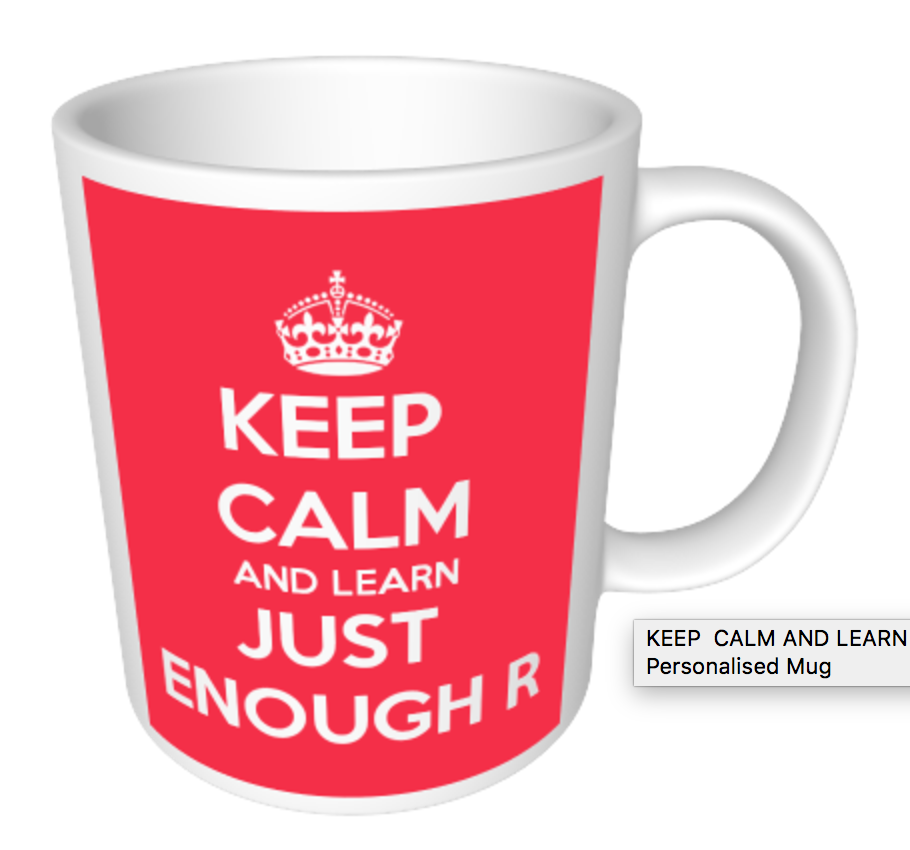
\includegraphics{media/keepcalm.png}

R makes it easy to work with and learn from data.

It also happens to be a programmming language, but if you're reading this, that
might not be of interest. That's OK --- the goal here is not to teach
programming\footnote{This is a lie, but hopefully it won't be obvious until it's too
  late.}. The goal is to teach you \emph{just enough R} to be confident to explore your
data.

This book uses R like any other statistics software: To work-with and visualise
data, run statistical analyses, and share our results with others. To do that
you don't need more than the \emph{absolute basics} of the R language itself. The
first chapters walk you through what you need to know to be productive.

\hypertarget{things-to-know-before-you-start}{%
\paragraph{Things to know Before you start}\label{things-to-know-before-you-start}}
\addcontentsline{toc}{paragraph}{Things to know Before you start}

This guide is fairly opinionated, but for good reason.

There are lots of ways to use R, and this has been a barrier for beginners. In
particular base-R functions can be oddly-named, or lack a regular or predictable
interface. For this reason we:

\begin{itemize}
\item
  Recommend (strongly) that you install and use `packages' that extend some of
  R's basic functionality. These packages are powerful tools in their own
  right, but also hide some of the complexities of R in a
  \href{https://www.youtube.com/watch?v=K-ss_ag2k9E}{clear and consistent way}. It
  might seem restrictive but, to begin with, learning \emph{only} these packages
  will help you form a more consistent mental model and make rapid progress.
  You can learn the crufty old bits (which still have their uses) later on.
\item
  Assume you are using the \protect\hyperlink{rstudio}{RStudio editor} and working in an
  \protect\hyperlink{rmarkdown}{RMarkdown document} (see the next section). If you don't have
  access to RStudio yet, see the \href{installation.html}{installation guide}.
\end{itemize}

\hypertarget{license}{%
\paragraph{License}\label{license}}
\addcontentsline{toc}{paragraph}{License}

These documents are licensed under the
\href{https://creativecommons.org/licenses/by-sa/4.0/}{CC BY-SA licence}.

\hypertarget{part-getting-started}{%
\part{Getting started}\label{part-getting-started}}

\hypertarget{r-basics}{%
\section{Working with R}\label{r-basics}}

There are many ways of working with R. This guide focusses on a fairly specific
setup and workflow, and assumes you will use the RStudio editor, use R markdown
documents to document and share your analyses, and install a number of recent
packages, including the `tidyverse', which give working with R a shallower
learning curve, and let you get powerful things done quickly.

\hypertarget{installation-intro}{%
\subsection*{Installation}\label{installation-intro}}
\addcontentsline{toc}{subsection}{Installation}

\hypertarget{local-install}{%
\paragraph{Installing on your own machine.}\label{local-install}}
\addcontentsline{toc}{paragraph}{Installing on your own machine.}

\begin{enumerate}
\def\labelenumi{\arabic{enumi}.}
\item
  \href{https://www.rstudio.com/products/rstudio/download/}{Download RStudio 1.01 or later}
  Use whatever version is most recent and expect to upgrade every 6 months or
  so, as new versions become available.
\item
  Install the \protect\hyperlink{dependencies}{packages listed below}
\item
  Optionally, if you want to `knit' your work into a pdf format, you should
  also install LaTeX. For most people this isn't necessary, and is something
  you can skip for the moment, but it can be helpful when sharing finished
  analyses with colleagues. On
  \href{https://miktex.org/download}{windows use this installer}. Make sure to do a
  `full install', not just a basic install. On a Mac install
  \href{https://brew.sh}{homebrew} and type \texttt{brew\ cask\ install\ mactex}.
\end{enumerate}

\hypertarget{dependencies}{%
\paragraph{Package dependencies}\label{dependencies}}
\addcontentsline{toc}{paragraph}{Package dependencies}

If you are just gettign started on a windows machine,
\href{https://github.com/PlymouthPsychology/installR/blob/master/install-windows-stage1.md}{these instructions for students at Plymouth University}
make it easy to install R and most of the packages necessary to complete the
examples in this book.

\href{https://github.com/PlymouthPsychology/installR}{Further details of a recommended installation are given here}.
These scripts will install all needed packages on a recent Linux or Mac system.

For some of the sections on Bayesian estimation you will also need to install
\texttt{rstan} and \texttt{rstanarm}.
\href{https://github.com/PlymouthPsychology/installR}{Details are also here}, but
this can wait till later.

\hypertarget{start-here}{%
\subsection*{Workflow}\label{start-here}}
\addcontentsline{toc}{subsection}{Workflow}

One big adjustment to make when moving away tools like SPSS is to find a `way of
working' that suits you.

We have often developed ways of working, saving, and communicating our work, and
become comfortable with them. In part, these habits and routines may be attempts
to work around limitations of these tools. But nevertheless, habits are easier
to replace than break, so here's an alternative model to adopt:

\begin{enumerate}
\def\labelenumi{\arabic{enumi}.}
\item
  Work in \protect\hyperlink{rstudio}{RStudio}, and use \protect\hyperlink{rmarkdown}{RMarkdown} documents (see
  next sections).
\item
  Save your raw data in \protect\hyperlink{use-csv}{.csv format}. Never edit data by hand unless
  absolutely necessary.
\item
  \protect\hyperlink{save-intermediate-steps}{Use R to process your data and RMarkdown to document the process}.
\end{enumerate}

\hypertarget{rmarkdown}{%
\subsubsection*{RMarkdown}\label{rmarkdown}}
\addcontentsline{toc}{subsubsection}{RMarkdown}

Conventional statistics software like SPSS lacks a simple way to document and
share your analyses, and make repeating or editing your work later very hard.

RMarkdown is a format for documenting and sharing statistical analyses.

This it might seem an odd place to start: we haven't got anything to share yet!
But using RMarkdown in RStudio provides a really nice way to work with data
interactively and share our results, so we start as we mean to go on.

You are currently reading the output of an `RMarkdown' document. An RMarkdown
document mixes R code with Markdown:

\begin{itemize}
\tightlist
\item
  R is a computer language designed for working with data.
\item
  Markdown is a simple text-based format which can include prose, hypertext
  links, images, and code (see \url{http://commonmark.org/help/}).
\end{itemize}

Like computer code, RMarkdown can be `run' or `executed'. But in the language of
RStudio, you `knit' your RMarkdown to produce a finished document. This combines
analyses, graphs, and explanatory text in a single pdf, html, or Word document
which can be shared.

\hypertarget{rstudio}{%
\subsubsection*{RStudio}\label{rstudio}}
\addcontentsline{toc}{subsubsection}{RStudio}

\href{https://www.rstudio.com/products/rstudio/}{RStudio} is a special text editor
that has been customised to make working with R easy. It can be installed on
your own computer, or you can login to a shared RStudio server (for example, one
run by your university) from a web browser. Either way the interface is largely
the same and contains 4 main panels:

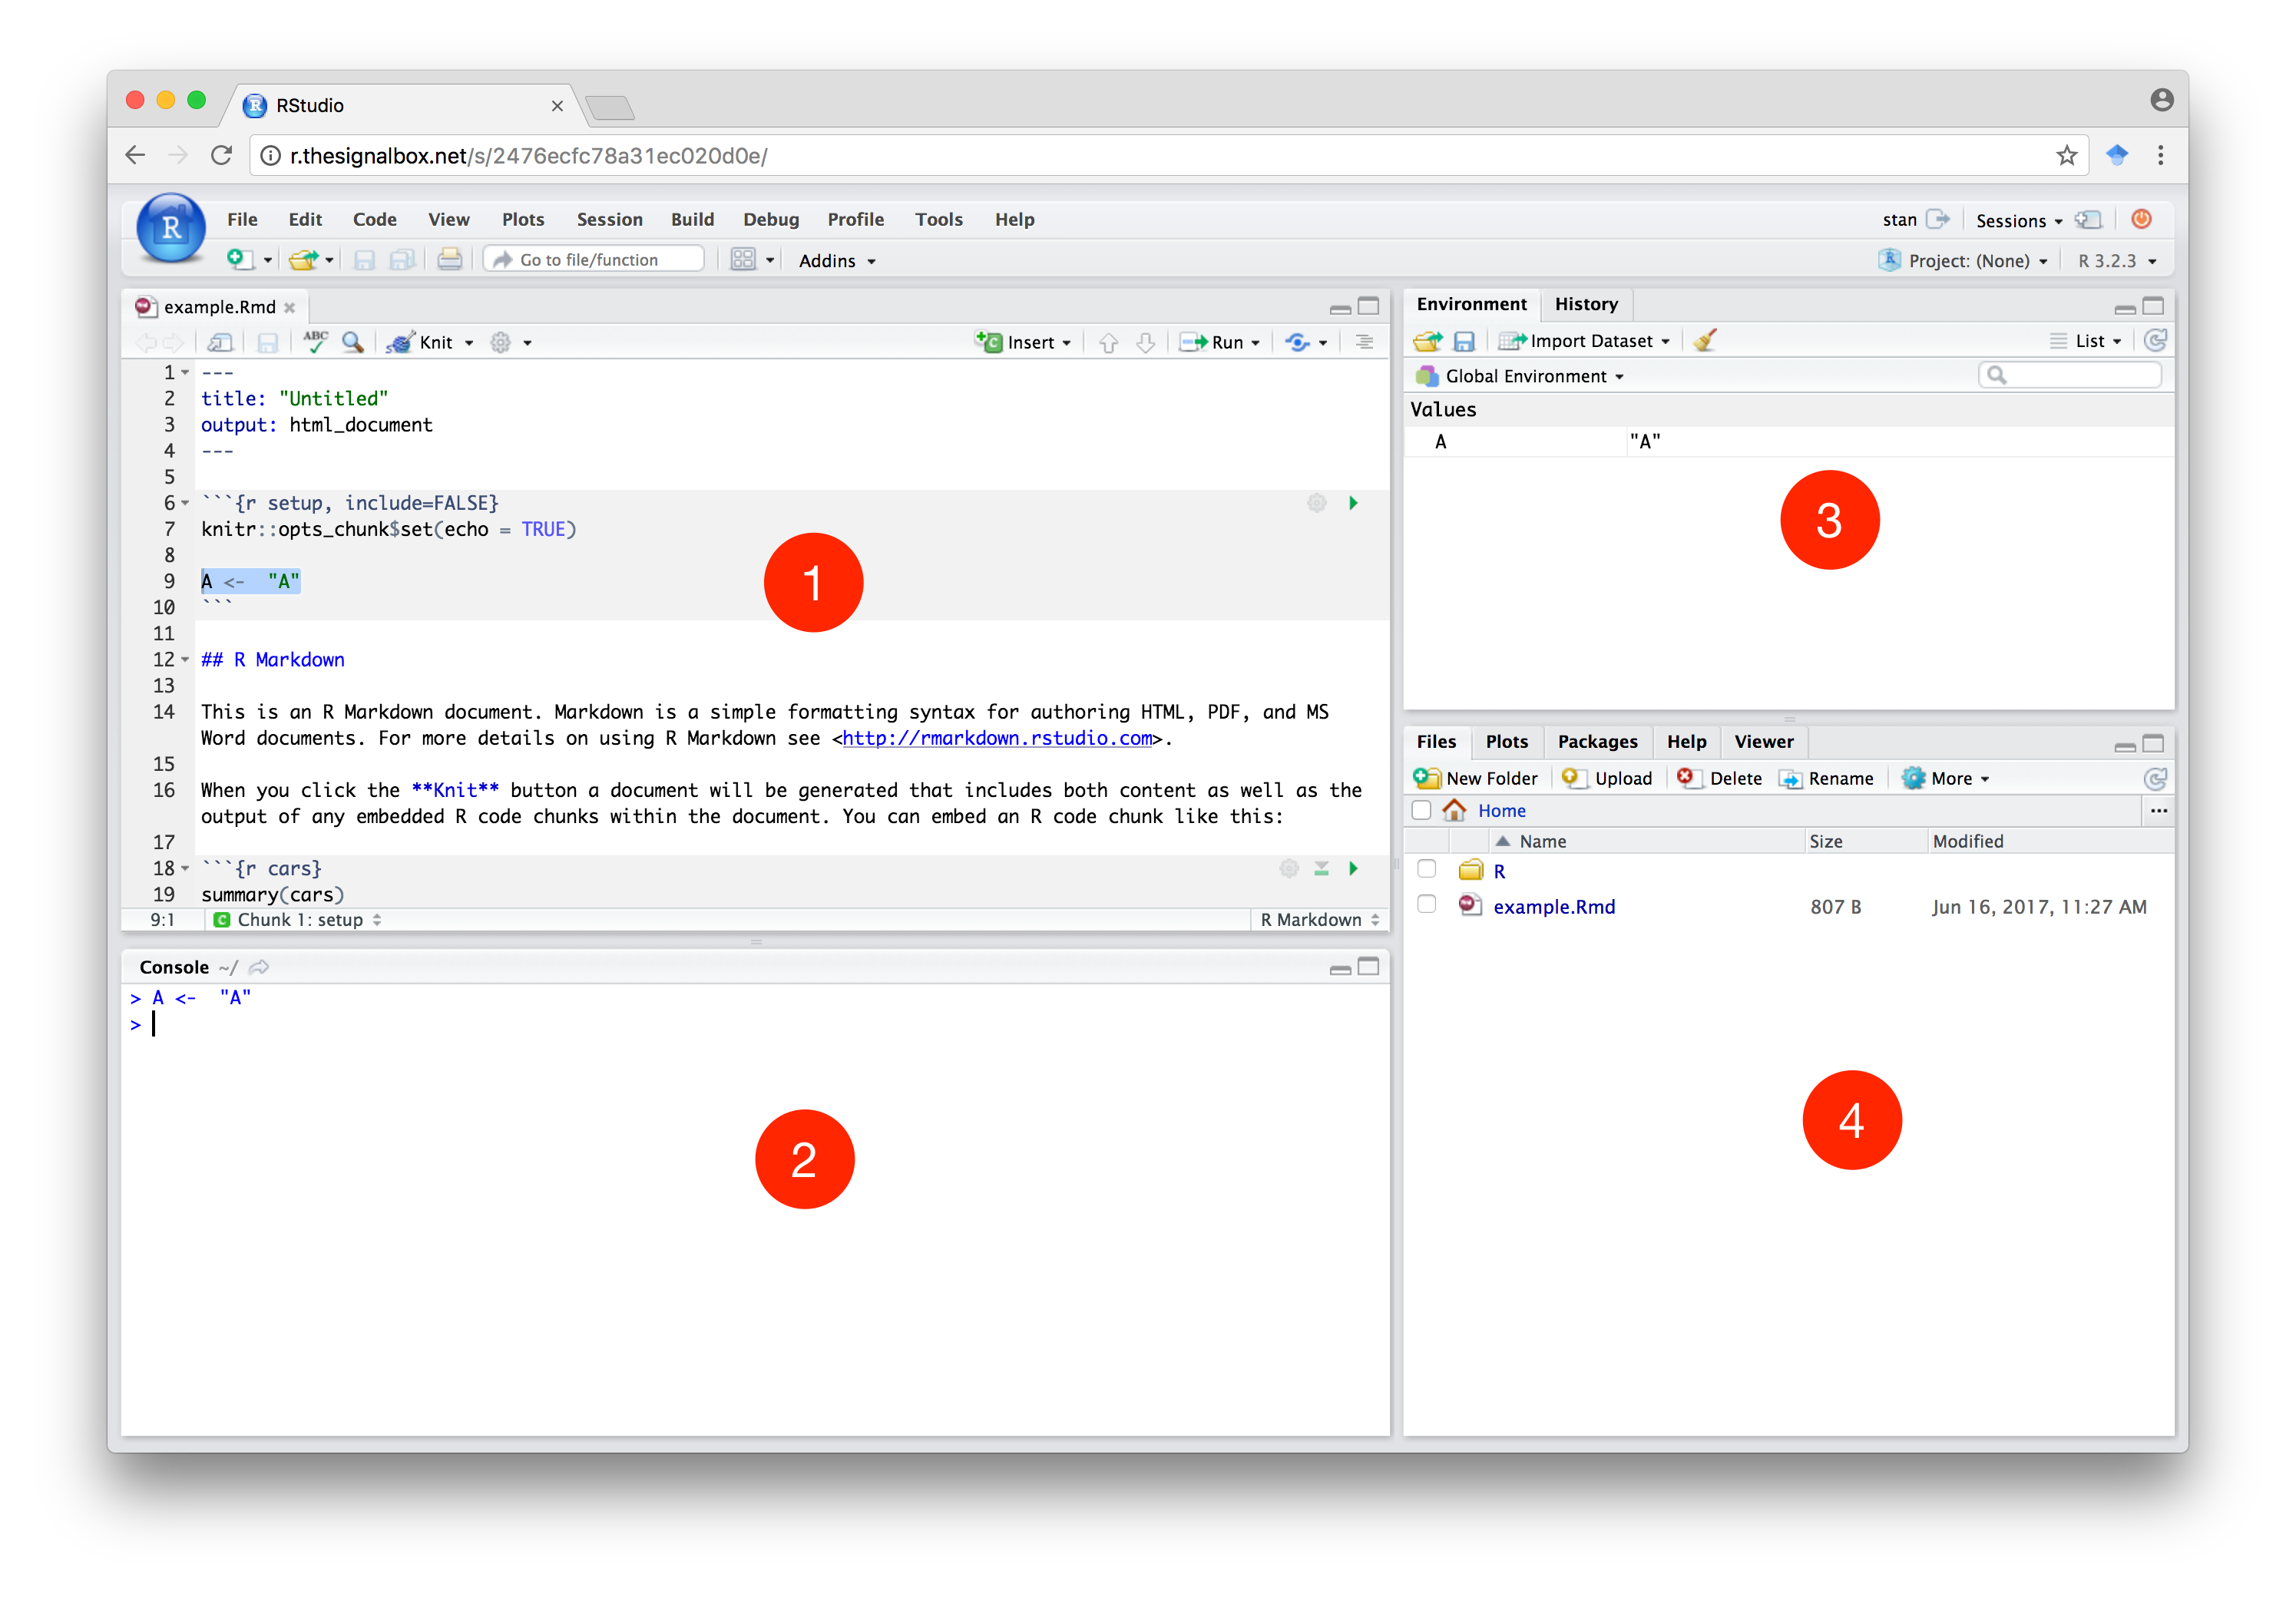
\includegraphics[width=41.53in]{media/rstudio-mainwindow}

The figure above shows the main RStudio interface, comprising:

\begin{enumerate}
\def\labelenumi{\arabic{enumi}.}
\item
  The main R-script or RMarkdown editor window. This is where you write
  commands, which can then be executed (to run the current line type ctrl-Enter
  or cmd-Enter on a Mac).
\item
  The R console, into which you can type R commands directly, and see the
  output of commands run in the script editor.
\item
  The `environment' panel, which lists all the variables you have defined and
  currently available to use.
\item
  The files and help panel. Within this panel the `files' tab enables you to
  open files stored on the server, in the current project, or elsewhere on your
  hard drive.
\end{enumerate}

You can see a short video demonstrating the RStudio interface here:

The video:

\begin{itemize}
\tightlist
\item
  Shows you how to type commands into the Console and view the results.
\item
  Run a plotting function, and see the result.
\item
  Create RMarkdown file, and `Knit' it to produce a document containing the
  results of your code and explanatory text.
\end{itemize}

Once you have watched the video:

\begin{itemize}
\tightlist
\item
  Open RStudio and create a new RMarkdown document.
\item
  Edit some of the text, and press the \texttt{Knit} button to see the results.
\item
  Edit some of the R blocks and see what happens.
\end{itemize}

\hypertarget{creating-code-chunks}{%
\subsubsection*{Creating code chunks}\label{creating-code-chunks}}
\addcontentsline{toc}{subsubsection}{Creating code chunks}

To include R code within RMarkdown we write 3 backticks (\texttt{\textasciigrave{}\textasciigrave{}\textasciigrave{}}), followed by
\texttt{\{r\}}. We the include our R code, and close the block with 3 more backticks
(\protect\hyperlink{backtick-location}{how to find the backtick on your keyboard}).

\begin{figure}
\centering
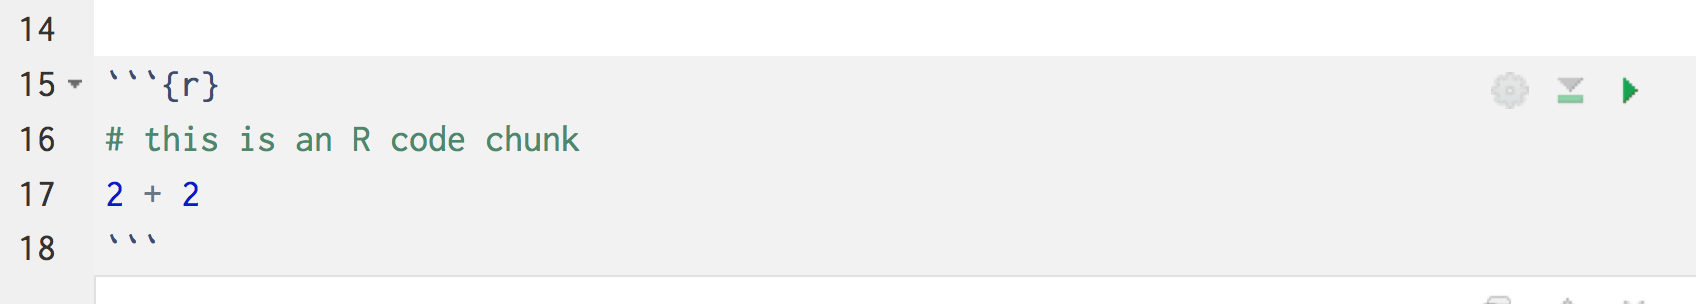
\includegraphics{media/r-code-chunk.png}
\caption{A code chunk in the RMarkdown editor}
\end{figure}

When a document including this chunk is run or `knitted', the final result will
include the the line \texttt{2+2} followed by the number \texttt{4} on the next line. We can
use RMarkdown to `show our workings': our analysis can be interleaved with
narrative text to explain or interpret the calculations.

\hypertarget{more-about-rmarkdown}{%
\subparagraph{More about RMarkdown}\label{more-about-rmarkdown}}
\addcontentsline{toc}{subparagraph}{More about RMarkdown}

A more in depth explanation of RMarkdown is here:
\url{https://rmarkdown.rstudio.com}, and a detailed
user guide here:
\url{https://rmarkdown.rstudio.com/lesson-1.html}

\hypertarget{first-commands}{%
\subsection*{First commands}\label{first-commands}}
\addcontentsline{toc}{subsection}{First commands}

You can type R commands directly into the `console' (see \protect\hyperlink{rstudio}{here}) and
see the result there, but you should make a habit of working in an RMarkdown
file. This keeps a record of everything you try, and makes it easy to edit/amend
things which didn't quite work.

Create a new Rmarkdown document from the `file' menu in RStudio.

\hypertarget{section}{%
\paragraph{}\label{section}}
\addcontentsline{toc}{paragraph}{}

To run code in the RStudio interface put your cursor on a line within an R Block
(or select the code you want to run), and press \texttt{Ctrl-Enter}. The result will
appear below the code block.

The command in the R block below prints (i.e.~shows on screen) the first few
rows of a dataset that is built-in to R as an example, called \texttt{mtcars}.

Place your cursor somewhere in the line the command is on and run it by typing
\texttt{Ctrl-Enter}, shown in this brief video:

Create an R block in RMarkdown, then run some simple commands.

\begin{Shaded}
\begin{Highlighting}[]
\KeywordTok{head}\NormalTok{(mtcars)}
\NormalTok{                   mpg cyl disp  hp drat    wt  qsec vs am gear carb}
\NormalTok{Mazda RX4         }\FloatTok{21.0}   \DecValTok{6}  \DecValTok{160} \DecValTok{110} \FloatTok{3.90} \FloatTok{2.620} \FloatTok{16.46}  \DecValTok{0}  \DecValTok{1}    \DecValTok{4}    \DecValTok{4}
\NormalTok{Mazda RX4 Wag     }\FloatTok{21.0}   \DecValTok{6}  \DecValTok{160} \DecValTok{110} \FloatTok{3.90} \FloatTok{2.875} \FloatTok{17.02}  \DecValTok{0}  \DecValTok{1}    \DecValTok{4}    \DecValTok{4}
\NormalTok{Datsun }\DecValTok{710}        \FloatTok{22.8}   \DecValTok{4}  \DecValTok{108}  \DecValTok{93} \FloatTok{3.85} \FloatTok{2.320} \FloatTok{18.61}  \DecValTok{1}  \DecValTok{1}    \DecValTok{4}    \DecValTok{1}
\NormalTok{Hornet }\DecValTok{4}\NormalTok{ Drive    }\FloatTok{21.4}   \DecValTok{6}  \DecValTok{258} \DecValTok{110} \FloatTok{3.08} \FloatTok{3.215} \FloatTok{19.44}  \DecValTok{1}  \DecValTok{0}    \DecValTok{3}    \DecValTok{1}
\NormalTok{Hornet Sportabout }\FloatTok{18.7}   \DecValTok{8}  \DecValTok{360} \DecValTok{175} \FloatTok{3.15} \FloatTok{3.440} \FloatTok{17.02}  \DecValTok{0}  \DecValTok{0}    \DecValTok{3}    \DecValTok{2}
\NormalTok{Valiant           }\FloatTok{18.1}   \DecValTok{6}  \DecValTok{225} \DecValTok{105} \FloatTok{2.76} \FloatTok{3.460} \FloatTok{20.22}  \DecValTok{1}  \DecValTok{0}    \DecValTok{3}    \DecValTok{1}
\end{Highlighting}
\end{Shaded}

If you are reading this from within RStudio, running \texttt{head(mtcars)} makes an
interactive table in your document, which you can use this to browse the
\texttt{mtcars} dataset.

If you are still reading the compiled html or pdf document you will see a static
table containing the same data.

Hopefully at this point it's obvious that RStudio and RMarkdown give you:

\begin{itemize}
\tightlist
\item
  A nice place to work your data interactively
\item
  A way to `show your workings' and save this for later
\item
  A way to share your analysis
\end{itemize}

\hypertarget{variables}{%
\subsection*{Naming things}\label{variables}}
\addcontentsline{toc}{subsection}{Naming things}

We can assign labels to the results of calculations and other parts of our
analyses to keep track of them.

To assign labels we use the \texttt{\textless{}-} symbol. The \texttt{\textless{}-} symbol points from the value
we want to store, to the name we want to use. For example:

\begin{Shaded}
\begin{Highlighting}[]
\NormalTok{the_magic_number <-}\StringTok{ }\DecValTok{3}
\end{Highlighting}
\end{Shaded}

This assigns the value \texttt{3} to the variable \texttt{the\_magic\_number}.

This block wouldn't display anything because assigning a variable doesn't create
any output.

To both assign a variable \emph{and} display it we would type:

\begin{Shaded}
\begin{Highlighting}[]
\NormalTok{the_magic_number <-}\StringTok{ }\DecValTok{3}
\NormalTok{the_magic_number}
\NormalTok{[}\DecValTok{1}\NormalTok{] }\DecValTok{3}
\end{Highlighting}
\end{Shaded}

Or we can use a shortcut: if we wrap the line in parentheses this both makes the
assignment and prints the result to the console:

\begin{Shaded}
\begin{Highlighting}[]
\NormalTok{(i_am_a_new_variable <-}\StringTok{ }\DecValTok{22}\NormalTok{)}
\NormalTok{[}\DecValTok{1}\NormalTok{] }\DecValTok{22}
\end{Highlighting}
\end{Shaded}

We can also do calculations as we assign variables:

\begin{Shaded}
\begin{Highlighting}[]
\NormalTok{one_score <-}\StringTok{ }\DecValTok{20}
\NormalTok{(four_score_years_and_ten <-}\StringTok{ }\NormalTok{one_score }\OperatorTok{*}\StringTok{ }\DecValTok{4} \OperatorTok{+}\StringTok{ }\DecValTok{10}\NormalTok{)}
\NormalTok{[}\DecValTok{1}\NormalTok{] }\DecValTok{90}
\end{Highlighting}
\end{Shaded}

We can give \emph{anything} a label by assigning it to a variable.

It doesn't have to be a number; we can also assign letters, words, graphics, the
results of a statistical model, or \emph{lists} of any of these things.

This will come in handy later.

\hypertarget{vectors-and-lists}{%
\subsection*{Vectors and lists}\label{vectors-and-lists}}
\addcontentsline{toc}{subsection}{Vectors and lists}

When working with data, we often have lists or sequences of `things'. For
example: a list of measurements we have made.

\begin{itemize}
\item
  When all the things are of the same type, R calls this a \emph{vector}\footnote{It's
    actually a matrix if has 2 dimensions, like a table, or an array if it has
    more than 2 dimensions.}.
\item
  When there is a mix of different things R calls this a \emph{list}.
\end{itemize}

\hypertarget{vector}{%
\subsubsection*{Vectors}\label{vector}}
\addcontentsline{toc}{subsubsection}{Vectors}

We can create a vector of numbers and display it like this:

\begin{Shaded}
\begin{Highlighting}[]
\CommentTok{# this creates a vector of heights, in cm}
\NormalTok{heights <-}\StringTok{ }\KeywordTok{c}\NormalTok{(}\DecValTok{203}\NormalTok{, }\DecValTok{148}\NormalTok{, }\DecValTok{156}\NormalTok{, }\DecValTok{158}\NormalTok{, }\DecValTok{167}\NormalTok{,}
             \DecValTok{162}\NormalTok{, }\DecValTok{172}\NormalTok{, }\DecValTok{164}\NormalTok{, }\DecValTok{172}\NormalTok{, }\DecValTok{187}\NormalTok{,}
             \DecValTok{134}\NormalTok{, }\DecValTok{182}\NormalTok{, }\DecValTok{175}\NormalTok{)}
\end{Highlighting}
\end{Shaded}

The \texttt{c()} command is shorthand for \emph{combine}, so the example above combines the
individual elements (numbers) into a new vector.

We can create a vector of alphanumeric names just as easily:

\begin{Shaded}
\begin{Highlighting}[]
\NormalTok{names <-}\StringTok{ }\KeywordTok{c}\NormalTok{(}\StringTok{"Ben"}\NormalTok{, }\StringTok{"Joe"}\NormalTok{, }\StringTok{"Sue"}\NormalTok{, }\StringTok{"Rosa"}\NormalTok{)}
\end{Highlighting}
\end{Shaded}

And we can check the values stored in these variables by printing them. You can
either type \texttt{print(heights)}, or just write the name of the variable alone,
which will print it by default. E.g.:

\begin{Shaded}
\begin{Highlighting}[]
\NormalTok{heights}
\NormalTok{ [}\DecValTok{1}\NormalTok{] }\DecValTok{203} \DecValTok{148} \DecValTok{156} \DecValTok{158} \DecValTok{167} \DecValTok{162} \DecValTok{172} \DecValTok{164} \DecValTok{172} \DecValTok{187} \DecValTok{134} \DecValTok{182} \DecValTok{175}
\end{Highlighting}
\end{Shaded}

\hypertarget{section-1}{%
\paragraph{}\label{section-1}}
\addcontentsline{toc}{paragraph}{}

Try creating your own vector of numbers in a new code block below\footnote{i.e.~edit the
  RMarkdown document} using the \texttt{c(...)} command. Then change the name of the
variable you assign it to.

\hypertarget{access-vector-elements}{%
\subsubsection*{Accessing elements}\label{access-vector-elements}}
\addcontentsline{toc}{subsubsection}{Accessing elements}

Once we have created a vector, we often want to access the individual elements
again. We do this based on their \emph{position}.

Let's say we have created a vector:

\begin{Shaded}
\begin{Highlighting}[]
\NormalTok{my.vector <-}\StringTok{ }\KeywordTok{c}\NormalTok{(}\DecValTok{10}\NormalTok{, }\DecValTok{20}\NormalTok{, }\DecValTok{30}\NormalTok{, }\DecValTok{40}\NormalTok{)}
\end{Highlighting}
\end{Shaded}

We can display the whole vector by just typing its name, as we saw above. But if
we want to show only the \emph{first} element of this vector, we type:

\begin{Shaded}
\begin{Highlighting}[]
\NormalTok{my.vector[}\DecValTok{1}\NormalTok{]}
\NormalTok{[}\DecValTok{1}\NormalTok{] }\DecValTok{10}
\end{Highlighting}
\end{Shaded}

Here, the square brackets specify a \emph{subset} of the vector we want - in this
case, just the first element.

\hypertarget{selecting-more-than-one-element}{%
\subsubsection*{Selecting more than one element}\label{selecting-more-than-one-element}}
\addcontentsline{toc}{subsubsection}{Selecting more than one element}

A neat feature of subsetting is that we can grab more than one element at a
time.

To do this, we need to tell R the \emph{positions} of the elements we want, and so we
provide a \emph{vector of the positions of the elements we want}.

It might seem obvious, but the first element has position 1, the second has
position 2, and so on. So, if we wanted to extract the 4th and 5th elements from
the vector of heights we saw above we would type:

\begin{Shaded}
\begin{Highlighting}[]
\NormalTok{elements.to.grab <-}\StringTok{ }\KeywordTok{c}\NormalTok{(}\DecValTok{4}\NormalTok{, }\DecValTok{5}\NormalTok{)}
\NormalTok{heights[elements.to.grab]}
\NormalTok{[}\DecValTok{1}\NormalTok{] }\DecValTok{158} \DecValTok{167}
\end{Highlighting}
\end{Shaded}

We can also make a subset of the original vector and assign it to a \emph{new}
variable:

\begin{Shaded}
\begin{Highlighting}[]
\NormalTok{first.two.elements <-}\StringTok{ }\NormalTok{heights[}\KeywordTok{c}\NormalTok{(}\DecValTok{1}\NormalTok{, }\DecValTok{2}\NormalTok{)]}
\NormalTok{first.two.elements}
\NormalTok{[}\DecValTok{1}\NormalTok{] }\DecValTok{203} \DecValTok{148}
\end{Highlighting}
\end{Shaded}

\hypertarget{making-sequences}{%
\subsubsection*{Making and slicing with sequences}\label{making-sequences}}
\addcontentsline{toc}{subsubsection}{Making and slicing with sequences}

One common task in R is to create sequences of numbers, letters or dates.

The simplest way of doing this is to define a range, with the colon:

\begin{Shaded}
\begin{Highlighting}[]
\NormalTok{onetoten <-}\StringTok{ }\DecValTok{1}\OperatorTok{:}\DecValTok{10}
\NormalTok{onetoten}
\NormalTok{ [}\DecValTok{1}\NormalTok{]  }\DecValTok{1}  \DecValTok{2}  \DecValTok{3}  \DecValTok{4}  \DecValTok{5}  \DecValTok{6}  \DecValTok{7}  \DecValTok{8}  \DecValTok{9} \DecValTok{10}
\end{Highlighting}
\end{Shaded}

This creates a vector which can be sliced like any other:

\begin{Shaded}
\begin{Highlighting}[]
\NormalTok{onetoten[}\DecValTok{8}\NormalTok{]}
\NormalTok{[}\DecValTok{1}\NormalTok{] }\DecValTok{8}
\end{Highlighting}
\end{Shaded}

One common use of sequences is to slice other vectors:

\begin{Shaded}
\begin{Highlighting}[]
\NormalTok{onetoten[}\DecValTok{1}\OperatorTok{:}\DecValTok{3}\NormalTok{]}
\NormalTok{[}\DecValTok{1}\NormalTok{] }\DecValTok{1} \DecValTok{2} \DecValTok{3}
\end{Highlighting}
\end{Shaded}

Or the first 10 values in the \texttt{heights} vector we defined above:

\begin{Shaded}
\begin{Highlighting}[]
\NormalTok{heights[}\DecValTok{1}\OperatorTok{:}\DecValTok{10}\NormalTok{]}
\NormalTok{ [}\DecValTok{1}\NormalTok{] }\DecValTok{203} \DecValTok{148} \DecValTok{156} \DecValTok{158} \DecValTok{167} \DecValTok{162} \DecValTok{172} \DecValTok{164} \DecValTok{172} \DecValTok{187}
\end{Highlighting}
\end{Shaded}

This works backwards, and with negative numbers too:

\begin{Shaded}
\begin{Highlighting}[]
\DecValTok{5}\OperatorTok{:-}\DecValTok{5}
\NormalTok{ [}\DecValTok{1}\NormalTok{]  }\DecValTok{5}  \DecValTok{4}  \DecValTok{3}  \DecValTok{2}  \DecValTok{1}  \DecValTok{0} \DecValTok{-1} \DecValTok{-2} \DecValTok{-3} \DecValTok{-4} \DecValTok{-5}
\end{Highlighting}
\end{Shaded}

When your sequence doesn't contain only whole numbers, or non-consecutive
numbers, you can use the \texttt{seq} function:

\begin{Shaded}
\begin{Highlighting}[]
\KeywordTok{seq}\NormalTok{(}\DecValTok{1}\NormalTok{,}\DecValTok{10}\NormalTok{,}\DataTypeTok{by=}\DecValTok{2}\NormalTok{)}
\NormalTok{[}\DecValTok{1}\NormalTok{] }\DecValTok{1} \DecValTok{3} \DecValTok{5} \DecValTok{7} \DecValTok{9}
\KeywordTok{seq}\NormalTok{(}\DecValTok{0}\NormalTok{, }\DecValTok{1}\NormalTok{, }\DataTypeTok{by=}\NormalTok{.}\DecValTok{2}\NormalTok{)}
\NormalTok{[}\DecValTok{1}\NormalTok{] }\FloatTok{0.0} \FloatTok{0.2} \FloatTok{0.4} \FloatTok{0.6} \FloatTok{0.8} \FloatTok{1.0}
\end{Highlighting}
\end{Shaded}

\hypertarget{conditional-slices}{%
\subsubsection*{Conditional slicing}\label{conditional-slices}}
\addcontentsline{toc}{subsubsection}{Conditional slicing}

One neat feature of R is that you can create a sequence of \texttt{TRUE} or \texttt{FALSE}
values, by asking whether each value in a sequence matches a particular
condition. For example:

\begin{Shaded}
\begin{Highlighting}[]
\DecValTok{1}\OperatorTok{:}\DecValTok{10} \OperatorTok{>}\StringTok{ }\DecValTok{5}
\NormalTok{ [}\DecValTok{1}\NormalTok{] }\OtherTok{FALSE} \OtherTok{FALSE} \OtherTok{FALSE} \OtherTok{FALSE} \OtherTok{FALSE}  \OtherTok{TRUE}  \OtherTok{TRUE}  \OtherTok{TRUE}  \OtherTok{TRUE}  \OtherTok{TRUE}
\end{Highlighting}
\end{Shaded}

Re-using the heights vector from above, we can then use this to select values
that are above the average:

\begin{Shaded}
\begin{Highlighting}[]
\NormalTok{heights }\OperatorTok{>}\StringTok{ }\KeywordTok{mean}\NormalTok{(heights)}
\NormalTok{ [}\DecValTok{1}\NormalTok{]  }\OtherTok{TRUE} \OtherTok{FALSE} \OtherTok{FALSE} \OtherTok{FALSE} \OtherTok{FALSE} \OtherTok{FALSE}  \OtherTok{TRUE} \OtherTok{FALSE}  \OtherTok{TRUE}  \OtherTok{TRUE} \OtherTok{FALSE}
\NormalTok{[}\DecValTok{12}\NormalTok{]  }\OtherTok{TRUE}  \OtherTok{TRUE}
\end{Highlighting}
\end{Shaded}

And we can use the vector of \texttt{TRUE} and \texttt{FALSE} values to select from the actual
scores:

\begin{Shaded}
\begin{Highlighting}[]
\NormalTok{heights[heights }\OperatorTok{>}\StringTok{ }\KeywordTok{mean}\NormalTok{(heights)]}
\NormalTok{[}\DecValTok{1}\NormalTok{] }\DecValTok{203} \DecValTok{172} \DecValTok{172} \DecValTok{187} \DecValTok{182} \DecValTok{175}
\end{Highlighting}
\end{Shaded}

\hypertarget{working-with-vectors}{%
\subsection*{Working with vectors}\label{working-with-vectors}}
\addcontentsline{toc}{subsection}{Working with vectors}

Many of R's most useful functions process \emph{vectors of numbers} in some way. For
example (as we've already seen) if we want to calculate the average of our
vector of heights we just type:

\begin{Shaded}
\begin{Highlighting}[]
\KeywordTok{mean}\NormalTok{(heights)}
\NormalTok{[}\DecValTok{1}\NormalTok{] }\FloatTok{167.6923}
\end{Highlighting}
\end{Shaded}

R contains \emph{lots} of built in functions which we can use to summarise a vector
of numbers. For example:

\begin{Shaded}
\begin{Highlighting}[]
\KeywordTok{median}\NormalTok{(heights)}
\NormalTok{[}\DecValTok{1}\NormalTok{] }\DecValTok{167}
\KeywordTok{sd}\NormalTok{(heights)}
\NormalTok{[}\DecValTok{1}\NormalTok{] }\FloatTok{17.59443}
\KeywordTok{min}\NormalTok{(heights)}
\NormalTok{[}\DecValTok{1}\NormalTok{] }\DecValTok{134}
\KeywordTok{max}\NormalTok{(heights)}
\NormalTok{[}\DecValTok{1}\NormalTok{] }\DecValTok{203}
\KeywordTok{range}\NormalTok{(heights)}
\NormalTok{[}\DecValTok{1}\NormalTok{] }\DecValTok{134} \DecValTok{203}
\KeywordTok{IQR}\NormalTok{(heights)}
\NormalTok{[}\DecValTok{1}\NormalTok{] }\DecValTok{17}
\KeywordTok{length}\NormalTok{(heights)}
\NormalTok{[}\DecValTok{1}\NormalTok{] }\DecValTok{13}
\end{Highlighting}
\end{Shaded}

All of these functions accept a vector as input, do some proccesing, and then
return a \emph{single number} which gets displayed by RStudio.

But not all functions return a single number in the way that \texttt{mean} did above.
Some return a new vector, or some other type of object instead. For example, the
\texttt{quantile} function returns the values at the 0, 25th, 50th, 75th and 100th
percentiles (by default).

\begin{Shaded}
\begin{Highlighting}[]
\NormalTok{height.quantiles <-}\StringTok{ }\KeywordTok{quantile}\NormalTok{(heights)}
\NormalTok{height.quantiles}
  \DecValTok{0}\OperatorTok\StringTok{  }\DecValTok{50}\OperatorTok\StringTok{ }\DecValTok{100}\NormalTok{% }
 \DecValTok{134}  \DecValTok{158}  \DecValTok{167}  \DecValTok{175}  \DecValTok{203} 
\end{Highlighting}
\end{Shaded}

If a function returns a vector, we can use it just like any other vector:

\begin{Shaded}
\begin{Highlighting}[]
\NormalTok{height.quantiles <-}\StringTok{ }\KeywordTok{quantile}\NormalTok{(heights)}

\CommentTok{# grab the third element, which is the median}
\NormalTok{height.quantiles[}\DecValTok{3}\NormalTok{]}
\DecValTok{50}\NormalTok{% }
\DecValTok{167} 

\CommentTok{# assign the first element to a variable}
\NormalTok{min.height <-}\StringTok{ }\NormalTok{height.quantiles[}\DecValTok{1}\NormalTok{]}
\NormalTok{min.height}
 \DecValTok{0}\NormalTok{% }
\DecValTok{134} 
\end{Highlighting}
\end{Shaded}

But other functions process a vector without returning any numbers. For example,
the \texttt{hist} function returns a histogram:

\begin{Shaded}
\begin{Highlighting}[]
\KeywordTok{hist}\NormalTok{(heights)}
\end{Highlighting}
\end{Shaded}

\includegraphics{start_here_files/figure-latex/unnamed-chunk-28-1.pdf}

We'll cover lots more plotting and visualisation later on.

\hypertarget{making-new-vectors}{%
\subsubsection*{Making new vectors}\label{making-new-vectors}}
\addcontentsline{toc}{subsubsection}{Making new vectors}

So far we've seen R functions which process a vector of numbers and produce a
single number, a new vector of a different length (like \texttt{quantile} or
\texttt{fivenum}), or some other object (like \texttt{hist} which makes a plot). However many
other functions accept a single input, do something to it, and return a single
processed value.

For example, the square root function, \texttt{sqrt}, accepts a single value and
returns a single value: running \texttt{sqrt(10)} will return \texttt{3.1623}.

In R, if a function accepts a single value as input and returns a single value
as output (like \texttt{sqrt(10)}), then you can usually give a vector as input too.
Some people find this surprising\footnote{Mostly people who already know other
  programming languages like C. It's not that surprising if you read the R code as
  you would English.}, but R assumes that if you're processing a vector of
numbers, you want the function applied to each of them in the same way.

This turns out to be very useful. For example, let's say we want the square root
of each of the elements of our height data:

\begin{Shaded}
\begin{Highlighting}[]
\CommentTok{# these are the raw values}
\NormalTok{heights}
\NormalTok{ [}\DecValTok{1}\NormalTok{] }\DecValTok{203} \DecValTok{148} \DecValTok{156} \DecValTok{158} \DecValTok{167} \DecValTok{162} \DecValTok{172} \DecValTok{164} \DecValTok{172} \DecValTok{187} \DecValTok{134} \DecValTok{182} \DecValTok{175}

\CommentTok{# takes the sqrt of each value and returns a vector of all the square roots}
\KeywordTok{sqrt}\NormalTok{(heights)}
\NormalTok{ [}\DecValTok{1}\NormalTok{] }\FloatTok{14.24781} \FloatTok{12.16553} \FloatTok{12.49000} \FloatTok{12.56981} \FloatTok{12.92285} \FloatTok{12.72792} \FloatTok{13.11488}
\NormalTok{ [}\DecValTok{8}\NormalTok{] }\FloatTok{12.80625} \FloatTok{13.11488} \FloatTok{13.67479} \FloatTok{11.57584} \FloatTok{13.49074} \FloatTok{13.22876}
\end{Highlighting}
\end{Shaded}

This also works with simple arithmetic So, if we wanted to convert all the
heights from cm to meters we could just type:

\begin{Shaded}
\begin{Highlighting}[]
\NormalTok{heights }\OperatorTok{/}\StringTok{ }\DecValTok{100}
\NormalTok{ [}\DecValTok{1}\NormalTok{] }\FloatTok{2.03} \FloatTok{1.48} \FloatTok{1.56} \FloatTok{1.58} \FloatTok{1.67} \FloatTok{1.62} \FloatTok{1.72} \FloatTok{1.64} \FloatTok{1.72} \FloatTok{1.87} \FloatTok{1.34} \FloatTok{1.82} \FloatTok{1.75}
\end{Highlighting}
\end{Shaded}

This trick also works with other functions like \texttt{paste}, which combines the
inputs you send it to produce an alphanumeric string:

\begin{Shaded}
\begin{Highlighting}[]
\KeywordTok{paste}\NormalTok{(}\StringTok{"Once"}\NormalTok{, }\StringTok{"upon"}\NormalTok{, }\StringTok{"a"}\NormalTok{, }\StringTok{"time"}\NormalTok{)}
\NormalTok{[}\DecValTok{1}\NormalTok{] }\StringTok{"Once upon a time"}
\end{Highlighting}
\end{Shaded}

If we send a vector to \texttt{paste} it assumes we want a vector of results, with each
element in the vector pasted next to each other:

\begin{Shaded}
\begin{Highlighting}[]
\NormalTok{bottles <-}\StringTok{ }\KeywordTok{c}\NormalTok{(}\DecValTok{100}\NormalTok{, }\DecValTok{99}\NormalTok{, }\DecValTok{98}\NormalTok{, }\StringTok{"..."}\NormalTok{)}
\KeywordTok{paste}\NormalTok{(bottles, }\StringTok{"green bottles hanging on the wall"}\NormalTok{)}
\NormalTok{[}\DecValTok{1}\NormalTok{] }\StringTok{"100 green bottles hanging on the wall"}
\NormalTok{[}\DecValTok{2}\NormalTok{] }\StringTok{"99 green bottles hanging on the wall"} 
\NormalTok{[}\DecValTok{3}\NormalTok{] }\StringTok{"98 green bottles hanging on the wall"} 
\NormalTok{[}\DecValTok{4}\NormalTok{] }\StringTok{"... green bottles hanging on the wall"}
\end{Highlighting}
\end{Shaded}

In other programming languages we might have had to write a `loop' to create
each line of the song, but R lets us write short statements to summarise \emph{what}
needs to be done; we don't need to worry worrying about \emph{how} it gets done.

\hypertarget{paste0}{%
\paragraph{}\label{paste0}}
\addcontentsline{toc}{paragraph}{}

The \texttt{paste0} function does much the same, but leaves no spaces in the combined
strings, which can be useful:

\begin{Shaded}
\begin{Highlighting}[]
\KeywordTok{paste0}\NormalTok{(}\StringTok{"N="}\NormalTok{, }\DecValTok{1}\OperatorTok{:}\DecValTok{10}\NormalTok{)}
\NormalTok{ [}\DecValTok{1}\NormalTok{] }\StringTok{"N=1"}  \StringTok{"N=2"}  \StringTok{"N=3"}  \StringTok{"N=4"}  \StringTok{"N=5"}  \StringTok{"N=6"}  \StringTok{"N=7"}  \StringTok{"N=8"}  \StringTok{"N=9"}  \StringTok{"N=10"}
\end{Highlighting}
\end{Shaded}

\hypertarget{making-up-data-new-vectors}{%
\subsubsection*{Making up data (new vectors)}\label{making-up-data-new-vectors}}
\addcontentsline{toc}{subsubsection}{Making up data (new vectors)}

Sometimes you'll need to create vectors containing regular sequences or randomly
selected numbers.

To create regular sequences a convenient shortcut is the `colon' operator. For
example, if we type \texttt{1:10} then we get a vector of numbers from 1 to 10:

\begin{Shaded}
\begin{Highlighting}[]
\DecValTok{1}\OperatorTok{:}\DecValTok{10}
\NormalTok{ [}\DecValTok{1}\NormalTok{]  }\DecValTok{1}  \DecValTok{2}  \DecValTok{3}  \DecValTok{4}  \DecValTok{5}  \DecValTok{6}  \DecValTok{7}  \DecValTok{8}  \DecValTok{9} \DecValTok{10}
\end{Highlighting}
\end{Shaded}

The \texttt{seq} function allows you to create more specific sequences:

\begin{Shaded}
\begin{Highlighting}[]
\CommentTok{# make a sequence, specifying the interval between them}
\KeywordTok{seq}\NormalTok{(}\DataTypeTok{from=}\FloatTok{0.1}\NormalTok{, }\DataTypeTok{to=}\DecValTok{2}\NormalTok{, }\DataTypeTok{by=}\NormalTok{.}\DecValTok{1}\NormalTok{)}
\NormalTok{ [}\DecValTok{1}\NormalTok{] }\FloatTok{0.1} \FloatTok{0.2} \FloatTok{0.3} \FloatTok{0.4} \FloatTok{0.5} \FloatTok{0.6} \FloatTok{0.7} \FloatTok{0.8} \FloatTok{0.9} \FloatTok{1.0} \FloatTok{1.1} \FloatTok{1.2} \FloatTok{1.3} \FloatTok{1.4} \FloatTok{1.5} \FloatTok{1.6} \FloatTok{1.7}
\NormalTok{[}\DecValTok{18}\NormalTok{] }\FloatTok{1.8} \FloatTok{1.9} \FloatTok{2.0}
\end{Highlighting}
\end{Shaded}

We can also use random number-generating functions built into R to create
vectors:

\begin{Shaded}
\begin{Highlighting}[]
\CommentTok{# 10 uniformly distributed random numbers between 0 and 1}
\KeywordTok{runif}\NormalTok{(}\DecValTok{10}\NormalTok{)}
\NormalTok{ [}\DecValTok{1}\NormalTok{] }\FloatTok{0.68178208} \FloatTok{0.90411456} \FloatTok{0.50615136} \FloatTok{0.98745549} \FloatTok{0.45402399} \FloatTok{0.03190653}
\NormalTok{ [}\DecValTok{7}\NormalTok{] }\FloatTok{0.91578234} \FloatTok{0.99891484} \FloatTok{0.61407334} \FloatTok{0.11438643}

\CommentTok{# 1,000 uniformly distributed random numbers between 1 and 100}
\NormalTok{my.numbers <-}\StringTok{ }\KeywordTok{runif}\NormalTok{(}\DecValTok{1000}\NormalTok{, }\DecValTok{1}\NormalTok{, }\DecValTok{10}\NormalTok{)}

\CommentTok{# 10 random-normal numbers with mean 10 and SD=1}
\KeywordTok{rnorm}\NormalTok{(}\DecValTok{10}\NormalTok{, }\DataTypeTok{mean=}\DecValTok{10}\NormalTok{)}
\NormalTok{ [}\DecValTok{1}\NormalTok{] }\FloatTok{10.748900} \FloatTok{10.159444}  \FloatTok{9.888892} \FloatTok{11.338383}  \FloatTok{7.736228}  \FloatTok{9.424838} \FloatTok{11.330858}
\NormalTok{ [}\DecValTok{8}\NormalTok{]  }\FloatTok{8.327885}  \FloatTok{9.348344}  \FloatTok{8.853372}

\CommentTok{# 10 random-normal numbers with mean 10 and SD=5}
\KeywordTok{rnorm}\NormalTok{(}\DecValTok{10}\NormalTok{, }\DecValTok{10}\NormalTok{, }\DecValTok{5}\NormalTok{)}
\NormalTok{ [}\DecValTok{1}\NormalTok{] }\FloatTok{11.7342244}  \FloatTok{7.9680336}  \FloatTok{7.9065691}  \FloatTok{9.5719237}  \FloatTok{8.1691346} \FloatTok{10.3218285}
\NormalTok{ [}\DecValTok{7}\NormalTok{] }\FloatTok{12.1666092}  \FloatTok{5.5941250} \FloatTok{17.7576063} \FloatTok{-0.7157989}
\end{Highlighting}
\end{Shaded}

We can then use these numbers in our code, for example plotting them:

\begin{Shaded}
\begin{Highlighting}[]
\NormalTok{random.numbers <-}\StringTok{ }\KeywordTok{rnorm}\NormalTok{(}\DecValTok{10000}\NormalTok{)}
\KeywordTok{hist}\NormalTok{(random.numbers)}
\end{Highlighting}
\end{Shaded}

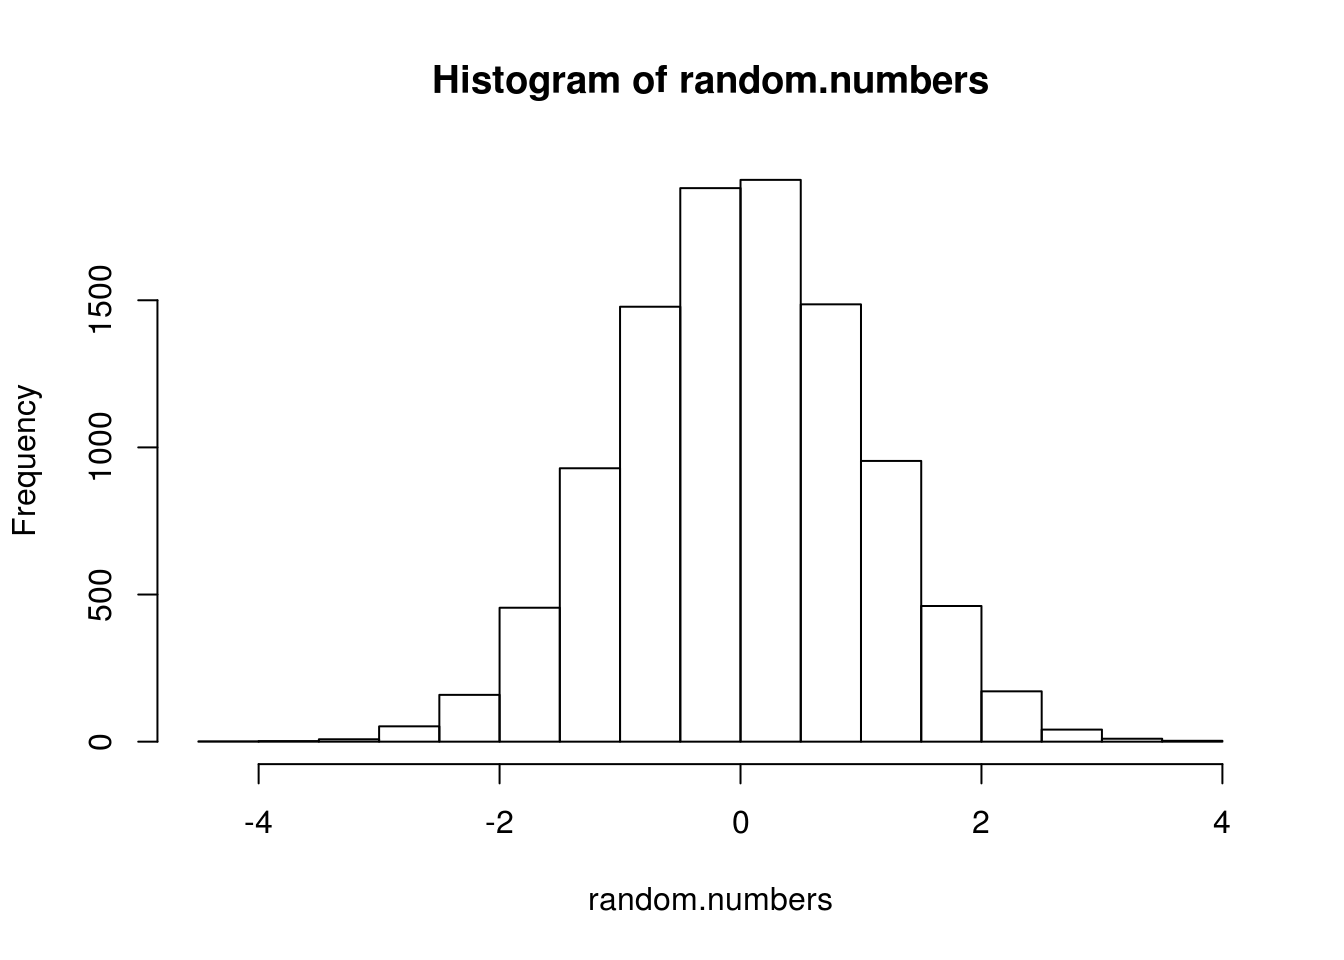
\includegraphics{start_here_files/figure-latex/unnamed-chunk-37-1.pdf}

\hypertarget{functions-to-learn-now}{%
\subsection*{Functions to learn now}\label{functions-to-learn-now}}
\addcontentsline{toc}{subsection}{Functions to learn now}

There are \emph{thousands} of functions built into R. Below are just a few examples
which are likely to be useful as you work with your data:

Repetition

\begin{Shaded}
\begin{Highlighting}[]
\CommentTok{# repeat something N times}
\KeywordTok{rep}\NormalTok{(}\StringTok{"Apple pie"}\NormalTok{, }\DecValTok{10}\NormalTok{)}
\NormalTok{ [}\DecValTok{1}\NormalTok{] }\StringTok{"Apple pie"} \StringTok{"Apple pie"} \StringTok{"Apple pie"} \StringTok{"Apple pie"} \StringTok{"Apple pie"}
\NormalTok{ [}\DecValTok{6}\NormalTok{] }\StringTok{"Apple pie"} \StringTok{"Apple pie"} \StringTok{"Apple pie"} \StringTok{"Apple pie"} \StringTok{"Apple pie"}
\end{Highlighting}
\end{Shaded}

\begin{Shaded}
\begin{Highlighting}[]
\CommentTok{# repeat a short vector, combining into a single longer vector}
\KeywordTok{rep}\NormalTok{(}\KeywordTok{c}\NormalTok{(}\StringTok{"Custard"}\NormalTok{, }\StringTok{"Gravy"}\NormalTok{), }\DecValTok{5}\NormalTok{)}
\NormalTok{ [}\DecValTok{1}\NormalTok{] }\StringTok{"Custard"} \StringTok{"Gravy"}   \StringTok{"Custard"} \StringTok{"Gravy"}   \StringTok{"Custard"} \StringTok{"Gravy"}   \StringTok{"Custard"}
\NormalTok{ [}\DecValTok{8}\NormalTok{] }\StringTok{"Gravy"}   \StringTok{"Custard"} \StringTok{"Gravy"}  
\end{Highlighting}
\end{Shaded}

Sequences

\begin{Shaded}
\begin{Highlighting}[]
\CommentTok{# make a sequence}
\NormalTok{(countdown <-}\StringTok{ }\DecValTok{100}\OperatorTok{:}\DecValTok{1}\NormalTok{)}
\NormalTok{  [}\DecValTok{1}\NormalTok{] }\DecValTok{100}  \DecValTok{99}  \DecValTok{98}  \DecValTok{97}  \DecValTok{96}  \DecValTok{95}  \DecValTok{94}  \DecValTok{93}  \DecValTok{92}  \DecValTok{91}  \DecValTok{90}  \DecValTok{89}  \DecValTok{88}  \DecValTok{87}  \DecValTok{86}  \DecValTok{85}  \DecValTok{84}
\NormalTok{ [}\DecValTok{18}\NormalTok{]  }\DecValTok{83}  \DecValTok{82}  \DecValTok{81}  \DecValTok{80}  \DecValTok{79}  \DecValTok{78}  \DecValTok{77}  \DecValTok{76}  \DecValTok{75}  \DecValTok{74}  \DecValTok{73}  \DecValTok{72}  \DecValTok{71}  \DecValTok{70}  \DecValTok{69}  \DecValTok{68}  \DecValTok{67}
\NormalTok{ [}\DecValTok{35}\NormalTok{]  }\DecValTok{66}  \DecValTok{65}  \DecValTok{64}  \DecValTok{63}  \DecValTok{62}  \DecValTok{61}  \DecValTok{60}  \DecValTok{59}  \DecValTok{58}  \DecValTok{57}  \DecValTok{56}  \DecValTok{55}  \DecValTok{54}  \DecValTok{53}  \DecValTok{52}  \DecValTok{51}  \DecValTok{50}
\NormalTok{ [}\DecValTok{52}\NormalTok{]  }\DecValTok{49}  \DecValTok{48}  \DecValTok{47}  \DecValTok{46}  \DecValTok{45}  \DecValTok{44}  \DecValTok{43}  \DecValTok{42}  \DecValTok{41}  \DecValTok{40}  \DecValTok{39}  \DecValTok{38}  \DecValTok{37}  \DecValTok{36}  \DecValTok{35}  \DecValTok{34}  \DecValTok{33}
\NormalTok{ [}\DecValTok{69}\NormalTok{]  }\DecValTok{32}  \DecValTok{31}  \DecValTok{30}  \DecValTok{29}  \DecValTok{28}  \DecValTok{27}  \DecValTok{26}  \DecValTok{25}  \DecValTok{24}  \DecValTok{23}  \DecValTok{22}  \DecValTok{21}  \DecValTok{20}  \DecValTok{19}  \DecValTok{18}  \DecValTok{17}  \DecValTok{16}
\NormalTok{ [}\DecValTok{86}\NormalTok{]  }\DecValTok{15}  \DecValTok{14}  \DecValTok{13}  \DecValTok{12}  \DecValTok{11}  \DecValTok{10}   \DecValTok{9}   \DecValTok{8}   \DecValTok{7}   \DecValTok{6}   \DecValTok{5}   \DecValTok{4}   \DecValTok{3}   \DecValTok{2}   \DecValTok{1}
\end{Highlighting}
\end{Shaded}

Make sequences with steps of a particular size:

\begin{Shaded}
\begin{Highlighting}[]
\NormalTok{(tenths  <-}\StringTok{ }\KeywordTok{seq}\NormalTok{(}\DataTypeTok{from=}\DecValTok{0}\NormalTok{, }\DataTypeTok{to=}\DecValTok{1}\NormalTok{, }\DataTypeTok{by=}\NormalTok{.}\DecValTok{1}\NormalTok{))}
\NormalTok{ [}\DecValTok{1}\NormalTok{] }\FloatTok{0.0} \FloatTok{0.1} \FloatTok{0.2} \FloatTok{0.3} \FloatTok{0.4} \FloatTok{0.5} \FloatTok{0.6} \FloatTok{0.7} \FloatTok{0.8} \FloatTok{0.9} \FloatTok{1.0}

\NormalTok{(twelfths <-}\StringTok{ }\KeywordTok{seq}\NormalTok{(}\DataTypeTok{from=}\DecValTok{0}\NormalTok{, }\DataTypeTok{to=}\DecValTok{10}\NormalTok{, }\DataTypeTok{length.out=}\DecValTok{12}\NormalTok{))}
\NormalTok{ [}\DecValTok{1}\NormalTok{]  }\FloatTok{0.0000000}  \FloatTok{0.9090909}  \FloatTok{1.8181818}  \FloatTok{2.7272727}  \FloatTok{3.6363636}  \FloatTok{4.5454545}
\NormalTok{ [}\DecValTok{7}\NormalTok{]  }\FloatTok{5.4545455}  \FloatTok{6.3636364}  \FloatTok{7.2727273}  \FloatTok{8.1818182}  \FloatTok{9.0909091} \FloatTok{10.0000000}
\end{Highlighting}
\end{Shaded}

Ranking

\begin{Shaded}
\begin{Highlighting}[]
\CommentTok{# generate some random data (here, ages in years)}
\NormalTok{ages <-}\StringTok{ }\KeywordTok{round}\NormalTok{(}\KeywordTok{rnorm}\NormalTok{(}\DecValTok{10}\NormalTok{, }\DataTypeTok{mean=}\DecValTok{40}\NormalTok{, }\DataTypeTok{sd=}\DecValTok{10}\NormalTok{))}

\CommentTok{# get the rank order of elements (i.e. what their positions would be if the vector was sorted)}
\NormalTok{ages}
\NormalTok{ [}\DecValTok{1}\NormalTok{] }\DecValTok{54} \DecValTok{48} \DecValTok{40} \DecValTok{53} \DecValTok{39} \DecValTok{27} \DecValTok{41} \DecValTok{21} \DecValTok{35} \DecValTok{42}
\KeywordTok{rank}\NormalTok{(ages, }\DataTypeTok{ties.method=}\StringTok{"first"}\NormalTok{)}
\NormalTok{ [}\DecValTok{1}\NormalTok{] }\DecValTok{10}  \DecValTok{8}  \DecValTok{5}  \DecValTok{9}  \DecValTok{4}  \DecValTok{2}  \DecValTok{6}  \DecValTok{1}  \DecValTok{3}  \DecValTok{7}
\end{Highlighting}
\end{Shaded}

Unique values

\begin{Shaded}
\begin{Highlighting}[]
\CommentTok{# return the unique values in a vector}
\KeywordTok{unique}\NormalTok{(}\KeywordTok{rep}\NormalTok{(}\DecValTok{1}\OperatorTok{:}\DecValTok{10}\NormalTok{, }\DecValTok{100}\NormalTok{))}
\NormalTok{ [}\DecValTok{1}\NormalTok{]  }\DecValTok{1}  \DecValTok{2}  \DecValTok{3}  \DecValTok{4}  \DecValTok{5}  \DecValTok{6}  \DecValTok{7}  \DecValTok{8}  \DecValTok{9} \DecValTok{10}
\end{Highlighting}
\end{Shaded}

Lengths

\begin{Shaded}
\begin{Highlighting}[]
\CommentTok{# return the unique values in a vector}
\KeywordTok{length}\NormalTok{(}\KeywordTok{seq}\NormalTok{(}\DecValTok{1}\NormalTok{,}\DecValTok{100}\NormalTok{, }\DecValTok{2}\NormalTok{))}
\NormalTok{[}\DecValTok{1}\NormalTok{] }\DecValTok{50}
\end{Highlighting}
\end{Shaded}

Try and experiment with each of these functions. Check the output against what
you expected to happen, and make sure you understand what they do.

\hypertarget{packages}{%
\subsection*{Packages}\label{packages}}
\addcontentsline{toc}{subsection}{Packages}

R has been around for ages. It remains popular because it's \emph{easy for people to
add to it}.

You can run almost any statistical model and produce many different plots in R
because users write `packages' which extend the base language. For now we assume
someone has helped you install all the packages you need\footnote{See the
  \href{installation.html}{installation guide} if this isn't the case}.

To \emph{access} features in packages, you normally load the package with the
\texttt{library()} function. Running \texttt{library(\textless{}packagename\textgreater{})} loads all the new
functions within it, and it is then possible to call them from your code. For
example, typing:

\begin{Shaded}
\begin{Highlighting}[]
\KeywordTok{library}\NormalTok{(ggplot2)}
\end{Highlighting}
\end{Shaded}

Will load the \texttt{ggplot2} package. You can then call the \texttt{qplot} function it
provides:

\begin{Shaded}
\begin{Highlighting}[]
\KeywordTok{qplot}\NormalTok{(mtcars}\OperatorTok{$}\NormalTok{mpg, }\DataTypeTok{bins=}\DecValTok{7}\NormalTok{)}
\end{Highlighting}
\end{Shaded}

\includegraphics{packages_files/figure-latex/unnamed-chunk-4-1.pdf}

It's good style to load packages at the top of an R script, or in the first
chunk of an RMarkdown document. This makes it easy for others to see what
packages they need to install, and helps avoid certain sorts of errors in your
code.

\hypertarget{package-namespacing}{%
\paragraph{}\label{package-namespacing}}
\addcontentsline{toc}{paragraph}{}

You don't strictly \emph{need} to load packages to use their features. If a package
is installed on your system you can also call a function it provides directly.
In the example below we call the \texttt{hist.data.frame} from the \texttt{Hmisc} package, and
obtain histograms of all the variables in the \texttt{mtcars} dataset:

\begin{Shaded}
\begin{Highlighting}[]
\NormalTok{Hmisc}\OperatorTok{::}\KeywordTok{hist.data.frame}\NormalTok{(mtcars)}
\end{Highlighting}
\end{Shaded}

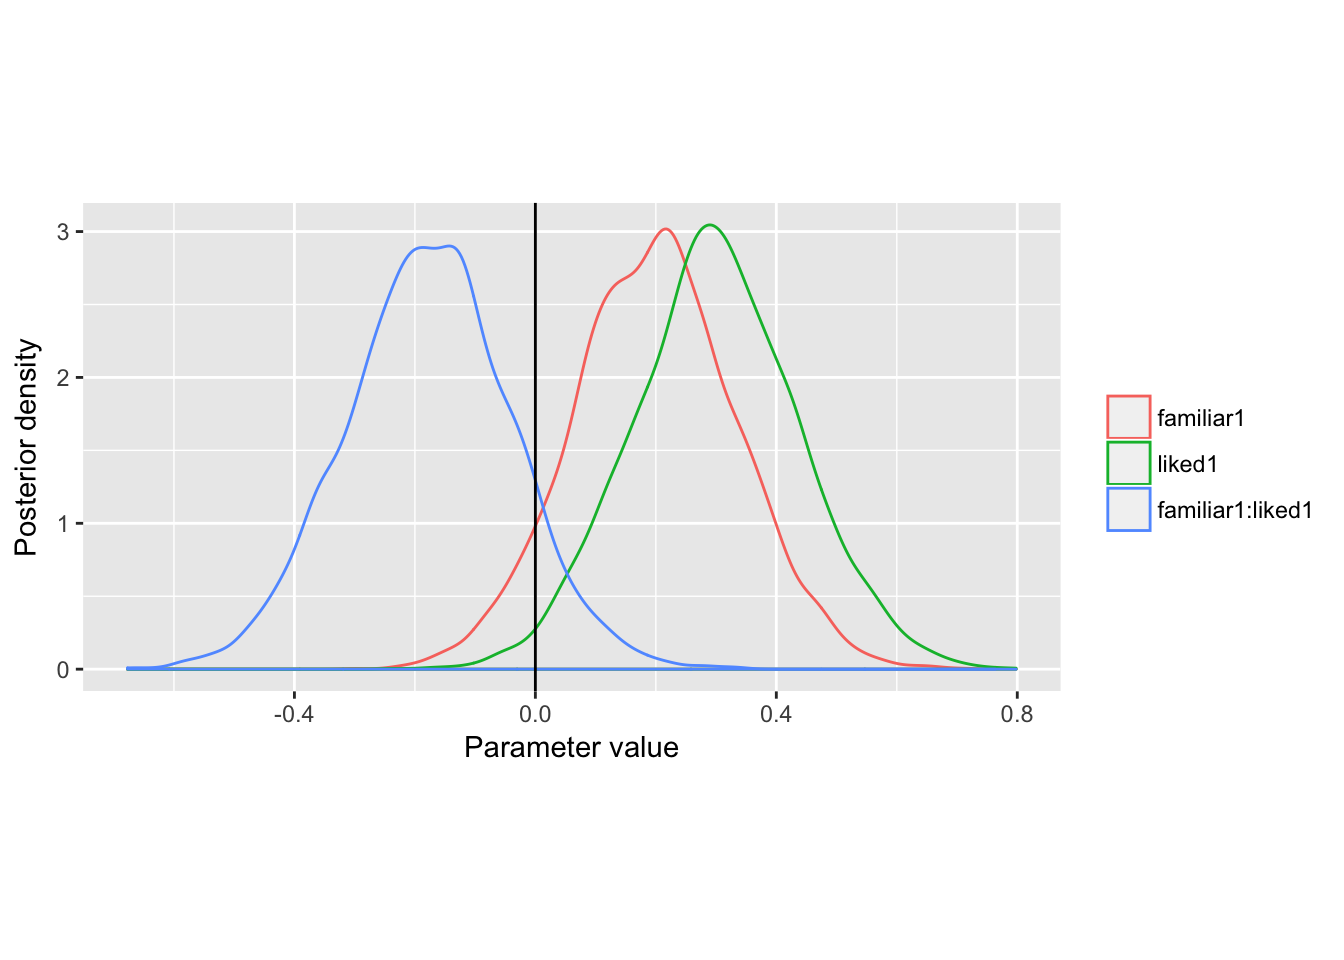
\includegraphics{packages_files/figure-latex/unnamed-chunk-5-1.pdf}

The rule is to type \texttt{package::function(parameters)}, where \texttt{::} separates the
package and function names. Parameters are just the inputs to the function.

There are two reasons not to load a package before using it:

\begin{enumerate}
\def\labelenumi{\arabic{enumi}.}
\item
  Laziness: it can save typing if you just want to use one function from a
  package, and only once.
\item
  Explicitness: It's an unfortunate truth that some function names are repeated
  in different packages. This can be confusing if they work differently or do
  comepletely different things. If you don't know which package the version you
  are using comes from. Using \texttt{package\_name:function\_name} can help make things
  explicit.
\end{enumerate}

Try using the \texttt{hist.data.frame} function in the \texttt{Hmisc} package on the \texttt{mtcars}
data.

\begin{itemize}
\tightlist
\item
  First using the \texttt{::} syntax
\item
  Then load the \texttt{Hmisc} package, and repeat without using the \texttt{::}.
\end{itemize}

\hypertarget{data}{%
\part{Data}\label{data}}

\hypertarget{datasets-dataframes}{%
\section{\texorpdfstring{The \texttt{dataframe}}{The dataframe}}\label{datasets-dataframes}}

A \texttt{dataframe} is a container for our data.

It's much like a spreadsheet, but with some constraints applied. `Constraints'
might sound bad, but they're actually helpful: they make dataframes more
structured and predictable to work with. The main constraints are that:

\begin{itemize}
\item
  Each column is a \protect\hyperlink{vectors-and-lists}{vector}, and so can
  \protect\hyperlink{vectors-and-lists}{only store one type of data}.
\item
  Every column has to be the same length (although missing values are
  allowed).
\item
  Each column must have a name.
\end{itemize}

A \texttt{tibble} is an updated version of a dataframe with a whimsical name, which is
part of the \texttt{tidyverse}. It's almost exactly the same a dataframe, but with some
rough edges smoothed off --- it's safe and preferred to use \texttt{tibble} in place of
\texttt{data.frame}.

You can make a simple tibble or dataframe like this:

\begin{Shaded}
\begin{Highlighting}[]
\KeywordTok{data.frame}\NormalTok{(}\DataTypeTok{myvariable =} \DecValTok{1}\OperatorTok{:}\DecValTok{10}\NormalTok{)}
\NormalTok{   myvariable}
\DecValTok{1}           \DecValTok{1}
\DecValTok{2}           \DecValTok{2}
\DecValTok{3}           \DecValTok{3}
\DecValTok{4}           \DecValTok{4}
\DecValTok{5}           \DecValTok{5}
\DecValTok{6}           \DecValTok{6}
\DecValTok{7}           \DecValTok{7}
\DecValTok{8}           \DecValTok{8}
\DecValTok{9}           \DecValTok{9}
\DecValTok{10}         \DecValTok{10}
\end{Highlighting}
\end{Shaded}

Using a tible is much the same, but allows some extra tricks like creating one
variable from another:

\begin{Shaded}
\begin{Highlighting}[]
\KeywordTok{tibble}\NormalTok{(}
    \DataTypeTok{height_m =} \KeywordTok{rnorm}\NormalTok{(}\DecValTok{10}\NormalTok{, }\FloatTok{1.5}\NormalTok{, }\FloatTok{.2}\NormalTok{),}
    \DataTypeTok{weight_kg =} \KeywordTok{rnorm}\NormalTok{(}\DecValTok{10}\NormalTok{, }\DecValTok{65}\NormalTok{, }\DecValTok{10}\NormalTok{),}
    \DataTypeTok{bmi =}\NormalTok{ weight_kg }\OperatorTok{/}\StringTok{ }\NormalTok{height_m }\OperatorTok{^}\StringTok{ }\DecValTok{2}\NormalTok{,}
    \DataTypeTok{overweight =}\NormalTok{ bmi }\OperatorTok{>}\StringTok{ }\DecValTok{25}
\NormalTok{)}
\CommentTok{# A tibble: 10 x 4}
\NormalTok{   height_m weight_kg   bmi overweight}
      \OperatorTok{<}\NormalTok{dbl}\OperatorTok{>}\StringTok{     }\ErrorTok{<}\NormalTok{dbl}\OperatorTok{>}\StringTok{ }\ErrorTok{<}\NormalTok{dbl}\OperatorTok{>}\StringTok{ }\ErrorTok{<}\NormalTok{lgl}\OperatorTok{>}\StringTok{     }
\StringTok{ }\DecValTok{1}     \FloatTok{1.18}      \FloatTok{55.8}  \FloatTok{40.2} \OtherTok{TRUE}      
 \DecValTok{2}     \FloatTok{1.30}      \FloatTok{57.5}  \FloatTok{34.0} \OtherTok{TRUE}      
 \DecValTok{3}     \FloatTok{1.65}      \FloatTok{74.7}  \FloatTok{27.6} \OtherTok{TRUE}      
 \DecValTok{4}     \FloatTok{1.51}      \FloatTok{48.0}  \FloatTok{20.9} \OtherTok{FALSE}     
 \DecValTok{5}     \FloatTok{1.61}      \FloatTok{61.2}  \FloatTok{23.7} \OtherTok{FALSE}     
 \DecValTok{6}     \FloatTok{1.20}      \FloatTok{65.8}  \FloatTok{45.9} \OtherTok{TRUE}      
 \DecValTok{7}     \FloatTok{1.49}      \FloatTok{52.5}  \FloatTok{23.7} \OtherTok{FALSE}     
 \DecValTok{8}     \FloatTok{1.81}      \FloatTok{63.7}  \FloatTok{19.5} \OtherTok{FALSE}     
 \DecValTok{9}     \FloatTok{1.55}      \FloatTok{66.0}  \FloatTok{27.6} \OtherTok{TRUE}      
\DecValTok{10}     \FloatTok{1.45}      \FloatTok{57.3}  \FloatTok{27.4} \OtherTok{TRUE}      
\end{Highlighting}
\end{Shaded}

\hypertarget{built-in-data}{%
\paragraph{Using `built in' data}\label{built-in-data}}
\addcontentsline{toc}{paragraph}{Using `built in' data}

The quickest way to see a dataframe in action is to use one that is built in to
R
(\href{https://stat.ethz.ch/R-manual/R-devel/library/datasets/html/00Index.html}{this page}
lists all the built-in datasets). For example:

\begin{Shaded}
\begin{Highlighting}[]
\KeywordTok{head}\NormalTok{(airquality)}
\NormalTok{  Ozone Solar.R Wind Temp Month Day}
\DecValTok{1}    \DecValTok{41}     \DecValTok{190}  \FloatTok{7.4}   \DecValTok{67}     \DecValTok{5}   \DecValTok{1}
\DecValTok{2}    \DecValTok{36}     \DecValTok{118}  \FloatTok{8.0}   \DecValTok{72}     \DecValTok{5}   \DecValTok{2}
\DecValTok{3}    \DecValTok{12}     \DecValTok{149} \FloatTok{12.6}   \DecValTok{74}     \DecValTok{5}   \DecValTok{3}
\DecValTok{4}    \DecValTok{18}     \DecValTok{313} \FloatTok{11.5}   \DecValTok{62}     \DecValTok{5}   \DecValTok{4}
\DecValTok{5}    \OtherTok{NA}      \OtherTok{NA} \FloatTok{14.3}   \DecValTok{56}     \DecValTok{5}   \DecValTok{5}
\DecValTok{6}    \DecValTok{28}      \OtherTok{NA} \FloatTok{14.9}   \DecValTok{66}     \DecValTok{5}   \DecValTok{6}
\end{Highlighting}
\end{Shaded}

Or

\begin{Shaded}
\begin{Highlighting}[]
\KeywordTok{head}\NormalTok{(mtcars)}
\NormalTok{                   mpg cyl disp  hp drat    wt  qsec vs am gear carb}
\NormalTok{Mazda RX4         }\FloatTok{21.0}   \DecValTok{6}  \DecValTok{160} \DecValTok{110} \FloatTok{3.90} \FloatTok{2.620} \FloatTok{16.46}  \DecValTok{0}  \DecValTok{1}    \DecValTok{4}    \DecValTok{4}
\NormalTok{Mazda RX4 Wag     }\FloatTok{21.0}   \DecValTok{6}  \DecValTok{160} \DecValTok{110} \FloatTok{3.90} \FloatTok{2.875} \FloatTok{17.02}  \DecValTok{0}  \DecValTok{1}    \DecValTok{4}    \DecValTok{4}
\NormalTok{Datsun }\DecValTok{710}        \FloatTok{22.8}   \DecValTok{4}  \DecValTok{108}  \DecValTok{93} \FloatTok{3.85} \FloatTok{2.320} \FloatTok{18.61}  \DecValTok{1}  \DecValTok{1}    \DecValTok{4}    \DecValTok{1}
\NormalTok{Hornet }\DecValTok{4}\NormalTok{ Drive    }\FloatTok{21.4}   \DecValTok{6}  \DecValTok{258} \DecValTok{110} \FloatTok{3.08} \FloatTok{3.215} \FloatTok{19.44}  \DecValTok{1}  \DecValTok{0}    \DecValTok{3}    \DecValTok{1}
\NormalTok{Hornet Sportabout }\FloatTok{18.7}   \DecValTok{8}  \DecValTok{360} \DecValTok{175} \FloatTok{3.15} \FloatTok{3.440} \FloatTok{17.02}  \DecValTok{0}  \DecValTok{0}    \DecValTok{3}    \DecValTok{2}
\NormalTok{Valiant           }\FloatTok{18.1}   \DecValTok{6}  \DecValTok{225} \DecValTok{105} \FloatTok{2.76} \FloatTok{3.460} \FloatTok{20.22}  \DecValTok{1}  \DecValTok{0}    \DecValTok{3}    \DecValTok{1}
\end{Highlighting}
\end{Shaded}

In both these examples the datasets are already loaded and available to be used
with the \texttt{head()} function.

To find a list of all the built in datasets you can type \texttt{help(datasets)} into
the console, or see
\url{https://stat.ethz.ch/R-manual/R-devel/library/datasets/html/00Index.html}.

Familiarise yourself with some of the other included datasets, e.g.
\texttt{datasets::attitude}. Watch out that not all the included datasets are
\emph{dataframes}: Some are just vectors of observations (e.g.~the \texttt{airmiles} data)
and some are `time-series', (e.g.~the \texttt{co2} data)

\hypertarget{looking-at-data}{%
\paragraph{Looking at dataframes}\label{looking-at-data}}
\addcontentsline{toc}{paragraph}{Looking at dataframes}

As we've already seen, using \texttt{print(df)} within an RMarkdown document creates a
nice interactive table you can use to look at your data.

However you won't want to print your whole data file when you Knit your
RMarkdown document. The \texttt{head} function can be useful if you just want to show a
few rows:

\begin{Shaded}
\begin{Highlighting}[]
\KeywordTok{head}\NormalTok{(mtcars)}
\NormalTok{                   mpg cyl disp  hp drat    wt  qsec vs am gear carb}
\NormalTok{Mazda RX4         }\FloatTok{21.0}   \DecValTok{6}  \DecValTok{160} \DecValTok{110} \FloatTok{3.90} \FloatTok{2.620} \FloatTok{16.46}  \DecValTok{0}  \DecValTok{1}    \DecValTok{4}    \DecValTok{4}
\NormalTok{Mazda RX4 Wag     }\FloatTok{21.0}   \DecValTok{6}  \DecValTok{160} \DecValTok{110} \FloatTok{3.90} \FloatTok{2.875} \FloatTok{17.02}  \DecValTok{0}  \DecValTok{1}    \DecValTok{4}    \DecValTok{4}
\NormalTok{Datsun }\DecValTok{710}        \FloatTok{22.8}   \DecValTok{4}  \DecValTok{108}  \DecValTok{93} \FloatTok{3.85} \FloatTok{2.320} \FloatTok{18.61}  \DecValTok{1}  \DecValTok{1}    \DecValTok{4}    \DecValTok{1}
\NormalTok{Hornet }\DecValTok{4}\NormalTok{ Drive    }\FloatTok{21.4}   \DecValTok{6}  \DecValTok{258} \DecValTok{110} \FloatTok{3.08} \FloatTok{3.215} \FloatTok{19.44}  \DecValTok{1}  \DecValTok{0}    \DecValTok{3}    \DecValTok{1}
\NormalTok{Hornet Sportabout }\FloatTok{18.7}   \DecValTok{8}  \DecValTok{360} \DecValTok{175} \FloatTok{3.15} \FloatTok{3.440} \FloatTok{17.02}  \DecValTok{0}  \DecValTok{0}    \DecValTok{3}    \DecValTok{2}
\NormalTok{Valiant           }\FloatTok{18.1}   \DecValTok{6}  \DecValTok{225} \DecValTok{105} \FloatTok{2.76} \FloatTok{3.460} \FloatTok{20.22}  \DecValTok{1}  \DecValTok{0}    \DecValTok{3}    \DecValTok{1}
\end{Highlighting}
\end{Shaded}

Or we can use \texttt{glimpse()} function from the \texttt{dplyr::} package (see the
\protect\hyperlink{packages}{section on loading and using packages}) for a different view of the
first few rows of the \texttt{mtcars} data. This flips the dataframe so the variables
are listed in the first column of the output:

\begin{Shaded}
\begin{Highlighting}[]
\KeywordTok{glimpse}\NormalTok{(mtcars)}
\NormalTok{Observations}\OperatorTok{:}\StringTok{ }\DecValTok{32}
\NormalTok{Variables}\OperatorTok{:}\StringTok{ }\DecValTok{11}
\OperatorTok{$}\StringTok{ }\NormalTok{mpg  }\OperatorTok{<}\NormalTok{dbl}\OperatorTok{>}\StringTok{ }\FloatTok{21.0}\NormalTok{, }\FloatTok{21.0}\NormalTok{, }\FloatTok{22.8}\NormalTok{, }\FloatTok{21.4}\NormalTok{, }\FloatTok{18.7}\NormalTok{, }\FloatTok{18.1}\NormalTok{, }\FloatTok{14.3}\NormalTok{, }\FloatTok{24.4}\NormalTok{, }\FloatTok{22.8}\NormalTok{, }\DecValTok{19}\NormalTok{....}
\OperatorTok{$}\StringTok{ }\NormalTok{cyl  }\OperatorTok{<}\NormalTok{dbl}\OperatorTok{>}\StringTok{ }\DecValTok{6}\NormalTok{, }\DecValTok{6}\NormalTok{, }\DecValTok{4}\NormalTok{, }\DecValTok{6}\NormalTok{, }\DecValTok{8}\NormalTok{, }\DecValTok{6}\NormalTok{, }\DecValTok{8}\NormalTok{, }\DecValTok{4}\NormalTok{, }\DecValTok{4}\NormalTok{, }\DecValTok{6}\NormalTok{, }\DecValTok{6}\NormalTok{, }\DecValTok{8}\NormalTok{, }\DecValTok{8}\NormalTok{, }\DecValTok{8}\NormalTok{, }\DecValTok{8}\NormalTok{, }\DecValTok{8}\NormalTok{, }\DecValTok{8}\NormalTok{, }\DecValTok{4}\NormalTok{, }\DecValTok{4}\NormalTok{, ...}
\OperatorTok{$}\StringTok{ }\NormalTok{disp }\OperatorTok{<}\NormalTok{dbl}\OperatorTok{>}\StringTok{ }\FloatTok{160.0}\NormalTok{, }\FloatTok{160.0}\NormalTok{, }\FloatTok{108.0}\NormalTok{, }\FloatTok{258.0}\NormalTok{, }\FloatTok{360.0}\NormalTok{, }\FloatTok{225.0}\NormalTok{, }\FloatTok{360.0}\NormalTok{, }\FloatTok{146.7}\NormalTok{, }\DecValTok{1}\NormalTok{...}
\OperatorTok{$}\StringTok{ }\NormalTok{hp   }\OperatorTok{<}\NormalTok{dbl}\OperatorTok{>}\StringTok{ }\DecValTok{110}\NormalTok{, }\DecValTok{110}\NormalTok{, }\DecValTok{93}\NormalTok{, }\DecValTok{110}\NormalTok{, }\DecValTok{175}\NormalTok{, }\DecValTok{105}\NormalTok{, }\DecValTok{245}\NormalTok{, }\DecValTok{62}\NormalTok{, }\DecValTok{95}\NormalTok{, }\DecValTok{123}\NormalTok{, }\DecValTok{123}\NormalTok{, }\DecValTok{180}\NormalTok{, ...}
\OperatorTok{$}\StringTok{ }\NormalTok{drat }\OperatorTok{<}\NormalTok{dbl}\OperatorTok{>}\StringTok{ }\FloatTok{3.90}\NormalTok{, }\FloatTok{3.90}\NormalTok{, }\FloatTok{3.85}\NormalTok{, }\FloatTok{3.08}\NormalTok{, }\FloatTok{3.15}\NormalTok{, }\FloatTok{2.76}\NormalTok{, }\FloatTok{3.21}\NormalTok{, }\FloatTok{3.69}\NormalTok{, }\FloatTok{3.92}\NormalTok{, }\DecValTok{3}\NormalTok{.}\DecValTok{9}\NormalTok{...}
\OperatorTok{$}\StringTok{ }\NormalTok{wt   }\OperatorTok{<}\NormalTok{dbl}\OperatorTok{>}\StringTok{ }\FloatTok{2.620}\NormalTok{, }\FloatTok{2.875}\NormalTok{, }\FloatTok{2.320}\NormalTok{, }\FloatTok{3.215}\NormalTok{, }\FloatTok{3.440}\NormalTok{, }\FloatTok{3.460}\NormalTok{, }\FloatTok{3.570}\NormalTok{, }\FloatTok{3.190}\NormalTok{, }\DecValTok{3}\NormalTok{...}
\OperatorTok{$}\StringTok{ }\NormalTok{qsec }\OperatorTok{<}\NormalTok{dbl}\OperatorTok{>}\StringTok{ }\FloatTok{16.46}\NormalTok{, }\FloatTok{17.02}\NormalTok{, }\FloatTok{18.61}\NormalTok{, }\FloatTok{19.44}\NormalTok{, }\FloatTok{17.02}\NormalTok{, }\FloatTok{20.22}\NormalTok{, }\FloatTok{15.84}\NormalTok{, }\FloatTok{20.00}\NormalTok{, }\DecValTok{2}\NormalTok{...}
\OperatorTok{$}\StringTok{ }\NormalTok{vs   }\OperatorTok{<}\NormalTok{dbl}\OperatorTok{>}\StringTok{ }\DecValTok{0}\NormalTok{, }\DecValTok{0}\NormalTok{, }\DecValTok{1}\NormalTok{, }\DecValTok{1}\NormalTok{, }\DecValTok{0}\NormalTok{, }\DecValTok{1}\NormalTok{, }\DecValTok{0}\NormalTok{, }\DecValTok{1}\NormalTok{, }\DecValTok{1}\NormalTok{, }\DecValTok{1}\NormalTok{, }\DecValTok{1}\NormalTok{, }\DecValTok{0}\NormalTok{, }\DecValTok{0}\NormalTok{, }\DecValTok{0}\NormalTok{, }\DecValTok{0}\NormalTok{, }\DecValTok{0}\NormalTok{, }\DecValTok{0}\NormalTok{, }\DecValTok{1}\NormalTok{, }\DecValTok{1}\NormalTok{, ...}
\OperatorTok{$}\StringTok{ }\NormalTok{am   }\OperatorTok{<}\NormalTok{dbl}\OperatorTok{>}\StringTok{ }\DecValTok{1}\NormalTok{, }\DecValTok{1}\NormalTok{, }\DecValTok{1}\NormalTok{, }\DecValTok{0}\NormalTok{, }\DecValTok{0}\NormalTok{, }\DecValTok{0}\NormalTok{, }\DecValTok{0}\NormalTok{, }\DecValTok{0}\NormalTok{, }\DecValTok{0}\NormalTok{, }\DecValTok{0}\NormalTok{, }\DecValTok{0}\NormalTok{, }\DecValTok{0}\NormalTok{, }\DecValTok{0}\NormalTok{, }\DecValTok{0}\NormalTok{, }\DecValTok{0}\NormalTok{, }\DecValTok{0}\NormalTok{, }\DecValTok{0}\NormalTok{, }\DecValTok{1}\NormalTok{, }\DecValTok{1}\NormalTok{, ...}
\OperatorTok{$}\StringTok{ }\NormalTok{gear }\OperatorTok{<}\NormalTok{dbl}\OperatorTok{>}\StringTok{ }\DecValTok{4}\NormalTok{, }\DecValTok{4}\NormalTok{, }\DecValTok{4}\NormalTok{, }\DecValTok{3}\NormalTok{, }\DecValTok{3}\NormalTok{, }\DecValTok{3}\NormalTok{, }\DecValTok{3}\NormalTok{, }\DecValTok{4}\NormalTok{, }\DecValTok{4}\NormalTok{, }\DecValTok{4}\NormalTok{, }\DecValTok{4}\NormalTok{, }\DecValTok{3}\NormalTok{, }\DecValTok{3}\NormalTok{, }\DecValTok{3}\NormalTok{, }\DecValTok{3}\NormalTok{, }\DecValTok{3}\NormalTok{, }\DecValTok{3}\NormalTok{, }\DecValTok{4}\NormalTok{, }\DecValTok{4}\NormalTok{, ...}
\OperatorTok{$}\StringTok{ }\NormalTok{carb }\OperatorTok{<}\NormalTok{dbl}\OperatorTok{>}\StringTok{ }\DecValTok{4}\NormalTok{, }\DecValTok{4}\NormalTok{, }\DecValTok{1}\NormalTok{, }\DecValTok{1}\NormalTok{, }\DecValTok{2}\NormalTok{, }\DecValTok{1}\NormalTok{, }\DecValTok{4}\NormalTok{, }\DecValTok{2}\NormalTok{, }\DecValTok{2}\NormalTok{, }\DecValTok{4}\NormalTok{, }\DecValTok{4}\NormalTok{, }\DecValTok{3}\NormalTok{, }\DecValTok{3}\NormalTok{, }\DecValTok{3}\NormalTok{, }\DecValTok{4}\NormalTok{, }\DecValTok{4}\NormalTok{, }\DecValTok{4}\NormalTok{, }\DecValTok{1}\NormalTok{, }\DecValTok{2}\NormalTok{, ...}
\end{Highlighting}
\end{Shaded}

You can use the \texttt{pander()} function (from the \texttt{pander::} package) to format
tables nicely, for when you Knit a document to HTML, Word or PDF. For example:

\begin{Shaded}
\begin{Highlighting}[]
\KeywordTok{library}\NormalTok{(pander)}
\KeywordTok{pander}\NormalTok{(}\KeywordTok{head}\NormalTok{(airquality), }\DataTypeTok{caption=}\StringTok{"Tables always need a caption."}\NormalTok{)}
\end{Highlighting}
\end{Shaded}

\begin{longtable}[]{@{}cccccc@{}}
\caption{Tables always need a caption.}\tabularnewline
\toprule
\begin{minipage}[b]{0.09\columnwidth}\centering
Ozone\strut
\end{minipage} & \begin{minipage}[b]{0.12\columnwidth}\centering
Solar.R\strut
\end{minipage} & \begin{minipage}[b]{0.08\columnwidth}\centering
Wind\strut
\end{minipage} & \begin{minipage}[b]{0.08\columnwidth}\centering
Temp\strut
\end{minipage} & \begin{minipage}[b]{0.09\columnwidth}\centering
Month\strut
\end{minipage} & \begin{minipage}[b]{0.09\columnwidth}\centering
Day\strut
\end{minipage}\tabularnewline
\midrule
\endfirsthead
\toprule
\begin{minipage}[b]{0.09\columnwidth}\centering
Ozone\strut
\end{minipage} & \begin{minipage}[b]{0.12\columnwidth}\centering
Solar.R\strut
\end{minipage} & \begin{minipage}[b]{0.08\columnwidth}\centering
Wind\strut
\end{minipage} & \begin{minipage}[b]{0.08\columnwidth}\centering
Temp\strut
\end{minipage} & \begin{minipage}[b]{0.09\columnwidth}\centering
Month\strut
\end{minipage} & \begin{minipage}[b]{0.09\columnwidth}\centering
Day\strut
\end{minipage}\tabularnewline
\midrule
\endhead
\begin{minipage}[t]{0.09\columnwidth}\centering
41\strut
\end{minipage} & \begin{minipage}[t]{0.12\columnwidth}\centering
190\strut
\end{minipage} & \begin{minipage}[t]{0.08\columnwidth}\centering
7.4\strut
\end{minipage} & \begin{minipage}[t]{0.08\columnwidth}\centering
67\strut
\end{minipage} & \begin{minipage}[t]{0.09\columnwidth}\centering
5\strut
\end{minipage} & \begin{minipage}[t]{0.09\columnwidth}\centering
1\strut
\end{minipage}\tabularnewline
\begin{minipage}[t]{0.09\columnwidth}\centering
36\strut
\end{minipage} & \begin{minipage}[t]{0.12\columnwidth}\centering
118\strut
\end{minipage} & \begin{minipage}[t]{0.08\columnwidth}\centering
8\strut
\end{minipage} & \begin{minipage}[t]{0.08\columnwidth}\centering
72\strut
\end{minipage} & \begin{minipage}[t]{0.09\columnwidth}\centering
5\strut
\end{minipage} & \begin{minipage}[t]{0.09\columnwidth}\centering
2\strut
\end{minipage}\tabularnewline
\begin{minipage}[t]{0.09\columnwidth}\centering
12\strut
\end{minipage} & \begin{minipage}[t]{0.12\columnwidth}\centering
149\strut
\end{minipage} & \begin{minipage}[t]{0.08\columnwidth}\centering
12.6\strut
\end{minipage} & \begin{minipage}[t]{0.08\columnwidth}\centering
74\strut
\end{minipage} & \begin{minipage}[t]{0.09\columnwidth}\centering
5\strut
\end{minipage} & \begin{minipage}[t]{0.09\columnwidth}\centering
3\strut
\end{minipage}\tabularnewline
\begin{minipage}[t]{0.09\columnwidth}\centering
18\strut
\end{minipage} & \begin{minipage}[t]{0.12\columnwidth}\centering
313\strut
\end{minipage} & \begin{minipage}[t]{0.08\columnwidth}\centering
11.5\strut
\end{minipage} & \begin{minipage}[t]{0.08\columnwidth}\centering
62\strut
\end{minipage} & \begin{minipage}[t]{0.09\columnwidth}\centering
5\strut
\end{minipage} & \begin{minipage}[t]{0.09\columnwidth}\centering
4\strut
\end{minipage}\tabularnewline
\begin{minipage}[t]{0.09\columnwidth}\centering
NA\strut
\end{minipage} & \begin{minipage}[t]{0.12\columnwidth}\centering
NA\strut
\end{minipage} & \begin{minipage}[t]{0.08\columnwidth}\centering
14.3\strut
\end{minipage} & \begin{minipage}[t]{0.08\columnwidth}\centering
56\strut
\end{minipage} & \begin{minipage}[t]{0.09\columnwidth}\centering
5\strut
\end{minipage} & \begin{minipage}[t]{0.09\columnwidth}\centering
5\strut
\end{minipage}\tabularnewline
\begin{minipage}[t]{0.09\columnwidth}\centering
28\strut
\end{minipage} & \begin{minipage}[t]{0.12\columnwidth}\centering
NA\strut
\end{minipage} & \begin{minipage}[t]{0.08\columnwidth}\centering
14.9\strut
\end{minipage} & \begin{minipage}[t]{0.08\columnwidth}\centering
66\strut
\end{minipage} & \begin{minipage}[t]{0.09\columnwidth}\centering
5\strut
\end{minipage} & \begin{minipage}[t]{0.09\columnwidth}\centering
6\strut
\end{minipage}\tabularnewline
\bottomrule
\end{longtable}

See the section on \protect\hyperlink{sharing-and-publication}{sharing and publishing} for more
ways to format and present tables.

Other useful functions for looking at and exploring datasets include:

\begin{itemize}
\tightlist
\item
  \texttt{summary(df)}
\item
  \texttt{psych::describe(df)}
\item
  \texttt{skimr::skim(df)}
\end{itemize}

Experiment with a few of the functions for viewing/summarising dataframes.

There are also some helpful plotting functions which accept a whole dataframe as
their input:

\begin{Shaded}
\begin{Highlighting}[]
\KeywordTok{boxplot}\NormalTok{(airquality)}
\end{Highlighting}
\end{Shaded}

\begin{figure}
\centering
\includegraphics{DATASETS_files/figure-latex/unnamed-chunk-10-1.pdf}
\caption{\label{fig:unnamed-chunk-10}Box plot of all variables in a dataset.}
\end{figure}

\begin{Shaded}
\begin{Highlighting}[]
\NormalTok{psych}\OperatorTok{::}\KeywordTok{cor.plot}\NormalTok{(airquality)}
\end{Highlighting}
\end{Shaded}

\begin{figure}
\centering
\includegraphics{DATASETS_files/figure-latex/unnamed-chunk-11-1.pdf}
\caption{\label{fig:unnamed-chunk-11}Correlation heatmap of all variables in a dataset. Colours indicate size of the correlation between pairs of variables.}
\end{figure}

These plots might not be worth including in a final write-up, but are very
useful when exploring your data.

\hypertarget{working-with-dataframes}{%
\subsection*{Working with dataframes}\label{working-with-dataframes}}
\addcontentsline{toc}{subsection}{Working with dataframes}

\hypertarget{tidyverse}{%
\subsubsection*{\texorpdfstring{Introducing the \texttt{tidyverse}}{Introducing the tidyverse}}\label{tidyverse}}
\addcontentsline{toc}{subsubsection}{Introducing the \texttt{tidyverse}}

This guide deliberately ignores many common patterns for working with
dataframes.

There are plenty of other guides for working in these older ways, but for
beginners, these techniques can be confusing. The approach shown here is based
only on functions in \protect\hyperlink{tidyverse}{the \texttt{tidyverse}}. Although simple --- and easy
to read --- the approach is extremely flexible and covers almost all of the
cases you will encounter when working with psychological data.

Specifically, we make extensive use of two tidyverse packages:

\begin{itemize}
\tightlist
\item
  \texttt{dplyr}: to select, filter and summarise data
\item
  \texttt{ggplot2}: to make plots
\end{itemize}

To load the tidyverse first write:

\begin{Shaded}
\begin{Highlighting}[]
\KeywordTok{library}\NormalTok{(tidyverse)}
\end{Highlighting}
\end{Shaded}

This can either be typed into the console or (better) included at the top of an
markdown file.

\hypertarget{selecting-columns}{%
\subsection*{Selecting columns}\label{selecting-columns}}
\addcontentsline{toc}{subsection}{Selecting columns}

To pick out single or multiple columns use the \texttt{select()} function.

The \texttt{select()} function expects a dataframe as it's first input (`argument', in
R language), followed by the names of the columns you want to extract with a
comma between each name.

It returns a \emph{new} dataframe with just those columns, in the order you
specified:

\begin{Shaded}
\begin{Highlighting}[]
\KeywordTok{head}\NormalTok{(}
  \KeywordTok{select}\NormalTok{(mtcars, cyl, hp)}
\NormalTok{)}
\NormalTok{                  cyl  hp}
\NormalTok{Mazda RX4           }\DecValTok{6} \DecValTok{110}
\NormalTok{Mazda RX4 Wag       }\DecValTok{6} \DecValTok{110}
\NormalTok{Datsun }\DecValTok{710}          \DecValTok{4}  \DecValTok{93}
\NormalTok{Hornet }\DecValTok{4}\NormalTok{ Drive      }\DecValTok{6} \DecValTok{110}
\NormalTok{Hornet Sportabout   }\DecValTok{8} \DecValTok{175}
\NormalTok{Valiant             }\DecValTok{6} \DecValTok{105}
\end{Highlighting}
\end{Shaded}

\hypertarget{saving-a-subset-of-the-data}{%
\paragraph{Saving a subset of the data}\label{saving-a-subset-of-the-data}}
\addcontentsline{toc}{paragraph}{Saving a subset of the data}

Because \texttt{dplyr} functions return a \emph{new} dataframe, we can assign the results to
a variable:

\begin{Shaded}
\begin{Highlighting}[]
\NormalTok{justcylandweight <-}\StringTok{ }\KeywordTok{select}\NormalTok{(mtcars, cyl, wt)}
\KeywordTok{summary}\NormalTok{(justcylandweight)}
\NormalTok{      cyl              wt       }
\NormalTok{ Min.   }\OperatorTok{:}\FloatTok{4.000}\NormalTok{   Min.   }\OperatorTok{:}\FloatTok{1.513}  
\NormalTok{ 1st Qu.}\OperatorTok{:}\FloatTok{4.000}\NormalTok{   1st Qu.}\OperatorTok{:}\FloatTok{2.581}  
\NormalTok{ Median }\OperatorTok{:}\FloatTok{6.000}\NormalTok{   Median }\OperatorTok{:}\FloatTok{3.325}  
\NormalTok{ Mean   }\OperatorTok{:}\FloatTok{6.188}\NormalTok{   Mean   }\OperatorTok{:}\FloatTok{3.217}  
\NormalTok{ 3rd Qu.}\OperatorTok{:}\FloatTok{8.000}\NormalTok{   3rd Qu.}\OperatorTok{:}\FloatTok{3.610}  
\NormalTok{ Max.   }\OperatorTok{:}\FloatTok{8.000}\NormalTok{   Max.   }\OperatorTok{:}\FloatTok{5.424}  
\end{Highlighting}
\end{Shaded}

\hypertarget{excluding-columns}{%
\paragraph{Excluding columns}\label{excluding-columns}}
\addcontentsline{toc}{paragraph}{Excluding columns}

If you want to keep most of the columns --- perhaps you just want to get rid of
one and keep the rest --- put a minus (\texttt{-}) sign in front of the name of the
column to drop. This then selects everything \emph{except} the column you named:

\begin{Shaded}
\begin{Highlighting}[]
\CommentTok{# Note we are just dropping the Ozone column}
\KeywordTok{head}\NormalTok{(}\KeywordTok{select}\NormalTok{(airquality, }\OperatorTok{-}\NormalTok{Ozone))}
\NormalTok{  Solar.R Wind Temp Month Day}
\DecValTok{1}     \DecValTok{190}  \FloatTok{7.4}   \DecValTok{67}     \DecValTok{5}   \DecValTok{1}
\DecValTok{2}     \DecValTok{118}  \FloatTok{8.0}   \DecValTok{72}     \DecValTok{5}   \DecValTok{2}
\DecValTok{3}     \DecValTok{149} \FloatTok{12.6}   \DecValTok{74}     \DecValTok{5}   \DecValTok{3}
\DecValTok{4}     \DecValTok{313} \FloatTok{11.5}   \DecValTok{62}     \DecValTok{5}   \DecValTok{4}
\DecValTok{5}      \OtherTok{NA} \FloatTok{14.3}   \DecValTok{56}     \DecValTok{5}   \DecValTok{5}
\DecValTok{6}      \OtherTok{NA} \FloatTok{14.9}   \DecValTok{66}     \DecValTok{5}   \DecValTok{6}
\end{Highlighting}
\end{Shaded}

\hypertarget{matching-specific-columns}{%
\paragraph{Matching specific columns}\label{matching-specific-columns}}
\addcontentsline{toc}{paragraph}{Matching specific columns}

You can use a patterns to match a subset of the columns you want. For example,
here we select all the columns where the name contains the letter \texttt{d}:

\begin{Shaded}
\begin{Highlighting}[]
\KeywordTok{head}\NormalTok{(}\KeywordTok{select}\NormalTok{(mtcars, }\KeywordTok{contains}\NormalTok{(}\StringTok{"d"}\NormalTok{)))}
\NormalTok{                  disp drat}
\NormalTok{Mazda RX4          }\DecValTok{160} \FloatTok{3.90}
\NormalTok{Mazda RX4 Wag      }\DecValTok{160} \FloatTok{3.90}
\NormalTok{Datsun }\DecValTok{710}         \DecValTok{108} \FloatTok{3.85}
\NormalTok{Hornet }\DecValTok{4}\NormalTok{ Drive     }\DecValTok{258} \FloatTok{3.08}
\NormalTok{Hornet Sportabout  }\DecValTok{360} \FloatTok{3.15}
\NormalTok{Valiant            }\DecValTok{225} \FloatTok{2.76}
\end{Highlighting}
\end{Shaded}

And you can combine these techniques to make more complex selections:

\begin{Shaded}
\begin{Highlighting}[]
\KeywordTok{head}\NormalTok{(}\KeywordTok{select}\NormalTok{(mtcars, }\KeywordTok{contains}\NormalTok{(}\StringTok{"d"}\NormalTok{), }\OperatorTok{-}\NormalTok{drat))}
\NormalTok{                  disp}
\NormalTok{Mazda RX4          }\DecValTok{160}
\NormalTok{Mazda RX4 Wag      }\DecValTok{160}
\NormalTok{Datsun }\DecValTok{710}         \DecValTok{108}
\NormalTok{Hornet }\DecValTok{4}\NormalTok{ Drive     }\DecValTok{258}
\NormalTok{Hornet Sportabout  }\DecValTok{360}
\NormalTok{Valiant            }\DecValTok{225}
\end{Highlighting}
\end{Shaded}

\hypertarget{other-methods-of-selection}{%
\paragraph{Other methods of selection}\label{other-methods-of-selection}}
\addcontentsline{toc}{paragraph}{Other methods of selection}

As a quick reference, you can use the following `verbs' to select columns in
different ways:

\begin{itemize}
\tightlist
\item
  \texttt{starts\_with()}
\item
  \texttt{ends\_with()}
\item
  \texttt{contains()}
\item
  \texttt{everything()}
\end{itemize}

See the help files for more information (type \texttt{??dplyr::select} into the
console).

\hypertarget{selecting-rows}{%
\subsection*{Selecting rows}\label{selecting-rows}}
\addcontentsline{toc}{subsection}{Selecting rows}

To select rows from a dataframe use the \texttt{filter()} function (again from
\texttt{dplyr}).

If we only wanted to rows for 6-cylindered cars, we could write:

\begin{Shaded}
\begin{Highlighting}[]
\KeywordTok{filter}\NormalTok{(mtcars, cyl}\OperatorTok{==}\DecValTok{6}\NormalTok{)}
\NormalTok{   mpg cyl  disp  hp drat    wt  qsec vs am gear carb}
\DecValTok{1} \FloatTok{21.0}   \DecValTok{6} \FloatTok{160.0} \DecValTok{110} \FloatTok{3.90} \FloatTok{2.620} \FloatTok{16.46}  \DecValTok{0}  \DecValTok{1}    \DecValTok{4}    \DecValTok{4}
\DecValTok{2} \FloatTok{21.0}   \DecValTok{6} \FloatTok{160.0} \DecValTok{110} \FloatTok{3.90} \FloatTok{2.875} \FloatTok{17.02}  \DecValTok{0}  \DecValTok{1}    \DecValTok{4}    \DecValTok{4}
\DecValTok{3} \FloatTok{21.4}   \DecValTok{6} \FloatTok{258.0} \DecValTok{110} \FloatTok{3.08} \FloatTok{3.215} \FloatTok{19.44}  \DecValTok{1}  \DecValTok{0}    \DecValTok{3}    \DecValTok{1}
\DecValTok{4} \FloatTok{18.1}   \DecValTok{6} \FloatTok{225.0} \DecValTok{105} \FloatTok{2.76} \FloatTok{3.460} \FloatTok{20.22}  \DecValTok{1}  \DecValTok{0}    \DecValTok{3}    \DecValTok{1}
\DecValTok{5} \FloatTok{19.2}   \DecValTok{6} \FloatTok{167.6} \DecValTok{123} \FloatTok{3.92} \FloatTok{3.440} \FloatTok{18.30}  \DecValTok{1}  \DecValTok{0}    \DecValTok{4}    \DecValTok{4}
\DecValTok{6} \FloatTok{17.8}   \DecValTok{6} \FloatTok{167.6} \DecValTok{123} \FloatTok{3.92} \FloatTok{3.440} \FloatTok{18.90}  \DecValTok{1}  \DecValTok{0}    \DecValTok{4}    \DecValTok{4}
\DecValTok{7} \FloatTok{19.7}   \DecValTok{6} \FloatTok{145.0} \DecValTok{175} \FloatTok{3.62} \FloatTok{2.770} \FloatTok{15.50}  \DecValTok{0}  \DecValTok{1}    \DecValTok{5}    \DecValTok{6}
\end{Highlighting}
\end{Shaded}

\hypertarget{operators}{%
\subsection*{`Operators'}\label{operators}}
\addcontentsline{toc}{subsection}{`Operators'}

When selecting rows in the \protect\hyperlink{selecting-rows}{example above} we used two equals
signs \texttt{==} to select rows where \texttt{cyl} was exactly \texttt{6}.

As you might guess, there are other `operators' we can use to create filters.

Rather than describe them, the examples below demonstrate what each of them do.

Equality and matching

As above, to compare a single value we use \texttt{==}

\begin{Shaded}
\begin{Highlighting}[]
\DecValTok{2} \OperatorTok{==}\StringTok{ }\DecValTok{2}
\NormalTok{[}\DecValTok{1}\NormalTok{] }\OtherTok{TRUE}
\end{Highlighting}
\end{Shaded}

And in a filter:

\begin{Shaded}
\begin{Highlighting}[]
\KeywordTok{filter}\NormalTok{(mtcars, cyl}\OperatorTok{==}\DecValTok{6}\NormalTok{)}
\NormalTok{   mpg cyl  disp  hp drat    wt  qsec vs am gear carb}
\DecValTok{1} \FloatTok{21.0}   \DecValTok{6} \FloatTok{160.0} \DecValTok{110} \FloatTok{3.90} \FloatTok{2.620} \FloatTok{16.46}  \DecValTok{0}  \DecValTok{1}    \DecValTok{4}    \DecValTok{4}
\DecValTok{2} \FloatTok{21.0}   \DecValTok{6} \FloatTok{160.0} \DecValTok{110} \FloatTok{3.90} \FloatTok{2.875} \FloatTok{17.02}  \DecValTok{0}  \DecValTok{1}    \DecValTok{4}    \DecValTok{4}
\DecValTok{3} \FloatTok{21.4}   \DecValTok{6} \FloatTok{258.0} \DecValTok{110} \FloatTok{3.08} \FloatTok{3.215} \FloatTok{19.44}  \DecValTok{1}  \DecValTok{0}    \DecValTok{3}    \DecValTok{1}
\DecValTok{4} \FloatTok{18.1}   \DecValTok{6} \FloatTok{225.0} \DecValTok{105} \FloatTok{2.76} \FloatTok{3.460} \FloatTok{20.22}  \DecValTok{1}  \DecValTok{0}    \DecValTok{3}    \DecValTok{1}
\DecValTok{5} \FloatTok{19.2}   \DecValTok{6} \FloatTok{167.6} \DecValTok{123} \FloatTok{3.92} \FloatTok{3.440} \FloatTok{18.30}  \DecValTok{1}  \DecValTok{0}    \DecValTok{4}    \DecValTok{4}
\DecValTok{6} \FloatTok{17.8}   \DecValTok{6} \FloatTok{167.6} \DecValTok{123} \FloatTok{3.92} \FloatTok{3.440} \FloatTok{18.90}  \DecValTok{1}  \DecValTok{0}    \DecValTok{4}    \DecValTok{4}
\DecValTok{7} \FloatTok{19.7}   \DecValTok{6} \FloatTok{145.0} \DecValTok{175} \FloatTok{3.62} \FloatTok{2.770} \FloatTok{15.50}  \DecValTok{0}  \DecValTok{1}    \DecValTok{5}    \DecValTok{6}
\end{Highlighting}
\end{Shaded}

You might have noted above that we write \texttt{==} rather than just \texttt{=} to define the
criteria. This is because most programming languages, including R, use two \texttt{=}
symbols to distinguish: \emph{comparison} from \emph{assignment}.

Presence/absence

To test if a value is in a vector of suitable matches we can use: \texttt{\%in\%}:

\begin{Shaded}
\begin{Highlighting}[]
\DecValTok{5} \OperatorTok\StringTok{ }\DecValTok{1}\OperatorTok{:}\DecValTok{10}
\NormalTok{[}\DecValTok{1}\NormalTok{] }\OtherTok{TRUE}
\end{Highlighting}
\end{Shaded}

Or for an example which is not true:

\begin{Shaded}
\begin{Highlighting}[]
\DecValTok{100} \OperatorTok\StringTok{ }\DecValTok{1}\OperatorTok{:}\DecValTok{10}
\NormalTok{[}\DecValTok{1}\NormalTok{] }\OtherTok{FALSE}
\end{Highlighting}
\end{Shaded}

Perhaps less obviously, we can test whether each value in a vector is \emph{in} a
second vector.

This returns a vector of \texttt{TRUE/FALSE} values as long as the first list:

\begin{Shaded}
\begin{Highlighting}[]
\KeywordTok{c}\NormalTok{(}\DecValTok{1}\NormalTok{, }\DecValTok{2}\NormalTok{) }\OperatorTok\StringTok{ }\KeywordTok{c}\NormalTok{(}\DecValTok{2}\NormalTok{, }\DecValTok{3}\NormalTok{, }\DecValTok{4}\NormalTok{)}
\NormalTok{[}\DecValTok{1}\NormalTok{] }\OtherTok{FALSE}  \OtherTok{TRUE}
\end{Highlighting}
\end{Shaded}

This is very useful in a dataframe filter:

\begin{Shaded}
\begin{Highlighting}[]
\KeywordTok{head}\NormalTok{(}\KeywordTok{filter}\NormalTok{(mtcars, cyl }\OperatorTok\StringTok{ }\KeywordTok{c}\NormalTok{(}\DecValTok{4}\NormalTok{, }\DecValTok{6}\NormalTok{)))}
\NormalTok{   mpg cyl  disp  hp drat    wt  qsec vs am gear carb}
\DecValTok{1} \FloatTok{21.0}   \DecValTok{6} \FloatTok{160.0} \DecValTok{110} \FloatTok{3.90} \FloatTok{2.620} \FloatTok{16.46}  \DecValTok{0}  \DecValTok{1}    \DecValTok{4}    \DecValTok{4}
\DecValTok{2} \FloatTok{21.0}   \DecValTok{6} \FloatTok{160.0} \DecValTok{110} \FloatTok{3.90} \FloatTok{2.875} \FloatTok{17.02}  \DecValTok{0}  \DecValTok{1}    \DecValTok{4}    \DecValTok{4}
\DecValTok{3} \FloatTok{22.8}   \DecValTok{4} \FloatTok{108.0}  \DecValTok{93} \FloatTok{3.85} \FloatTok{2.320} \FloatTok{18.61}  \DecValTok{1}  \DecValTok{1}    \DecValTok{4}    \DecValTok{1}
\DecValTok{4} \FloatTok{21.4}   \DecValTok{6} \FloatTok{258.0} \DecValTok{110} \FloatTok{3.08} \FloatTok{3.215} \FloatTok{19.44}  \DecValTok{1}  \DecValTok{0}    \DecValTok{3}    \DecValTok{1}
\DecValTok{5} \FloatTok{18.1}   \DecValTok{6} \FloatTok{225.0} \DecValTok{105} \FloatTok{2.76} \FloatTok{3.460} \FloatTok{20.22}  \DecValTok{1}  \DecValTok{0}    \DecValTok{3}    \DecValTok{1}
\DecValTok{6} \FloatTok{24.4}   \DecValTok{4} \FloatTok{146.7}  \DecValTok{62} \FloatTok{3.69} \FloatTok{3.190} \FloatTok{20.00}  \DecValTok{1}  \DecValTok{0}    \DecValTok{4}    \DecValTok{2}
\end{Highlighting}
\end{Shaded}

Here we selected all rows where \texttt{cyl} matched either \texttt{4} or \texttt{6}. That is, where
the value of \texttt{cyl} was `in' the vector \texttt{c(4,6)}.

Greater/less than

The \texttt{\textless{}} and \texttt{\textgreater{}} symbols work as you'd expect:

\begin{Shaded}
\begin{Highlighting}[]
\KeywordTok{head}\NormalTok{(}\KeywordTok{filter}\NormalTok{(mtcars, cyl }\OperatorTok{>}\StringTok{ }\DecValTok{4}\NormalTok{))}
\KeywordTok{head}\NormalTok{(}\KeywordTok{filter}\NormalTok{(mtcars, cyl }\OperatorTok{<}\StringTok{ }\DecValTok{5}\NormalTok{))}
\end{Highlighting}
\end{Shaded}

You can also use \texttt{\textgreater{}=} and \texttt{\textless{}=}:

\begin{Shaded}
\begin{Highlighting}[]
\KeywordTok{filter}\NormalTok{(mtcars, cyl }\OperatorTok{>=}\StringTok{ }\DecValTok{6}\NormalTok{)}
\KeywordTok{filter}\NormalTok{(mtcars, cyl }\OperatorTok{<=}\StringTok{ }\DecValTok{4}\NormalTok{)}
\end{Highlighting}
\end{Shaded}

Negation (opposite of)

The \texttt{!} is very useful to tell R to reverse an expression; that is, take the
opposite of the value. In the simplest example:

\begin{Shaded}
\begin{Highlighting}[]
\OperatorTok{!}\OtherTok{TRUE}
\NormalTok{[}\DecValTok{1}\NormalTok{] }\OtherTok{FALSE}
\end{Highlighting}
\end{Shaded}

This is helpful because we can reverse the meaning of other expressions:

\begin{Shaded}
\begin{Highlighting}[]
\KeywordTok{is.na}\NormalTok{(}\OtherTok{NA}\NormalTok{)}
\NormalTok{[}\DecValTok{1}\NormalTok{] }\OtherTok{TRUE}
\OperatorTok{!}\KeywordTok{is.na}\NormalTok{(}\OtherTok{NA}\NormalTok{)}
\NormalTok{[}\DecValTok{1}\NormalTok{] }\OtherTok{FALSE}
\end{Highlighting}
\end{Shaded}

And we can use in dplyr filters.

Here we select rows where \texttt{Ozone} is missing (\texttt{NA}):

\begin{Shaded}
\begin{Highlighting}[]
\KeywordTok{filter}\NormalTok{(airquality, }\KeywordTok{is.na}\NormalTok{(Ozone))}
\end{Highlighting}
\end{Shaded}

And here we use \texttt{!} to reverse the expression and select rows which are not
missing:

\begin{Shaded}
\begin{Highlighting}[]
\KeywordTok{filter}\NormalTok{(airquality, }\OperatorTok{!}\KeywordTok{is.na}\NormalTok{(Ozone))}
\end{Highlighting}
\end{Shaded}

Try running these commands for yourself and experiment with changing the
operators to make select different combinations of rows

Other logical operators

There are operators for `and'/`or' which can combine other filters.

Using \texttt{\&} (and) with two condtions makes the filter more restrictive:

\begin{Shaded}
\begin{Highlighting}[]
\KeywordTok{filter}\NormalTok{(mtcars, hp }\OperatorTok{>}\StringTok{ }\DecValTok{200} \OperatorTok{&}\StringTok{ }\NormalTok{wt }\OperatorTok{>}\StringTok{ }\DecValTok{4}\NormalTok{)}
\NormalTok{   mpg cyl disp  hp drat    wt  qsec vs am gear carb}
\DecValTok{1} \FloatTok{10.4}   \DecValTok{8}  \DecValTok{472} \DecValTok{205} \FloatTok{2.93} \FloatTok{5.250} \FloatTok{17.98}  \DecValTok{0}  \DecValTok{0}    \DecValTok{3}    \DecValTok{4}
\DecValTok{2} \FloatTok{10.4}   \DecValTok{8}  \DecValTok{460} \DecValTok{215} \FloatTok{3.00} \FloatTok{5.424} \FloatTok{17.82}  \DecValTok{0}  \DecValTok{0}    \DecValTok{3}    \DecValTok{4}
\DecValTok{3} \FloatTok{14.7}   \DecValTok{8}  \DecValTok{440} \DecValTok{230} \FloatTok{3.23} \FloatTok{5.345} \FloatTok{17.42}  \DecValTok{0}  \DecValTok{0}    \DecValTok{3}    \DecValTok{4}
\end{Highlighting}
\end{Shaded}

In contrast, the pipe symbol, \texttt{\textbar{}}, means `or', so we match more rows:

\begin{Shaded}
\begin{Highlighting}[]
\KeywordTok{filter}\NormalTok{(mtcars, hp }\OperatorTok{>}\StringTok{ }\DecValTok{200} \OperatorTok{|}\StringTok{ }\NormalTok{wt }\OperatorTok{>}\StringTok{ }\DecValTok{4}\NormalTok{)}
\NormalTok{   mpg cyl  disp  hp drat    wt  qsec vs am gear carb}
\DecValTok{1} \FloatTok{14.3}   \DecValTok{8} \FloatTok{360.0} \DecValTok{245} \FloatTok{3.21} \FloatTok{3.570} \FloatTok{15.84}  \DecValTok{0}  \DecValTok{0}    \DecValTok{3}    \DecValTok{4}
\DecValTok{2} \FloatTok{16.4}   \DecValTok{8} \FloatTok{275.8} \DecValTok{180} \FloatTok{3.07} \FloatTok{4.070} \FloatTok{17.40}  \DecValTok{0}  \DecValTok{0}    \DecValTok{3}    \DecValTok{3}
\DecValTok{3} \FloatTok{10.4}   \DecValTok{8} \FloatTok{472.0} \DecValTok{205} \FloatTok{2.93} \FloatTok{5.250} \FloatTok{17.98}  \DecValTok{0}  \DecValTok{0}    \DecValTok{3}    \DecValTok{4}
\DecValTok{4} \FloatTok{10.4}   \DecValTok{8} \FloatTok{460.0} \DecValTok{215} \FloatTok{3.00} \FloatTok{5.424} \FloatTok{17.82}  \DecValTok{0}  \DecValTok{0}    \DecValTok{3}    \DecValTok{4}
\DecValTok{5} \FloatTok{14.7}   \DecValTok{8} \FloatTok{440.0} \DecValTok{230} \FloatTok{3.23} \FloatTok{5.345} \FloatTok{17.42}  \DecValTok{0}  \DecValTok{0}    \DecValTok{3}    \DecValTok{4}
\DecValTok{6} \FloatTok{13.3}   \DecValTok{8} \FloatTok{350.0} \DecValTok{245} \FloatTok{3.73} \FloatTok{3.840} \FloatTok{15.41}  \DecValTok{0}  \DecValTok{0}    \DecValTok{3}    \DecValTok{4}
\DecValTok{7} \FloatTok{15.8}   \DecValTok{8} \FloatTok{351.0} \DecValTok{264} \FloatTok{4.22} \FloatTok{3.170} \FloatTok{14.50}  \DecValTok{0}  \DecValTok{1}    \DecValTok{5}    \DecValTok{4}
\DecValTok{8} \FloatTok{15.0}   \DecValTok{8} \FloatTok{301.0} \DecValTok{335} \FloatTok{3.54} \FloatTok{3.570} \FloatTok{14.60}  \DecValTok{0}  \DecValTok{1}    \DecValTok{5}    \DecValTok{8}
\end{Highlighting}
\end{Shaded}

Finally, you can set the order in which operators are applied by using
parentheses. This means these expressions are subtly different:

\begin{Shaded}
\begin{Highlighting}[]
\CommentTok{# first}
\KeywordTok{filter}\NormalTok{(mtcars, (hp }\OperatorTok{>}\StringTok{ }\DecValTok{200} \OperatorTok{&}\StringTok{ }\NormalTok{wt }\OperatorTok{>}\StringTok{ }\DecValTok{4}\NormalTok{) }\OperatorTok{|}\StringTok{ }\NormalTok{cyl}\OperatorTok{==}\DecValTok{8}\NormalTok{)}
\NormalTok{    mpg cyl  disp  hp drat    wt  qsec vs am gear carb}
\DecValTok{1}  \FloatTok{18.7}   \DecValTok{8} \FloatTok{360.0} \DecValTok{175} \FloatTok{3.15} \FloatTok{3.440} \FloatTok{17.02}  \DecValTok{0}  \DecValTok{0}    \DecValTok{3}    \DecValTok{2}
\DecValTok{2}  \FloatTok{14.3}   \DecValTok{8} \FloatTok{360.0} \DecValTok{245} \FloatTok{3.21} \FloatTok{3.570} \FloatTok{15.84}  \DecValTok{0}  \DecValTok{0}    \DecValTok{3}    \DecValTok{4}
\DecValTok{3}  \FloatTok{16.4}   \DecValTok{8} \FloatTok{275.8} \DecValTok{180} \FloatTok{3.07} \FloatTok{4.070} \FloatTok{17.40}  \DecValTok{0}  \DecValTok{0}    \DecValTok{3}    \DecValTok{3}
\DecValTok{4}  \FloatTok{17.3}   \DecValTok{8} \FloatTok{275.8} \DecValTok{180} \FloatTok{3.07} \FloatTok{3.730} \FloatTok{17.60}  \DecValTok{0}  \DecValTok{0}    \DecValTok{3}    \DecValTok{3}
\DecValTok{5}  \FloatTok{15.2}   \DecValTok{8} \FloatTok{275.8} \DecValTok{180} \FloatTok{3.07} \FloatTok{3.780} \FloatTok{18.00}  \DecValTok{0}  \DecValTok{0}    \DecValTok{3}    \DecValTok{3}
\DecValTok{6}  \FloatTok{10.4}   \DecValTok{8} \FloatTok{472.0} \DecValTok{205} \FloatTok{2.93} \FloatTok{5.250} \FloatTok{17.98}  \DecValTok{0}  \DecValTok{0}    \DecValTok{3}    \DecValTok{4}
\DecValTok{7}  \FloatTok{10.4}   \DecValTok{8} \FloatTok{460.0} \DecValTok{215} \FloatTok{3.00} \FloatTok{5.424} \FloatTok{17.82}  \DecValTok{0}  \DecValTok{0}    \DecValTok{3}    \DecValTok{4}
\DecValTok{8}  \FloatTok{14.7}   \DecValTok{8} \FloatTok{440.0} \DecValTok{230} \FloatTok{3.23} \FloatTok{5.345} \FloatTok{17.42}  \DecValTok{0}  \DecValTok{0}    \DecValTok{3}    \DecValTok{4}
\DecValTok{9}  \FloatTok{15.5}   \DecValTok{8} \FloatTok{318.0} \DecValTok{150} \FloatTok{2.76} \FloatTok{3.520} \FloatTok{16.87}  \DecValTok{0}  \DecValTok{0}    \DecValTok{3}    \DecValTok{2}
\DecValTok{10} \FloatTok{15.2}   \DecValTok{8} \FloatTok{304.0} \DecValTok{150} \FloatTok{3.15} \FloatTok{3.435} \FloatTok{17.30}  \DecValTok{0}  \DecValTok{0}    \DecValTok{3}    \DecValTok{2}
\DecValTok{11} \FloatTok{13.3}   \DecValTok{8} \FloatTok{350.0} \DecValTok{245} \FloatTok{3.73} \FloatTok{3.840} \FloatTok{15.41}  \DecValTok{0}  \DecValTok{0}    \DecValTok{3}    \DecValTok{4}
\DecValTok{12} \FloatTok{19.2}   \DecValTok{8} \FloatTok{400.0} \DecValTok{175} \FloatTok{3.08} \FloatTok{3.845} \FloatTok{17.05}  \DecValTok{0}  \DecValTok{0}    \DecValTok{3}    \DecValTok{2}
\DecValTok{13} \FloatTok{15.8}   \DecValTok{8} \FloatTok{351.0} \DecValTok{264} \FloatTok{4.22} \FloatTok{3.170} \FloatTok{14.50}  \DecValTok{0}  \DecValTok{1}    \DecValTok{5}    \DecValTok{4}
\DecValTok{14} \FloatTok{15.0}   \DecValTok{8} \FloatTok{301.0} \DecValTok{335} \FloatTok{3.54} \FloatTok{3.570} \FloatTok{14.60}  \DecValTok{0}  \DecValTok{1}    \DecValTok{5}    \DecValTok{8}

\CommentTok{# second reordered evaluation}
\KeywordTok{filter}\NormalTok{(mtcars, hp }\OperatorTok{>}\StringTok{ }\DecValTok{200} \OperatorTok{&}\StringTok{ }\NormalTok{(wt }\OperatorTok{>}\StringTok{ }\DecValTok{4} \OperatorTok{|}\StringTok{ }\NormalTok{cyl}\OperatorTok{==}\DecValTok{8}\NormalTok{))}
\NormalTok{   mpg cyl disp  hp drat    wt  qsec vs am gear carb}
\DecValTok{1} \FloatTok{14.3}   \DecValTok{8}  \DecValTok{360} \DecValTok{245} \FloatTok{3.21} \FloatTok{3.570} \FloatTok{15.84}  \DecValTok{0}  \DecValTok{0}    \DecValTok{3}    \DecValTok{4}
\DecValTok{2} \FloatTok{10.4}   \DecValTok{8}  \DecValTok{472} \DecValTok{205} \FloatTok{2.93} \FloatTok{5.250} \FloatTok{17.98}  \DecValTok{0}  \DecValTok{0}    \DecValTok{3}    \DecValTok{4}
\DecValTok{3} \FloatTok{10.4}   \DecValTok{8}  \DecValTok{460} \DecValTok{215} \FloatTok{3.00} \FloatTok{5.424} \FloatTok{17.82}  \DecValTok{0}  \DecValTok{0}    \DecValTok{3}    \DecValTok{4}
\DecValTok{4} \FloatTok{14.7}   \DecValTok{8}  \DecValTok{440} \DecValTok{230} \FloatTok{3.23} \FloatTok{5.345} \FloatTok{17.42}  \DecValTok{0}  \DecValTok{0}    \DecValTok{3}    \DecValTok{4}
\DecValTok{5} \FloatTok{13.3}   \DecValTok{8}  \DecValTok{350} \DecValTok{245} \FloatTok{3.73} \FloatTok{3.840} \FloatTok{15.41}  \DecValTok{0}  \DecValTok{0}    \DecValTok{3}    \DecValTok{4}
\DecValTok{6} \FloatTok{15.8}   \DecValTok{8}  \DecValTok{351} \DecValTok{264} \FloatTok{4.22} \FloatTok{3.170} \FloatTok{14.50}  \DecValTok{0}  \DecValTok{1}    \DecValTok{5}    \DecValTok{4}
\DecValTok{7} \FloatTok{15.0}   \DecValTok{8}  \DecValTok{301} \DecValTok{335} \FloatTok{3.54} \FloatTok{3.570} \FloatTok{14.60}  \DecValTok{0}  \DecValTok{1}    \DecValTok{5}    \DecValTok{8}
\end{Highlighting}
\end{Shaded}

Try writing in plain English the meaning of the two filter expressions above

\hypertarget{sorting}{%
\subsection*{Sorting}\label{sorting}}
\addcontentsline{toc}{subsection}{Sorting}

Sort dataframes using \texttt{arrange()} from \texttt{dplyr}:

\begin{Shaded}
\begin{Highlighting}[]
\NormalTok{airquality }\OperatorTok
\StringTok{  }\KeywordTok{arrange}\NormalTok{(Ozone) }\OperatorTok
\StringTok{  }\NormalTok{head}
\NormalTok{  Ozone Solar.R Wind Temp Month Day}
\DecValTok{1}     \DecValTok{1}       \DecValTok{8}  \FloatTok{9.7}   \DecValTok{59}     \DecValTok{5}  \DecValTok{21}
\DecValTok{2}     \DecValTok{4}      \DecValTok{25}  \FloatTok{9.7}   \DecValTok{61}     \DecValTok{5}  \DecValTok{23}
\DecValTok{3}     \DecValTok{6}      \DecValTok{78} \FloatTok{18.4}   \DecValTok{57}     \DecValTok{5}  \DecValTok{18}
\DecValTok{4}     \DecValTok{7}      \OtherTok{NA}  \FloatTok{6.9}   \DecValTok{74}     \DecValTok{5}  \DecValTok{11}
\DecValTok{5}     \DecValTok{7}      \DecValTok{48} \FloatTok{14.3}   \DecValTok{80}     \DecValTok{7}  \DecValTok{15}
\DecValTok{6}     \DecValTok{7}      \DecValTok{49} \FloatTok{10.3}   \DecValTok{69}     \DecValTok{9}  \DecValTok{24}
\end{Highlighting}
\end{Shaded}

By default sorting is ascending, but you can use a minus sign to reverse this:

\begin{Shaded}
\begin{Highlighting}[]
\NormalTok{airquality }\OperatorTok
\StringTok{  }\KeywordTok{arrange}\NormalTok{(}\OperatorTok{-}\NormalTok{Ozone) }\OperatorTok
\StringTok{  }\NormalTok{head}
\NormalTok{  Ozone Solar.R Wind Temp Month Day}
\DecValTok{1}   \DecValTok{168}     \DecValTok{238}  \FloatTok{3.4}   \DecValTok{81}     \DecValTok{8}  \DecValTok{25}
\DecValTok{2}   \DecValTok{135}     \DecValTok{269}  \FloatTok{4.1}   \DecValTok{84}     \DecValTok{7}   \DecValTok{1}
\DecValTok{3}   \DecValTok{122}     \DecValTok{255}  \FloatTok{4.0}   \DecValTok{89}     \DecValTok{8}   \DecValTok{7}
\DecValTok{4}   \DecValTok{118}     \DecValTok{225}  \FloatTok{2.3}   \DecValTok{94}     \DecValTok{8}  \DecValTok{29}
\DecValTok{5}   \DecValTok{115}     \DecValTok{223}  \FloatTok{5.7}   \DecValTok{79}     \DecValTok{5}  \DecValTok{30}
\DecValTok{6}   \DecValTok{110}     \DecValTok{207}  \FloatTok{8.0}   \DecValTok{90}     \DecValTok{8}   \DecValTok{9}
\end{Highlighting}
\end{Shaded}

You can sort on multiple columns too, but the order of the variables makes a
difference. This:

\begin{Shaded}
\begin{Highlighting}[]
\NormalTok{airquality }\OperatorTok
\StringTok{  }\KeywordTok{select}\NormalTok{(Month, Ozone) }\OperatorTok
\StringTok{  }\KeywordTok{arrange}\NormalTok{(Month, }\OperatorTok{-}\NormalTok{Ozone) }\OperatorTok
\StringTok{  }\NormalTok{head}
\NormalTok{  Month Ozone}
\DecValTok{1}     \DecValTok{5}   \DecValTok{115}
\DecValTok{2}     \DecValTok{5}    \DecValTok{45}
\DecValTok{3}     \DecValTok{5}    \DecValTok{41}
\DecValTok{4}     \DecValTok{5}    \DecValTok{37}
\DecValTok{5}     \DecValTok{5}    \DecValTok{36}
\DecValTok{6}     \DecValTok{5}    \DecValTok{34}
\end{Highlighting}
\end{Shaded}

Is different to this:

\begin{Shaded}
\begin{Highlighting}[]
\NormalTok{airquality }\OperatorTok
\StringTok{  }\KeywordTok{select}\NormalTok{(Month, Ozone) }\OperatorTok
\StringTok{  }\KeywordTok{arrange}\NormalTok{(}\OperatorTok{-}\NormalTok{Ozone, Month) }\OperatorTok
\StringTok{  }\NormalTok{head}
\NormalTok{  Month Ozone}
\DecValTok{1}     \DecValTok{8}   \DecValTok{168}
\DecValTok{2}     \DecValTok{7}   \DecValTok{135}
\DecValTok{3}     \DecValTok{8}   \DecValTok{122}
\DecValTok{4}     \DecValTok{8}   \DecValTok{118}
\DecValTok{5}     \DecValTok{5}   \DecValTok{115}
\DecValTok{6}     \DecValTok{8}   \DecValTok{110}
\end{Highlighting}
\end{Shaded}

\hypertarget{pipes}{%
\subsection*{Pipes}\label{pipes}}
\addcontentsline{toc}{subsection}{Pipes}

We often want to combine \texttt{select} and \texttt{filter} (and other functions) to return a
subset of our original data.

One way to achieve this is to `nest' function calls.

Taking the \texttt{mtcars} data, we can select the weights of cars with a poor \texttt{mpg}:

\begin{Shaded}
\begin{Highlighting}[]
\NormalTok{gas.guzzlers <-}\StringTok{ }\KeywordTok{select}\NormalTok{(}\KeywordTok{filter}\NormalTok{(mtcars, mpg }\OperatorTok{<}\StringTok{ }\DecValTok{15}\NormalTok{), wt)}
\KeywordTok{summary}\NormalTok{(gas.guzzlers)}
\NormalTok{       wt       }
\NormalTok{ Min.   }\OperatorTok{:}\FloatTok{3.570}  
\NormalTok{ 1st Qu.}\OperatorTok{:}\FloatTok{3.840}  
\NormalTok{ Median }\OperatorTok{:}\FloatTok{5.250}  
\NormalTok{ Mean   }\OperatorTok{:}\FloatTok{4.686}  
\NormalTok{ 3rd Qu.}\OperatorTok{:}\FloatTok{5.345}  
\NormalTok{ Max.   }\OperatorTok{:}\FloatTok{5.424}  
\end{Highlighting}
\end{Shaded}

This is OK, but can be confusing to read. The more deeply nested we go, the
easier it is to make a mistake.

\hypertarget{tidyverse-provides-an-alternative-to-nested-function-calls-called-the-pipe.}{%
\paragraph{\texorpdfstring{\texttt{tidyverse} provides an alternative to nested function calls, called the `pipe'.}{tidyverse provides an alternative to nested function calls, called the `pipe'.}}\label{tidyverse-provides-an-alternative-to-nested-function-calls-called-the-pipe.}}
\addcontentsline{toc}{paragraph}{\texttt{tidyverse} provides an alternative to nested function calls, called the `pipe'.}

Imagine your dataframe as a big bucket, containing data.

From this bucket, you can `pour' your data down the screen, and it passes
through a series of tubes and filters.

At the bottom of your screen you have a smaller bucket, containing only the data
you want.

\begin{figure}
\centering
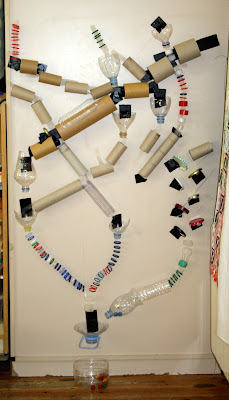
\includegraphics{media/tubes.jpg}
\caption{Think of your data `flowing' down the screen.}
\end{figure}

The `pipe' operator, \texttt{\%\textgreater{}\%} makes our data `flow' in this way:

\begin{Shaded}
\begin{Highlighting}[]
\NormalTok{big.bucket.of.data <-}\StringTok{ }\NormalTok{mtcars}

\NormalTok{big.bucket.of.data }\OperatorTok
\StringTok{  }\KeywordTok{filter}\NormalTok{(mpg }\OperatorTok{<}\DecValTok{15}\NormalTok{) }\OperatorTok
\StringTok{  }\KeywordTok{select}\NormalTok{(wt) }\OperatorTok
\StringTok{  }\NormalTok{summary}
\NormalTok{       wt       }
\NormalTok{ Min.   }\OperatorTok{:}\FloatTok{3.570}  
\NormalTok{ 1st Qu.}\OperatorTok{:}\FloatTok{3.840}  
\NormalTok{ Median }\OperatorTok{:}\FloatTok{5.250}  
\NormalTok{ Mean   }\OperatorTok{:}\FloatTok{4.686}  
\NormalTok{ 3rd Qu.}\OperatorTok{:}\FloatTok{5.345}  
\NormalTok{ Max.   }\OperatorTok{:}\FloatTok{5.424}  
\end{Highlighting}
\end{Shaded}

The \texttt{\%\textgreater{}\%} symbol makes the data flow onto the next step. Each function which
follows the pipe takes the incoming data as it's first input.

Pipes do the same thing as nesting functions, but the code stays more readable.

It's especially nice because the order in which the functions happen is the same
as the order in which we read the code (the opposite is true for nested
functions).

We can save intermediate `buckets' for use later on:

\begin{Shaded}
\begin{Highlighting}[]
\NormalTok{smaller.bucket <-}\StringTok{ }\NormalTok{big.bucket.of.data }\OperatorTok
\StringTok{  }\KeywordTok{filter}\NormalTok{(mpg }\OperatorTok{<}\DecValTok{15}\NormalTok{) }\OperatorTok
\StringTok{  }\KeywordTok{select}\NormalTok{(wt)}
\end{Highlighting}
\end{Shaded}

This is an incredibly useful pattern for processing and working with data.

We can `pour' data through a series of filters and other operations, saving
intermediate states where necessary.

You can insert the \texttt{\%\textgreater{}\%} symbol in RStdudio by typing \texttt{cmd-shift-M}, which saves
a lot of typing.

\hypertarget{mutate}{%
\subsection*{Modifying and creating new columns}\label{mutate}}
\addcontentsline{toc}{subsection}{Modifying and creating new columns}

We often want to compute new columns from data we already have.

Imagine we had heights stored in cm, and weights stored in kg for 100
participants in a study on weight loss:

\begin{Shaded}
\begin{Highlighting}[]
\KeywordTok{set.seed}\NormalTok{(}\DecValTok{1234}\NormalTok{)}

\NormalTok{weightloss <-}\StringTok{ }\KeywordTok{tibble}\NormalTok{(}
    \DataTypeTok{height_cm =} \KeywordTok{rnorm}\NormalTok{(}\DecValTok{100}\NormalTok{, }\DecValTok{150}\NormalTok{, }\DecValTok{20}\NormalTok{),}
    \DataTypeTok{weight_kg =} \KeywordTok{rnorm}\NormalTok{(}\DecValTok{100}\NormalTok{, }\DecValTok{65}\NormalTok{, }\DecValTok{10}\NormalTok{)}
\NormalTok{)}
\end{Highlighting}
\end{Shaded}

\begin{Shaded}
\begin{Highlighting}[]
\NormalTok{weightloss }\OperatorTok\StringTok{ }\NormalTok{head}
\CommentTok{# A tibble: 6 x 2}
\NormalTok{  height_cm weight_kg}
      \OperatorTok{<}\NormalTok{dbl}\OperatorTok{>}\StringTok{     }\ErrorTok{<}\NormalTok{dbl}\OperatorTok{>}
\DecValTok{1}      \FloatTok{126.}      \FloatTok{69.1}
\DecValTok{2}      \FloatTok{156.}      \FloatTok{60.3}
\DecValTok{3}      \FloatTok{172.}      \FloatTok{65.7}
\DecValTok{4}      \FloatTok{103.}      \FloatTok{60.0}
\DecValTok{5}      \FloatTok{159.}      \FloatTok{56.7}
\DecValTok{6}      \FloatTok{160.}      \FloatTok{66.7}
\end{Highlighting}
\end{Shaded}

If we want to compute each participants' Body Mass Index, we first need to
convert their height into meters. We do this with mutate:

\begin{Shaded}
\begin{Highlighting}[]
\NormalTok{weightloss }\OperatorTok
\StringTok{  }\KeywordTok{mutate}\NormalTok{(}\DataTypeTok{height_meters =}\NormalTok{ height_cm }\OperatorTok{/}\StringTok{ }\DecValTok{100}\NormalTok{) }\OperatorTok
\StringTok{  }\NormalTok{head}
\CommentTok{# A tibble: 6 x 3}
\NormalTok{  height_cm weight_kg height_meters}
      \OperatorTok{<}\NormalTok{dbl}\OperatorTok{>}\StringTok{     }\ErrorTok{<}\NormalTok{dbl}\OperatorTok{>}\StringTok{         }\ErrorTok{<}\NormalTok{dbl}\OperatorTok{>}
\DecValTok{1}      \FloatTok{126.}      \FloatTok{69.1}          \FloatTok{1.26}
\DecValTok{2}      \FloatTok{156.}      \FloatTok{60.3}          \FloatTok{1.56}
\DecValTok{3}      \FloatTok{172.}      \FloatTok{65.7}          \FloatTok{1.72}
\DecValTok{4}      \FloatTok{103.}      \FloatTok{60.0}          \FloatTok{1.03}
\DecValTok{5}      \FloatTok{159.}      \FloatTok{56.7}          \FloatTok{1.59}
\DecValTok{6}      \FloatTok{160.}      \FloatTok{66.7}          \FloatTok{1.60}
\end{Highlighting}
\end{Shaded}

We then want to calculate BMI:

\begin{Shaded}
\begin{Highlighting}[]
\NormalTok{weightloss }\OperatorTok
\StringTok{  }\KeywordTok{mutate}\NormalTok{(}\DataTypeTok{height_meters =}\NormalTok{ height_cm }\OperatorTok{/}\StringTok{ }\DecValTok{100}\NormalTok{,}
         \DataTypeTok{bmi =}\NormalTok{ weight_kg }\OperatorTok{/}\StringTok{ }\NormalTok{height_meters }\OperatorTok{^}\StringTok{ }\DecValTok{2}\NormalTok{) }\OperatorTok
\StringTok{  }\NormalTok{head}
\CommentTok{# A tibble: 6 x 4}
\NormalTok{  height_cm weight_kg height_meters   bmi}
      \OperatorTok{<}\NormalTok{dbl}\OperatorTok{>}\StringTok{     }\ErrorTok{<}\NormalTok{dbl}\OperatorTok{>}\StringTok{         }\ErrorTok{<}\NormalTok{dbl}\OperatorTok{>}\StringTok{ }\ErrorTok{<}\NormalTok{dbl}\OperatorTok{>}
\DecValTok{1}      \FloatTok{126.}      \FloatTok{69.1}          \FloatTok{1.26}  \FloatTok{43.7}
\DecValTok{2}      \FloatTok{156.}      \FloatTok{60.3}          \FloatTok{1.56}  \FloatTok{24.9}
\DecValTok{3}      \FloatTok{172.}      \FloatTok{65.7}          \FloatTok{1.72}  \FloatTok{22.3}
\DecValTok{4}      \FloatTok{103.}      \FloatTok{60.0}          \FloatTok{1.03}  \FloatTok{56.4}
\DecValTok{5}      \FloatTok{159.}      \FloatTok{56.7}          \FloatTok{1.59}  \FloatTok{22.6}
\DecValTok{6}      \FloatTok{160.}      \FloatTok{66.7}          \FloatTok{1.60}  \FloatTok{26.0}
\end{Highlighting}
\end{Shaded}

You could skip the intermediate step of converting to meters and write:
\texttt{bmi\ =\ weight\_kg\ /\ (height\_cm/100)\ \^{}\ 2}. But it's often best to be explicit and
simplify each operation.

\hypertarget{real-data}{%
\section{`Real' data}\label{real-data}}

\emph{Note: If you already lucky enough to have nicely formatted data, ready for use
in R, then you could skip this section and revisit it later,} save for the
section on \protect\hyperlink{factors-and-numerics}{factors and other variable types}.

Most tutorials and textbooks use neatly formatted example datasets to illustrate
particular techniques. However in the real-world our data can be:

\begin{itemize}
\tightlist
\item
  In the wrong format
\item
  Spread across multiple files
\item
  Badly coded, or with errors
\item
  Incomplete, with values missing for many different reasons
\end{itemize}

This chapter will give you techniques to address each of these problems.

\hypertarget{importing-data}{%
\subsection*{Importing data}\label{importing-data}}
\addcontentsline{toc}{subsection}{Importing data}

If you have data outside of R, \emph{the simplest way to import it is to first save
it as a comma or tab-separated text file}, normally with the file extension
\texttt{.csv} or \texttt{.txt}\footnote{This is easy to achieve in Excel and most other stats packages
  using the \texttt{Save\ As...} menu item}.

Let's say we have file called \texttt{angry\_moods.csv} in the same directory as our
\texttt{.Rmd} file. We can read this data using the \texttt{read\_csv()} function from the
\texttt{readr} package\footnote{There are also standard functions built into R, such as \texttt{read.csv()} or
  \texttt{read.table()} for importing data. These are fine if you can't install the
  \texttt{readr} package for some reason, but they are quite old and the default
  behaviour is sometimes counterintuitive. I recommend using the \texttt{readr}
  equivalents: \texttt{read\_csv()} or \texttt{read\_tsv()}.}:

\begin{Shaded}
\begin{Highlighting}[]
\NormalTok{angry.moods <-}\StringTok{ }\NormalTok{readr}\OperatorTok{::}\KeywordTok{read_csv}\NormalTok{(}\StringTok{'data/angry_moods.csv'}\NormalTok{)}
\KeywordTok{head}\NormalTok{(angry.moods)}
\CommentTok{# A tibble: 6 x 7}
\NormalTok{  Gender Sports Anger.Out Anger.In Control.Out Control.In Anger.Expression}
   \OperatorTok{<}\NormalTok{dbl}\OperatorTok{>}\StringTok{  }\ErrorTok{<}\NormalTok{dbl}\OperatorTok{>}\StringTok{     }\ErrorTok{<}\NormalTok{dbl}\OperatorTok{>}\StringTok{    }\ErrorTok{<}\NormalTok{dbl}\OperatorTok{>}\StringTok{       }\ErrorTok{<}\NormalTok{dbl}\OperatorTok{>}\StringTok{      }\ErrorTok{<}\NormalTok{dbl}\OperatorTok{>}\StringTok{            }\ErrorTok{<}\NormalTok{dbl}\OperatorTok{>}
\DecValTok{1}      \DecValTok{2}      \DecValTok{1}        \DecValTok{18}       \DecValTok{13}          \DecValTok{23}         \DecValTok{20}               \DecValTok{36}
\DecValTok{2}      \DecValTok{2}      \DecValTok{1}        \DecValTok{14}       \DecValTok{17}          \DecValTok{25}         \DecValTok{24}               \DecValTok{30}
\DecValTok{3}      \DecValTok{2}      \DecValTok{1}        \DecValTok{13}       \DecValTok{14}          \DecValTok{28}         \DecValTok{28}               \DecValTok{19}
\DecValTok{4}      \DecValTok{2}      \DecValTok{1}        \DecValTok{17}       \DecValTok{24}          \DecValTok{23}         \DecValTok{23}               \DecValTok{43}
\DecValTok{5}      \DecValTok{1}      \DecValTok{1}        \DecValTok{16}       \DecValTok{17}          \DecValTok{26}         \DecValTok{28}               \DecValTok{27}
\DecValTok{6}      \DecValTok{1}      \DecValTok{1}        \DecValTok{16}       \DecValTok{22}          \DecValTok{25}         \DecValTok{23}               \DecValTok{38}
\end{Highlighting}
\end{Shaded}

As you can see, when loading the \texttt{.csv} file the \texttt{read\_csv()} makes some
assumptions about the \emph{type} of data the file contains. In this case, all the
columns contain integer values. It's worth checking this message to make sure
that stray cells in the file you are importing don't cause problems when
importing. Excel won't complain about this sort of thing, but R is more strict
and won't mix text and numbers in the same column.

A common error is for stray notes or text values in a spreadsheet to cause a
column which should be numeric to be converted to the \texttt{character} type.

Once it's loaded, you can use this new dataset like any other:

\begin{Shaded}
\begin{Highlighting}[]
\KeywordTok{pairs}\NormalTok{(angry.moods)}
\end{Highlighting}
\end{Shaded}

\includegraphics{import-export_files/figure-latex/unnamed-chunk-4-1.pdf}

\hypertarget{importing-data-from-the-web}{%
\subsubsection*{Importing data over the web}\label{importing-data-from-the-web}}
\addcontentsline{toc}{subsubsection}{Importing data over the web}

One neat feature of the \texttt{readr} package is that you can import data from the
web, using a URL rather than a filename on your local computer. This can be
really helpful when sharing data and code with colleagues. For example, we can
load the \texttt{angry\_moods.csv} file from a URL:

\begin{Shaded}
\begin{Highlighting}[]
\NormalTok{angry.moods.from.url <-}\StringTok{ }\NormalTok{readr}\OperatorTok{::}\KeywordTok{read_csv}\NormalTok{(}
  \StringTok{"https://raw.githubusercontent.com/benwhalley/just-enough-r/master/angry_moods.csv"}\NormalTok{)}

\KeywordTok{head}\NormalTok{(angry.moods.from.url)}
\end{Highlighting}
\end{Shaded}

\hypertarget{importing-proprietary-formats}{%
\subsubsection*{Importing from SPSS and other packages}\label{importing-proprietary-formats}}
\addcontentsline{toc}{subsubsection}{Importing from SPSS and other packages}

This is often more trouble than it's worth. If using Excel for example, it's
best just to save your data a csv file first and import that.

But if you really must use other formats see
\url{https://www.datacamp.com/community/tutorials/r-data-import-tutorial}.

\hypertarget{saving-and-exporting}{%
\subsection*{Saving and exporting}\label{saving-and-exporting}}
\addcontentsline{toc}{subsection}{Saving and exporting}

Before you start saving data in csv or any other format, as yourself: ``Do I need
to save \emph{this} dataset, or should I simply save my raw data and code?''

Oftentimes it's best to keep only your raw datafiles, with the R code you used
to process them. This keeps your disk tidier, and avoids confusion with multiple
versions of files.

If it takes a long time to process your data though you might want to save
interim steps. And if you share your data (which you should) you might also want
to save simplified or anonymised versions of it, in widely-accessible formats.

\hypertarget{use-csv}{%
\subsubsection*{Use CSV files}\label{use-csv}}
\addcontentsline{toc}{subsubsection}{Use CSV files}

Comma-separated-values files are a plain text format which are idea for storing
and sharing your data. They are:

\begin{itemize}
\tightlist
\item
  Understood by almost every piece of software, ever
\item
  Will be readable in future
\item
  Perfect for storing 2D data (like dataframes)
\item
  Readable by humans (just open them in Notepad)
\end{itemize}

Commercial formats like Excel, SPSS (.sav) and Stata (.dta) don't have these
properties.

Although CSV has some disadvantages, they are all easily overcome if you
\protect\hyperlink{save-intermediate-steps}{save the steps of your data processing and analysis in your R code},
see below.

Saving a dataframe to .csv is as simple as:

\begin{Shaded}
\begin{Highlighting}[]
\NormalTok{readr}\OperatorTok{::}\KeywordTok{write_csv}\NormalTok{(mtcars, }\StringTok{'mtcars.csv'}\NormalTok{)}
\end{Highlighting}
\end{Shaded}

If you run this within an RMarkdown document, this will create the new csv file
in the same directory as your \texttt{.Rmd} file.

{You can also use the \texttt{write.csv()} function in base R, but this version from
\texttt{readr} is faster and has more sensible defalts (e.g.~it doesn't write rownames,
but does save column names in the first row)}

\hypertarget{save-intermediate-steps}{%
\paragraph{Save processes, not just outcomes}\label{save-intermediate-steps}}
\addcontentsline{toc}{paragraph}{Save processes, not just outcomes}

Many students (and academics) make errors in their analyses because they process
data by hand (e.g.~editing files in Excel) or use GUI tools to run analyses.

In both cases these errors are hard to identify or rectify because only the
outputs of the analysis can be saved, and \emph{no record has been made of how these
outputs were produced}.

In contrast, if you do your data processing and analysis in R/RMarkdown you
benefit from a concrete, repeatable series of steps which can be
checked/verified by others. This can also save lots of time if you need to
processing additional data later on (e.g.~if you run more participants).

Some principles to follow when working:

\begin{itemize}
\item
  Save your raw data in the simplest possible format, in CSV
\item
  Always include column names in the file
\item
  Use descriptive names, but with a regular strucuture.
\item
  Never include spaces or special characters in the column names. Use
  underscores (\texttt{\_}) if you want to make things more readable.
\item
  Make names \textless{}20 characters in length if possible
\end{itemize}

\hypertarget{saving-interim-steps}{%
\paragraph{Saving interim steps}\label{saving-interim-steps}}
\addcontentsline{toc}{paragraph}{Saving interim steps}

If you are saving data to use again later in R, the best format is RDS. Saving
files to RDS \protect\hyperlink{rds-files}{is covered in a later section (click to see)}.

If you are saving interim steps but think you might possibly want to access it
from other programmes in future use csv though.

To save something using RDS:

\begin{Shaded}
\begin{Highlighting}[]
\CommentTok{# create a huge df of random numbers...}
\NormalTok{massive.df <-}\StringTok{ }\KeywordTok{data_frame}\NormalTok{(}\DataTypeTok{nums =} \KeywordTok{rnorm}\NormalTok{(}\DecValTok{1}\OperatorTok{:}\FloatTok{1e6}\NormalTok{))}
\KeywordTok{saveRDS}\NormalTok{(massive.df, }\DataTypeTok{file=}\StringTok{"massive.RDS"}\NormalTok{)}
\end{Highlighting}
\end{Shaded}

Then later on you can load it like this:

\begin{Shaded}
\begin{Highlighting}[]
\NormalTok{restored.massive.df <-}\StringTok{  }\KeywordTok{readRDS}\NormalTok{(}\StringTok{'massive.RDS'}\NormalTok{)}
\end{Highlighting}
\end{Shaded}

{If you do this in RMarkdown, by default the RDS files will be saved in the same
directory as your .Rmd file.}

\hypertarget{archiving-publication-and-sharing}{%
\subsubsection*{Archiving, publication and sharing}\label{archiving-publication-and-sharing}}
\addcontentsline{toc}{subsubsection}{Archiving, publication and sharing}

If you want to share data with someone else, or open it in a different software
package, using `.csv' format is strongly recommended unless some other format is
common in your field.

When archiving data, or sharing with others, you must document what each column
measures, and any processing steps used to create the file. RMarkdown is a good
way of doing this because it can combine the processing with narrative
explaining what is being done, and why.

\hypertarget{multiple-raw-data-files}{%
\subsection*{Dealing with multiple files}\label{multiple-raw-data-files}}
\addcontentsline{toc}{subsection}{Dealing with multiple files}

Often you will have multiple data files files - for example, those produced by
\href{http://www.psychopy.org}{experimental software}.

This is one of the few times when you might have to do something resembling
`real programming', but it's still fairly straightforward.

In the \protect\hyperlink{trad-rm-anova}{repeated measures Anova example later on in this guide}
we encounter some data from an experiment where reaction times were recorded in
25 trials (\texttt{Trial}) before and after (\texttt{Time}) one of 4 experimental
manipulations (\texttt{Condition\ =\ \{1,2,3,4\}}). There were 48 participants in total:

Let's say that we have saved all the files are in a single directory, and these
are numbered sequentially: \texttt{person01.csv}, \texttt{person02.csv} and so on.

Using the \texttt{list.files()} function we can list the contents of a directory on the
hard drive:

\begin{Shaded}
\begin{Highlighting}[]
\KeywordTok{list.files}\NormalTok{(}\StringTok{'data/multiple-file-example/'}\NormalTok{)}
\NormalTok{ [}\DecValTok{1}\NormalTok{] }\StringTok{"person1.csv"}  \StringTok{"person10.csv"} \StringTok{"person11.csv"} \StringTok{"person12.csv"}
\NormalTok{ [}\DecValTok{5}\NormalTok{] }\StringTok{"person13.csv"} \StringTok{"person14.csv"} \StringTok{"person15.csv"} \StringTok{"person16.csv"}
\NormalTok{ [}\DecValTok{9}\NormalTok{] }\StringTok{"person17.csv"} \StringTok{"person18.csv"} \StringTok{"person19.csv"} \StringTok{"person2.csv"} 
\NormalTok{[}\DecValTok{13}\NormalTok{] }\StringTok{"person20.csv"} \StringTok{"person21.csv"} \StringTok{"person22.csv"} \StringTok{"person23.csv"}
\NormalTok{[}\DecValTok{17}\NormalTok{] }\StringTok{"person24.csv"} \StringTok{"person25.csv"} \StringTok{"person26.csv"} \StringTok{"person27.csv"}
\NormalTok{[}\DecValTok{21}\NormalTok{] }\StringTok{"person28.csv"} \StringTok{"person29.csv"} \StringTok{"person3.csv"}  \StringTok{"person30.csv"}
\NormalTok{[}\DecValTok{25}\NormalTok{] }\StringTok{"person31.csv"} \StringTok{"person32.csv"} \StringTok{"person33.csv"} \StringTok{"person34.csv"}
\NormalTok{[}\DecValTok{29}\NormalTok{] }\StringTok{"person35.csv"} \StringTok{"person36.csv"} \StringTok{"person37.csv"} \StringTok{"person38.csv"}
\NormalTok{[}\DecValTok{33}\NormalTok{] }\StringTok{"person39.csv"} \StringTok{"person4.csv"}  \StringTok{"person40.csv"} \StringTok{"person41.csv"}
\NormalTok{[}\DecValTok{37}\NormalTok{] }\StringTok{"person42.csv"} \StringTok{"person43.csv"} \StringTok{"person44.csv"} \StringTok{"person45.csv"}
\NormalTok{[}\DecValTok{41}\NormalTok{] }\StringTok{"person46.csv"} \StringTok{"person47.csv"} \StringTok{"person48.csv"} \StringTok{"person5.csv"} 
\NormalTok{[}\DecValTok{45}\NormalTok{] }\StringTok{"person6.csv"}  \StringTok{"person7.csv"}  \StringTok{"person8.csv"}  \StringTok{"person9.csv"} 
\end{Highlighting}
\end{Shaded}

The \texttt{list.files()} function creates a \protect\hyperlink{vectors}{vector} of the names of all the
files in the directory.

At this point, there are many, many ways of importing the contents of these
files, but below we use a technique which is concise, reliable, and less
error-prone than many others. It also continues to use the \texttt{dplyr} library.

This approach has 3 steps:

\begin{enumerate}
\def\labelenumi{\arabic{enumi}.}
\tightlist
\item
  Put all the names of the .csv files into a dataframe.
\item
  For each row in the dataframe, run a function which imports the file as a
  dataframe.
\item
  Combine all these dataframes together.
\end{enumerate}

Putting the filenames into a dataframe

Because \texttt{list.files} produces a vector, we can make them a column in a new
dataframe:

\begin{Shaded}
\begin{Highlighting}[]
\NormalTok{raw.files <-}\StringTok{ }\KeywordTok{data_frame}\NormalTok{(}\DataTypeTok{filename =} \KeywordTok{list.files}\NormalTok{(}\StringTok{'data/multiple-file-example/'}\NormalTok{))}
\end{Highlighting}
\end{Shaded}

And we can make a new column with the complete path (i.e.~including the
directory holding the files), using the \protect\hyperlink{paste}{\texttt{paste0}} which combines
strings of text. We wouldn't have to do this if the raw files were in the same
directory as our RMarkdown file, but that would get messy.

\begin{Shaded}
\begin{Highlighting}[]
\NormalTok{raw.file.paths <-}\StringTok{ }\NormalTok{raw.files  }\OperatorTok
\StringTok{  }\KeywordTok{mutate}\NormalTok{(}\DataTypeTok{filepath =} \KeywordTok{paste0}\NormalTok{(}\StringTok{"data/multiple-file-example/"}\NormalTok{, filename))}

\NormalTok{raw.file.paths }\OperatorTok
\StringTok{  }\KeywordTok{head}\NormalTok{(}\DecValTok{3}\NormalTok{)}
\CommentTok{# A tibble: 3 x 2}
\NormalTok{  filename     filepath                               }
  \OperatorTok{<}\NormalTok{chr}\OperatorTok{>}\StringTok{        }\ErrorTok{<}\NormalTok{chr}\OperatorTok{>}\StringTok{                                  }
\DecValTok{1}\NormalTok{ person1.csv  data}\OperatorTok{/}\NormalTok{multiple}\OperatorTok{-}\NormalTok{file}\OperatorTok{-}\NormalTok{example}\OperatorTok{/}\NormalTok{person1.csv }
\DecValTok{2}\NormalTok{ person10.csv data}\OperatorTok{/}\NormalTok{multiple}\OperatorTok{-}\NormalTok{file}\OperatorTok{-}\NormalTok{example}\OperatorTok{/}\NormalTok{person10.csv}
\DecValTok{3}\NormalTok{ person11.csv data}\OperatorTok{/}\NormalTok{multiple}\OperatorTok{-}\NormalTok{file}\OperatorTok{-}\NormalTok{example}\OperatorTok{/}\NormalTok{person11.csv}
\end{Highlighting}
\end{Shaded}

Using \texttt{do()}

We can then use the \texttt{do()} function in \texttt{dplyr::} to import the data for each
file and combine the results in a single dataframe.

The \texttt{do()} function allows us to run any R function for each group or row in a
dataframe.

The means that our original dataframe is broken up into chunks (either groups of
rows, if we use \texttt{group\_by()}, or individual rows if we use \texttt{rowwise()}) and each
chunk is fed to the function we specify. This function must do it's work and
return a new dataframe, and these are then combined into a single larger
dataframe.

So in this example, we break our dataframe of filenames up into individual rows
using \texttt{rowwise} and then specify the \texttt{read\_csv} function which takes the name of
a csv file, and returns the content as a dataframe
(\protect\hyperlink{importing-data}{see the importing data section}).

For example:

\begin{Shaded}
\begin{Highlighting}[]
\NormalTok{raw.data <-}\StringTok{ }\NormalTok{raw.file.paths }\OperatorTok
\StringTok{  }\CommentTok{# 'do' the function for each row in turn}
\StringTok{  }\KeywordTok{rowwise}\NormalTok{() }\OperatorTok
\StringTok{  }\KeywordTok{do}\NormalTok{(., }\KeywordTok{read_csv}\NormalTok{(}\DataTypeTok{file=}\NormalTok{.}\OperatorTok{$}\NormalTok{filepath))}
\end{Highlighting}
\end{Shaded}

We can check these data look OK by sampling 10 rows at random:

\begin{Shaded}
\begin{Highlighting}[]
\NormalTok{raw.data }\OperatorTok
\StringTok{  }\KeywordTok{sample_n}\NormalTok{(}\DecValTok{10}\NormalTok{) }\OperatorTok
\StringTok{  }\KeywordTok{pander}\NormalTok{()}
\end{Highlighting}
\end{Shaded}

\begin{longtable}[]{@{}ccccc@{}}
\toprule
\begin{minipage}[b]{0.14\columnwidth}\centering
Condition\strut
\end{minipage} & \begin{minipage}[b]{0.10\columnwidth}\centering
trial\strut
\end{minipage} & \begin{minipage}[b]{0.08\columnwidth}\centering
time\strut
\end{minipage} & \begin{minipage}[b]{0.11\columnwidth}\centering
person\strut
\end{minipage} & \begin{minipage}[b]{0.11\columnwidth}\centering
RT\strut
\end{minipage}\tabularnewline
\midrule
\endhead
\begin{minipage}[t]{0.14\columnwidth}\centering
3\strut
\end{minipage} & \begin{minipage}[t]{0.10\columnwidth}\centering
17\strut
\end{minipage} & \begin{minipage}[t]{0.08\columnwidth}\centering
2\strut
\end{minipage} & \begin{minipage}[t]{0.11\columnwidth}\centering
35\strut
\end{minipage} & \begin{minipage}[t]{0.11\columnwidth}\centering
360.2\strut
\end{minipage}\tabularnewline
\begin{minipage}[t]{0.14\columnwidth}\centering
1\strut
\end{minipage} & \begin{minipage}[t]{0.10\columnwidth}\centering
3\strut
\end{minipage} & \begin{minipage}[t]{0.08\columnwidth}\centering
2\strut
\end{minipage} & \begin{minipage}[t]{0.11\columnwidth}\centering
1\strut
\end{minipage} & \begin{minipage}[t]{0.11\columnwidth}\centering
220.4\strut
\end{minipage}\tabularnewline
\begin{minipage}[t]{0.14\columnwidth}\centering
1\strut
\end{minipage} & \begin{minipage}[t]{0.10\columnwidth}\centering
15\strut
\end{minipage} & \begin{minipage}[t]{0.08\columnwidth}\centering
2\strut
\end{minipage} & \begin{minipage}[t]{0.11\columnwidth}\centering
7\strut
\end{minipage} & \begin{minipage}[t]{0.11\columnwidth}\centering
191\strut
\end{minipage}\tabularnewline
\begin{minipage}[t]{0.14\columnwidth}\centering
4\strut
\end{minipage} & \begin{minipage}[t]{0.10\columnwidth}\centering
1\strut
\end{minipage} & \begin{minipage}[t]{0.08\columnwidth}\centering
2\strut
\end{minipage} & \begin{minipage}[t]{0.11\columnwidth}\centering
37\strut
\end{minipage} & \begin{minipage}[t]{0.11\columnwidth}\centering
361\strut
\end{minipage}\tabularnewline
\begin{minipage}[t]{0.14\columnwidth}\centering
3\strut
\end{minipage} & \begin{minipage}[t]{0.10\columnwidth}\centering
19\strut
\end{minipage} & \begin{minipage}[t]{0.08\columnwidth}\centering
1\strut
\end{minipage} & \begin{minipage}[t]{0.11\columnwidth}\centering
28\strut
\end{minipage} & \begin{minipage}[t]{0.11\columnwidth}\centering
246.8\strut
\end{minipage}\tabularnewline
\begin{minipage}[t]{0.14\columnwidth}\centering
3\strut
\end{minipage} & \begin{minipage}[t]{0.10\columnwidth}\centering
16\strut
\end{minipage} & \begin{minipage}[t]{0.08\columnwidth}\centering
1\strut
\end{minipage} & \begin{minipage}[t]{0.11\columnwidth}\centering
30\strut
\end{minipage} & \begin{minipage}[t]{0.11\columnwidth}\centering
199.6\strut
\end{minipage}\tabularnewline
\begin{minipage}[t]{0.14\columnwidth}\centering
3\strut
\end{minipage} & \begin{minipage}[t]{0.10\columnwidth}\centering
15\strut
\end{minipage} & \begin{minipage}[t]{0.08\columnwidth}\centering
2\strut
\end{minipage} & \begin{minipage}[t]{0.11\columnwidth}\centering
30\strut
\end{minipage} & \begin{minipage}[t]{0.11\columnwidth}\centering
206.2\strut
\end{minipage}\tabularnewline
\begin{minipage}[t]{0.14\columnwidth}\centering
4\strut
\end{minipage} & \begin{minipage}[t]{0.10\columnwidth}\centering
5\strut
\end{minipage} & \begin{minipage}[t]{0.08\columnwidth}\centering
1\strut
\end{minipage} & \begin{minipage}[t]{0.11\columnwidth}\centering
39\strut
\end{minipage} & \begin{minipage}[t]{0.11\columnwidth}\centering
295.5\strut
\end{minipage}\tabularnewline
\begin{minipage}[t]{0.14\columnwidth}\centering
2\strut
\end{minipage} & \begin{minipage}[t]{0.10\columnwidth}\centering
22\strut
\end{minipage} & \begin{minipage}[t]{0.08\columnwidth}\centering
2\strut
\end{minipage} & \begin{minipage}[t]{0.11\columnwidth}\centering
15\strut
\end{minipage} & \begin{minipage}[t]{0.11\columnwidth}\centering
298.7\strut
\end{minipage}\tabularnewline
\begin{minipage}[t]{0.14\columnwidth}\centering
1\strut
\end{minipage} & \begin{minipage}[t]{0.10\columnwidth}\centering
24\strut
\end{minipage} & \begin{minipage}[t]{0.08\columnwidth}\centering
1\strut
\end{minipage} & \begin{minipage}[t]{0.11\columnwidth}\centering
5\strut
\end{minipage} & \begin{minipage}[t]{0.11\columnwidth}\centering
237.2\strut
\end{minipage}\tabularnewline
\bottomrule
\end{longtable}

\hypertarget{using-custom-functions-with-do}{%
\subparagraph{\texorpdfstring{Using custom functions with \texttt{do()}}{Using custom functions with do()}}\label{using-custom-functions-with-do}}
\addcontentsline{toc}{subparagraph}{Using custom functions with \texttt{do()}}

In this example, each of the raw data files included the participant number (the
\texttt{person} variable). However, this isn't always the case.

This isn't a problem though, if we create our own
\protect\hyperlink{helper-functions}{helper function} to import the data. Writing small functions
in R is very easy, and the example below wraps the \texttt{read.csv()} function and
adds a new colum, \texttt{filename} to the imported data frame which would enable us to
keep track of where each row in the final combined dataset came from.

This is the helper function:

\begin{Shaded}
\begin{Highlighting}[]
\NormalTok{read.csv.and.add.filename <-}\StringTok{ }\ControlFlowTok{function}\NormalTok{(filepath)\{}
  \KeywordTok{read_csv}\NormalTok{(filepath) }\OperatorTok
\StringTok{    }\KeywordTok{mutate}\NormalTok{(}\DataTypeTok{filepath=}\NormalTok{filepath)}
\NormalTok{\}}
\end{Highlighting}
\end{Shaded}

In English, you should read this as:

\begin{quote}
``Create a new R function called \texttt{read.csv.and.add.filename} which expects to
be passed a path to a csv file as an input. This function reads the csv file
at the path (converting it to a dataframe), and adds a new column containing
the original file path it read from. It then returns this dataframe.''
\end{quote}

We can use our helper function with \texttt{do()} in place of the bare \texttt{read\_csv}
function we used before:

\begin{Shaded}
\begin{Highlighting}[]
\NormalTok{raw.data.with.paths <-}\StringTok{ }\NormalTok{raw.file.paths }\OperatorTok
\StringTok{  }\KeywordTok{rowwise}\NormalTok{() }\OperatorTok
\StringTok{  }\KeywordTok{do}\NormalTok{(., }\KeywordTok{read.csv.and.add.filename}\NormalTok{(.}\OperatorTok{$}\NormalTok{filepath))}

\NormalTok{raw.data.with.paths }\OperatorTok
\StringTok{  }\KeywordTok{sample_n}\NormalTok{(}\DecValTok{10}\NormalTok{) }\OperatorTok
\StringTok{  }\KeywordTok{pander}\NormalTok{()}
\end{Highlighting}
\end{Shaded}

\begin{longtable}[]{@{}ccccc@{}}
\caption{Table continues below}\tabularnewline
\toprule
\begin{minipage}[b]{0.14\columnwidth}\centering
Condition\strut
\end{minipage} & \begin{minipage}[b]{0.10\columnwidth}\centering
trial\strut
\end{minipage} & \begin{minipage}[b]{0.08\columnwidth}\centering
time\strut
\end{minipage} & \begin{minipage}[b]{0.11\columnwidth}\centering
person\strut
\end{minipage} & \begin{minipage}[b]{0.11\columnwidth}\centering
RT\strut
\end{minipage}\tabularnewline
\midrule
\endfirsthead
\toprule
\begin{minipage}[b]{0.14\columnwidth}\centering
Condition\strut
\end{minipage} & \begin{minipage}[b]{0.10\columnwidth}\centering
trial\strut
\end{minipage} & \begin{minipage}[b]{0.08\columnwidth}\centering
time\strut
\end{minipage} & \begin{minipage}[b]{0.11\columnwidth}\centering
person\strut
\end{minipage} & \begin{minipage}[b]{0.11\columnwidth}\centering
RT\strut
\end{minipage}\tabularnewline
\midrule
\endhead
\begin{minipage}[t]{0.14\columnwidth}\centering
2\strut
\end{minipage} & \begin{minipage}[t]{0.10\columnwidth}\centering
25\strut
\end{minipage} & \begin{minipage}[t]{0.08\columnwidth}\centering
2\strut
\end{minipage} & \begin{minipage}[t]{0.11\columnwidth}\centering
17\strut
\end{minipage} & \begin{minipage}[t]{0.11\columnwidth}\centering
90.31\strut
\end{minipage}\tabularnewline
\begin{minipage}[t]{0.14\columnwidth}\centering
2\strut
\end{minipage} & \begin{minipage}[t]{0.10\columnwidth}\centering
5\strut
\end{minipage} & \begin{minipage}[t]{0.08\columnwidth}\centering
1\strut
\end{minipage} & \begin{minipage}[t]{0.11\columnwidth}\centering
22\strut
\end{minipage} & \begin{minipage}[t]{0.11\columnwidth}\centering
341.3\strut
\end{minipage}\tabularnewline
\begin{minipage}[t]{0.14\columnwidth}\centering
1\strut
\end{minipage} & \begin{minipage}[t]{0.10\columnwidth}\centering
2\strut
\end{minipage} & \begin{minipage}[t]{0.08\columnwidth}\centering
1\strut
\end{minipage} & \begin{minipage}[t]{0.11\columnwidth}\centering
8\strut
\end{minipage} & \begin{minipage}[t]{0.11\columnwidth}\centering
239.3\strut
\end{minipage}\tabularnewline
\begin{minipage}[t]{0.14\columnwidth}\centering
4\strut
\end{minipage} & \begin{minipage}[t]{0.10\columnwidth}\centering
13\strut
\end{minipage} & \begin{minipage}[t]{0.08\columnwidth}\centering
1\strut
\end{minipage} & \begin{minipage}[t]{0.11\columnwidth}\centering
42\strut
\end{minipage} & \begin{minipage}[t]{0.11\columnwidth}\centering
197.1\strut
\end{minipage}\tabularnewline
\begin{minipage}[t]{0.14\columnwidth}\centering
2\strut
\end{minipage} & \begin{minipage}[t]{0.10\columnwidth}\centering
17\strut
\end{minipage} & \begin{minipage}[t]{0.08\columnwidth}\centering
1\strut
\end{minipage} & \begin{minipage}[t]{0.11\columnwidth}\centering
16\strut
\end{minipage} & \begin{minipage}[t]{0.11\columnwidth}\centering
169.5\strut
\end{minipage}\tabularnewline
\begin{minipage}[t]{0.14\columnwidth}\centering
2\strut
\end{minipage} & \begin{minipage}[t]{0.10\columnwidth}\centering
6\strut
\end{minipage} & \begin{minipage}[t]{0.08\columnwidth}\centering
2\strut
\end{minipage} & \begin{minipage}[t]{0.11\columnwidth}\centering
15\strut
\end{minipage} & \begin{minipage}[t]{0.11\columnwidth}\centering
166.4\strut
\end{minipage}\tabularnewline
\begin{minipage}[t]{0.14\columnwidth}\centering
3\strut
\end{minipage} & \begin{minipage}[t]{0.10\columnwidth}\centering
22\strut
\end{minipage} & \begin{minipage}[t]{0.08\columnwidth}\centering
1\strut
\end{minipage} & \begin{minipage}[t]{0.11\columnwidth}\centering
30\strut
\end{minipage} & \begin{minipage}[t]{0.11\columnwidth}\centering
214\strut
\end{minipage}\tabularnewline
\begin{minipage}[t]{0.14\columnwidth}\centering
4\strut
\end{minipage} & \begin{minipage}[t]{0.10\columnwidth}\centering
3\strut
\end{minipage} & \begin{minipage}[t]{0.08\columnwidth}\centering
1\strut
\end{minipage} & \begin{minipage}[t]{0.11\columnwidth}\centering
48\strut
\end{minipage} & \begin{minipage}[t]{0.11\columnwidth}\centering
238.7\strut
\end{minipage}\tabularnewline
\begin{minipage}[t]{0.14\columnwidth}\centering
4\strut
\end{minipage} & \begin{minipage}[t]{0.10\columnwidth}\centering
6\strut
\end{minipage} & \begin{minipage}[t]{0.08\columnwidth}\centering
2\strut
\end{minipage} & \begin{minipage}[t]{0.11\columnwidth}\centering
48\strut
\end{minipage} & \begin{minipage}[t]{0.11\columnwidth}\centering
273.5\strut
\end{minipage}\tabularnewline
\begin{minipage}[t]{0.14\columnwidth}\centering
2\strut
\end{minipage} & \begin{minipage}[t]{0.10\columnwidth}\centering
6\strut
\end{minipage} & \begin{minipage}[t]{0.08\columnwidth}\centering
1\strut
\end{minipage} & \begin{minipage}[t]{0.11\columnwidth}\centering
15\strut
\end{minipage} & \begin{minipage}[t]{0.11\columnwidth}\centering
232.1\strut
\end{minipage}\tabularnewline
\bottomrule
\end{longtable}

\begin{longtable}[]{@{}c@{}}
\toprule
\begin{minipage}[b]{0.57\columnwidth}\centering
filepath\strut
\end{minipage}\tabularnewline
\midrule
\endhead
\begin{minipage}[t]{0.57\columnwidth}\centering
data/multiple-file-example/person17.csv\strut
\end{minipage}\tabularnewline
\begin{minipage}[t]{0.57\columnwidth}\centering
data/multiple-file-example/person22.csv\strut
\end{minipage}\tabularnewline
\begin{minipage}[t]{0.57\columnwidth}\centering
data/multiple-file-example/person8.csv\strut
\end{minipage}\tabularnewline
\begin{minipage}[t]{0.57\columnwidth}\centering
data/multiple-file-example/person42.csv\strut
\end{minipage}\tabularnewline
\begin{minipage}[t]{0.57\columnwidth}\centering
data/multiple-file-example/person16.csv\strut
\end{minipage}\tabularnewline
\begin{minipage}[t]{0.57\columnwidth}\centering
data/multiple-file-example/person15.csv\strut
\end{minipage}\tabularnewline
\begin{minipage}[t]{0.57\columnwidth}\centering
data/multiple-file-example/person30.csv\strut
\end{minipage}\tabularnewline
\begin{minipage}[t]{0.57\columnwidth}\centering
data/multiple-file-example/person48.csv\strut
\end{minipage}\tabularnewline
\begin{minipage}[t]{0.57\columnwidth}\centering
data/multiple-file-example/person48.csv\strut
\end{minipage}\tabularnewline
\begin{minipage}[t]{0.57\columnwidth}\centering
data/multiple-file-example/person15.csv\strut
\end{minipage}\tabularnewline
\bottomrule
\end{longtable}

At this point you might need to
\protect\hyperlink{extract-to-split-column-names}{use the \texttt{extract()} or \texttt{separate()} functions}
to post-process the filename and re-create the \texttt{person} variable from this
(although in this case that's already been done for us).

\hypertarget{joining-data}{%
\subsection*{Joining different datasets}\label{joining-data}}
\addcontentsline{toc}{subsection}{Joining different datasets}

Many analyses combine data from different sources.

Even within a single study, you may find that you have different datafiles (
e.g.~spreadsheets) for different sorts of information. For example you might have

\begin{enumerate}
\def\labelenumi{\arabic{enumi}.}
\item
  Multiple csv files output by experimental software.
\item
  A spreadsheet of demographic characteristics of participants (e.g.~their age,
  gender, handedness)
\item
  Questionnaire data, collected before the reaction time task.
\end{enumerate}

Your main analysis might want to model individual RTs using predictors including
age, handedness or some personality variable. Thus, you probably want data which
look something like this:

\begin{Shaded}
\begin{Highlighting}[]
\NormalTok{df }\OperatorTok
\StringTok{  }\KeywordTok{pander}\NormalTok{()}
\end{Highlighting}
\end{Shaded}

\begin{longtable}[]{@{}cccccccc@{}}
\toprule
\begin{minipage}[b]{0.09\columnwidth}\centering
person\strut
\end{minipage} & \begin{minipage}[b]{0.08\columnwidth}\centering
trial\strut
\end{minipage} & \begin{minipage}[b]{0.12\columnwidth}\centering
condition\strut
\end{minipage} & \begin{minipage}[b]{0.09\columnwidth}\centering
female\strut
\end{minipage} & \begin{minipage}[b]{0.14\columnwidth}\centering
left.handed\strut
\end{minipage} & \begin{minipage}[b]{0.06\columnwidth}\centering
age\strut
\end{minipage} & \begin{minipage}[b]{0.15\columnwidth}\centering
extraversion\strut
\end{minipage} & \begin{minipage}[b]{0.08\columnwidth}\centering
RT\strut
\end{minipage}\tabularnewline
\midrule
\endhead
\begin{minipage}[t]{0.09\columnwidth}\centering
1\strut
\end{minipage} & \begin{minipage}[t]{0.08\columnwidth}\centering
1\strut
\end{minipage} & \begin{minipage}[t]{0.12\columnwidth}\centering
A\strut
\end{minipage} & \begin{minipage}[t]{0.09\columnwidth}\centering
TRUE\strut
\end{minipage} & \begin{minipage}[t]{0.14\columnwidth}\centering
FALSE\strut
\end{minipage} & \begin{minipage}[t]{0.06\columnwidth}\centering
19\strut
\end{minipage} & \begin{minipage}[t]{0.15\columnwidth}\centering
50\strut
\end{minipage} & \begin{minipage}[t]{0.08\columnwidth}\centering
251.7\strut
\end{minipage}\tabularnewline
\begin{minipage}[t]{0.09\columnwidth}\centering
1\strut
\end{minipage} & \begin{minipage}[t]{0.08\columnwidth}\centering
2\strut
\end{minipage} & \begin{minipage}[t]{0.12\columnwidth}\centering
A\strut
\end{minipage} & \begin{minipage}[t]{0.09\columnwidth}\centering
TRUE\strut
\end{minipage} & \begin{minipage}[t]{0.14\columnwidth}\centering
FALSE\strut
\end{minipage} & \begin{minipage}[t]{0.06\columnwidth}\centering
19\strut
\end{minipage} & \begin{minipage}[t]{0.15\columnwidth}\centering
50\strut
\end{minipage} & \begin{minipage}[t]{0.08\columnwidth}\centering
311.1\strut
\end{minipage}\tabularnewline
\begin{minipage}[t]{0.09\columnwidth}\centering
1\strut
\end{minipage} & \begin{minipage}[t]{0.08\columnwidth}\centering
3\strut
\end{minipage} & \begin{minipage}[t]{0.12\columnwidth}\centering
A\strut
\end{minipage} & \begin{minipage}[t]{0.09\columnwidth}\centering
TRUE\strut
\end{minipage} & \begin{minipage}[t]{0.14\columnwidth}\centering
FALSE\strut
\end{minipage} & \begin{minipage}[t]{0.06\columnwidth}\centering
19\strut
\end{minipage} & \begin{minipage}[t]{0.15\columnwidth}\centering
50\strut
\end{minipage} & \begin{minipage}[t]{0.08\columnwidth}\centering
343.4\strut
\end{minipage}\tabularnewline
\begin{minipage}[t]{0.09\columnwidth}\centering
1\strut
\end{minipage} & \begin{minipage}[t]{0.08\columnwidth}\centering
\ldots{}\strut
\end{minipage} & \begin{minipage}[t]{0.12\columnwidth}\centering
A\strut
\end{minipage} & \begin{minipage}[t]{0.09\columnwidth}\centering
TRUE\strut
\end{minipage} & \begin{minipage}[t]{0.14\columnwidth}\centering
FALSE\strut
\end{minipage} & \begin{minipage}[t]{0.06\columnwidth}\centering
19\strut
\end{minipage} & \begin{minipage}[t]{0.15\columnwidth}\centering
50\strut
\end{minipage} & \begin{minipage}[t]{0.08\columnwidth}\centering
206.2\strut
\end{minipage}\tabularnewline
\begin{minipage}[t]{0.09\columnwidth}\centering
2\strut
\end{minipage} & \begin{minipage}[t]{0.08\columnwidth}\centering
1\strut
\end{minipage} & \begin{minipage}[t]{0.12\columnwidth}\centering
B\strut
\end{minipage} & \begin{minipage}[t]{0.09\columnwidth}\centering
FALSE\strut
\end{minipage} & \begin{minipage}[t]{0.14\columnwidth}\centering
FALSE\strut
\end{minipage} & \begin{minipage}[t]{0.06\columnwidth}\centering
24\strut
\end{minipage} & \begin{minipage}[t]{0.15\columnwidth}\centering
34\strut
\end{minipage} & \begin{minipage}[t]{0.08\columnwidth}\centering
317.2\strut
\end{minipage}\tabularnewline
\begin{minipage}[t]{0.09\columnwidth}\centering
2\strut
\end{minipage} & \begin{minipage}[t]{0.08\columnwidth}\centering
2\strut
\end{minipage} & \begin{minipage}[t]{0.12\columnwidth}\centering
B\strut
\end{minipage} & \begin{minipage}[t]{0.09\columnwidth}\centering
FALSE\strut
\end{minipage} & \begin{minipage}[t]{0.14\columnwidth}\centering
FALSE\strut
\end{minipage} & \begin{minipage}[t]{0.06\columnwidth}\centering
24\strut
\end{minipage} & \begin{minipage}[t]{0.15\columnwidth}\centering
34\strut
\end{minipage} & \begin{minipage}[t]{0.08\columnwidth}\centering
320.2\strut
\end{minipage}\tabularnewline
\begin{minipage}[t]{0.09\columnwidth}\centering
2\strut
\end{minipage} & \begin{minipage}[t]{0.08\columnwidth}\centering
3\strut
\end{minipage} & \begin{minipage}[t]{0.12\columnwidth}\centering
B\strut
\end{minipage} & \begin{minipage}[t]{0.09\columnwidth}\centering
FALSE\strut
\end{minipage} & \begin{minipage}[t]{0.14\columnwidth}\centering
FALSE\strut
\end{minipage} & \begin{minipage}[t]{0.06\columnwidth}\centering
24\strut
\end{minipage} & \begin{minipage}[t]{0.15\columnwidth}\centering
34\strut
\end{minipage} & \begin{minipage}[t]{0.08\columnwidth}\centering
277\strut
\end{minipage}\tabularnewline
\begin{minipage}[t]{0.09\columnwidth}\centering
2\strut
\end{minipage} & \begin{minipage}[t]{0.08\columnwidth}\centering
\ldots{}\strut
\end{minipage} & \begin{minipage}[t]{0.12\columnwidth}\centering
B\strut
\end{minipage} & \begin{minipage}[t]{0.09\columnwidth}\centering
FALSE\strut
\end{minipage} & \begin{minipage}[t]{0.14\columnwidth}\centering
FALSE\strut
\end{minipage} & \begin{minipage}[t]{0.06\columnwidth}\centering
24\strut
\end{minipage} & \begin{minipage}[t]{0.15\columnwidth}\centering
34\strut
\end{minipage} & \begin{minipage}[t]{0.08\columnwidth}\centering
278.1\strut
\end{minipage}\tabularnewline
\bottomrule
\end{longtable}

\hypertarget{the-raw-data}{%
\paragraph{The raw data}\label{the-raw-data}}
\addcontentsline{toc}{paragraph}{The raw data}

In this example, we could imagine our raw data files looking like this:

\begin{Shaded}
\begin{Highlighting}[]
\NormalTok{rts }\OperatorTok
\StringTok{  }\KeywordTok{pander}\NormalTok{()}
\end{Highlighting}
\end{Shaded}

\begin{longtable}[]{@{}ccc@{}}
\toprule
\begin{minipage}[b]{0.11\columnwidth}\centering
person\strut
\end{minipage} & \begin{minipage}[b]{0.10\columnwidth}\centering
trial\strut
\end{minipage} & \begin{minipage}[b]{0.10\columnwidth}\centering
RT\strut
\end{minipage}\tabularnewline
\midrule
\endhead
\begin{minipage}[t]{0.11\columnwidth}\centering
1\strut
\end{minipage} & \begin{minipage}[t]{0.10\columnwidth}\centering
1\strut
\end{minipage} & \begin{minipage}[t]{0.10\columnwidth}\centering
251.7\strut
\end{minipage}\tabularnewline
\begin{minipage}[t]{0.11\columnwidth}\centering
1\strut
\end{minipage} & \begin{minipage}[t]{0.10\columnwidth}\centering
2\strut
\end{minipage} & \begin{minipage}[t]{0.10\columnwidth}\centering
311.1\strut
\end{minipage}\tabularnewline
\begin{minipage}[t]{0.11\columnwidth}\centering
1\strut
\end{minipage} & \begin{minipage}[t]{0.10\columnwidth}\centering
3\strut
\end{minipage} & \begin{minipage}[t]{0.10\columnwidth}\centering
343.4\strut
\end{minipage}\tabularnewline
\begin{minipage}[t]{0.11\columnwidth}\centering
1\strut
\end{minipage} & \begin{minipage}[t]{0.10\columnwidth}\centering
\ldots{}\strut
\end{minipage} & \begin{minipage}[t]{0.10\columnwidth}\centering
206.2\strut
\end{minipage}\tabularnewline
\begin{minipage}[t]{0.11\columnwidth}\centering
2\strut
\end{minipage} & \begin{minipage}[t]{0.10\columnwidth}\centering
1\strut
\end{minipage} & \begin{minipage}[t]{0.10\columnwidth}\centering
317.2\strut
\end{minipage}\tabularnewline
\begin{minipage}[t]{0.11\columnwidth}\centering
2\strut
\end{minipage} & \begin{minipage}[t]{0.10\columnwidth}\centering
2\strut
\end{minipage} & \begin{minipage}[t]{0.10\columnwidth}\centering
320.2\strut
\end{minipage}\tabularnewline
\begin{minipage}[t]{0.11\columnwidth}\centering
2\strut
\end{minipage} & \begin{minipage}[t]{0.10\columnwidth}\centering
3\strut
\end{minipage} & \begin{minipage}[t]{0.10\columnwidth}\centering
277\strut
\end{minipage}\tabularnewline
\begin{minipage}[t]{0.11\columnwidth}\centering
2\strut
\end{minipage} & \begin{minipage}[t]{0.10\columnwidth}\centering
\ldots{}\strut
\end{minipage} & \begin{minipage}[t]{0.10\columnwidth}\centering
278.1\strut
\end{minipage}\tabularnewline
\bottomrule
\end{longtable}

\begin{Shaded}
\begin{Highlighting}[]
\NormalTok{demographics }\OperatorTok
\StringTok{  }\KeywordTok{pander}\NormalTok{()}
\end{Highlighting}
\end{Shaded}

\begin{longtable}[]{@{}cccc@{}}
\toprule
\begin{minipage}[b]{0.11\columnwidth}\centering
person\strut
\end{minipage} & \begin{minipage}[b]{0.07\columnwidth}\centering
age\strut
\end{minipage} & \begin{minipage}[b]{0.17\columnwidth}\centering
left.handed\strut
\end{minipage} & \begin{minipage}[b]{0.11\columnwidth}\centering
female\strut
\end{minipage}\tabularnewline
\midrule
\endhead
\begin{minipage}[t]{0.11\columnwidth}\centering
1\strut
\end{minipage} & \begin{minipage}[t]{0.07\columnwidth}\centering
19\strut
\end{minipage} & \begin{minipage}[t]{0.17\columnwidth}\centering
FALSE\strut
\end{minipage} & \begin{minipage}[t]{0.11\columnwidth}\centering
TRUE\strut
\end{minipage}\tabularnewline
\begin{minipage}[t]{0.11\columnwidth}\centering
2\strut
\end{minipage} & \begin{minipage}[t]{0.07\columnwidth}\centering
24\strut
\end{minipage} & \begin{minipage}[t]{0.17\columnwidth}\centering
FALSE\strut
\end{minipage} & \begin{minipage}[t]{0.11\columnwidth}\centering
FALSE\strut
\end{minipage}\tabularnewline
\begin{minipage}[t]{0.11\columnwidth}\centering
3\strut
\end{minipage} & \begin{minipage}[t]{0.07\columnwidth}\centering
33\strut
\end{minipage} & \begin{minipage}[t]{0.17\columnwidth}\centering
TRUE\strut
\end{minipage} & \begin{minipage}[t]{0.11\columnwidth}\centering
FALSE\strut
\end{minipage}\tabularnewline
\bottomrule
\end{longtable}

And:

\begin{Shaded}
\begin{Highlighting}[]
\NormalTok{personality }\OperatorTok
\StringTok{  }\KeywordTok{pander}\NormalTok{()}
\end{Highlighting}
\end{Shaded}

\begin{longtable}[]{@{}cc@{}}
\toprule
\begin{minipage}[b]{0.12\columnwidth}\centering
person\strut
\end{minipage} & \begin{minipage}[b]{0.20\columnwidth}\centering
extraversion\strut
\end{minipage}\tabularnewline
\midrule
\endhead
\begin{minipage}[t]{0.12\columnwidth}\centering
1\strut
\end{minipage} & \begin{minipage}[t]{0.20\columnwidth}\centering
50\strut
\end{minipage}\tabularnewline
\begin{minipage}[t]{0.12\columnwidth}\centering
2\strut
\end{minipage} & \begin{minipage}[t]{0.20\columnwidth}\centering
34\strut
\end{minipage}\tabularnewline
\begin{minipage}[t]{0.12\columnwidth}\centering
3\strut
\end{minipage} & \begin{minipage}[t]{0.20\columnwidth}\centering
47\strut
\end{minipage}\tabularnewline
\bottomrule
\end{longtable}

\hypertarget{joining-the-parts}{%
\paragraph{Joining the parts}\label{joining-the-parts}}
\addcontentsline{toc}{paragraph}{Joining the parts}

To create the combined data file we want, we have to \emph{join} the different files
together.

As you might have noticed, though, the RT's file has many observations per
participant, whereas the demographics and personality data has one row per
person.

What we need is to smush this wide format data into the RTs file, such that
values get repeated for every row of each participants' data.

To do this, the simplest method is to use the \texttt{dplyr::left\_join()} function:

\begin{Shaded}
\begin{Highlighting}[]
\KeywordTok{left_join}\NormalTok{(rts, demographics, }\DataTypeTok{by=}\StringTok{"person"}\NormalTok{) }\OperatorTok
\StringTok{  }\NormalTok{pander}
\end{Highlighting}
\end{Shaded}

\begin{longtable}[]{@{}cccccc@{}}
\toprule
\begin{minipage}[b]{0.10\columnwidth}\centering
person\strut
\end{minipage} & \begin{minipage}[b]{0.09\columnwidth}\centering
trial\strut
\end{minipage} & \begin{minipage}[b]{0.09\columnwidth}\centering
RT\strut
\end{minipage} & \begin{minipage}[b]{0.07\columnwidth}\centering
age\strut
\end{minipage} & \begin{minipage}[b]{0.16\columnwidth}\centering
left.handed\strut
\end{minipage} & \begin{minipage}[b]{0.10\columnwidth}\centering
female\strut
\end{minipage}\tabularnewline
\midrule
\endhead
\begin{minipage}[t]{0.10\columnwidth}\centering
1\strut
\end{minipage} & \begin{minipage}[t]{0.09\columnwidth}\centering
1\strut
\end{minipage} & \begin{minipage}[t]{0.09\columnwidth}\centering
251.7\strut
\end{minipage} & \begin{minipage}[t]{0.07\columnwidth}\centering
19\strut
\end{minipage} & \begin{minipage}[t]{0.16\columnwidth}\centering
FALSE\strut
\end{minipage} & \begin{minipage}[t]{0.10\columnwidth}\centering
TRUE\strut
\end{minipage}\tabularnewline
\begin{minipage}[t]{0.10\columnwidth}\centering
1\strut
\end{minipage} & \begin{minipage}[t]{0.09\columnwidth}\centering
2\strut
\end{minipage} & \begin{minipage}[t]{0.09\columnwidth}\centering
311.1\strut
\end{minipage} & \begin{minipage}[t]{0.07\columnwidth}\centering
19\strut
\end{minipage} & \begin{minipage}[t]{0.16\columnwidth}\centering
FALSE\strut
\end{minipage} & \begin{minipage}[t]{0.10\columnwidth}\centering
TRUE\strut
\end{minipage}\tabularnewline
\begin{minipage}[t]{0.10\columnwidth}\centering
1\strut
\end{minipage} & \begin{minipage}[t]{0.09\columnwidth}\centering
3\strut
\end{minipage} & \begin{minipage}[t]{0.09\columnwidth}\centering
343.4\strut
\end{minipage} & \begin{minipage}[t]{0.07\columnwidth}\centering
19\strut
\end{minipage} & \begin{minipage}[t]{0.16\columnwidth}\centering
FALSE\strut
\end{minipage} & \begin{minipage}[t]{0.10\columnwidth}\centering
TRUE\strut
\end{minipage}\tabularnewline
\begin{minipage}[t]{0.10\columnwidth}\centering
1\strut
\end{minipage} & \begin{minipage}[t]{0.09\columnwidth}\centering
\ldots{}\strut
\end{minipage} & \begin{minipage}[t]{0.09\columnwidth}\centering
206.2\strut
\end{minipage} & \begin{minipage}[t]{0.07\columnwidth}\centering
19\strut
\end{minipage} & \begin{minipage}[t]{0.16\columnwidth}\centering
FALSE\strut
\end{minipage} & \begin{minipage}[t]{0.10\columnwidth}\centering
TRUE\strut
\end{minipage}\tabularnewline
\begin{minipage}[t]{0.10\columnwidth}\centering
2\strut
\end{minipage} & \begin{minipage}[t]{0.09\columnwidth}\centering
1\strut
\end{minipage} & \begin{minipage}[t]{0.09\columnwidth}\centering
317.2\strut
\end{minipage} & \begin{minipage}[t]{0.07\columnwidth}\centering
24\strut
\end{minipage} & \begin{minipage}[t]{0.16\columnwidth}\centering
FALSE\strut
\end{minipage} & \begin{minipage}[t]{0.10\columnwidth}\centering
FALSE\strut
\end{minipage}\tabularnewline
\begin{minipage}[t]{0.10\columnwidth}\centering
2\strut
\end{minipage} & \begin{minipage}[t]{0.09\columnwidth}\centering
2\strut
\end{minipage} & \begin{minipage}[t]{0.09\columnwidth}\centering
320.2\strut
\end{minipage} & \begin{minipage}[t]{0.07\columnwidth}\centering
24\strut
\end{minipage} & \begin{minipage}[t]{0.16\columnwidth}\centering
FALSE\strut
\end{minipage} & \begin{minipage}[t]{0.10\columnwidth}\centering
FALSE\strut
\end{minipage}\tabularnewline
\begin{minipage}[t]{0.10\columnwidth}\centering
2\strut
\end{minipage} & \begin{minipage}[t]{0.09\columnwidth}\centering
3\strut
\end{minipage} & \begin{minipage}[t]{0.09\columnwidth}\centering
277\strut
\end{minipage} & \begin{minipage}[t]{0.07\columnwidth}\centering
24\strut
\end{minipage} & \begin{minipage}[t]{0.16\columnwidth}\centering
FALSE\strut
\end{minipage} & \begin{minipage}[t]{0.10\columnwidth}\centering
FALSE\strut
\end{minipage}\tabularnewline
\begin{minipage}[t]{0.10\columnwidth}\centering
2\strut
\end{minipage} & \begin{minipage}[t]{0.09\columnwidth}\centering
\ldots{}\strut
\end{minipage} & \begin{minipage}[t]{0.09\columnwidth}\centering
278.1\strut
\end{minipage} & \begin{minipage}[t]{0.07\columnwidth}\centering
24\strut
\end{minipage} & \begin{minipage}[t]{0.16\columnwidth}\centering
FALSE\strut
\end{minipage} & \begin{minipage}[t]{0.10\columnwidth}\centering
FALSE\strut
\end{minipage}\tabularnewline
\bottomrule
\end{longtable}

In this example I explicitly set \texttt{id="person"} to let R know which variable to
use to match the rows of data, although you don't \emph{have} to, and \texttt{dplyr} can
normally guess. You \emph{do} have to use the same variable name in both files though
(so, \texttt{person} and \texttt{participant} couldn't be matched, for example).

\hypertarget{other-types-of-joins}{%
\subparagraph{Other types of joins}\label{other-types-of-joins}}
\addcontentsline{toc}{subparagraph}{Other types of joins}

As the dplyr manual states: left joins return for two dataframes, x and y will
return all rows from x, and all columns from both x and y. Rows in x with no
match in y will have NA values in the new columns. If there are multiple matches
between x and y, all combinations of the matches are returned.

Left joins are probably the most useful, but there are other types which can be
useful. To see all of them look at the help files (\texttt{help(\textquotesingle{}join\textquotesingle{},\ \textquotesingle{}dplyr\textquotesingle{})}).

To show one common example, if we wanted to check whether we were missing RT
data for one of our participants, we could use an \texttt{anti\_join}:

\begin{Shaded}
\begin{Highlighting}[]
\KeywordTok{anti_join}\NormalTok{(demographics, rts, }\DataTypeTok{by=}\StringTok{"person"}\NormalTok{) }\OperatorTok
\StringTok{  }\NormalTok{pander}
\end{Highlighting}
\end{Shaded}

\begin{longtable}[]{@{}cccc@{}}
\toprule
\begin{minipage}[b]{0.11\columnwidth}\centering
person\strut
\end{minipage} & \begin{minipage}[b]{0.07\columnwidth}\centering
age\strut
\end{minipage} & \begin{minipage}[b]{0.17\columnwidth}\centering
left.handed\strut
\end{minipage} & \begin{minipage}[b]{0.11\columnwidth}\centering
female\strut
\end{minipage}\tabularnewline
\midrule
\endhead
\begin{minipage}[t]{0.11\columnwidth}\centering
3\strut
\end{minipage} & \begin{minipage}[t]{0.07\columnwidth}\centering
33\strut
\end{minipage} & \begin{minipage}[t]{0.17\columnwidth}\centering
TRUE\strut
\end{minipage} & \begin{minipage}[t]{0.11\columnwidth}\centering
FALSE\strut
\end{minipage}\tabularnewline
\bottomrule
\end{longtable}

This table lists the data for \emph{all the people in the demographics file, for whom
we don't have RT data}. This can be a useful way of checking you haven't mislaid
a raw datafile (e.g.~forgot to copy it from the lab machine!).

\hypertarget{factors-and-numerics}{%
\subsection*{Types of variable}\label{factors-and-numerics}}
\addcontentsline{toc}{subsection}{Types of variable}

When working with data in Excel or other packages like SPSS you've probably become aware that different types of data get treated differently.

For example, in Excel you can't set up a formula like \texttt{=SUM(...)} on cells which include letters (rather than just numbers). It does't make sensible.

However, Excel and many other programmes will sometimes make guesses about what to do if you combine different types of data.

For example, in Excel, if you add \texttt{28} to \texttt{1\ Feb\ 2017} the result is \texttt{1\ March\ 2017}. This is sometimes what you want, but can often lead to \href{http://www.sciencemag.org/news/sifter/one-five-genetics-papers-contains-errors-thanks-microsoft-excel}{unexpected results and errors in data analyses}.

R is much more strict about not mixing types of data. Vectors (or columns in dataframes) can only contain one type of thing. In general, there are probably 4 types of data you will encounter in your data analysis:

\begin{itemize}
\tightlist
\item
  Numeric variables
\item
  Character variables
\item
  Factors
\item
  Dates
\end{itemize}

The file \texttt{data/lakers.RDS} contains a dataset adapted from the \texttt{lubridate::lakers} dataset (this is a dataset built into \protect\hyperlink{packages}{an add-on package for R}).

This dataset contains four variables to illustrate the common variable types (a subset of the original dataset which provides scores and other information from each Los Angeles Lakers basketball game in the 2008-2009 season). We have the \texttt{date}, \texttt{opponent}, \texttt{team}, and \texttt{points} variables.

\begin{Shaded}
\begin{Highlighting}[]
\NormalTok{lakers <-}\StringTok{ }\KeywordTok{readRDS}\NormalTok{(}\StringTok{"data/lakers.RDS"}\NormalTok{)}
\NormalTok{lakers }\OperatorTok\StringTok{ }
\StringTok{  }\KeywordTok{glimpse}\NormalTok{()}
\NormalTok{Observations}\OperatorTok{:}\StringTok{ }\DecValTok{34}\NormalTok{,}\DecValTok{624}
\NormalTok{Variables}\OperatorTok{:}\StringTok{ }\DecValTok{4}
\OperatorTok{$}\StringTok{ }\NormalTok{date     }\OperatorTok{<}\NormalTok{date}\OperatorTok{>}\StringTok{ }\DecValTok{2008-10-28}\NormalTok{, }\DecValTok{2008-10-28}\NormalTok{, }\DecValTok{2008-10-28}\NormalTok{, }\DecValTok{2008-10-28}\NormalTok{, }\DecValTok{2008}\NormalTok{...}
\OperatorTok{$}\StringTok{ }\NormalTok{opponent }\OperatorTok{<}\NormalTok{chr}\OperatorTok{>}\StringTok{ "POR"}\NormalTok{, }\StringTok{"POR"}\NormalTok{, }\StringTok{"POR"}\NormalTok{, }\StringTok{"POR"}\NormalTok{, }\StringTok{"POR"}\NormalTok{, }\StringTok{"POR"}\NormalTok{, }\StringTok{"POR"}\NormalTok{, }\StringTok{"POR...}
\StringTok{$ team     <fct> OFF, LAL, LAL, LAL, LAL, LAL, POR, LAL, LAL, POR, LAL...}
\StringTok{$ points   <int> 0, 0, 0, 0, 0, 2, 0, 1, 0, 2, 2, 0, 0, 2, 2, 0, 0, 2,...}
\end{Highlighting}
\end{Shaded}

One thing to note here is that the \texttt{glimpse()} command tells us the \emph{type} of each variable. So we have

\begin{itemize}
\tightlist
\item
  \texttt{points}: type \texttt{int}, short for integer (i.e.~whole numbers).
\item
  \texttt{date}: type \texttt{date}
\item
  \texttt{opponent}: type \texttt{chr}, short for `character', or alaphanumeric data
\item
  \texttt{team}: type \texttt{fctr}, short for factor and
\end{itemize}

\hypertarget{diffsinquantity}{%
\subsubsection*{\texorpdfstring{Differences in \emph{quantity}: numeric variables}{Differences in quantity: numeric variables}}\label{diffsinquantity}}
\addcontentsline{toc}{subsubsection}{Differences in \emph{quantity}: numeric variables}

We've already seem numeric variables in the section on \protect\hyperlink{vectors}{vectors and lists}. These behave pretty much as you'd expect, and we won't expand on them here.

\hypertarget{section-3}{%
\paragraph{}\label{section-3}}
\addcontentsline{toc}{paragraph}{}

There are different types of numeric variable. Integers (whole numbers) are stored as type \texttt{int} but other types, like \texttt{dbl}, can can store numbers with a decimal place. For most purposes (in doing analyses of psychological data) the differences won't matter.

\hypertarget{character-and-factor}{%
\subsubsection*{\texorpdfstring{Differences in \emph{quality or kind}}{Differences in quality or kind}}\label{character-and-factor}}
\addcontentsline{toc}{subsubsection}{Differences in \emph{quality or kind}}

In many cases variables will be used to identify values which are \emph{qualitatively different}. For example, different groups or measurement occasions in an experimental study, or perhaps different genders or countries in survey data.

In practice, these qualitative differences get stored in a range of different variable types, including:

\begin{itemize}
\tightlist
\item
  Numeric variables (e.g. \texttt{time\ =\ 1}, or \texttt{time\ =\ 2}\ldots{})
\item
  Character variables (e.g. \texttt{time\ =\ "time\ 1"}, \texttt{time\ =\ "time\ 2"}\ldots{})
\item
  Boolean or logical variables (e.g. \texttt{time1\ ==\ TRUE} or \texttt{time1\ ==\ FALSE})
\item
  `Factors'
\end{itemize}

Storing categories as numeric variables can produce \protect\hyperlink{factors-vs-linear-inputs}{confusing results when running regression models}.

For this reason, it's normally best to store your categorical variables as descriptive strings of letters and numbers (e.g. ``Treatment'', ``Control'') and avoid simple numbers (e.g.~1, 2, 3). Or as a factor.

\hypertarget{facsforcategs}{%
\subsubsection*{Factors for categorical data}\label{facsforcategs}}
\addcontentsline{toc}{subsubsection}{Factors for categorical data}

Factors are R's answer to the problem of storing categorical data.
Factors assign one number for each unique value in a variable, and allow you to attach a label to it.

This means the categories are stored as numbers `under the hood', but you can also work with factors as though they were strings of letters and numbers, and they display nicely when making tables and graphs.

For example:

\begin{Shaded}
\begin{Highlighting}[]
\DecValTok{1}\OperatorTok{:}\DecValTok{10}
\NormalTok{ [}\DecValTok{1}\NormalTok{]  }\DecValTok{1}  \DecValTok{2}  \DecValTok{3}  \DecValTok{4}  \DecValTok{5}  \DecValTok{6}  \DecValTok{7}  \DecValTok{8}  \DecValTok{9} \DecValTok{10}

\NormalTok{group.factor <-}\StringTok{ }\KeywordTok{factor}\NormalTok{(}\DecValTok{1}\OperatorTok{:}\DecValTok{10}\NormalTok{)}
\NormalTok{group.factor}
\NormalTok{ [}\DecValTok{1}\NormalTok{] }\DecValTok{1}  \DecValTok{2}  \DecValTok{3}  \DecValTok{4}  \DecValTok{5}  \DecValTok{6}  \DecValTok{7}  \DecValTok{8}  \DecValTok{9}  \DecValTok{10}
\NormalTok{Levels}\OperatorTok{:}\StringTok{ }\DecValTok{1} \DecValTok{2} \DecValTok{3} \DecValTok{4} \DecValTok{5} \DecValTok{6} \DecValTok{7} \DecValTok{8} \DecValTok{9} \DecValTok{10}

\NormalTok{group.labelled <-}\StringTok{ }\KeywordTok{factor}\NormalTok{(}\DecValTok{1}\OperatorTok{:}\DecValTok{10}\NormalTok{, }\DataTypeTok{labels =} \KeywordTok{paste}\NormalTok{(}\StringTok{"Group"}\NormalTok{, }\DecValTok{1}\OperatorTok{:}\DecValTok{10}\NormalTok{))}
\NormalTok{group.labelled}
\NormalTok{ [}\DecValTok{1}\NormalTok{] Group }\DecValTok{1}\NormalTok{  Group }\DecValTok{2}\NormalTok{  Group }\DecValTok{3}\NormalTok{  Group }\DecValTok{4}\NormalTok{  Group }\DecValTok{5}\NormalTok{  Group }\DecValTok{6}\NormalTok{  Group }\DecValTok{7} 
\NormalTok{ [}\DecValTok{8}\NormalTok{] Group }\DecValTok{8}\NormalTok{  Group }\DecValTok{9}\NormalTok{  Group }\DecValTok{10}
\DecValTok{10}\NormalTok{ Levels}\OperatorTok{:}\StringTok{ }\NormalTok{Group }\DecValTok{1}\NormalTok{ Group }\DecValTok{2}\NormalTok{ Group }\DecValTok{3}\NormalTok{ Group }\DecValTok{4}\NormalTok{ Group }\DecValTok{5}\NormalTok{ Group }\DecValTok{6}\NormalTok{ ... Group }\DecValTok{10}
\end{Highlighting}
\end{Shaded}

We can see this `underlying' number which represents each category by using \texttt{as.numeric}:

\begin{Shaded}
\begin{Highlighting}[]
\CommentTok{# note, there is no guarantee that "Group 1" == 1 (although it is here)}
\KeywordTok{as.numeric}\NormalTok{(group.labelled)}
\NormalTok{ [}\DecValTok{1}\NormalTok{]  }\DecValTok{1}  \DecValTok{2}  \DecValTok{3}  \DecValTok{4}  \DecValTok{5}  \DecValTok{6}  \DecValTok{7}  \DecValTok{8}  \DecValTok{9} \DecValTok{10}
\end{Highlighting}
\end{Shaded}

For simple analyses it's often best to store everything as the \texttt{character} type (letters and numbers), but factors can still be useful for making tables or graphs where the list of categories is known and needs to be in a particular order. For more about factors, and lots of useful functions for working with them, see the \texttt{forcats::} package: \url{https://github.com/tidyverse/forcats}

\hypertarget{storingdates}{%
\subsubsection*{Dates}\label{storingdates}}
\addcontentsline{toc}{subsubsection}{Dates}

Internally, R stores dates as the number of days since January 1, 1970. This means that we can work with dates just like other numbers, and it makes sense to have the \texttt{min()}, or \texttt{max()} of a series of dates:

\begin{Shaded}
\begin{Highlighting}[]
\CommentTok{# the first few dates in the sequence}
\KeywordTok{head}\NormalTok{(lakers}\OperatorTok{$}\NormalTok{date)}
\NormalTok{[}\DecValTok{1}\NormalTok{] }\StringTok{"2008-10-28"} \StringTok{"2008-10-28"} \StringTok{"2008-10-28"} \StringTok{"2008-10-28"} \StringTok{"2008-10-28"}
\NormalTok{[}\DecValTok{6}\NormalTok{] }\StringTok{"2008-10-28"}

\CommentTok{# first and last dates}
\KeywordTok{min}\NormalTok{(lakers}\OperatorTok{$}\NormalTok{date)}
\NormalTok{[}\DecValTok{1}\NormalTok{] }\StringTok{"2008-10-28"}
\KeywordTok{max}\NormalTok{(lakers}\OperatorTok{$}\NormalTok{date)}
\NormalTok{[}\DecValTok{1}\NormalTok{] }\StringTok{"2009-04-14"}
\end{Highlighting}
\end{Shaded}

Because dates are numbers we can also do arithmetic with them, and R will give us a difference (in this case, in days):

\begin{Shaded}
\begin{Highlighting}[]
\KeywordTok{max}\NormalTok{(lakers}\OperatorTok{$}\NormalTok{date) }\OperatorTok{-}\StringTok{ }\KeywordTok{min}\NormalTok{(lakers}\OperatorTok{$}\NormalTok{date)}
\NormalTok{Time difference of }\DecValTok{168}\NormalTok{ days}
\end{Highlighting}
\end{Shaded}

However, R does treat dates slightly differently from other numbers, and will format plot axes appropriately, which is helpful (see more on this in the \protect\hyperlink{graphics}{graphics section}):

\begin{Shaded}
\begin{Highlighting}[]
\KeywordTok{hist}\NormalTok{(lakers}\OperatorTok{$}\NormalTok{date, }\DataTypeTok{breaks=}\DecValTok{7}\NormalTok{)}
\end{Highlighting}
\end{Shaded}

\includegraphics{column-types-and-missing_files/figure-latex/unnamed-chunk-9-1.pdf}

\hypertarget{missingvalues}{%
\subsection*{Missing values}\label{missingvalues}}
\addcontentsline{toc}{subsection}{Missing values}

Missing values aren't a data type as such, but are an important concept in R; the way different functions handle missing values can be both helpful and frustrating in equal measure.

Missing values in a vector are denoted by the letters \texttt{NA}, but notice that these letters are unquoted. That is to say \texttt{NA} is not the same as \texttt{"NA"}!

To check for missing values in a vector (or dataframe column) we use the \texttt{is.na()} function:

\begin{Shaded}
\begin{Highlighting}[]
\NormalTok{nums.with.missing <-}\StringTok{ }\KeywordTok{c}\NormalTok{(}\DecValTok{1}\NormalTok{, }\DecValTok{2}\NormalTok{, }\OtherTok{NA}\NormalTok{)}
\NormalTok{nums.with.missing}
\NormalTok{[}\DecValTok{1}\NormalTok{]  }\DecValTok{1}  \DecValTok{2} \OtherTok{NA}

\KeywordTok{is.na}\NormalTok{(nums.with.missing)}
\NormalTok{[}\DecValTok{1}\NormalTok{] }\OtherTok{FALSE} \OtherTok{FALSE}  \OtherTok{TRUE}
\end{Highlighting}
\end{Shaded}

Here the \texttt{is.na()} function has tested whether each item in our vector called \texttt{nums.with.missing} is missing. It returns a new vector with the results of each test: either \texttt{TRUE} or \texttt{FALSE}.

We can also use the negation operator, the \texttt{!} symbol to reverse the meaning of \texttt{is.na}. So we can read \texttt{!is.na(nums)} as ``test whether the values in \texttt{nums} are NOT missing'':

\begin{Shaded}
\begin{Highlighting}[]
\CommentTok{# test if missing}
\KeywordTok{is.na}\NormalTok{(nums.with.missing)}
\NormalTok{[}\DecValTok{1}\NormalTok{] }\OtherTok{FALSE} \OtherTok{FALSE}  \OtherTok{TRUE}

\CommentTok{# test if NOT missing (note the exclamation mark in front of the function)}
\OperatorTok{!}\KeywordTok{is.na}\NormalTok{(nums.with.missing)}
\NormalTok{[}\DecValTok{1}\NormalTok{]  }\OtherTok{TRUE}  \OtherTok{TRUE} \OtherTok{FALSE}
\end{Highlighting}
\end{Shaded}

We can use the \texttt{is.na()} function as part of dplyr filters:

\begin{Shaded}
\begin{Highlighting}[]
\NormalTok{airquality }\OperatorTok\StringTok{ }
\StringTok{  }\KeywordTok{filter}\NormalTok{(}\KeywordTok{is.na}\NormalTok{(Solar.R)) }\OperatorTok\StringTok{ }
\StringTok{  }\KeywordTok{head}\NormalTok{(}\DecValTok{3}\NormalTok{) }\OperatorTok\StringTok{ }
\StringTok{  }\NormalTok{pander}
\end{Highlighting}
\end{Shaded}

\begin{longtable}[]{@{}cccccc@{}}
\toprule
\begin{minipage}[b]{0.09\columnwidth}\centering
Ozone\strut
\end{minipage} & \begin{minipage}[b]{0.12\columnwidth}\centering
Solar.R\strut
\end{minipage} & \begin{minipage}[b]{0.08\columnwidth}\centering
Wind\strut
\end{minipage} & \begin{minipage}[b]{0.08\columnwidth}\centering
Temp\strut
\end{minipage} & \begin{minipage}[b]{0.09\columnwidth}\centering
Month\strut
\end{minipage} & \begin{minipage}[b]{0.09\columnwidth}\centering
Day\strut
\end{minipage}\tabularnewline
\midrule
\endhead
\begin{minipage}[t]{0.09\columnwidth}\centering
NA\strut
\end{minipage} & \begin{minipage}[t]{0.12\columnwidth}\centering
NA\strut
\end{minipage} & \begin{minipage}[t]{0.08\columnwidth}\centering
14.3\strut
\end{minipage} & \begin{minipage}[t]{0.08\columnwidth}\centering
56\strut
\end{minipage} & \begin{minipage}[t]{0.09\columnwidth}\centering
5\strut
\end{minipage} & \begin{minipage}[t]{0.09\columnwidth}\centering
5\strut
\end{minipage}\tabularnewline
\begin{minipage}[t]{0.09\columnwidth}\centering
28\strut
\end{minipage} & \begin{minipage}[t]{0.12\columnwidth}\centering
NA\strut
\end{minipage} & \begin{minipage}[t]{0.08\columnwidth}\centering
14.9\strut
\end{minipage} & \begin{minipage}[t]{0.08\columnwidth}\centering
66\strut
\end{minipage} & \begin{minipage}[t]{0.09\columnwidth}\centering
5\strut
\end{minipage} & \begin{minipage}[t]{0.09\columnwidth}\centering
6\strut
\end{minipage}\tabularnewline
\begin{minipage}[t]{0.09\columnwidth}\centering
7\strut
\end{minipage} & \begin{minipage}[t]{0.12\columnwidth}\centering
NA\strut
\end{minipage} & \begin{minipage}[t]{0.08\columnwidth}\centering
6.9\strut
\end{minipage} & \begin{minipage}[t]{0.08\columnwidth}\centering
74\strut
\end{minipage} & \begin{minipage}[t]{0.09\columnwidth}\centering
5\strut
\end{minipage} & \begin{minipage}[t]{0.09\columnwidth}\centering
11\strut
\end{minipage}\tabularnewline
\bottomrule
\end{longtable}

Or to select only cases without missing values for a particular variable:

\begin{Shaded}
\begin{Highlighting}[]
\NormalTok{airquality }\OperatorTok\StringTok{ }
\StringTok{  }\KeywordTok{filter}\NormalTok{(}\OperatorTok{!}\KeywordTok{is.na}\NormalTok{(Solar.R)) }\OperatorTok\StringTok{ }
\StringTok{  }\KeywordTok{head}\NormalTok{(}\DecValTok{3}\NormalTok{) }\OperatorTok\StringTok{ }
\StringTok{  }\NormalTok{pander}
\end{Highlighting}
\end{Shaded}

\begin{longtable}[]{@{}cccccc@{}}
\toprule
\begin{minipage}[b]{0.09\columnwidth}\centering
Ozone\strut
\end{minipage} & \begin{minipage}[b]{0.12\columnwidth}\centering
Solar.R\strut
\end{minipage} & \begin{minipage}[b]{0.08\columnwidth}\centering
Wind\strut
\end{minipage} & \begin{minipage}[b]{0.08\columnwidth}\centering
Temp\strut
\end{minipage} & \begin{minipage}[b]{0.09\columnwidth}\centering
Month\strut
\end{minipage} & \begin{minipage}[b]{0.09\columnwidth}\centering
Day\strut
\end{minipage}\tabularnewline
\midrule
\endhead
\begin{minipage}[t]{0.09\columnwidth}\centering
41\strut
\end{minipage} & \begin{minipage}[t]{0.12\columnwidth}\centering
190\strut
\end{minipage} & \begin{minipage}[t]{0.08\columnwidth}\centering
7.4\strut
\end{minipage} & \begin{minipage}[t]{0.08\columnwidth}\centering
67\strut
\end{minipage} & \begin{minipage}[t]{0.09\columnwidth}\centering
5\strut
\end{minipage} & \begin{minipage}[t]{0.09\columnwidth}\centering
1\strut
\end{minipage}\tabularnewline
\begin{minipage}[t]{0.09\columnwidth}\centering
36\strut
\end{minipage} & \begin{minipage}[t]{0.12\columnwidth}\centering
118\strut
\end{minipage} & \begin{minipage}[t]{0.08\columnwidth}\centering
8\strut
\end{minipage} & \begin{minipage}[t]{0.08\columnwidth}\centering
72\strut
\end{minipage} & \begin{minipage}[t]{0.09\columnwidth}\centering
5\strut
\end{minipage} & \begin{minipage}[t]{0.09\columnwidth}\centering
2\strut
\end{minipage}\tabularnewline
\begin{minipage}[t]{0.09\columnwidth}\centering
12\strut
\end{minipage} & \begin{minipage}[t]{0.12\columnwidth}\centering
149\strut
\end{minipage} & \begin{minipage}[t]{0.08\columnwidth}\centering
12.6\strut
\end{minipage} & \begin{minipage}[t]{0.08\columnwidth}\centering
74\strut
\end{minipage} & \begin{minipage}[t]{0.09\columnwidth}\centering
5\strut
\end{minipage} & \begin{minipage}[t]{0.09\columnwidth}\centering
3\strut
\end{minipage}\tabularnewline
\bottomrule
\end{longtable}

\hypertarget{complete-cases}{%
\paragraph{Complete cases}\label{complete-cases}}
\addcontentsline{toc}{paragraph}{Complete cases}

Sometimes we want to select only rows which have no missing values --- i.e. \emph{complete cases}.

The \texttt{complete.cases} function accepts a dataframe (or matrix) and tests whether each \emph{row} is complete. It returns a vector with a \texttt{TRUE/FALSE} result for each row:

\begin{Shaded}
\begin{Highlighting}[]
\KeywordTok{complete.cases}\NormalTok{(airquality) }\OperatorTok\StringTok{ }
\StringTok{  }\NormalTok{head}
\NormalTok{[}\DecValTok{1}\NormalTok{]  }\OtherTok{TRUE}  \OtherTok{TRUE}  \OtherTok{TRUE}  \OtherTok{TRUE} \OtherTok{FALSE} \OtherTok{FALSE}
\end{Highlighting}
\end{Shaded}

This can also be useful in dplyr filters. Here we show all the rows which are \emph{not} complete (note the exclamation mark):

\begin{Shaded}
\begin{Highlighting}[]
\NormalTok{airquality }\OperatorTok\StringTok{ }
\StringTok{  }\KeywordTok{filter}\NormalTok{(}\OperatorTok{!}\KeywordTok{complete.cases}\NormalTok{(airquality))}
\NormalTok{   Ozone Solar.R Wind Temp Month Day}
\DecValTok{1}     \OtherTok{NA}      \OtherTok{NA} \FloatTok{14.3}   \DecValTok{56}     \DecValTok{5}   \DecValTok{5}
\DecValTok{2}     \DecValTok{28}      \OtherTok{NA} \FloatTok{14.9}   \DecValTok{66}     \DecValTok{5}   \DecValTok{6}
\DecValTok{3}     \OtherTok{NA}     \DecValTok{194}  \FloatTok{8.6}   \DecValTok{69}     \DecValTok{5}  \DecValTok{10}
\DecValTok{4}      \DecValTok{7}      \OtherTok{NA}  \FloatTok{6.9}   \DecValTok{74}     \DecValTok{5}  \DecValTok{11}
\DecValTok{5}     \OtherTok{NA}      \DecValTok{66} \FloatTok{16.6}   \DecValTok{57}     \DecValTok{5}  \DecValTok{25}
\DecValTok{6}     \OtherTok{NA}     \DecValTok{266} \FloatTok{14.9}   \DecValTok{58}     \DecValTok{5}  \DecValTok{26}
\DecValTok{7}     \OtherTok{NA}      \OtherTok{NA}  \FloatTok{8.0}   \DecValTok{57}     \DecValTok{5}  \DecValTok{27}
\DecValTok{8}     \OtherTok{NA}     \DecValTok{286}  \FloatTok{8.6}   \DecValTok{78}     \DecValTok{6}   \DecValTok{1}
\DecValTok{9}     \OtherTok{NA}     \DecValTok{287}  \FloatTok{9.7}   \DecValTok{74}     \DecValTok{6}   \DecValTok{2}
\DecValTok{10}    \OtherTok{NA}     \DecValTok{242} \FloatTok{16.1}   \DecValTok{67}     \DecValTok{6}   \DecValTok{3}
\DecValTok{11}    \OtherTok{NA}     \DecValTok{186}  \FloatTok{9.2}   \DecValTok{84}     \DecValTok{6}   \DecValTok{4}
\DecValTok{12}    \OtherTok{NA}     \DecValTok{220}  \FloatTok{8.6}   \DecValTok{85}     \DecValTok{6}   \DecValTok{5}
\DecValTok{13}    \OtherTok{NA}     \DecValTok{264} \FloatTok{14.3}   \DecValTok{79}     \DecValTok{6}   \DecValTok{6}
\DecValTok{14}    \OtherTok{NA}     \DecValTok{273}  \FloatTok{6.9}   \DecValTok{87}     \DecValTok{6}   \DecValTok{8}
\DecValTok{15}    \OtherTok{NA}     \DecValTok{259} \FloatTok{10.9}   \DecValTok{93}     \DecValTok{6}  \DecValTok{11}
\DecValTok{16}    \OtherTok{NA}     \DecValTok{250}  \FloatTok{9.2}   \DecValTok{92}     \DecValTok{6}  \DecValTok{12}
\DecValTok{17}    \OtherTok{NA}     \DecValTok{332} \FloatTok{13.8}   \DecValTok{80}     \DecValTok{6}  \DecValTok{14}
\DecValTok{18}    \OtherTok{NA}     \DecValTok{322} \FloatTok{11.5}   \DecValTok{79}     \DecValTok{6}  \DecValTok{15}
\DecValTok{19}    \OtherTok{NA}     \DecValTok{150}  \FloatTok{6.3}   \DecValTok{77}     \DecValTok{6}  \DecValTok{21}
\DecValTok{20}    \OtherTok{NA}      \DecValTok{59}  \FloatTok{1.7}   \DecValTok{76}     \DecValTok{6}  \DecValTok{22}
\DecValTok{21}    \OtherTok{NA}      \DecValTok{91}  \FloatTok{4.6}   \DecValTok{76}     \DecValTok{6}  \DecValTok{23}
\DecValTok{22}    \OtherTok{NA}     \DecValTok{250}  \FloatTok{6.3}   \DecValTok{76}     \DecValTok{6}  \DecValTok{24}
\DecValTok{23}    \OtherTok{NA}     \DecValTok{135}  \FloatTok{8.0}   \DecValTok{75}     \DecValTok{6}  \DecValTok{25}
\DecValTok{24}    \OtherTok{NA}     \DecValTok{127}  \FloatTok{8.0}   \DecValTok{78}     \DecValTok{6}  \DecValTok{26}
\DecValTok{25}    \OtherTok{NA}      \DecValTok{47} \FloatTok{10.3}   \DecValTok{73}     \DecValTok{6}  \DecValTok{27}
\DecValTok{26}    \OtherTok{NA}      \DecValTok{98} \FloatTok{11.5}   \DecValTok{80}     \DecValTok{6}  \DecValTok{28}
\DecValTok{27}    \OtherTok{NA}      \DecValTok{31} \FloatTok{14.9}   \DecValTok{77}     \DecValTok{6}  \DecValTok{29}
\DecValTok{28}    \OtherTok{NA}     \DecValTok{138}  \FloatTok{8.0}   \DecValTok{83}     \DecValTok{6}  \DecValTok{30}
\DecValTok{29}    \OtherTok{NA}     \DecValTok{101} \FloatTok{10.9}   \DecValTok{84}     \DecValTok{7}   \DecValTok{4}
\DecValTok{30}    \OtherTok{NA}     \DecValTok{139}  \FloatTok{8.6}   \DecValTok{82}     \DecValTok{7}  \DecValTok{11}
\DecValTok{31}    \OtherTok{NA}     \DecValTok{291} \FloatTok{14.9}   \DecValTok{91}     \DecValTok{7}  \DecValTok{14}
\DecValTok{32}    \OtherTok{NA}     \DecValTok{258}  \FloatTok{9.7}   \DecValTok{81}     \DecValTok{7}  \DecValTok{22}
\DecValTok{33}    \OtherTok{NA}     \DecValTok{295} \FloatTok{11.5}   \DecValTok{82}     \DecValTok{7}  \DecValTok{23}
\DecValTok{34}    \DecValTok{78}      \OtherTok{NA}  \FloatTok{6.9}   \DecValTok{86}     \DecValTok{8}   \DecValTok{4}
\DecValTok{35}    \DecValTok{35}      \OtherTok{NA}  \FloatTok{7.4}   \DecValTok{85}     \DecValTok{8}   \DecValTok{5}
\DecValTok{36}    \DecValTok{66}      \OtherTok{NA}  \FloatTok{4.6}   \DecValTok{87}     \DecValTok{8}   \DecValTok{6}
\DecValTok{37}    \OtherTok{NA}     \DecValTok{222}  \FloatTok{8.6}   \DecValTok{92}     \DecValTok{8}  \DecValTok{10}
\DecValTok{38}    \OtherTok{NA}     \DecValTok{137} \FloatTok{11.5}   \DecValTok{86}     \DecValTok{8}  \DecValTok{11}
\DecValTok{39}    \OtherTok{NA}      \DecValTok{64} \FloatTok{11.5}   \DecValTok{79}     \DecValTok{8}  \DecValTok{15}
\DecValTok{40}    \OtherTok{NA}     \DecValTok{255} \FloatTok{12.6}   \DecValTok{75}     \DecValTok{8}  \DecValTok{23}
\DecValTok{41}    \OtherTok{NA}     \DecValTok{153}  \FloatTok{5.7}   \DecValTok{88}     \DecValTok{8}  \DecValTok{27}
\DecValTok{42}    \OtherTok{NA}     \DecValTok{145} \FloatTok{13.2}   \DecValTok{77}     \DecValTok{9}  \DecValTok{27}
\end{Highlighting}
\end{Shaded}

\hypertarget{section-4}{%
\paragraph{}\label{section-4}}
\addcontentsline{toc}{paragraph}{}

Sometimes it's convenient to use the \texttt{.} (period) to represent the output from the previous pipe command. For example, we could rewrite the previous example as:

\begin{Shaded}
\begin{Highlighting}[]
\NormalTok{airquality }\OperatorTok\StringTok{ }
\StringTok{  }\KeywordTok{filter}\NormalTok{(}\OperatorTok{!}\KeywordTok{complete.cases}\NormalTok{(.))  }\CommentTok{# note the . (period) here in place of `airmiles`}
\NormalTok{   Ozone Solar.R Wind Temp Month Day}
\DecValTok{1}     \OtherTok{NA}      \OtherTok{NA} \FloatTok{14.3}   \DecValTok{56}     \DecValTok{5}   \DecValTok{5}
\DecValTok{2}     \DecValTok{28}      \OtherTok{NA} \FloatTok{14.9}   \DecValTok{66}     \DecValTok{5}   \DecValTok{6}
\DecValTok{3}     \OtherTok{NA}     \DecValTok{194}  \FloatTok{8.6}   \DecValTok{69}     \DecValTok{5}  \DecValTok{10}
\DecValTok{4}      \DecValTok{7}      \OtherTok{NA}  \FloatTok{6.9}   \DecValTok{74}     \DecValTok{5}  \DecValTok{11}
\DecValTok{5}     \OtherTok{NA}      \DecValTok{66} \FloatTok{16.6}   \DecValTok{57}     \DecValTok{5}  \DecValTok{25}
\DecValTok{6}     \OtherTok{NA}     \DecValTok{266} \FloatTok{14.9}   \DecValTok{58}     \DecValTok{5}  \DecValTok{26}
\DecValTok{7}     \OtherTok{NA}      \OtherTok{NA}  \FloatTok{8.0}   \DecValTok{57}     \DecValTok{5}  \DecValTok{27}
\DecValTok{8}     \OtherTok{NA}     \DecValTok{286}  \FloatTok{8.6}   \DecValTok{78}     \DecValTok{6}   \DecValTok{1}
\DecValTok{9}     \OtherTok{NA}     \DecValTok{287}  \FloatTok{9.7}   \DecValTok{74}     \DecValTok{6}   \DecValTok{2}
\DecValTok{10}    \OtherTok{NA}     \DecValTok{242} \FloatTok{16.1}   \DecValTok{67}     \DecValTok{6}   \DecValTok{3}
\DecValTok{11}    \OtherTok{NA}     \DecValTok{186}  \FloatTok{9.2}   \DecValTok{84}     \DecValTok{6}   \DecValTok{4}
\DecValTok{12}    \OtherTok{NA}     \DecValTok{220}  \FloatTok{8.6}   \DecValTok{85}     \DecValTok{6}   \DecValTok{5}
\DecValTok{13}    \OtherTok{NA}     \DecValTok{264} \FloatTok{14.3}   \DecValTok{79}     \DecValTok{6}   \DecValTok{6}
\DecValTok{14}    \OtherTok{NA}     \DecValTok{273}  \FloatTok{6.9}   \DecValTok{87}     \DecValTok{6}   \DecValTok{8}
\DecValTok{15}    \OtherTok{NA}     \DecValTok{259} \FloatTok{10.9}   \DecValTok{93}     \DecValTok{6}  \DecValTok{11}
\DecValTok{16}    \OtherTok{NA}     \DecValTok{250}  \FloatTok{9.2}   \DecValTok{92}     \DecValTok{6}  \DecValTok{12}
\DecValTok{17}    \OtherTok{NA}     \DecValTok{332} \FloatTok{13.8}   \DecValTok{80}     \DecValTok{6}  \DecValTok{14}
\DecValTok{18}    \OtherTok{NA}     \DecValTok{322} \FloatTok{11.5}   \DecValTok{79}     \DecValTok{6}  \DecValTok{15}
\DecValTok{19}    \OtherTok{NA}     \DecValTok{150}  \FloatTok{6.3}   \DecValTok{77}     \DecValTok{6}  \DecValTok{21}
\DecValTok{20}    \OtherTok{NA}      \DecValTok{59}  \FloatTok{1.7}   \DecValTok{76}     \DecValTok{6}  \DecValTok{22}
\DecValTok{21}    \OtherTok{NA}      \DecValTok{91}  \FloatTok{4.6}   \DecValTok{76}     \DecValTok{6}  \DecValTok{23}
\DecValTok{22}    \OtherTok{NA}     \DecValTok{250}  \FloatTok{6.3}   \DecValTok{76}     \DecValTok{6}  \DecValTok{24}
\DecValTok{23}    \OtherTok{NA}     \DecValTok{135}  \FloatTok{8.0}   \DecValTok{75}     \DecValTok{6}  \DecValTok{25}
\DecValTok{24}    \OtherTok{NA}     \DecValTok{127}  \FloatTok{8.0}   \DecValTok{78}     \DecValTok{6}  \DecValTok{26}
\DecValTok{25}    \OtherTok{NA}      \DecValTok{47} \FloatTok{10.3}   \DecValTok{73}     \DecValTok{6}  \DecValTok{27}
\DecValTok{26}    \OtherTok{NA}      \DecValTok{98} \FloatTok{11.5}   \DecValTok{80}     \DecValTok{6}  \DecValTok{28}
\DecValTok{27}    \OtherTok{NA}      \DecValTok{31} \FloatTok{14.9}   \DecValTok{77}     \DecValTok{6}  \DecValTok{29}
\DecValTok{28}    \OtherTok{NA}     \DecValTok{138}  \FloatTok{8.0}   \DecValTok{83}     \DecValTok{6}  \DecValTok{30}
\DecValTok{29}    \OtherTok{NA}     \DecValTok{101} \FloatTok{10.9}   \DecValTok{84}     \DecValTok{7}   \DecValTok{4}
\DecValTok{30}    \OtherTok{NA}     \DecValTok{139}  \FloatTok{8.6}   \DecValTok{82}     \DecValTok{7}  \DecValTok{11}
\DecValTok{31}    \OtherTok{NA}     \DecValTok{291} \FloatTok{14.9}   \DecValTok{91}     \DecValTok{7}  \DecValTok{14}
\DecValTok{32}    \OtherTok{NA}     \DecValTok{258}  \FloatTok{9.7}   \DecValTok{81}     \DecValTok{7}  \DecValTok{22}
\DecValTok{33}    \OtherTok{NA}     \DecValTok{295} \FloatTok{11.5}   \DecValTok{82}     \DecValTok{7}  \DecValTok{23}
\DecValTok{34}    \DecValTok{78}      \OtherTok{NA}  \FloatTok{6.9}   \DecValTok{86}     \DecValTok{8}   \DecValTok{4}
\DecValTok{35}    \DecValTok{35}      \OtherTok{NA}  \FloatTok{7.4}   \DecValTok{85}     \DecValTok{8}   \DecValTok{5}
\DecValTok{36}    \DecValTok{66}      \OtherTok{NA}  \FloatTok{4.6}   \DecValTok{87}     \DecValTok{8}   \DecValTok{6}
\DecValTok{37}    \OtherTok{NA}     \DecValTok{222}  \FloatTok{8.6}   \DecValTok{92}     \DecValTok{8}  \DecValTok{10}
\DecValTok{38}    \OtherTok{NA}     \DecValTok{137} \FloatTok{11.5}   \DecValTok{86}     \DecValTok{8}  \DecValTok{11}
\DecValTok{39}    \OtherTok{NA}      \DecValTok{64} \FloatTok{11.5}   \DecValTok{79}     \DecValTok{8}  \DecValTok{15}
\DecValTok{40}    \OtherTok{NA}     \DecValTok{255} \FloatTok{12.6}   \DecValTok{75}     \DecValTok{8}  \DecValTok{23}
\DecValTok{41}    \OtherTok{NA}     \DecValTok{153}  \FloatTok{5.7}   \DecValTok{88}     \DecValTok{8}  \DecValTok{27}
\DecValTok{42}    \OtherTok{NA}     \DecValTok{145} \FloatTok{13.2}   \DecValTok{77}     \DecValTok{9}  \DecValTok{27}
\end{Highlighting}
\end{Shaded}

This is nice because we can apply the \texttt{complete.cases} function to the output of the previous pipe. For example, if we wanted to select complete cases for a subset of the variables we could write:

\begin{Shaded}
\begin{Highlighting}[]
\NormalTok{airquality }\OperatorTok\StringTok{ }
\StringTok{  }\KeywordTok{select}\NormalTok{(Ozone, Solar.R) }\OperatorTok\StringTok{ }
\StringTok{  }\KeywordTok{filter}\NormalTok{(}\OperatorTok{!}\KeywordTok{complete.cases}\NormalTok{(.))}
\NormalTok{   Ozone Solar.R}
\DecValTok{1}     \OtherTok{NA}      \OtherTok{NA}
\DecValTok{2}     \DecValTok{28}      \OtherTok{NA}
\DecValTok{3}     \OtherTok{NA}     \DecValTok{194}
\DecValTok{4}      \DecValTok{7}      \OtherTok{NA}
\DecValTok{5}     \OtherTok{NA}      \DecValTok{66}
\DecValTok{6}     \OtherTok{NA}     \DecValTok{266}
\DecValTok{7}     \OtherTok{NA}      \OtherTok{NA}
\DecValTok{8}     \OtherTok{NA}     \DecValTok{286}
\DecValTok{9}     \OtherTok{NA}     \DecValTok{287}
\DecValTok{10}    \OtherTok{NA}     \DecValTok{242}
\DecValTok{11}    \OtherTok{NA}     \DecValTok{186}
\DecValTok{12}    \OtherTok{NA}     \DecValTok{220}
\DecValTok{13}    \OtherTok{NA}     \DecValTok{264}
\DecValTok{14}    \OtherTok{NA}     \DecValTok{273}
\DecValTok{15}    \OtherTok{NA}     \DecValTok{259}
\DecValTok{16}    \OtherTok{NA}     \DecValTok{250}
\DecValTok{17}    \OtherTok{NA}     \DecValTok{332}
\DecValTok{18}    \OtherTok{NA}     \DecValTok{322}
\DecValTok{19}    \OtherTok{NA}     \DecValTok{150}
\DecValTok{20}    \OtherTok{NA}      \DecValTok{59}
\DecValTok{21}    \OtherTok{NA}      \DecValTok{91}
\DecValTok{22}    \OtherTok{NA}     \DecValTok{250}
\DecValTok{23}    \OtherTok{NA}     \DecValTok{135}
\DecValTok{24}    \OtherTok{NA}     \DecValTok{127}
\DecValTok{25}    \OtherTok{NA}      \DecValTok{47}
\DecValTok{26}    \OtherTok{NA}      \DecValTok{98}
\DecValTok{27}    \OtherTok{NA}      \DecValTok{31}
\DecValTok{28}    \OtherTok{NA}     \DecValTok{138}
\DecValTok{29}    \OtherTok{NA}     \DecValTok{101}
\DecValTok{30}    \OtherTok{NA}     \DecValTok{139}
\DecValTok{31}    \OtherTok{NA}     \DecValTok{291}
\DecValTok{32}    \OtherTok{NA}     \DecValTok{258}
\DecValTok{33}    \OtherTok{NA}     \DecValTok{295}
\DecValTok{34}    \DecValTok{78}      \OtherTok{NA}
\DecValTok{35}    \DecValTok{35}      \OtherTok{NA}
\DecValTok{36}    \DecValTok{66}      \OtherTok{NA}
\DecValTok{37}    \OtherTok{NA}     \DecValTok{222}
\DecValTok{38}    \OtherTok{NA}     \DecValTok{137}
\DecValTok{39}    \OtherTok{NA}      \DecValTok{64}
\DecValTok{40}    \OtherTok{NA}     \DecValTok{255}
\DecValTok{41}    \OtherTok{NA}     \DecValTok{153}
\DecValTok{42}    \OtherTok{NA}     \DecValTok{145}
\end{Highlighting}
\end{Shaded}

Or alternatively:

\begin{Shaded}
\begin{Highlighting}[]
\NormalTok{rows.to.keep <-}\StringTok{ }\OperatorTok{!}\KeywordTok{complete.cases}\NormalTok{(}\KeywordTok{select}\NormalTok{(airquality, Ozone, Solar.R))}
\NormalTok{airquality }\OperatorTok\StringTok{ }
\StringTok{  }\KeywordTok{filter}\NormalTok{(rows.to.keep) }\OperatorTok\StringTok{ }
\StringTok{  }\KeywordTok{head}\NormalTok{(}\DecValTok{3}\NormalTok{) }\OperatorTok\StringTok{ }
\StringTok{  }\NormalTok{pander}
\end{Highlighting}
\end{Shaded}

\begin{longtable}[]{@{}cccccc@{}}
\toprule
\begin{minipage}[b]{0.09\columnwidth}\centering
Ozone\strut
\end{minipage} & \begin{minipage}[b]{0.12\columnwidth}\centering
Solar.R\strut
\end{minipage} & \begin{minipage}[b]{0.08\columnwidth}\centering
Wind\strut
\end{minipage} & \begin{minipage}[b]{0.08\columnwidth}\centering
Temp\strut
\end{minipage} & \begin{minipage}[b]{0.09\columnwidth}\centering
Month\strut
\end{minipage} & \begin{minipage}[b]{0.09\columnwidth}\centering
Day\strut
\end{minipage}\tabularnewline
\midrule
\endhead
\begin{minipage}[t]{0.09\columnwidth}\centering
NA\strut
\end{minipage} & \begin{minipage}[t]{0.12\columnwidth}\centering
NA\strut
\end{minipage} & \begin{minipage}[t]{0.08\columnwidth}\centering
14.3\strut
\end{minipage} & \begin{minipage}[t]{0.08\columnwidth}\centering
56\strut
\end{minipage} & \begin{minipage}[t]{0.09\columnwidth}\centering
5\strut
\end{minipage} & \begin{minipage}[t]{0.09\columnwidth}\centering
5\strut
\end{minipage}\tabularnewline
\begin{minipage}[t]{0.09\columnwidth}\centering
28\strut
\end{minipage} & \begin{minipage}[t]{0.12\columnwidth}\centering
NA\strut
\end{minipage} & \begin{minipage}[t]{0.08\columnwidth}\centering
14.9\strut
\end{minipage} & \begin{minipage}[t]{0.08\columnwidth}\centering
66\strut
\end{minipage} & \begin{minipage}[t]{0.09\columnwidth}\centering
5\strut
\end{minipage} & \begin{minipage}[t]{0.09\columnwidth}\centering
6\strut
\end{minipage}\tabularnewline
\begin{minipage}[t]{0.09\columnwidth}\centering
NA\strut
\end{minipage} & \begin{minipage}[t]{0.12\columnwidth}\centering
194\strut
\end{minipage} & \begin{minipage}[t]{0.08\columnwidth}\centering
8.6\strut
\end{minipage} & \begin{minipage}[t]{0.08\columnwidth}\centering
69\strut
\end{minipage} & \begin{minipage}[t]{0.09\columnwidth}\centering
5\strut
\end{minipage} & \begin{minipage}[t]{0.09\columnwidth}\centering
10\strut
\end{minipage}\tabularnewline
\bottomrule
\end{longtable}

\hypertarget{narm}{%
\paragraph{Missing data and R functions}\label{narm}}
\addcontentsline{toc}{paragraph}{Missing data and R functions}

It's normally good practice to pre-process your data and select the rows you want to analyse \emph{before} passing dataframes to R functions.

The reason for this is that different functions behave differently with missing data.

For example:

\begin{Shaded}
\begin{Highlighting}[]
\KeywordTok{mean}\NormalTok{(airquality}\OperatorTok{$}\NormalTok{Solar.R)}
\NormalTok{[}\DecValTok{1}\NormalTok{] }\OtherTok{NA}
\end{Highlighting}
\end{Shaded}

Here the default for \texttt{mean()} is to return NA if any of the values are missing. We can explicitly tell R to ignore missing values by setting \texttt{na.rm=TRUE}

\begin{Shaded}
\begin{Highlighting}[]
\KeywordTok{mean}\NormalTok{(airquality}\OperatorTok{$}\NormalTok{Solar.R, }\DataTypeTok{na.rm=}\OtherTok{TRUE}\NormalTok{)}
\NormalTok{[}\DecValTok{1}\NormalTok{] }\FloatTok{185.9315}
\end{Highlighting}
\end{Shaded}

In contrast some other functions, for example the \texttt{lm()} which runs a linear regression will ignore missing values by default. If we run \texttt{summary} on the call to \texttt{lm} then we can see the line near the bottom of the output which reads: ``(7 observations deleted due to missingness)''

\begin{Shaded}
\begin{Highlighting}[]
\KeywordTok{lm}\NormalTok{(Solar.R }\OperatorTok{~}\StringTok{ }\NormalTok{Temp, }\DataTypeTok{data=}\NormalTok{airquality) }\OperatorTok\StringTok{ }
\StringTok{  }\NormalTok{summary}

\NormalTok{Call}\OperatorTok{:}
\KeywordTok{lm}\NormalTok{(}\DataTypeTok{formula =}\NormalTok{ Solar.R }\OperatorTok{~}\StringTok{ }\NormalTok{Temp, }\DataTypeTok{data =}\NormalTok{ airquality)}

\NormalTok{Residuals}\OperatorTok{:}
\StringTok{     }\NormalTok{Min       1Q   Median       3Q      Max }
\FloatTok{-169.697}  \FloatTok{-59.315}    \FloatTok{6.224}   \FloatTok{67.685}  \FloatTok{186.083} 

\NormalTok{Coefficients}\OperatorTok{:}
\StringTok{            }\NormalTok{Estimate Std. Error t value }\KeywordTok{Pr}\NormalTok{(}\OperatorTok{>}\ErrorTok{|}\NormalTok{t}\OperatorTok{|}\NormalTok{)    }
\NormalTok{(Intercept)  }\FloatTok{-24.431}     \FloatTok{61.508}  \FloatTok{-0.397} \FloatTok{0.691809}    
\NormalTok{Temp           }\FloatTok{2.693}      \FloatTok{0.782}   \FloatTok{3.444} \FloatTok{0.000752} \OperatorTok{**}\ErrorTok{*}
\OperatorTok{---}
\NormalTok{Signif. codes}\OperatorTok{:}\StringTok{  }\DecValTok{0} \StringTok{'***'} \FloatTok{0.001} \StringTok{'**'} \FloatTok{0.01} \StringTok{'*'} \FloatTok{0.05} \StringTok{'.'} \FloatTok{0.1} \StringTok{' '} \DecValTok{1}

\NormalTok{Residual standard error}\OperatorTok{:}\StringTok{ }\FloatTok{86.86}\NormalTok{ on }\DecValTok{144}\NormalTok{ degrees of freedom}
\NormalTok{  (}\DecValTok{7}\NormalTok{ observations deleted due to missingness)}
\NormalTok{Multiple R}\OperatorTok{-}\NormalTok{squared}\OperatorTok{:}\StringTok{  }\FloatTok{0.07609}\NormalTok{,   Adjusted R}\OperatorTok{-}\NormalTok{squared}\OperatorTok{:}\StringTok{  }\FloatTok{0.06967} 
\NormalTok{F}\OperatorTok{-}\NormalTok{statistic}\OperatorTok{:}\StringTok{ }\FloatTok{11.86}\NormalTok{ on }\DecValTok{1}\NormalTok{ and }\DecValTok{144}\NormalTok{ DF,  p}\OperatorTok{-}\NormalTok{value}\OperatorTok{:}\StringTok{ }\FloatTok{0.0007518}
\end{Highlighting}
\end{Shaded}

{Normally R will do the `sensible thing' when there are missing values, but it's always worth checking whether you do have any missing data, and addressing this explicitly in your code}

\hypertarget{patterns-of-missingness}{%
\paragraph{Patterns of missingness}\label{patterns-of-missingness}}
\addcontentsline{toc}{paragraph}{Patterns of missingness}

The \texttt{mice} package has some nice functions to describe patterns of missingness in the data. These can be useful both at the exploratory stage, when you are checking and validating your data, but can also be used to create tables of missingness for publication:

\begin{Shaded}
\begin{Highlighting}[]
\NormalTok{mice}\OperatorTok{::}\KeywordTok{md.pattern}\NormalTok{(airquality) }
\end{Highlighting}
\end{Shaded}

\includegraphics{column-types-and-missing_files/figure-latex/unnamed-chunk-22-1.pdf}

\begin{verbatim}
    Wind Temp Month Day Solar.R Ozone   
111    1    1     1   1       1     1  0
35     1    1     1   1       1     0  1
5      1    1     1   1       0     1  1
2      1    1     1   1       0     0  2
       0    0     0   0       7    37 44
\end{verbatim}

In this table, \texttt{md.pattern} list the number of cases with particular patterns of missing data.
- Each row describes a misisng data `pattern'
- The first column indicates the number of cases
- The central columns indicate whether a particular variable is missing for the pattern (0=missing)
- The last column counts the number of values missing for the pattern
- The final row counts the number of missing values for each variable.

\hypertarget{visualising-missingness}{%
\subparagraph{Visualising missingness}\label{visualising-missingness}}
\addcontentsline{toc}{subparagraph}{Visualising missingness}

Graphics can also be useful to explore patterns in missingness.

\texttt{rct.data} contains data from an RCT of functional imagery training (FIT) for weight loss, which measured outcome (weight in kg) at baseline and two followups (\texttt{kg1}, \texttt{kg2}, \texttt{kg3}). The trial also measured global quality of life (\texttt{gqol}).

As is common, there were some missing data at the follouwp:

\begin{Shaded}
\begin{Highlighting}[]
\NormalTok{fit.data <-}\StringTok{ }\KeywordTok{readRDS}\NormalTok{(}\StringTok{"data/fit-weight.RDS"}\NormalTok{) }\OperatorTok\StringTok{ }
\StringTok{  }\KeywordTok{select}\NormalTok{(kg1, kg2, kg3, age, gqol1)}

\NormalTok{mice}\OperatorTok{::}\KeywordTok{md.pattern}\NormalTok{(fit.data)}
\end{Highlighting}
\end{Shaded}

\includegraphics{column-types-and-missing_files/figure-latex/unnamed-chunk-23-1.pdf}

\begin{verbatim}
    kg1 age gqol1 kg2 kg3   
112   1   1     1   1   1  0
2     1   1     1   1   0  1
7     1   1     1   0   0  2
8     0   0     0   0   0  5
      8   8     8  15  17 56
\end{verbatim}

We might be interested to explore patterns in which observations were missing. Here we use colour to identify missing observations as a function of the data recorded at baseline:

\begin{Shaded}
\begin{Highlighting}[]
\NormalTok{fit.data }\OperatorTok\StringTok{ }
\StringTok{  }\KeywordTok{mutate}\NormalTok{(}\DataTypeTok{missing.followup =} \KeywordTok{is.na}\NormalTok{(kg2)) }\OperatorTok\StringTok{ }
\StringTok{  }\KeywordTok{ggplot}\NormalTok{(}\KeywordTok{aes}\NormalTok{(kg1, age, }\DataTypeTok{color=}\NormalTok{missing.followup)) }\OperatorTok{+}
\StringTok{  }\KeywordTok{geom_point}\NormalTok{()}
\end{Highlighting}
\end{Shaded}

\includegraphics{column-types-and-missing_files/figure-latex/unnamed-chunk-24-1.pdf}

There's a clear trend here for lighter patients (at baseline) to have more missing data at followup. There's also a suggestion that younger patients are more likely to have been lost to followup.

If needed, we could perform \protect\hyperlink{common-stats}{inferential tests} for these differences:

\begin{Shaded}
\begin{Highlighting}[]
\KeywordTok{t.test}\NormalTok{(kg1 }\OperatorTok{~}\StringTok{ }\KeywordTok{is.na}\NormalTok{(kg2), }\DataTypeTok{data=}\NormalTok{fit.data)}

\NormalTok{    Welch Two Sample t}\OperatorTok{-}\NormalTok{test}

\NormalTok{data}\OperatorTok{:}\StringTok{  }\NormalTok{kg1 by }\KeywordTok{is.na}\NormalTok{(kg2)}
\NormalTok{t =}\StringTok{ }\FloatTok{4.7153}\NormalTok{, df =}\StringTok{ }\FloatTok{11.132}\NormalTok{, p}\OperatorTok{-}\NormalTok{value =}\StringTok{ }\FloatTok{0.000614}
\NormalTok{alternative hypothesis}\OperatorTok{:}\StringTok{ }\NormalTok{true difference }\ControlFlowTok{in}\NormalTok{ means is not equal to }\DecValTok{0}
\DecValTok{95}\NormalTok{ percent confidence interval}\OperatorTok{:}
\StringTok{  }\FloatTok{7.005116} \FloatTok{19.236238}
\NormalTok{sample estimates}\OperatorTok{:}
\NormalTok{mean }\ControlFlowTok{in}\NormalTok{ group }\OtherTok{FALSE}\NormalTok{  mean }\ControlFlowTok{in}\NormalTok{ group }\OtherTok{TRUE} 
           \FloatTok{90.59211}            \FloatTok{77.47143} 
\KeywordTok{t.test}\NormalTok{(age }\OperatorTok{~}\StringTok{ }\KeywordTok{is.na}\NormalTok{(kg2), }\DataTypeTok{data=}\NormalTok{fit.data)}

\NormalTok{    Welch Two Sample t}\OperatorTok{-}\NormalTok{test}

\NormalTok{data}\OperatorTok{:}\StringTok{  }\NormalTok{age by }\KeywordTok{is.na}\NormalTok{(kg2)}
\NormalTok{t =}\StringTok{ }\FloatTok{1.2418}\NormalTok{, df =}\StringTok{ }\FloatTok{6.5246}\NormalTok{, p}\OperatorTok{-}\NormalTok{value =}\StringTok{ }\FloatTok{0.2571}
\NormalTok{alternative hypothesis}\OperatorTok{:}\StringTok{ }\NormalTok{true difference }\ControlFlowTok{in}\NormalTok{ means is not equal to }\DecValTok{0}
\DecValTok{95}\NormalTok{ percent confidence interval}\OperatorTok{:}
\StringTok{ }\FloatTok{-7.39455} \FloatTok{23.25169}
\NormalTok{sample estimates}\OperatorTok{:}
\NormalTok{mean }\ControlFlowTok{in}\NormalTok{ group }\OtherTok{FALSE}\NormalTok{  mean }\ControlFlowTok{in}\NormalTok{ group }\OtherTok{TRUE} 
           \FloatTok{43.50000}            \FloatTok{35.57143} 
\end{Highlighting}
\end{Shaded}

However, given the small number of missing values and the post-hoc nature of these analyses these tests are rather underpowered and we might prefer to report and comment on the plot alone.

For some nice missing data visualisation techniques, including those for repeated measures data, see \citet{zhang2015missing}.

\hypertarget{tidyingdata}{%
\subsection*{Tidying data}\label{tidyingdata}}
\addcontentsline{toc}{subsection}{Tidying data}

`Tidying' data means converting it into the format that is most useful for data
analyses, and so we have already covered many of the key techniques: selecting
and filtering data, reshaping and summarising.

However the ideas behind `tidying' draw together other related concepts which
link together the way we enter, store and process data: for example the idea of
`\href{}{relational data}' and techniques to join together related datasets.

\hypertarget{a-philosophy-of-tidy-data}{%
\paragraph{A philosophy of tidy data}\label{a-philosophy-of-tidy-data}}
\addcontentsline{toc}{paragraph}{A philosophy of tidy data}

The chapter on tidying in `R for data science' is well worth reading for it's
thoughtful explanation of why we want tidy data, and the core techniques to
clean up untidy data: \url{http://r4ds.had.co.nz/tidy-data.html}

\hypertarget{reshaping}{%
\subsection*{Reshaping}\label{reshaping}}
\addcontentsline{toc}{subsection}{Reshaping}

This section will probably require more attention than any other in the guide,
but will likely be one of the most useful things you learn in R.

As previously discussed, most things work best in R if you have data in \emph{long
format}. This means we prefer data that look like this:

\begin{longtable}[]{@{}ccc@{}}
\toprule
\begin{minipage}[b]{0.11\columnwidth}\centering
person\strut
\end{minipage} & \begin{minipage}[b]{0.11\columnwidth}\centering
time\strut
\end{minipage} & \begin{minipage}[b]{0.13\columnwidth}\centering
outcome\strut
\end{minipage}\tabularnewline
\midrule
\endhead
\begin{minipage}[t]{0.11\columnwidth}\centering
1\strut
\end{minipage} & \begin{minipage}[t]{0.11\columnwidth}\centering
Time 1\strut
\end{minipage} & \begin{minipage}[t]{0.13\columnwidth}\centering
21.78\strut
\end{minipage}\tabularnewline
\begin{minipage}[t]{0.11\columnwidth}\centering
2\strut
\end{minipage} & \begin{minipage}[t]{0.11\columnwidth}\centering
Time 1\strut
\end{minipage} & \begin{minipage}[t]{0.13\columnwidth}\centering
20.06\strut
\end{minipage}\tabularnewline
\begin{minipage}[t]{0.11\columnwidth}\centering
3\strut
\end{minipage} & \begin{minipage}[t]{0.11\columnwidth}\centering
Time 1\strut
\end{minipage} & \begin{minipage}[t]{0.13\columnwidth}\centering
20.43\strut
\end{minipage}\tabularnewline
\begin{minipage}[t]{0.11\columnwidth}\centering
1\strut
\end{minipage} & \begin{minipage}[t]{0.11\columnwidth}\centering
Time 2\strut
\end{minipage} & \begin{minipage}[t]{0.13\columnwidth}\centering
18.7\strut
\end{minipage}\tabularnewline
\begin{minipage}[t]{0.11\columnwidth}\centering
2\strut
\end{minipage} & \begin{minipage}[t]{0.11\columnwidth}\centering
Time 2\strut
\end{minipage} & \begin{minipage}[t]{0.13\columnwidth}\centering
23.95\strut
\end{minipage}\tabularnewline
\begin{minipage}[t]{0.11\columnwidth}\centering
3\strut
\end{minipage} & \begin{minipage}[t]{0.11\columnwidth}\centering
Time 2\strut
\end{minipage} & \begin{minipage}[t]{0.13\columnwidth}\centering
19.86\strut
\end{minipage}\tabularnewline
\begin{minipage}[t]{0.11\columnwidth}\centering
1\strut
\end{minipage} & \begin{minipage}[t]{0.11\columnwidth}\centering
Time 3\strut
\end{minipage} & \begin{minipage}[t]{0.13\columnwidth}\centering
20.06\strut
\end{minipage}\tabularnewline
\begin{minipage}[t]{0.11\columnwidth}\centering
2\strut
\end{minipage} & \begin{minipage}[t]{0.11\columnwidth}\centering
Time 3\strut
\end{minipage} & \begin{minipage}[t]{0.13\columnwidth}\centering
17.42\strut
\end{minipage}\tabularnewline
\begin{minipage}[t]{0.11\columnwidth}\centering
3\strut
\end{minipage} & \begin{minipage}[t]{0.11\columnwidth}\centering
Time 3\strut
\end{minipage} & \begin{minipage}[t]{0.13\columnwidth}\centering
22.02\strut
\end{minipage}\tabularnewline
\begin{minipage}[t]{0.11\columnwidth}\centering
1\strut
\end{minipage} & \begin{minipage}[t]{0.11\columnwidth}\centering
Time 4\strut
\end{minipage} & \begin{minipage}[t]{0.13\columnwidth}\centering
19.2\strut
\end{minipage}\tabularnewline
\begin{minipage}[t]{0.11\columnwidth}\centering
2\strut
\end{minipage} & \begin{minipage}[t]{0.11\columnwidth}\centering
Time 4\strut
\end{minipage} & \begin{minipage}[t]{0.13\columnwidth}\centering
17.01\strut
\end{minipage}\tabularnewline
\begin{minipage}[t]{0.11\columnwidth}\centering
3\strut
\end{minipage} & \begin{minipage}[t]{0.11\columnwidth}\centering
Time 4\strut
\end{minipage} & \begin{minipage}[t]{0.13\columnwidth}\centering
19.82\strut
\end{minipage}\tabularnewline
\bottomrule
\end{longtable}

And NOT like this:

\begin{longtable}[]{@{}ccccc@{}}
\toprule
\begin{minipage}[b]{0.11\columnwidth}\centering
person\strut
\end{minipage} & \begin{minipage}[b]{0.11\columnwidth}\centering
Time 1\strut
\end{minipage} & \begin{minipage}[b]{0.11\columnwidth}\centering
Time 2\strut
\end{minipage} & \begin{minipage}[b]{0.11\columnwidth}\centering
Time 3\strut
\end{minipage} & \begin{minipage}[b]{0.11\columnwidth}\centering
Time 4\strut
\end{minipage}\tabularnewline
\midrule
\endhead
\begin{minipage}[t]{0.11\columnwidth}\centering
1\strut
\end{minipage} & \begin{minipage}[t]{0.11\columnwidth}\centering
21.78\strut
\end{minipage} & \begin{minipage}[t]{0.11\columnwidth}\centering
18.7\strut
\end{minipage} & \begin{minipage}[t]{0.11\columnwidth}\centering
20.06\strut
\end{minipage} & \begin{minipage}[t]{0.11\columnwidth}\centering
19.2\strut
\end{minipage}\tabularnewline
\begin{minipage}[t]{0.11\columnwidth}\centering
2\strut
\end{minipage} & \begin{minipage}[t]{0.11\columnwidth}\centering
20.06\strut
\end{minipage} & \begin{minipage}[t]{0.11\columnwidth}\centering
23.95\strut
\end{minipage} & \begin{minipage}[t]{0.11\columnwidth}\centering
17.42\strut
\end{minipage} & \begin{minipage}[t]{0.11\columnwidth}\centering
17.01\strut
\end{minipage}\tabularnewline
\begin{minipage}[t]{0.11\columnwidth}\centering
3\strut
\end{minipage} & \begin{minipage}[t]{0.11\columnwidth}\centering
20.43\strut
\end{minipage} & \begin{minipage}[t]{0.11\columnwidth}\centering
19.86\strut
\end{minipage} & \begin{minipage}[t]{0.11\columnwidth}\centering
22.02\strut
\end{minipage} & \begin{minipage}[t]{0.11\columnwidth}\centering
19.82\strut
\end{minipage}\tabularnewline
\bottomrule
\end{longtable}

In long format data:

\begin{itemize}
\tightlist
\item
  each row of the dataframe corresponds to a single measurement occasion
\item
  each column corresponds to a variable which is measured
\end{itemize}

Fortunately it's fairly easy to move between the two formats, provided your
variables are named in a consistent way.

\hypertarget{wide-to-long}{%
\paragraph{Wide to long format}\label{wide-to-long}}
\addcontentsline{toc}{paragraph}{Wide to long format}

This is the most common requirement. Often you will have several columns which
actually measure the same thing, and you will need to convert these two two
columns - a `key', and a value.

For example, let's say we measure patients on 10 days:

\begin{Shaded}
\begin{Highlighting}[]
\NormalTok{sleep.wide }\OperatorTok
\StringTok{  }\KeywordTok{head}\NormalTok{(}\DecValTok{4}\NormalTok{) }\OperatorTok
\StringTok{  }\KeywordTok{pander}\NormalTok{(}\DataTypeTok{caption=}\StringTok{"Data for the first 4 subjects"}\NormalTok{)}
\end{Highlighting}
\end{Shaded}

\begin{longtable}[]{@{}ccccccccccc@{}}
\caption{Data for the first 4 subjects}\tabularnewline
\toprule
\begin{minipage}[b]{0.08\columnwidth}\centering
Subject\strut
\end{minipage} & \begin{minipage}[b]{0.06\columnwidth}\centering
Day.0\strut
\end{minipage} & \begin{minipage}[b]{0.06\columnwidth}\centering
Day.1\strut
\end{minipage} & \begin{minipage}[b]{0.06\columnwidth}\centering
Day.2\strut
\end{minipage} & \begin{minipage}[b]{0.06\columnwidth}\centering
Day.3\strut
\end{minipage} & \begin{minipage}[b]{0.06\columnwidth}\centering
Day.4\strut
\end{minipage} & \begin{minipage}[b]{0.06\columnwidth}\centering
Day.5\strut
\end{minipage} & \begin{minipage}[b]{0.06\columnwidth}\centering
Day.6\strut
\end{minipage} & \begin{minipage}[b]{0.06\columnwidth}\centering
Day.7\strut
\end{minipage} & \begin{minipage}[b]{0.06\columnwidth}\centering
Day.8\strut
\end{minipage} & \begin{minipage}[b]{0.06\columnwidth}\centering
Day.9\strut
\end{minipage}\tabularnewline
\midrule
\endfirsthead
\toprule
\begin{minipage}[b]{0.08\columnwidth}\centering
Subject\strut
\end{minipage} & \begin{minipage}[b]{0.06\columnwidth}\centering
Day.0\strut
\end{minipage} & \begin{minipage}[b]{0.06\columnwidth}\centering
Day.1\strut
\end{minipage} & \begin{minipage}[b]{0.06\columnwidth}\centering
Day.2\strut
\end{minipage} & \begin{minipage}[b]{0.06\columnwidth}\centering
Day.3\strut
\end{minipage} & \begin{minipage}[b]{0.06\columnwidth}\centering
Day.4\strut
\end{minipage} & \begin{minipage}[b]{0.06\columnwidth}\centering
Day.5\strut
\end{minipage} & \begin{minipage}[b]{0.06\columnwidth}\centering
Day.6\strut
\end{minipage} & \begin{minipage}[b]{0.06\columnwidth}\centering
Day.7\strut
\end{minipage} & \begin{minipage}[b]{0.06\columnwidth}\centering
Day.8\strut
\end{minipage} & \begin{minipage}[b]{0.06\columnwidth}\centering
Day.9\strut
\end{minipage}\tabularnewline
\midrule
\endhead
\begin{minipage}[t]{0.08\columnwidth}\centering
1\strut
\end{minipage} & \begin{minipage}[t]{0.06\columnwidth}\centering
249.6\strut
\end{minipage} & \begin{minipage}[t]{0.06\columnwidth}\centering
258.7\strut
\end{minipage} & \begin{minipage}[t]{0.06\columnwidth}\centering
250.8\strut
\end{minipage} & \begin{minipage}[t]{0.06\columnwidth}\centering
321.4\strut
\end{minipage} & \begin{minipage}[t]{0.06\columnwidth}\centering
356.9\strut
\end{minipage} & \begin{minipage}[t]{0.06\columnwidth}\centering
414.7\strut
\end{minipage} & \begin{minipage}[t]{0.06\columnwidth}\centering
382.2\strut
\end{minipage} & \begin{minipage}[t]{0.06\columnwidth}\centering
290.1\strut
\end{minipage} & \begin{minipage}[t]{0.06\columnwidth}\centering
430.6\strut
\end{minipage} & \begin{minipage}[t]{0.06\columnwidth}\centering
466.4\strut
\end{minipage}\tabularnewline
\begin{minipage}[t]{0.08\columnwidth}\centering
2\strut
\end{minipage} & \begin{minipage}[t]{0.06\columnwidth}\centering
222.7\strut
\end{minipage} & \begin{minipage}[t]{0.06\columnwidth}\centering
205.3\strut
\end{minipage} & \begin{minipage}[t]{0.06\columnwidth}\centering
203\strut
\end{minipage} & \begin{minipage}[t]{0.06\columnwidth}\centering
204.7\strut
\end{minipage} & \begin{minipage}[t]{0.06\columnwidth}\centering
207.7\strut
\end{minipage} & \begin{minipage}[t]{0.06\columnwidth}\centering
216\strut
\end{minipage} & \begin{minipage}[t]{0.06\columnwidth}\centering
213.6\strut
\end{minipage} & \begin{minipage}[t]{0.06\columnwidth}\centering
217.7\strut
\end{minipage} & \begin{minipage}[t]{0.06\columnwidth}\centering
224.3\strut
\end{minipage} & \begin{minipage}[t]{0.06\columnwidth}\centering
237.3\strut
\end{minipage}\tabularnewline
\begin{minipage}[t]{0.08\columnwidth}\centering
3\strut
\end{minipage} & \begin{minipage}[t]{0.06\columnwidth}\centering
199.1\strut
\end{minipage} & \begin{minipage}[t]{0.06\columnwidth}\centering
194.3\strut
\end{minipage} & \begin{minipage}[t]{0.06\columnwidth}\centering
234.3\strut
\end{minipage} & \begin{minipage}[t]{0.06\columnwidth}\centering
232.8\strut
\end{minipage} & \begin{minipage}[t]{0.06\columnwidth}\centering
229.3\strut
\end{minipage} & \begin{minipage}[t]{0.06\columnwidth}\centering
220.5\strut
\end{minipage} & \begin{minipage}[t]{0.06\columnwidth}\centering
235.4\strut
\end{minipage} & \begin{minipage}[t]{0.06\columnwidth}\centering
255.8\strut
\end{minipage} & \begin{minipage}[t]{0.06\columnwidth}\centering
261\strut
\end{minipage} & \begin{minipage}[t]{0.06\columnwidth}\centering
247.5\strut
\end{minipage}\tabularnewline
\begin{minipage}[t]{0.08\columnwidth}\centering
4\strut
\end{minipage} & \begin{minipage}[t]{0.06\columnwidth}\centering
321.5\strut
\end{minipage} & \begin{minipage}[t]{0.06\columnwidth}\centering
300.4\strut
\end{minipage} & \begin{minipage}[t]{0.06\columnwidth}\centering
283.9\strut
\end{minipage} & \begin{minipage}[t]{0.06\columnwidth}\centering
285.1\strut
\end{minipage} & \begin{minipage}[t]{0.06\columnwidth}\centering
285.8\strut
\end{minipage} & \begin{minipage}[t]{0.06\columnwidth}\centering
297.6\strut
\end{minipage} & \begin{minipage}[t]{0.06\columnwidth}\centering
280.2\strut
\end{minipage} & \begin{minipage}[t]{0.06\columnwidth}\centering
318.3\strut
\end{minipage} & \begin{minipage}[t]{0.06\columnwidth}\centering
305.3\strut
\end{minipage} & \begin{minipage}[t]{0.06\columnwidth}\centering
354\strut
\end{minipage}\tabularnewline
\bottomrule
\end{longtable}

We want to convert RT measurements on each Day to a single variable, and create
a new variable to keep track of what \texttt{Day} the measurement was taken:

The \texttt{melt()} function in the \texttt{reshape2::} package does this for us:

\begin{Shaded}
\begin{Highlighting}[]
\KeywordTok{library}\NormalTok{(reshape2)}
\NormalTok{sleep.long <-}\StringTok{ }\NormalTok{sleep.wide }\OperatorTok
\StringTok{  }\KeywordTok{melt}\NormalTok{(}\DataTypeTok{id.var=}\StringTok{"Subject"}\NormalTok{) }\OperatorTok
\StringTok{  }\KeywordTok{arrange}\NormalTok{(Subject, variable)}

\NormalTok{sleep.long }\OperatorTok
\StringTok{  }\KeywordTok{head}\NormalTok{(}\DecValTok{12}\NormalTok{) }\OperatorTok
\StringTok{  }\NormalTok{pander}
\end{Highlighting}
\end{Shaded}

\begin{longtable}[]{@{}ccc@{}}
\toprule
\begin{minipage}[b]{0.13\columnwidth}\centering
Subject\strut
\end{minipage} & \begin{minipage}[b]{0.14\columnwidth}\centering
variable\strut
\end{minipage} & \begin{minipage}[b]{0.10\columnwidth}\centering
value\strut
\end{minipage}\tabularnewline
\midrule
\endhead
\begin{minipage}[t]{0.13\columnwidth}\centering
1\strut
\end{minipage} & \begin{minipage}[t]{0.14\columnwidth}\centering
Day.0\strut
\end{minipage} & \begin{minipage}[t]{0.10\columnwidth}\centering
249.6\strut
\end{minipage}\tabularnewline
\begin{minipage}[t]{0.13\columnwidth}\centering
1\strut
\end{minipage} & \begin{minipage}[t]{0.14\columnwidth}\centering
Day.1\strut
\end{minipage} & \begin{minipage}[t]{0.10\columnwidth}\centering
258.7\strut
\end{minipage}\tabularnewline
\begin{minipage}[t]{0.13\columnwidth}\centering
1\strut
\end{minipage} & \begin{minipage}[t]{0.14\columnwidth}\centering
Day.2\strut
\end{minipage} & \begin{minipage}[t]{0.10\columnwidth}\centering
250.8\strut
\end{minipage}\tabularnewline
\begin{minipage}[t]{0.13\columnwidth}\centering
1\strut
\end{minipage} & \begin{minipage}[t]{0.14\columnwidth}\centering
Day.3\strut
\end{minipage} & \begin{minipage}[t]{0.10\columnwidth}\centering
321.4\strut
\end{minipage}\tabularnewline
\begin{minipage}[t]{0.13\columnwidth}\centering
1\strut
\end{minipage} & \begin{minipage}[t]{0.14\columnwidth}\centering
Day.4\strut
\end{minipage} & \begin{minipage}[t]{0.10\columnwidth}\centering
356.9\strut
\end{minipage}\tabularnewline
\begin{minipage}[t]{0.13\columnwidth}\centering
1\strut
\end{minipage} & \begin{minipage}[t]{0.14\columnwidth}\centering
Day.5\strut
\end{minipage} & \begin{minipage}[t]{0.10\columnwidth}\centering
414.7\strut
\end{minipage}\tabularnewline
\begin{minipage}[t]{0.13\columnwidth}\centering
1\strut
\end{minipage} & \begin{minipage}[t]{0.14\columnwidth}\centering
Day.6\strut
\end{minipage} & \begin{minipage}[t]{0.10\columnwidth}\centering
382.2\strut
\end{minipage}\tabularnewline
\begin{minipage}[t]{0.13\columnwidth}\centering
1\strut
\end{minipage} & \begin{minipage}[t]{0.14\columnwidth}\centering
Day.7\strut
\end{minipage} & \begin{minipage}[t]{0.10\columnwidth}\centering
290.1\strut
\end{minipage}\tabularnewline
\begin{minipage}[t]{0.13\columnwidth}\centering
1\strut
\end{minipage} & \begin{minipage}[t]{0.14\columnwidth}\centering
Day.8\strut
\end{minipage} & \begin{minipage}[t]{0.10\columnwidth}\centering
430.6\strut
\end{minipage}\tabularnewline
\begin{minipage}[t]{0.13\columnwidth}\centering
1\strut
\end{minipage} & \begin{minipage}[t]{0.14\columnwidth}\centering
Day.9\strut
\end{minipage} & \begin{minipage}[t]{0.10\columnwidth}\centering
466.4\strut
\end{minipage}\tabularnewline
\begin{minipage}[t]{0.13\columnwidth}\centering
2\strut
\end{minipage} & \begin{minipage}[t]{0.14\columnwidth}\centering
Day.0\strut
\end{minipage} & \begin{minipage}[t]{0.10\columnwidth}\centering
222.7\strut
\end{minipage}\tabularnewline
\begin{minipage}[t]{0.13\columnwidth}\centering
2\strut
\end{minipage} & \begin{minipage}[t]{0.14\columnwidth}\centering
Day.1\strut
\end{minipage} & \begin{minipage}[t]{0.10\columnwidth}\centering
205.3\strut
\end{minipage}\tabularnewline
\bottomrule
\end{longtable}

Here melt has created two new variable: \texttt{variable}, which keeps track of what
was measured, and \texttt{value} which contains the score. This is the format we need
when \protect\hyperlink{graphics}{plotting graphs} and running
\protect\hyperlink{linear-models-simple}{regression and Anova models}.

\hypertarget{long-to-wide}{%
\paragraph{Long to wide format}\label{long-to-wide}}
\addcontentsline{toc}{paragraph}{Long to wide format}

To continue the example from above, these are long form data we just made:

\begin{Shaded}
\begin{Highlighting}[]
\NormalTok{sleep.long }\OperatorTok
\StringTok{  }\KeywordTok{head}\NormalTok{(}\DecValTok{3}\NormalTok{) }\OperatorTok
\StringTok{  }\KeywordTok{pander}\NormalTok{(}\DataTypeTok{caption=}\StringTok{"First 3 rows in the long format dataset"}\NormalTok{)}
\end{Highlighting}
\end{Shaded}

\begin{longtable}[]{@{}ccc@{}}
\caption{First 3 rows in the long format dataset}\tabularnewline
\toprule
\begin{minipage}[b]{0.13\columnwidth}\centering
Subject\strut
\end{minipage} & \begin{minipage}[b]{0.14\columnwidth}\centering
variable\strut
\end{minipage} & \begin{minipage}[b]{0.10\columnwidth}\centering
value\strut
\end{minipage}\tabularnewline
\midrule
\endfirsthead
\toprule
\begin{minipage}[b]{0.13\columnwidth}\centering
Subject\strut
\end{minipage} & \begin{minipage}[b]{0.14\columnwidth}\centering
variable\strut
\end{minipage} & \begin{minipage}[b]{0.10\columnwidth}\centering
value\strut
\end{minipage}\tabularnewline
\midrule
\endhead
\begin{minipage}[t]{0.13\columnwidth}\centering
1\strut
\end{minipage} & \begin{minipage}[t]{0.14\columnwidth}\centering
Day.0\strut
\end{minipage} & \begin{minipage}[t]{0.10\columnwidth}\centering
249.6\strut
\end{minipage}\tabularnewline
\begin{minipage}[t]{0.13\columnwidth}\centering
1\strut
\end{minipage} & \begin{minipage}[t]{0.14\columnwidth}\centering
Day.1\strut
\end{minipage} & \begin{minipage}[t]{0.10\columnwidth}\centering
258.7\strut
\end{minipage}\tabularnewline
\begin{minipage}[t]{0.13\columnwidth}\centering
1\strut
\end{minipage} & \begin{minipage}[t]{0.14\columnwidth}\centering
Day.2\strut
\end{minipage} & \begin{minipage}[t]{0.10\columnwidth}\centering
250.8\strut
\end{minipage}\tabularnewline
\bottomrule
\end{longtable}

We can convert these back to the original wide format using \texttt{dcast}, again in
the \texttt{reshape2} package. The name of the \texttt{dcast} function indicates we can `cast'
a dataframe (the d prefix). So here, casting means the opposite of `melting'.

Using \texttt{dcast} is a little more fiddly than \texttt{melt} because we have to say \emph{how}
we want the data spread wide. In this example we could either have:

\begin{itemize}
\tightlist
\item
  Columns for each day, with rows for each subject
\item
  Columns for each subject, with rows for each day
\end{itemize}

Although it's obvious to \emph{us} which format we want, we have to be explicit for R
to get it right.

We do this using a \protect\hyperlink{formulae}{formula}, which we'll see again in the regression
section.

Each formula has two sides, left and right, separated by the tilde (\texttt{\textasciitilde{}}) symbol.
On the left hand side we say which variable we want to keep in rows. On the
right hand side we say which variables to convert to columns. So, for example:

\begin{Shaded}
\begin{Highlighting}[]
\CommentTok{# rows per subject, columns per day}
\NormalTok{sleep.long }\OperatorTok
\StringTok{  }\KeywordTok{dcast}\NormalTok{(Subject}\OperatorTok{~}\NormalTok{variable) }\OperatorTok
\StringTok{  }\KeywordTok{head}\NormalTok{(}\DecValTok{3}\NormalTok{)}
\NormalTok{  Subject    Day}\FloatTok{.0}\NormalTok{    Day}\FloatTok{.1}\NormalTok{    Day}\FloatTok{.2}\NormalTok{    Day}\FloatTok{.3}\NormalTok{    Day}\FloatTok{.4}\NormalTok{    Day}\FloatTok{.5}\NormalTok{    Day}\FloatTok{.6}
\DecValTok{1}       \DecValTok{1} \FloatTok{249.5600} \FloatTok{258.7047} \FloatTok{250.8006} \FloatTok{321.4398} \FloatTok{356.8519} \FloatTok{414.6901} \FloatTok{382.2038}
\DecValTok{2}       \DecValTok{2} \FloatTok{222.7339} \FloatTok{205.2658} \FloatTok{202.9778} \FloatTok{204.7070} \FloatTok{207.7161} \FloatTok{215.9618} \FloatTok{213.6303}
\DecValTok{3}       \DecValTok{3} \FloatTok{199.0539} \FloatTok{194.3322} \FloatTok{234.3200} \FloatTok{232.8416} \FloatTok{229.3074} \FloatTok{220.4579} \FloatTok{235.4208}
\NormalTok{     Day}\FloatTok{.7}\NormalTok{    Day}\FloatTok{.8}\NormalTok{    Day}\FloatTok{.9}
\DecValTok{1} \FloatTok{290.1486} \FloatTok{430.5853} \FloatTok{466.3535}
\DecValTok{2} \FloatTok{217.7272} \FloatTok{224.2957} \FloatTok{237.3142}
\DecValTok{3} \FloatTok{255.7511} \FloatTok{261.0125} \FloatTok{247.5153}
\end{Highlighting}
\end{Shaded}

To compare, we can convert so each Subject has a column by reversing the
formula:

\begin{Shaded}
\begin{Highlighting}[]
\CommentTok{# note we select only the first 7 Subjects to}
\CommentTok{# keep the table to a manageable size}
\NormalTok{sleep.long }\OperatorTok
\StringTok{  }\KeywordTok{filter}\NormalTok{(Subject }\OperatorTok{<}\StringTok{ }\DecValTok{8}\NormalTok{) }\OperatorTok
\StringTok{  }\KeywordTok{dcast}\NormalTok{(variable}\OperatorTok{~}\NormalTok{Subject)}
\NormalTok{   variable        }\DecValTok{1}        \DecValTok{2}        \DecValTok{3}        \DecValTok{4}        \DecValTok{5}        \DecValTok{6}        \DecValTok{7}
\DecValTok{1}\NormalTok{     Day}\FloatTok{.0} \FloatTok{249.5600} \FloatTok{222.7339} \FloatTok{199.0539} \FloatTok{321.5426} \FloatTok{287.6079} \FloatTok{234.8606} \FloatTok{283.8424}
\DecValTok{2}\NormalTok{     Day}\FloatTok{.1} \FloatTok{258.7047} \FloatTok{205.2658} \FloatTok{194.3322} \FloatTok{300.4002} \FloatTok{285.0000} \FloatTok{242.8118} \FloatTok{289.5550}
\DecValTok{3}\NormalTok{     Day}\FloatTok{.2} \FloatTok{250.8006} \FloatTok{202.9778} \FloatTok{234.3200} \FloatTok{283.8565} \FloatTok{301.8206} \FloatTok{272.9613} \FloatTok{276.7693}
\DecValTok{4}\NormalTok{     Day}\FloatTok{.3} \FloatTok{321.4398} \FloatTok{204.7070} \FloatTok{232.8416} \FloatTok{285.1330} \FloatTok{320.1153} \FloatTok{309.7688} \FloatTok{299.8097}
\DecValTok{5}\NormalTok{     Day}\FloatTok{.4} \FloatTok{356.8519} \FloatTok{207.7161} \FloatTok{229.3074} \FloatTok{285.7973} \FloatTok{316.2773} \FloatTok{317.4629} \FloatTok{297.1710}
\DecValTok{6}\NormalTok{     Day}\FloatTok{.5} \FloatTok{414.6901} \FloatTok{215.9618} \FloatTok{220.4579} \FloatTok{297.5855} \FloatTok{293.3187} \FloatTok{309.9976} \FloatTok{338.1665}
\DecValTok{7}\NormalTok{     Day}\FloatTok{.6} \FloatTok{382.2038} \FloatTok{213.6303} \FloatTok{235.4208} \FloatTok{280.2396} \FloatTok{290.0750} \FloatTok{454.1619} \FloatTok{332.0265}
\DecValTok{8}\NormalTok{     Day}\FloatTok{.7} \FloatTok{290.1486} \FloatTok{217.7272} \FloatTok{255.7511} \FloatTok{318.2613} \FloatTok{334.8177} \FloatTok{346.8311} \FloatTok{348.8399}
\DecValTok{9}\NormalTok{     Day}\FloatTok{.8} \FloatTok{430.5853} \FloatTok{224.2957} \FloatTok{261.0125} \FloatTok{305.3495} \FloatTok{293.7469} \FloatTok{330.3003} \FloatTok{333.3600}
\DecValTok{10}\NormalTok{    Day}\FloatTok{.9} \FloatTok{466.3535} \FloatTok{237.3142} \FloatTok{247.5153} \FloatTok{354.0487} \FloatTok{371.5811} \FloatTok{253.8644} \FloatTok{362.0428}
\end{Highlighting}
\end{Shaded}

One neat trick when casting is to use \texttt{paste} to give your columns nicer names.
So for example:

\begin{Shaded}
\begin{Highlighting}[]
\NormalTok{sleep.long }\OperatorTok
\StringTok{  }\KeywordTok{filter}\NormalTok{(Subject }\OperatorTok{<}\StringTok{ }\DecValTok{4}\NormalTok{) }\OperatorTok
\StringTok{  }\KeywordTok{dcast}\NormalTok{(variable}\OperatorTok{~}\KeywordTok{paste0}\NormalTok{(}\StringTok{"Person."}\NormalTok{, Subject))}
\NormalTok{   variable Person}\FloatTok{.1}\NormalTok{ Person}\FloatTok{.2}\NormalTok{ Person}\FloatTok{.3}
\DecValTok{1}\NormalTok{     Day}\FloatTok{.0} \FloatTok{249.5600} \FloatTok{222.7339} \FloatTok{199.0539}
\DecValTok{2}\NormalTok{     Day}\FloatTok{.1} \FloatTok{258.7047} \FloatTok{205.2658} \FloatTok{194.3322}
\DecValTok{3}\NormalTok{     Day}\FloatTok{.2} \FloatTok{250.8006} \FloatTok{202.9778} \FloatTok{234.3200}
\DecValTok{4}\NormalTok{     Day}\FloatTok{.3} \FloatTok{321.4398} \FloatTok{204.7070} \FloatTok{232.8416}
\DecValTok{5}\NormalTok{     Day}\FloatTok{.4} \FloatTok{356.8519} \FloatTok{207.7161} \FloatTok{229.3074}
\DecValTok{6}\NormalTok{     Day}\FloatTok{.5} \FloatTok{414.6901} \FloatTok{215.9618} \FloatTok{220.4579}
\DecValTok{7}\NormalTok{     Day}\FloatTok{.6} \FloatTok{382.2038} \FloatTok{213.6303} \FloatTok{235.4208}
\DecValTok{8}\NormalTok{     Day}\FloatTok{.7} \FloatTok{290.1486} \FloatTok{217.7272} \FloatTok{255.7511}
\DecValTok{9}\NormalTok{     Day}\FloatTok{.8} \FloatTok{430.5853} \FloatTok{224.2957} \FloatTok{261.0125}
\DecValTok{10}\NormalTok{    Day}\FloatTok{.9} \FloatTok{466.3535} \FloatTok{237.3142} \FloatTok{247.5153}
\end{Highlighting}
\end{Shaded}

Notice we used \texttt{paste0} rather than \texttt{paste} to avoid spaces in variable names,
which is allowed but can be a pain.
\protect\hyperlink{string-handling}{See more on working with character strings in a later section}.

\hypertarget{section-6}{%
\subparagraph{}\label{section-6}}
\addcontentsline{toc}{subparagraph}{}

For a more detailed explanation and various other methods for reshaping data,
see: \url{http://r4ds.had.co.nz/tidy-data.html}

\hypertarget{which-reshape-package}{%
\subsubsection*{Which package should you use to reshape data?}\label{which-reshape-package}}
\addcontentsline{toc}{subsubsection}{Which package should you use to reshape data?}

There are three main options:

\begin{itemize}
\tightlist
\item
  \texttt{tidyr::}, which comes as part of the \texttt{tidyverse}, using \texttt{gather} and
  \texttt{spread()}
\item
  \texttt{reshape2::} using \texttt{melt()} and \texttt{dcast()}
\item
  \texttt{data.table::} also using functions called \texttt{melt()} and \texttt{dcast()} (but which
  are slightly different from those in \texttt{reshape2})
\end{itemize}

This post walks through some of the differences:
\url{https://www.r-bloggers.com/how-to-reshape-data-in-r-tidyr-vs-reshape2/} but the
short answer is whichever you find simplest and easiest to remember (for me
that's \texttt{melt} and \texttt{dcast}).

`

\hypertarget{aggregating-and-reshaping-at-the-same-time}{%
\subsubsection*{Aggregating and reshaping at the same time}\label{aggregating-and-reshaping-at-the-same-time}}
\addcontentsline{toc}{subsubsection}{Aggregating and reshaping at the same time}

One common trick when reshaping is to convert a datafile which has multiple rows
and columns per person to one with only a single row per person. That is, we
aggregae by using a summary (perhaps the mean) and reshape at the same time.

Although useful this isn't covered in this section, because it is combining two
techniques:

\begin{itemize}
\tightlist
\item
  Reshaping (i.e.~from long to wide or back)
\item
  Aggregating or summarising (converting multiple rows to one)
\end{itemize}

In the next section we cover \protect\hyperlink{summarising-data}{summarising data}, and
introduce the `split-apply-combine' method for summarising.

Once you have a good grasp of this, you could check out the
\protect\hyperlink{fancy-reshaping}{`fancy reshaping' section} which does provide examples of
aggregating and reshaping simultaneously.

-- title: `Summarising data'

\begin{center}\rule{0.5\linewidth}{\linethickness}\end{center}

\hypertarget{summarising-data}{%
\section{Summaries}\label{summarising-data}}

Before you begin this section, make sure you have fully understood the section
on \href{datasets.html}{datasets and dataframes}, and in particular that you are
happy using the \texttt{\%\textgreater{}\%} symbol to \protect\hyperlink{pipes}{describe a flow of data}.

Although R contains many functions like \texttt{table}, or \texttt{xtabs}, \texttt{describe} or
\texttt{summarise} which you might see used elsewhere to tabulate or summarise data,
for beginners these base-R functions can be confusing; their names and input
names are not always consistent, and they don't always work together nicely.

Instead we recommend using \texttt{dplyr} and other parts of the tidyverse because they
provide a general set of tools to make any kind of table or summary.

They also encourage more coherent thinking about \emph{what summary is really
needed}, rather than accepting or fighting with default options.

\hypertarget{dplyr-general}{%
\subsection*{A generalised approach}\label{dplyr-general}}
\addcontentsline{toc}{subsection}{A generalised approach}

\hypertarget{split-apply-combine}{%
\paragraph{The `split, apply, combine' model}\label{split-apply-combine}}
\addcontentsline{toc}{paragraph}{The `split, apply, combine' model}

The \texttt{dplyr::} package, and especially the \texttt{summarise()} function provides a
generalised way to create dataframes of frequencies and other summary
statistics, grouped and sorted however we like.

\textbf{Each of the \texttt{dplyr} `verbs' acts on a dataframe in some way, and returns a
dataframe as it's result. This is convenient because we can chain together the
different verbs to describe exactly the table we want.}

For example, let's say we want the mean of some of our variables across the
whole dataframe:

\begin{Shaded}
\begin{Highlighting}[]
\NormalTok{angry.moods }\OperatorTok
\StringTok{  }\KeywordTok{summarise}\NormalTok{(}
    \DataTypeTok{mean.anger.out=}\KeywordTok{mean}\NormalTok{(Anger.Out),}
    \DataTypeTok{sd.anger.out=}\KeywordTok{sd}\NormalTok{(Anger.Out)}
\NormalTok{  )}
\CommentTok{# A tibble: 1 x 2}
\NormalTok{  mean.anger.out sd.anger.out}
           \OperatorTok{<}\NormalTok{dbl}\OperatorTok{>}\StringTok{        }\ErrorTok{<}\NormalTok{dbl}\OperatorTok{>}
\DecValTok{1}           \FloatTok{16.1}         \FloatTok{4.22}
\end{Highlighting}
\end{Shaded}

Here the \texttt{summarise} function accepts the \texttt{angry.moods} dataframe as an input,
and has returned a dataframe containing the statistics we need. In this instance
the result dataframe only has one row.

What if we want the numbers for men and women separately?

The key is to think about what we want to achieve, and work out how to describe
it. However, in general, we will often want to follow this pattern:

\begin{itemize}
\tightlist
\item
  \emph{Split} our data (into men and women, or some other categorisation)
\item
  \emph{Apply} some operation (function) to each group individually (e.g.~calculate
  the mean)
\item
  \emph{Combine} it into a single table again
\end{itemize}

It's helpful to think of this \emph{split \(\rightarrow\) apply \(\rightarrow\) combine}
pattern whenever we are processing data because it \emph{makes explicit what we want
to do}.

\hypertarget{split-breaking-the-data-into-groups}{%
\paragraph{Split: breaking the data into groups}\label{split-breaking-the-data-into-groups}}
\addcontentsline{toc}{paragraph}{Split: breaking the data into groups}

The first task is to organise our dataframe into the relevant groups. To do this
we use \texttt{group\_by()}:

\begin{Shaded}
\begin{Highlighting}[]
\NormalTok{angry.moods }\OperatorTok
\StringTok{  }\KeywordTok{group_by}\NormalTok{(Gender) }\OperatorTok
\StringTok{  }\NormalTok{glimpse}
\NormalTok{Observations}\OperatorTok{:}\StringTok{ }\DecValTok{78}
\NormalTok{Variables}\OperatorTok{:}\StringTok{ }\DecValTok{7}
\NormalTok{Groups}\OperatorTok{:}\StringTok{ }\NormalTok{Gender [}\DecValTok{2}\NormalTok{]}
\OperatorTok{$}\StringTok{ }\NormalTok{Gender           }\OperatorTok{<}\NormalTok{dbl}\OperatorTok{>}\StringTok{ }\DecValTok{2}\NormalTok{, }\DecValTok{2}\NormalTok{, }\DecValTok{2}\NormalTok{, }\DecValTok{2}\NormalTok{, }\DecValTok{1}\NormalTok{, }\DecValTok{1}\NormalTok{, }\DecValTok{1}\NormalTok{, }\DecValTok{2}\NormalTok{, }\DecValTok{2}\NormalTok{, }\DecValTok{2}\NormalTok{, }\DecValTok{1}\NormalTok{, }\DecValTok{1}\NormalTok{, }\DecValTok{1}\NormalTok{, }\DecValTok{1}\NormalTok{, }\DecValTok{2}\NormalTok{, ...}
\OperatorTok{$}\StringTok{ }\NormalTok{Sports           }\OperatorTok{<}\NormalTok{dbl}\OperatorTok{>}\StringTok{ }\DecValTok{1}\NormalTok{, }\DecValTok{1}\NormalTok{, }\DecValTok{1}\NormalTok{, }\DecValTok{1}\NormalTok{, }\DecValTok{1}\NormalTok{, }\DecValTok{1}\NormalTok{, }\DecValTok{1}\NormalTok{, }\DecValTok{1}\NormalTok{, }\DecValTok{1}\NormalTok{, }\DecValTok{1}\NormalTok{, }\DecValTok{1}\NormalTok{, }\DecValTok{1}\NormalTok{, }\DecValTok{1}\NormalTok{, }\DecValTok{2}\NormalTok{, }\DecValTok{2}\NormalTok{, ...}
\OperatorTok{$}\StringTok{ }\NormalTok{Anger.Out        }\OperatorTok{<}\NormalTok{dbl}\OperatorTok{>}\StringTok{ }\DecValTok{18}\NormalTok{, }\DecValTok{14}\NormalTok{, }\DecValTok{13}\NormalTok{, }\DecValTok{17}\NormalTok{, }\DecValTok{16}\NormalTok{, }\DecValTok{16}\NormalTok{, }\DecValTok{12}\NormalTok{, }\DecValTok{13}\NormalTok{, }\DecValTok{16}\NormalTok{, }\DecValTok{12}\NormalTok{, }\DecValTok{12}\NormalTok{, }\DecValTok{1}\NormalTok{...}
\OperatorTok{$}\StringTok{ }\NormalTok{Anger.In         }\OperatorTok{<}\NormalTok{dbl}\OperatorTok{>}\StringTok{ }\DecValTok{13}\NormalTok{, }\DecValTok{17}\NormalTok{, }\DecValTok{14}\NormalTok{, }\DecValTok{24}\NormalTok{, }\DecValTok{17}\NormalTok{, }\DecValTok{22}\NormalTok{, }\DecValTok{12}\NormalTok{, }\DecValTok{16}\NormalTok{, }\DecValTok{16}\NormalTok{, }\DecValTok{16}\NormalTok{, }\DecValTok{13}\NormalTok{, }\DecValTok{2}\NormalTok{...}
\OperatorTok{$}\StringTok{ }\NormalTok{Control.Out      }\OperatorTok{<}\NormalTok{dbl}\OperatorTok{>}\StringTok{ }\DecValTok{23}\NormalTok{, }\DecValTok{25}\NormalTok{, }\DecValTok{28}\NormalTok{, }\DecValTok{23}\NormalTok{, }\DecValTok{26}\NormalTok{, }\DecValTok{25}\NormalTok{, }\DecValTok{31}\NormalTok{, }\DecValTok{22}\NormalTok{, }\DecValTok{22}\NormalTok{, }\DecValTok{29}\NormalTok{, }\DecValTok{24}\NormalTok{, }\DecValTok{2}\NormalTok{...}
\OperatorTok{$}\StringTok{ }\NormalTok{Control.In       }\OperatorTok{<}\NormalTok{dbl}\OperatorTok{>}\StringTok{ }\DecValTok{20}\NormalTok{, }\DecValTok{24}\NormalTok{, }\DecValTok{28}\NormalTok{, }\DecValTok{23}\NormalTok{, }\DecValTok{28}\NormalTok{, }\DecValTok{23}\NormalTok{, }\DecValTok{27}\NormalTok{, }\DecValTok{31}\NormalTok{, }\DecValTok{24}\NormalTok{, }\DecValTok{29}\NormalTok{, }\DecValTok{25}\NormalTok{, }\DecValTok{2}\NormalTok{...}
\OperatorTok{$}\StringTok{ }\NormalTok{Anger.Expression }\OperatorTok{<}\NormalTok{dbl}\OperatorTok{>}\StringTok{ }\DecValTok{36}\NormalTok{, }\DecValTok{30}\NormalTok{, }\DecValTok{19}\NormalTok{, }\DecValTok{43}\NormalTok{, }\DecValTok{27}\NormalTok{, }\DecValTok{38}\NormalTok{, }\DecValTok{14}\NormalTok{, }\DecValTok{24}\NormalTok{, }\DecValTok{34}\NormalTok{, }\DecValTok{18}\NormalTok{, }\DecValTok{24}\NormalTok{, }\DecValTok{4}\NormalTok{...}
\end{Highlighting}
\end{Shaded}

Weirdly, this doesn't seem to have done anything. The data aren't sorted by
\texttt{Gender}, and there is no visible sign of the grouping, but stick with it\ldots{} the
grouping is there and the effect will be clearer in a moment.

\hypertarget{apply-and-combine}{%
\paragraph{Apply and combine}\label{apply-and-combine}}
\addcontentsline{toc}{paragraph}{Apply and combine}

Continuing the example above, once we have grouped our data we can then \emph{apply}
a function to it --- for example, we can summarise each group by taking the mean
of the \texttt{Anger.Out} variable:

\begin{Shaded}
\begin{Highlighting}[]
\NormalTok{angry.moods }\OperatorTok
\StringTok{  }\KeywordTok{group_by}\NormalTok{(Gender) }\OperatorTok
\StringTok{  }\KeywordTok{summarise}\NormalTok{(}
    \DataTypeTok{mean.anger.out=}\KeywordTok{mean}\NormalTok{(Anger.Out)}
\NormalTok{  )}
\CommentTok{# A tibble: 2 x 2}
\NormalTok{  Gender mean.anger.out}
   \OperatorTok{<}\NormalTok{dbl}\OperatorTok{>}\StringTok{          }\ErrorTok{<}\NormalTok{dbl}\OperatorTok{>}
\DecValTok{1}      \DecValTok{1}           \FloatTok{16.6}
\DecValTok{2}      \DecValTok{2}           \FloatTok{15.8}
\end{Highlighting}
\end{Shaded}

The \textbf{combine} step happens automatically for us: \texttt{dplyr} has combined the
summaries of each gender into a single dataframe for us.

In summary, we:

\begin{itemize}
\tightlist
\item
  \emph{split} the data by \texttt{Gender}, using \texttt{group\_by()}
\item
  \emph{apply} the \texttt{summarise()} function
\item
  \emph{combine} the results into a new data frame (happens automatically)
\end{itemize}

\hypertarget{a-real-example}{%
\paragraph{A `real' example}\label{a-real-example}}
\addcontentsline{toc}{paragraph}{A `real' example}

Imagine we have raw data from a study which had measured depression with the
PHQ-9 scale.

Each \texttt{patient} was measured on numerous occasions (the \texttt{month} of observation is
recorded), and were split into treatment \texttt{group} (0=control, 1=treatment). The
\texttt{phq9} variable is calculated as the sum of all their questionnaire responses.

\begin{Shaded}
\begin{Highlighting}[]
\NormalTok{phq9.df }\OperatorTok\StringTok{ }\NormalTok{glimpse}
\NormalTok{Observations}\OperatorTok{:}\StringTok{ }\DecValTok{2}\NormalTok{,}\DecValTok{429}
\NormalTok{Variables}\OperatorTok{:}\StringTok{ }\DecValTok{4}
\OperatorTok{$}\StringTok{ }\NormalTok{patient }\OperatorTok{<}\NormalTok{dbl}\OperatorTok{>}\StringTok{ }\DecValTok{1}\NormalTok{, }\DecValTok{2}\NormalTok{, }\DecValTok{2}\NormalTok{, }\DecValTok{2}\NormalTok{, }\DecValTok{2}\NormalTok{, }\DecValTok{2}\NormalTok{, }\DecValTok{2}\NormalTok{, }\DecValTok{2}\NormalTok{, }\DecValTok{2}\NormalTok{, }\DecValTok{2}\NormalTok{, }\DecValTok{2}\NormalTok{, }\DecValTok{2}\NormalTok{, }\DecValTok{2}\NormalTok{, }\DecValTok{2}\NormalTok{, }\DecValTok{2}\NormalTok{, }\DecValTok{3}\NormalTok{, }\DecValTok{3}\NormalTok{, }\DecValTok{3}\NormalTok{, ...}
\OperatorTok{$}\StringTok{ }\NormalTok{group   }\OperatorTok{<}\NormalTok{dbl}\OperatorTok{>}\StringTok{ }\DecValTok{1}\NormalTok{, }\DecValTok{0}\NormalTok{, }\DecValTok{0}\NormalTok{, }\DecValTok{0}\NormalTok{, }\DecValTok{0}\NormalTok{, }\DecValTok{0}\NormalTok{, }\DecValTok{0}\NormalTok{, }\DecValTok{0}\NormalTok{, }\DecValTok{0}\NormalTok{, }\DecValTok{0}\NormalTok{, }\DecValTok{0}\NormalTok{, }\DecValTok{0}\NormalTok{, }\DecValTok{0}\NormalTok{, }\DecValTok{0}\NormalTok{, }\DecValTok{0}\NormalTok{, }\DecValTok{1}\NormalTok{, }\DecValTok{1}\NormalTok{, }\DecValTok{1}\NormalTok{, ...}
\OperatorTok{$}\StringTok{ }\NormalTok{month   }\OperatorTok{<}\NormalTok{dbl}\OperatorTok{>}\StringTok{ }\DecValTok{0}\NormalTok{, }\DecValTok{0}\NormalTok{, }\DecValTok{1}\NormalTok{, }\DecValTok{2}\NormalTok{, }\DecValTok{3}\NormalTok{, }\DecValTok{4}\NormalTok{, }\DecValTok{5}\NormalTok{, }\DecValTok{6}\NormalTok{, }\DecValTok{7}\NormalTok{, }\DecValTok{8}\NormalTok{, }\DecValTok{9}\NormalTok{, }\DecValTok{10}\NormalTok{, }\DecValTok{11}\NormalTok{, }\DecValTok{12}\NormalTok{, }\DecValTok{18}\NormalTok{, }\DecValTok{0}\NormalTok{, }\DecValTok{1}\NormalTok{,...}
\OperatorTok{$}\StringTok{ }\NormalTok{phq9    }\OperatorTok{<}\NormalTok{dbl}\OperatorTok{>}\StringTok{ }\FloatTok{2.56}\NormalTok{, }\FloatTok{2.33}\NormalTok{, }\FloatTok{1.89}\NormalTok{, }\FloatTok{2.00}\NormalTok{, }\FloatTok{2.44}\NormalTok{, }\FloatTok{2.33}\NormalTok{, }\FloatTok{2.44}\NormalTok{, }\FloatTok{2.11}\NormalTok{, }\FloatTok{2.22}\NormalTok{, ...}
\end{Highlighting}
\end{Shaded}

If this were our data we might want to:

\begin{itemize}
\tightlist
\item
  Calculate the average PHQ-9 score at each month, and in each group
\item
  Show these means by group for months 0, 7 and 12
\end{itemize}

We can do this using \texttt{group\_by} and \texttt{summarise}:

\begin{Shaded}
\begin{Highlighting}[]
\NormalTok{phq9.df }\OperatorTok
\StringTok{  }\KeywordTok{group_by}\NormalTok{(group) }\OperatorTok
\StringTok{  }\KeywordTok{summarise}\NormalTok{(}\DataTypeTok{average_phq9 =} \KeywordTok{mean}\NormalTok{(phq9))}
\CommentTok{# A tibble: 2 x 2}
\NormalTok{  group average_phq9}
  \OperatorTok{<}\NormalTok{dbl}\OperatorTok{>}\StringTok{        }\ErrorTok{<}\NormalTok{dbl}\OperatorTok{>}
\DecValTok{1}     \DecValTok{0}         \FloatTok{1.87}
\DecValTok{2}     \DecValTok{1}         \FloatTok{1.60}
\end{Highlighting}
\end{Shaded}

You can load the PHQ9 data above by typing:

\begin{Shaded}
\begin{Highlighting}[]
\CommentTok{# remeber to load the tidyverse package first}
\NormalTok{phq9 <-}\StringTok{ }\KeywordTok{read_csv}\NormalTok{(}\StringTok{'data/phq-summary.csv'}\NormalTok{)}
\NormalTok{Parsed with column specification}\OperatorTok{:}
\KeywordTok{cols}\NormalTok{(}
  \DataTypeTok{patient =} \KeywordTok{col_double}\NormalTok{(),}
  \DataTypeTok{group =} \KeywordTok{col_double}\NormalTok{(),}
  \DataTypeTok{month =} \KeywordTok{col_double}\NormalTok{(),}
  \DataTypeTok{phq9 =} \KeywordTok{col_double}\NormalTok{()}
\NormalTok{)}
\end{Highlighting}
\end{Shaded}

Try to edit the code above to:

\begin{itemize}
\tightlist
\item
  Create summary table with the mean at each month
\item
  The mean at each month, in each group
\item
  The mean and SD by month and group
\end{itemize}

\hypertarget{fancy-reshaping}{%
\subsubsection*{Fancy reshaping}\label{fancy-reshaping}}
\addcontentsline{toc}{subsubsection}{Fancy reshaping}

As noted above, it's common to combine the process of reshaping and aggregating
or summarising in the same step.

For example here we have multiple rows per person, 3 trial at time 1, and 3 more
trials at time 2:

\begin{Shaded}
\begin{Highlighting}[]
\NormalTok{expt.data }\OperatorTok
\StringTok{  }\KeywordTok{arrange}\NormalTok{(person, time, trial) }\OperatorTok
\StringTok{  }\NormalTok{head }\OperatorTok
\StringTok{  }\NormalTok{pander}
\end{Highlighting}
\end{Shaded}

\begin{longtable}[]{@{}ccccc@{}}
\toprule
\begin{minipage}[b]{0.14\columnwidth}\centering
Condition\strut
\end{minipage} & \begin{minipage}[b]{0.10\columnwidth}\centering
trial\strut
\end{minipage} & \begin{minipage}[b]{0.08\columnwidth}\centering
time\strut
\end{minipage} & \begin{minipage}[b]{0.11\columnwidth}\centering
person\strut
\end{minipage} & \begin{minipage}[b]{0.11\columnwidth}\centering
RT\strut
\end{minipage}\tabularnewline
\midrule
\endhead
\begin{minipage}[t]{0.14\columnwidth}\centering
1\strut
\end{minipage} & \begin{minipage}[t]{0.10\columnwidth}\centering
1\strut
\end{minipage} & \begin{minipage}[t]{0.08\columnwidth}\centering
1\strut
\end{minipage} & \begin{minipage}[t]{0.11\columnwidth}\centering
1\strut
\end{minipage} & \begin{minipage}[t]{0.11\columnwidth}\centering
219.8\strut
\end{minipage}\tabularnewline
\begin{minipage}[t]{0.14\columnwidth}\centering
1\strut
\end{minipage} & \begin{minipage}[t]{0.10\columnwidth}\centering
2\strut
\end{minipage} & \begin{minipage}[t]{0.08\columnwidth}\centering
1\strut
\end{minipage} & \begin{minipage}[t]{0.11\columnwidth}\centering
1\strut
\end{minipage} & \begin{minipage}[t]{0.11\columnwidth}\centering
194.4\strut
\end{minipage}\tabularnewline
\begin{minipage}[t]{0.14\columnwidth}\centering
1\strut
\end{minipage} & \begin{minipage}[t]{0.10\columnwidth}\centering
3\strut
\end{minipage} & \begin{minipage}[t]{0.08\columnwidth}\centering
1\strut
\end{minipage} & \begin{minipage}[t]{0.11\columnwidth}\centering
1\strut
\end{minipage} & \begin{minipage}[t]{0.11\columnwidth}\centering
394.1\strut
\end{minipage}\tabularnewline
\begin{minipage}[t]{0.14\columnwidth}\centering
1\strut
\end{minipage} & \begin{minipage}[t]{0.10\columnwidth}\centering
1\strut
\end{minipage} & \begin{minipage}[t]{0.08\columnwidth}\centering
2\strut
\end{minipage} & \begin{minipage}[t]{0.11\columnwidth}\centering
1\strut
\end{minipage} & \begin{minipage}[t]{0.11\columnwidth}\centering
272\strut
\end{minipage}\tabularnewline
\begin{minipage}[t]{0.14\columnwidth}\centering
1\strut
\end{minipage} & \begin{minipage}[t]{0.10\columnwidth}\centering
2\strut
\end{minipage} & \begin{minipage}[t]{0.08\columnwidth}\centering
2\strut
\end{minipage} & \begin{minipage}[t]{0.11\columnwidth}\centering
1\strut
\end{minipage} & \begin{minipage}[t]{0.11\columnwidth}\centering
180.1\strut
\end{minipage}\tabularnewline
\begin{minipage}[t]{0.14\columnwidth}\centering
1\strut
\end{minipage} & \begin{minipage}[t]{0.10\columnwidth}\centering
3\strut
\end{minipage} & \begin{minipage}[t]{0.08\columnwidth}\centering
2\strut
\end{minipage} & \begin{minipage}[t]{0.11\columnwidth}\centering
1\strut
\end{minipage} & \begin{minipage}[t]{0.11\columnwidth}\centering
277\strut
\end{minipage}\tabularnewline
\bottomrule
\end{longtable}

We can reshape and aggregate this in a single step using \texttt{dcast}. Here we
request the mean for each person at each time, with observations for each time
split across two columns:

\begin{Shaded}
\begin{Highlighting}[]
\KeywordTok{library}\NormalTok{(reshape2)}
\NormalTok{expt.data }\OperatorTok
\StringTok{    }\KeywordTok{dcast}\NormalTok{(person}\OperatorTok{~}\KeywordTok{paste0}\NormalTok{(}\StringTok{'time'}\NormalTok{,time),}
          \DataTypeTok{fun.aggregate=}\NormalTok{mean) }\OperatorTok
\StringTok{  }\NormalTok{head }\OperatorTok
\StringTok{  }\NormalTok{pander}
\NormalTok{Using RT as value column}\OperatorTok{:}\StringTok{ }\NormalTok{use value.var to override.}
\end{Highlighting}
\end{Shaded}

\begin{longtable}[]{@{}ccc@{}}
\toprule
\begin{minipage}[b]{0.11\columnwidth}\centering
person\strut
\end{minipage} & \begin{minipage}[b]{0.10\columnwidth}\centering
time1\strut
\end{minipage} & \begin{minipage}[b]{0.10\columnwidth}\centering
time2\strut
\end{minipage}\tabularnewline
\midrule
\endhead
\begin{minipage}[t]{0.11\columnwidth}\centering
1\strut
\end{minipage} & \begin{minipage}[t]{0.10\columnwidth}\centering
269.4\strut
\end{minipage} & \begin{minipage}[t]{0.10\columnwidth}\centering
243\strut
\end{minipage}\tabularnewline
\begin{minipage}[t]{0.11\columnwidth}\centering
2\strut
\end{minipage} & \begin{minipage}[t]{0.10\columnwidth}\centering
259.2\strut
\end{minipage} & \begin{minipage}[t]{0.10\columnwidth}\centering
219.8\strut
\end{minipage}\tabularnewline
\begin{minipage}[t]{0.11\columnwidth}\centering
3\strut
\end{minipage} & \begin{minipage}[t]{0.10\columnwidth}\centering
211.3\strut
\end{minipage} & \begin{minipage}[t]{0.10\columnwidth}\centering
323.1\strut
\end{minipage}\tabularnewline
\begin{minipage}[t]{0.11\columnwidth}\centering
4\strut
\end{minipage} & \begin{minipage}[t]{0.10\columnwidth}\centering
255.5\strut
\end{minipage} & \begin{minipage}[t]{0.10\columnwidth}\centering
249.2\strut
\end{minipage}\tabularnewline
\begin{minipage}[t]{0.11\columnwidth}\centering
5\strut
\end{minipage} & \begin{minipage}[t]{0.10\columnwidth}\centering
264.1\strut
\end{minipage} & \begin{minipage}[t]{0.10\columnwidth}\centering
307\strut
\end{minipage}\tabularnewline
\begin{minipage}[t]{0.11\columnwidth}\centering
6\strut
\end{minipage} & \begin{minipage}[t]{0.10\columnwidth}\centering
274.5\strut
\end{minipage} & \begin{minipage}[t]{0.10\columnwidth}\centering
291\strut
\end{minipage}\tabularnewline
\bottomrule
\end{longtable}

Here \texttt{dcast} has correctly guessed that \texttt{RT} is the value we want to aggregate
(you can specify explicitly with the \texttt{value.var=} parameter).

\texttt{dcast} knows to aggregate using the mean because we set this with the
\texttt{agg.function} parameter; this just stands for `aggregation function'.

We don't have to request the mean though: any function will do. Here we request
the SD instead:

\begin{Shaded}
\begin{Highlighting}[]
\NormalTok{expt.data }\OperatorTok
\StringTok{    }\KeywordTok{dcast}\NormalTok{(person}\OperatorTok{~}\NormalTok{time,}
          \DataTypeTok{fun.aggregate=}\NormalTok{sd) }\OperatorTok
\StringTok{  }\NormalTok{head }\OperatorTok
\StringTok{  }\NormalTok{pander}
\NormalTok{Using RT as value column}\OperatorTok{:}\StringTok{ }\NormalTok{use value.var to override.}
\end{Highlighting}
\end{Shaded}

\begin{longtable}[]{@{}ccc@{}}
\toprule
\begin{minipage}[b]{0.11\columnwidth}\centering
person\strut
\end{minipage} & \begin{minipage}[b]{0.10\columnwidth}\centering
1\strut
\end{minipage} & \begin{minipage}[b]{0.10\columnwidth}\centering
2\strut
\end{minipage}\tabularnewline
\midrule
\endhead
\begin{minipage}[t]{0.11\columnwidth}\centering
1\strut
\end{minipage} & \begin{minipage}[t]{0.10\columnwidth}\centering
108.7\strut
\end{minipage} & \begin{minipage}[t]{0.10\columnwidth}\centering
54.56\strut
\end{minipage}\tabularnewline
\begin{minipage}[t]{0.11\columnwidth}\centering
2\strut
\end{minipage} & \begin{minipage}[t]{0.10\columnwidth}\centering
53.07\strut
\end{minipage} & \begin{minipage}[t]{0.10\columnwidth}\centering
79.45\strut
\end{minipage}\tabularnewline
\begin{minipage}[t]{0.11\columnwidth}\centering
3\strut
\end{minipage} & \begin{minipage}[t]{0.10\columnwidth}\centering
38.84\strut
\end{minipage} & \begin{minipage}[t]{0.10\columnwidth}\centering
28.52\strut
\end{minipage}\tabularnewline
\begin{minipage}[t]{0.11\columnwidth}\centering
4\strut
\end{minipage} & \begin{minipage}[t]{0.10\columnwidth}\centering
43.3\strut
\end{minipage} & \begin{minipage}[t]{0.10\columnwidth}\centering
52.74\strut
\end{minipage}\tabularnewline
\begin{minipage}[t]{0.11\columnwidth}\centering
5\strut
\end{minipage} & \begin{minipage}[t]{0.10\columnwidth}\centering
45.72\strut
\end{minipage} & \begin{minipage}[t]{0.10\columnwidth}\centering
45.02\strut
\end{minipage}\tabularnewline
\begin{minipage}[t]{0.11\columnwidth}\centering
6\strut
\end{minipage} & \begin{minipage}[t]{0.10\columnwidth}\centering
38.74\strut
\end{minipage} & \begin{minipage}[t]{0.10\columnwidth}\centering
94.47\strut
\end{minipage}\tabularnewline
\bottomrule
\end{longtable}

\hypertarget{graphics}{%
\section{Graphics}\label{graphics}}

\begin{verbatim}
Warning: `data_frame()` is deprecated, use `tibble()`.
This warning is displayed once per session.
\end{verbatim}

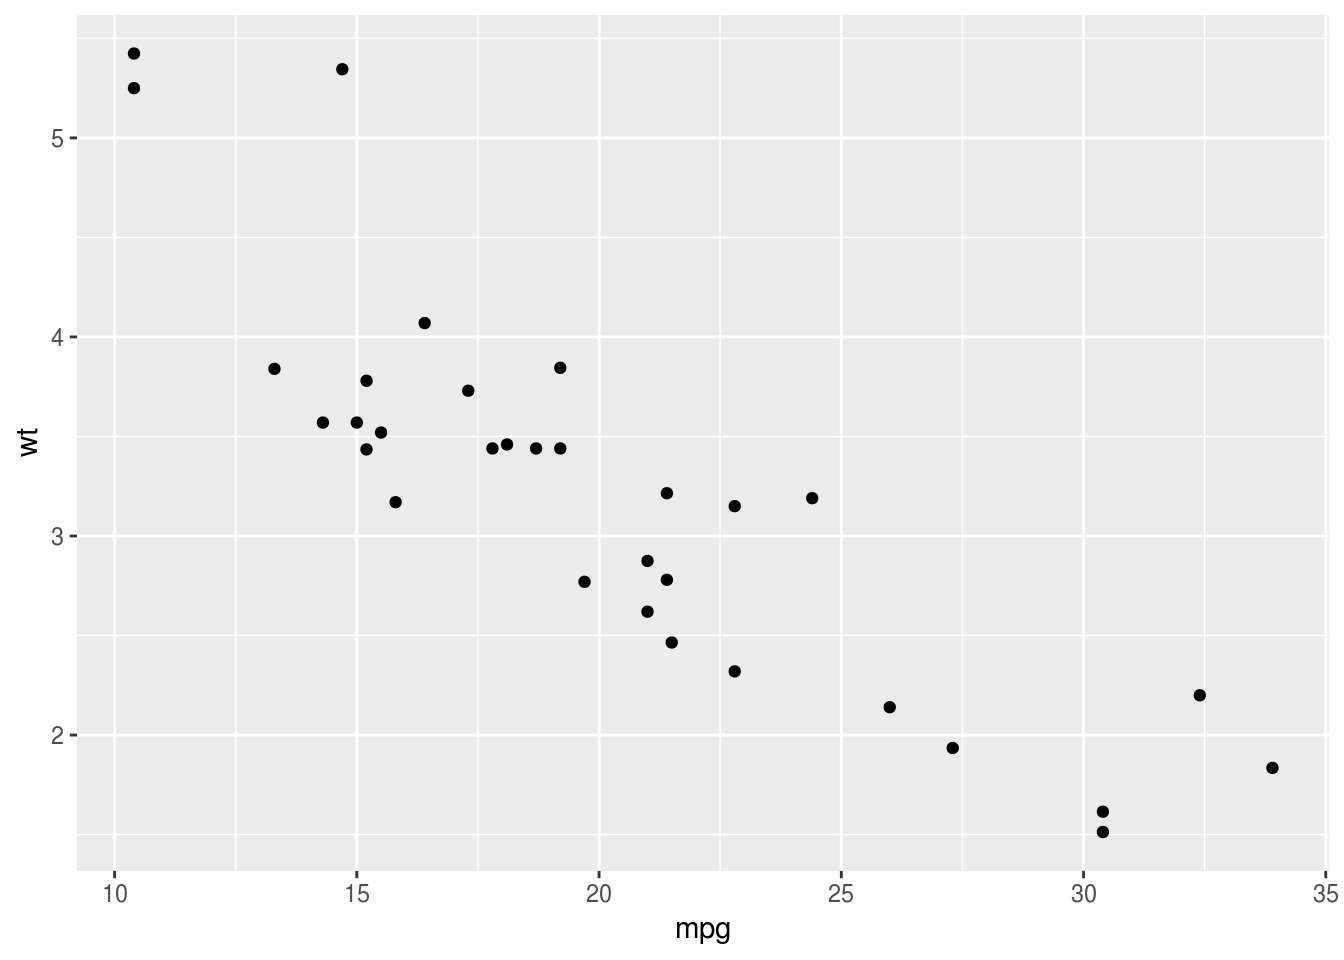
\includegraphics{graphics_files/figure-latex/unnamed-chunk-3-1.pdf}

Plotting and data visualisation is probably the best thing about R.

The base system alone provides lots of useful plotting functions, but the
\texttt{ggplot2} package is exceptional in the consistent and powerful approach it
takes to visualising data. This chapter focusses mostly on \texttt{ggplot}, but does
include some pointers to other useful plotting functions.

It's also worth pointing out here that the O'Reilly
\href{https://ase.tufts.edu/bugs/guide/assets/R\%20Graphics\%20Cookbook.pdf}{R Graphics cookbook is available as a pdf download}
and is a much more comprehensive source than this book.

The examples below are more selective and show plots likely to be of particular
use in reporting your studies.

The emphaisis on showing you how to make \emph{good} plots that help you explore data
and communicate your findings, rather than simply reproduce the output of SPSS
or Excel.

\hypertarget{graphics-benefits}{%
\subsection*{Benefits of visualising data}\label{graphics-benefits}}
\addcontentsline{toc}{subsection}{Benefits of visualising data}

Scientists attempt to understand natural processes, predict events in the
observable world, and communicate this understanding to others. In each case,
graphics are a powerful tool in their armoury.

David McCandless recently spoke at a TedX event about his work on data
journalism, and makes a persuasive case for paying more attention to
visualisations:

\hypertarget{graphics-approaches}{%
\subsection*{Which tool to use?}\label{graphics-approaches}}
\addcontentsline{toc}{subsection}{Which tool to use?}

When plotting data it pays to decide if you need:

\begin{enumerate}
\def\labelenumi{\arabic{enumi}.}
\item
  A quick way to visualise something specific -- for example to check some
  feature of your data before you continue your analysis.
\item
  A plot that is specifically designed to communicate your data effectively,
  and where you care about the details of the final output.
\end{enumerate}

For the first case --- for example to visualise a distribution of a single
variable, or to check diagnostics from a linear model --- there are lots of
useful built-in functions in base-R and other packages.

For the second case --- for example where you want to visualise the main
outcomes of your study, or draw attention to specific aspects of your data ---
there is \texttt{ggplot2}.

We case 2 first, because using ggplot highlights many important aspects of
plotting in general.

\hypertarget{layered-graphics}{%
\subsection*{\texorpdfstring{Layered graphics with \texttt{ggplot}}{Layered graphics with ggplot}}\label{layered-graphics}}
\addcontentsline{toc}{subsection}{Layered graphics with \texttt{ggplot}}

If you've never given much thought to data visualisation before, you might be
surprised at the sheer variety of graphs types available.

One way to cut through the multitude of options is to determine what the purpose
of your plot is. Although not a complete list, it's likely your plot will show
at least one of:

\begin{itemize}
\tightlist
\item
  Relationships
\item
  Distributions
\item
  Comparison
\item
  Composition
\end{itemize}

The \texttt{ggplot} library makes it easy to produce high quality graphics which serve
these ends, and to layer them to produce information-dense plots which are
really effective forms of communication.

\begin{figure}
\centering
\includegraphics{graphics_files/figure-latex/unnamed-chunk-4-1.pdf}
\caption{\label{fig:unnamed-chunk-4}Examples of charts showing comaprisons, relationships, distribution and composition. The comparison, distribution and composition plots show 2 variables, but the relationship plot includes 3, increasing the density of the information displayed.}
\end{figure}

\hypertarget{a-thought-on-chart-chooser-guides}{%
\subsubsection*{A thought on `chart chooser' guides}\label{a-thought-on-chart-chooser-guides}}
\addcontentsline{toc}{subsubsection}{A thought on `chart chooser' guides}

There are various simple chart selection guides available online, of which these
are quite nice examples:

\begin{itemize}
\tightlist
\item
  \href{http://extremepresentation.typepad.com/blog/2006/09/choosing_a_good.html}{Chart selection guide (pdf)}
\item
  \href{https://www.perceptualedge.com/articles/misc/Graph_Selection_Matrix.pdf}{`Show me the numbers' chart guide (pdf)}
\end{itemize}

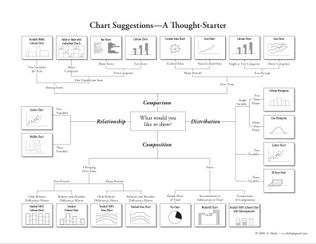
\includegraphics{media/choosing_a_good_chart.jpg}

\emph{However}, guides which attempt to be comprehensive and show you a full range of
plot types are perhaps not as useful as those which reflect our knowledge of
which plots are the most effective forms of communication.

For example, almost all guides to plotting, and especially R textbooks, will
show you how to plot a simple bar graph. But bar graphs have numerous
disadvantages over other plots which can show the same information.

Specifically, they:

\begin{itemize}
\item
  are low in information density (and so inefficient in use of space)
\item
  make comparisons between multiple data series very difficult (for example in
  \protect\hyperlink{understanding-interactions}{interaction plots}), and
\item
  perhaps most importantly, even when they include error bars, readers
  consistently misinterpret the quantitative information in bar graphs
  (specifically, when bar graphs are used to display estimates which contain
  error, readers assume points above the bar are less likely than points
  within the bar, even though this is typically not the case).
\end{itemize}

You should be guided in choosing plots not by mechanical rules based on the
number or type of variables you want to display. Instead, you should be guided
by the evidence from basic studies of human perception, and applied data on how
different types of infromation displays are really used by readers.

\textbf{This guide is restricted to examples likely to be useful and effective for
experimental and applied psychologists.}

\hypertarget{thinking-like-ggplot}{%
\subsubsection*{\texorpdfstring{Thinking like \texttt{ggplot}}{Thinking like ggplot}}\label{thinking-like-ggplot}}
\addcontentsline{toc}{subsubsection}{Thinking like \texttt{ggplot}}

When using \texttt{ggplot} it helps to think of five separate steps to making a plot (2
are optional, but commonly used):

\begin{enumerate}
\def\labelenumi{\arabic{enumi}.}
\item
  Choose the data you want to plot.
\item
  Map variables to axes or other features of the plot (e.g.~sizes or colours).
\item
  (Optionally) use \texttt{ggplot} functions to summarise your data before the plot is
  drawn (e.g.~to calulate means and standard errors for point-range plots).
\item
  Add visual display layers.
\item
  (Optionally) Split the plot up across multiple panels using groupings in the
  data.
\end{enumerate}

You can then customise the plot labels and title, and tweak other presentation
parameters, although this often isn't necessary unless sending a graphic for
publication. You can also export graphics in multiple high quality formats.

The simplest way to demonstrate these steps is with an example, and we begin
with a plot showing the relationship betwen variables:

\hypertarget{relationships}{%
\subsubsection*{`Relationships'}\label{relationships}}
\addcontentsline{toc}{subsubsection}{`Relationships'}

Problem to be solved: \emph{You want to check/show whether variables are related in a
linear fashion, e.g.~before running linear regression}

\hypertarget{step-1-select-data-to-plot}{%
\subparagraph{Step 1: Select data to plot}\label{step-1-select-data-to-plot}}
\addcontentsline{toc}{subparagraph}{Step 1: Select data to plot}

Step 1 is to select our data. As is typical in R, \texttt{ggplot} works best with
long-format data. In the examples below we will use the \texttt{mtcars} dataset for
convenience, so our first line of code is to use the \texttt{dplyr} pipe symbol
(operator) to send the \texttt{mtcars} dataset to the next line of code:

\begin{Shaded}
\begin{Highlighting}[]
\NormalTok{mtcars }\OperatorTok
\StringTok{  }\NormalTok{...}
\end{Highlighting}
\end{Shaded}

\hypertarget{step-2-map-variables-to-axes-colours-and-other-features}{%
\subparagraph{Step 2: Map variables to axes, colours, and other features}\label{step-2-map-variables-to-axes-colours-and-other-features}}
\addcontentsline{toc}{subparagraph}{Step 2: Map variables to axes, colours, and other features}

Step 2 is to map the variables we want to axes or other features of the plot
(e.g.~the colours of points, or the linetypes used in line plots).

The specify these mappings we use the \texttt{aes()} function, which is slightly
cryptic, but short for `aesthetics mapping'. Depending on the plot type you will
specify different aesthetics, and they can also have different effects depending
on the plot type, but you will commonly specify:

\begin{itemize}
\tightlist
\item
  \texttt{x} the variable to use as the x axis
\item
  \texttt{y} the variable to use as the y axis
\item
  \texttt{colour}: the variable to use to colour points or lines
\end{itemize}

Here we tell \texttt{ggplot} to use \texttt{disp} (engine size) on the x axis, and \texttt{mpg} on
the y axis. We also tell it to colour the points differently depending on the
value of \texttt{hp} (engine horsepower).

At this point \texttt{ggplot} will create and label the axes and plot area, but doesn't
yet display any of our data. For this we need to add visual display layers (in
the next step).

\begin{Shaded}
\begin{Highlighting}[]
\NormalTok{mtcars }\OperatorTok
\StringTok{  }\KeywordTok{ggplot}\NormalTok{(}\KeywordTok{aes}\NormalTok{(}\DataTypeTok{x =}\NormalTok{ disp, }\DataTypeTok{y =}\NormalTok{ mpg, }\DataTypeTok{colour=}\NormalTok{hp))}
\end{Highlighting}
\end{Shaded}

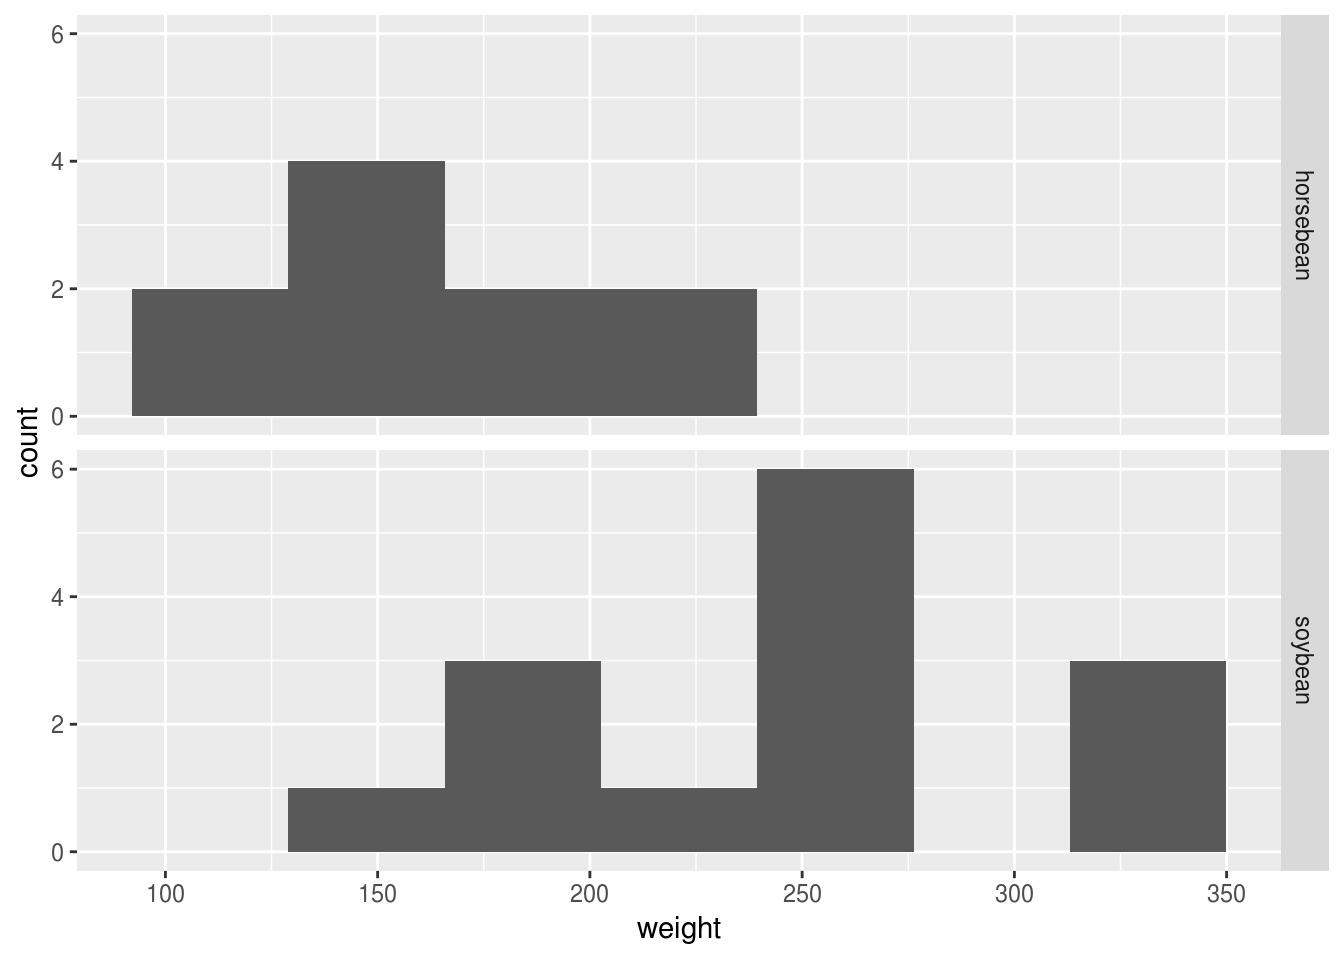
\includegraphics{graphics_files/figure-latex/unnamed-chunk-6-1.pdf}

Other aesthetics

There are many other aesthetics which can be specified. Some of the most useful
are:

\begin{itemize}
\tightlist
\item
  \texttt{ymin} and \texttt{ymax}: for upper and lower bounds, e.g.~on error bars
\item
  \texttt{group}:which tells ggplot to group observations by some variable and, for
  example, plot a different line per-group)
\item
  \texttt{fill}: like \texttt{colour} but for areas/shapes
\item
  \texttt{alpha} and \texttt{size}: control the size and opacity of visual features (useful
  for de-emphasising some features of a plot to make others stand out)
\end{itemize}

See the ggplot documentation for more details:
\url{http://ggplot2.tidyverse.org/reference/\#section-aesthetics}

\hypertarget{step-3}{%
\subparagraph{Step 3}\label{step-3}}
\addcontentsline{toc}{subparagraph}{Step 3}

We skip step 3 for this example (asking ggplot to automatically make summaries
of our data before plotting), but will cover it below - see the \texttt{stat\_summary()}
function.

\hypertarget{step-4-display-data}{%
\subparagraph{Step 4: Display data}\label{step-4-display-data}}
\addcontentsline{toc}{subparagraph}{Step 4: Display data}

To display data, we have to add a visual layer to the plot. For example, let's
say we want to make a scatter plot, and so draw points for each row of data:

\begin{Shaded}
\begin{Highlighting}[]
\NormalTok{mtcars }\OperatorTok
\StringTok{  }\KeywordTok{ggplot}\NormalTok{(}\KeywordTok{aes}\NormalTok{(}\DataTypeTok{x =}\NormalTok{ disp, }\DataTypeTok{y =}\NormalTok{ mpg, }\DataTypeTok{colour=}\NormalTok{hp)) }\OperatorTok{+}
\StringTok{  }\KeywordTok{geom_point}\NormalTok{()}
\end{Highlighting}
\end{Shaded}

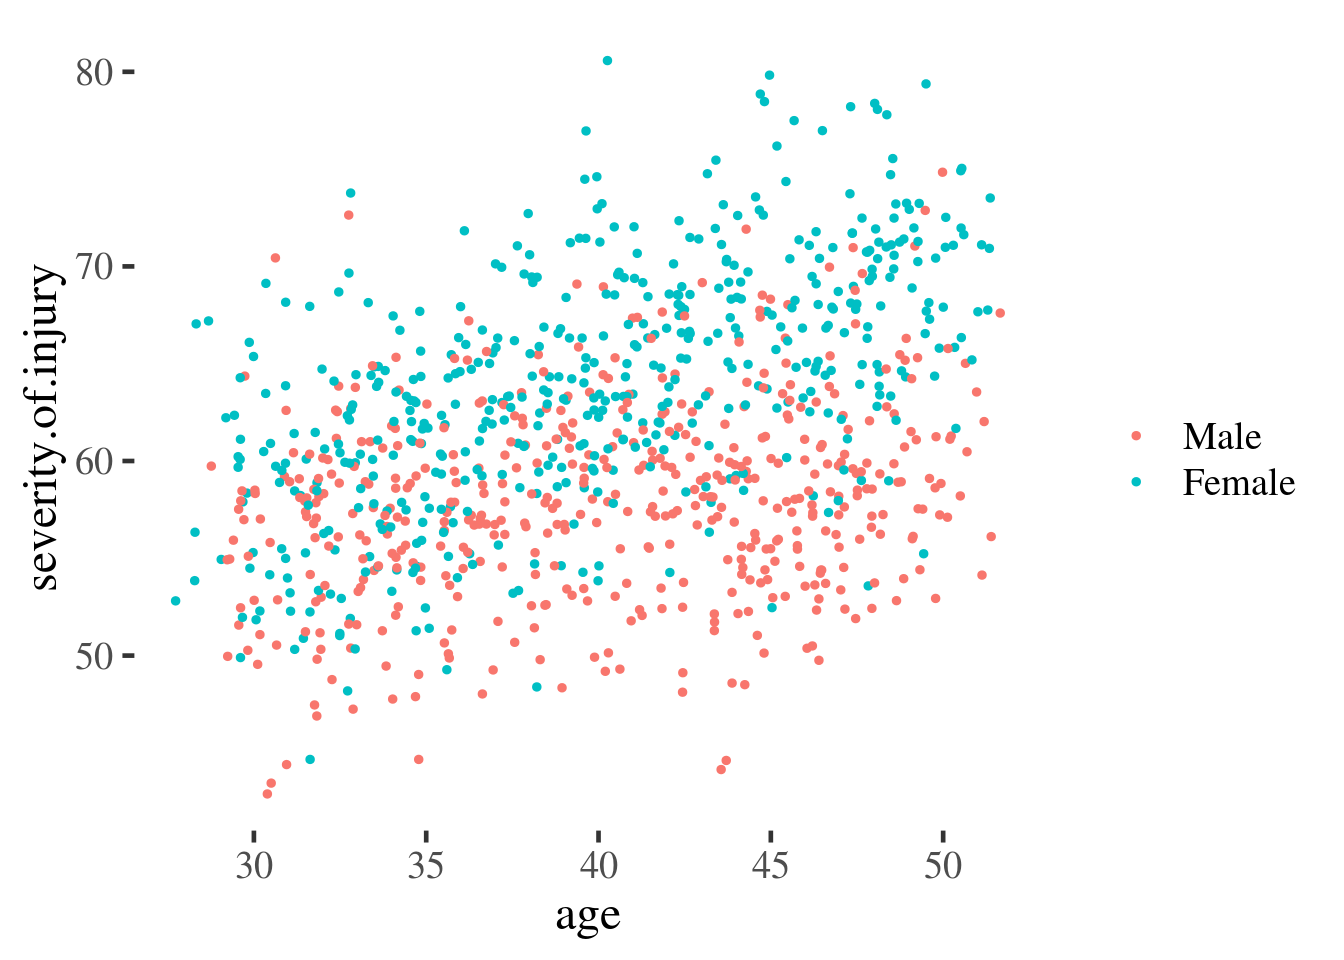
\includegraphics{graphics_files/figure-latex/unnamed-chunk-7-1.pdf}

And we have a pretty slick graph: \texttt{ggplot} has now added points for each pair of
\texttt{disp} and \texttt{mpg} values, and coloured them according to the value of \texttt{hp} (see
\protect\hyperlink{picking-colours}{choosing colours below}).

{Use the \texttt{airquality} dataset and create your own scatterplot and try to colour
the points using the \texttt{Month} variable. Should \texttt{Month} be used as a factor or a
numeric variable when colouring the points?}

What's even neater about \texttt{ggplot} though is how easy it is to \emph{layer} different
visualisations of the same data. These visual layers are called \texttt{geom}'s and the
functions which add them are all prefixed with \texttt{geom\_}, so \texttt{geom\_point()} for
scatter plots, or \texttt{geom\_line()} for line plots, or \texttt{geom\_smooth()} for a
smoothed line plot. We can add this to the scatter plot like so:

\begin{Shaded}
\begin{Highlighting}[]
\NormalTok{mtcars }\OperatorTok
\StringTok{  }\KeywordTok{ggplot}\NormalTok{(}\KeywordTok{aes}\NormalTok{(}\DataTypeTok{x =}\NormalTok{ disp, }\DataTypeTok{y =}\NormalTok{ mpg, }\DataTypeTok{colour=}\NormalTok{hp)) }\OperatorTok{+}
\StringTok{  }\KeywordTok{geom_point}\NormalTok{(}\DataTypeTok{size=}\DecValTok{2}\NormalTok{) }\OperatorTok{+}
\StringTok{  }\KeywordTok{geom_smooth}\NormalTok{(}\DataTypeTok{se=}\NormalTok{F, }\DataTypeTok{colour=}\StringTok{"grey"}\NormalTok{)}
\end{Highlighting}
\end{Shaded}

\includegraphics{graphics_files/figure-latex/unnamed-chunk-9-1.pdf}

In the example above, I have also customised the smoothed line, making it grey
to avoid over-intrusion into our perception of the points. Often less is more
when plotting graphs: not everything can be emphasised at once, and \emph{it's
important to make decisions about what should be given visual priority}.

\hypertarget{step-5-splitting-up-or-repeating-the-plot.}{%
\subparagraph{Step 5: `Splitting up' or repeating the plot.}\label{step-5-splitting-up-or-repeating-the-plot.}}
\addcontentsline{toc}{subparagraph}{Step 5: `Splitting up' or repeating the plot.}

Very often, you will have drawn plot and think things like \emph{I wonder what that
would look like if I drew it for men and women separately?}. In \texttt{ggplot} this is
called facetting, and is easy to achieve, provided your data are in a long
format.

Using the same \texttt{mtcars} example, let's say we wanted separate panels for
American vs.~Foreign cars (information held in the \texttt{am} variable). We simply add
the \texttt{facet\_wrap()}, and specify the \texttt{"am"} variable:

\begin{Shaded}
\begin{Highlighting}[]
\NormalTok{mtcars }\OperatorTok
\StringTok{  }\KeywordTok{ggplot}\NormalTok{(}\KeywordTok{aes}\NormalTok{(}\DataTypeTok{x =}\NormalTok{ disp, }\DataTypeTok{y =}\NormalTok{ mpg, }\DataTypeTok{colour=}\NormalTok{hp)) }\OperatorTok{+}
\StringTok{  }\KeywordTok{geom_point}\NormalTok{(}\DataTypeTok{size=}\DecValTok{2}\NormalTok{) }\OperatorTok{+}
\StringTok{  }\KeywordTok{geom_smooth}\NormalTok{(}\DataTypeTok{se=}\NormalTok{F, }\DataTypeTok{colour=}\StringTok{"grey"}\NormalTok{) }\OperatorTok{+}
\StringTok{  }\KeywordTok{facet_wrap}\NormalTok{(}\StringTok{"am"}\NormalTok{)}
\end{Highlighting}
\end{Shaded}

\includegraphics{graphics_files/figure-latex/unnamed-chunk-10-1.pdf}

One trick is to make sure factors are labelled nicely, because these labels
appear on the final plot. Here the \texttt{mutate()} call
\href{real-data.html\#factors-and-numerics}{relabels the factor} which makes the plot
easier to read:

\begin{Shaded}
\begin{Highlighting}[]
\NormalTok{mtcars }\OperatorTok
\StringTok{  }\KeywordTok{mutate}\NormalTok{(}\DataTypeTok{american =} \KeywordTok{factor}\NormalTok{(am, }\DataTypeTok{labels=}\KeywordTok{c}\NormalTok{(}\StringTok{"American"}\NormalTok{, }\StringTok{"Foreign"}\NormalTok{))) }\OperatorTok
\StringTok{  }\KeywordTok{ggplot}\NormalTok{(}\KeywordTok{aes}\NormalTok{(}\DataTypeTok{x =}\NormalTok{ disp, }\DataTypeTok{y =}\NormalTok{ mpg, }\DataTypeTok{colour=}\NormalTok{hp)) }\OperatorTok{+}
\StringTok{  }\KeywordTok{geom_point}\NormalTok{(}\DataTypeTok{size=}\DecValTok{2}\NormalTok{) }\OperatorTok{+}
\StringTok{  }\KeywordTok{geom_smooth}\NormalTok{(}\DataTypeTok{se=}\NormalTok{F, }\DataTypeTok{colour=}\StringTok{"grey"}\NormalTok{) }\OperatorTok{+}
\StringTok{  }\KeywordTok{facet_wrap}\NormalTok{(}\StringTok{"american"}\NormalTok{)}
\end{Highlighting}
\end{Shaded}

\includegraphics{graphics_files/figure-latex/unnamed-chunk-11-1.pdf}

\href{http://ggplot2.tidyverse.org/reference/\#section-facetting}{See the ggplot documentation on facetting for more details}.

\hypertarget{distributions}{%
\subsubsection*{`Distributions'}\label{distributions}}
\addcontentsline{toc}{subsubsection}{`Distributions'}

\begin{Shaded}
\begin{Highlighting}[]
\NormalTok{lme4}\OperatorTok{::}\NormalTok{sleepstudy }\OperatorTok
\StringTok{  }\KeywordTok{ggplot}\NormalTok{(}\KeywordTok{aes}\NormalTok{(Reaction)) }\OperatorTok{+}\StringTok{ }\KeywordTok{geom_density}\NormalTok{()}
\end{Highlighting}
\end{Shaded}

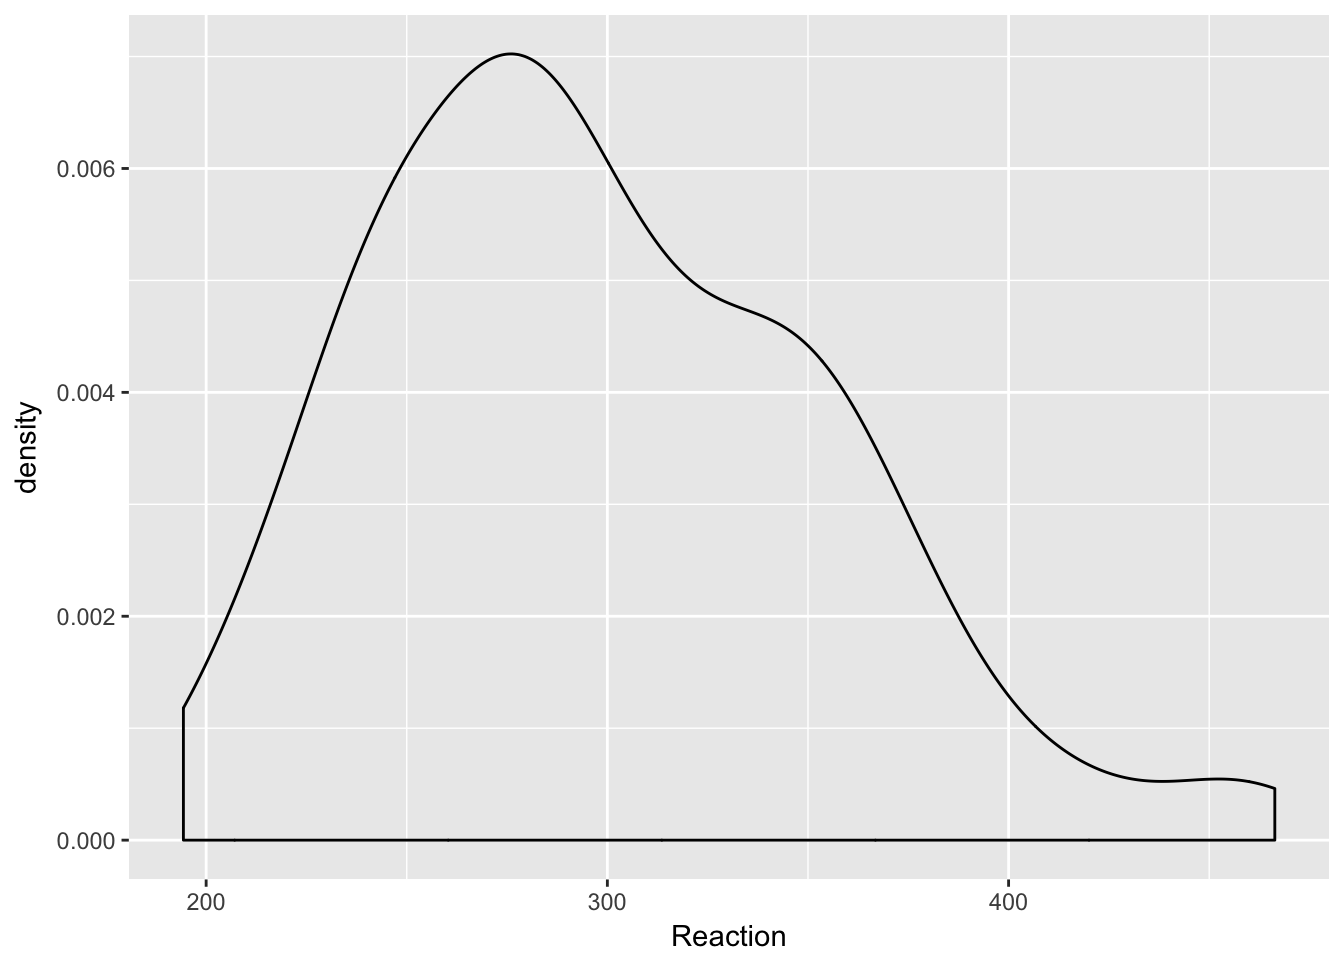
\includegraphics{graphics_files/figure-latex/unnamed-chunk-12-1.pdf}

Imagine we wanted to compare distributions for individuals. Simply overlaying
the lines is confusing:

\begin{Shaded}
\begin{Highlighting}[]
\NormalTok{lme4}\OperatorTok{::}\NormalTok{sleepstudy }\OperatorTok
\StringTok{  }\KeywordTok{ggplot}\NormalTok{(}\KeywordTok{aes}\NormalTok{(Reaction, }\DataTypeTok{group=}\NormalTok{Subject)) }\OperatorTok{+}\StringTok{ }\KeywordTok{geom_density}\NormalTok{()}
\end{Highlighting}
\end{Shaded}

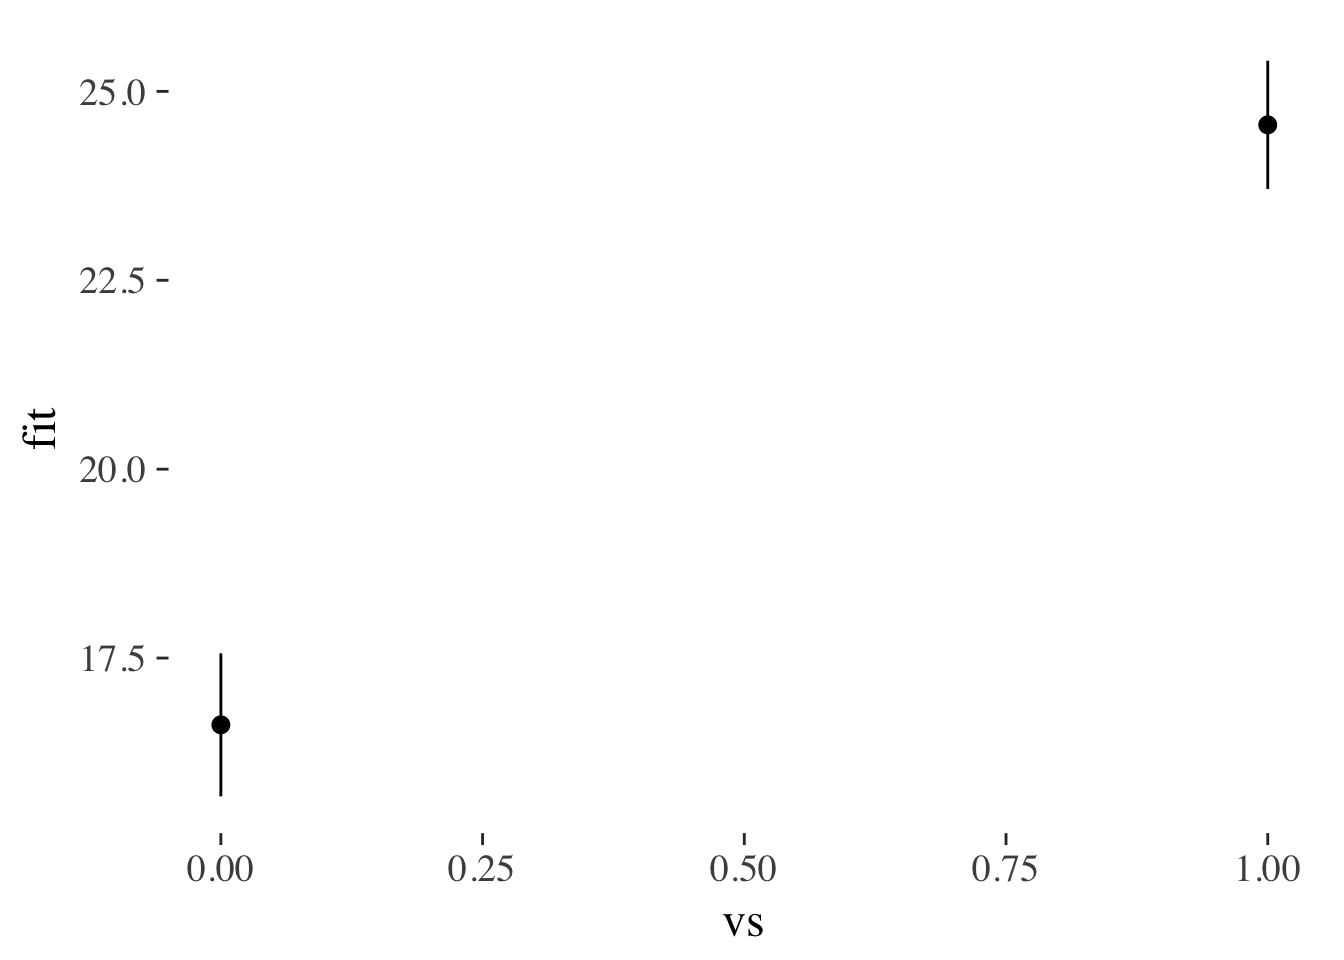
\includegraphics{graphics_files/figure-latex/unnamed-chunk-13-1.pdf}

Facetting produces a nicer result:

\begin{Shaded}
\begin{Highlighting}[]
\NormalTok{lme4}\OperatorTok{::}\NormalTok{sleepstudy }\OperatorTok
\StringTok{  }\KeywordTok{ggplot}\NormalTok{(}\KeywordTok{aes}\NormalTok{(Reaction)) }\OperatorTok{+}\StringTok{ }\KeywordTok{geom_density}\NormalTok{() }\OperatorTok{+}\StringTok{ }\KeywordTok{facet_wrap}\NormalTok{(}\StringTok{"Subject"}\NormalTok{)}
\end{Highlighting}
\end{Shaded}

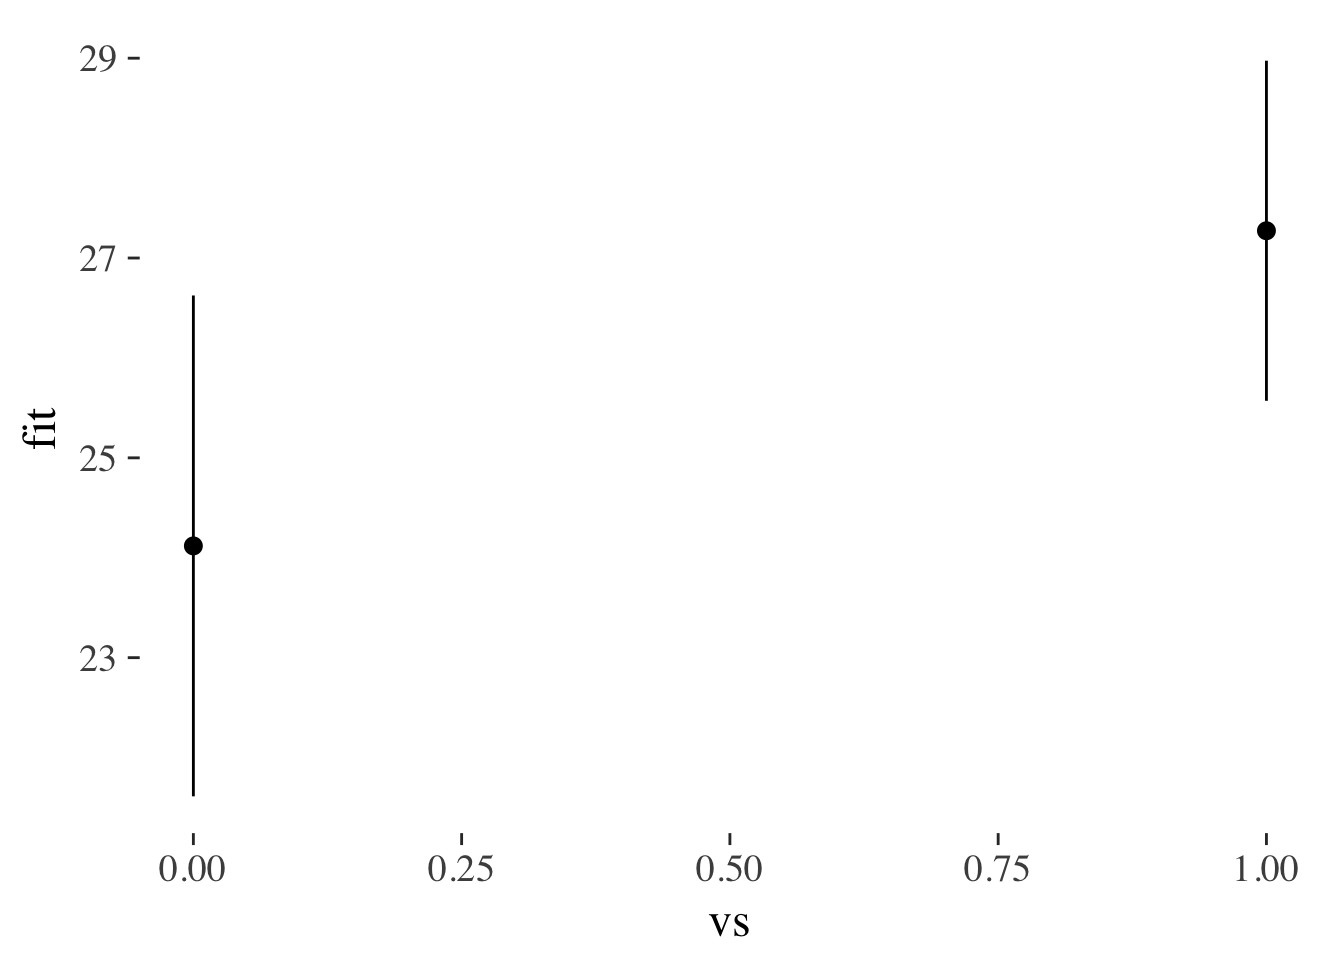
\includegraphics{graphics_files/figure-latex/unnamed-chunk-14-1.pdf}

But we could present the same information more compactly, and with better
facility to compare between subjects, if we use a bottleplot:

\begin{Shaded}
\begin{Highlighting}[]
\NormalTok{lme4}\OperatorTok{::}\NormalTok{sleepstudy }\OperatorTok
\StringTok{  }\KeywordTok{ggplot}\NormalTok{(}\KeywordTok{aes}\NormalTok{(Subject, Reaction)) }\OperatorTok{+}
\StringTok{  }\KeywordTok{geom_violin}\NormalTok{()}
\end{Highlighting}
\end{Shaded}

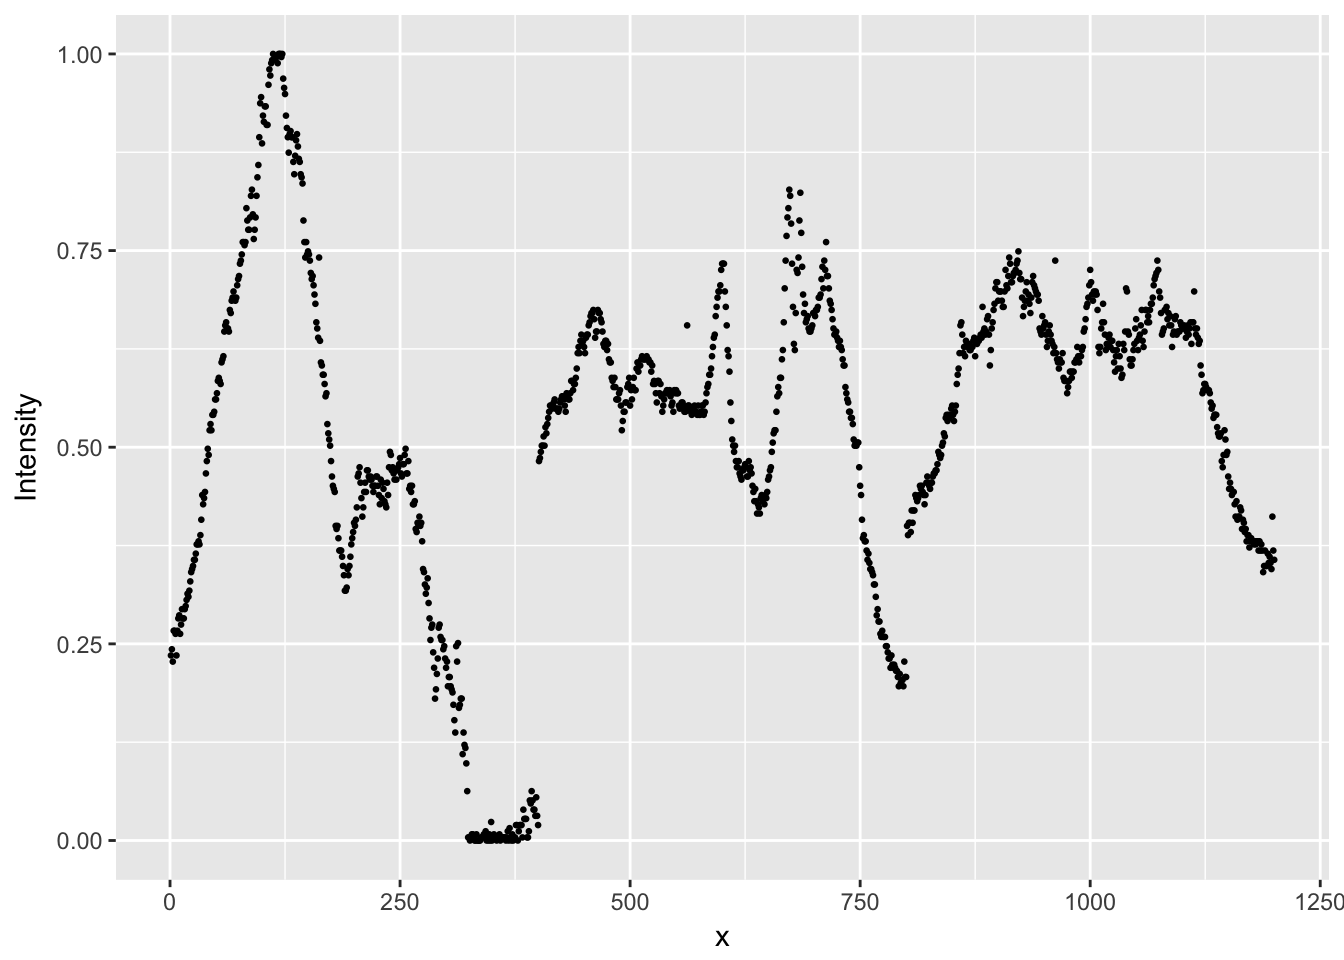
\includegraphics{graphics_files/figure-latex/unnamed-chunk-15-1.pdf}

We might want to plot our Subjects in order of their mean RT:

\begin{Shaded}
\begin{Highlighting}[]
\NormalTok{mean.ranked.sleep <-}\StringTok{ }\NormalTok{lme4}\OperatorTok{::}\NormalTok{sleepstudy }\OperatorTok
\StringTok{  }\KeywordTok{group_by}\NormalTok{(Subject) }\OperatorTok
\StringTok{  }\CommentTok{# calculate mean RT}
\StringTok{  }\KeywordTok{mutate}\NormalTok{(}\DataTypeTok{RTm =} \KeywordTok{mean}\NormalTok{(Reaction)) }\OperatorTok
\StringTok{  }\CommentTok{# sort by mean RT}
\StringTok{  }\KeywordTok{arrange}\NormalTok{(RTm, Days) }\OperatorTok
\StringTok{  }\KeywordTok{ungroup}\NormalTok{() }\OperatorTok
\StringTok{  }\CommentTok{# create a rank score but conert to factor right away}
\StringTok{  }\KeywordTok{mutate}\NormalTok{(}\DataTypeTok{SubjectRank =} \KeywordTok{factor}\NormalTok{(}\KeywordTok{dense_rank}\NormalTok{(RTm)))}

\NormalTok{mean.ranked.sleep }\OperatorTok
\StringTok{  }\KeywordTok{ggplot}\NormalTok{(}\KeywordTok{aes}\NormalTok{(SubjectRank, Reaction)) }\OperatorTok{+}
\StringTok{  }\KeywordTok{geom_violin}\NormalTok{() }\OperatorTok{+}
\StringTok{  }\KeywordTok{theme}\NormalTok{(}\DataTypeTok{aspect.ratio =} \FloatTok{.33}\NormalTok{)  }\CommentTok{# change the aspect ratio to make long and wide}
\end{Highlighting}
\end{Shaded}

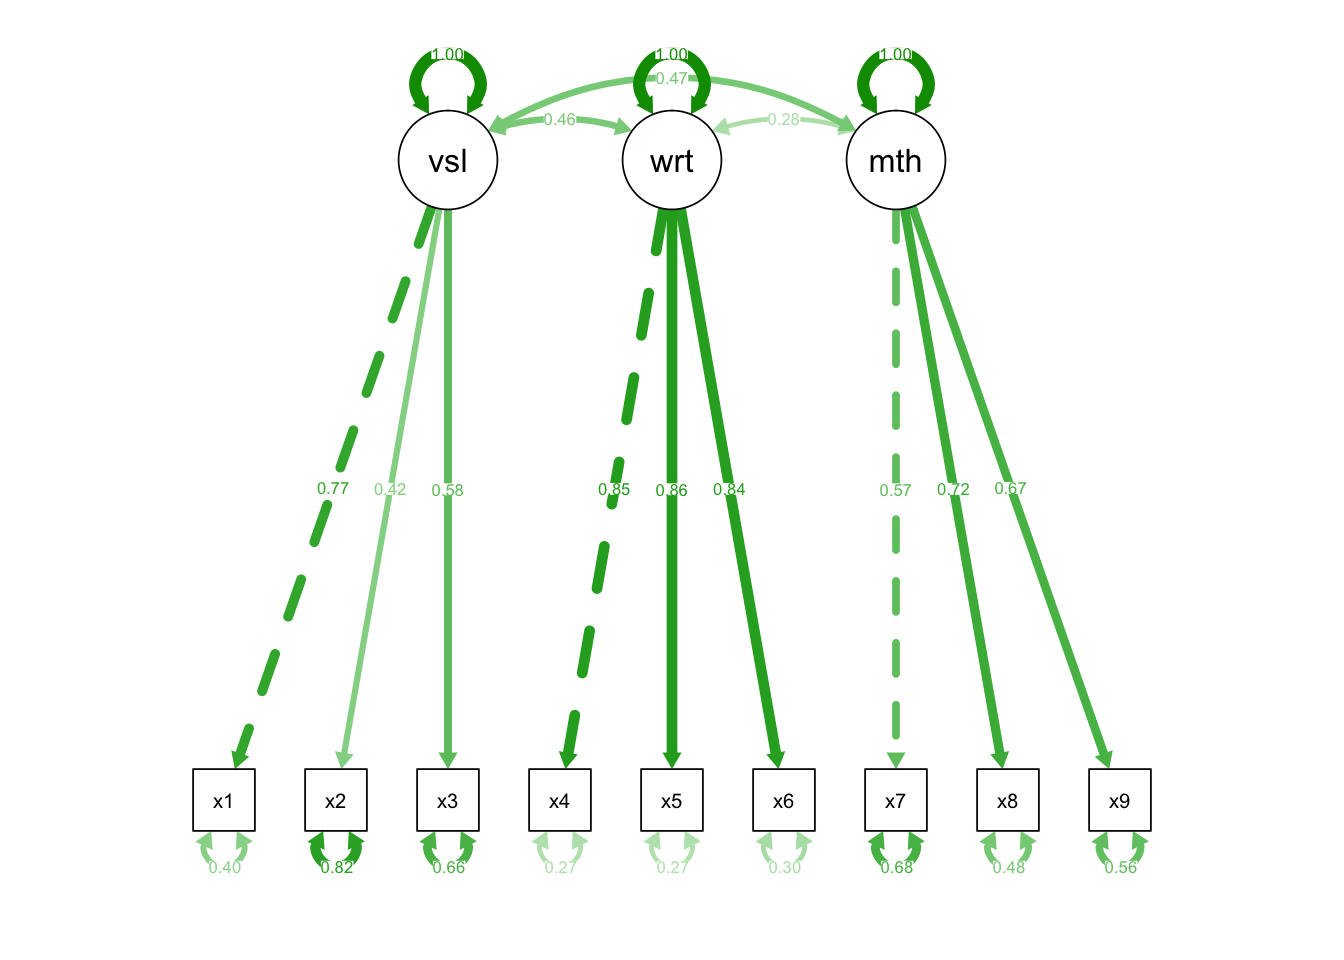
\includegraphics{graphics_files/figure-latex/unnamed-chunk-16-1.pdf}

Or we might want to compare individuals against the combined distribution:

\begin{Shaded}
\begin{Highlighting}[]
\CommentTok{# duplicate all the data, assigning one-replication to a single subject, "All"}
\NormalTok{sleep.repeat <-}\StringTok{ }\KeywordTok{bind_rows}\NormalTok{(lme4}\OperatorTok{::}\NormalTok{sleepstudy,}
\NormalTok{                          lme4}\OperatorTok{::}\NormalTok{sleepstudy }\OperatorTok\StringTok{ }\KeywordTok{mutate}\NormalTok{(}\DataTypeTok{Subject=}\StringTok{"All"}\NormalTok{))}
\NormalTok{Warning }\ControlFlowTok{in} \KeywordTok{bind_rows_}\NormalTok{(x, .id)}\OperatorTok{:}\StringTok{ }\NormalTok{binding factor and character vector,}
\NormalTok{coercing into character vector}
\NormalTok{Warning }\ControlFlowTok{in} \KeywordTok{bind_rows_}\NormalTok{(x, .id)}\OperatorTok{:}\StringTok{ }\NormalTok{binding character and factor vector,}
\NormalTok{coercing into character vector}

\NormalTok{sleep.repeat }\OperatorTok
\StringTok{  }\KeywordTok{mutate}\NormalTok{(}\DataTypeTok{all =}\NormalTok{ Subject}\OperatorTok{==}\StringTok{"All"}\NormalTok{) }\OperatorTok
\StringTok{  }\KeywordTok{ggplot}\NormalTok{(}\KeywordTok{aes}\NormalTok{(Subject, Reaction, }\DataTypeTok{color=}\NormalTok{all)) }\OperatorTok{+}
\StringTok{  }\KeywordTok{geom_violin}\NormalTok{() }\OperatorTok{+}
\StringTok{  }\KeywordTok{guides}\NormalTok{(}\DataTypeTok{colour=}\OtherTok{FALSE}\NormalTok{) }\OperatorTok{+}\StringTok{ }\CommentTok{# turn off he legend because we don't really need it}
\StringTok{  }\KeywordTok{theme}\NormalTok{(}\DataTypeTok{aspect.ratio =} \FloatTok{.25}\NormalTok{)  }\CommentTok{# change the aspect ratio to make long and wide}
\end{Highlighting}
\end{Shaded}

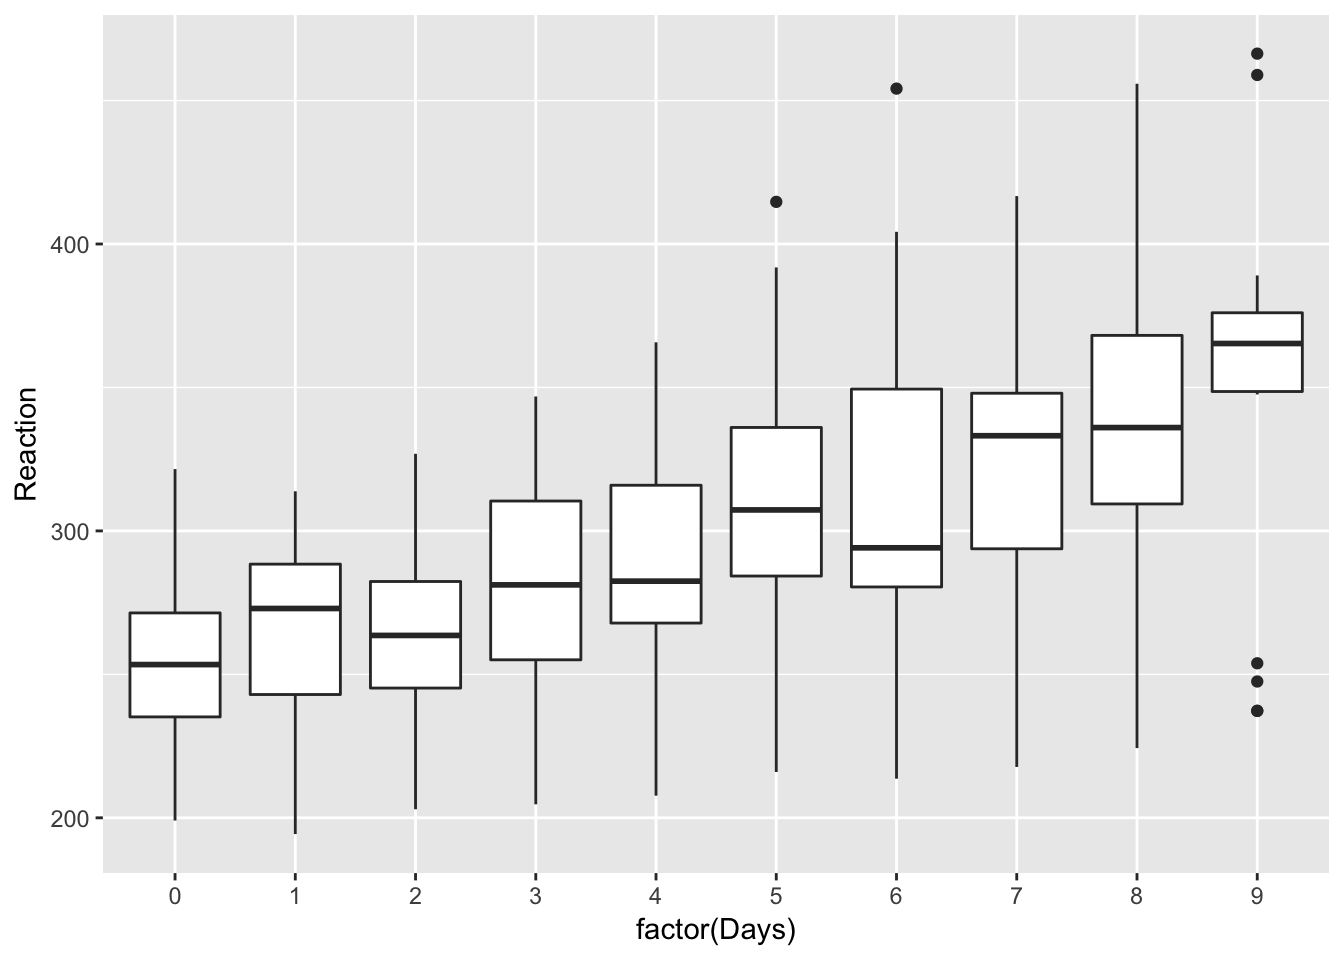
\includegraphics{graphics_files/figure-latex/unnamed-chunk-17-1.pdf}

Boxplots can also work well to show distributions, and have the advantage of
showing the median explicitly:

\begin{Shaded}
\begin{Highlighting}[]
\NormalTok{mean.ranked.sleep }\OperatorTok
\StringTok{  }\KeywordTok{ggplot}\NormalTok{(}\KeywordTok{aes}\NormalTok{(SubjectRank, Reaction)) }\OperatorTok{+}
\StringTok{  }\KeywordTok{geom_boxplot}\NormalTok{()}
\end{Highlighting}
\end{Shaded}

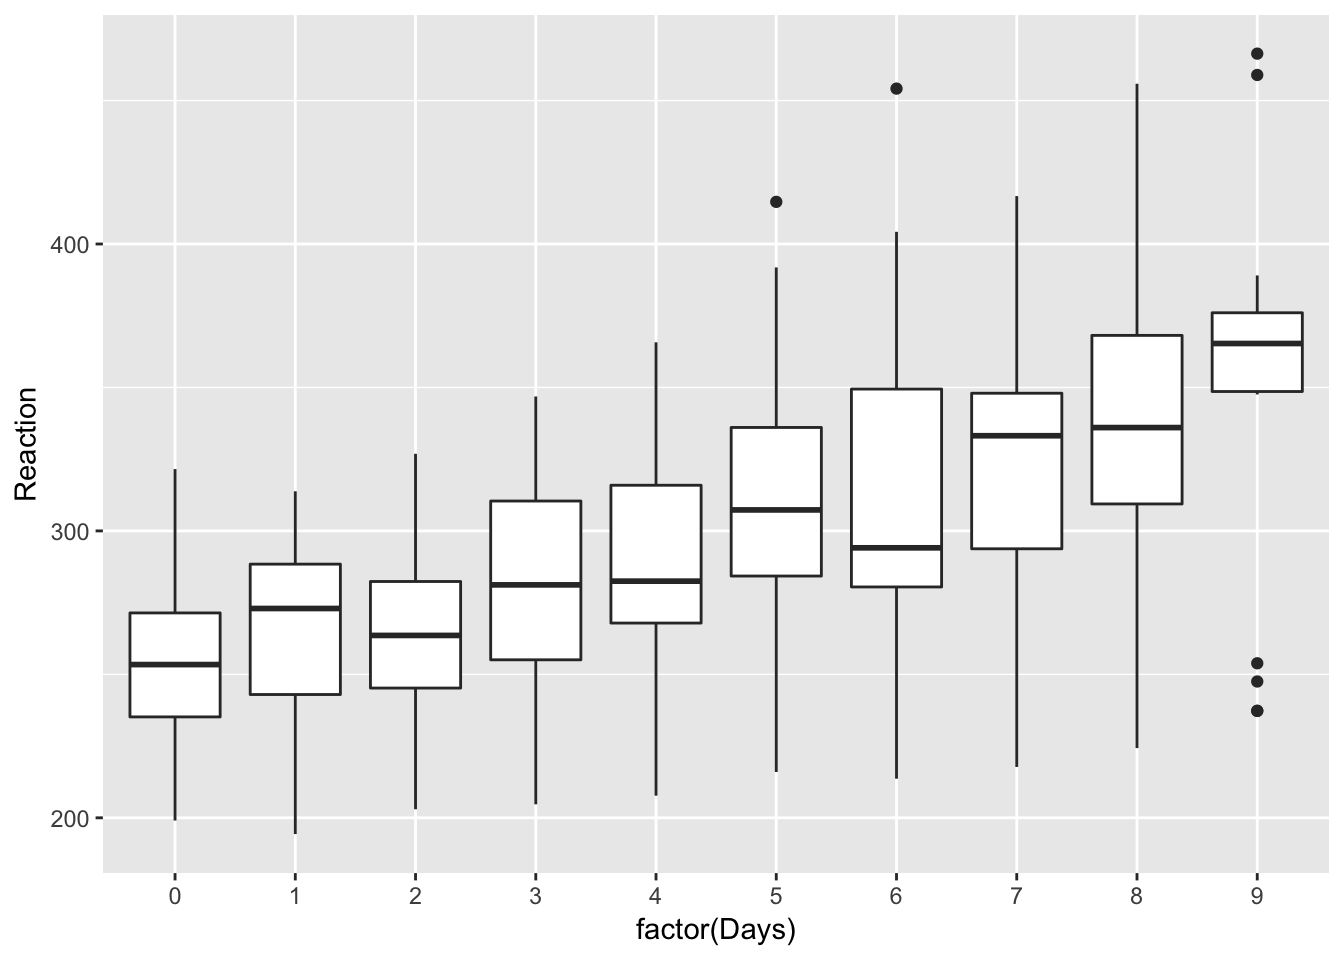
\includegraphics{graphics_files/figure-latex/unnamed-chunk-18-1.pdf}

If we plot the same data by-day, we can clearly see the effect of sleep
deprivation, and the increase in variability between subjects as sime goes on:
the lack of sleeps seems to be affecting some subjects more than others

\begin{Shaded}
\begin{Highlighting}[]
\NormalTok{lme4}\OperatorTok{::}\NormalTok{sleepstudy }\OperatorTok
\StringTok{  }\KeywordTok{ggplot}\NormalTok{(}\KeywordTok{aes}\NormalTok{(}\KeywordTok{factor}\NormalTok{(Days), Reaction)) }\OperatorTok{+}
\StringTok{  }\KeywordTok{geom_boxplot}\NormalTok{()}
\end{Highlighting}
\end{Shaded}

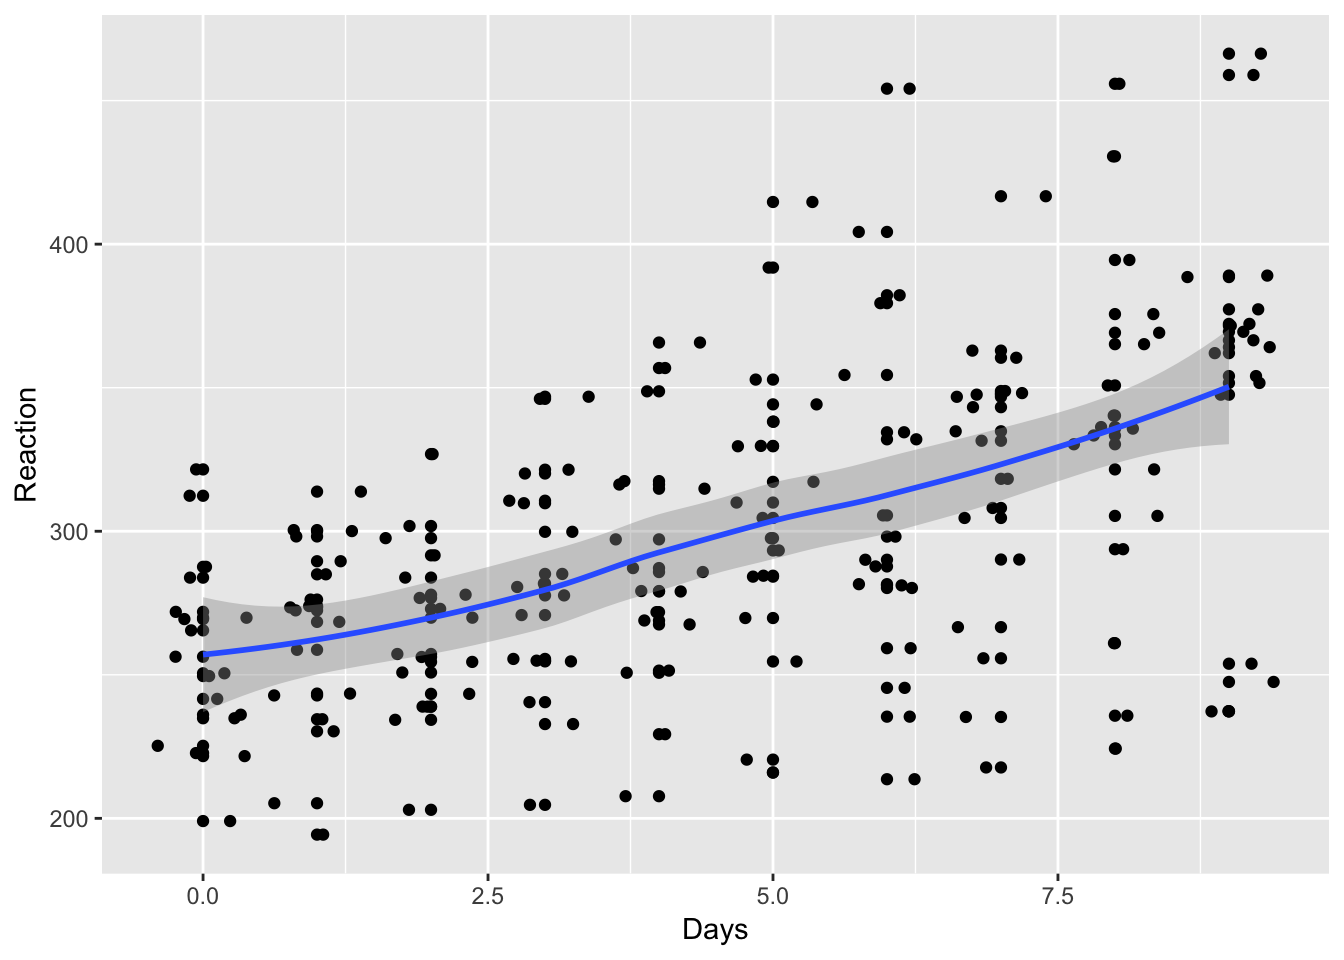
\includegraphics{graphics_files/figure-latex/unnamed-chunk-19-1.pdf}

\hypertarget{comparisons}{%
\subsubsection*{`Comparisons'}\label{comparisons}}
\addcontentsline{toc}{subsubsection}{`Comparisons'}

Imagine we have rainfall and temperature data for various regions, across
months:

\begin{Shaded}
\begin{Highlighting}[]
\NormalTok{DAAG}\OperatorTok{::}\NormalTok{bomregions }\OperatorTok
\StringTok{  }\NormalTok{psych}\OperatorTok{::}\KeywordTok{describe}\NormalTok{(}\DataTypeTok{fast=}\NormalTok{T) }\OperatorTok
\StringTok{  }\NormalTok{pander}
\end{Highlighting}
\end{Shaded}

\begin{longtable}[]{@{}ccccccccc@{}}
\toprule
\begin{minipage}[b]{0.14\columnwidth}\centering
~\strut
\end{minipage} & \begin{minipage}[b]{0.06\columnwidth}\centering
vars\strut
\end{minipage} & \begin{minipage}[b]{0.05\columnwidth}\centering
n\strut
\end{minipage} & \begin{minipage}[b]{0.11\columnwidth}\centering
mean\strut
\end{minipage} & \begin{minipage}[b]{0.08\columnwidth}\centering
sd\strut
\end{minipage} & \begin{minipage}[b]{0.08\columnwidth}\centering
min\strut
\end{minipage} & \begin{minipage}[b]{0.07\columnwidth}\centering
max\strut
\end{minipage} & \begin{minipage}[b]{0.07\columnwidth}\centering
range\strut
\end{minipage} & \begin{minipage}[b]{0.09\columnwidth}\centering
se\strut
\end{minipage}\tabularnewline
\midrule
\endhead
\begin{minipage}[t]{0.14\columnwidth}\centering
\textbf{Year}\strut
\end{minipage} & \begin{minipage}[t]{0.06\columnwidth}\centering
1\strut
\end{minipage} & \begin{minipage}[t]{0.05\columnwidth}\centering
109\strut
\end{minipage} & \begin{minipage}[t]{0.11\columnwidth}\centering
1954\strut
\end{minipage} & \begin{minipage}[t]{0.08\columnwidth}\centering
31.61\strut
\end{minipage} & \begin{minipage}[t]{0.08\columnwidth}\centering
1900\strut
\end{minipage} & \begin{minipage}[t]{0.07\columnwidth}\centering
2008\strut
\end{minipage} & \begin{minipage}[t]{0.07\columnwidth}\centering
108\strut
\end{minipage} & \begin{minipage}[t]{0.09\columnwidth}\centering
3.028\strut
\end{minipage}\tabularnewline
\begin{minipage}[t]{0.14\columnwidth}\centering
\textbf{eastAVt}\strut
\end{minipage} & \begin{minipage}[t]{0.06\columnwidth}\centering
2\strut
\end{minipage} & \begin{minipage}[t]{0.05\columnwidth}\centering
99\strut
\end{minipage} & \begin{minipage}[t]{0.11\columnwidth}\centering
20.43\strut
\end{minipage} & \begin{minipage}[t]{0.08\columnwidth}\centering
0.4585\strut
\end{minipage} & \begin{minipage}[t]{0.08\columnwidth}\centering
19.35\strut
\end{minipage} & \begin{minipage}[t]{0.07\columnwidth}\centering
21.61\strut
\end{minipage} & \begin{minipage}[t]{0.07\columnwidth}\centering
2.255\strut
\end{minipage} & \begin{minipage}[t]{0.09\columnwidth}\centering
0.04608\strut
\end{minipage}\tabularnewline
\begin{minipage}[t]{0.14\columnwidth}\centering
\textbf{seAVt}\strut
\end{minipage} & \begin{minipage}[t]{0.06\columnwidth}\centering
3\strut
\end{minipage} & \begin{minipage}[t]{0.05\columnwidth}\centering
99\strut
\end{minipage} & \begin{minipage}[t]{0.11\columnwidth}\centering
14.59\strut
\end{minipage} & \begin{minipage}[t]{0.08\columnwidth}\centering
0.4547\strut
\end{minipage} & \begin{minipage}[t]{0.08\columnwidth}\centering
13.62\strut
\end{minipage} & \begin{minipage}[t]{0.07\columnwidth}\centering
15.94\strut
\end{minipage} & \begin{minipage}[t]{0.07\columnwidth}\centering
2.32\strut
\end{minipage} & \begin{minipage}[t]{0.09\columnwidth}\centering
0.0457\strut
\end{minipage}\tabularnewline
\begin{minipage}[t]{0.14\columnwidth}\centering
\textbf{southAVt}\strut
\end{minipage} & \begin{minipage}[t]{0.06\columnwidth}\centering
4\strut
\end{minipage} & \begin{minipage}[t]{0.05\columnwidth}\centering
99\strut
\end{minipage} & \begin{minipage}[t]{0.11\columnwidth}\centering
18.48\strut
\end{minipage} & \begin{minipage}[t]{0.08\columnwidth}\centering
0.4584\strut
\end{minipage} & \begin{minipage}[t]{0.08\columnwidth}\centering
17.43\strut
\end{minipage} & \begin{minipage}[t]{0.07\columnwidth}\centering
19.53\strut
\end{minipage} & \begin{minipage}[t]{0.07\columnwidth}\centering
2.1\strut
\end{minipage} & \begin{minipage}[t]{0.09\columnwidth}\centering
0.04607\strut
\end{minipage}\tabularnewline
\begin{minipage}[t]{0.14\columnwidth}\centering
\textbf{swAVt}\strut
\end{minipage} & \begin{minipage}[t]{0.06\columnwidth}\centering
5\strut
\end{minipage} & \begin{minipage}[t]{0.05\columnwidth}\centering
99\strut
\end{minipage} & \begin{minipage}[t]{0.11\columnwidth}\centering
16.18\strut
\end{minipage} & \begin{minipage}[t]{0.08\columnwidth}\centering
0.4734\strut
\end{minipage} & \begin{minipage}[t]{0.08\columnwidth}\centering
15.08\strut
\end{minipage} & \begin{minipage}[t]{0.07\columnwidth}\centering
17.05\strut
\end{minipage} & \begin{minipage}[t]{0.07\columnwidth}\centering
1.97\strut
\end{minipage} & \begin{minipage}[t]{0.09\columnwidth}\centering
0.04758\strut
\end{minipage}\tabularnewline
\begin{minipage}[t]{0.14\columnwidth}\centering
\textbf{westAVt}\strut
\end{minipage} & \begin{minipage}[t]{0.06\columnwidth}\centering
6\strut
\end{minipage} & \begin{minipage}[t]{0.05\columnwidth}\centering
99\strut
\end{minipage} & \begin{minipage}[t]{0.11\columnwidth}\centering
22.33\strut
\end{minipage} & \begin{minipage}[t]{0.08\columnwidth}\centering
0.4548\strut
\end{minipage} & \begin{minipage}[t]{0.08\columnwidth}\centering
21.22\strut
\end{minipage} & \begin{minipage}[t]{0.07\columnwidth}\centering
23.39\strut
\end{minipage} & \begin{minipage}[t]{0.07\columnwidth}\centering
2.165\strut
\end{minipage} & \begin{minipage}[t]{0.09\columnwidth}\centering
0.04571\strut
\end{minipage}\tabularnewline
\begin{minipage}[t]{0.14\columnwidth}\centering
\textbf{northAVt}\strut
\end{minipage} & \begin{minipage}[t]{0.06\columnwidth}\centering
7\strut
\end{minipage} & \begin{minipage}[t]{0.05\columnwidth}\centering
99\strut
\end{minipage} & \begin{minipage}[t]{0.11\columnwidth}\centering
24.6\strut
\end{minipage} & \begin{minipage}[t]{0.08\columnwidth}\centering
0.5042\strut
\end{minipage} & \begin{minipage}[t]{0.08\columnwidth}\centering
23.57\strut
\end{minipage} & \begin{minipage}[t]{0.07\columnwidth}\centering
25.94\strut
\end{minipage} & \begin{minipage}[t]{0.07\columnwidth}\centering
2.365\strut
\end{minipage} & \begin{minipage}[t]{0.09\columnwidth}\centering
0.05067\strut
\end{minipage}\tabularnewline
\begin{minipage}[t]{0.14\columnwidth}\centering
\textbf{mdbAVt}\strut
\end{minipage} & \begin{minipage}[t]{0.06\columnwidth}\centering
8\strut
\end{minipage} & \begin{minipage}[t]{0.05\columnwidth}\centering
99\strut
\end{minipage} & \begin{minipage}[t]{0.11\columnwidth}\centering
17.59\strut
\end{minipage} & \begin{minipage}[t]{0.08\columnwidth}\centering
0.4958\strut
\end{minipage} & \begin{minipage}[t]{0.08\columnwidth}\centering
16.36\strut
\end{minipage} & \begin{minipage}[t]{0.07\columnwidth}\centering
18.79\strut
\end{minipage} & \begin{minipage}[t]{0.07\columnwidth}\centering
2.425\strut
\end{minipage} & \begin{minipage}[t]{0.09\columnwidth}\centering
0.04983\strut
\end{minipage}\tabularnewline
\begin{minipage}[t]{0.14\columnwidth}\centering
\textbf{auAVt}\strut
\end{minipage} & \begin{minipage}[t]{0.06\columnwidth}\centering
9\strut
\end{minipage} & \begin{minipage}[t]{0.05\columnwidth}\centering
99\strut
\end{minipage} & \begin{minipage}[t]{0.11\columnwidth}\centering
21.71\strut
\end{minipage} & \begin{minipage}[t]{0.08\columnwidth}\centering
0.4429\strut
\end{minipage} & \begin{minipage}[t]{0.08\columnwidth}\centering
20.67\strut
\end{minipage} & \begin{minipage}[t]{0.07\columnwidth}\centering
22.87\strut
\end{minipage} & \begin{minipage}[t]{0.07\columnwidth}\centering
2.195\strut
\end{minipage} & \begin{minipage}[t]{0.09\columnwidth}\centering
0.04452\strut
\end{minipage}\tabularnewline
\begin{minipage}[t]{0.14\columnwidth}\centering
\textbf{eastRain}\strut
\end{minipage} & \begin{minipage}[t]{0.06\columnwidth}\centering
10\strut
\end{minipage} & \begin{minipage}[t]{0.05\columnwidth}\centering
109\strut
\end{minipage} & \begin{minipage}[t]{0.11\columnwidth}\centering
601.6\strut
\end{minipage} & \begin{minipage}[t]{0.08\columnwidth}\centering
123.8\strut
\end{minipage} & \begin{minipage}[t]{0.08\columnwidth}\centering
315.3\strut
\end{minipage} & \begin{minipage}[t]{0.07\columnwidth}\centering
1030\strut
\end{minipage} & \begin{minipage}[t]{0.07\columnwidth}\centering
715\strut
\end{minipage} & \begin{minipage}[t]{0.09\columnwidth}\centering
11.85\strut
\end{minipage}\tabularnewline
\begin{minipage}[t]{0.14\columnwidth}\centering
\textbf{seRain}\strut
\end{minipage} & \begin{minipage}[t]{0.06\columnwidth}\centering
11\strut
\end{minipage} & \begin{minipage}[t]{0.05\columnwidth}\centering
109\strut
\end{minipage} & \begin{minipage}[t]{0.11\columnwidth}\centering
598.1\strut
\end{minipage} & \begin{minipage}[t]{0.08\columnwidth}\centering
104.6\strut
\end{minipage} & \begin{minipage}[t]{0.08\columnwidth}\centering
354.9\strut
\end{minipage} & \begin{minipage}[t]{0.07\columnwidth}\centering
900.6\strut
\end{minipage} & \begin{minipage}[t]{0.07\columnwidth}\centering
545.7\strut
\end{minipage} & \begin{minipage}[t]{0.09\columnwidth}\centering
10.02\strut
\end{minipage}\tabularnewline
\begin{minipage}[t]{0.14\columnwidth}\centering
\textbf{southRain}\strut
\end{minipage} & \begin{minipage}[t]{0.06\columnwidth}\centering
12\strut
\end{minipage} & \begin{minipage}[t]{0.05\columnwidth}\centering
109\strut
\end{minipage} & \begin{minipage}[t]{0.11\columnwidth}\centering
381.7\strut
\end{minipage} & \begin{minipage}[t]{0.08\columnwidth}\centering
68.63\strut
\end{minipage} & \begin{minipage}[t]{0.08\columnwidth}\centering
236\strut
\end{minipage} & \begin{minipage}[t]{0.07\columnwidth}\centering
618.2\strut
\end{minipage} & \begin{minipage}[t]{0.07\columnwidth}\centering
382.1\strut
\end{minipage} & \begin{minipage}[t]{0.09\columnwidth}\centering
6.574\strut
\end{minipage}\tabularnewline
\begin{minipage}[t]{0.14\columnwidth}\centering
\textbf{swRain}\strut
\end{minipage} & \begin{minipage}[t]{0.06\columnwidth}\centering
13\strut
\end{minipage} & \begin{minipage}[t]{0.05\columnwidth}\centering
109\strut
\end{minipage} & \begin{minipage}[t]{0.11\columnwidth}\centering
657.8\strut
\end{minipage} & \begin{minipage}[t]{0.08\columnwidth}\centering
103\strut
\end{minipage} & \begin{minipage}[t]{0.08\columnwidth}\centering
420.5\strut
\end{minipage} & \begin{minipage}[t]{0.07\columnwidth}\centering
988.8\strut
\end{minipage} & \begin{minipage}[t]{0.07\columnwidth}\centering
568.4\strut
\end{minipage} & \begin{minipage}[t]{0.09\columnwidth}\centering
9.861\strut
\end{minipage}\tabularnewline
\begin{minipage}[t]{0.14\columnwidth}\centering
\textbf{westRain}\strut
\end{minipage} & \begin{minipage}[t]{0.06\columnwidth}\centering
14\strut
\end{minipage} & \begin{minipage}[t]{0.05\columnwidth}\centering
109\strut
\end{minipage} & \begin{minipage}[t]{0.11\columnwidth}\centering
352.2\strut
\end{minipage} & \begin{minipage}[t]{0.08\columnwidth}\centering
84.55\strut
\end{minipage} & \begin{minipage}[t]{0.08\columnwidth}\centering
173.5\strut
\end{minipage} & \begin{minipage}[t]{0.07\columnwidth}\centering
646.5\strut
\end{minipage} & \begin{minipage}[t]{0.07\columnwidth}\centering
473\strut
\end{minipage} & \begin{minipage}[t]{0.09\columnwidth}\centering
8.098\strut
\end{minipage}\tabularnewline
\begin{minipage}[t]{0.14\columnwidth}\centering
\textbf{northRain}\strut
\end{minipage} & \begin{minipage}[t]{0.06\columnwidth}\centering
15\strut
\end{minipage} & \begin{minipage}[t]{0.05\columnwidth}\centering
109\strut
\end{minipage} & \begin{minipage}[t]{0.11\columnwidth}\centering
520.7\strut
\end{minipage} & \begin{minipage}[t]{0.08\columnwidth}\centering
110.2\strut
\end{minipage} & \begin{minipage}[t]{0.08\columnwidth}\centering
312.8\strut
\end{minipage} & \begin{minipage}[t]{0.07\columnwidth}\centering
946.9\strut
\end{minipage} & \begin{minipage}[t]{0.07\columnwidth}\centering
634\strut
\end{minipage} & \begin{minipage}[t]{0.09\columnwidth}\centering
10.55\strut
\end{minipage}\tabularnewline
\begin{minipage}[t]{0.14\columnwidth}\centering
\textbf{mdbRain}\strut
\end{minipage} & \begin{minipage}[t]{0.06\columnwidth}\centering
16\strut
\end{minipage} & \begin{minipage}[t]{0.05\columnwidth}\centering
109\strut
\end{minipage} & \begin{minipage}[t]{0.11\columnwidth}\centering
476\strut
\end{minipage} & \begin{minipage}[t]{0.08\columnwidth}\centering
110.9\strut
\end{minipage} & \begin{minipage}[t]{0.08\columnwidth}\centering
255.8\strut
\end{minipage} & \begin{minipage}[t]{0.07\columnwidth}\centering
821\strut
\end{minipage} & \begin{minipage}[t]{0.07\columnwidth}\centering
565.2\strut
\end{minipage} & \begin{minipage}[t]{0.09\columnwidth}\centering
10.62\strut
\end{minipage}\tabularnewline
\begin{minipage}[t]{0.14\columnwidth}\centering
\textbf{auRain}\strut
\end{minipage} & \begin{minipage}[t]{0.06\columnwidth}\centering
17\strut
\end{minipage} & \begin{minipage}[t]{0.05\columnwidth}\centering
109\strut
\end{minipage} & \begin{minipage}[t]{0.11\columnwidth}\centering
457.1\strut
\end{minipage} & \begin{minipage}[t]{0.08\columnwidth}\centering
82.55\strut
\end{minipage} & \begin{minipage}[t]{0.08\columnwidth}\centering
317.2\strut
\end{minipage} & \begin{minipage}[t]{0.07\columnwidth}\centering
785.3\strut
\end{minipage} & \begin{minipage}[t]{0.07\columnwidth}\centering
468.1\strut
\end{minipage} & \begin{minipage}[t]{0.09\columnwidth}\centering
7.906\strut
\end{minipage}\tabularnewline
\begin{minipage}[t]{0.14\columnwidth}\centering
\textbf{SOI}\strut
\end{minipage} & \begin{minipage}[t]{0.06\columnwidth}\centering
18\strut
\end{minipage} & \begin{minipage}[t]{0.05\columnwidth}\centering
109\strut
\end{minipage} & \begin{minipage}[t]{0.11\columnwidth}\centering
-0.002676\strut
\end{minipage} & \begin{minipage}[t]{0.08\columnwidth}\centering
6.845\strut
\end{minipage} & \begin{minipage}[t]{0.08\columnwidth}\centering
-20.01\strut
\end{minipage} & \begin{minipage}[t]{0.07\columnwidth}\centering
20.79\strut
\end{minipage} & \begin{minipage}[t]{0.07\columnwidth}\centering
40.8\strut
\end{minipage} & \begin{minipage}[t]{0.09\columnwidth}\centering
0.6556\strut
\end{minipage}\tabularnewline
\begin{minipage}[t]{0.14\columnwidth}\centering
\textbf{co2mlo}\strut
\end{minipage} & \begin{minipage}[t]{0.06\columnwidth}\centering
19\strut
\end{minipage} & \begin{minipage}[t]{0.05\columnwidth}\centering
50\strut
\end{minipage} & \begin{minipage}[t]{0.11\columnwidth}\centering
345.6\strut
\end{minipage} & \begin{minipage}[t]{0.08\columnwidth}\centering
21.01\strut
\end{minipage} & \begin{minipage}[t]{0.08\columnwidth}\centering
316\strut
\end{minipage} & \begin{minipage}[t]{0.07\columnwidth}\centering
385.4\strut
\end{minipage} & \begin{minipage}[t]{0.07\columnwidth}\centering
69.47\strut
\end{minipage} & \begin{minipage}[t]{0.09\columnwidth}\centering
2.972\strut
\end{minipage}\tabularnewline
\begin{minipage}[t]{0.14\columnwidth}\centering
\textbf{co2law}\strut
\end{minipage} & \begin{minipage}[t]{0.06\columnwidth}\centering
20\strut
\end{minipage} & \begin{minipage}[t]{0.05\columnwidth}\centering
79\strut
\end{minipage} & \begin{minipage}[t]{0.11\columnwidth}\centering
310.4\strut
\end{minipage} & \begin{minipage}[t]{0.08\columnwidth}\centering
9.586\strut
\end{minipage} & \begin{minipage}[t]{0.08\columnwidth}\centering
295.8\strut
\end{minipage} & \begin{minipage}[t]{0.07\columnwidth}\centering
333.7\strut
\end{minipage} & \begin{minipage}[t]{0.07\columnwidth}\centering
37.9\strut
\end{minipage} & \begin{minipage}[t]{0.09\columnwidth}\centering
1.078\strut
\end{minipage}\tabularnewline
\begin{minipage}[t]{0.14\columnwidth}\centering
\textbf{CO2}\strut
\end{minipage} & \begin{minipage}[t]{0.06\columnwidth}\centering
21\strut
\end{minipage} & \begin{minipage}[t]{0.05\columnwidth}\centering
109\strut
\end{minipage} & \begin{minipage}[t]{0.11\columnwidth}\centering
324.3\strut
\end{minipage} & \begin{minipage}[t]{0.08\columnwidth}\centering
24.59\strut
\end{minipage} & \begin{minipage}[t]{0.08\columnwidth}\centering
296.3\strut
\end{minipage} & \begin{minipage}[t]{0.07\columnwidth}\centering
385.4\strut
\end{minipage} & \begin{minipage}[t]{0.07\columnwidth}\centering
89.19\strut
\end{minipage} & \begin{minipage}[t]{0.09\columnwidth}\centering
2.355\strut
\end{minipage}\tabularnewline
\begin{minipage}[t]{0.14\columnwidth}\centering
\textbf{sunspot}\strut
\end{minipage} & \begin{minipage}[t]{0.06\columnwidth}\centering
22\strut
\end{minipage} & \begin{minipage}[t]{0.05\columnwidth}\centering
109\strut
\end{minipage} & \begin{minipage}[t]{0.11\columnwidth}\centering
60.08\strut
\end{minipage} & \begin{minipage}[t]{0.08\columnwidth}\centering
47.69\strut
\end{minipage} & \begin{minipage}[t]{0.08\columnwidth}\centering
1.4\strut
\end{minipage} & \begin{minipage}[t]{0.07\columnwidth}\centering
190.2\strut
\end{minipage} & \begin{minipage}[t]{0.07\columnwidth}\centering
188.8\strut
\end{minipage} & \begin{minipage}[t]{0.09\columnwidth}\centering
4.568\strut
\end{minipage}\tabularnewline
\bottomrule
\end{longtable}

\hypertarget{extract-to-split-column-names}{%
\subparagraph{}\label{extract-to-split-column-names}}
\addcontentsline{toc}{subparagraph}{}

Because these data are in wide format (multiple columns have contain the same
type of data) we need to first convert to long format. This process has become
known as \href{http://tidyr.tidyverse.org}{tidying}.

The code below selects the columns related to rainfall and temperature and then
`melts' the data to long format: one row per observation. We then \texttt{extract} the
region and the type of measurement from the \texttt{variable} column which is created
by using a regular expression:

\begin{Shaded}
\begin{Highlighting}[]
\NormalTok{weather.data.long <-}\StringTok{ }\NormalTok{DAAG}\OperatorTok{::}\NormalTok{bomregions }\OperatorTok
\StringTok{  }\KeywordTok{select}\NormalTok{(Year, }\KeywordTok{ends_with}\NormalTok{(}\StringTok{'Rain'}\NormalTok{), }\KeywordTok{ends_with}\NormalTok{(}\StringTok{'AVt'}\NormalTok{)) }\OperatorTok
\StringTok{  }\NormalTok{reshape2}\OperatorTok{::}\KeywordTok{melt}\NormalTok{(}\DataTypeTok{id.var=}\StringTok{"Year"}\NormalTok{) }\OperatorTok
\StringTok{  }\KeywordTok{extract}\NormalTok{(variable,}
          \DataTypeTok{into=}\KeywordTok{c}\NormalTok{(}\StringTok{"Region"}\NormalTok{, }\StringTok{"variable"}\NormalTok{),}
          \DataTypeTok{regex=}\StringTok{"(east|north|se|south|west|sw|au)(}\CharTok{\textbackslash{}\textbackslash{}}\StringTok{w+)"}\NormalTok{) }\OperatorTok
\StringTok{  }\KeywordTok{filter}\NormalTok{(}\OperatorTok{!}\KeywordTok{is.na}\NormalTok{(variable))}

\NormalTok{weather.data.long }\OperatorTok\StringTok{ }\NormalTok{head}
\NormalTok{  Year Region variable  value}
\DecValTok{1} \DecValTok{1900}\NormalTok{   east     Rain }\FloatTok{429.98}
\DecValTok{2} \DecValTok{1901}\NormalTok{   east     Rain }\FloatTok{500.12}
\DecValTok{3} \DecValTok{1902}\NormalTok{   east     Rain }\FloatTok{315.33}
\DecValTok{4} \DecValTok{1903}\NormalTok{   east     Rain }\FloatTok{694.09}
\DecValTok{5} \DecValTok{1904}\NormalTok{   east     Rain }\FloatTok{564.86}
\DecValTok{6} \DecValTok{1905}\NormalTok{   east     Rain }\FloatTok{443.11}
\end{Highlighting}
\end{Shaded}

\hypertarget{section-7}{%
\subparagraph{}\label{section-7}}

Try stepping through the code above line by line and see what is produced at
each step.

With our data in long form we can use \texttt{ggplot} to plot our data over time. In
the plot below, we use \texttt{filter()} to select only the rainfall measurements:

\begin{Shaded}
\begin{Highlighting}[]
\NormalTok{rain <-}
\StringTok{  }\NormalTok{weather.data.long }\OperatorTok
\StringTok{  }\KeywordTok{filter}\NormalTok{(variable}\OperatorTok{==}\StringTok{'Rain'}\NormalTok{)}

\NormalTok{rain }\OperatorTok
\StringTok{  }\KeywordTok{ggplot}\NormalTok{(}\KeywordTok{aes}\NormalTok{(Year, value)) }\OperatorTok{+}
\StringTok{  }\KeywordTok{geom_point}\NormalTok{() }\OperatorTok{+}
\StringTok{  }\KeywordTok{ylab}\NormalTok{(}\StringTok{'Rainfall (mm)'}\NormalTok{)}
\end{Highlighting}
\end{Shaded}

\includegraphics{graphics_files/figure-latex/unnamed-chunk-22-1.pdf}

There are many ways to extract structure from these data, and make comparisons
over time. One is to use colour:

\begin{Shaded}
\begin{Highlighting}[]
\NormalTok{rain }\OperatorTok
\StringTok{  }\KeywordTok{ggplot}\NormalTok{(}\KeywordTok{aes}\NormalTok{(Year, value, }\DataTypeTok{color=}\NormalTok{Region)) }\OperatorTok{+}
\StringTok{  }\KeywordTok{geom_point}\NormalTok{() }\OperatorTok{+}
\StringTok{  }\KeywordTok{ylab}\NormalTok{(}\StringTok{'Rainfall (mm)'}\NormalTok{)}
\end{Highlighting}
\end{Shaded}

\includegraphics{graphics_files/figure-latex/unnamed-chunk-23-1.pdf}

It's now easy to see the crude differences between the regions (west appears the
driest, sw the wettest), but it's still hard to compare between regions, or over
time.

For this we can use various forms of summaries, for example a smoothed line plot
(the shaded area is the standard error), which clearly shows the relative
changes in rainfall in each region over time:

\begin{Shaded}
\begin{Highlighting}[]
\NormalTok{rain }\OperatorTok
\StringTok{  }\KeywordTok{ggplot}\NormalTok{(}\KeywordTok{aes}\NormalTok{(Year, value, }\DataTypeTok{color=}\NormalTok{Region)) }\OperatorTok{+}
\StringTok{  }\KeywordTok{geom_smooth}\NormalTok{() }\OperatorTok{+}
\StringTok{  }\KeywordTok{ylab}\NormalTok{(}\StringTok{'Rainfall (mm)'}\NormalTok{)}
\end{Highlighting}
\end{Shaded}

\includegraphics{graphics_files/figure-latex/unnamed-chunk-24-1.pdf}

It can sometimes be desireable to include points to preserve the relationship
between the summary and the raw data:

\begin{Shaded}
\begin{Highlighting}[]
\NormalTok{rain }\OperatorTok
\StringTok{  }\KeywordTok{filter}\NormalTok{(Region }\OperatorTok\StringTok{ }\KeywordTok{c}\NormalTok{(}\StringTok{'west'}\NormalTok{, }\StringTok{'se'}\NormalTok{)) }\OperatorTok
\StringTok{  }\KeywordTok{ggplot}\NormalTok{(}\KeywordTok{aes}\NormalTok{(Year, value, }\DataTypeTok{color=}\NormalTok{Region)) }\OperatorTok{+}
\StringTok{  }\KeywordTok{geom_point}\NormalTok{(}\DataTypeTok{alpha=}\NormalTok{.}\DecValTok{5}\NormalTok{, }\DataTypeTok{size=}\NormalTok{.}\DecValTok{5}\NormalTok{) }\OperatorTok{+}
\StringTok{  }\KeywordTok{geom_smooth}\NormalTok{(}\DataTypeTok{se=}\NormalTok{F) }\OperatorTok{+}
\StringTok{  }\KeywordTok{ylab}\NormalTok{(}\StringTok{'Rainfall (mm)'}\NormalTok{)}
\end{Highlighting}
\end{Shaded}

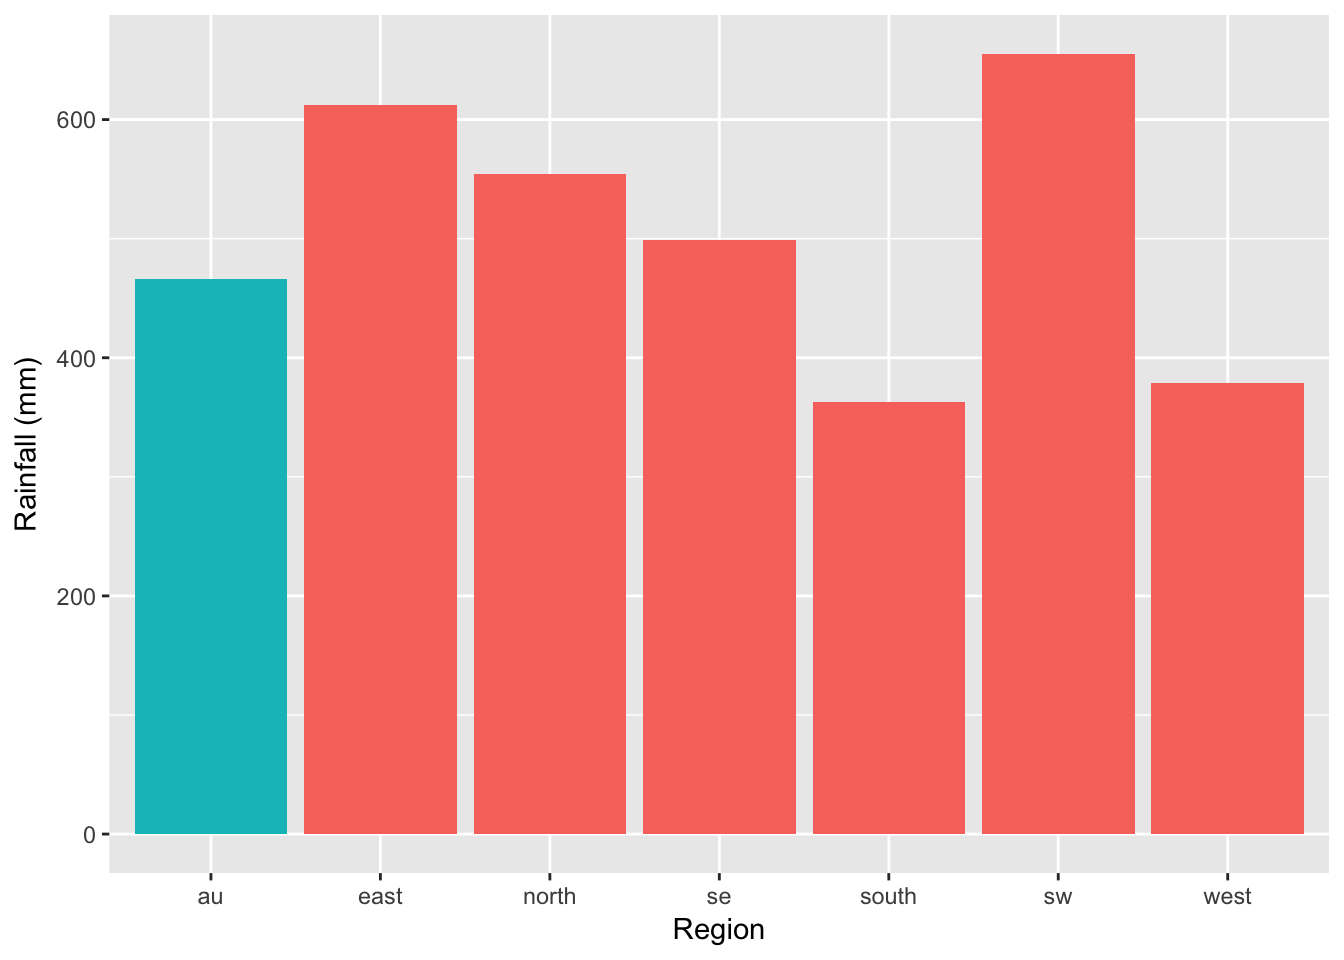
\includegraphics{graphics_files/figure-latex/unnamed-chunk-25-1.pdf}

If we weren't interested in the time series and just wanted to focus on the most
recent year, we might take a different approach. Here a bar plot is used to
compare between regions, with the national average (au) highlighted in blue:

\begin{Shaded}
\begin{Highlighting}[]
\NormalTok{rain }\OperatorTok
\StringTok{  }\KeywordTok{filter}\NormalTok{(Year }\OperatorTok{==}\StringTok{ }\KeywordTok{max}\NormalTok{(Year)) }\OperatorTok
\StringTok{  }\KeywordTok{ggplot}\NormalTok{(}\KeywordTok{aes}\NormalTok{(Region, value, }\DataTypeTok{fill=}\NormalTok{Region}\OperatorTok{==}\StringTok{"au"}\NormalTok{)) }\OperatorTok{+}
\StringTok{  }\KeywordTok{stat_summary}\NormalTok{(}\DataTypeTok{geom=}\StringTok{"bar"}\NormalTok{) }\OperatorTok{+}
\StringTok{  }\KeywordTok{ylab}\NormalTok{(}\StringTok{'Rainfall (mm)'}\NormalTok{) }\OperatorTok{+}
\StringTok{  }\KeywordTok{guides}\NormalTok{(}\DataTypeTok{fill=}\NormalTok{F)}
\end{Highlighting}
\end{Shaded}

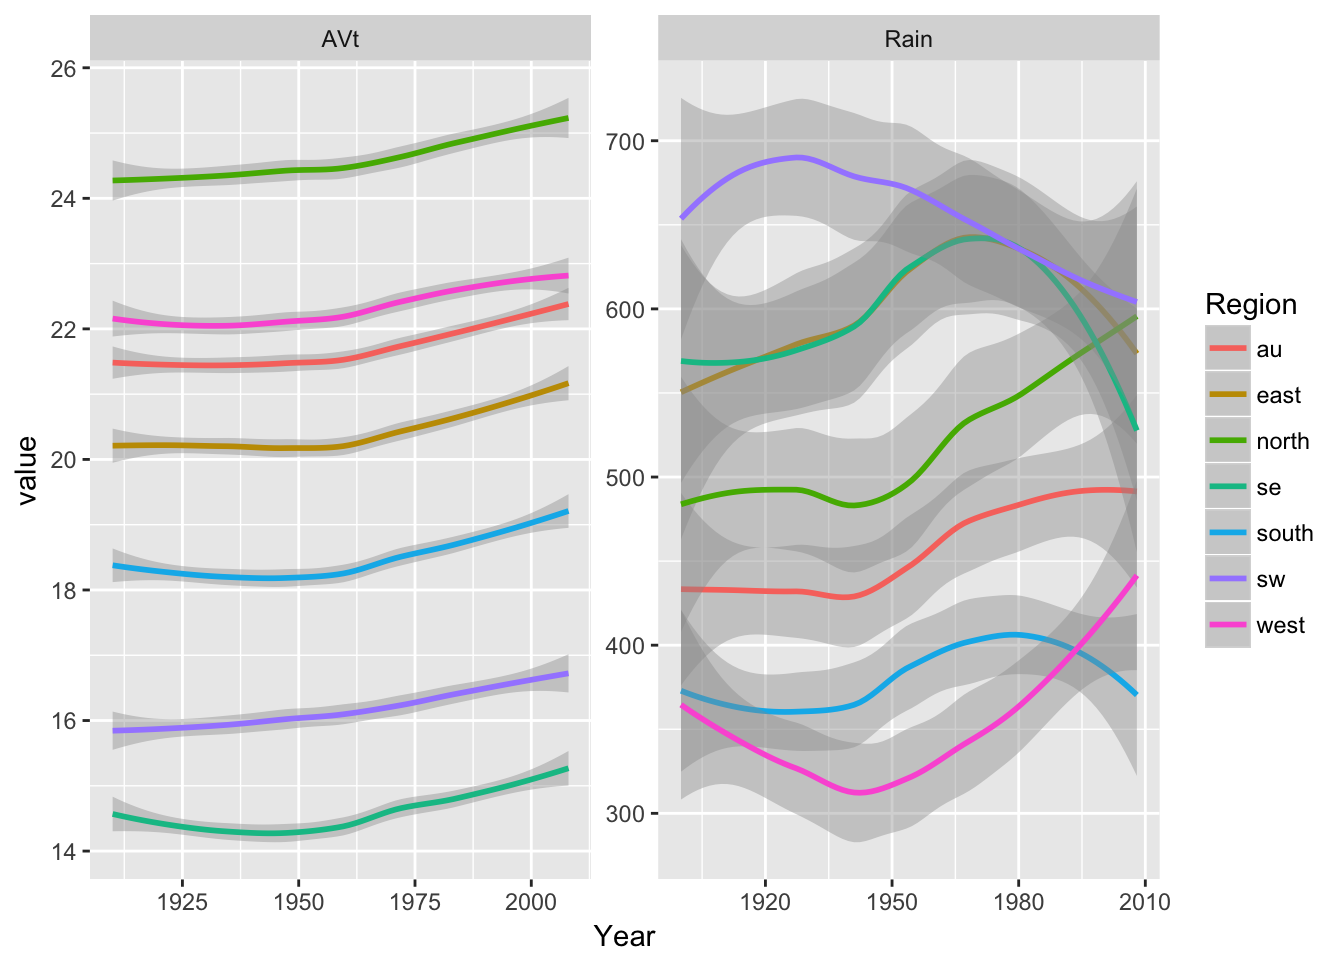
\includegraphics{graphics_files/figure-latex/unnamed-chunk-26-1.pdf}

Finally, we shouldn't forget that this dataset included both rainfall and
temperature data, and we can display these in different ways, depending on what
our research question was.

In this case we can use facetting to display temperature and rainfall data side
by side. Because AVt and Rain are on such different scales we need to allow the
y axis to vary between variables:

\begin{Shaded}
\begin{Highlighting}[]
\NormalTok{weather.data.long }\OperatorTok
\StringTok{  }\KeywordTok{ggplot}\NormalTok{(}\KeywordTok{aes}\NormalTok{(Year, value, }\DataTypeTok{color=}\NormalTok{Region)) }\OperatorTok{+}
\StringTok{  }\KeywordTok{geom_smooth}\NormalTok{() }\OperatorTok{+}
\StringTok{  }\KeywordTok{facet_wrap}\NormalTok{(}\OperatorTok{~}\NormalTok{variable, }\DataTypeTok{scales=}\StringTok{"free"}\NormalTok{)}
\NormalTok{Warning}\OperatorTok{:}\StringTok{ }\NormalTok{Removed }\DecValTok{70}\NormalTok{ rows containing non}\OperatorTok{-}\NormalTok{finite }\KeywordTok{values}\NormalTok{ (stat_smooth).}
\end{Highlighting}
\end{Shaded}

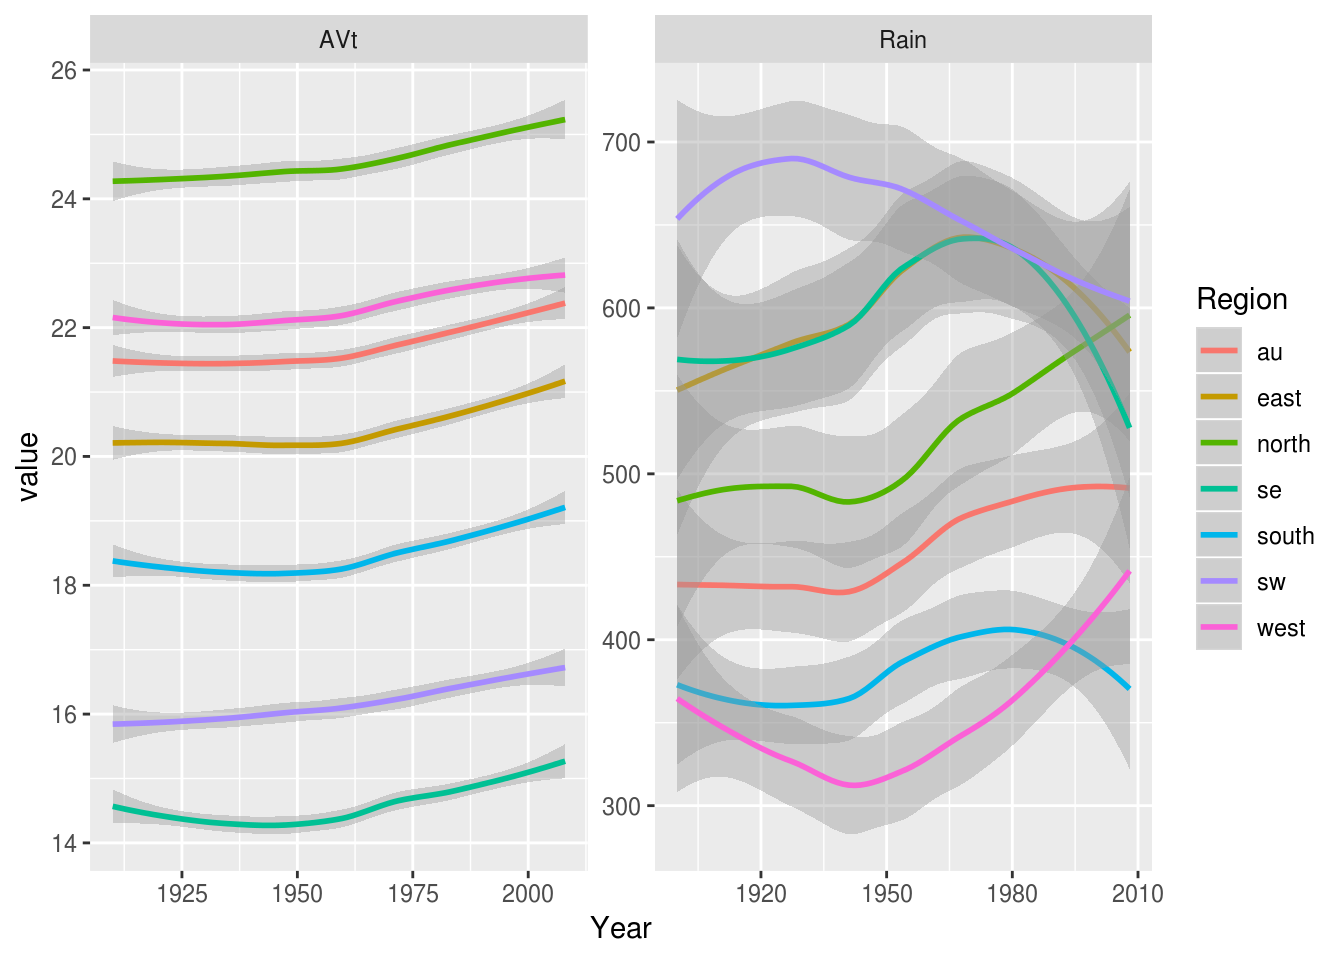
\includegraphics{graphics_files/figure-latex/unnamed-chunk-27-1.pdf}

\hypertarget{composition}{%
\subsubsection*{`Composition'}\label{composition}}
\addcontentsline{toc}{subsubsection}{`Composition'}

\hypertarget{waffle-plots-or-pictograms}{%
\paragraph{Waffle plots or `pictograms'}\label{waffle-plots-or-pictograms}}
\addcontentsline{toc}{paragraph}{Waffle plots or `pictograms'}

Waffle plots are neat way of showing the relative frequency of different
categories.

In applied settings it's well known that when considering the risks or benefits
of interventions clinicans, patients and researchers benefit from statements
made using `natural frequencies' \citep{gigerenzer2003simple}, and pictographs or
`waffle plots' have been shown to provide patients and their families with a
better understanding of the risks of treatments \citep{tait2010presenting}.

Waffle plots can be implemented in R via the \texttt{waffle::} package:

\begin{Shaded}
\begin{Highlighting}[]
\NormalTok{outcomes <-}\StringTok{ }\KeywordTok{c}\NormalTok{(}\StringTok{"gained weight"}\NormalTok{=}\DecValTok{13}\NormalTok{,}
              \StringTok{"no change"}\NormalTok{=}\DecValTok{27}\NormalTok{,}
              \StringTok{"lost 2kg or more"}\NormalTok{ =}\StringTok{ }\DecValTok{44}\NormalTok{,}
              \StringTok{"lost 5kg or more"}\NormalTok{ =}\StringTok{ }\DecValTok{16}\NormalTok{)}

\NormalTok{waffle}\OperatorTok{::}\KeywordTok{waffle}\NormalTok{(outcomes)}
\end{Highlighting}
\end{Shaded}

\includegraphics{graphics_files/figure-latex/unnamed-chunk-28-1.pdf}

{Calculating these summary figures is left as an exercise to for the reader, but
see the section on \protect\hyperlink{split-apply-combine}{summarising data with dplyr}.}

This is one of those occasions where the default ggplot colours could probably
be improved, and we can do this by passing the
\protect\hyperlink{named-colours}{names of the colours} we would like to use:

\begin{Shaded}
\begin{Highlighting}[]
\NormalTok{weight.loss.colours <-}\StringTok{ }\KeywordTok{c}\NormalTok{(}\StringTok{'firebrick2'}\NormalTok{, }\StringTok{'darkgoldenrod1'}\NormalTok{, }\StringTok{'palegreen3'}\NormalTok{, }\StringTok{'palegreen4'}\NormalTok{)}
\NormalTok{waffle}\OperatorTok{::}\KeywordTok{waffle}\NormalTok{(outcomes, }\DataTypeTok{colors =}\NormalTok{ weight.loss.colours)}
\end{Highlighting}
\end{Shaded}

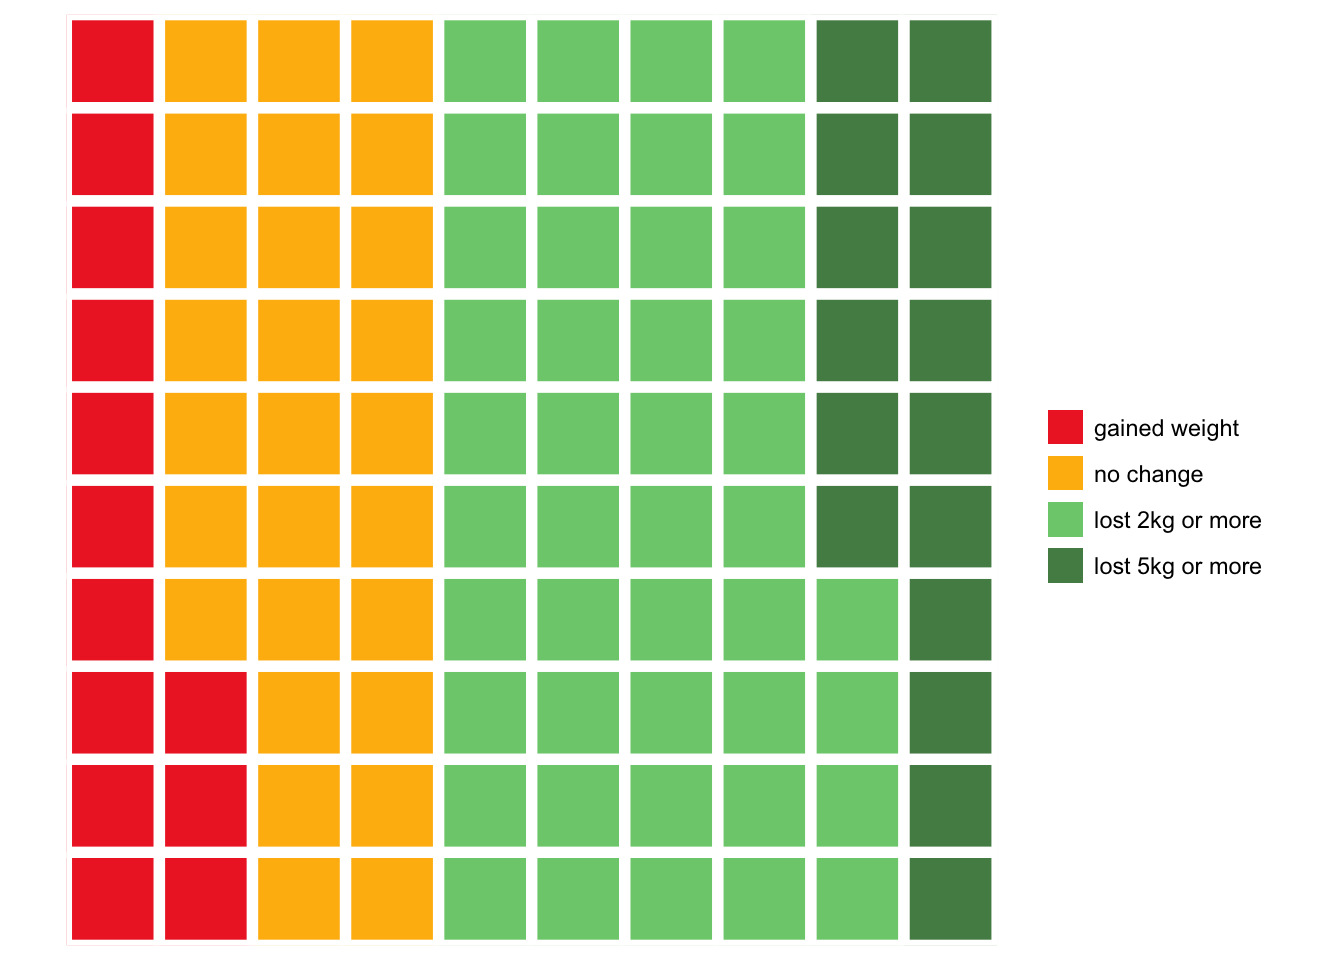
\includegraphics{graphics_files/figure-latex/unnamed-chunk-29-1.pdf}

Selecting colours by hand isn't always the best way though: the
\protect\hyperlink{color-brewer}{\texttt{colourbrewer} library provides some nice shortcuts} for using
palletes from the excellent \href{http://colorbrewer2.org}{ColourBrewer website}.

\hypertarget{stacked-bars}{%
\paragraph{Stacked bars}\label{stacked-bars}}
\addcontentsline{toc}{paragraph}{Stacked bars}

The \texttt{reshape2} package includes data on tipping habits in restaurants for male
and female bill-payers, and where the party was fo various \texttt{size}s:

\begin{Shaded}
\begin{Highlighting}[]
\NormalTok{reshape2}\OperatorTok{::}\NormalTok{tips }\OperatorTok
\StringTok{  }\NormalTok{head }\OperatorTok
\StringTok{  }\NormalTok{pander}
\end{Highlighting}
\end{Shaded}

\begin{longtable}[]{@{}ccccccc@{}}
\toprule
\begin{minipage}[b]{0.15\columnwidth}\centering
total\_bill\strut
\end{minipage} & \begin{minipage}[b]{0.08\columnwidth}\centering
tip\strut
\end{minipage} & \begin{minipage}[b]{0.10\columnwidth}\centering
sex\strut
\end{minipage} & \begin{minipage}[b]{0.10\columnwidth}\centering
smoker\strut
\end{minipage} & \begin{minipage}[b]{0.07\columnwidth}\centering
day\strut
\end{minipage} & \begin{minipage}[b]{0.10\columnwidth}\centering
time\strut
\end{minipage} & \begin{minipage}[b]{0.10\columnwidth}\centering
size\strut
\end{minipage}\tabularnewline
\midrule
\endhead
\begin{minipage}[t]{0.15\columnwidth}\centering
16.99\strut
\end{minipage} & \begin{minipage}[t]{0.08\columnwidth}\centering
1.01\strut
\end{minipage} & \begin{minipage}[t]{0.10\columnwidth}\centering
Female\strut
\end{minipage} & \begin{minipage}[t]{0.10\columnwidth}\centering
No\strut
\end{minipage} & \begin{minipage}[t]{0.07\columnwidth}\centering
Sun\strut
\end{minipage} & \begin{minipage}[t]{0.10\columnwidth}\centering
Dinner\strut
\end{minipage} & \begin{minipage}[t]{0.10\columnwidth}\centering
2\strut
\end{minipage}\tabularnewline
\begin{minipage}[t]{0.15\columnwidth}\centering
10.34\strut
\end{minipage} & \begin{minipage}[t]{0.08\columnwidth}\centering
1.66\strut
\end{minipage} & \begin{minipage}[t]{0.10\columnwidth}\centering
Male\strut
\end{minipage} & \begin{minipage}[t]{0.10\columnwidth}\centering
No\strut
\end{minipage} & \begin{minipage}[t]{0.07\columnwidth}\centering
Sun\strut
\end{minipage} & \begin{minipage}[t]{0.10\columnwidth}\centering
Dinner\strut
\end{minipage} & \begin{minipage}[t]{0.10\columnwidth}\centering
3\strut
\end{minipage}\tabularnewline
\begin{minipage}[t]{0.15\columnwidth}\centering
21.01\strut
\end{minipage} & \begin{minipage}[t]{0.08\columnwidth}\centering
3.5\strut
\end{minipage} & \begin{minipage}[t]{0.10\columnwidth}\centering
Male\strut
\end{minipage} & \begin{minipage}[t]{0.10\columnwidth}\centering
No\strut
\end{minipage} & \begin{minipage}[t]{0.07\columnwidth}\centering
Sun\strut
\end{minipage} & \begin{minipage}[t]{0.10\columnwidth}\centering
Dinner\strut
\end{minipage} & \begin{minipage}[t]{0.10\columnwidth}\centering
3\strut
\end{minipage}\tabularnewline
\begin{minipage}[t]{0.15\columnwidth}\centering
23.68\strut
\end{minipage} & \begin{minipage}[t]{0.08\columnwidth}\centering
3.31\strut
\end{minipage} & \begin{minipage}[t]{0.10\columnwidth}\centering
Male\strut
\end{minipage} & \begin{minipage}[t]{0.10\columnwidth}\centering
No\strut
\end{minipage} & \begin{minipage}[t]{0.07\columnwidth}\centering
Sun\strut
\end{minipage} & \begin{minipage}[t]{0.10\columnwidth}\centering
Dinner\strut
\end{minipage} & \begin{minipage}[t]{0.10\columnwidth}\centering
2\strut
\end{minipage}\tabularnewline
\begin{minipage}[t]{0.15\columnwidth}\centering
24.59\strut
\end{minipage} & \begin{minipage}[t]{0.08\columnwidth}\centering
3.61\strut
\end{minipage} & \begin{minipage}[t]{0.10\columnwidth}\centering
Female\strut
\end{minipage} & \begin{minipage}[t]{0.10\columnwidth}\centering
No\strut
\end{minipage} & \begin{minipage}[t]{0.07\columnwidth}\centering
Sun\strut
\end{minipage} & \begin{minipage}[t]{0.10\columnwidth}\centering
Dinner\strut
\end{minipage} & \begin{minipage}[t]{0.10\columnwidth}\centering
4\strut
\end{minipage}\tabularnewline
\begin{minipage}[t]{0.15\columnwidth}\centering
25.29\strut
\end{minipage} & \begin{minipage}[t]{0.08\columnwidth}\centering
4.71\strut
\end{minipage} & \begin{minipage}[t]{0.10\columnwidth}\centering
Male\strut
\end{minipage} & \begin{minipage}[t]{0.10\columnwidth}\centering
No\strut
\end{minipage} & \begin{minipage}[t]{0.07\columnwidth}\centering
Sun\strut
\end{minipage} & \begin{minipage}[t]{0.10\columnwidth}\centering
Dinner\strut
\end{minipage} & \begin{minipage}[t]{0.10\columnwidth}\centering
4\strut
\end{minipage}\tabularnewline
\bottomrule
\end{longtable}

To begin, we might like to plot tips by time of day:

\begin{Shaded}
\begin{Highlighting}[]
\NormalTok{reshape2}\OperatorTok{::}\NormalTok{tips }\OperatorTok
\StringTok{  }\KeywordTok{ggplot}\NormalTok{(}\KeywordTok{aes}\NormalTok{(time, tip)) }\OperatorTok{+}
\StringTok{  }\KeywordTok{stat_summary}\NormalTok{(}\DataTypeTok{geom=}\StringTok{"bar"}\NormalTok{)}
\end{Highlighting}
\end{Shaded}

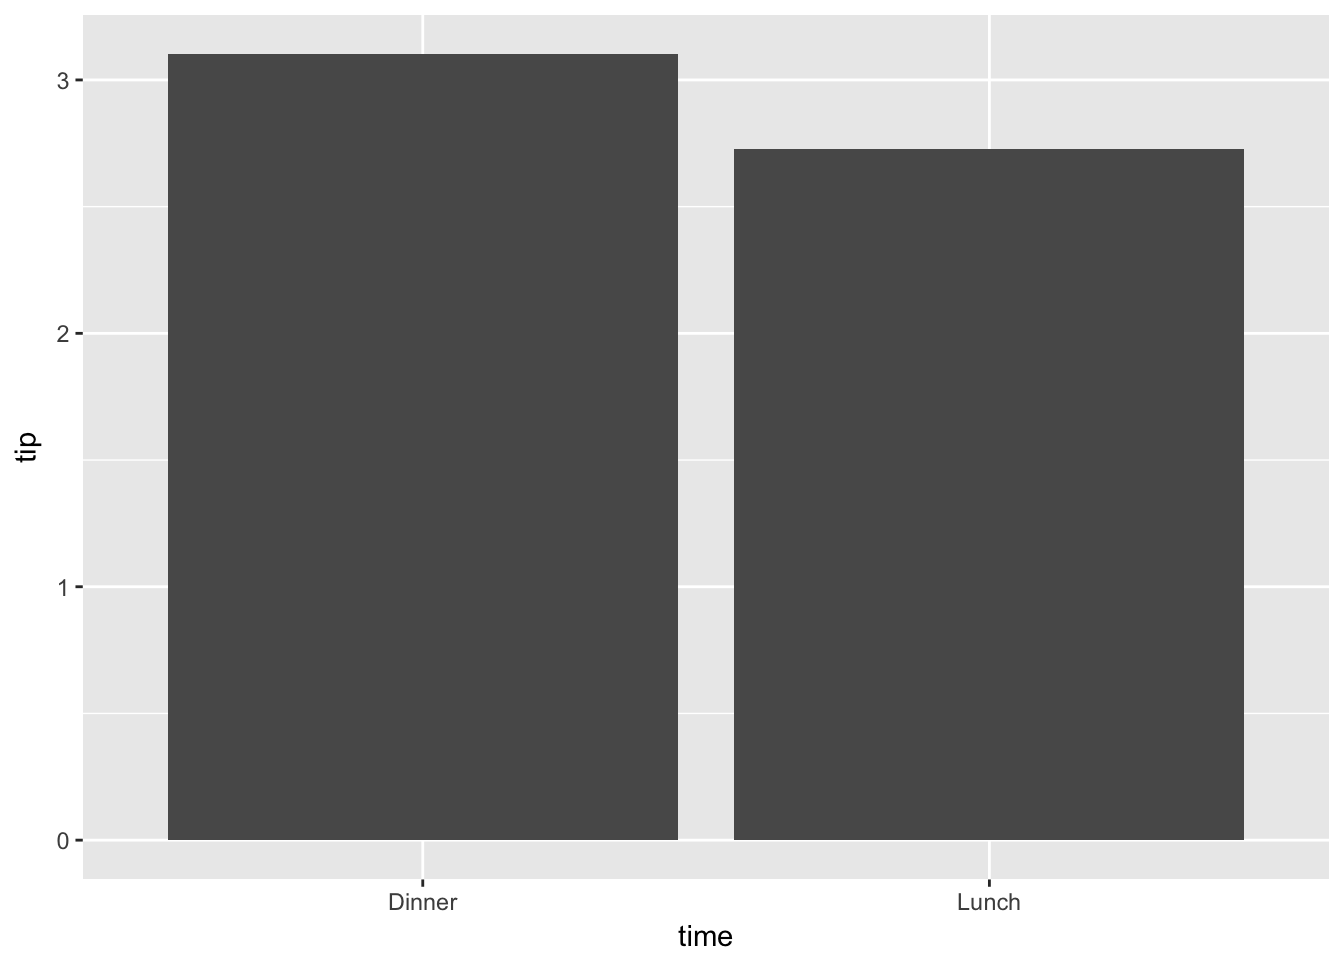
\includegraphics{graphics_files/figure-latex/unnamed-chunk-31-1.pdf}

And to facilitate the comparison between men and women we could colour portions
of the bars using \texttt{position\_stack()}:

\begin{Shaded}
\begin{Highlighting}[]
\NormalTok{reshape2}\OperatorTok{::}\NormalTok{tips }\OperatorTok
\StringTok{  }\KeywordTok{ggplot}\NormalTok{(}\KeywordTok{aes}\NormalTok{(time, tip, }\DataTypeTok{fill=}\NormalTok{sex)) }\OperatorTok{+}
\StringTok{  }\KeywordTok{stat_summary}\NormalTok{(}\DataTypeTok{geom=}\StringTok{"bar"}\NormalTok{, }\DataTypeTok{position=}\KeywordTok{position_stack}\NormalTok{()) }\OperatorTok{+}
\StringTok{  }\KeywordTok{xlab}\NormalTok{(}\StringTok{""}\NormalTok{) }\OperatorTok{+}\StringTok{ }\KeywordTok{ylab}\NormalTok{(}\StringTok{"Tip ($)"}\NormalTok{)}
\end{Highlighting}
\end{Shaded}

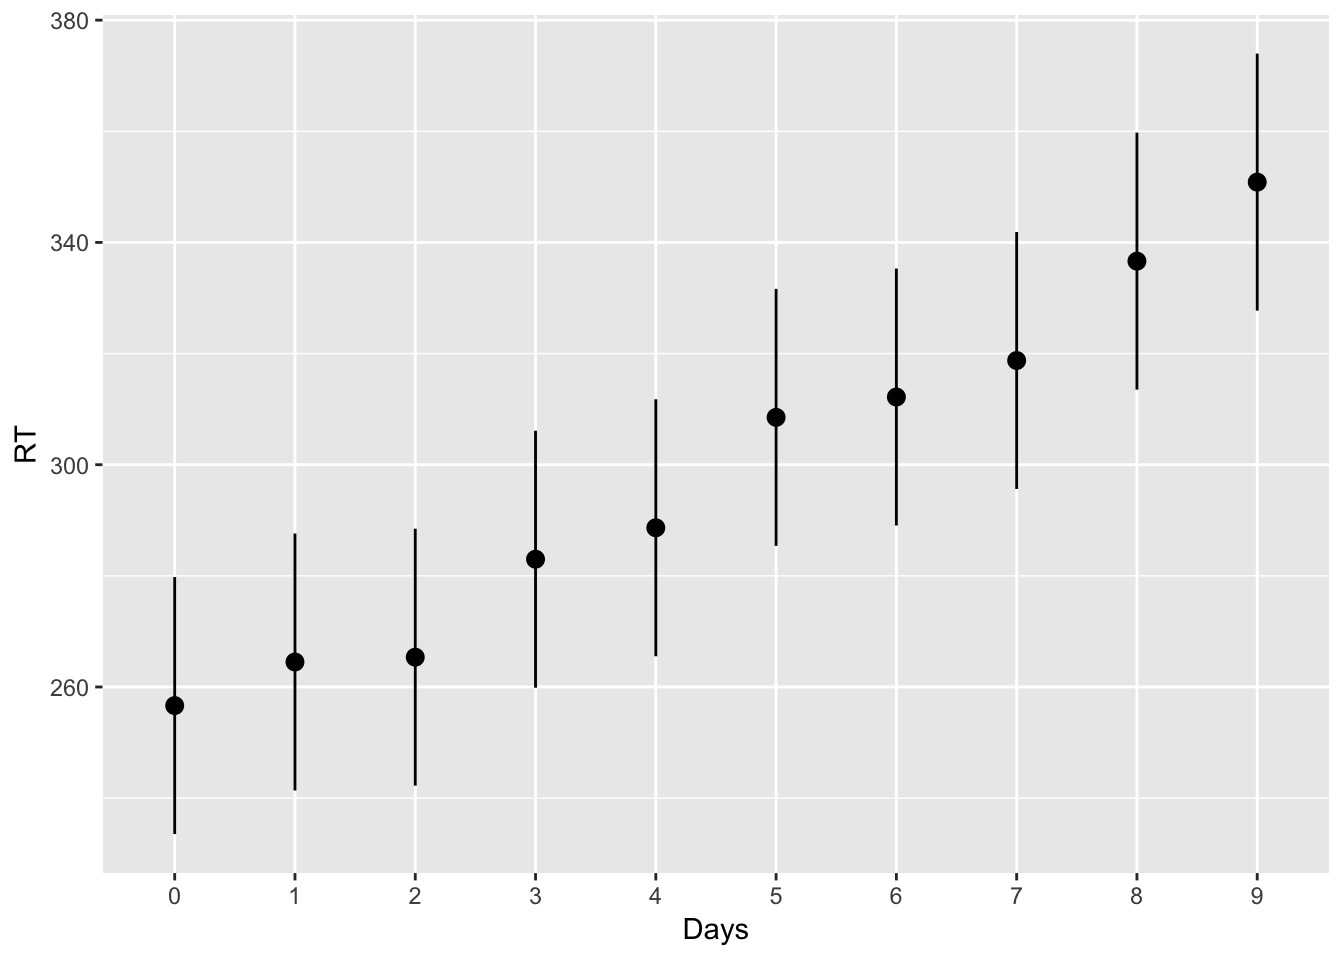
\includegraphics{graphics_files/figure-latex/unnamed-chunk-32-1.pdf}

Or to reverse the comparisons:

\begin{Shaded}
\begin{Highlighting}[]
\NormalTok{reshape2}\OperatorTok{::}\NormalTok{tips }\OperatorTok
\StringTok{  }\KeywordTok{ggplot}\NormalTok{(}\KeywordTok{aes}\NormalTok{(sex, tip, }\DataTypeTok{fill=}\NormalTok{time)) }\OperatorTok{+}
\StringTok{  }\KeywordTok{stat_summary}\NormalTok{(}\DataTypeTok{geom=}\StringTok{"bar"}\NormalTok{, }\DataTypeTok{position=}\KeywordTok{position_stack}\NormalTok{()) }\OperatorTok{+}
\StringTok{  }\KeywordTok{xlab}\NormalTok{(}\StringTok{""}\NormalTok{) }\OperatorTok{+}\StringTok{ }\KeywordTok{ylab}\NormalTok{(}\StringTok{"Tip ($)"}\NormalTok{)}
\end{Highlighting}
\end{Shaded}

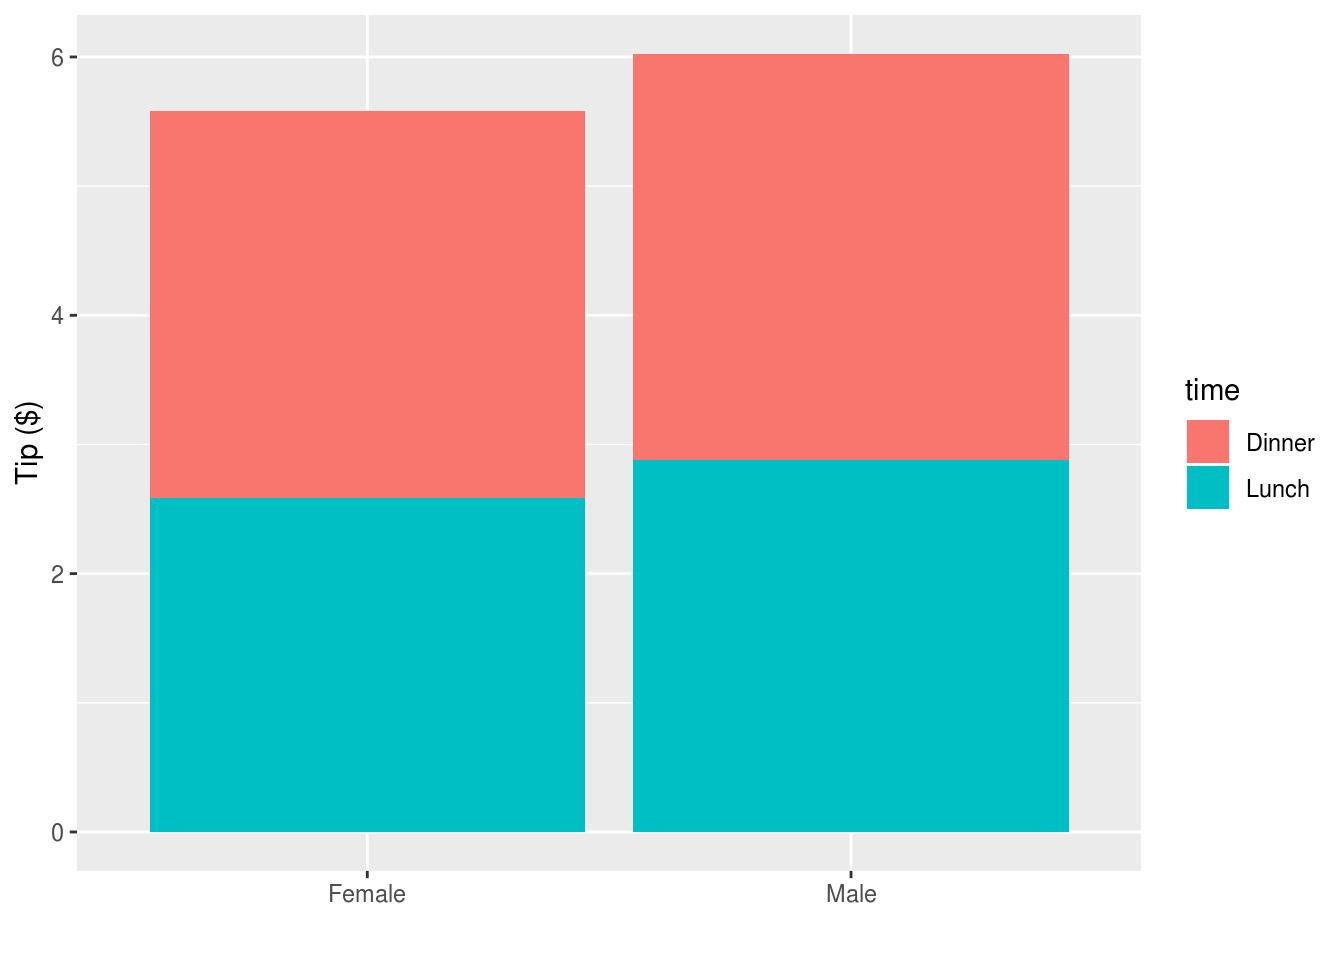
\includegraphics{graphics_files/figure-latex/unnamed-chunk-33-1.pdf}

\hypertarget{utility-plotting-functions}{%
\subsection*{`Quick and dirty' (utility) plots}\label{utility-plotting-functions}}
\addcontentsline{toc}{subsection}{`Quick and dirty' (utility) plots}

When exploring a dataset, often useful to use built in functions or helpers from
other libraries. These help you quickly visualise relationships, but aren't
always \emph{exactly} what you need and can be hard to customise.

\hypertarget{distributions-1}{%
\subsubsection{Distributions}\label{distributions-1}}

\begin{Shaded}
\begin{Highlighting}[]
\KeywordTok{hist}\NormalTok{(mtcars}\OperatorTok{$}\NormalTok{mpg)}
\end{Highlighting}
\end{Shaded}

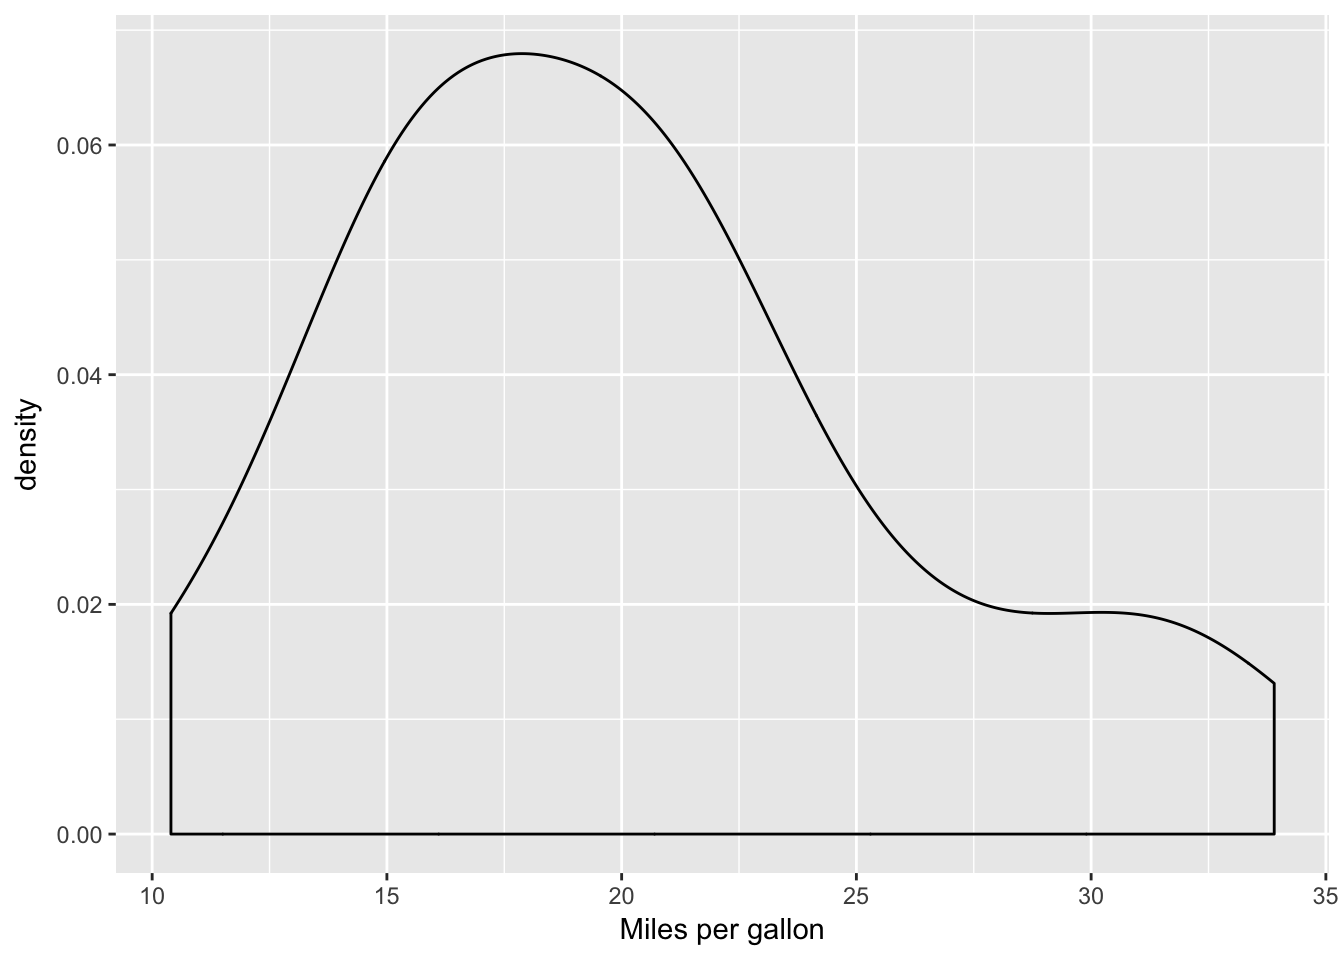
\includegraphics{graphics_files/figure-latex/unnamed-chunk-34-1.pdf}

\begin{Shaded}
\begin{Highlighting}[]
\KeywordTok{plot}\NormalTok{(}\KeywordTok{density}\NormalTok{(mtcars}\OperatorTok{$}\NormalTok{mpg))}
\end{Highlighting}
\end{Shaded}

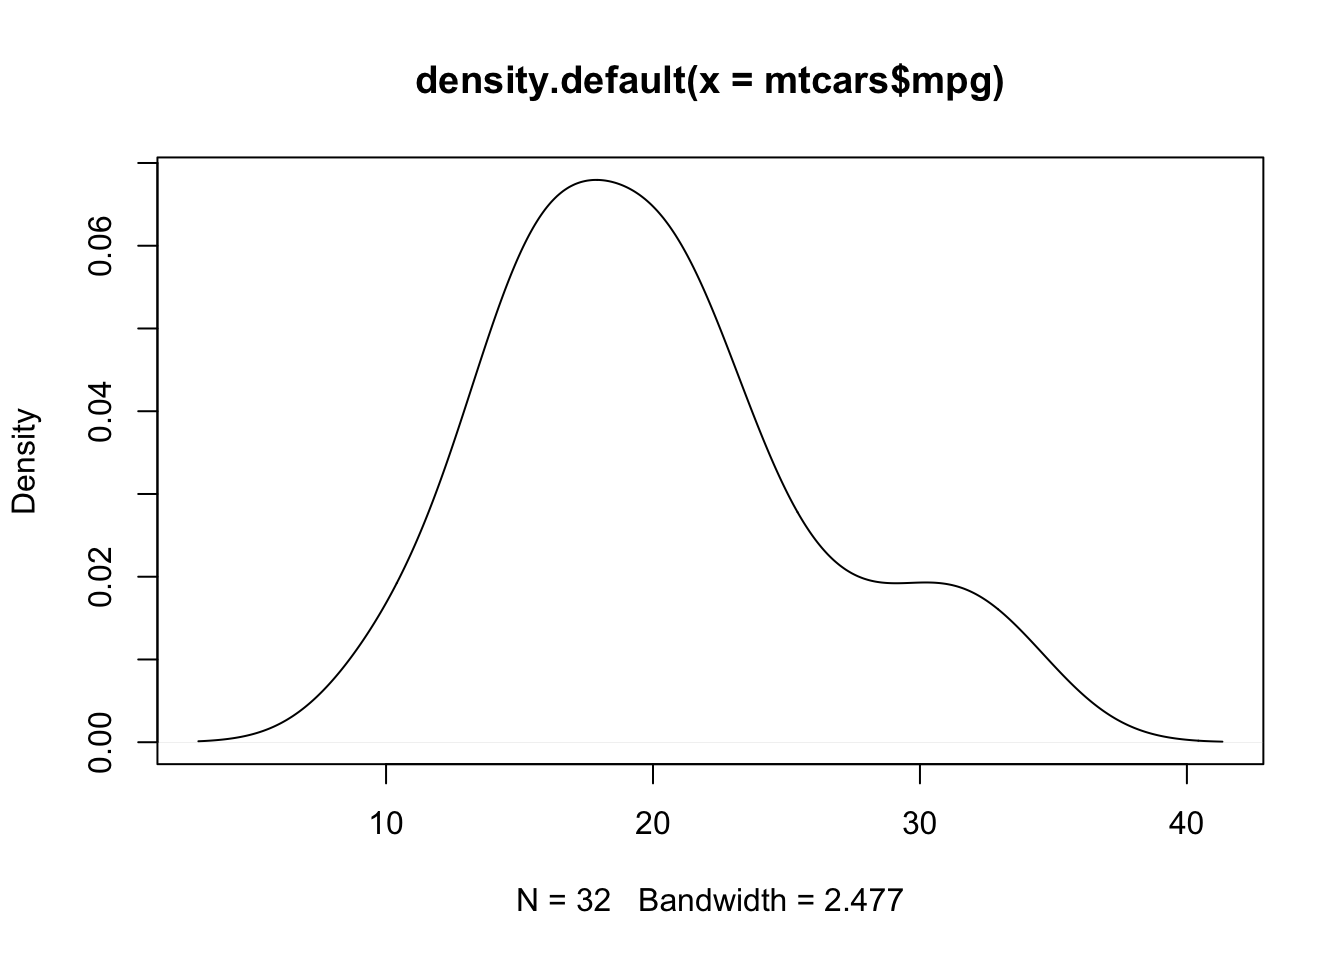
\includegraphics{graphics_files/figure-latex/unnamed-chunk-34-2.pdf}

\begin{Shaded}
\begin{Highlighting}[]
\KeywordTok{boxplot}\NormalTok{(mpg}\OperatorTok{~}\NormalTok{cyl, }\DataTypeTok{data=}\NormalTok{mtcars)}
\end{Highlighting}
\end{Shaded}

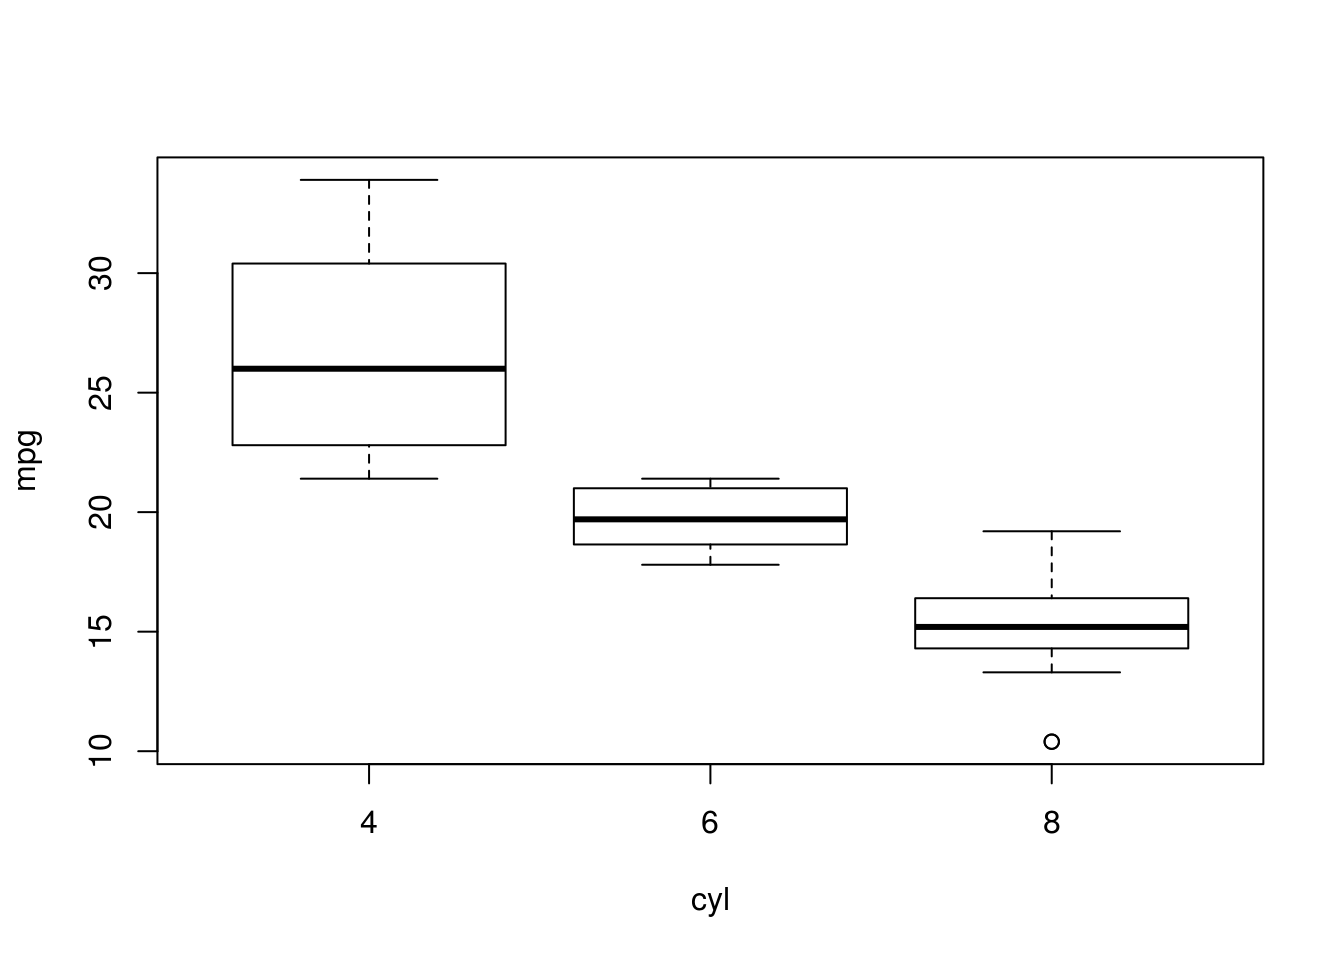
\includegraphics{graphics_files/figure-latex/unnamed-chunk-34-3.pdf}

\begin{Shaded}
\begin{Highlighting}[]
\NormalTok{Hmisc}\OperatorTok{::}\KeywordTok{hist.data.frame}\NormalTok{(mtcars)}
\end{Highlighting}
\end{Shaded}

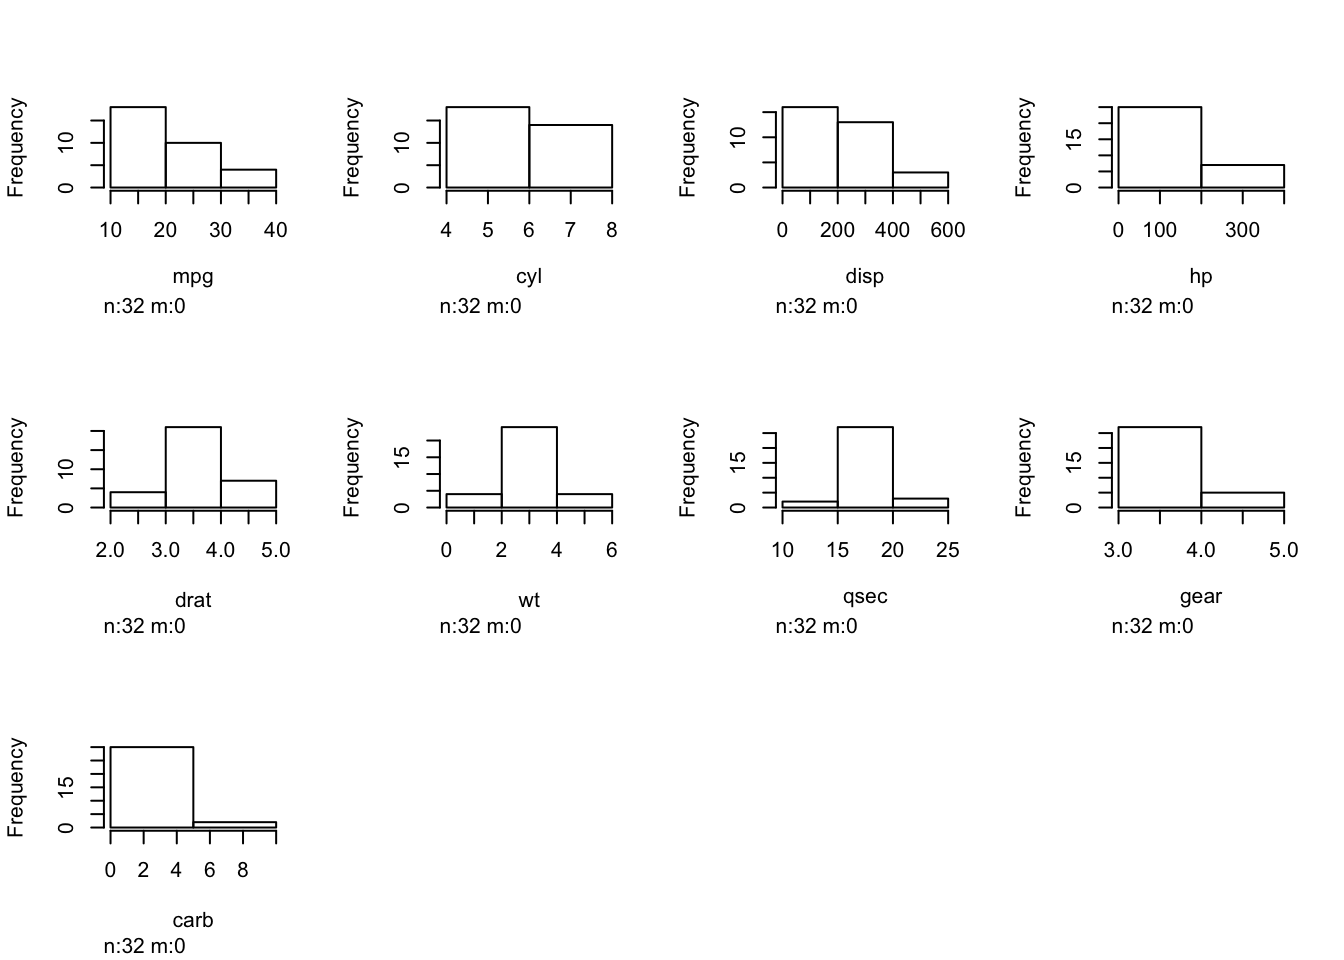
\includegraphics{graphics_files/figure-latex/unnamed-chunk-34-4.pdf}

Even for simple plots, ggplot has some useful helper functions though:

\begin{Shaded}
\begin{Highlighting}[]
\KeywordTok{qplot}\NormalTok{(mpg, }\DataTypeTok{data=}\NormalTok{mtcars, }\DataTypeTok{geom=}\StringTok{"density"}\NormalTok{) }\OperatorTok{+}\StringTok{ }\KeywordTok{xlab}\NormalTok{(}\StringTok{"Miles per gallon"}\NormalTok{)}
\end{Highlighting}
\end{Shaded}

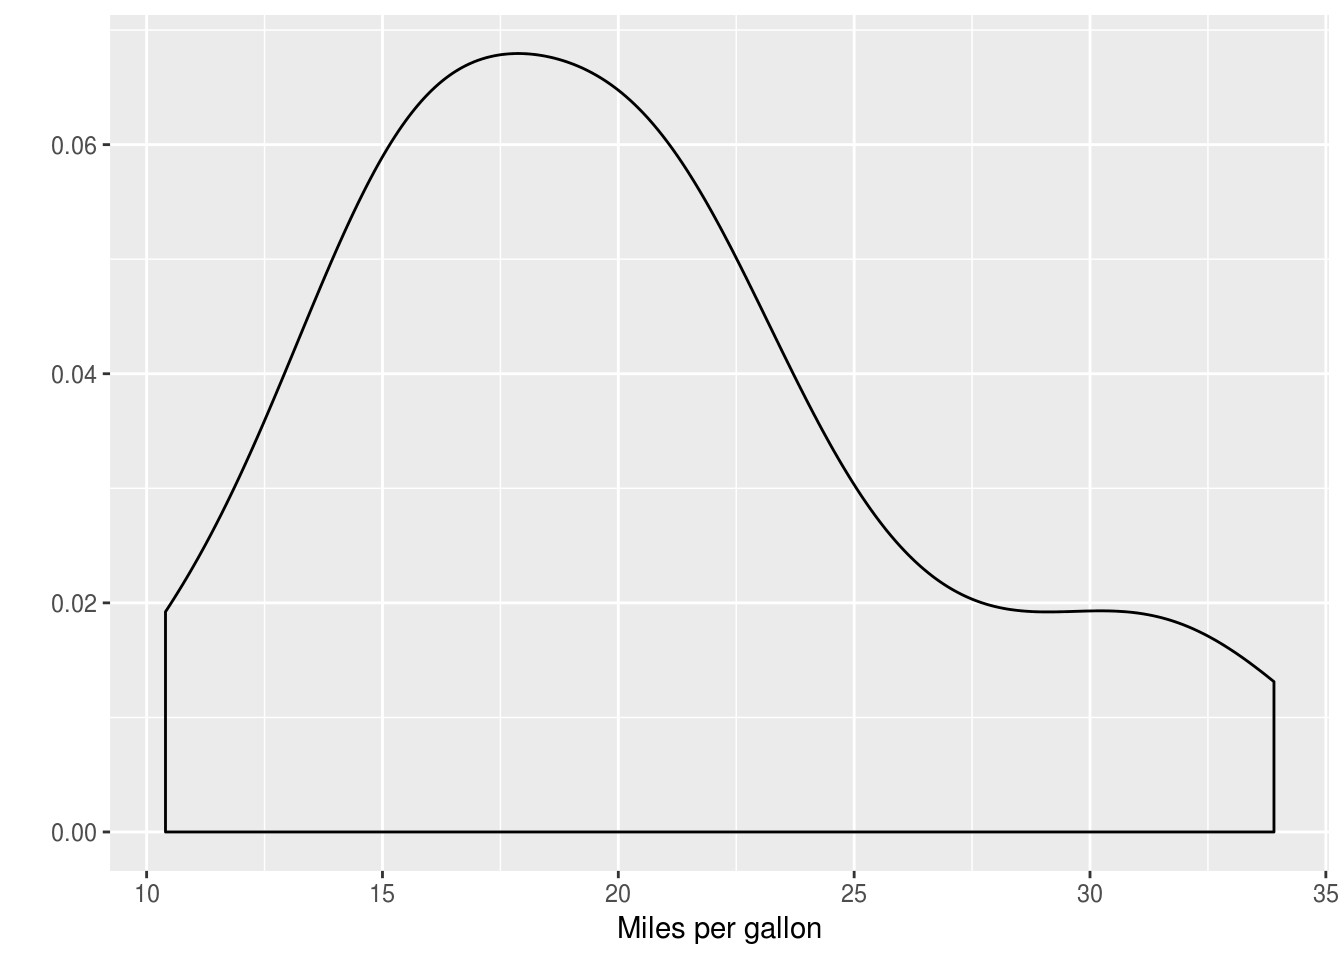
\includegraphics{graphics_files/figure-latex/unnamed-chunk-35-1.pdf}

\begin{Shaded}
\begin{Highlighting}[]
\KeywordTok{qplot}\NormalTok{(}\DataTypeTok{x=}\KeywordTok{factor}\NormalTok{(cyl), }\DataTypeTok{y=}\NormalTok{mpg, }\DataTypeTok{data=}\NormalTok{mtcars, }\DataTypeTok{geom=}\StringTok{"boxplot"}\NormalTok{)}
\end{Highlighting}
\end{Shaded}

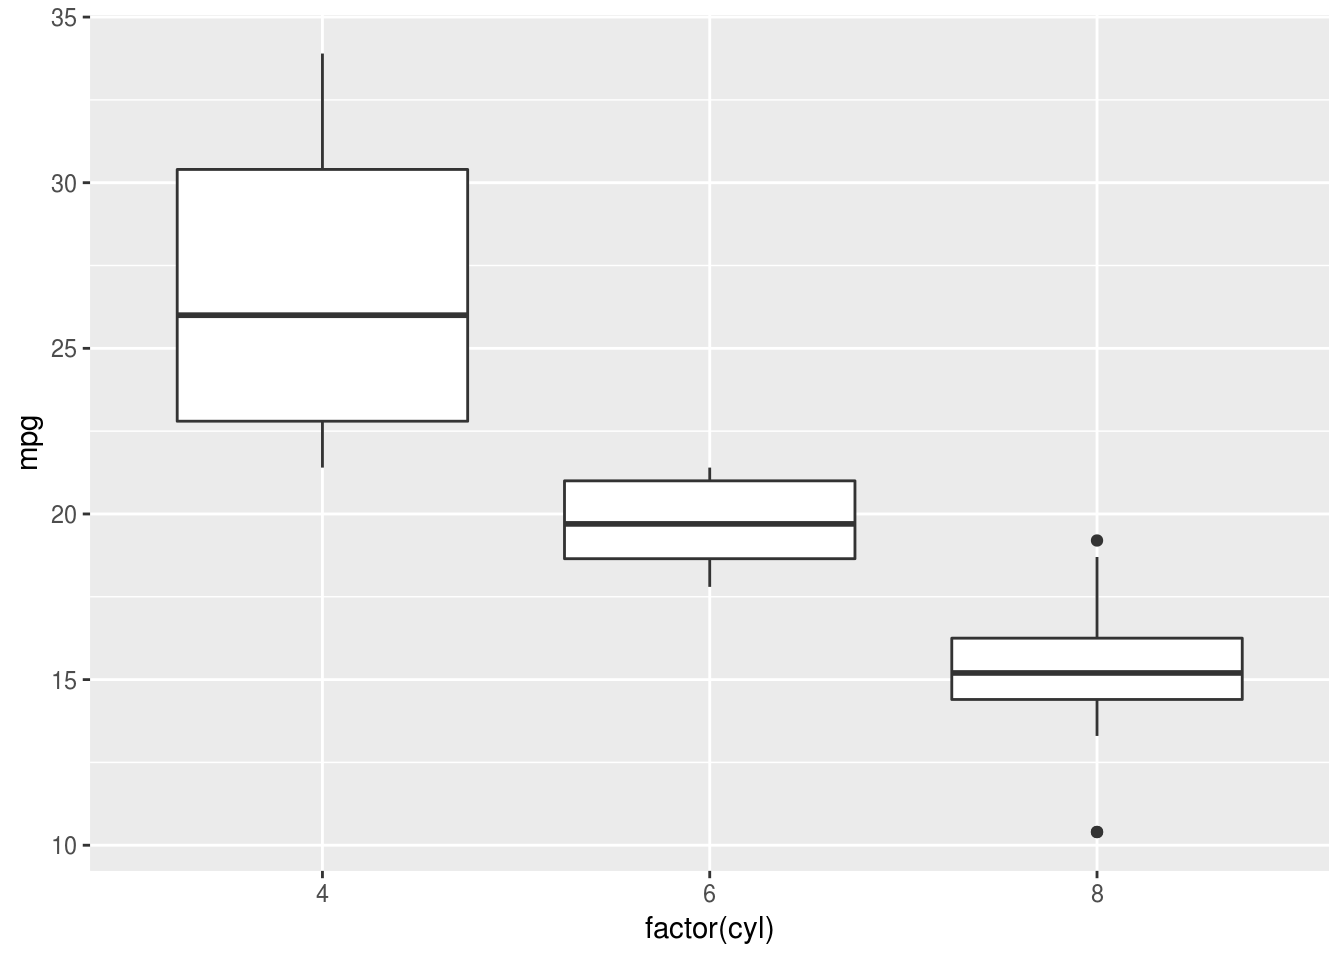
\includegraphics{graphics_files/figure-latex/unnamed-chunk-35-2.pdf}

\hypertarget{relationships-1}{%
\subsubsection{Relationships}\label{relationships-1}}

\begin{Shaded}
\begin{Highlighting}[]
\KeywordTok{with}\NormalTok{(mtcars, }\KeywordTok{plot}\NormalTok{(mpg, wt))}
\end{Highlighting}
\end{Shaded}

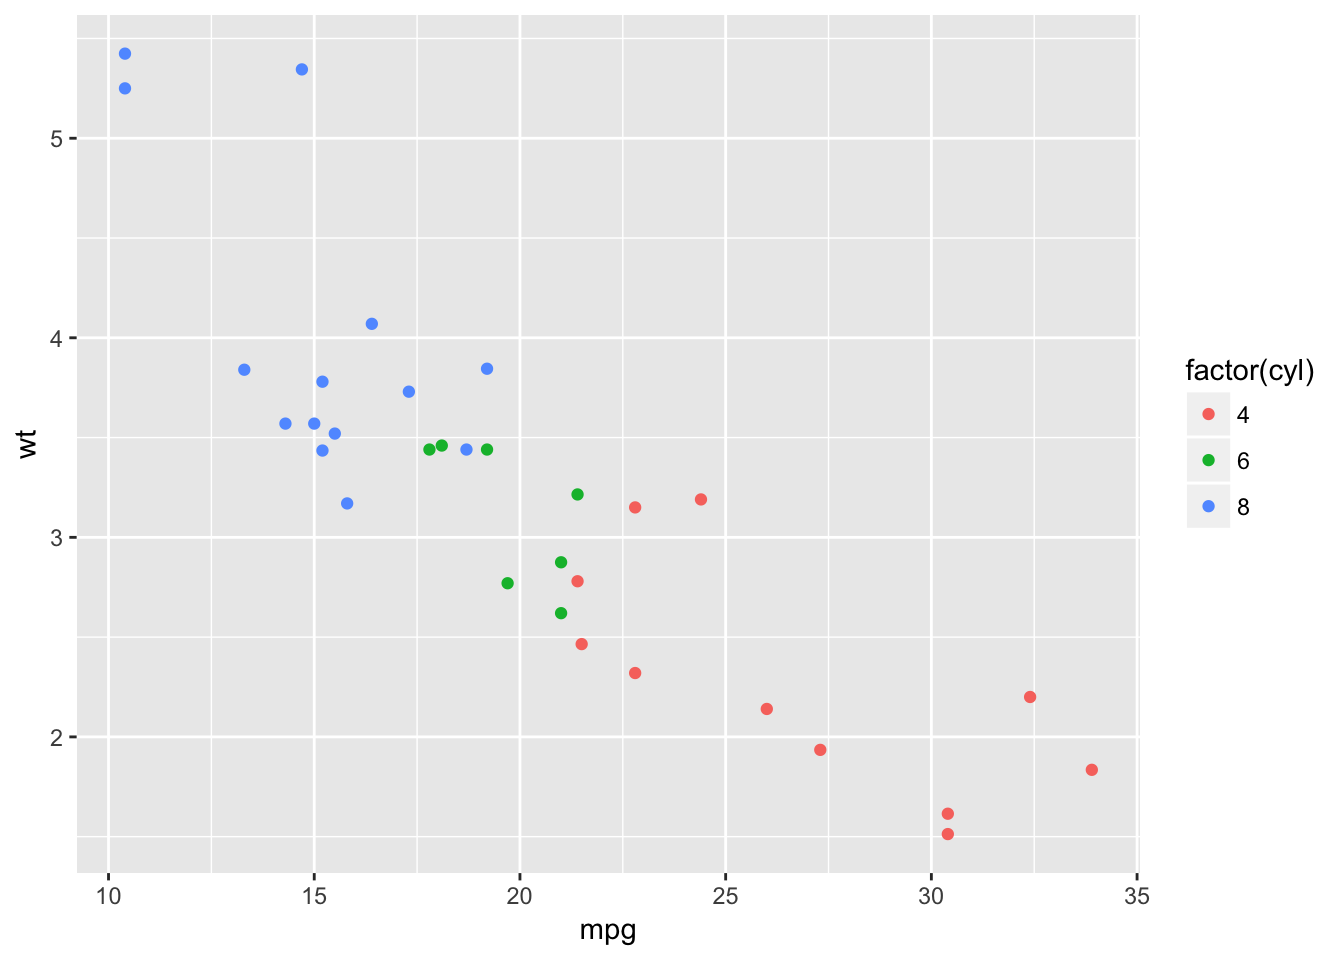
\includegraphics{graphics_files/figure-latex/unnamed-chunk-36-1.pdf}

\begin{Shaded}
\begin{Highlighting}[]
\KeywordTok{pairs}\NormalTok{(}\KeywordTok{select}\NormalTok{(mtcars, wt, disp, mpg))}
\end{Highlighting}
\end{Shaded}

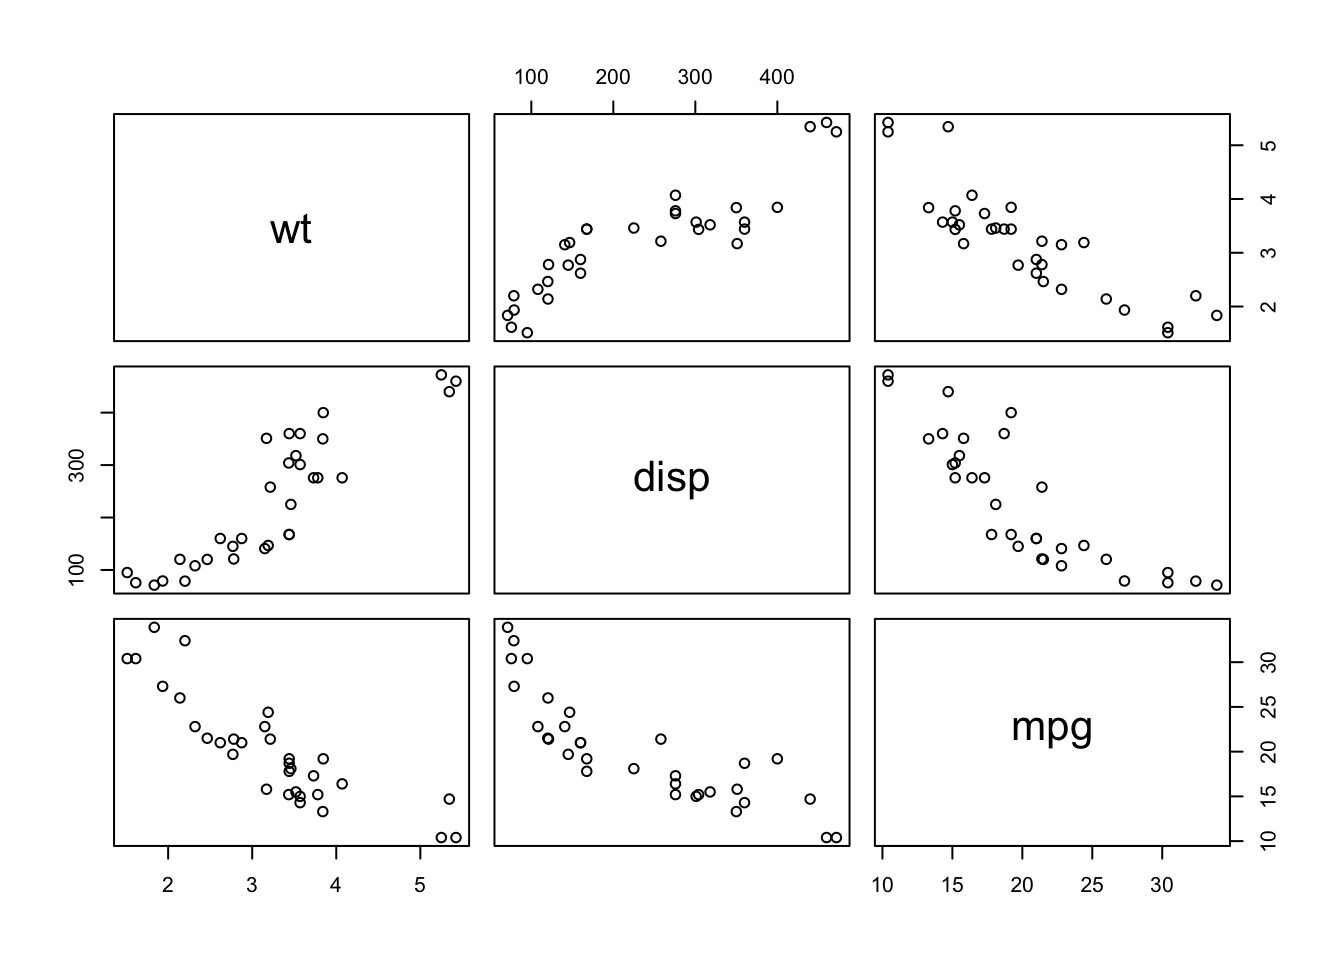
\includegraphics{graphics_files/figure-latex/unnamed-chunk-36-2.pdf}

Again, for quick plots ggplot also has useful shortcut functions:

\begin{Shaded}
\begin{Highlighting}[]
\KeywordTok{qplot}\NormalTok{(mpg, wt, }\DataTypeTok{color=}\KeywordTok{factor}\NormalTok{(cyl), }\DataTypeTok{data =}\NormalTok{ mtcars)}
\end{Highlighting}
\end{Shaded}

\includegraphics{graphics_files/figure-latex/unnamed-chunk-37-1.pdf}

\hypertarget{quantities}{%
\subsubsection{Quantities}\label{quantities}}

I don't think the base R plots are that convenient here. \texttt{ggplot2::} and the
\texttt{stat\_summary()} function makes life much simpler:

\begin{Shaded}
\begin{Highlighting}[]
\KeywordTok{ggplot}\NormalTok{(mtcars, }\KeywordTok{aes}\NormalTok{(}\KeywordTok{factor}\NormalTok{(cyl), mpg)) }\OperatorTok{+}
\StringTok{  }\KeywordTok{stat_summary}\NormalTok{(}\DataTypeTok{geom=}\StringTok{"bar"}\NormalTok{)}
\end{Highlighting}
\end{Shaded}

\includegraphics{graphics_files/figure-latex/unnamed-chunk-38-1.pdf}

And if you are plotting quantities, as disussed above, showing a range is
sensible (a boxplot would also fill both definitions):

\begin{Shaded}
\begin{Highlighting}[]
\KeywordTok{ggplot}\NormalTok{(mtcars, }\KeywordTok{aes}\NormalTok{(}\KeywordTok{factor}\NormalTok{(cyl), mpg)) }\OperatorTok{+}
\StringTok{  }\KeywordTok{stat_summary}\NormalTok{(}\DataTypeTok{geom=}\StringTok{"pointrange"}\NormalTok{)}
\end{Highlighting}
\end{Shaded}

\includegraphics{graphics_files/figure-latex/unnamed-chunk-39-1.pdf}

\hypertarget{ggplot-details}{%
\subsection*{Tricks with ggplot}\label{ggplot-details}}
\addcontentsline{toc}{subsection}{Tricks with ggplot}

\hypertarget{facetting-plots}{%
\subsubsection*{More ways to facet a plot}\label{facetting-plots}}
\addcontentsline{toc}{subsubsection}{More ways to facet a plot}

Facets are ways to repeat a plot for each level of another variable. \texttt{ggplot}
has two ways of defining and displaying facets:

\begin{itemize}
\tightlist
\item
  As a list of plots, using \texttt{facet\_wrap}.
\item
  As a grid or matrix of plots, using \texttt{facet\_grid()}.
\end{itemize}

Examples of both are shown below, using the following plot as a starting point:

\begin{Shaded}
\begin{Highlighting}[]
\NormalTok{base.plot <-}\StringTok{ }\KeywordTok{ggplot}\NormalTok{(mtcars, }\KeywordTok{aes}\NormalTok{(mpg, wt)) }\OperatorTok{+}\StringTok{ }\KeywordTok{geom_point}\NormalTok{()}
\NormalTok{base.plot}
\end{Highlighting}
\end{Shaded}

\includegraphics{graphics-ggplot-extras_files/figure-latex/unnamed-chunk-3-1.pdf}

\hypertarget{facet_wrap}{%
\subsubsection*{\texorpdfstring{\texttt{facet\_wrap}}{facet\_wrap}}\label{facet_wrap}}
\addcontentsline{toc}{subsubsection}{\texttt{facet\_wrap}}

If we want one facet we just type the tilde (\texttt{\textasciitilde{}}) symbol and then the name of
the variable. This is like typing the right hand side of a
\href{formulae}{formula for a regression model}:

\begin{Shaded}
\begin{Highlighting}[]
\NormalTok{base.plot }\OperatorTok{+}\StringTok{ }\KeywordTok{facet_wrap}\NormalTok{(}\OperatorTok{~}\NormalTok{cyl)}
\end{Highlighting}
\end{Shaded}

\includegraphics{graphics-ggplot-extras_files/figure-latex/unnamed-chunk-4-1.pdf}

If we want two facets we extend the formula, using the \texttt{+} sign:

\begin{Shaded}
\begin{Highlighting}[]
\NormalTok{base.plot }\OperatorTok{+}\StringTok{ }\KeywordTok{facet_wrap}\NormalTok{(}\OperatorTok{~}\NormalTok{cyl}\OperatorTok{+}\NormalTok{am)}
\end{Highlighting}
\end{Shaded}

\includegraphics{graphics-ggplot-extras_files/figure-latex/unnamed-chunk-5-1.pdf}

Note, the order of variables in the formula makes a difference:

\begin{Shaded}
\begin{Highlighting}[]
\NormalTok{base.plot }\OperatorTok{+}\StringTok{ }\KeywordTok{facet_wrap}\NormalTok{(}\OperatorTok{~}\NormalTok{am}\OperatorTok{+}\NormalTok{cyl)}
\end{Highlighting}
\end{Shaded}

\includegraphics{graphics-ggplot-extras_files/figure-latex/unnamed-chunk-6-1.pdf}

\hypertarget{facet_grid}{%
\subsubsection*{\texorpdfstring{\texttt{facet\_grid}}{facet\_grid}}\label{facet_grid}}
\addcontentsline{toc}{subsubsection}{\texttt{facet\_grid}}

With one variable \texttt{facet\_grid} produces similar output. Note the \texttt{.} (period) on
the left hand side of the formula now to make explicit we only have one
variable, and we want it on the x axis:

\begin{Shaded}
\begin{Highlighting}[]
\NormalTok{base.plot }\OperatorTok{+}\StringTok{ }\KeywordTok{facet_grid}\NormalTok{(.}\OperatorTok{~}\NormalTok{cyl)}
\end{Highlighting}
\end{Shaded}

\includegraphics{graphics-ggplot-extras_files/figure-latex/unnamed-chunk-7-1.pdf}

We can flip the facets around by putting the \texttt{cyl} variable on the left hand
side of the \texttt{\textasciitilde{}}:

\begin{Shaded}
\begin{Highlighting}[]
\NormalTok{base.plot }\OperatorTok{+}\StringTok{ }\KeywordTok{facet_grid}\NormalTok{(cyl}\OperatorTok{~}\NormalTok{.)}
\end{Highlighting}
\end{Shaded}

\includegraphics{graphics-ggplot-extras_files/figure-latex/unnamed-chunk-8-1.pdf}

And \texttt{facet\_grid} can also create facets for two or more variables:

\begin{Shaded}
\begin{Highlighting}[]
\NormalTok{base.plot }\OperatorTok{+}\StringTok{ }\KeywordTok{facet_grid}\NormalTok{(am}\OperatorTok{~}\NormalTok{cyl)}
\end{Highlighting}
\end{Shaded}

\includegraphics{graphics-ggplot-extras_files/figure-latex/unnamed-chunk-9-1.pdf}

Here the labelling and the arrangement of plots is perhaps nicer because it is
clearer that plots for \texttt{cyl} are arrange left to right, and for \texttt{am} they are
top to bottom.

\hypertarget{combining-plots}{%
\subsubsection*{Combining separate plots in a grid}\label{combining-plots}}
\addcontentsline{toc}{subsubsection}{Combining separate plots in a grid}

Note that combining separate plots in a grid is different from
\protect\hyperlink{facetting-plots}{facetting}, and it may be you want that instead.

If you really want to combine several plots, the \texttt{gridExtra} and \texttt{cowplot}
packages can be helpful. This is the code from the
\protect\hyperlink{layered-graphics}{example in the graphics section}, which may be a useful
starting point:

\begin{Shaded}
\begin{Highlighting}[]
\NormalTok{comparison <-}\StringTok{ }\KeywordTok{ggplot}\NormalTok{(mtcars, }\KeywordTok{aes}\NormalTok{(}\KeywordTok{factor}\NormalTok{(cyl), mpg)) }\OperatorTok{+}\StringTok{ }\KeywordTok{geom_boxplot}\NormalTok{() }\OperatorTok{+}\StringTok{  }\KeywordTok{ggtitle}\NormalTok{(}\StringTok{"Comparison"}\NormalTok{)}
\NormalTok{relationships <-}\StringTok{ }\KeywordTok{ggplot}\NormalTok{(mtcars, }\KeywordTok{aes}\NormalTok{(wt, mpg, }\DataTypeTok{color=}\KeywordTok{factor}\NormalTok{(gear))) }\OperatorTok{+}\StringTok{ }\KeywordTok{geom_point}\NormalTok{() }\OperatorTok{+}\StringTok{ }\KeywordTok{ggtitle}\NormalTok{(}\StringTok{"Relationship"}\NormalTok{)}
\NormalTok{distributions <-}\StringTok{ }\KeywordTok{ggplot}\NormalTok{(mtcars, }\KeywordTok{aes}\NormalTok{(mpg, }\DataTypeTok{color=}\KeywordTok{factor}\NormalTok{(gear))) }\OperatorTok{+}\StringTok{ }\KeywordTok{geom_density}\NormalTok{() }\OperatorTok{+}\StringTok{ }\KeywordTok{ggtitle}\NormalTok{(}\StringTok{"Distribution"}\NormalTok{)}
\NormalTok{composition <-}\StringTok{ }\KeywordTok{ggplot}\NormalTok{(mtcars, }\KeywordTok{aes}\NormalTok{(}\KeywordTok{factor}\NormalTok{(cyl), }\DataTypeTok{fill =} \KeywordTok{factor}\NormalTok{(gear))) }\OperatorTok{+}\StringTok{ }\KeywordTok{geom_bar}\NormalTok{() }\OperatorTok{+}\StringTok{ }\KeywordTok{ggtitle}\NormalTok{(}\StringTok{"Composition"}\NormalTok{)}
\NormalTok{mm <-}\StringTok{ }\KeywordTok{theme}\NormalTok{(}\DataTypeTok{plot.margin=}\KeywordTok{unit}\NormalTok{(}\KeywordTok{rep}\NormalTok{(}\FloatTok{1.5}\NormalTok{,}\DecValTok{4}\NormalTok{), }\StringTok{"line"}\NormalTok{))}
\NormalTok{gridExtra}\OperatorTok{::}\KeywordTok{grid.arrange}\NormalTok{(relationships}\OperatorTok{+}\NormalTok{mm, distributions}\OperatorTok{+}\NormalTok{mm, comparison}\OperatorTok{+}\NormalTok{mm, composition}\OperatorTok{+}\NormalTok{mm, }\DataTypeTok{ncol=}\DecValTok{2}\NormalTok{)}
\end{Highlighting}
\end{Shaded}

\includegraphics{graphics-ggplot-extras_files/figure-latex/unnamed-chunk-10-1.pdf}

\hypertarget{exporting-graphics}{%
\subsection*{Exporting for print}\label{exporting-graphics}}
\addcontentsline{toc}{subsection}{Exporting for print}

To export ggplot graphics you can use the \texttt{ggsave()} function:

\begin{Shaded}
\begin{Highlighting}[]

\KeywordTok{ggplot}\NormalTok{(mtcars, }\KeywordTok{aes}\NormalTok{(wt, mpg)) }\OperatorTok{+}\StringTok{ }\KeywordTok{geom_point}\NormalTok{()}
\KeywordTok{ggsave}\NormalTok{(}\DataTypeTok{filename =} \StringTok{"myplot.pdf"}\NormalTok{)}
\end{Highlighting}
\end{Shaded}

See the
\href{http://ggplot2.tidyverse.org/reference/ggsave.html}{ggplot docs on exporting}
or page
\href{https://ase.tufts.edu/bugs/guide/assets/R\%20Graphics\%20Cookbook.pdf}{323 of the R Graphics Cookbook}
for lots more detail.

\hypertarget{part-models}{%
\part{Models}\label{part-models}}

\hypertarget{common-stats}{%
\section{Commonly used statistics}\label{common-stats}}

R has simple functions for common inferential statistics like Chi\textsuperscript{2}, t-tests,
correlations and many more. This section is by no means exhaustive, but covers
\protect\hyperlink{crosstabs}{statistics for crosstabulations}, \protect\hyperlink{t-tests}{differences in means},
and \protect\hyperlink{correlations}{linear correlation}.

\hypertarget{nonparametrics}{%
\subsection{Non-parametric statistics}\label{nonparametrics}}

This guide is very light on non-parametric statistics in R.

For more on this topic
\href{http://www.statmethods.net/stats/nonparametric.html}{this page on the statmethods site}
is a useful guide.

The \href{http://finzi.psych.upenn.edu/R/library/coin/doc/coin.pdf}{\texttt{coin::} package}
implements many resampling tests, which can also be useful when assumptions of
parametric tests are not valid.
\href{http://www.statmethods.net/stats/resampling.html}{See this intro to resampling statistics}.

\hypertarget{crosstabs}{%
\subsection*{\texorpdfstring{Crosstabulations and \(\chi^2\)}{Crosstabulations and \textbackslash{}chi\^{}2}}\label{crosstabs}}
\addcontentsline{toc}{subsection}{Crosstabulations and \(\chi^2\)}

We saw in a previous section
\protect\hyperlink{frequency-tables}{how to create a frequency table of one or more variables}.
Using that previous example, assume we already have a crosstabulation of \texttt{age}
and \texttt{prefers}

\begin{Shaded}
\begin{Highlighting}[]
\NormalTok{lego.table}
\NormalTok{         prefers}
\NormalTok{age       duplo lego}
  \DecValTok{4}\NormalTok{ years    }\DecValTok{38}   \DecValTok{20}
  \DecValTok{6}\NormalTok{ years    }\DecValTok{12}   \DecValTok{30}
\end{Highlighting}
\end{Shaded}

We can easily run the inferential \(\chi^2\) (sometimes spelled ``chi'', but
pronounced ``kai''-squared) test on this table:

\begin{Shaded}
\begin{Highlighting}[]
\NormalTok{lego.test <-}\StringTok{ }\KeywordTok{chisq.test}\NormalTok{(lego.table)}
\NormalTok{lego.test}

\NormalTok{    Pearson}\StringTok{'s Chi-squared test with Yates'}\NormalTok{ continuity correction}

\NormalTok{data}\OperatorTok{:}\StringTok{  }\NormalTok{lego.table}
\NormalTok{X}\OperatorTok{-}\NormalTok{squared =}\StringTok{ }\FloatTok{11.864}\NormalTok{, df =}\StringTok{ }\DecValTok{1}\NormalTok{, p}\OperatorTok{-}\NormalTok{value =}\StringTok{ }\FloatTok{0.0005724}
\end{Highlighting}
\end{Shaded}

Note that we can access each number in this output individually because the
\texttt{chisq.test} function returns a list. We do this by using the \texttt{\$} syntax:

\begin{Shaded}
\begin{Highlighting}[]
\CommentTok{# access the chi2 value alone}
\NormalTok{lego.test}\OperatorTok{$}\NormalTok{statistic}
\NormalTok{X}\OperatorTok{-}\NormalTok{squared }
 \FloatTok{11.86371} 
\end{Highlighting}
\end{Shaded}

Even nicer, you can use an R package to write up your results for you in APA
format!

\begin{Shaded}
\begin{Highlighting}[]
\KeywordTok{library}\NormalTok{(apa)}
\KeywordTok{apa}\NormalTok{(lego.test, }\DataTypeTok{print_n=}\NormalTok{T)}
\NormalTok{[}\DecValTok{1}\NormalTok{] }\StringTok{"$}\CharTok{\textbackslash{}\textbackslash{}}\StringTok{chi^2$(1, n = 100) = 11.86, *p* < .001"}
\end{Highlighting}
\end{Shaded}

\protect\hyperlink{apa-output}{See more on automatically displaying statistics in APA format}

\hypertarget{three-way-tables}{%
\subsubsection*{Three-way tables}\label{three-way-tables}}
\addcontentsline{toc}{subsubsection}{Three-way tables}

You can also use \texttt{table()} or \texttt{xtabs()} to get 3-way tables of frequencies
(\texttt{xtabs} is probably better for this than \texttt{table}).

For example, using the \texttt{mtcars} dataset we create a 3-way table, and then
convert the result to a dataframe. This means we can print the table nicely in
RMarkdown using the \texttt{pander.table()} function, or process it further (e.g.~by
\protect\hyperlink{sorting}{sorting} or \protect\hyperlink{reshaping}{reshaping} it).

\begin{Shaded}
\begin{Highlighting}[]
\KeywordTok{xtabs}\NormalTok{(}\OperatorTok{~}\NormalTok{am}\OperatorTok{+}\NormalTok{gear}\OperatorTok{+}\NormalTok{cyl, mtcars) }\OperatorTok
\StringTok{  }\KeywordTok{as_data_frame}\NormalTok{() }\OperatorTok
\StringTok{  }\KeywordTok{pander}\NormalTok{()}
\NormalTok{Warning}\OperatorTok{:}\StringTok{ `}\DataTypeTok{as_data_frame()}\StringTok{`}\NormalTok{ is deprecated, use }\StringTok{`}\DataTypeTok{as_tibble()}\StringTok{`}\NormalTok{ (but mind the new semantics).}
\NormalTok{This warning is displayed once per session.}
\end{Highlighting}
\end{Shaded}

\begin{longtable}[]{@{}cccc@{}}
\toprule
\begin{minipage}[b]{0.06\columnwidth}\centering
am\strut
\end{minipage} & \begin{minipage}[b]{0.09\columnwidth}\centering
gear\strut
\end{minipage} & \begin{minipage}[b]{0.07\columnwidth}\centering
cyl\strut
\end{minipage} & \begin{minipage}[b]{0.07\columnwidth}\centering
n\strut
\end{minipage}\tabularnewline
\midrule
\endhead
\begin{minipage}[t]{0.06\columnwidth}\centering
0\strut
\end{minipage} & \begin{minipage}[t]{0.09\columnwidth}\centering
3\strut
\end{minipage} & \begin{minipage}[t]{0.07\columnwidth}\centering
4\strut
\end{minipage} & \begin{minipage}[t]{0.07\columnwidth}\centering
1\strut
\end{minipage}\tabularnewline
\begin{minipage}[t]{0.06\columnwidth}\centering
1\strut
\end{minipage} & \begin{minipage}[t]{0.09\columnwidth}\centering
3\strut
\end{minipage} & \begin{minipage}[t]{0.07\columnwidth}\centering
4\strut
\end{minipage} & \begin{minipage}[t]{0.07\columnwidth}\centering
0\strut
\end{minipage}\tabularnewline
\begin{minipage}[t]{0.06\columnwidth}\centering
0\strut
\end{minipage} & \begin{minipage}[t]{0.09\columnwidth}\centering
4\strut
\end{minipage} & \begin{minipage}[t]{0.07\columnwidth}\centering
4\strut
\end{minipage} & \begin{minipage}[t]{0.07\columnwidth}\centering
2\strut
\end{minipage}\tabularnewline
\begin{minipage}[t]{0.06\columnwidth}\centering
1\strut
\end{minipage} & \begin{minipage}[t]{0.09\columnwidth}\centering
4\strut
\end{minipage} & \begin{minipage}[t]{0.07\columnwidth}\centering
4\strut
\end{minipage} & \begin{minipage}[t]{0.07\columnwidth}\centering
6\strut
\end{minipage}\tabularnewline
\begin{minipage}[t]{0.06\columnwidth}\centering
0\strut
\end{minipage} & \begin{minipage}[t]{0.09\columnwidth}\centering
5\strut
\end{minipage} & \begin{minipage}[t]{0.07\columnwidth}\centering
4\strut
\end{minipage} & \begin{minipage}[t]{0.07\columnwidth}\centering
0\strut
\end{minipage}\tabularnewline
\begin{minipage}[t]{0.06\columnwidth}\centering
1\strut
\end{minipage} & \begin{minipage}[t]{0.09\columnwidth}\centering
5\strut
\end{minipage} & \begin{minipage}[t]{0.07\columnwidth}\centering
4\strut
\end{minipage} & \begin{minipage}[t]{0.07\columnwidth}\centering
2\strut
\end{minipage}\tabularnewline
\begin{minipage}[t]{0.06\columnwidth}\centering
0\strut
\end{minipage} & \begin{minipage}[t]{0.09\columnwidth}\centering
3\strut
\end{minipage} & \begin{minipage}[t]{0.07\columnwidth}\centering
6\strut
\end{minipage} & \begin{minipage}[t]{0.07\columnwidth}\centering
2\strut
\end{minipage}\tabularnewline
\begin{minipage}[t]{0.06\columnwidth}\centering
1\strut
\end{minipage} & \begin{minipage}[t]{0.09\columnwidth}\centering
3\strut
\end{minipage} & \begin{minipage}[t]{0.07\columnwidth}\centering
6\strut
\end{minipage} & \begin{minipage}[t]{0.07\columnwidth}\centering
0\strut
\end{minipage}\tabularnewline
\begin{minipage}[t]{0.06\columnwidth}\centering
0\strut
\end{minipage} & \begin{minipage}[t]{0.09\columnwidth}\centering
4\strut
\end{minipage} & \begin{minipage}[t]{0.07\columnwidth}\centering
6\strut
\end{minipage} & \begin{minipage}[t]{0.07\columnwidth}\centering
2\strut
\end{minipage}\tabularnewline
\begin{minipage}[t]{0.06\columnwidth}\centering
1\strut
\end{minipage} & \begin{minipage}[t]{0.09\columnwidth}\centering
4\strut
\end{minipage} & \begin{minipage}[t]{0.07\columnwidth}\centering
6\strut
\end{minipage} & \begin{minipage}[t]{0.07\columnwidth}\centering
2\strut
\end{minipage}\tabularnewline
\begin{minipage}[t]{0.06\columnwidth}\centering
0\strut
\end{minipage} & \begin{minipage}[t]{0.09\columnwidth}\centering
5\strut
\end{minipage} & \begin{minipage}[t]{0.07\columnwidth}\centering
6\strut
\end{minipage} & \begin{minipage}[t]{0.07\columnwidth}\centering
0\strut
\end{minipage}\tabularnewline
\begin{minipage}[t]{0.06\columnwidth}\centering
1\strut
\end{minipage} & \begin{minipage}[t]{0.09\columnwidth}\centering
5\strut
\end{minipage} & \begin{minipage}[t]{0.07\columnwidth}\centering
6\strut
\end{minipage} & \begin{minipage}[t]{0.07\columnwidth}\centering
1\strut
\end{minipage}\tabularnewline
\begin{minipage}[t]{0.06\columnwidth}\centering
0\strut
\end{minipage} & \begin{minipage}[t]{0.09\columnwidth}\centering
3\strut
\end{minipage} & \begin{minipage}[t]{0.07\columnwidth}\centering
8\strut
\end{minipage} & \begin{minipage}[t]{0.07\columnwidth}\centering
12\strut
\end{minipage}\tabularnewline
\begin{minipage}[t]{0.06\columnwidth}\centering
1\strut
\end{minipage} & \begin{minipage}[t]{0.09\columnwidth}\centering
3\strut
\end{minipage} & \begin{minipage}[t]{0.07\columnwidth}\centering
8\strut
\end{minipage} & \begin{minipage}[t]{0.07\columnwidth}\centering
0\strut
\end{minipage}\tabularnewline
\begin{minipage}[t]{0.06\columnwidth}\centering
0\strut
\end{minipage} & \begin{minipage}[t]{0.09\columnwidth}\centering
4\strut
\end{minipage} & \begin{minipage}[t]{0.07\columnwidth}\centering
8\strut
\end{minipage} & \begin{minipage}[t]{0.07\columnwidth}\centering
0\strut
\end{minipage}\tabularnewline
\begin{minipage}[t]{0.06\columnwidth}\centering
1\strut
\end{minipage} & \begin{minipage}[t]{0.09\columnwidth}\centering
4\strut
\end{minipage} & \begin{minipage}[t]{0.07\columnwidth}\centering
8\strut
\end{minipage} & \begin{minipage}[t]{0.07\columnwidth}\centering
0\strut
\end{minipage}\tabularnewline
\begin{minipage}[t]{0.06\columnwidth}\centering
0\strut
\end{minipage} & \begin{minipage}[t]{0.09\columnwidth}\centering
5\strut
\end{minipage} & \begin{minipage}[t]{0.07\columnwidth}\centering
8\strut
\end{minipage} & \begin{minipage}[t]{0.07\columnwidth}\centering
0\strut
\end{minipage}\tabularnewline
\begin{minipage}[t]{0.06\columnwidth}\centering
1\strut
\end{minipage} & \begin{minipage}[t]{0.09\columnwidth}\centering
5\strut
\end{minipage} & \begin{minipage}[t]{0.07\columnwidth}\centering
8\strut
\end{minipage} & \begin{minipage}[t]{0.07\columnwidth}\centering
2\strut
\end{minipage}\tabularnewline
\bottomrule
\end{longtable}

Often, you will want to present a table in a wider format than this, to aid
comparisons between categories. For example, we might want our table to make it
easy to compare between US and non-US cars for each different number of
cylinders:

\begin{Shaded}
\begin{Highlighting}[]
\KeywordTok{xtabs}\NormalTok{(}\OperatorTok{~}\NormalTok{am}\OperatorTok{+}\NormalTok{gear}\OperatorTok{+}\NormalTok{cyl, mtcars) }\OperatorTok
\StringTok{  }\KeywordTok{as_data_frame}\NormalTok{() }\OperatorTok
\StringTok{  }\NormalTok{reshape2}\OperatorTok{::}\KeywordTok{dcast}\NormalTok{(am}\OperatorTok{+}\NormalTok{gear}\OperatorTok{~}\KeywordTok{paste}\NormalTok{(cyl, }\StringTok{"Cylinders"}\NormalTok{)) }\OperatorTok
\StringTok{  }\KeywordTok{pander}\NormalTok{()}
\NormalTok{Using n as value column}\OperatorTok{:}\StringTok{ }\NormalTok{use value.var to override.}
\end{Highlighting}
\end{Shaded}

\begin{longtable}[]{@{}ccccc@{}}
\toprule
\begin{minipage}[b]{0.06\columnwidth}\centering
am\strut
\end{minipage} & \begin{minipage}[b]{0.08\columnwidth}\centering
gear\strut
\end{minipage} & \begin{minipage}[b]{0.17\columnwidth}\centering
4 Cylinders\strut
\end{minipage} & \begin{minipage}[b]{0.17\columnwidth}\centering
6 Cylinders\strut
\end{minipage} & \begin{minipage}[b]{0.17\columnwidth}\centering
8 Cylinders\strut
\end{minipage}\tabularnewline
\midrule
\endhead
\begin{minipage}[t]{0.06\columnwidth}\centering
0\strut
\end{minipage} & \begin{minipage}[t]{0.08\columnwidth}\centering
3\strut
\end{minipage} & \begin{minipage}[t]{0.17\columnwidth}\centering
1\strut
\end{minipage} & \begin{minipage}[t]{0.17\columnwidth}\centering
2\strut
\end{minipage} & \begin{minipage}[t]{0.17\columnwidth}\centering
12\strut
\end{minipage}\tabularnewline
\begin{minipage}[t]{0.06\columnwidth}\centering
0\strut
\end{minipage} & \begin{minipage}[t]{0.08\columnwidth}\centering
4\strut
\end{minipage} & \begin{minipage}[t]{0.17\columnwidth}\centering
2\strut
\end{minipage} & \begin{minipage}[t]{0.17\columnwidth}\centering
2\strut
\end{minipage} & \begin{minipage}[t]{0.17\columnwidth}\centering
0\strut
\end{minipage}\tabularnewline
\begin{minipage}[t]{0.06\columnwidth}\centering
0\strut
\end{minipage} & \begin{minipage}[t]{0.08\columnwidth}\centering
5\strut
\end{minipage} & \begin{minipage}[t]{0.17\columnwidth}\centering
0\strut
\end{minipage} & \begin{minipage}[t]{0.17\columnwidth}\centering
0\strut
\end{minipage} & \begin{minipage}[t]{0.17\columnwidth}\centering
0\strut
\end{minipage}\tabularnewline
\begin{minipage}[t]{0.06\columnwidth}\centering
1\strut
\end{minipage} & \begin{minipage}[t]{0.08\columnwidth}\centering
3\strut
\end{minipage} & \begin{minipage}[t]{0.17\columnwidth}\centering
0\strut
\end{minipage} & \begin{minipage}[t]{0.17\columnwidth}\centering
0\strut
\end{minipage} & \begin{minipage}[t]{0.17\columnwidth}\centering
0\strut
\end{minipage}\tabularnewline
\begin{minipage}[t]{0.06\columnwidth}\centering
1\strut
\end{minipage} & \begin{minipage}[t]{0.08\columnwidth}\centering
4\strut
\end{minipage} & \begin{minipage}[t]{0.17\columnwidth}\centering
6\strut
\end{minipage} & \begin{minipage}[t]{0.17\columnwidth}\centering
2\strut
\end{minipage} & \begin{minipage}[t]{0.17\columnwidth}\centering
0\strut
\end{minipage}\tabularnewline
\begin{minipage}[t]{0.06\columnwidth}\centering
1\strut
\end{minipage} & \begin{minipage}[t]{0.08\columnwidth}\centering
5\strut
\end{minipage} & \begin{minipage}[t]{0.17\columnwidth}\centering
2\strut
\end{minipage} & \begin{minipage}[t]{0.17\columnwidth}\centering
1\strut
\end{minipage} & \begin{minipage}[t]{0.17\columnwidth}\centering
2\strut
\end{minipage}\tabularnewline
\bottomrule
\end{longtable}

Or our primary question might be related to the effect of \texttt{am}, in which case we
might prefer to incude separate columns for US and non-US cars:

\begin{Shaded}
\begin{Highlighting}[]
\KeywordTok{xtabs}\NormalTok{(}\OperatorTok{~}\NormalTok{am}\OperatorTok{+}\NormalTok{gear}\OperatorTok{+}\NormalTok{cyl, mtcars) }\OperatorTok
\StringTok{  }\KeywordTok{as_data_frame}\NormalTok{() }\OperatorTok
\StringTok{  }\NormalTok{reshape2}\OperatorTok{::}\KeywordTok{dcast}\NormalTok{(gear}\OperatorTok{+}\NormalTok{cyl}\OperatorTok{~}\KeywordTok{paste0}\NormalTok{(}\StringTok{"US="}\NormalTok{, am)) }\OperatorTok
\StringTok{  }\KeywordTok{pander}\NormalTok{()}
\NormalTok{Using n as value column}\OperatorTok{:}\StringTok{ }\NormalTok{use value.var to override.}
\end{Highlighting}
\end{Shaded}

\begin{longtable}[]{@{}cccc@{}}
\toprule
\begin{minipage}[b]{0.09\columnwidth}\centering
gear\strut
\end{minipage} & \begin{minipage}[b]{0.07\columnwidth}\centering
cyl\strut
\end{minipage} & \begin{minipage}[b]{0.09\columnwidth}\centering
US=0\strut
\end{minipage} & \begin{minipage}[b]{0.09\columnwidth}\centering
US=1\strut
\end{minipage}\tabularnewline
\midrule
\endhead
\begin{minipage}[t]{0.09\columnwidth}\centering
3\strut
\end{minipage} & \begin{minipage}[t]{0.07\columnwidth}\centering
4\strut
\end{minipage} & \begin{minipage}[t]{0.09\columnwidth}\centering
1\strut
\end{minipage} & \begin{minipage}[t]{0.09\columnwidth}\centering
0\strut
\end{minipage}\tabularnewline
\begin{minipage}[t]{0.09\columnwidth}\centering
3\strut
\end{minipage} & \begin{minipage}[t]{0.07\columnwidth}\centering
6\strut
\end{minipage} & \begin{minipage}[t]{0.09\columnwidth}\centering
2\strut
\end{minipage} & \begin{minipage}[t]{0.09\columnwidth}\centering
0\strut
\end{minipage}\tabularnewline
\begin{minipage}[t]{0.09\columnwidth}\centering
3\strut
\end{minipage} & \begin{minipage}[t]{0.07\columnwidth}\centering
8\strut
\end{minipage} & \begin{minipage}[t]{0.09\columnwidth}\centering
12\strut
\end{minipage} & \begin{minipage}[t]{0.09\columnwidth}\centering
0\strut
\end{minipage}\tabularnewline
\begin{minipage}[t]{0.09\columnwidth}\centering
4\strut
\end{minipage} & \begin{minipage}[t]{0.07\columnwidth}\centering
4\strut
\end{minipage} & \begin{minipage}[t]{0.09\columnwidth}\centering
2\strut
\end{minipage} & \begin{minipage}[t]{0.09\columnwidth}\centering
6\strut
\end{minipage}\tabularnewline
\begin{minipage}[t]{0.09\columnwidth}\centering
4\strut
\end{minipage} & \begin{minipage}[t]{0.07\columnwidth}\centering
6\strut
\end{minipage} & \begin{minipage}[t]{0.09\columnwidth}\centering
2\strut
\end{minipage} & \begin{minipage}[t]{0.09\columnwidth}\centering
2\strut
\end{minipage}\tabularnewline
\begin{minipage}[t]{0.09\columnwidth}\centering
4\strut
\end{minipage} & \begin{minipage}[t]{0.07\columnwidth}\centering
8\strut
\end{minipage} & \begin{minipage}[t]{0.09\columnwidth}\centering
0\strut
\end{minipage} & \begin{minipage}[t]{0.09\columnwidth}\centering
0\strut
\end{minipage}\tabularnewline
\begin{minipage}[t]{0.09\columnwidth}\centering
5\strut
\end{minipage} & \begin{minipage}[t]{0.07\columnwidth}\centering
4\strut
\end{minipage} & \begin{minipage}[t]{0.09\columnwidth}\centering
0\strut
\end{minipage} & \begin{minipage}[t]{0.09\columnwidth}\centering
2\strut
\end{minipage}\tabularnewline
\begin{minipage}[t]{0.09\columnwidth}\centering
5\strut
\end{minipage} & \begin{minipage}[t]{0.07\columnwidth}\centering
6\strut
\end{minipage} & \begin{minipage}[t]{0.09\columnwidth}\centering
0\strut
\end{minipage} & \begin{minipage}[t]{0.09\columnwidth}\centering
1\strut
\end{minipage}\tabularnewline
\begin{minipage}[t]{0.09\columnwidth}\centering
5\strut
\end{minipage} & \begin{minipage}[t]{0.07\columnwidth}\centering
8\strut
\end{minipage} & \begin{minipage}[t]{0.09\columnwidth}\centering
0\strut
\end{minipage} & \begin{minipage}[t]{0.09\columnwidth}\centering
2\strut
\end{minipage}\tabularnewline
\bottomrule
\end{longtable}

\hypertarget{correlations}{%
\subsection*{Correlations}\label{correlations}}
\addcontentsline{toc}{subsection}{Correlations}

The base R \texttt{cor()} function provides a simple way to get Pearson correlations,
but to get a correlation matrix as you might expect from SPSS or Stata it's best
to use the \texttt{corr.test()} function in the \texttt{psych} package.

Before you start though, plotting the correlations might be the best way of
getting to grips with the patterns of relationship in your data. A pairs plot is
a nice way of doing this:

\begin{Shaded}
\begin{Highlighting}[]
\NormalTok{airquality }\OperatorTok
\StringTok{  }\KeywordTok{select}\NormalTok{(}\OperatorTok{-}\NormalTok{Month, }\OperatorTok{-}\NormalTok{Day) }\OperatorTok
\StringTok{  }\NormalTok{pairs}
\end{Highlighting}
\end{Shaded}

\includegraphics{correlations_files/figure-latex/unnamed-chunk-3-1.pdf}

If we were satisfied the relationships were (reasonably) linear, we could also
visualise correlations themselves with a `corrgram', using the \texttt{corrgram}
library:

\begin{Shaded}
\begin{Highlighting}[]
\KeywordTok{library}\NormalTok{(}\StringTok{"corrgram"}\NormalTok{)}
\NormalTok{Registered S3 method overwritten by }\StringTok{'seriation'}\OperatorTok{:}
\StringTok{  }\NormalTok{method         from }
\NormalTok{  reorder.hclust gclus}
\NormalTok{airquality }\OperatorTok
\StringTok{  }\KeywordTok{select}\NormalTok{(}\OperatorTok{-}\NormalTok{Month, }\OperatorTok{-}\NormalTok{Day) }\OperatorTok
\StringTok{  }\KeywordTok{corrgram}\NormalTok{(}\DataTypeTok{lower.panel=}\NormalTok{corrgram}\OperatorTok{::}\NormalTok{panel.ellipse,}
         \DataTypeTok{upper.panel=}\NormalTok{panel.cor,}
         \DataTypeTok{diag.panel=}\NormalTok{panel.density)}
\end{Highlighting}
\end{Shaded}

\begin{figure}
\centering
\includegraphics{correlations_files/figure-latex/unnamed-chunk-4-1.pdf}
\caption{\label{fig:unnamed-chunk-4}A corrgram, showing pearson correlations (above the diagonal), variable distributions (on the diagonal) and ellipses and smoothed lines of best fit (below the diagnonal). Long, narrow ellipses denote large correlations; circular ellipses indicate small correlations.}
\end{figure}

The ggpairs function from the \texttt{GGally} package is also a nice way of plotting
relationships between a combination of categorical and continuous data - it
packs a lot of information into a limited space:

\begin{Shaded}
\begin{Highlighting}[]
\NormalTok{mtcars }\OperatorTok
\StringTok{  }\KeywordTok{mutate}\NormalTok{(}\DataTypeTok{cyl =} \KeywordTok{factor}\NormalTok{(cyl)) }\OperatorTok
\StringTok{  }\KeywordTok{select}\NormalTok{(mpg, wt, drat, cyl) }\OperatorTok
\StringTok{  }\NormalTok{GGally}\OperatorTok{::}\KeywordTok{ggpairs}\NormalTok{()}
\end{Highlighting}
\end{Shaded}

\includegraphics{correlations_files/figure-latex/unnamed-chunk-5-1.pdf}

\hypertarget{correlation-matrix}{%
\subsubsection*{Creating a correlation matrix}\label{correlation-matrix}}
\addcontentsline{toc}{subsubsection}{Creating a correlation matrix}

The \texttt{psych::corr.test()} function is a quick way to obtain a pairwise
correlation matrix for an entire dataset, along with p values and confidence
intervals which the base R \texttt{cor()} function will not provide:

\begin{Shaded}
\begin{Highlighting}[]
\NormalTok{mycorrelations <-}\StringTok{ }\NormalTok{psych}\OperatorTok{::}\KeywordTok{corr.test}\NormalTok{(airquality)}
\NormalTok{mycorrelations}
\NormalTok{Call}\OperatorTok{:}\NormalTok{psych}\OperatorTok{::}\KeywordTok{corr.test}\NormalTok{(}\DataTypeTok{x =}\NormalTok{ airquality)}
\NormalTok{Correlation matrix }
\NormalTok{        Ozone Solar.R  Wind  Temp Month   Day}
\NormalTok{Ozone    }\FloatTok{1.00}    \FloatTok{0.35} \FloatTok{-0.60}  \FloatTok{0.70}  \FloatTok{0.16} \FloatTok{-0.01}
\NormalTok{Solar.R  }\FloatTok{0.35}    \FloatTok{1.00} \FloatTok{-0.06}  \FloatTok{0.28} \FloatTok{-0.08} \FloatTok{-0.15}
\NormalTok{Wind    }\FloatTok{-0.60}   \FloatTok{-0.06}  \FloatTok{1.00} \FloatTok{-0.46} \FloatTok{-0.18}  \FloatTok{0.03}
\NormalTok{Temp     }\FloatTok{0.70}    \FloatTok{0.28} \FloatTok{-0.46}  \FloatTok{1.00}  \FloatTok{0.42} \FloatTok{-0.13}
\NormalTok{Month    }\FloatTok{0.16}   \FloatTok{-0.08} \FloatTok{-0.18}  \FloatTok{0.42}  \FloatTok{1.00} \FloatTok{-0.01}
\NormalTok{Day     }\FloatTok{-0.01}   \FloatTok{-0.15}  \FloatTok{0.03} \FloatTok{-0.13} \FloatTok{-0.01}  \FloatTok{1.00}
\NormalTok{Sample Size }
\NormalTok{        Ozone Solar.R Wind Temp Month Day}
\NormalTok{Ozone     }\DecValTok{116}     \DecValTok{111}  \DecValTok{116}  \DecValTok{116}   \DecValTok{116} \DecValTok{116}
\NormalTok{Solar.R   }\DecValTok{111}     \DecValTok{146}  \DecValTok{146}  \DecValTok{146}   \DecValTok{146} \DecValTok{146}
\NormalTok{Wind      }\DecValTok{116}     \DecValTok{146}  \DecValTok{153}  \DecValTok{153}   \DecValTok{153} \DecValTok{153}
\NormalTok{Temp      }\DecValTok{116}     \DecValTok{146}  \DecValTok{153}  \DecValTok{153}   \DecValTok{153} \DecValTok{153}
\NormalTok{Month     }\DecValTok{116}     \DecValTok{146}  \DecValTok{153}  \DecValTok{153}   \DecValTok{153} \DecValTok{153}
\NormalTok{Day       }\DecValTok{116}     \DecValTok{146}  \DecValTok{153}  \DecValTok{153}   \DecValTok{153} \DecValTok{153}
\NormalTok{Probability }\KeywordTok{values}\NormalTok{ (Entries above the diagonal are adjusted }\ControlFlowTok{for}\NormalTok{ multiple tests.) }
\NormalTok{        Ozone Solar.R Wind Temp Month  Day}
\NormalTok{Ozone    }\FloatTok{0.00}    \FloatTok{0.00} \FloatTok{0.00} \FloatTok{0.00}  \FloatTok{0.56} \FloatTok{1.00}
\NormalTok{Solar.R  }\FloatTok{0.00}    \FloatTok{0.00} \FloatTok{1.00} \FloatTok{0.01}  \FloatTok{1.00} \FloatTok{0.56}
\NormalTok{Wind     }\FloatTok{0.00}    \FloatTok{0.50} \FloatTok{0.00} \FloatTok{0.00}  \FloatTok{0.25} \FloatTok{1.00}
\NormalTok{Temp     }\FloatTok{0.00}    \FloatTok{0.00} \FloatTok{0.00} \FloatTok{0.00}  \FloatTok{0.00} \FloatTok{0.65}
\NormalTok{Month    }\FloatTok{0.08}    \FloatTok{0.37} \FloatTok{0.03} \FloatTok{0.00}  \FloatTok{0.00} \FloatTok{1.00}
\NormalTok{Day      }\FloatTok{0.89}    \FloatTok{0.07} \FloatTok{0.74} \FloatTok{0.11}  \FloatTok{0.92} \FloatTok{0.00}

\NormalTok{ To see confidence intervals of the correlations, print with the short=}\OtherTok{FALSE}\NormalTok{ option}
\end{Highlighting}
\end{Shaded}

One thing to be aware of is that by default \texttt{corr.test()} produces p values that
are adjusted for multiple comparisons in the top right hand triangle (i.e.~above
the diagonal). If you want the uncorrected values use the values below the
diagonal (or pass \texttt{adjust=FALSE} when calling the function).

\hypertarget{working-with-correlation-matrices}{%
\subsubsection*{Working with correlation matrices}\label{working-with-correlation-matrices}}
\addcontentsline{toc}{subsubsection}{Working with correlation matrices}

It's important to realise that, as with all R objects, we can work with
correlation matrices to continue our data ananalyses.

For example, as part of exploring your data, you might want to know whether
correlations you observe in one sample are similar to those from another sample,
when using the same questions. For example, let's say we ran a survey measuring
variables from the theory of planned behaviour first in students, and later in
older adults:

We could run correlations for each sample separately:

\begin{Shaded}
\begin{Highlighting}[]
\NormalTok{corr.students <-}\StringTok{ }\KeywordTok{cor}\NormalTok{(students)}
\NormalTok{corr.public <-}\StringTok{ }\KeywordTok{cor}\NormalTok{(public)}
\end{Highlighting}
\end{Shaded}

And we could `eyeball' both of these correlation matrices and try and spot
patterns or differences between them, but this is quite hard:

\begin{Shaded}
\begin{Highlighting}[]
\NormalTok{corr.students }\OperatorTok
\StringTok{  }\KeywordTok{pander}\NormalTok{()}
\end{Highlighting}
\end{Shaded}

\begin{longtable}[]{@{}cccccc@{}}
\toprule
\begin{minipage}[b]{0.19\columnwidth}\centering
~\strut
\end{minipage} & \begin{minipage}[b]{0.13\columnwidth}\centering
behaviour\strut
\end{minipage} & \begin{minipage}[b]{0.13\columnwidth}\centering
intention\strut
\end{minipage} & \begin{minipage}[b]{0.11\columnwidth}\centering
control\strut
\end{minipage} & \begin{minipage}[b]{0.15\columnwidth}\centering
social.norm\strut
\end{minipage} & \begin{minipage}[b]{0.12\columnwidth}\centering
attitude\strut
\end{minipage}\tabularnewline
\midrule
\endhead
\begin{minipage}[t]{0.19\columnwidth}\centering
\textbf{behaviour}\strut
\end{minipage} & \begin{minipage}[t]{0.13\columnwidth}\centering
1.000\strut
\end{minipage} & \begin{minipage}[t]{0.13\columnwidth}\centering
0.55\strut
\end{minipage} & \begin{minipage}[t]{0.11\columnwidth}\centering
0.648\strut
\end{minipage} & \begin{minipage}[t]{0.15\columnwidth}\centering
0.072\strut
\end{minipage} & \begin{minipage}[t]{0.12\columnwidth}\centering
0.132\strut
\end{minipage}\tabularnewline
\begin{minipage}[t]{0.19\columnwidth}\centering
\textbf{intention}\strut
\end{minipage} & \begin{minipage}[t]{0.13\columnwidth}\centering
0.551\strut
\end{minipage} & \begin{minipage}[t]{0.13\columnwidth}\centering
1.00\strut
\end{minipage} & \begin{minipage}[t]{0.11\columnwidth}\centering
0.394\strut
\end{minipage} & \begin{minipage}[t]{0.15\columnwidth}\centering
0.298\strut
\end{minipage} & \begin{minipage}[t]{0.12\columnwidth}\centering
0.438\strut
\end{minipage}\tabularnewline
\begin{minipage}[t]{0.19\columnwidth}\centering
\textbf{control}\strut
\end{minipage} & \begin{minipage}[t]{0.13\columnwidth}\centering
0.648\strut
\end{minipage} & \begin{minipage}[t]{0.13\columnwidth}\centering
0.39\strut
\end{minipage} & \begin{minipage}[t]{0.11\columnwidth}\centering
1.000\strut
\end{minipage} & \begin{minipage}[t]{0.15\columnwidth}\centering
0.017\strut
\end{minipage} & \begin{minipage}[t]{0.12\columnwidth}\centering
0.014\strut
\end{minipage}\tabularnewline
\begin{minipage}[t]{0.19\columnwidth}\centering
\textbf{social.norm}\strut
\end{minipage} & \begin{minipage}[t]{0.13\columnwidth}\centering
0.072\strut
\end{minipage} & \begin{minipage}[t]{0.13\columnwidth}\centering
0.30\strut
\end{minipage} & \begin{minipage}[t]{0.11\columnwidth}\centering
0.017\strut
\end{minipage} & \begin{minipage}[t]{0.15\columnwidth}\centering
1.000\strut
\end{minipage} & \begin{minipage}[t]{0.12\columnwidth}\centering
-0.011\strut
\end{minipage}\tabularnewline
\begin{minipage}[t]{0.19\columnwidth}\centering
\textbf{attitude}\strut
\end{minipage} & \begin{minipage}[t]{0.13\columnwidth}\centering
0.132\strut
\end{minipage} & \begin{minipage}[t]{0.13\columnwidth}\centering
0.44\strut
\end{minipage} & \begin{minipage}[t]{0.11\columnwidth}\centering
0.014\strut
\end{minipage} & \begin{minipage}[t]{0.15\columnwidth}\centering
-0.011\strut
\end{minipage} & \begin{minipage}[t]{0.12\columnwidth}\centering
1.000\strut
\end{minipage}\tabularnewline
\bottomrule
\end{longtable}

\begin{Shaded}
\begin{Highlighting}[]
\NormalTok{corr.public }\OperatorTok
\StringTok{  }\NormalTok{pander}
\end{Highlighting}
\end{Shaded}

\begin{longtable}[]{@{}cccccc@{}}
\toprule
\begin{minipage}[b]{0.19\columnwidth}\centering
~\strut
\end{minipage} & \begin{minipage}[b]{0.13\columnwidth}\centering
behaviour\strut
\end{minipage} & \begin{minipage}[b]{0.13\columnwidth}\centering
intention\strut
\end{minipage} & \begin{minipage}[b]{0.15\columnwidth}\centering
social.norm\strut
\end{minipage} & \begin{minipage}[b]{0.12\columnwidth}\centering
attitude\strut
\end{minipage} & \begin{minipage}[b]{0.12\columnwidth}\centering
control\strut
\end{minipage}\tabularnewline
\midrule
\endhead
\begin{minipage}[t]{0.19\columnwidth}\centering
\textbf{behaviour}\strut
\end{minipage} & \begin{minipage}[t]{0.13\columnwidth}\centering
1.00\strut
\end{minipage} & \begin{minipage}[t]{0.13\columnwidth}\centering
0.54\strut
\end{minipage} & \begin{minipage}[t]{0.15\columnwidth}\centering
0.287\strut
\end{minipage} & \begin{minipage}[t]{0.12\columnwidth}\centering
0.143\strut
\end{minipage} & \begin{minipage}[t]{0.12\columnwidth}\centering
0.23\strut
\end{minipage}\tabularnewline
\begin{minipage}[t]{0.19\columnwidth}\centering
\textbf{intention}\strut
\end{minipage} & \begin{minipage}[t]{0.13\columnwidth}\centering
0.54\strut
\end{minipage} & \begin{minipage}[t]{0.13\columnwidth}\centering
1.00\strut
\end{minipage} & \begin{minipage}[t]{0.15\columnwidth}\centering
0.361\strut
\end{minipage} & \begin{minipage}[t]{0.12\columnwidth}\centering
0.290\strut
\end{minipage} & \begin{minipage}[t]{0.12\columnwidth}\centering
0.37\strut
\end{minipage}\tabularnewline
\begin{minipage}[t]{0.19\columnwidth}\centering
\textbf{social.norm}\strut
\end{minipage} & \begin{minipage}[t]{0.13\columnwidth}\centering
0.29\strut
\end{minipage} & \begin{minipage}[t]{0.13\columnwidth}\centering
0.36\strut
\end{minipage} & \begin{minipage}[t]{0.15\columnwidth}\centering
1.000\strut
\end{minipage} & \begin{minipage}[t]{0.12\columnwidth}\centering
0.019\strut
\end{minipage} & \begin{minipage}[t]{0.12\columnwidth}\centering
-0.08\strut
\end{minipage}\tabularnewline
\begin{minipage}[t]{0.19\columnwidth}\centering
\textbf{attitude}\strut
\end{minipage} & \begin{minipage}[t]{0.13\columnwidth}\centering
0.14\strut
\end{minipage} & \begin{minipage}[t]{0.13\columnwidth}\centering
0.29\strut
\end{minipage} & \begin{minipage}[t]{0.15\columnwidth}\centering
0.019\strut
\end{minipage} & \begin{minipage}[t]{0.12\columnwidth}\centering
1.000\strut
\end{minipage} & \begin{minipage}[t]{0.12\columnwidth}\centering
0.04\strut
\end{minipage}\tabularnewline
\begin{minipage}[t]{0.19\columnwidth}\centering
\textbf{control}\strut
\end{minipage} & \begin{minipage}[t]{0.13\columnwidth}\centering
0.23\strut
\end{minipage} & \begin{minipage}[t]{0.13\columnwidth}\centering
0.37\strut
\end{minipage} & \begin{minipage}[t]{0.15\columnwidth}\centering
-0.080\strut
\end{minipage} & \begin{minipage}[t]{0.12\columnwidth}\centering
0.040\strut
\end{minipage} & \begin{minipage}[t]{0.12\columnwidth}\centering
1.00\strut
\end{minipage}\tabularnewline
\bottomrule
\end{longtable}

But we could also simply \emph{subtract} one matrix from the other to show the
difference directly:

\begin{Shaded}
\begin{Highlighting}[]
\NormalTok{(corr.students }\OperatorTok{-}\StringTok{ }\NormalTok{corr.public) }\OperatorTok
\StringTok{  }\KeywordTok{pander}\NormalTok{()}
\end{Highlighting}
\end{Shaded}

\begin{longtable}[]{@{}cccccc@{}}
\toprule
\begin{minipage}[b]{0.19\columnwidth}\centering
~\strut
\end{minipage} & \begin{minipage}[b]{0.13\columnwidth}\centering
behaviour\strut
\end{minipage} & \begin{minipage}[b]{0.13\columnwidth}\centering
intention\strut
\end{minipage} & \begin{minipage}[b]{0.11\columnwidth}\centering
control\strut
\end{minipage} & \begin{minipage}[b]{0.15\columnwidth}\centering
social.norm\strut
\end{minipage} & \begin{minipage}[b]{0.12\columnwidth}\centering
attitude\strut
\end{minipage}\tabularnewline
\midrule
\endhead
\begin{minipage}[t]{0.19\columnwidth}\centering
\textbf{behaviour}\strut
\end{minipage} & \begin{minipage}[t]{0.13\columnwidth}\centering
0.000\strut
\end{minipage} & \begin{minipage}[t]{0.13\columnwidth}\centering
0.013\strut
\end{minipage} & \begin{minipage}[t]{0.11\columnwidth}\centering
0.361\strut
\end{minipage} & \begin{minipage}[t]{0.15\columnwidth}\centering
-0.071\strut
\end{minipage} & \begin{minipage}[t]{0.12\columnwidth}\centering
-0.093\strut
\end{minipage}\tabularnewline
\begin{minipage}[t]{0.19\columnwidth}\centering
\textbf{intention}\strut
\end{minipage} & \begin{minipage}[t]{0.13\columnwidth}\centering
0.013\strut
\end{minipage} & \begin{minipage}[t]{0.13\columnwidth}\centering
0.000\strut
\end{minipage} & \begin{minipage}[t]{0.11\columnwidth}\centering
0.033\strut
\end{minipage} & \begin{minipage}[t]{0.15\columnwidth}\centering
0.008\strut
\end{minipage} & \begin{minipage}[t]{0.12\columnwidth}\centering
0.067\strut
\end{minipage}\tabularnewline
\begin{minipage}[t]{0.19\columnwidth}\centering
\textbf{control}\strut
\end{minipage} & \begin{minipage}[t]{0.13\columnwidth}\centering
0.361\strut
\end{minipage} & \begin{minipage}[t]{0.13\columnwidth}\centering
0.033\strut
\end{minipage} & \begin{minipage}[t]{0.11\columnwidth}\centering
0.000\strut
\end{minipage} & \begin{minipage}[t]{0.15\columnwidth}\centering
-0.002\strut
\end{minipage} & \begin{minipage}[t]{0.12\columnwidth}\centering
0.093\strut
\end{minipage}\tabularnewline
\begin{minipage}[t]{0.19\columnwidth}\centering
\textbf{social.norm}\strut
\end{minipage} & \begin{minipage}[t]{0.13\columnwidth}\centering
-0.071\strut
\end{minipage} & \begin{minipage}[t]{0.13\columnwidth}\centering
0.008\strut
\end{minipage} & \begin{minipage}[t]{0.11\columnwidth}\centering
-0.002\strut
\end{minipage} & \begin{minipage}[t]{0.15\columnwidth}\centering
0.000\strut
\end{minipage} & \begin{minipage}[t]{0.12\columnwidth}\centering
-0.050\strut
\end{minipage}\tabularnewline
\begin{minipage}[t]{0.19\columnwidth}\centering
\textbf{attitude}\strut
\end{minipage} & \begin{minipage}[t]{0.13\columnwidth}\centering
-0.093\strut
\end{minipage} & \begin{minipage}[t]{0.13\columnwidth}\centering
0.067\strut
\end{minipage} & \begin{minipage}[t]{0.11\columnwidth}\centering
0.093\strut
\end{minipage} & \begin{minipage}[t]{0.15\columnwidth}\centering
-0.050\strut
\end{minipage} & \begin{minipage}[t]{0.12\columnwidth}\centering
0.000\strut
\end{minipage}\tabularnewline
\bottomrule
\end{longtable}

Now it's much more obvious that the behaviour/control correlation differs
between the samples (it's higher in the students).

The point here is not that this is an analysis you are likely to actually report
--- although you might find it useful when exploring the data and interpreting
your findings.

But rather this show that a correlation matrix, in common with the results of
all the statistical tests we run, are themselves \emph{just data points}. We can do
whatever we like with our results --- storing them in data frames to display
later, or process as we need.

In reality, if you wanted to test the difference in correlations (slopes) in two
groups for one outcome variable you probably want to use
\protect\hyperlink{regression}{multiple regression}, and if you wanted to test a complex model
like the theory of planned behaviour, you might consider \protect\hyperlink{cfa}{CFA} and/or
\protect\hyperlink{sem}{SEM}).

\hypertarget{correlation-tables-for-publication}{%
\subsubsection*{Tables for publication}\label{correlation-tables-for-publication}}
\addcontentsline{toc}{subsubsection}{Tables for publication}

\hypertarget{using-apatables}{%
\paragraph{\texorpdfstring{Using \texttt{apaTables}}{Using apaTables}}\label{using-apatables}}
\addcontentsline{toc}{paragraph}{Using \texttt{apaTables}}

If you want to produce nice correlation tables for publication the \texttt{apaTables}
package might be useful. This block saves an APA formatted correlation table to
an \href{Table1_APA.doc}{external Word document like this}.

Note though, that the APA table format does encourage `star gazing' to some
degree. Try to avoid interpreting correlation tables solely based on the
significance (or not) of the \emph{r} values. The \texttt{pairs} or \texttt{corrgram} plots shown
above are a much better summary of the data, and are can be just as compact.

\begin{Shaded}
\begin{Highlighting}[]
\KeywordTok{library}\NormalTok{(apaTables)}
\KeywordTok{apa.cor.table}\NormalTok{(airquality, }\DataTypeTok{filename=}\StringTok{"Table1_APA.doc"}\NormalTok{, }\DataTypeTok{show.conf.interval=}\NormalTok{F)}
\NormalTok{The ability to suppress reporting of reporting confidence intervals has been deprecated }\ControlFlowTok{in}\NormalTok{ this version.}
\NormalTok{The }\ControlFlowTok{function}\NormalTok{ argument show.conf.interval will be removed }\ControlFlowTok{in}\NormalTok{ a later version.}


\NormalTok{Means, standard deviations, and correlations with confidence intervals}
 

\NormalTok{  Variable   M      SD    }\DecValTok{1}            \DecValTok{2}           \DecValTok{3}           
  \FloatTok{1.}\NormalTok{ Ozone   }\FloatTok{42.13}  \FloatTok{32.99}                                      
                                                               
  \FloatTok{2.}\NormalTok{ Solar.R }\FloatTok{185.93} \FloatTok{90.06} \FloatTok{.35}\OperatorTok{**}\StringTok{                                }
\StringTok{                          }\NormalTok{[.}\DecValTok{17}\NormalTok{, }\FloatTok{.50}\NormalTok{]                           }
                                                               
  \FloatTok{3.}\NormalTok{ Wind    }\FloatTok{9.96}   \FloatTok{3.52}  \FloatTok{-.60}\OperatorTok{**}\StringTok{       }\FloatTok{-.06}                    
\NormalTok{                          [}\OperatorTok{-}\NormalTok{.}\DecValTok{71}\NormalTok{, }\FloatTok{-.47}\NormalTok{] [}\OperatorTok{-}\NormalTok{.}\DecValTok{22}\NormalTok{, }\FloatTok{.11}\NormalTok{]             }
                                                               
  \FloatTok{4.}\NormalTok{ Temp    }\FloatTok{77.88}  \FloatTok{9.47}  \FloatTok{.70}\OperatorTok{**}\StringTok{        }\FloatTok{.28}\OperatorTok{**}\StringTok{       }\FloatTok{-.46}\OperatorTok{**}\StringTok{      }
\StringTok{                          }\NormalTok{[.}\DecValTok{59}\NormalTok{, }\FloatTok{.78}\NormalTok{]   [.}\DecValTok{12}\NormalTok{, }\FloatTok{.42}\NormalTok{]  [}\OperatorTok{-}\NormalTok{.}\DecValTok{57}\NormalTok{, }\FloatTok{-.32}\NormalTok{]}
                                                               
  \FloatTok{5.}\NormalTok{ Month   }\FloatTok{6.99}   \FloatTok{1.42}  \FloatTok{.16}          \FloatTok{-.08}        \FloatTok{-.18}\OperatorTok{*}\StringTok{       }
\StringTok{                          }\NormalTok{[}\OperatorTok{-}\NormalTok{.}\DecValTok{02}\NormalTok{, }\FloatTok{.34}\NormalTok{]  [}\OperatorTok{-}\NormalTok{.}\DecValTok{23}\NormalTok{, }\FloatTok{.09}\NormalTok{] [}\OperatorTok{-}\NormalTok{.}\DecValTok{33}\NormalTok{, }\FloatTok{-.02}\NormalTok{]}
                                                               
  \FloatTok{6.}\NormalTok{ Day     }\FloatTok{15.80}  \FloatTok{8.86}  \FloatTok{-.01}         \FloatTok{-.15}        \FloatTok{.03}         
\NormalTok{                          [}\OperatorTok{-}\NormalTok{.}\DecValTok{20}\NormalTok{, }\FloatTok{.17}\NormalTok{]  [}\OperatorTok{-}\NormalTok{.}\DecValTok{31}\NormalTok{, }\FloatTok{.01}\NormalTok{] [}\OperatorTok{-}\NormalTok{.}\DecValTok{13}\NormalTok{, }\FloatTok{.19}\NormalTok{] }
                                                               
  \DecValTok{4}           \DecValTok{5}          
                         
                         
                         
                         
                         
                         
                         
                         
                         
                         
                         
  \FloatTok{.42}\OperatorTok{**}\StringTok{                  }
\StringTok{  }\NormalTok{[.}\DecValTok{28}\NormalTok{, }\FloatTok{.54}\NormalTok{]             }
                         
  \FloatTok{-.13}        \FloatTok{-.01}       
\NormalTok{  [}\OperatorTok{-}\NormalTok{.}\DecValTok{28}\NormalTok{, }\FloatTok{.03}\NormalTok{] [}\OperatorTok{-}\NormalTok{.}\DecValTok{17}\NormalTok{, }\FloatTok{.15}\NormalTok{]}
                         

\NormalTok{Note. M and SD are used to represent mean and standard deviation, respectively.}
\NormalTok{Values }\ControlFlowTok{in}\NormalTok{ square brackets indicate the }\DecValTok{95}\NormalTok{% confidence interval.}
\NormalTok{The confidence interval is a plausible range of population correlations }
\NormalTok{that could have caused the sample }\KeywordTok{correlation}\NormalTok{ (Cumming, }\DecValTok{2014}\NormalTok{).}
\OperatorTok{*}\StringTok{ }\NormalTok{indicates p }\OperatorTok{<}\StringTok{ }\NormalTok{.}\FloatTok{05.} \OperatorTok{**}\StringTok{ }\NormalTok{indicates p }\OperatorTok{<}\StringTok{ }\NormalTok{.}\FloatTok{01.}
 
\end{Highlighting}
\end{Shaded}

\hypertarget{by-hand}{%
\paragraph{By hand}\label{by-hand}}
\addcontentsline{toc}{paragraph}{By hand}

If you're not bothered about strict APA format, you might still want to extract
\emph{r} and \emph{p} values as dataframes which can then be saved to a csv and opened in
Excel, or converted to a table some other way.

You can do this by storing the \texttt{corr.test} output in a variable, and the
accessing the \texttt{\$r} and \texttt{\$p} values within it.

First, we create the \texttt{corr.test} object:

\begin{Shaded}
\begin{Highlighting}[]
\NormalTok{mycorrelations <-}\StringTok{ }\NormalTok{psych}\OperatorTok{::}\KeywordTok{corr.test}\NormalTok{(airquality)}
\end{Highlighting}
\end{Shaded}

Then extract the \emph{r} values as a table:

\begin{Shaded}
\begin{Highlighting}[]
\NormalTok{mycorrelations}\OperatorTok{$}\NormalTok{r }\OperatorTok
\StringTok{  }\KeywordTok{pander}\NormalTok{()}
\end{Highlighting}
\end{Shaded}

\begin{longtable}[]{@{}ccccccc@{}}
\toprule
\begin{minipage}[b]{0.16\columnwidth}\centering
~\strut
\end{minipage} & \begin{minipage}[b]{0.10\columnwidth}\centering
Ozone\strut
\end{minipage} & \begin{minipage}[b]{0.11\columnwidth}\centering
Solar.R\strut
\end{minipage} & \begin{minipage}[b]{0.10\columnwidth}\centering
Wind\strut
\end{minipage} & \begin{minipage}[b]{0.09\columnwidth}\centering
Temp\strut
\end{minipage} & \begin{minipage}[b]{0.10\columnwidth}\centering
Month\strut
\end{minipage} & \begin{minipage}[b]{0.10\columnwidth}\centering
Day\strut
\end{minipage}\tabularnewline
\midrule
\endhead
\begin{minipage}[t]{0.16\columnwidth}\centering
\textbf{Ozone}\strut
\end{minipage} & \begin{minipage}[t]{0.10\columnwidth}\centering
1.000\strut
\end{minipage} & \begin{minipage}[t]{0.11\columnwidth}\centering
0.348\strut
\end{minipage} & \begin{minipage}[t]{0.10\columnwidth}\centering
-0.602\strut
\end{minipage} & \begin{minipage}[t]{0.09\columnwidth}\centering
0.70\strut
\end{minipage} & \begin{minipage}[t]{0.10\columnwidth}\centering
0.165\strut
\end{minipage} & \begin{minipage}[t]{0.10\columnwidth}\centering
-0.013\strut
\end{minipage}\tabularnewline
\begin{minipage}[t]{0.16\columnwidth}\centering
\textbf{Solar.R}\strut
\end{minipage} & \begin{minipage}[t]{0.10\columnwidth}\centering
0.348\strut
\end{minipage} & \begin{minipage}[t]{0.11\columnwidth}\centering
1.000\strut
\end{minipage} & \begin{minipage}[t]{0.10\columnwidth}\centering
-0.057\strut
\end{minipage} & \begin{minipage}[t]{0.09\columnwidth}\centering
0.28\strut
\end{minipage} & \begin{minipage}[t]{0.10\columnwidth}\centering
-0.075\strut
\end{minipage} & \begin{minipage}[t]{0.10\columnwidth}\centering
-0.150\strut
\end{minipage}\tabularnewline
\begin{minipage}[t]{0.16\columnwidth}\centering
\textbf{Wind}\strut
\end{minipage} & \begin{minipage}[t]{0.10\columnwidth}\centering
-0.602\strut
\end{minipage} & \begin{minipage}[t]{0.11\columnwidth}\centering
-0.057\strut
\end{minipage} & \begin{minipage}[t]{0.10\columnwidth}\centering
1.000\strut
\end{minipage} & \begin{minipage}[t]{0.09\columnwidth}\centering
-0.46\strut
\end{minipage} & \begin{minipage}[t]{0.10\columnwidth}\centering
-0.178\strut
\end{minipage} & \begin{minipage}[t]{0.10\columnwidth}\centering
0.027\strut
\end{minipage}\tabularnewline
\begin{minipage}[t]{0.16\columnwidth}\centering
\textbf{Temp}\strut
\end{minipage} & \begin{minipage}[t]{0.10\columnwidth}\centering
0.698\strut
\end{minipage} & \begin{minipage}[t]{0.11\columnwidth}\centering
0.276\strut
\end{minipage} & \begin{minipage}[t]{0.10\columnwidth}\centering
-0.458\strut
\end{minipage} & \begin{minipage}[t]{0.09\columnwidth}\centering
1.00\strut
\end{minipage} & \begin{minipage}[t]{0.10\columnwidth}\centering
0.421\strut
\end{minipage} & \begin{minipage}[t]{0.10\columnwidth}\centering
-0.131\strut
\end{minipage}\tabularnewline
\begin{minipage}[t]{0.16\columnwidth}\centering
\textbf{Month}\strut
\end{minipage} & \begin{minipage}[t]{0.10\columnwidth}\centering
0.165\strut
\end{minipage} & \begin{minipage}[t]{0.11\columnwidth}\centering
-0.075\strut
\end{minipage} & \begin{minipage}[t]{0.10\columnwidth}\centering
-0.178\strut
\end{minipage} & \begin{minipage}[t]{0.09\columnwidth}\centering
0.42\strut
\end{minipage} & \begin{minipage}[t]{0.10\columnwidth}\centering
1.000\strut
\end{minipage} & \begin{minipage}[t]{0.10\columnwidth}\centering
-0.008\strut
\end{minipage}\tabularnewline
\begin{minipage}[t]{0.16\columnwidth}\centering
\textbf{Day}\strut
\end{minipage} & \begin{minipage}[t]{0.10\columnwidth}\centering
-0.013\strut
\end{minipage} & \begin{minipage}[t]{0.11\columnwidth}\centering
-0.150\strut
\end{minipage} & \begin{minipage}[t]{0.10\columnwidth}\centering
0.027\strut
\end{minipage} & \begin{minipage}[t]{0.09\columnwidth}\centering
-0.13\strut
\end{minipage} & \begin{minipage}[t]{0.10\columnwidth}\centering
-0.008\strut
\end{minipage} & \begin{minipage}[t]{0.10\columnwidth}\centering
1.000\strut
\end{minipage}\tabularnewline
\bottomrule
\end{longtable}

And we can also extract p values:

\begin{Shaded}
\begin{Highlighting}[]
\NormalTok{mycorrelations}\OperatorTok{$}\NormalTok{p }\OperatorTok
\StringTok{  }\KeywordTok{pander}\NormalTok{()}
\end{Highlighting}
\end{Shaded}

\begin{longtable}[]{@{}ccccccc@{}}
\toprule
\begin{minipage}[b]{0.16\columnwidth}\centering
~\strut
\end{minipage} & \begin{minipage}[b]{0.09\columnwidth}\centering
Ozone\strut
\end{minipage} & \begin{minipage}[b]{0.11\columnwidth}\centering
Solar.R\strut
\end{minipage} & \begin{minipage}[b]{0.09\columnwidth}\centering
Wind\strut
\end{minipage} & \begin{minipage}[b]{0.09\columnwidth}\centering
Temp\strut
\end{minipage} & \begin{minipage}[b]{0.09\columnwidth}\centering
Month\strut
\end{minipage} & \begin{minipage}[b]{0.09\columnwidth}\centering
Day\strut
\end{minipage}\tabularnewline
\midrule
\endhead
\begin{minipage}[t]{0.16\columnwidth}\centering
\textbf{Ozone}\strut
\end{minipage} & \begin{minipage}[t]{0.09\columnwidth}\centering
0.000\strut
\end{minipage} & \begin{minipage}[t]{0.11\columnwidth}\centering
0.002\strut
\end{minipage} & \begin{minipage}[t]{0.09\columnwidth}\centering
0.000\strut
\end{minipage} & \begin{minipage}[t]{0.09\columnwidth}\centering
0.000\strut
\end{minipage} & \begin{minipage}[t]{0.09\columnwidth}\centering
0.56\strut
\end{minipage} & \begin{minipage}[t]{0.09\columnwidth}\centering
1.00\strut
\end{minipage}\tabularnewline
\begin{minipage}[t]{0.16\columnwidth}\centering
\textbf{Solar.R}\strut
\end{minipage} & \begin{minipage}[t]{0.09\columnwidth}\centering
0.000\strut
\end{minipage} & \begin{minipage}[t]{0.11\columnwidth}\centering
0.000\strut
\end{minipage} & \begin{minipage}[t]{0.09\columnwidth}\centering
1.000\strut
\end{minipage} & \begin{minipage}[t]{0.09\columnwidth}\centering
0.008\strut
\end{minipage} & \begin{minipage}[t]{0.09\columnwidth}\centering
1.00\strut
\end{minipage} & \begin{minipage}[t]{0.09\columnwidth}\centering
0.56\strut
\end{minipage}\tabularnewline
\begin{minipage}[t]{0.16\columnwidth}\centering
\textbf{Wind}\strut
\end{minipage} & \begin{minipage}[t]{0.09\columnwidth}\centering
0.000\strut
\end{minipage} & \begin{minipage}[t]{0.11\columnwidth}\centering
0.496\strut
\end{minipage} & \begin{minipage}[t]{0.09\columnwidth}\centering
0.000\strut
\end{minipage} & \begin{minipage}[t]{0.09\columnwidth}\centering
0.000\strut
\end{minipage} & \begin{minipage}[t]{0.09\columnwidth}\centering
0.25\strut
\end{minipage} & \begin{minipage}[t]{0.09\columnwidth}\centering
1.00\strut
\end{minipage}\tabularnewline
\begin{minipage}[t]{0.16\columnwidth}\centering
\textbf{Temp}\strut
\end{minipage} & \begin{minipage}[t]{0.09\columnwidth}\centering
0.000\strut
\end{minipage} & \begin{minipage}[t]{0.11\columnwidth}\centering
0.001\strut
\end{minipage} & \begin{minipage}[t]{0.09\columnwidth}\centering
0.000\strut
\end{minipage} & \begin{minipage}[t]{0.09\columnwidth}\centering
0.000\strut
\end{minipage} & \begin{minipage}[t]{0.09\columnwidth}\centering
0.00\strut
\end{minipage} & \begin{minipage}[t]{0.09\columnwidth}\centering
0.65\strut
\end{minipage}\tabularnewline
\begin{minipage}[t]{0.16\columnwidth}\centering
\textbf{Month}\strut
\end{minipage} & \begin{minipage}[t]{0.09\columnwidth}\centering
0.078\strut
\end{minipage} & \begin{minipage}[t]{0.11\columnwidth}\centering
0.366\strut
\end{minipage} & \begin{minipage}[t]{0.09\columnwidth}\centering
0.027\strut
\end{minipage} & \begin{minipage}[t]{0.09\columnwidth}\centering
0.000\strut
\end{minipage} & \begin{minipage}[t]{0.09\columnwidth}\centering
0.00\strut
\end{minipage} & \begin{minipage}[t]{0.09\columnwidth}\centering
1.00\strut
\end{minipage}\tabularnewline
\begin{minipage}[t]{0.16\columnwidth}\centering
\textbf{Day}\strut
\end{minipage} & \begin{minipage}[t]{0.09\columnwidth}\centering
0.888\strut
\end{minipage} & \begin{minipage}[t]{0.11\columnwidth}\centering
0.070\strut
\end{minipage} & \begin{minipage}[t]{0.09\columnwidth}\centering
0.739\strut
\end{minipage} & \begin{minipage}[t]{0.09\columnwidth}\centering
0.108\strut
\end{minipage} & \begin{minipage}[t]{0.09\columnwidth}\centering
0.92\strut
\end{minipage} & \begin{minipage}[t]{0.09\columnwidth}\centering
0.00\strut
\end{minipage}\tabularnewline
\bottomrule
\end{longtable}

Saving as a .csv is the same as for other dataframes:

\begin{Shaded}
\begin{Highlighting}[]
\KeywordTok{write.csv}\NormalTok{(mycorrelations}\OperatorTok{$}\NormalTok{r, }\DataTypeTok{file=}\StringTok{"airquality-r-values.csv"}\NormalTok{)}
\end{Highlighting}
\end{Shaded}

And can also access the CI for each pariwise correlation as a table:

\begin{Shaded}
\begin{Highlighting}[]
\NormalTok{mycorrelations}\OperatorTok{$}\NormalTok{ci }\OperatorTok
\StringTok{  }\KeywordTok{head}\NormalTok{() }\OperatorTok
\StringTok{  }\KeywordTok{pander}\NormalTok{(}\DataTypeTok{caption=}\StringTok{"First 6 rows of the table of CI's for the correlation matrix."}\NormalTok{)}
\end{Highlighting}
\end{Shaded}

\begin{longtable}[]{@{}ccccc@{}}
\caption{First 6 rows of the table of CI's for the correlation matrix.}\tabularnewline
\toprule
\begin{minipage}[b]{0.21\columnwidth}\centering
~\strut
\end{minipage} & \begin{minipage}[b]{0.11\columnwidth}\centering
lower\strut
\end{minipage} & \begin{minipage}[b]{0.11\columnwidth}\centering
r\strut
\end{minipage} & \begin{minipage}[b]{0.10\columnwidth}\centering
upper\strut
\end{minipage} & \begin{minipage}[b]{0.10\columnwidth}\centering
p\strut
\end{minipage}\tabularnewline
\midrule
\endfirsthead
\toprule
\begin{minipage}[b]{0.21\columnwidth}\centering
~\strut
\end{minipage} & \begin{minipage}[b]{0.11\columnwidth}\centering
lower\strut
\end{minipage} & \begin{minipage}[b]{0.11\columnwidth}\centering
r\strut
\end{minipage} & \begin{minipage}[b]{0.10\columnwidth}\centering
upper\strut
\end{minipage} & \begin{minipage}[b]{0.10\columnwidth}\centering
p\strut
\end{minipage}\tabularnewline
\midrule
\endhead
\begin{minipage}[t]{0.21\columnwidth}\centering
\textbf{Ozone-Slr.R}\strut
\end{minipage} & \begin{minipage}[t]{0.11\columnwidth}\centering
0.173\strut
\end{minipage} & \begin{minipage}[t]{0.11\columnwidth}\centering
0.348\strut
\end{minipage} & \begin{minipage}[t]{0.10\columnwidth}\centering
0.50\strut
\end{minipage} & \begin{minipage}[t]{0.10\columnwidth}\centering
0.000\strut
\end{minipage}\tabularnewline
\begin{minipage}[t]{0.21\columnwidth}\centering
\textbf{Ozone-Wind}\strut
\end{minipage} & \begin{minipage}[t]{0.11\columnwidth}\centering
-0.706\strut
\end{minipage} & \begin{minipage}[t]{0.11\columnwidth}\centering
-0.602\strut
\end{minipage} & \begin{minipage}[t]{0.10\columnwidth}\centering
-0.47\strut
\end{minipage} & \begin{minipage}[t]{0.10\columnwidth}\centering
0.000\strut
\end{minipage}\tabularnewline
\begin{minipage}[t]{0.21\columnwidth}\centering
\textbf{Ozone-Temp}\strut
\end{minipage} & \begin{minipage}[t]{0.11\columnwidth}\centering
0.591\strut
\end{minipage} & \begin{minipage}[t]{0.11\columnwidth}\centering
0.698\strut
\end{minipage} & \begin{minipage}[t]{0.10\columnwidth}\centering
0.78\strut
\end{minipage} & \begin{minipage}[t]{0.10\columnwidth}\centering
0.000\strut
\end{minipage}\tabularnewline
\begin{minipage}[t]{0.21\columnwidth}\centering
\textbf{Ozone-Month}\strut
\end{minipage} & \begin{minipage}[t]{0.11\columnwidth}\centering
-0.018\strut
\end{minipage} & \begin{minipage}[t]{0.11\columnwidth}\centering
0.165\strut
\end{minipage} & \begin{minipage}[t]{0.10\columnwidth}\centering
0.34\strut
\end{minipage} & \begin{minipage}[t]{0.10\columnwidth}\centering
0.078\strut
\end{minipage}\tabularnewline
\begin{minipage}[t]{0.21\columnwidth}\centering
\textbf{Ozone-Day}\strut
\end{minipage} & \begin{minipage}[t]{0.11\columnwidth}\centering
-0.195\strut
\end{minipage} & \begin{minipage}[t]{0.11\columnwidth}\centering
-0.013\strut
\end{minipage} & \begin{minipage}[t]{0.10\columnwidth}\centering
0.17\strut
\end{minipage} & \begin{minipage}[t]{0.10\columnwidth}\centering
0.888\strut
\end{minipage}\tabularnewline
\begin{minipage}[t]{0.21\columnwidth}\centering
\textbf{Slr.R-Wind}\strut
\end{minipage} & \begin{minipage}[t]{0.11\columnwidth}\centering
-0.217\strut
\end{minipage} & \begin{minipage}[t]{0.11\columnwidth}\centering
-0.057\strut
\end{minipage} & \begin{minipage}[t]{0.10\columnwidth}\centering
0.11\strut
\end{minipage} & \begin{minipage}[t]{0.10\columnwidth}\centering
0.496\strut
\end{minipage}\tabularnewline
\bottomrule
\end{longtable}

\hypertarget{correlation-methods}{%
\subsubsection*{Other methods for correlation}\label{correlation-methods}}
\addcontentsline{toc}{subsubsection}{Other methods for correlation}

By default \texttt{corr.test} produces Pearson correlations, but You can pass the
\texttt{method} argument \texttt{psych::corr.test()}:

\begin{Shaded}
\begin{Highlighting}[]
\NormalTok{psych}\OperatorTok{::}\KeywordTok{corr.test}\NormalTok{(airquality, }\DataTypeTok{method=}\StringTok{"spearman"}\NormalTok{)}
\NormalTok{psych}\OperatorTok{::}\KeywordTok{corr.test}\NormalTok{(airquality, }\DataTypeTok{method=}\StringTok{"kendall"}\NormalTok{)}
\end{Highlighting}
\end{Shaded}

\hypertarget{t-tests}{%
\subsection*{t-tests}\label{t-tests}}
\addcontentsline{toc}{subsection}{t-tests}

\hypertarget{visualising-your-data-first}{%
\subsubsection*{Visualising your data first}\label{visualising-your-data-first}}
\addcontentsline{toc}{subsubsection}{Visualising your data first}

Before you run any tests it's worth plotting your data.

Assuming you have a continuous outcome and categorical (binary) predictor (here
we use a subset of the built in \texttt{chickwts} data), a boxplot can work well:

\begin{Shaded}
\begin{Highlighting}[]
\NormalTok{chicks.eating.beans <-}\StringTok{ }\NormalTok{chickwts }\OperatorTok
\StringTok{  }\KeywordTok{filter}\NormalTok{(feed }\OperatorTok\StringTok{ }\KeywordTok{c}\NormalTok{(}\StringTok{"horsebean"}\NormalTok{, }\StringTok{"soybean"}\NormalTok{))}

\NormalTok{chicks.eating.beans }\OperatorTok
\StringTok{  }\KeywordTok{ggplot}\NormalTok{(}\KeywordTok{aes}\NormalTok{(feed, weight)) }\OperatorTok{+}
\StringTok{  }\KeywordTok{geom_boxplot}\NormalTok{()}
\end{Highlighting}
\end{Shaded}

\begin{figure}
\centering
\includegraphics{t-tests_files/figure-latex/boxplot-1.pdf}
\caption{\label{fig:boxplot}The box in a boxplot indictes the IQR; the whisker indicates the min/max values or 1.5 imes the IQR, whichever is the smaller. If there are outliers beyond 1.5 imes the IQR then they are shown as points.}
\end{figure}

Or a violin or bottle plot, which shows the distributions within each group and
makes it relatively easy to check some of the main assumptions of the test:

\begin{Shaded}
\begin{Highlighting}[]
\NormalTok{chicks.eating.beans }\OperatorTok
\StringTok{  }\KeywordTok{ggplot}\NormalTok{(}\KeywordTok{aes}\NormalTok{(feed, weight)) }\OperatorTok{+}
\StringTok{  }\KeywordTok{geom_violin}\NormalTok{()}
\end{Highlighting}
\end{Shaded}

\includegraphics{t-tests_files/figure-latex/unnamed-chunk-3-1.pdf}

Layering boxes and bottles can work well too because it combines information
about the distribution with key statistics like the median and IQR, and also
because it scales reasonably well to multiple categories:

\begin{Shaded}
\begin{Highlighting}[]
\NormalTok{chickwts }\OperatorTok
\StringTok{  }\KeywordTok{ggplot}\NormalTok{(}\KeywordTok{aes}\NormalTok{(feed, weight)) }\OperatorTok{+}
\StringTok{  }\KeywordTok{geom_violin}\NormalTok{() }\OperatorTok{+}
\StringTok{  }\KeywordTok{geom_boxplot}\NormalTok{(}\DataTypeTok{width=}\NormalTok{.}\DecValTok{1}\NormalTok{)}
\end{Highlighting}
\end{Shaded}

\includegraphics{t-tests_files/figure-latex/unnamed-chunk-4-1.pdf}

And density plots are just smoothed histograms (which you might prefer if you're a fan of 80's computer games):

\begin{Shaded}
\begin{Highlighting}[]
\NormalTok{chicks.eating.beans }\OperatorTok
\StringTok{  }\KeywordTok{ggplot}\NormalTok{(}\KeywordTok{aes}\NormalTok{(weight)) }\OperatorTok{+}
\StringTok{  }\KeywordTok{geom_histogram}\NormalTok{(}\DataTypeTok{bins=}\DecValTok{7}\NormalTok{) }\OperatorTok{+}
\StringTok{  }\KeywordTok{facet_grid}\NormalTok{(feed }\OperatorTok{~}\StringTok{ }\NormalTok{.)}
\end{Highlighting}
\end{Shaded}

\includegraphics{t-tests_files/figure-latex/unnamed-chunk-6-1.pdf}
--\textgreater{}

\hypertarget{running-a-t-test}{%
\subsubsection*{Running a t-test}\label{running-a-t-test}}
\addcontentsline{toc}{subsubsection}{Running a t-test}

Assuming you really do still want to run a null hypothesis test on one or two
means, the \texttt{t.test()} function performs most common variants, illustrated below.

\hypertarget{independent-groups}{%
\subparagraph{2 independent groups}\label{independent-groups}}
\addcontentsline{toc}{subparagraph}{2 independent groups}

Assuming your data are in long format:

\begin{Shaded}
\begin{Highlighting}[]
\KeywordTok{t.test}\NormalTok{(weight }\OperatorTok{~}\StringTok{ }\NormalTok{feed, }\DataTypeTok{data=}\NormalTok{chicks.eating.beans)}

\NormalTok{    Welch Two Sample t}\OperatorTok{-}\NormalTok{test}

\NormalTok{data}\OperatorTok{:}\StringTok{  }\NormalTok{weight by feed}
\NormalTok{t =}\StringTok{ }\FloatTok{-4.5543}\NormalTok{, df =}\StringTok{ }\FloatTok{21.995}\NormalTok{, p}\OperatorTok{-}\NormalTok{value =}\StringTok{ }\FloatTok{0.0001559}
\NormalTok{alternative hypothesis}\OperatorTok{:}\StringTok{ }\NormalTok{true difference }\ControlFlowTok{in}\NormalTok{ means is not equal to }\DecValTok{0}
\DecValTok{95}\NormalTok{ percent confidence interval}\OperatorTok{:}
\StringTok{ }\FloatTok{-125.49476}  \FloatTok{-46.96238}
\NormalTok{sample estimates}\OperatorTok{:}
\NormalTok{mean }\ControlFlowTok{in}\NormalTok{ group horsebean   mean }\ControlFlowTok{in}\NormalTok{ group soybean }
               \FloatTok{160.2000}                \FloatTok{246.4286} 
\end{Highlighting}
\end{Shaded}

Or equivalently, if your \protect\hyperlink{tidying-data}{data are untidy} and each group has
it's own column (e.g.~chicks eating soybeans in one column and those eating
horsebeans in another):

\begin{Shaded}
\begin{Highlighting}[]
\KeywordTok{with}\NormalTok{(untidy.chicks, }\KeywordTok{t.test}\NormalTok{(horsebean, soybean))}

\NormalTok{    Welch Two Sample t}\OperatorTok{-}\NormalTok{test}

\NormalTok{data}\OperatorTok{:}\StringTok{  }\NormalTok{horsebean and soybean}
\NormalTok{t =}\StringTok{ }\FloatTok{-4.5543}\NormalTok{, df =}\StringTok{ }\FloatTok{21.995}\NormalTok{, p}\OperatorTok{-}\NormalTok{value =}\StringTok{ }\FloatTok{0.0001559}
\NormalTok{alternative hypothesis}\OperatorTok{:}\StringTok{ }\NormalTok{true difference }\ControlFlowTok{in}\NormalTok{ means is not equal to }\DecValTok{0}
\DecValTok{95}\NormalTok{ percent confidence interval}\OperatorTok{:}
\StringTok{ }\FloatTok{-125.49476}  \FloatTok{-46.96238}
\NormalTok{sample estimates}\OperatorTok{:}
\NormalTok{mean of x mean of y }
 \FloatTok{160.2000}  \FloatTok{246.4286} 
\end{Highlighting}
\end{Shaded}

\hypertarget{equal-variances}{%
\subparagraph{Equal or unequal variances?}\label{equal-variances}}
\addcontentsline{toc}{subparagraph}{Equal or unequal variances?}

By default R assumes your groups have unequal variances and applies an
appropriate correction (you will notice the output labelled `Welch Two Sample
t-test').

You can turn this correction off (for example, if you're trying to replcate an
analysis done using the default settings in SPSS) but you probably do want to
assume unequal variances \citep[see][]{ruxton2006unequal}.

\hypertarget{paired-samples}{%
\subparagraph{Paired samples}\label{paired-samples}}
\addcontentsline{toc}{subparagraph}{Paired samples}

If you have repeated measures on a sample you need a paired samples test.

\begin{Shaded}
\begin{Highlighting}[]
\CommentTok{# simulate paired samples in pre-post design}
\KeywordTok{set.seed}\NormalTok{(}\DecValTok{1234}\NormalTok{)}
\NormalTok{baseline <-}\StringTok{ }\KeywordTok{rnorm}\NormalTok{(}\DecValTok{50}\NormalTok{, }\FloatTok{2.5}\NormalTok{, }\DecValTok{1}\NormalTok{)}
\NormalTok{followup =}\StringTok{ }\NormalTok{baseline }\OperatorTok{+}\StringTok{ }\KeywordTok{rnorm}\NormalTok{(}\DecValTok{50}\NormalTok{, }\FloatTok{.5}\NormalTok{, }\DecValTok{1}\NormalTok{)}

\CommentTok{# run paired samples test}
\KeywordTok{t.test}\NormalTok{(baseline, followup, }\DataTypeTok{paired=}\OtherTok{TRUE}\NormalTok{)}

\NormalTok{    Paired t}\OperatorTok{-}\NormalTok{test}

\NormalTok{data}\OperatorTok{:}\StringTok{  }\NormalTok{baseline and followup}
\NormalTok{t =}\StringTok{ }\FloatTok{-4.36}\NormalTok{, df =}\StringTok{ }\DecValTok{49}\NormalTok{, p}\OperatorTok{-}\NormalTok{value =}\StringTok{ }\FloatTok{6.661e-05}
\NormalTok{alternative hypothesis}\OperatorTok{:}\StringTok{ }\NormalTok{true difference }\ControlFlowTok{in}\NormalTok{ means is not equal to }\DecValTok{0}
\DecValTok{95}\NormalTok{ percent confidence interval}\OperatorTok{:}
\StringTok{ }\FloatTok{-0.9342988} \FloatTok{-0.3447602}
\NormalTok{sample estimates}\OperatorTok{:}
\NormalTok{mean of the differences }
             \FloatTok{-0.6395295} 
\end{Highlighting}
\end{Shaded}

Note that we could also \protect\hyperlink{wide-to-long}{`melt' the data into long format} and
use the \texttt{paired=TRUE} argument with a formula:

\begin{Shaded}
\begin{Highlighting}[]
\NormalTok{long.form.data <-}\StringTok{ }\KeywordTok{data_frame}\NormalTok{(}\DataTypeTok{baseline=}\NormalTok{baseline, }\DataTypeTok{follow=}\NormalTok{followup) }\OperatorTok
\StringTok{  }\NormalTok{reshape2}\OperatorTok{::}\KeywordTok{melt}\NormalTok{()}
\NormalTok{Warning}\OperatorTok{:}\StringTok{ `}\DataTypeTok{data_frame()}\StringTok{`}\NormalTok{ is deprecated, use }\StringTok{`}\DataTypeTok{tibble()}\StringTok{`}\NormalTok{.}
\NormalTok{This warning is displayed once per session.}
\NormalTok{No id variables; using all as measure variables}

\KeywordTok{with}\NormalTok{(long.form.data, }\KeywordTok{t.test}\NormalTok{(value}\OperatorTok{~}\NormalTok{variable, }\DataTypeTok{paired=}\OtherTok{TRUE}\NormalTok{))}

\NormalTok{    Paired t}\OperatorTok{-}\NormalTok{test}

\NormalTok{data}\OperatorTok{:}\StringTok{  }\NormalTok{value by variable}
\NormalTok{t =}\StringTok{ }\FloatTok{-4.36}\NormalTok{, df =}\StringTok{ }\DecValTok{49}\NormalTok{, p}\OperatorTok{-}\NormalTok{value =}\StringTok{ }\FloatTok{6.661e-05}
\NormalTok{alternative hypothesis}\OperatorTok{:}\StringTok{ }\NormalTok{true difference }\ControlFlowTok{in}\NormalTok{ means is not equal to }\DecValTok{0}
\DecValTok{95}\NormalTok{ percent confidence interval}\OperatorTok{:}
\StringTok{ }\FloatTok{-0.9342988} \FloatTok{-0.3447602}
\NormalTok{sample estimates}\OperatorTok{:}
\NormalTok{mean of the differences }
             \FloatTok{-0.6395295} 
\end{Highlighting}
\end{Shaded}

\hypertarget{one-sample-test}{%
\subparagraph{One-sample test}\label{one-sample-test}}
\addcontentsline{toc}{subparagraph}{One-sample test}

Sometimes you might want to compare a sample mean with a specific value:

\begin{Shaded}
\begin{Highlighting}[]
\CommentTok{# test if mean of `outcome` variable is different from 2}
\KeywordTok{set.seed}\NormalTok{(}\DecValTok{1234}\NormalTok{)}
\NormalTok{test.scores <-}\StringTok{ }\KeywordTok{rnorm}\NormalTok{(}\DecValTok{50}\NormalTok{, }\FloatTok{2.5}\NormalTok{, }\DecValTok{1}\NormalTok{)}
\KeywordTok{t.test}\NormalTok{(test.scores, }\DataTypeTok{mu=}\DecValTok{2}\NormalTok{)}

\NormalTok{    One Sample t}\OperatorTok{-}\NormalTok{test}

\NormalTok{data}\OperatorTok{:}\StringTok{  }\NormalTok{test.scores}
\NormalTok{t =}\StringTok{ }\FloatTok{0.37508}\NormalTok{, df =}\StringTok{ }\DecValTok{49}\NormalTok{, p}\OperatorTok{-}\NormalTok{value =}\StringTok{ }\FloatTok{0.7092}
\NormalTok{alternative hypothesis}\OperatorTok{:}\StringTok{ }\NormalTok{true mean is not equal to }\DecValTok{2}
\DecValTok{95}\NormalTok{ percent confidence interval}\OperatorTok{:}
\StringTok{ }\FloatTok{1.795420} \FloatTok{2.298474}
\NormalTok{sample estimates}\OperatorTok{:}
\NormalTok{mean of x }
 \FloatTok{2.046947} 
\end{Highlighting}
\end{Shaded}

\begin{center}\rule{0.5\linewidth}{\linethickness}\end{center}

title: `Regression in R'

\begin{center}\rule{0.5\linewidth}{\linethickness}\end{center}

\hypertarget{linear-models-simple}{%
\section{Regression}\label{linear-models-simple}}

\hypertarget{section-8}{%
\paragraph{}\label{section-8}}
\addcontentsline{toc}{paragraph}{}

This section assumes most readers will have done an introductory statistics
course and had some practice running multiple regression and or Anova in SPSS or
a similar package.

\hypertarget{formulae}{%
\subsubsection*{Describing statistical models using formulae}\label{formulae}}
\addcontentsline{toc}{subsubsection}{Describing statistical models using formulae}

R requires that you are explicit about the statistical model you want to run but
provides a neat, concise way of describing models, called a \texttt{formula}. For
multiple regression and simple Anova, the formulas we write map closely onto the
underlying \emph{linear model}. The formula syntax provides shortcuts to quickly
describe all the models you are likely to need.

Formulas have two parts: the left hand side and the right hand side, which are
separated by the tilde symbol: \texttt{\textasciitilde{}}. Here, the tilde just means `is predicted
by'.

For example, this formula specifies a regression model where \texttt{height} is the
\emph{outcome}, and \texttt{age} and \texttt{gender} are the \emph{predictor} variables.\footnote{I avoid the
  terms dependent/independent variables because they are confusing to many
  students, and because they are misleading when discussing non-experimental
  data.}

\begin{verbatim}
height ~ age + gender
\end{verbatim}

There are lots more useful tricks to learn when writing formulas, which are
covered below. But in the interests of instant gratification let's work through
a simple example first:

\hypertarget{running-a-linear-model}{%
\subsubsection*{Running a linear model}\label{running-a-linear-model}}
\addcontentsline{toc}{subsubsection}{Running a linear model}

Linear models (including Anova and multiple regression) are run using the
\texttt{lm(...)} function, short for `linear model'. We will use the \texttt{mtcars} dataset,
which is built into R, for our first example.

First, we have a quick look at the data. The pairs plot suggests that \texttt{mpg}
might be related to a number of the other variables including \texttt{disp} (engine
size) and \texttt{wt} (car weight):

\begin{Shaded}
\begin{Highlighting}[]
\NormalTok{mtcars }\OperatorTok
\StringTok{  }\KeywordTok{select}\NormalTok{(mpg, disp, wt) }\OperatorTok
\StringTok{  }\NormalTok{pairs}
\end{Highlighting}
\end{Shaded}

\includegraphics{linear-models_files/figure-latex/unnamed-chunk-4-1.pdf}

Before running any model, we should ask outselves: ``what question we are trying
to answer?''

In this instance, we can see that both weight (\texttt{wt}) and engine size (\texttt{disp})
are related to \texttt{mpg}, but they are also correlated with one another. We might
want to know, then, ``are weight and engine size independent predictors of
\texttt{mpg}?'' That is, if we know a car's weight, do we gain additional information
about it's \texttt{mpg} by measuring engine size?

To answer this, we could use multiple regression, including both \texttt{wt} and \texttt{disp}
as predictors of \texttt{mpg}. The formula for this model would be \texttt{mpg\ \textasciitilde{}\ wt\ +\ disp}.
The command below runs the model:

\begin{Shaded}
\begin{Highlighting}[]
\KeywordTok{lm}\NormalTok{(mpg }\OperatorTok{~}\StringTok{ }\NormalTok{wt }\OperatorTok{+}\StringTok{ }\NormalTok{disp, }\DataTypeTok{data=}\NormalTok{mtcars)}

\NormalTok{Call}\OperatorTok{:}
\KeywordTok{lm}\NormalTok{(}\DataTypeTok{formula =}\NormalTok{ mpg }\OperatorTok{~}\StringTok{ }\NormalTok{wt }\OperatorTok{+}\StringTok{ }\NormalTok{disp, }\DataTypeTok{data =}\NormalTok{ mtcars)}

\NormalTok{Coefficients}\OperatorTok{:}
\NormalTok{(Intercept)           wt         disp  }
   \FloatTok{34.96055}     \FloatTok{-3.35083}     \FloatTok{-0.01772}  
\end{Highlighting}
\end{Shaded}

For readers used to wading through reams of SPSS output R might seem concise to
the point of rudeness. By default, the \texttt{lm} commands displays very little, only
repeating the formula and listing the coefficients for each predictor in the
model.

So what next? Unlike SPSS, we must be explicit and tell R exactly what we want.
The most convenient way to do this is to first store the results of the \texttt{lm()}
function:

\begin{Shaded}
\begin{Highlighting}[]
\NormalTok{m}\FloatTok{.1}\NormalTok{ <-}\StringTok{ }\KeywordTok{lm}\NormalTok{(mpg }\OperatorTok{~}\StringTok{ }\NormalTok{wt }\OperatorTok{+}\StringTok{ }\NormalTok{disp, }\DataTypeTok{data=}\NormalTok{mtcars)}
\end{Highlighting}
\end{Shaded}

This stores the results of the \texttt{lm()} function in a variable named \texttt{m.1}. As an
aside, this is a pretty terrible variable name --- try to give descriptive names
to your variables because this will prevent errors and make your code easier to
read.

We can then use other functions to get more information about the model. For
example:

\begin{Shaded}
\begin{Highlighting}[]
\KeywordTok{summary}\NormalTok{(m}\FloatTok{.1}\NormalTok{)}

\NormalTok{Call}\OperatorTok{:}
\KeywordTok{lm}\NormalTok{(}\DataTypeTok{formula =}\NormalTok{ mpg }\OperatorTok{~}\StringTok{ }\NormalTok{wt }\OperatorTok{+}\StringTok{ }\NormalTok{disp, }\DataTypeTok{data =}\NormalTok{ mtcars)}

\NormalTok{Residuals}\OperatorTok{:}
\StringTok{    }\NormalTok{Min      1Q  Median      3Q     Max }
\FloatTok{-3.4087} \FloatTok{-2.3243} \FloatTok{-0.7683}  \FloatTok{1.7721}  \FloatTok{6.3484} 

\NormalTok{Coefficients}\OperatorTok{:}
\StringTok{            }\NormalTok{Estimate Std. Error t value }\KeywordTok{Pr}\NormalTok{(}\OperatorTok{>}\ErrorTok{|}\NormalTok{t}\OperatorTok{|}\NormalTok{)    }
\NormalTok{(Intercept) }\FloatTok{34.96055}    \FloatTok{2.16454}  \FloatTok{16.151} \FloatTok{4.91e-16} \OperatorTok{**}\ErrorTok{*}
\NormalTok{wt          }\FloatTok{-3.35082}    \FloatTok{1.16413}  \FloatTok{-2.878}  \FloatTok{0.00743} \OperatorTok{**}\StringTok{ }
\NormalTok{disp        }\FloatTok{-0.01773}    \FloatTok{0.00919}  \FloatTok{-1.929}  \FloatTok{0.06362}\NormalTok{ .  }
\OperatorTok{---}
\NormalTok{Signif. codes}\OperatorTok{:}\StringTok{  }\DecValTok{0} \StringTok{'***'} \FloatTok{0.001} \StringTok{'**'} \FloatTok{0.01} \StringTok{'*'} \FloatTok{0.05} \StringTok{'.'} \FloatTok{0.1} \StringTok{' '} \DecValTok{1}

\NormalTok{Residual standard error}\OperatorTok{:}\StringTok{ }\FloatTok{2.917}\NormalTok{ on }\DecValTok{29}\NormalTok{ degrees of freedom}
\NormalTok{Multiple R}\OperatorTok{-}\NormalTok{squared}\OperatorTok{:}\StringTok{  }\FloatTok{0.7809}\NormalTok{,    Adjusted R}\OperatorTok{-}\NormalTok{squared}\OperatorTok{:}\StringTok{  }\FloatTok{0.7658} 
\NormalTok{F}\OperatorTok{-}\NormalTok{statistic}\OperatorTok{:}\StringTok{ }\FloatTok{51.69}\NormalTok{ on }\DecValTok{2}\NormalTok{ and }\DecValTok{29}\NormalTok{ DF,  p}\OperatorTok{-}\NormalTok{value}\OperatorTok{:}\StringTok{ }\FloatTok{2.744e-10}
\end{Highlighting}
\end{Shaded}

Although still compact, the \texttt{summary} function provides some familiar output,
including the estimate, \emph{SE}, and \emph{p} value for each parameter.

Take a moment to find the following statistics in the output above:

\begin{itemize}
\tightlist
\item
  The coefficients and p values for each predictor
\item
  The \emph{R}\textsuperscript{2} for the overall model. What \% of variance in \texttt{mpg} is explained?
\end{itemize}

Answer the original question: `accounting for weight (\texttt{wt}), does engine size
(\texttt{disp}) tell us anything extra about a car's \texttt{mpg}?'

\hypertarget{more-on-formulas}{%
\subsubsection*{More on formulas}\label{more-on-formulas}}
\addcontentsline{toc}{subsubsection}{More on formulas}

Above we briefly introduced R's formula syntax. Formulas for linear models have
the following structure:

\begin{verbatim}
left_hand_side ~ right_hand_side
\end{verbatim}

For linear models \emph{the left side is our outcome}, which is must be a continous
variable. For categorical or binary outcomes you need to use \texttt{glm()} function,
rather than \texttt{lm()}. See the section on \href{glm.html}{generalised linear models})
for more details.

\emph{The right hand side of the formula lists our predictors}. In the example above
we used the \texttt{+} symbol to separate the predictors \texttt{wt} and \texttt{disp}. This told R
to simply add each predictor to the model. However, many times we want to
specify relationships \emph{between} our predictors, as well as between predictors
and outcomes.

For example, we might have an experiment with 2 categorical predictors, each
with 2 levels --- that is, a 2x2 between-subjects design.

Below, we define and run a linear model with both \texttt{vs} and \texttt{am} as predictors,
along with the interaction of \texttt{vs:am}. We save this model as \texttt{m.2}, and use the
\texttt{summary} command to print the coefficients.

\begin{Shaded}
\begin{Highlighting}[]
\NormalTok{m}\FloatTok{.2}\NormalTok{ <-}\StringTok{ }\KeywordTok{lm}\NormalTok{(mpg }\OperatorTok{~}\StringTok{ }\NormalTok{vs }\OperatorTok{+}\StringTok{ }\NormalTok{am }\OperatorTok{+}\StringTok{ }\NormalTok{vs}\OperatorTok{:}\NormalTok{am, }\DataTypeTok{data=}\NormalTok{mtcars)}
\KeywordTok{summary}\NormalTok{(m}\FloatTok{.2}\NormalTok{)}

\NormalTok{Call}\OperatorTok{:}
\KeywordTok{lm}\NormalTok{(}\DataTypeTok{formula =}\NormalTok{ mpg }\OperatorTok{~}\StringTok{ }\NormalTok{vs }\OperatorTok{+}\StringTok{ }\NormalTok{am }\OperatorTok{+}\StringTok{ }\NormalTok{vs}\OperatorTok{:}\NormalTok{am, }\DataTypeTok{data =}\NormalTok{ mtcars)}

\NormalTok{Residuals}\OperatorTok{:}
\StringTok{   }\NormalTok{Min     1Q Median     3Q    Max }
\FloatTok{-6.971} \FloatTok{-1.973}  \FloatTok{0.300}  \FloatTok{2.036}  \FloatTok{6.250} 

\NormalTok{Coefficients}\OperatorTok{:}
\StringTok{            }\NormalTok{Estimate Std. Error t value }\KeywordTok{Pr}\NormalTok{(}\OperatorTok{>}\ErrorTok{|}\NormalTok{t}\OperatorTok{|}\NormalTok{)    }
\NormalTok{(Intercept)   }\FloatTok{15.050}      \FloatTok{1.002}  \FloatTok{15.017} \FloatTok{6.34e-15} \OperatorTok{**}\ErrorTok{*}
\NormalTok{vs             }\FloatTok{5.693}      \FloatTok{1.651}   \FloatTok{3.448}   \FloatTok{0.0018} \OperatorTok{**}\StringTok{ }
\NormalTok{am             }\FloatTok{4.700}      \FloatTok{1.736}   \FloatTok{2.708}   \FloatTok{0.0114} \OperatorTok{*}\StringTok{  }
\NormalTok{vs}\OperatorTok{:}\NormalTok{am          }\FloatTok{2.929}      \FloatTok{2.541}   \FloatTok{1.153}   \FloatTok{0.2589}    
\OperatorTok{---}
\NormalTok{Signif. codes}\OperatorTok{:}\StringTok{  }\DecValTok{0} \StringTok{'***'} \FloatTok{0.001} \StringTok{'**'} \FloatTok{0.01} \StringTok{'*'} \FloatTok{0.05} \StringTok{'.'} \FloatTok{0.1} \StringTok{' '} \DecValTok{1}

\NormalTok{Residual standard error}\OperatorTok{:}\StringTok{ }\FloatTok{3.472}\NormalTok{ on }\DecValTok{28}\NormalTok{ degrees of freedom}
\NormalTok{Multiple R}\OperatorTok{-}\NormalTok{squared}\OperatorTok{:}\StringTok{  }\FloatTok{0.7003}\NormalTok{,    Adjusted R}\OperatorTok{-}\NormalTok{squared}\OperatorTok{:}\StringTok{  }\FloatTok{0.6682} 
\NormalTok{F}\OperatorTok{-}\NormalTok{statistic}\OperatorTok{:}\StringTok{ }\FloatTok{21.81}\NormalTok{ on }\DecValTok{3}\NormalTok{ and }\DecValTok{28}\NormalTok{ DF,  p}\OperatorTok{-}\NormalTok{value}\OperatorTok{:}\StringTok{ }\FloatTok{1.735e-07}
\end{Highlighting}
\end{Shaded}

We'd normally want to see the Anova table for this model, including the F-tests:

\begin{Shaded}
\begin{Highlighting}[]
\NormalTok{car}\OperatorTok{::}\KeywordTok{Anova}\NormalTok{(m}\FloatTok{.2}\NormalTok{)}
\NormalTok{Anova }\KeywordTok{Table}\NormalTok{ (Type II tests)}

\NormalTok{Response}\OperatorTok{:}\StringTok{ }\NormalTok{mpg}
\NormalTok{          Sum Sq Df F value    }\KeywordTok{Pr}\NormalTok{(}\OperatorTok{>}\NormalTok{F)    }
\NormalTok{vs        }\FloatTok{367.41}  \DecValTok{1} \FloatTok{30.4836} \FloatTok{6.687e-06} \OperatorTok{**}\ErrorTok{*}
\NormalTok{am        }\FloatTok{276.03}  \DecValTok{1} \FloatTok{22.9021} \FloatTok{4.984e-05} \OperatorTok{**}\ErrorTok{*}
\NormalTok{vs}\OperatorTok{:}\NormalTok{am      }\FloatTok{16.01}  \DecValTok{1}  \FloatTok{1.3283}    \FloatTok{0.2589}    
\NormalTok{Residuals }\FloatTok{337.48} \DecValTok{28}                      
\OperatorTok{---}
\NormalTok{Signif. codes}\OperatorTok{:}\StringTok{  }\DecValTok{0} \StringTok{'***'} \FloatTok{0.001} \StringTok{'**'} \FloatTok{0.01} \StringTok{'*'} \FloatTok{0.05} \StringTok{'.'} \FloatTok{0.1} \StringTok{' '} \DecValTok{1}
\end{Highlighting}
\end{Shaded}

But before you do too much with Anova in R \href{anova.html}{read this section}.

\hypertarget{other-formula-shortcuts}{%
\paragraph{Other formula shortcuts}\label{other-formula-shortcuts}}
\addcontentsline{toc}{paragraph}{Other formula shortcuts}

In addition to the \texttt{+} symbol, we can use other shortcuts to create linear
models.

As seen above, the colon (\texttt{:}) operator indicates the interaction between two
terms. So \texttt{a:b} is equivalent to creating a new variable in the data frame where
\texttt{a} is multiplied by \texttt{b}.

The \texttt{*} symbol indicates the expansion of other terms in the model. So, \texttt{a*b} is
the equivalent of \texttt{a\ +\ b\ +\ a:b}.

Finally, it's good to know that other functions can be used within R formulas to
save work. For example, if you wanted to transform your dependent variable then
\texttt{log(y)\ \textasciitilde{}\ x} will do what you might expect, and saves creating temporary
variables in your dataset.

The formula syntax is very powerful, and the above only shows the basics, but
you can read the \texttt{formulae} help pages in RStudio for more details.

\hypertarget{section-9}{%
\subparagraph{}\label{section-9}}
\addcontentsline{toc}{subparagraph}{}

Run the following models using the mtcars dataset:

\begin{itemize}
\item
  With \texttt{mpg} as the outcome, and with \texttt{cyl} and \texttt{hp} as predictors
\item
  As above, but adding the interaction of \texttt{cyl} and \texttt{hp}.
\item
  Repeat the model above, but write the formula a different way (make the
  formula either more or less explicit, but retaining the same predictors in
  the model).
\end{itemize}

\hypertarget{factors-and-variable-codings}{%
\subsection*{Factors and variable codings}\label{factors-and-variable-codings}}
\addcontentsline{toc}{subsection}{Factors and variable codings}

\hypertarget{factors-vs-linear-inputs}{%
\paragraph{}\label{factors-vs-linear-inputs}}
\addcontentsline{toc}{paragraph}{}

If you store categorical data as numbers (e.g.~groups \texttt{1}, \texttt{2}, \texttt{3} \ldots{}) it's
important to make sure your predictors are entered correctly into your models.

In general, R works in a `regressiony' way and will assume variables in a
formula are linear predictors. So, a \texttt{group} variable coded \texttt{1}\ldots{}\texttt{4} will be
entered as a single parameter where 4 is considered twice as large as 2, etc.

See below for example. In the first model \texttt{cyl} is entered as a `linear slope';
in the second each value of \texttt{cyl} (4,5, or 6) is treated as a separate category.
The predictions from each model could be very different:

\begin{Shaded}
\begin{Highlighting}[]
\NormalTok{linear.model <-}\StringTok{ }\KeywordTok{lm}\NormalTok{(mpg }\OperatorTok{~}\StringTok{ }\NormalTok{cyl, }\DataTypeTok{data=}\NormalTok{mtcars)}
\NormalTok{categorical.model <-}\StringTok{ }\KeywordTok{lm}\NormalTok{(mpg }\OperatorTok{~}\StringTok{ }\KeywordTok{factor}\NormalTok{(cyl), }\DataTypeTok{data=}\NormalTok{mtcars)}
\end{Highlighting}
\end{Shaded}

In the case of different experimental groups what you would normally want is for
\texttt{group} to be coded and entered as a number of categorical parameters in your
model. The most common way of doing this is to use `dummy coding', and this is
what R will implement by default for
\protect\hyperlink{character-and-factor}{character or factor variables}.

To make sure your categorical variables are entered into your model as
categories (and not a slope) you can either:

\begin{itemize}
\tightlist
\item
  Convert the variable to a character or factor type in the dataframe or
\item
  Specify that the variable is a factor when you run the model
\end{itemize}

For example, here we specify \texttt{cyl} is a factor within the model formula:

\begin{Shaded}
\begin{Highlighting}[]
\KeywordTok{lm}\NormalTok{(mpg }\OperatorTok{~}\StringTok{ }\KeywordTok{factor}\NormalTok{(cyl), }\DataTypeTok{data=}\NormalTok{mtcars)}

\NormalTok{Call}\OperatorTok{:}
\KeywordTok{lm}\NormalTok{(}\DataTypeTok{formula =}\NormalTok{ mpg }\OperatorTok{~}\StringTok{ }\KeywordTok{factor}\NormalTok{(cyl), }\DataTypeTok{data =}\NormalTok{ mtcars)}

\NormalTok{Coefficients}\OperatorTok{:}
\StringTok{ }\NormalTok{(Intercept)  }\KeywordTok{factor}\NormalTok{(cyl)}\DecValTok{6}  \KeywordTok{factor}\NormalTok{(cyl)}\DecValTok{8}  
      \FloatTok{26.664}        \FloatTok{-6.921}       \FloatTok{-11.564}  
\end{Highlighting}
\end{Shaded}

Whereas here we convert to a factor in the original dataset:

\begin{Shaded}
\begin{Highlighting}[]
\NormalTok{mtcars}\OperatorTok{$}\NormalTok{cyl.factor <-}\StringTok{ }\KeywordTok{factor}\NormalTok{(mtcars}\OperatorTok{$}\NormalTok{cyl)}
\KeywordTok{lm}\NormalTok{(mpg }\OperatorTok{~}\StringTok{ }\NormalTok{cyl.factor, }\DataTypeTok{data=}\NormalTok{mtcars)}

\NormalTok{Call}\OperatorTok{:}
\KeywordTok{lm}\NormalTok{(}\DataTypeTok{formula =}\NormalTok{ mpg }\OperatorTok{~}\StringTok{ }\NormalTok{cyl.factor, }\DataTypeTok{data =}\NormalTok{ mtcars)}

\NormalTok{Coefficients}\OperatorTok{:}
\NormalTok{(Intercept)  cyl.factor6  cyl.factor8  }
     \FloatTok{26.664}       \FloatTok{-6.921}      \FloatTok{-11.564}  
\end{Highlighting}
\end{Shaded}

{Neither option is universally better, but if you have variables which are
\emph{definitely} factors (i.e.~should never be used as slopes) it's probably better
to convert them in the original dataframe, before you start
modelling}

\hypertarget{parameterisation}{%
\subsection*{Model specification}\label{parameterisation}}
\addcontentsline{toc}{subsection}{Model specification}

It's helpful to think about regression and other statistical models as if they
were machines that do work for us --- perhaps looms in a cloth factory. We feed
the machines raw materials, and they busy themselves producing the finished
cloth. The nature of the finished cloth is dependent on two factors: the raw
material we feed it, and the setup and configuration of the machine itself.

In regression (and Anova) the same is true: Our finished results are the
parameter estimates the model weaves from our raw data. The pattern we see
depends on the configuration of the machine, and it's important to realise the
same data can provide very different outputs depending on the setup of the
machine.

\hypertarget{equivalent-models}{%
\paragraph{Equivalent models}\label{equivalent-models}}
\addcontentsline{toc}{paragraph}{Equivalent models}

In some cases the `setup' of the machine produces changes which, although they
appear very different, are in fact equivalent in some sense. Let's say our
weaving machine produces a lovely set of rugs, shown in the figure below:

\begin{figure}
\centering
\includegraphics{media/rugs1.jpg}
\caption{Rugs made in configuration 1}
\end{figure}

Now imagine that we flip all the standard settings on the weaving machine. We
feed the same raw materials to the loom, but the results \emph{look} very different:

\begin{figure}
\centering
\includegraphics{media/rugs2.jpg}
\caption{Rugs made after configuration is changed}
\end{figure}

The second set of rugs are inversions of the first, \emph{but the patterns remain the
same}. The same sort of thing happens when we recode variables before entering
them in our regression models. For example:

\begin{Shaded}
\begin{Highlighting}[]
\KeywordTok{coef}\NormalTok{(}\KeywordTok{lm}\NormalTok{(mpg }\OperatorTok{~}\StringTok{ }\NormalTok{wt, }\DataTypeTok{data=}\NormalTok{mtcars))}
\NormalTok{(Intercept)          wt }
  \FloatTok{37.285126}   \FloatTok{-5.344472} 
\end{Highlighting}
\end{Shaded}

We can run a completely equivalent model if we `flip' the weight (\texttt{wt})
coefficient by multiplying by \texttt{-1}:

\begin{Shaded}
\begin{Highlighting}[]
\NormalTok{mtcars}\OperatorTok{$}\NormalTok{wt.reversed  <-}\StringTok{ }\DecValTok{-1} \OperatorTok{*}\StringTok{ }\NormalTok{mtcars}\OperatorTok{$}\NormalTok{wt}
\KeywordTok{coef}\NormalTok{(}\KeywordTok{lm}\NormalTok{(mpg }\OperatorTok{~}\StringTok{ }\NormalTok{wt.reversed, }\DataTypeTok{data=}\NormalTok{mtcars))}
\NormalTok{(Intercept) wt.reversed }
  \FloatTok{37.285126}    \FloatTok{5.344472} 
\end{Highlighting}
\end{Shaded}

These models are equivalent in all the important ways: the test statistics, p
values are all the same: only the sign of the coefficient for weight has
changed.

The same kind of thing happens when we choose a
\protect\hyperlink{regression-coding}{different \emph{coding scheme} for categorical variables (see section below)}:
although the parameter estimates change when the coding format thcnages, the
\emph{underlying model is equivalent because it would make the same predictions for
new data}.

\hypertarget{non-equivalent-models}{%
\paragraph{Non-equivalent models}\label{non-equivalent-models}}
\addcontentsline{toc}{paragraph}{Non-equivalent models}

In the case above we saw models which were equivalent in the sense that they
produced identical predictions for new observations.

Now we need to stretch our rug analogy a little, but imagine the output of our
machine is now an image of the northern lights, as in image A below, but that by
changing some settings of the machine, we might instead produce image B:

\begin{figure}
\centering
\includegraphics{media/aurora.jpg}
\caption{Image credit: \url{https://www.flickr.com/photos/undercrimson/13155461724}}
\end{figure}

You might reasonably ask why we would prefer image B or C to image A? The answer
is that, when running statistical models, we must remember that they are always
\emph{simplifications} of reality that are (hopefully) \emph{useful} to us.

For example, our goal might be to use images of the northern lights to track the
position of the aurora in the sky. If so, we might find that thresholding the
picture in this way makes it easier to see where the centre of mass of the light
is. By smoothing out many of the `ripples' and suface level patterning in the
light, the overall shape becomes clearer. And in fact this is one of the
techniques computer vision systems do use to pre-process image inputs.

Likewise, we face similar problems when analysing psychological data. For
example, when we measure an outcome repeatedly over a period of seconds, days or
months we are probably interested in the overall \emph{shape} of the change, rather
than in the suface-level patterning of these changes.

Let's stretch the images analogy again and simplify the image above by taking a
single pixel high `slice' through the centre of each image (A, B and C). In the
figure below I've stretched these slices vertically so that you can see the
banding in the colour, but each of these images is just a single pixel high:

\includegraphics{media/aurora-1-px.jpg}

Let's simplify this even further, and convert these images to greyscale:

\includegraphics{media/aurora-1-px-grey.jpg}

We might think of these 3 images as follows:

\begin{itemize}
\item
  `Raw' represents our raw data (image A above), and the greys represent the
  value of our `outcome' (intensity of light). The x-axis in this case is
  position in the sky, but could just as well be time or some other continuous
  variable.
\item
  `Threshold' represents some kind of categorical model for these data (akin
  to image B above), in which we `chunk' up the x-axis and make predictions
  for each chunk.
\item
  `Smooth' (akin to image C above) represents some kind of linear model with
  terms which represent the gradual changes in the outcome across the range of
  the x-axis (like \protect\hyperlink{polynomials}{slopes or polynomial terms in regression}).
\end{itemize}

Because a digital image is just a list of \texttt{intensity} values for each pixel we
can read the image into R and plot the raw values like any other:

\begin{Shaded}
\begin{Highlighting}[]
\NormalTok{intensity.vec <-}\StringTok{ }\KeywordTok{as.vector}\NormalTok{(png}\OperatorTok{::}\KeywordTok{readPNG}\NormalTok{(}\StringTok{'media/aurora-1-px-raw.png'}\NormalTok{))}

\NormalTok{aurora.image <-}\StringTok{ }\KeywordTok{data_frame}\NormalTok{(}
  \DataTypeTok{Intensity =}\NormalTok{ intensity.vec) }\OperatorTok
\StringTok{  }\KeywordTok{mutate}\NormalTok{(}\DataTypeTok{x =} \KeywordTok{row_number}\NormalTok{())}
\NormalTok{Warning}\OperatorTok{:}\StringTok{ `}\DataTypeTok{data_frame()}\StringTok{`}\NormalTok{ is deprecated, use }\StringTok{`}\DataTypeTok{tibble()}\StringTok{`}\NormalTok{.}
\NormalTok{This warning is displayed once per session.}

\NormalTok{aurora.image }\OperatorTok
\StringTok{  }\KeywordTok{ggplot}\NormalTok{(}\KeywordTok{aes}\NormalTok{(x, Intensity)) }\OperatorTok{+}
\StringTok{  }\KeywordTok{geom_point}\NormalTok{(}\DataTypeTok{size=}\NormalTok{.}\DecValTok{5}\NormalTok{)}
\end{Highlighting}
\end{Shaded}

\begin{figure}
\centering
\includegraphics{linear-models_files/figure-latex/unnamed-chunk-15-1.pdf}
\caption{\label{fig:unnamed-chunk-15}Plot of the intensity of light in the single pixel slice from the Aurora image. Intensity of 1 corresponds to white, and 0 to black in the original image.}
\end{figure}

We can fit linear models to these data, just like any other. So we migth start
by predicting intensity with a simple slope:

\begin{Shaded}
\begin{Highlighting}[]
\NormalTok{aurora.linear <-}\StringTok{ }\KeywordTok{lm}\NormalTok{(Intensity }\OperatorTok{~}\StringTok{ }\NormalTok{x, }\DataTypeTok{data=}\NormalTok{aurora.image)}
\end{Highlighting}
\end{Shaded}

And we could make predictions from this model and plot them against the
original:

\begin{Shaded}
\begin{Highlighting}[]
\NormalTok{aurora.image }\OperatorTok
\StringTok{  }\KeywordTok{mutate}\NormalTok{(}\DataTypeTok{linear.prediction =} \KeywordTok{predict}\NormalTok{(aurora.linear)) }\OperatorTok
\StringTok{  }\NormalTok{reshape2}\OperatorTok{::}\KeywordTok{melt}\NormalTok{(}\DataTypeTok{id.var=}\StringTok{'x'}\NormalTok{) }\OperatorTok
\StringTok{  }\KeywordTok{ggplot}\NormalTok{(}\KeywordTok{aes}\NormalTok{(x, value, }\DataTypeTok{group=}\NormalTok{variable, }\DataTypeTok{color=}\NormalTok{variable)) }\OperatorTok{+}
\StringTok{  }\KeywordTok{geom_point}\NormalTok{(}\DataTypeTok{size=}\NormalTok{.}\DecValTok{5}\NormalTok{)}
\NormalTok{Warning}\OperatorTok{:}\StringTok{ }\NormalTok{attributes are not identical across measure variables; they will}
\NormalTok{be dropped}
\end{Highlighting}
\end{Shaded}

\includegraphics{linear-models_files/figure-latex/unnamed-chunk-17-1.pdf}

As we can see, our predictions are pretty terrible, because the linear model
only allows for a simple slope over the range of \texttt{x}.

To improve the model, we can go in one of two ways:

\begin{enumerate}
\def\labelenumi{\arabic{enumi}.}
\tightlist
\item
  Fit slopes and curves for \texttt{x}
\item
  Break \texttt{x} up into chunks
\end{enumerate}

\hypertarget{chunks}{%
\paragraph{Chunks}\label{chunks}}
\addcontentsline{toc}{paragraph}{Chunks}

\begin{Shaded}
\begin{Highlighting}[]
\CommentTok{# Create a new chunked x variable (a factor)}
\NormalTok{x.in.chunks <-}\StringTok{ }\KeywordTok{cut}\NormalTok{(aurora.image}\OperatorTok{$}\NormalTok{x, }\DataTypeTok{breaks=}\DecValTok{8}\NormalTok{)}

\CommentTok{# Run a model with these chunks as a factor}
\NormalTok{aurora.chunks <-}\StringTok{ }\KeywordTok{lm}\NormalTok{(Intensity }\OperatorTok{~}\StringTok{ }\NormalTok{x.in.chunks, }\DataTypeTok{data=}\NormalTok{aurora.image)}

\CommentTok{# Plot the predictions again}
\NormalTok{aurora.image }\OperatorTok
\StringTok{  }\KeywordTok{mutate}\NormalTok{(}
    \DataTypeTok{linear.prediction =} \KeywordTok{predict}\NormalTok{(aurora.linear),}
    \DataTypeTok{chunked.prediction =} \KeywordTok{predict}\NormalTok{(aurora.chunks)}
\NormalTok{  ) }\OperatorTok
\StringTok{  }\NormalTok{reshape2}\OperatorTok{::}\KeywordTok{melt}\NormalTok{(}\DataTypeTok{id.var=}\StringTok{'x'}\NormalTok{) }\OperatorTok
\StringTok{  }\KeywordTok{ggplot}\NormalTok{(}\KeywordTok{aes}\NormalTok{(x, value, }\DataTypeTok{group=}\NormalTok{variable, }\DataTypeTok{color=}\NormalTok{variable)) }\OperatorTok{+}
\StringTok{  }\KeywordTok{geom_point}\NormalTok{(}\DataTypeTok{size=}\NormalTok{.}\DecValTok{5}\NormalTok{)}
\NormalTok{Warning}\OperatorTok{:}\StringTok{ }\NormalTok{attributes are not identical across measure variables; they will}
\NormalTok{be dropped}
\end{Highlighting}
\end{Shaded}

\includegraphics{linear-models_files/figure-latex/unnamed-chunk-18-1.pdf}

That's somewhat better, although we can still see that the extremes of our
observed data are not well predicted by either the linear model (the flat line)
or the chunked model.

{Try cutting the \texttt{x} variable into more chunks. What are the pros and cons of
doing this? How many chunks would you need to reproduce the original data
faithfully?}

\hypertarget{slopes-and-curves}{%
\paragraph{Slopes and curves}\label{slopes-and-curves}}
\addcontentsline{toc}{paragraph}{Slopes and curves}

An alternative strategy at this point is to try and fit smooth curves through
the data. One way of doing this
(\protect\hyperlink{polynomials}{explained in greater detail in the section on polynomials}) is
to fit multiple parameters to represent the initial slope, and then changes in
slope, across the values of \texttt{x}. In general, we need to fit one parameter for
each change in `direction' we want our cuve to take.

For example, we can fit a curve with 3 changes of direction by fitting the
`third degree' polynomial:

\begin{Shaded}
\begin{Highlighting}[]
\NormalTok{aurora.curve <-}\StringTok{ }\KeywordTok{lm}\NormalTok{(Intensity }\OperatorTok{~}\StringTok{ }\KeywordTok{poly}\NormalTok{(x, }\DecValTok{3}\NormalTok{), }\DataTypeTok{data=}\NormalTok{aurora.image)}

\NormalTok{aurora.image }\OperatorTok
\StringTok{  }\KeywordTok{mutate}\NormalTok{(}
    \DataTypeTok{curve.prediction =} \KeywordTok{predict}\NormalTok{(aurora.curve)}
\NormalTok{  ) }\OperatorTok
\StringTok{  }\NormalTok{reshape2}\OperatorTok{::}\KeywordTok{melt}\NormalTok{(}\DataTypeTok{id.var=}\StringTok{'x'}\NormalTok{) }\OperatorTok
\StringTok{  }\KeywordTok{ggplot}\NormalTok{(}\KeywordTok{aes}\NormalTok{(x, value, }\DataTypeTok{group=}\NormalTok{variable, }\DataTypeTok{color=}\NormalTok{variable)) }\OperatorTok{+}
\StringTok{  }\KeywordTok{geom_point}\NormalTok{(}\DataTypeTok{size=}\NormalTok{.}\DecValTok{5}\NormalTok{)}
\NormalTok{Warning}\OperatorTok{:}\StringTok{ }\NormalTok{attributes are not identical across measure variables; they will}
\NormalTok{be dropped}
\end{Highlighting}
\end{Shaded}

\includegraphics{linear-models_files/figure-latex/unnamed-chunk-19-1.pdf}

Or we could increase the number of parameters in our curve to allow a tighter
fit with the raw data and plot all the models together:

\begin{Shaded}
\begin{Highlighting}[]
\NormalTok{aurora.curve <-}\StringTok{ }\KeywordTok{lm}\NormalTok{(Intensity }\OperatorTok{~}\StringTok{ }\KeywordTok{poly}\NormalTok{(x, }\DecValTok{7}\NormalTok{), }\DataTypeTok{data=}\NormalTok{aurora.image)}

\NormalTok{all.predictions <-}\StringTok{ }\NormalTok{aurora.image }\OperatorTok
\StringTok{  }\KeywordTok{mutate}\NormalTok{(}
    \DataTypeTok{linear.prediction =} \KeywordTok{predict}\NormalTok{(aurora.linear),}
    \DataTypeTok{chunked.prediction =} \KeywordTok{predict}\NormalTok{(aurora.chunks),}
    \DataTypeTok{curve.prediction =} \KeywordTok{predict}\NormalTok{(aurora.curve)}
\NormalTok{  ) }\OperatorTok
\StringTok{  }\NormalTok{reshape2}\OperatorTok{::}\KeywordTok{melt}\NormalTok{(}\DataTypeTok{id.var=}\StringTok{'x'}\NormalTok{)}
\NormalTok{Warning}\OperatorTok{:}\StringTok{ }\NormalTok{attributes are not identical across measure variables; they will}
\NormalTok{be dropped}

\NormalTok{all.predictions }\OperatorTok
\StringTok{  }\KeywordTok{ggplot}\NormalTok{(}\KeywordTok{aes}\NormalTok{(x, value, }\DataTypeTok{group=}\NormalTok{variable, }\DataTypeTok{color=}\NormalTok{variable)) }\OperatorTok{+}
\StringTok{  }\KeywordTok{geom_point}\NormalTok{(}\DataTypeTok{size=}\NormalTok{.}\DecValTok{5}\NormalTok{)}
\end{Highlighting}
\end{Shaded}

\includegraphics{linear-models_files/figure-latex/unnamed-chunk-20-1.pdf}

We can see that this curved model is a better approximation to the raw data than
our `chunked' model in some places (e.g.~x = 100), but worse in others (e.g.~x =
625). Overall though, the R\textsuperscript{2} is much higher for the curves model here:

\begin{Shaded}
\begin{Highlighting}[]
\KeywordTok{summary}\NormalTok{(aurora.chunks)}\OperatorTok{$}\NormalTok{r.squared}
\NormalTok{[}\DecValTok{1}\NormalTok{] }\FloatTok{0.4463338}
\KeywordTok{summary}\NormalTok{(aurora.curve)}\OperatorTok{$}\NormalTok{r.squared}
\NormalTok{[}\DecValTok{1}\NormalTok{] }\FloatTok{0.6162421}
\end{Highlighting}
\end{Shaded}

And this is the case even though our model contains only 8 parameters, and so is
just as parsimonious as the chunked model above.

\begin{Shaded}
\begin{Highlighting}[]
\CommentTok{# count the number of parameters in the chunked and curved models}
\KeywordTok{length}\NormalTok{(}\KeywordTok{coef}\NormalTok{(aurora.chunks))}
\NormalTok{[}\DecValTok{1}\NormalTok{] }\DecValTok{8}
\KeywordTok{length}\NormalTok{(}\KeywordTok{coef}\NormalTok{(aurora.curve))}
\NormalTok{[}\DecValTok{1}\NormalTok{] }\DecValTok{8}
\end{Highlighting}
\end{Shaded}

{Try to plot a curve that fits even more closely to the data. There are 1200
pixels in our original image. How many parameters would you need for the model
to fit the image exactly? What happens in practice if you try and fit this
model?}

For fun, we can even plot our data back in image form and see which is closest
to matching the original:

\includegraphics{linear-models_files/figure-latex/unnamed-chunk-23-1.pdf}

{There is no `right answer' here: each model has pros and cons. You need to
think about what the purpose of your model is, how you want to simplify your
data, and then set up your models appropriately.}

\hypertarget{regression-coding}{%
\subsubsection*{Effect/dummy coding and contrasts}\label{regression-coding}}
\addcontentsline{toc}{subsubsection}{Effect/dummy coding and contrasts}

TODO: Explain this:

\begin{Shaded}
\begin{Highlighting}[]
\KeywordTok{options}\NormalTok{(}\DataTypeTok{contrasts =} \KeywordTok{c}\NormalTok{(}\StringTok{"contr.treatment"}\NormalTok{, }\StringTok{"contr.poly"}\NormalTok{))}
\KeywordTok{lm}\NormalTok{(mpg}\OperatorTok{~}\KeywordTok{factor}\NormalTok{(cyl), }\DataTypeTok{data=}\NormalTok{mtcars)}

\NormalTok{Call}\OperatorTok{:}
\KeywordTok{lm}\NormalTok{(}\DataTypeTok{formula =}\NormalTok{ mpg }\OperatorTok{~}\StringTok{ }\KeywordTok{factor}\NormalTok{(cyl), }\DataTypeTok{data =}\NormalTok{ mtcars)}

\NormalTok{Coefficients}\OperatorTok{:}
\StringTok{ }\NormalTok{(Intercept)  }\KeywordTok{factor}\NormalTok{(cyl)}\DecValTok{6}  \KeywordTok{factor}\NormalTok{(cyl)}\DecValTok{8}  
      \FloatTok{26.664}        \FloatTok{-6.921}       \FloatTok{-11.564}  

\KeywordTok{options}\NormalTok{(}\DataTypeTok{contrasts =} \KeywordTok{c}\NormalTok{(}\StringTok{"contr.sum"}\NormalTok{, }\StringTok{"contr.poly"}\NormalTok{))}
\KeywordTok{lm}\NormalTok{(mpg}\OperatorTok{~}\KeywordTok{factor}\NormalTok{(cyl), }\DataTypeTok{data=}\NormalTok{mtcars)}

\NormalTok{Call}\OperatorTok{:}
\KeywordTok{lm}\NormalTok{(}\DataTypeTok{formula =}\NormalTok{ mpg }\OperatorTok{~}\StringTok{ }\KeywordTok{factor}\NormalTok{(cyl), }\DataTypeTok{data =}\NormalTok{ mtcars)}

\NormalTok{Coefficients}\OperatorTok{:}
\StringTok{ }\NormalTok{(Intercept)  }\KeywordTok{factor}\NormalTok{(cyl)}\DecValTok{1}  \KeywordTok{factor}\NormalTok{(cyl)}\DecValTok{2}  
     \FloatTok{20.5022}        \FloatTok{6.1615}       \FloatTok{-0.7593}  
\end{Highlighting}
\end{Shaded}

\hypertarget{centering}{%
\subsubsection*{Centering (is often helpful)}\label{centering}}
\addcontentsline{toc}{subsubsection}{Centering (is often helpful)}

When interpreting regression coefficients, and especially when interactions are
present in a model, it's often overlooked that the regression parameters are the
effect on the outcome of a 1-unit change in the predictor, \emph{when all the other
predictors are zero}. This applies to the intercept too: it is the predicted
value of the outcome when \emph{all} of the predictors are zero.

This is unhelpful because it makes the intercept mostly meaningless, and the
other coefficients harder to interpret.

It's often a good idea to \emph{center} your predictors so that you can interpret the
intercept of the model as the average of your sample.

\hypertarget{scaling-regression-inputs}{%
\subsubsection*{Scaling inputs}\label{scaling-regression-inputs}}
\addcontentsline{toc}{subsubsection}{Scaling inputs}

Interpreting regression coefficients requires that we think in the \emph{units} of
the predictor.

For example, if we include `age in years' in our model, then this \texttt{yob}
coefficient gives us the change in the outcome for each additional year.

However, we're often not interested in the effect of a single year. If we are
dealing with the effect of age in the general population, we're unlikely to care
about the effect of 1 year, and it might be more useful and natural to think
about 10-year differences in age. In contrast, if our research is on
adolescence, then the changes of the course of a year might be too crude, and we
may want to think about changes over months instead.

It's important to realise there is no general or `correct' solution to this
problem. Regression models don't care about the scale of our variables (within
limits), but we do need to make choice about how we scale inputs. These choices
should aim to

\begin{itemize}
\tightlist
\item
  make regression coefficients easily interpretable and
\item
  make results comparable across studies
\end{itemize}

These two goals will not always be 100\% aligned, and there will be tradeoffs
needed as you select your strategy, which will normally be one of:

\begin{enumerate}
\def\labelenumi{\arabic{enumi}.}
\item
  Putting coefficients on a `natural' scale or relate to meaningful quantities
\item
  Standardising coefficients.
\end{enumerate}

\hypertarget{using-a-natural-scale}{%
\subparagraph{Using a `natural' scale}\label{using-a-natural-scale}}
\addcontentsline{toc}{subparagraph}{Using a `natural' scale}

This will often mean just leaving your predictors `as-is', but it might also
mean dividing your predictor by some number to put it into more convenient
units. For example, dividing age in years by 10 would mean that you can
interpret the coefficient as the change over a decade, which might be easier to
think about.

\hypertarget{standardising}{%
\subparagraph{Standardising}\label{standardising}}
\addcontentsline{toc}{subparagraph}{Standardising}

Gelman \citep{gelman2008scaling} recommends standardising coefficients by centering
and dividing by two standard deviations. This can be useful because binary
variables like sex (male/female) will then be on a \emph{similar} scale to numeric
inputs.

However, be cautious when standardising. You will sometimes see people interpret
standardised coefficients in terms of `relative importance' of the predictors.
For example, they might say that if \(\beta^{1}= .2\) and \(\beta^{2} = .4\) then
\(\beta^{2}\) is twice as important as \(\beta^{1}\). Although this is appealing,
it's not always valid.

The main problem is that you don't always know whether you have a full range of
values of predictors in your sample. For example, imagine a case where the a
regression coefficient for \texttt{age} was linear, and = .5 in a sample from the
general population.

We can plot these data to show the effect of age, and gender:

\begin{Shaded}
\begin{Highlighting}[]
\KeywordTok{ggplot}\NormalTok{(incomes, }\KeywordTok{aes}\NormalTok{(age, income, }\DataTypeTok{group=}\NormalTok{gender, }\DataTypeTok{color=}\NormalTok{gender)) }\OperatorTok{+}\StringTok{ }\KeywordTok{geom_point}\NormalTok{() }\OperatorTok{+}\StringTok{ }\KeywordTok{geom_smooth}\NormalTok{(}\DataTypeTok{se=}\NormalTok{F, }\DataTypeTok{method=}\StringTok{"lm"}\NormalTok{)}
\end{Highlighting}
\end{Shaded}

\includegraphics{linear-models_files/figure-latex/unnamed-chunk-26-1.pdf}

Older people earn more than younger people, and men earn slighly more than women
(in this simulated dataset), but this gender gap doesn't change with age.

We can model this and print the effects of \texttt{age} and \texttt{gender}:

\begin{Shaded}
\begin{Highlighting}[]
\NormalTok{m1 <-}\StringTok{ }\KeywordTok{lm}\NormalTok{(income}\OperatorTok{~}\NormalTok{age}\OperatorTok{+}\NormalTok{gender, }\DataTypeTok{data=}\NormalTok{incomes)}
\KeywordTok{coef}\NormalTok{(m1)}
\NormalTok{(Intercept)         age     gender1 }
\FloatTok{30493.82430}    \FloatTok{30.76665}  \FloatTok{-504.52116} 
\end{Highlighting}
\end{Shaded}

And we can standardize these effects using the \texttt{stadardize} function:

\begin{Shaded}
\begin{Highlighting}[]
\KeywordTok{coef}\NormalTok{(arm}\OperatorTok{::}\KeywordTok{standardize}\NormalTok{(m1))}
\NormalTok{(Intercept)       z.age    c.gender }
 \FloatTok{31702.1240}    \FloatTok{921.0568}   \FloatTok{1009.0423} 
\end{Highlighting}
\end{Shaded}

Based on these standardised coefficients we migth say that age and gender are of
roughly equal importance in predicting income.

If we re-fit the model on a subset of the data, for example only individuals
under 40, the regression coefficients won't change much because the effect was
constant across the range of ages:

\begin{Shaded}
\begin{Highlighting}[]
\NormalTok{younger.incomes <-}\StringTok{ }\NormalTok{incomes }\OperatorTok
\StringTok{  }\KeywordTok{filter}\NormalTok{(age}\OperatorTok{<}\DecValTok{40}\NormalTok{)}

\NormalTok{m2 <-}\StringTok{ }\KeywordTok{lm}\NormalTok{(income}\OperatorTok{~}\NormalTok{age}\OperatorTok{+}\NormalTok{gender, }\DataTypeTok{data=}\NormalTok{younger.incomes)}
\KeywordTok{coef}\NormalTok{(m2)}
\NormalTok{(Intercept)         age     gender1 }
\FloatTok{30528.65050}    \FloatTok{29.51746}  \FloatTok{-429.80520} 
\end{Highlighting}
\end{Shaded}

But, the standardised coefficients \emph{do} change, because we have restricted the
range of ages in the sample:

\begin{Shaded}
\begin{Highlighting}[]
\KeywordTok{coef}\NormalTok{(arm}\OperatorTok{::}\KeywordTok{standardize}\NormalTok{(m2))}
\NormalTok{(Intercept)       z.age    c.gender }
 \FloatTok{31352.7078}    \FloatTok{539.1859}    \FloatTok{859.6104} 
\end{Highlighting}
\end{Shaded}

The standardised effect of \texttt{age} is now roughly half that of \texttt{gender}.

{The take home message here is that standardisation can be useful to put
predictors on a similar scale, but it's not a panacea and can't be interpreted
as a simple measure of `importance'. You still need to think!}

\hypertarget{alternatives-to-rescaling}{%
\subsubsection*{Alternatives to rescaling}\label{alternatives-to-rescaling}}
\addcontentsline{toc}{subsubsection}{Alternatives to rescaling}

A nice alternative to scaling the inputs of your regression is to set aside the
raw coefficients and instead make
\protect\hyperlink{predictions-and-margins}{predictions for values of the predictors that are of theoretical or practical interest}.
The section on \protect\hyperlink{predictions-and-margins}{predictions and marginal effects} has
lots more detail on this.

\hypertarget{what-next}{%
\subsubsection*{What next}\label{what-next}}
\addcontentsline{toc}{subsubsection}{What next}

\textbf{\emph{It is strongly recommended that you read the \href{anova.html}{section on Anova}
before doing anything else.}}

As noted above, R has a number of important differences in it's default
settings, as compared with packages like Stata or SPSS. These can make important
differences to the way you interpret the output of linear models, especially
Anova-type models with categorical predictors.

\hypertarget{anova}{%
\section{Anova}\label{anova}}

{Be sure to read the \protect\hyperlink{linear-models-simple}{section on linear models in R}
\emph{before} you read this section, and specifically the parts on
\protect\hyperlink{formulae}{specifying models with formulae}.}

This section attempts to cover in a high level way how to specify anova models
in R and some of the issues in interpreting the model output. If you need to
revise the basic idea of an Anova, the Howell textbook \citep{howell2016fundamental}.
For a very quick reminder,
\href{http://web.utah.edu/stat/introstats/anovaflash.html}{this interactive/animated explanation of Anova is helpful}.

If you just want the `answers' --- i.e.~the syntax to specify common Anova models
-- you could skip to the next section: \protect\hyperlink{anova-cookbook}{Anova cookbook}

There are 4 rules for doing Anova in R and not wanting to cry:

\begin{enumerate}
\def\labelenumi{\arabic{enumi}.}
\tightlist
\item
  Keep your data in `long' format.
\item
  Know the
  \protect\hyperlink{factors-and-numerics}{differences between character, factor and numeric}
  variables
\item
  Do not use the \texttt{aov()} or \texttt{anova()} functions to get an Anova table unless
  you know what you are doing.
\item
  Learn about the types of sums of squares and always remember to specify
  \texttt{type=3}, unless you know better.
\end{enumerate}

\hypertarget{rules-for-using-anova-in-r}{%
\subsubsection*{Rules for using Anova in R}\label{rules-for-using-anova-in-r}}
\addcontentsline{toc}{subsubsection}{Rules for using Anova in R}

\hypertarget{rule-1-use-long-format-data}{%
\paragraph{Rule 1: Use long format data}\label{rule-1-use-long-format-data}}
\addcontentsline{toc}{paragraph}{Rule 1: Use long format data}

In R, data are almost always most useful a long format where:

\begin{itemize}
\tightlist
\item
  each row of the dataframe corresponds to a single measurement occasion
\item
  each column corresponds to a variable which is measured
\end{itemize}

For example, in R we will have data like this:

\begin{Shaded}
\begin{Highlighting}[]
\NormalTok{df }\OperatorTok
\StringTok{  }\NormalTok{head }\OperatorTok
\StringTok{  }\NormalTok{pander}
\end{Highlighting}
\end{Shaded}

\begin{longtable}[]{@{}cccc@{}}
\toprule
\begin{minipage}[b]{0.11\columnwidth}\centering
person\strut
\end{minipage} & \begin{minipage}[b]{0.09\columnwidth}\centering
time\strut
\end{minipage} & \begin{minipage}[b]{0.15\columnwidth}\centering
predictor\strut
\end{minipage} & \begin{minipage}[b]{0.15\columnwidth}\centering
outcome\strut
\end{minipage}\tabularnewline
\midrule
\endhead
\begin{minipage}[t]{0.11\columnwidth}\centering
1\strut
\end{minipage} & \begin{minipage}[t]{0.09\columnwidth}\centering
1\strut
\end{minipage} & \begin{minipage}[t]{0.15\columnwidth}\centering
1\strut
\end{minipage} & \begin{minipage}[t]{0.15\columnwidth}\centering
11\strut
\end{minipage}\tabularnewline
\begin{minipage}[t]{0.11\columnwidth}\centering
1\strut
\end{minipage} & \begin{minipage}[t]{0.09\columnwidth}\centering
2\strut
\end{minipage} & \begin{minipage}[t]{0.15\columnwidth}\centering
1\strut
\end{minipage} & \begin{minipage}[t]{0.15\columnwidth}\centering
11\strut
\end{minipage}\tabularnewline
\begin{minipage}[t]{0.11\columnwidth}\centering
1\strut
\end{minipage} & \begin{minipage}[t]{0.09\columnwidth}\centering
3\strut
\end{minipage} & \begin{minipage}[t]{0.15\columnwidth}\centering
1\strut
\end{minipage} & \begin{minipage}[t]{0.15\columnwidth}\centering
6\strut
\end{minipage}\tabularnewline
\begin{minipage}[t]{0.11\columnwidth}\centering
2\strut
\end{minipage} & \begin{minipage}[t]{0.09\columnwidth}\centering
1\strut
\end{minipage} & \begin{minipage}[t]{0.15\columnwidth}\centering
4\strut
\end{minipage} & \begin{minipage}[t]{0.15\columnwidth}\centering
10\strut
\end{minipage}\tabularnewline
\begin{minipage}[t]{0.11\columnwidth}\centering
2\strut
\end{minipage} & \begin{minipage}[t]{0.09\columnwidth}\centering
2\strut
\end{minipage} & \begin{minipage}[t]{0.15\columnwidth}\centering
4\strut
\end{minipage} & \begin{minipage}[t]{0.15\columnwidth}\centering
5\strut
\end{minipage}\tabularnewline
\begin{minipage}[t]{0.11\columnwidth}\centering
2\strut
\end{minipage} & \begin{minipage}[t]{0.09\columnwidth}\centering
3\strut
\end{minipage} & \begin{minipage}[t]{0.15\columnwidth}\centering
4\strut
\end{minipage} & \begin{minipage}[t]{0.15\columnwidth}\centering
15\strut
\end{minipage}\tabularnewline
\bottomrule
\end{longtable}

Whereas in SPSS we might have the same data structured like this:

\begin{Shaded}
\begin{Highlighting}[]
\NormalTok{df.wide }\OperatorTok
\StringTok{    }\NormalTok{head }\OperatorTok
\StringTok{    }\NormalTok{pander}
\end{Highlighting}
\end{Shaded}

\begin{longtable}[]{@{}ccccc@{}}
\toprule
\begin{minipage}[b]{0.11\columnwidth}\centering
person\strut
\end{minipage} & \begin{minipage}[b]{0.14\columnwidth}\centering
predictor\strut
\end{minipage} & \begin{minipage}[b]{0.11\columnwidth}\centering
Time 1\strut
\end{minipage} & \begin{minipage}[b]{0.11\columnwidth}\centering
Time 2\strut
\end{minipage} & \begin{minipage}[b]{0.11\columnwidth}\centering
Time 3\strut
\end{minipage}\tabularnewline
\midrule
\endhead
\begin{minipage}[t]{0.11\columnwidth}\centering
1\strut
\end{minipage} & \begin{minipage}[t]{0.14\columnwidth}\centering
1\strut
\end{minipage} & \begin{minipage}[t]{0.11\columnwidth}\centering
11\strut
\end{minipage} & \begin{minipage}[t]{0.11\columnwidth}\centering
11\strut
\end{minipage} & \begin{minipage}[t]{0.11\columnwidth}\centering
6\strut
\end{minipage}\tabularnewline
\begin{minipage}[t]{0.11\columnwidth}\centering
2\strut
\end{minipage} & \begin{minipage}[t]{0.14\columnwidth}\centering
4\strut
\end{minipage} & \begin{minipage}[t]{0.11\columnwidth}\centering
10\strut
\end{minipage} & \begin{minipage}[t]{0.11\columnwidth}\centering
5\strut
\end{minipage} & \begin{minipage}[t]{0.11\columnwidth}\centering
15\strut
\end{minipage}\tabularnewline
\begin{minipage}[t]{0.11\columnwidth}\centering
3\strut
\end{minipage} & \begin{minipage}[t]{0.14\columnwidth}\centering
2\strut
\end{minipage} & \begin{minipage}[t]{0.11\columnwidth}\centering
8\strut
\end{minipage} & \begin{minipage}[t]{0.11\columnwidth}\centering
6\strut
\end{minipage} & \begin{minipage}[t]{0.11\columnwidth}\centering
8\strut
\end{minipage}\tabularnewline
\begin{minipage}[t]{0.11\columnwidth}\centering
4\strut
\end{minipage} & \begin{minipage}[t]{0.14\columnwidth}\centering
2\strut
\end{minipage} & \begin{minipage}[t]{0.11\columnwidth}\centering
11\strut
\end{minipage} & \begin{minipage}[t]{0.11\columnwidth}\centering
13\strut
\end{minipage} & \begin{minipage}[t]{0.11\columnwidth}\centering
10\strut
\end{minipage}\tabularnewline
\begin{minipage}[t]{0.11\columnwidth}\centering
5\strut
\end{minipage} & \begin{minipage}[t]{0.14\columnwidth}\centering
3\strut
\end{minipage} & \begin{minipage}[t]{0.11\columnwidth}\centering
10\strut
\end{minipage} & \begin{minipage}[t]{0.11\columnwidth}\centering
10\strut
\end{minipage} & \begin{minipage}[t]{0.11\columnwidth}\centering
7\strut
\end{minipage}\tabularnewline
\begin{minipage}[t]{0.11\columnwidth}\centering
6\strut
\end{minipage} & \begin{minipage}[t]{0.14\columnwidth}\centering
5\strut
\end{minipage} & \begin{minipage}[t]{0.11\columnwidth}\centering
7\strut
\end{minipage} & \begin{minipage}[t]{0.11\columnwidth}\centering
10\strut
\end{minipage} & \begin{minipage}[t]{0.11\columnwidth}\centering
12\strut
\end{minipage}\tabularnewline
\bottomrule
\end{longtable}

R always uses long form data when running an Anova, but one downside is that it
therefore has no automatic to know which rows belong to which person (assuming
individual people are the unit of error in your model). This means that for
repeated measures designs you need to make explicit which measures are repeated
when specifying the model (see the section on repeated designs below).

\hypertarget{rule-2-know-your-variables}{%
\paragraph{Rule 2: Know your variables}\label{rule-2-know-your-variables}}
\addcontentsline{toc}{paragraph}{Rule 2: Know your variables}

See \protect\hyperlink{datasets-dataframes}{the section on dataframes} and
\protect\hyperlink{factors-and-numerics}{on the different column types} and be sure you can
distinguish:

\begin{itemize}
\tightlist
\item
  Numeric variables
\item
  Factors
\item
  Character strings.
\end{itemize}

In Anova:

\begin{itemize}
\tightlist
\item
  Outcomes will be numeric variables
\item
  Predictors will be factors or (preferably) character strings
\end{itemize}

If you want to run Ancova models, you can also add numeric predictors.

\hypertarget{rule-3-dont-use-aov-or-anova}{%
\paragraph{\texorpdfstring{Rule 3: Don't use \texttt{aov()} or \texttt{anova()}}{Rule 3: Don't use aov() or anova()}}\label{rule-3-dont-use-aov-or-anova}}
\addcontentsline{toc}{paragraph}{Rule 3: Don't use \texttt{aov()} or \texttt{anova()}}

This is the most important rule of all.

The \texttt{aov} and \texttt{anova} functions have been around in R a long time. For various
historical reasons the defaults for these functions won't do what you expect if
you are used to SPSS, Stata, SAS, and most other stats packages. These
differences are important and will be confusing and give you misleading results
unless you understand them.

The recommendation here is:

\begin{itemize}
\item
  If you have a factorial experiment define your model using \texttt{lm()} and then
  use \texttt{car::Anova()} to calculate F tests.
\item
  If you have repeated measures, your data are perfectly balanced, and you
  have no missing values then \protect\hyperlink{repeated-measures}{use \texttt{afex::car\_aov()}}.
\item
  If you think you want a repeated measures Anova but your data are not
  balanced, or you have missing data, use
  \protect\hyperlink{multilevel-models}{linear mixed models} instead via the \texttt{lme4::} package.
\end{itemize}

\hypertarget{sums-squares}{%
\paragraph{Rule 4: Use type 3 sums of squares (and learn why)}\label{sums-squares}}
\addcontentsline{toc}{paragraph}{Rule 4: Use type 3 sums of squares (and learn why)}

You may be aware, but there are at least 3 different ways of calculating the
sums of squares for each factor and interaction in an Anova. In short,

\begin{itemize}
\tightlist
\item
  SPSS and most other packages use type 3 sums of squares.
\item
  \texttt{aov} and \texttt{anova} use type 1.
\item
  By default, \texttt{car::Anova} and \texttt{ez::ezANOVA} use type 2, but can use type 3 if
  you ask.
\end{itemize}

This means you must:

\begin{itemize}
\tightlist
\item
  Make sure you use type 3 sums of squares unless you have a reason not to.
\item
  Always pass \texttt{type=3} as an argument when running an Anova.
\end{itemize}

\hypertarget{section-10}{%
\subparagraph{}\label{section-10}}
\addcontentsline{toc}{subparagraph}{}

A longer explanation of \emph{why} you probably want type 3 sums of squares is given
in this
\href{https://stats.stackexchange.com/questions/60362/choice-between-type-i-type-ii-or-type-iii-anova}{online discussion on stats.stackechange.com}
and practical implications are shown in
\href{http://dwoll.de/rexrepos/posts/anovaSStypes.html}{this worked example}.

An even longer answer, including a much deeper exploration of the philosophical
questions involved is given by \citet{venables1998exegeses}.

\hypertarget{anova-recommendations}{%
\subsubsection*{Recommendations for doing Anova}\label{anova-recommendations}}
\addcontentsline{toc}{subsubsection}{Recommendations for doing Anova}

\begin{enumerate}
\def\labelenumi{\arabic{enumi}.}
\item
  Make sure to \protect\hyperlink{graphics}{Plot your raw data \emph{first}}
\item
  Where you have interactions,
  \protect\hyperlink{understanding-interactions}{be cautious in interpreting the main effects in your model, and always plot the model predictions}.
\item
  If you find yourself aggregating (averaging) data before running your model,
  \protect\hyperlink{multilevel-models}{think about using a mixed or multilevel model} instead.
\item
  If you are using repeated measures Anova,
  \protect\hyperlink{multilevel-models}{check if you should should be using a mixed model}
  instead. If you have an unbalanced design or any missing data, you probably
  should use a mixed model.
\end{enumerate}

\hypertarget{anova-cookbook}{%
\subsection*{Anova `Cookbook'}\label{anova-cookbook}}
\addcontentsline{toc}{subsection}{Anova `Cookbook'}

This section is intended as a shortcut to running Anova for a variety of common
types of model. If you want to understand more about what you are doing, read
the section on \protect\hyperlink{anova}{principles of Anova in R first}, or consult an
introductory text on Anova which covers Anova \citep[e.g.][]{howell2012statistical}.

\hypertarget{between-subjects-anova}{%
\subsubsection*{Between-subjects Anova}\label{between-subjects-anova}}
\addcontentsline{toc}{subsubsection}{Between-subjects Anova}

\hypertarget{oneway-anova}{%
\paragraph{Oneway Anova (\textgreater{} 2 groups)}\label{oneway-anova}}
\addcontentsline{toc}{paragraph}{Oneway Anova (\textgreater{} 2 groups)}

If your design has more than 2 groups then you should use oneway Anova.

Let's say we asked people to taste 1 of 4 fruit juices, and rate how tasty it
was on a scale from 0 to 10:

\includegraphics{anova_files/figure-latex/unnamed-chunk-6-1.pdf}

We can run a oneway Anova with \protect\hyperlink{sums-squares}{type 3 sums of squares} using the
\texttt{Anova} function from the \texttt{car::} package:

\begin{Shaded}
\begin{Highlighting}[]
\NormalTok{juice.lm <-}\StringTok{ }\KeywordTok{lm}\NormalTok{(tastiness }\OperatorTok{~}\StringTok{ }\NormalTok{juice, }\DataTypeTok{data=}\NormalTok{tasty.juice)}
\NormalTok{juice.anova <-}\StringTok{ }\NormalTok{car}\OperatorTok{::}\KeywordTok{Anova}\NormalTok{(juice.lm, }\DataTypeTok{type=}\DecValTok{3}\NormalTok{)}
\NormalTok{juice.anova}
\NormalTok{Anova }\KeywordTok{Table}\NormalTok{ (Type III tests)}

\NormalTok{Response}\OperatorTok{:}\StringTok{ }\NormalTok{tastiness}
\NormalTok{            Sum Sq Df  F value    }\KeywordTok{Pr}\NormalTok{(}\OperatorTok{>}\NormalTok{F)    }
\NormalTok{(Intercept) }\FloatTok{615.04}  \DecValTok{1} \FloatTok{114.4793} \OperatorTok{<}\StringTok{ }\FloatTok{2.2e-16} \OperatorTok{**}\ErrorTok{*}
\NormalTok{juice       }\FloatTok{128.83}  \DecValTok{3}   \FloatTok{7.9932} \FloatTok{8.231e-05} \OperatorTok{**}\ErrorTok{*}
\NormalTok{Residuals   }\FloatTok{515.76} \DecValTok{96}                       
\OperatorTok{---}
\NormalTok{Signif. codes}\OperatorTok{:}\StringTok{  }\DecValTok{0} \StringTok{'***'} \FloatTok{0.001} \StringTok{'**'} \FloatTok{0.01} \StringTok{'*'} \FloatTok{0.05} \StringTok{'.'} \FloatTok{0.1} \StringTok{' '} \DecValTok{1}
\end{Highlighting}
\end{Shaded}

And we could \protect\hyperlink{contrasts}{compute the contasts} for each fruit against the
others (the grand mean):

\begin{Shaded}
\begin{Highlighting}[]
\NormalTok{juice.lsm <-}\StringTok{ }\NormalTok{emmeans}\OperatorTok{::}\KeywordTok{emmeans}\NormalTok{(juice.lm, pairwise}\OperatorTok{~}\NormalTok{juice, }\DataTypeTok{adjust=}\StringTok{"fdr"}\NormalTok{)}
\NormalTok{juice.contrasts <-}\StringTok{ }\NormalTok{emmeans}\OperatorTok{::}\KeywordTok{contrast}\NormalTok{(juice.lsm, }\StringTok{"eff"}\NormalTok{)}
\NormalTok{juice.contrasts}\OperatorTok{$}\NormalTok{contrasts}
\NormalTok{ contrast               estimate    SE df t.ratio p.value}
\NormalTok{ Mango }\OperatorTok{-}\StringTok{ }\NormalTok{Apple effect      }\FloatTok{-1.90} \FloatTok{0.637} \DecValTok{96} \FloatTok{-2.982}  \FloatTok{0.0060} 
\NormalTok{ Mango }\OperatorTok{-}\StringTok{ }\NormalTok{Orange effect     }\FloatTok{-1.54} \FloatTok{0.512} \DecValTok{96} \FloatTok{-3.005}  \FloatTok{0.0060} 
\NormalTok{ Mango }\OperatorTok{-}\StringTok{ }\NormalTok{Durian effect      }\FloatTok{1.02} \FloatTok{0.346} \DecValTok{96}  \FloatTok{2.952}  \FloatTok{0.0060} 
\NormalTok{ Apple }\OperatorTok{-}\StringTok{ }\NormalTok{Orange effect     }\FloatTok{-0.78} \FloatTok{0.637} \DecValTok{96} \FloatTok{-1.224}  \FloatTok{0.2239} 
\NormalTok{ Apple }\OperatorTok{-}\StringTok{ }\NormalTok{Durian effect      }\FloatTok{1.78} \FloatTok{0.512} \DecValTok{96}  \FloatTok{3.473}  \FloatTok{0.0046} 
\NormalTok{ Orange }\OperatorTok{-}\StringTok{ }\NormalTok{Durian effect     }\FloatTok{1.42} \FloatTok{0.637} \DecValTok{96}  \FloatTok{2.229}  \FloatTok{0.0338} 

\NormalTok{P value adjustment}\OperatorTok{:}\StringTok{ }\NormalTok{fdr method }\ControlFlowTok{for} \DecValTok{6}\NormalTok{ tests }
\end{Highlighting}
\end{Shaded}

{We found a significant main effect of juice, \texttt{r\ apastats::describe.Anova(juice.anova,\ 2)}. Followup tests (adjusted for false
discovery rate) indicated that only Durian differed from the other juices, and
was rated a significantly less tasty Mango, Apple, and Orange
juice.}

\hypertarget{howell-factorial-example}{%
\paragraph{Factorial Anova}\label{howell-factorial-example}}
\addcontentsline{toc}{paragraph}{Factorial Anova}

We are using a
\href{http://www.uvm.edu/~dhowell/methods7/DataFiles/Tab13-2.dat}{dataset from Howell}
\citep[chapter 13]{howell2012statistical}: an experiment which recorded \texttt{Recall}
among young v.s. older adults (\texttt{Age}) for each of 5 conditions.

These data would commonly be plotted something like this:

\begin{Shaded}
\begin{Highlighting}[]
\NormalTok{eysenck <-}\StringTok{ }\KeywordTok{readRDS}\NormalTok{(}\StringTok{"data/eysenck.Rdata"}\NormalTok{)}
\NormalTok{eysenck }\OperatorTok
\StringTok{  }\KeywordTok{ggplot}\NormalTok{(}\KeywordTok{aes}\NormalTok{(Condition, Recall, }\DataTypeTok{group=}\NormalTok{Age, }\DataTypeTok{color=}\NormalTok{Age)) }\OperatorTok{+}
\StringTok{  }\KeywordTok{stat_summary}\NormalTok{(}\DataTypeTok{geom=}\StringTok{"pointrange"}\NormalTok{, }\DataTypeTok{fun.data =}\NormalTok{ mean_cl_boot) }\OperatorTok{+}
\StringTok{  }\KeywordTok{ylab}\NormalTok{(}\StringTok{"Recall (95% CI)"}\NormalTok{) }\OperatorTok{+}
\StringTok{  }\KeywordTok{xlab}\NormalTok{(}\StringTok{""}\NormalTok{)}
\end{Highlighting}
\end{Shaded}

\includegraphics{anova_files/figure-latex/unnamed-chunk-10-1.pdf}

{Visual inspection of the data (see Figure X) suggested that older adults
recalled more words than younger adults, and that this difference was greatest
for the intention, imagery, and adjective conditions. Recall peformance was
worst in the counting and rhyming conditions.}

Or alternatively if we wanted to provde a better summary of the distribution of
the raw data we could use a boxplot:

\begin{Shaded}
\begin{Highlighting}[]
\NormalTok{eysenck }\OperatorTok
\StringTok{  }\KeywordTok{ggplot}\NormalTok{(}\KeywordTok{aes}\NormalTok{(Age, Recall)) }\OperatorTok{+}
\StringTok{  }\KeywordTok{geom_boxplot}\NormalTok{(}\DataTypeTok{width=}\NormalTok{.}\DecValTok{33}\NormalTok{) }\OperatorTok{+}
\StringTok{  }\KeywordTok{facet_grid}\NormalTok{(}\OperatorTok{~}\NormalTok{Condition) }\OperatorTok{+}
\StringTok{  }\KeywordTok{ylab}\NormalTok{(}\StringTok{"Recall (95% CI)"}\NormalTok{) }\OperatorTok{+}
\StringTok{  }\KeywordTok{xlab}\NormalTok{(}\StringTok{""}\NormalTok{)}
\end{Highlighting}
\end{Shaded}

\begin{figure}
\centering
\includegraphics{anova_files/figure-latex/unnamed-chunk-11-1.pdf}
\caption{\label{fig:unnamed-chunk-11}Boxplot for recall in older and young adults, by condition.}
\end{figure}

We can run a linear model including the effect of \texttt{Age} and \texttt{Condition} and the
interaction of these variables, and calculate the Anova:

\begin{Shaded}
\begin{Highlighting}[]
\NormalTok{eysenck.model <-}\StringTok{ }\KeywordTok{lm}\NormalTok{(Recall}\OperatorTok{~}\NormalTok{Age}\OperatorTok{*}\NormalTok{Condition, }\DataTypeTok{data=}\NormalTok{eysenck)}
\NormalTok{car}\OperatorTok{::}\KeywordTok{Anova}\NormalTok{(eysenck.model, }\DataTypeTok{type=}\DecValTok{3}\NormalTok{)}
\NormalTok{Anova }\KeywordTok{Table}\NormalTok{ (Type III tests)}

\NormalTok{Response}\OperatorTok{:}\StringTok{ }\NormalTok{Recall}
\NormalTok{              Sum Sq Df F value    }\KeywordTok{Pr}\NormalTok{(}\OperatorTok{>}\NormalTok{F)    }
\NormalTok{(Intercept)   }\FloatTok{490.00}  \DecValTok{1} \FloatTok{61.0550}  \FloatTok{9.85e-12} \OperatorTok{**}\ErrorTok{*}
\NormalTok{Age             }\FloatTok{1.25}  \DecValTok{1}  \FloatTok{0.1558} \FloatTok{0.6940313}    
\NormalTok{Condition     }\FloatTok{351.52}  \DecValTok{4} \FloatTok{10.9500}  \FloatTok{2.80e-07} \OperatorTok{**}\ErrorTok{*}
\NormalTok{Age}\OperatorTok{:}\NormalTok{Condition }\FloatTok{190.30}  \DecValTok{4}  \FloatTok{5.9279} \FloatTok{0.0002793} \OperatorTok{**}\ErrorTok{*}
\NormalTok{Residuals     }\FloatTok{722.30} \DecValTok{90}                      
\OperatorTok{---}
\NormalTok{Signif. codes}\OperatorTok{:}\StringTok{  }\DecValTok{0} \StringTok{'***'} \FloatTok{0.001} \StringTok{'**'} \FloatTok{0.01} \StringTok{'*'} \FloatTok{0.05} \StringTok{'.'} \FloatTok{0.1} \StringTok{' '} \DecValTok{1}
\end{Highlighting}
\end{Shaded}

\hypertarget{repeated-measures}{%
\subsubsection*{Repeated measures or `split plot' designs}\label{repeated-measures}}
\addcontentsline{toc}{subsubsection}{Repeated measures or `split plot' designs}

It might be controversial to say so, but the tools to run traditional repeat
measures Anova in R are a bit of a pain to use. Although there are numerous
packages simplify the process a little, their syntax can be obtuse or confusing.
To make matters worse, various textbooks, online guides and the R help files
themselves show many ways to achieve the same ends, and it can be difficult to
follow the differences between the underlying models that are run.

At this point, given the
\href{http://jamanetwork.com/journals/jamapsychiatry/article-abstract/481967}{many other advantages of linear mixed models over traditional repeated measures Anova},
and given that many researchers abuse traditional Anova in practice (e.g.~using
it for unbalanced data, or where some data are missing), the recommendation here
is to simply give up and learn how to run linear mixed models. These can (very
closely) replicate traditional Anova approaches, but also:

\begin{itemize}
\item
  Handle missing data or unbalanced designs gracefully and efficiently.
\item
  Be expanded to include multiple levels of nesting. For example, allowing
  pupils to be nested within classes, within schools. Alternatively multiple
  measurements of individual patients might be clustered by hospital or
  therapist.
\item
  Allow time to be treated as a continuous variable. For example, time can be
  modelled as a slope or some kind of curve, rather than a fixed set of
  observation-points. This can be more parsimonious, and more flexible when
  dealing with real-world data (e.g.~from clinical trials).
\end{itemize}

It would be best at this point to
\protect\hyperlink{multilevel-models}{jump straight to the main section multilevel or mixed-effects models},
but to give one brief example of mixed models in use:

\hypertarget{sleepstudy-rmanova}{%
\paragraph{}\label{sleepstudy-rmanova}}
\addcontentsline{toc}{paragraph}{}

The \texttt{sleepstudy} dataset in the \texttt{lme4} package provides reaction time data
recorded from participants over a period of 10 days, during which time they were
deprived of sleep.

\begin{Shaded}
\begin{Highlighting}[]
\NormalTok{lme4}\OperatorTok{::}\NormalTok{sleepstudy }\OperatorTok
\StringTok{  }\KeywordTok{head}\NormalTok{(}\DecValTok{12}\NormalTok{) }\OperatorTok
\StringTok{  }\NormalTok{pander}
\end{Highlighting}
\end{Shaded}

\begin{longtable}[]{@{}ccc@{}}
\toprule
\begin{minipage}[b]{0.14\columnwidth}\centering
Reaction\strut
\end{minipage} & \begin{minipage}[b]{0.09\columnwidth}\centering
Days\strut
\end{minipage} & \begin{minipage}[b]{0.13\columnwidth}\centering
Subject\strut
\end{minipage}\tabularnewline
\midrule
\endhead
\begin{minipage}[t]{0.14\columnwidth}\centering
249.6\strut
\end{minipage} & \begin{minipage}[t]{0.09\columnwidth}\centering
0\strut
\end{minipage} & \begin{minipage}[t]{0.13\columnwidth}\centering
308\strut
\end{minipage}\tabularnewline
\begin{minipage}[t]{0.14\columnwidth}\centering
258.7\strut
\end{minipage} & \begin{minipage}[t]{0.09\columnwidth}\centering
1\strut
\end{minipage} & \begin{minipage}[t]{0.13\columnwidth}\centering
308\strut
\end{minipage}\tabularnewline
\begin{minipage}[t]{0.14\columnwidth}\centering
250.8\strut
\end{minipage} & \begin{minipage}[t]{0.09\columnwidth}\centering
2\strut
\end{minipage} & \begin{minipage}[t]{0.13\columnwidth}\centering
308\strut
\end{minipage}\tabularnewline
\begin{minipage}[t]{0.14\columnwidth}\centering
321.4\strut
\end{minipage} & \begin{minipage}[t]{0.09\columnwidth}\centering
3\strut
\end{minipage} & \begin{minipage}[t]{0.13\columnwidth}\centering
308\strut
\end{minipage}\tabularnewline
\begin{minipage}[t]{0.14\columnwidth}\centering
356.9\strut
\end{minipage} & \begin{minipage}[t]{0.09\columnwidth}\centering
4\strut
\end{minipage} & \begin{minipage}[t]{0.13\columnwidth}\centering
308\strut
\end{minipage}\tabularnewline
\begin{minipage}[t]{0.14\columnwidth}\centering
414.7\strut
\end{minipage} & \begin{minipage}[t]{0.09\columnwidth}\centering
5\strut
\end{minipage} & \begin{minipage}[t]{0.13\columnwidth}\centering
308\strut
\end{minipage}\tabularnewline
\begin{minipage}[t]{0.14\columnwidth}\centering
382.2\strut
\end{minipage} & \begin{minipage}[t]{0.09\columnwidth}\centering
6\strut
\end{minipage} & \begin{minipage}[t]{0.13\columnwidth}\centering
308\strut
\end{minipage}\tabularnewline
\begin{minipage}[t]{0.14\columnwidth}\centering
290.1\strut
\end{minipage} & \begin{minipage}[t]{0.09\columnwidth}\centering
7\strut
\end{minipage} & \begin{minipage}[t]{0.13\columnwidth}\centering
308\strut
\end{minipage}\tabularnewline
\begin{minipage}[t]{0.14\columnwidth}\centering
430.6\strut
\end{minipage} & \begin{minipage}[t]{0.09\columnwidth}\centering
8\strut
\end{minipage} & \begin{minipage}[t]{0.13\columnwidth}\centering
308\strut
\end{minipage}\tabularnewline
\begin{minipage}[t]{0.14\columnwidth}\centering
466.4\strut
\end{minipage} & \begin{minipage}[t]{0.09\columnwidth}\centering
9\strut
\end{minipage} & \begin{minipage}[t]{0.13\columnwidth}\centering
308\strut
\end{minipage}\tabularnewline
\begin{minipage}[t]{0.14\columnwidth}\centering
222.7\strut
\end{minipage} & \begin{minipage}[t]{0.09\columnwidth}\centering
0\strut
\end{minipage} & \begin{minipage}[t]{0.13\columnwidth}\centering
309\strut
\end{minipage}\tabularnewline
\begin{minipage}[t]{0.14\columnwidth}\centering
205.3\strut
\end{minipage} & \begin{minipage}[t]{0.09\columnwidth}\centering
1\strut
\end{minipage} & \begin{minipage}[t]{0.13\columnwidth}\centering
309\strut
\end{minipage}\tabularnewline
\bottomrule
\end{longtable}

We can plot these data to show the increase in RT as sleep deprivation
continues:

\begin{Shaded}
\begin{Highlighting}[]
\NormalTok{lme4}\OperatorTok{::}\NormalTok{sleepstudy }\OperatorTok
\StringTok{  }\KeywordTok{ggplot}\NormalTok{(}\KeywordTok{aes}\NormalTok{(}\KeywordTok{factor}\NormalTok{(Days), Reaction)) }\OperatorTok{+}
\StringTok{  }\KeywordTok{geom_boxplot}\NormalTok{() }\OperatorTok{+}
\StringTok{  }\KeywordTok{xlab}\NormalTok{(}\StringTok{"Days"}\NormalTok{) }\OperatorTok{+}\StringTok{ }\KeywordTok{ylab}\NormalTok{(}\StringTok{"RT (ms)"}\NormalTok{) }\OperatorTok{+}
\StringTok{  }\KeywordTok{geom_label}\NormalTok{(}\KeywordTok{aes}\NormalTok{(}\DataTypeTok{y=}\DecValTok{400}\NormalTok{, }\DataTypeTok{x=}\DecValTok{2}\NormalTok{, }\DataTypeTok{label=}\StringTok{"you start to}\CharTok{\textbackslash{}n}\StringTok{feel bad here"}\NormalTok{), }\DataTypeTok{color=}\StringTok{"red"}\NormalTok{) }\OperatorTok{+}
\StringTok{  }\KeywordTok{geom_label}\NormalTok{(}\KeywordTok{aes}\NormalTok{(}\DataTypeTok{y=}\DecValTok{450}\NormalTok{, }\DataTypeTok{x=}\DecValTok{9}\NormalTok{, }\DataTypeTok{label=}\StringTok{"imagine how bad}\CharTok{\textbackslash{}n}\StringTok{you feel by this point"}\NormalTok{), }\DataTypeTok{color=}\StringTok{"red"}\NormalTok{)}
\end{Highlighting}
\end{Shaded}

\includegraphics{anova_files/figure-latex/unnamed-chunk-14-1.pdf}

If we want to test whether there are significant differences in RTs between
\texttt{Days}, we could fit something very similar to a traditional repeat measures
Anova using the \texttt{lme4::lmer()} function, and obtain an Anova table for the model
using the special \texttt{anova()} function which is added by the lmerTest package:

\begin{Shaded}
\begin{Highlighting}[]
\NormalTok{sleep.model <-}\StringTok{ }\KeywordTok{lmer}\NormalTok{(Reaction }\OperatorTok{~}\StringTok{ }\KeywordTok{factor}\NormalTok{(Days) }\OperatorTok{+}\StringTok{ }\NormalTok{(}\DecValTok{1} \OperatorTok{|}\StringTok{ }\NormalTok{Subject), }\DataTypeTok{data=}\NormalTok{lme4}\OperatorTok{::}\NormalTok{sleepstudy)}
\KeywordTok{anova}\NormalTok{(sleep.model)}
\NormalTok{Type III Analysis of Variance Table with Satterthwaite}\StringTok{'s method}
\StringTok{             Sum Sq Mean Sq NumDF DenDF F value    Pr(>F)    }
\StringTok{factor(Days) 166235   18471     9   153  18.703 < 2.2e-16 ***}
\StringTok{---}
\StringTok{Signif. codes:  0 '}\OperatorTok{**}\ErrorTok{*}\StringTok{' 0.001 '}\OperatorTok{**}\StringTok{' 0.01 '}\OperatorTok{*}\StringTok{' 0.05 '}\NormalTok{.}\StringTok{' 0.1 '} \StringTok{' 1}
\end{Highlighting}
\end{Shaded}

\hypertarget{trad-rm-anova}{%
\subsubsection*{Traditional repeated measures Anova}\label{trad-rm-anova}}
\addcontentsline{toc}{subsubsection}{Traditional repeated measures Anova}

If you really need to fit the traditional repeated measures Anova (e.g.~your
supervisor/reviewer has asked you to) then you should use either the \texttt{afex::} or
\texttt{ez::} packages.

Let's say we have an experiment where we record reaction 25 times (\texttt{Trial})
before and after (\texttt{Time} = \{1, 2\}) one of 4 experimental manipulations
(\texttt{Condition} = \{1,2,3,4\}). You have 12 participants in each condition and no
missing data:

\begin{Shaded}
\begin{Highlighting}[]
\NormalTok{expt.data }\OperatorTok
\StringTok{  }\KeywordTok{ggplot}\NormalTok{(}\KeywordTok{aes}\NormalTok{(Condition, RT)) }\OperatorTok{+}
\StringTok{  }\KeywordTok{geom_boxplot}\NormalTok{() }\OperatorTok{+}
\StringTok{  }\KeywordTok{facet_wrap}\NormalTok{(}\OperatorTok{~}\KeywordTok{paste}\NormalTok{(}\StringTok{"Time"}\NormalTok{, time))}
\end{Highlighting}
\end{Shaded}

\includegraphics{anova_files/figure-latex/unnamed-chunk-17-1.pdf}

We want to use our repeated measurements before and after the experimental
interventions to increase the precision of our estimate of the between-condition
differences.

Our first step is to aggregate RTs for the multiple trials, taking the mean
across all trials at a particular \texttt{time}:

\begin{Shaded}
\begin{Highlighting}[]
\NormalTok{expt.data.agg <-}\StringTok{ }\NormalTok{expt.data }\OperatorTok
\StringTok{  }\KeywordTok{group_by}\NormalTok{(Condition, person, time) }\OperatorTok
\StringTok{  }\KeywordTok{summarise}\NormalTok{(}\DataTypeTok{RT=}\KeywordTok{mean}\NormalTok{(RT))}

\KeywordTok{head}\NormalTok{(expt.data.agg)}
\CommentTok{# A tibble: 6 x 4}
\CommentTok{# Groups:   Condition, person [3]}
\NormalTok{  Condition person time     RT}
  \OperatorTok{<}\NormalTok{fct}\OperatorTok{>}\StringTok{     }\ErrorTok{<}\NormalTok{fct}\OperatorTok{>}\StringTok{  }\ErrorTok{<}\NormalTok{fct}\OperatorTok{>}\StringTok{ }\ErrorTok{<}\NormalTok{dbl}\OperatorTok{>}
\DecValTok{1} \DecValTok{1}         \DecValTok{1}      \DecValTok{1}      \FloatTok{270.}
\DecValTok{2} \DecValTok{1}         \DecValTok{1}      \DecValTok{2}      \FloatTok{246.}
\DecValTok{3} \DecValTok{1}         \DecValTok{2}      \DecValTok{1}      \FloatTok{257.}
\DecValTok{4} \DecValTok{1}         \DecValTok{2}      \DecValTok{2}      \FloatTok{247.}
\DecValTok{5} \DecValTok{1}         \DecValTok{3}      \DecValTok{1}      \FloatTok{239.}
\DecValTok{6} \DecValTok{1}         \DecValTok{3}      \DecValTok{2}      \FloatTok{249.}
\end{Highlighting}
\end{Shaded}

Because our data are still in long form (we have two rows per person), we have
to explicitly tell R that \texttt{time} is a within subject factor. Using the \texttt{afex::}
package we would write:

\begin{Shaded}
\begin{Highlighting}[]
\NormalTok{expt.afex <-}\StringTok{ }\NormalTok{afex}\OperatorTok{::}\KeywordTok{aov_car}\NormalTok{(RT }\OperatorTok{~}\StringTok{ }\NormalTok{Condition }\OperatorTok{*}\StringTok{ }\NormalTok{time }\OperatorTok{+}\StringTok{ }\KeywordTok{Error}\NormalTok{(person}\OperatorTok{/}\NormalTok{time),}
                           \DataTypeTok{data=}\NormalTok{expt.data.agg)}
\NormalTok{expt.afex}\OperatorTok{$}\NormalTok{anova_table }\OperatorTok
\StringTok{  }\KeywordTok{pander}\NormalTok{(}\DataTypeTok{caption=}\StringTok{"`afex::aov_car` output."}\NormalTok{)}
\end{Highlighting}
\end{Shaded}

\begin{longtable}[]{@{}ccccccc@{}}
\caption{\texttt{afex::aov\_car} output.}\tabularnewline
\toprule
\begin{minipage}[b]{0.22\columnwidth}\centering
~\strut
\end{minipage} & \begin{minipage}[b]{0.10\columnwidth}\centering
num Df\strut
\end{minipage} & \begin{minipage}[b]{0.10\columnwidth}\centering
den Df\strut
\end{minipage} & \begin{minipage}[b]{0.09\columnwidth}\centering
MSE\strut
\end{minipage} & \begin{minipage}[b]{0.09\columnwidth}\centering
F\strut
\end{minipage} & \begin{minipage}[b]{0.10\columnwidth}\centering
ges\strut
\end{minipage} & \begin{minipage}[b]{0.13\columnwidth}\centering
Pr(\textgreater{}F)\strut
\end{minipage}\tabularnewline
\midrule
\endfirsthead
\toprule
\begin{minipage}[b]{0.22\columnwidth}\centering
~\strut
\end{minipage} & \begin{minipage}[b]{0.10\columnwidth}\centering
num Df\strut
\end{minipage} & \begin{minipage}[b]{0.10\columnwidth}\centering
den Df\strut
\end{minipage} & \begin{minipage}[b]{0.09\columnwidth}\centering
MSE\strut
\end{minipage} & \begin{minipage}[b]{0.09\columnwidth}\centering
F\strut
\end{minipage} & \begin{minipage}[b]{0.10\columnwidth}\centering
ges\strut
\end{minipage} & \begin{minipage}[b]{0.13\columnwidth}\centering
Pr(\textgreater{}F)\strut
\end{minipage}\tabularnewline
\midrule
\endhead
\begin{minipage}[t]{0.22\columnwidth}\centering
\textbf{Condition}\strut
\end{minipage} & \begin{minipage}[t]{0.10\columnwidth}\centering
3\strut
\end{minipage} & \begin{minipage}[t]{0.10\columnwidth}\centering
44\strut
\end{minipage} & \begin{minipage}[t]{0.09\columnwidth}\centering
160.6\strut
\end{minipage} & \begin{minipage}[t]{0.09\columnwidth}\centering
142.1\strut
\end{minipage} & \begin{minipage}[t]{0.10\columnwidth}\centering
0.8289\strut
\end{minipage} & \begin{minipage}[t]{0.13\columnwidth}\centering
1.193e-22\strut
\end{minipage}\tabularnewline
\begin{minipage}[t]{0.22\columnwidth}\centering
\textbf{time}\strut
\end{minipage} & \begin{minipage}[t]{0.10\columnwidth}\centering
1\strut
\end{minipage} & \begin{minipage}[t]{0.10\columnwidth}\centering
44\strut
\end{minipage} & \begin{minipage}[t]{0.09\columnwidth}\centering
160.5\strut
\end{minipage} & \begin{minipage}[t]{0.09\columnwidth}\centering
20.85\strut
\end{minipage} & \begin{minipage}[t]{0.10\columnwidth}\centering
0.1915\strut
\end{minipage} & \begin{minipage}[t]{0.13\columnwidth}\centering
3.987e-05\strut
\end{minipage}\tabularnewline
\begin{minipage}[t]{0.22\columnwidth}\centering
\textbf{Condition:time}\strut
\end{minipage} & \begin{minipage}[t]{0.10\columnwidth}\centering
3\strut
\end{minipage} & \begin{minipage}[t]{0.10\columnwidth}\centering
44\strut
\end{minipage} & \begin{minipage}[t]{0.09\columnwidth}\centering
160.5\strut
\end{minipage} & \begin{minipage}[t]{0.09\columnwidth}\centering
29.42\strut
\end{minipage} & \begin{minipage}[t]{0.10\columnwidth}\centering
0.5006\strut
\end{minipage} & \begin{minipage}[t]{0.13\columnwidth}\centering
1.358e-10\strut
\end{minipage}\tabularnewline
\bottomrule
\end{longtable}

Using the \texttt{ez::} package we would write:

\begin{Shaded}
\begin{Highlighting}[]
\NormalTok{expt.ez <-}\StringTok{ }\NormalTok{ez}\OperatorTok{::}\KeywordTok{ezANOVA}\NormalTok{(}\DataTypeTok{data=}\NormalTok{expt.data.agg,}
            \DataTypeTok{dv =}\NormalTok{ RT,}
            \DataTypeTok{wid =}\NormalTok{ person,}
            \DataTypeTok{within =}\NormalTok{ time,}
            \DataTypeTok{between =}\NormalTok{ Condition)}

\NormalTok{expt.ez}\OperatorTok{$}\NormalTok{ANOVA }\OperatorTok
\StringTok{  }\KeywordTok{pander}\NormalTok{(}\DataTypeTok{caption=}\StringTok{"`ez::ezANOVA` output."}\NormalTok{)}
\end{Highlighting}
\end{Shaded}

\begin{longtable}[]{@{}cccccccc@{}}
\caption{\texttt{ez::ezANOVA} output.}\tabularnewline
\toprule
\begin{minipage}[b]{0.09\columnwidth}\centering
~\strut
\end{minipage} & \begin{minipage}[b]{0.18\columnwidth}\centering
Effect\strut
\end{minipage} & \begin{minipage}[b]{0.06\columnwidth}\centering
DFn\strut
\end{minipage} & \begin{minipage}[b]{0.06\columnwidth}\centering
DFd\strut
\end{minipage} & \begin{minipage}[b]{0.08\columnwidth}\centering
F\strut
\end{minipage} & \begin{minipage}[b]{0.13\columnwidth}\centering
p\strut
\end{minipage} & \begin{minipage}[b]{0.08\columnwidth}\centering
p\textless{}.05\strut
\end{minipage} & \begin{minipage}[b]{0.09\columnwidth}\centering
ges\strut
\end{minipage}\tabularnewline
\midrule
\endfirsthead
\toprule
\begin{minipage}[b]{0.09\columnwidth}\centering
~\strut
\end{minipage} & \begin{minipage}[b]{0.18\columnwidth}\centering
Effect\strut
\end{minipage} & \begin{minipage}[b]{0.06\columnwidth}\centering
DFn\strut
\end{minipage} & \begin{minipage}[b]{0.06\columnwidth}\centering
DFd\strut
\end{minipage} & \begin{minipage}[b]{0.08\columnwidth}\centering
F\strut
\end{minipage} & \begin{minipage}[b]{0.13\columnwidth}\centering
p\strut
\end{minipage} & \begin{minipage}[b]{0.08\columnwidth}\centering
p\textless{}.05\strut
\end{minipage} & \begin{minipage}[b]{0.09\columnwidth}\centering
ges\strut
\end{minipage}\tabularnewline
\midrule
\endhead
\begin{minipage}[t]{0.09\columnwidth}\centering
\textbf{2}\strut
\end{minipage} & \begin{minipage}[t]{0.18\columnwidth}\centering
Condition\strut
\end{minipage} & \begin{minipage}[t]{0.06\columnwidth}\centering
3\strut
\end{minipage} & \begin{minipage}[t]{0.06\columnwidth}\centering
44\strut
\end{minipage} & \begin{minipage}[t]{0.08\columnwidth}\centering
142.1\strut
\end{minipage} & \begin{minipage}[t]{0.13\columnwidth}\centering
1.193e-22\strut
\end{minipage} & \begin{minipage}[t]{0.08\columnwidth}\centering
*\strut
\end{minipage} & \begin{minipage}[t]{0.09\columnwidth}\centering
0.8289\strut
\end{minipage}\tabularnewline
\begin{minipage}[t]{0.09\columnwidth}\centering
\textbf{3}\strut
\end{minipage} & \begin{minipage}[t]{0.18\columnwidth}\centering
time\strut
\end{minipage} & \begin{minipage}[t]{0.06\columnwidth}\centering
1\strut
\end{minipage} & \begin{minipage}[t]{0.06\columnwidth}\centering
44\strut
\end{minipage} & \begin{minipage}[t]{0.08\columnwidth}\centering
20.85\strut
\end{minipage} & \begin{minipage}[t]{0.13\columnwidth}\centering
3.987e-05\strut
\end{minipage} & \begin{minipage}[t]{0.08\columnwidth}\centering
*\strut
\end{minipage} & \begin{minipage}[t]{0.09\columnwidth}\centering
0.1915\strut
\end{minipage}\tabularnewline
\begin{minipage}[t]{0.09\columnwidth}\centering
\textbf{4}\strut
\end{minipage} & \begin{minipage}[t]{0.18\columnwidth}\centering
Condition:time\strut
\end{minipage} & \begin{minipage}[t]{0.06\columnwidth}\centering
3\strut
\end{minipage} & \begin{minipage}[t]{0.06\columnwidth}\centering
44\strut
\end{minipage} & \begin{minipage}[t]{0.08\columnwidth}\centering
29.42\strut
\end{minipage} & \begin{minipage}[t]{0.13\columnwidth}\centering
1.358e-10\strut
\end{minipage} & \begin{minipage}[t]{0.08\columnwidth}\centering
*\strut
\end{minipage} & \begin{minipage}[t]{0.09\columnwidth}\centering
0.5006\strut
\end{minipage}\tabularnewline
\bottomrule
\end{longtable}

{These are the same models: any differences in the output are simply due to
rounding. You should use whichever of \texttt{ez::} and \texttt{afex::} you find easiest to
understand}

The \texttt{ges} column is the generalised eta squared effect-size measure, which is
preferable to the partial eta-squared reported by SPSS
\citep{bakeman2005recommended}.

\hypertarget{but-what-about-insert-favourite-r-package-for-anova}{%
\paragraph{But what about {[}insert favourite R package for Anova{]}?}\label{but-what-about-insert-favourite-r-package-for-anova}}
\addcontentsline{toc}{paragraph}{But what about {[}insert favourite R package for Anova{]}?}

Lots of people like \texttt{ez::ezANOVA} and other similar packages. My problem with
\texttt{ezANOVA} is that it doesn't use formulae to define the model and for this
reason encourages students to think of Anova as something magical and separate
from linear models and regression in general.

This guide is called `just enough R', so I've mostly chosen to show only
\texttt{car::Anova} because I find this the most coherent method to explain. Using
formulae to specify the model reinforces a technique which is useful in many
other contexts. I've make an exception for repeated because many people find
specifying the error structure explicitly confusing and hard to get right, and
so \texttt{ez::} may be the best option in these cases.

\hypertarget{comparison-with-a-multilevel-model}{%
\subsubsection*{Comparison with a multilevel model}\label{comparison-with-a-multilevel-model}}
\addcontentsline{toc}{subsubsection}{Comparison with a multilevel model}

For reference, a broadly equivalent (although not identical) multilevel model
would be:

\begin{Shaded}
\begin{Highlighting}[]
\NormalTok{expt.mlm  <-}\StringTok{ }\KeywordTok{lmer}\NormalTok{(RT }\OperatorTok{~}\StringTok{ }\NormalTok{Condition }\OperatorTok{*}\StringTok{ }\NormalTok{time }\OperatorTok{+}\StringTok{ }\NormalTok{(}\DecValTok{1}\OperatorTok{|}\NormalTok{person),}
    \DataTypeTok{data=}\NormalTok{expt.data.agg)}

\KeywordTok{anova}\NormalTok{(expt.mlm) }\OperatorTok
\StringTok{    }\KeywordTok{pander}\NormalTok{()}
\end{Highlighting}
\end{Shaded}

\begin{longtable}[]{@{}ccccccc@{}}
\caption{Type III Analysis of Variance Table with Satterthwaite's method}\tabularnewline
\toprule
\begin{minipage}[b]{0.22\columnwidth}\centering
~\strut
\end{minipage} & \begin{minipage}[b]{0.09\columnwidth}\centering
Sum Sq\strut
\end{minipage} & \begin{minipage}[b]{0.10\columnwidth}\centering
Mean Sq\strut
\end{minipage} & \begin{minipage}[b]{0.08\columnwidth}\centering
NumDF\strut
\end{minipage} & \begin{minipage}[b]{0.08\columnwidth}\centering
DenDF\strut
\end{minipage} & \begin{minipage}[b]{0.10\columnwidth}\centering
F value\strut
\end{minipage} & \begin{minipage}[b]{0.12\columnwidth}\centering
Pr(\textgreater{}F)\strut
\end{minipage}\tabularnewline
\midrule
\endfirsthead
\toprule
\begin{minipage}[b]{0.22\columnwidth}\centering
~\strut
\end{minipage} & \begin{minipage}[b]{0.09\columnwidth}\centering
Sum Sq\strut
\end{minipage} & \begin{minipage}[b]{0.10\columnwidth}\centering
Mean Sq\strut
\end{minipage} & \begin{minipage}[b]{0.08\columnwidth}\centering
NumDF\strut
\end{minipage} & \begin{minipage}[b]{0.08\columnwidth}\centering
DenDF\strut
\end{minipage} & \begin{minipage}[b]{0.10\columnwidth}\centering
F value\strut
\end{minipage} & \begin{minipage}[b]{0.12\columnwidth}\centering
Pr(\textgreater{}F)\strut
\end{minipage}\tabularnewline
\midrule
\endhead
\begin{minipage}[t]{0.22\columnwidth}\centering
\textbf{Condition}\strut
\end{minipage} & \begin{minipage}[t]{0.09\columnwidth}\centering
68424\strut
\end{minipage} & \begin{minipage}[t]{0.10\columnwidth}\centering
22808\strut
\end{minipage} & \begin{minipage}[t]{0.08\columnwidth}\centering
3\strut
\end{minipage} & \begin{minipage}[t]{0.08\columnwidth}\centering
41.22\strut
\end{minipage} & \begin{minipage}[t]{0.10\columnwidth}\centering
142.1\strut
\end{minipage} & \begin{minipage}[t]{0.12\columnwidth}\centering
9.189e-22\strut
\end{minipage}\tabularnewline
\begin{minipage}[t]{0.22\columnwidth}\centering
\textbf{time}\strut
\end{minipage} & \begin{minipage}[t]{0.09\columnwidth}\centering
3346\strut
\end{minipage} & \begin{minipage}[t]{0.10\columnwidth}\centering
3346\strut
\end{minipage} & \begin{minipage}[t]{0.08\columnwidth}\centering
1\strut
\end{minipage} & \begin{minipage}[t]{0.08\columnwidth}\centering
41.21\strut
\end{minipage} & \begin{minipage}[t]{0.10\columnwidth}\centering
20.84\strut
\end{minipage} & \begin{minipage}[t]{0.12\columnwidth}\centering
4.443e-05\strut
\end{minipage}\tabularnewline
\begin{minipage}[t]{0.22\columnwidth}\centering
\textbf{Condition:time}\strut
\end{minipage} & \begin{minipage}[t]{0.09\columnwidth}\centering
14167\strut
\end{minipage} & \begin{minipage}[t]{0.10\columnwidth}\centering
4722\strut
\end{minipage} & \begin{minipage}[t]{0.08\columnwidth}\centering
3\strut
\end{minipage} & \begin{minipage}[t]{0.08\columnwidth}\centering
41.21\strut
\end{minipage} & \begin{minipage}[t]{0.10\columnwidth}\centering
29.41\strut
\end{minipage} & \begin{minipage}[t]{0.12\columnwidth}\centering
2.486e-10\strut
\end{minipage}\tabularnewline
\bottomrule
\end{longtable}

Although with a linear mixed model it would also be posible to analyse the
trial-by-trial data. Let's hypothesise, for example, that subjects in Conditions
2 and 4 experienced a `practice effect', such that their RTs reduced over
multiple trials. If we plot the data, we can see this suspicion may be supported
(how conveninent!):

\begin{Shaded}
\begin{Highlighting}[]
\KeywordTok{ggplot}\NormalTok{(expt.data,}
  \KeywordTok{aes}\NormalTok{(trial, RT)) }\OperatorTok{+}
\StringTok{  }\KeywordTok{geom_smooth}\NormalTok{() }\OperatorTok{+}
\StringTok{  }\KeywordTok{facet_wrap}\NormalTok{(}\OperatorTok{~}\KeywordTok{paste}\NormalTok{(}\StringTok{"Condition"}\NormalTok{, Condition))}
\end{Highlighting}
\end{Shaded}

\includegraphics{anova_files/figure-latex/unnamed-chunk-22-1.pdf}

If we wanted to replicate the aggregated RM Anova models shown above we could
write:

\begin{Shaded}
\begin{Highlighting}[]
\KeywordTok{options}\NormalTok{(}\DataTypeTok{contrasts =} \KeywordTok{c}\NormalTok{(}\StringTok{"contr.sum"}\NormalTok{, }\StringTok{"contr.poly"}\NormalTok{))}
\NormalTok{expt.mlm2 <-}\StringTok{ }\KeywordTok{lmer}\NormalTok{(RT }\OperatorTok{~}\StringTok{ }\NormalTok{Condition }\OperatorTok{*}\StringTok{ }\NormalTok{time }\OperatorTok{+}\StringTok{ }\NormalTok{(time}\OperatorTok{|}\NormalTok{person), }\DataTypeTok{data=}\NormalTok{expt.data)}
\KeywordTok{anova}\NormalTok{(expt.mlm2)}
\NormalTok{Type III Analysis of Variance Table with Satterthwaite}\StringTok{'s method}
\StringTok{                Sum Sq Mean Sq NumDF  DenDF F value    Pr(>F)    }
\StringTok{Condition      1331102  443701     3 67.844 118.473 < 2.2e-16 ***}
\StringTok{time             65082   65082     1 67.921  17.378 8.875e-05 ***}
\StringTok{Condition:time  275524   91841     3 67.921  24.523 7.285e-11 ***}
\StringTok{---}
\StringTok{Signif. codes:  0 '}\OperatorTok{**}\ErrorTok{*}\StringTok{' 0.001 '}\OperatorTok{**}\StringTok{' 0.01 '}\OperatorTok{*}\StringTok{' 0.05 '}\NormalTok{.}\StringTok{' 0.1 '} \StringTok{' 1}
\end{Highlighting}
\end{Shaded}

But we can now add a continuous predictor for \texttt{trial}:

\begin{Shaded}
\begin{Highlighting}[]
\NormalTok{expt.mlm.bytrial <-}\StringTok{ }\KeywordTok{lmer}\NormalTok{(RT }\OperatorTok{~}\StringTok{ }\NormalTok{Condition }\OperatorTok{*}\StringTok{ }\NormalTok{time }\OperatorTok{*}\StringTok{ }\NormalTok{trial }\OperatorTok{+}
\StringTok{    }\NormalTok{(time}\OperatorTok{|}\NormalTok{person),}
    \DataTypeTok{data=}\NormalTok{expt.data)}

\KeywordTok{anova}\NormalTok{(expt.mlm.bytrial)}
\NormalTok{Type III Analysis of Variance Table with Satterthwaite}\StringTok{'s method}
\StringTok{                     Sum Sq Mean Sq NumDF   DenDF F value    Pr(>F)    }
\StringTok{Condition            150397   50132     3  658.88 13.6651 1.174e-08 ***}
\StringTok{time                  21561   21561     1  659.67  5.8772   0.01561 *  }
\StringTok{trial                112076  112076     1 2340.00 30.5499 3.615e-08 ***}
\StringTok{Condition:time        81051   27017     3  659.67  7.3643 7.362e-05 ***}
\StringTok{Condition:trial       90818   30273     3 2340.00  8.2517 1.845e-05 ***}
\StringTok{time:trial              178     178     1 2340.00  0.0485   0.82576    }
\StringTok{Condition:time:trial   5940    1980     3 2340.00  0.5397   0.65509    }
\StringTok{---}
\StringTok{Signif. codes:  0 '}\OperatorTok{**}\ErrorTok{*}\StringTok{' 0.001 '}\OperatorTok{**}\StringTok{' 0.01 '}\OperatorTok{*}\StringTok{' 0.05 '}\NormalTok{.}\StringTok{' 0.1 '} \StringTok{' 1}
\end{Highlighting}
\end{Shaded}

The significant \texttt{Condition:trial} term indicates that there was a difference in
the practice effects between the experimental conditions.

\hypertarget{section-11}{%
\paragraph{}\label{section-11}}
\addcontentsline{toc}{paragraph}{}

We found a significant interaction between condition and the linear term for
trial number, \emph{F}(3, 2340.18) = 10.83, \emph{p} \textless{} .001. We explored this effect by
plotting model-estimated reaction times for each group for trials 1 through 25
(see Figure X): participants in condition 2 and 4 exprienced a greater reduction
in RTs across trial, suggesting a larger practice effect for these conditions.

\includegraphics{anova_files/figure-latex/unnamed-chunk-26-1.pdf}

\hypertarget{section-12}{%
\paragraph{}\label{section-12}}
\addcontentsline{toc}{paragraph}{}

See the \protect\hyperlink{multilevel-models}{multilevel models section} for more details,
including analyses which allow the effects of interventions to vary between
participants (i.e., relaxing the assumption that an intervention will be equally
effective for all participants).

\hypertarget{rm-anova-v.s.-multilevel-models}{%
\paragraph{RM Anova v.s. multilevel models}\label{rm-anova-v.s.-multilevel-models}}
\addcontentsline{toc}{paragraph}{RM Anova v.s. multilevel models}

\begin{itemize}
\item
  The RM Anova is perhaps more familiar, and may be conventional in your field
  which can make peer review easier (although in other fields mixed models are
  now expected where the design warrants it).
\item
  RM Anova requires complete data: any participant with any missing data will
  be dropped from the analysis. This is problematic where data are expensive
  to collect, and where data re unlikely to be missing at random, for example
  in a clinical trial. In these cases RM Anova may be less efficient and more
  biased than an equivalent multilevel model.
\item
  There is no simple way of calculating effect size measures like eta\textsuperscript{2} from
  the \texttt{lmer} model. This may or may not be a bad thing.
  \citet{baguley2009standardized}, for example, recommends reporting simple (rather
  than standardised) effect size measures, and is
  \protect\hyperlink{predictions-and-margins}{easily done by making predictions from the model}.
\end{itemize}

\hypertarget{checking-assumptions}{%
\subsection*{Checking assumptions}\label{checking-assumptions}}
\addcontentsline{toc}{subsection}{Checking assumptions}

{The text below continues on from
\protect\hyperlink{howell-factorial-example}{this example of factorial Anova}.}

If we want to check that the assumptions of our Anova models are met, these
tables and plots would be a reasonable place to start. First running Levene's
test:

\begin{Shaded}
\begin{Highlighting}[]
\NormalTok{car}\OperatorTok{::}\KeywordTok{leveneTest}\NormalTok{(eysenck.model) }\OperatorTok
\StringTok{  }\KeywordTok{pander}\NormalTok{()}
\end{Highlighting}
\end{Shaded}

\begin{longtable}[]{@{}cccc@{}}
\caption{Levene's Test for Homogeneity of Variance (center = median)}\tabularnewline
\toprule
\begin{minipage}[b]{0.15\columnwidth}\centering
~\strut
\end{minipage} & \begin{minipage}[b]{0.06\columnwidth}\centering
Df\strut
\end{minipage} & \begin{minipage}[b]{0.12\columnwidth}\centering
F value\strut
\end{minipage} & \begin{minipage}[b]{0.12\columnwidth}\centering
Pr(\textgreater{}F)\strut
\end{minipage}\tabularnewline
\midrule
\endfirsthead
\toprule
\begin{minipage}[b]{0.15\columnwidth}\centering
~\strut
\end{minipage} & \begin{minipage}[b]{0.06\columnwidth}\centering
Df\strut
\end{minipage} & \begin{minipage}[b]{0.12\columnwidth}\centering
F value\strut
\end{minipage} & \begin{minipage}[b]{0.12\columnwidth}\centering
Pr(\textgreater{}F)\strut
\end{minipage}\tabularnewline
\midrule
\endhead
\begin{minipage}[t]{0.15\columnwidth}\centering
\textbf{group}\strut
\end{minipage} & \begin{minipage}[t]{0.06\columnwidth}\centering
9\strut
\end{minipage} & \begin{minipage}[t]{0.12\columnwidth}\centering
1.031\strut
\end{minipage} & \begin{minipage}[t]{0.12\columnwidth}\centering
0.4217\strut
\end{minipage}\tabularnewline
\begin{minipage}[t]{0.15\columnwidth}\centering
\strut
\end{minipage} & \begin{minipage}[t]{0.06\columnwidth}\centering
90\strut
\end{minipage} & \begin{minipage}[t]{0.12\columnwidth}\centering
NA\strut
\end{minipage} & \begin{minipage}[t]{0.12\columnwidth}\centering
NA\strut
\end{minipage}\tabularnewline
\bottomrule
\end{longtable}

Then a QQ-plot of the model residuals to assess normality:

\begin{Shaded}
\begin{Highlighting}[]
\NormalTok{car}\OperatorTok{::}\KeywordTok{qqPlot}\NormalTok{(eysenck.model)}
\end{Highlighting}
\end{Shaded}

\begin{figure}
\centering
\includegraphics{anova_files/figure-latex/unnamed-chunk-28-1.pdf}
\caption{\label{fig:unnamed-chunk-28}QQ plot to assess normality of model residuals}
\end{figure}

\begin{verbatim}
[1] 36 76
\end{verbatim}

And finally a residual-vs-fitted plot:

\begin{Shaded}
\begin{Highlighting}[]

\KeywordTok{data_frame}\NormalTok{(}
  \DataTypeTok{fitted =} \KeywordTok{predict}\NormalTok{(eysenck.model),}
  \DataTypeTok{residual =} \KeywordTok{residuals}\NormalTok{(eysenck.model)) }\OperatorTok
\StringTok{  }\CommentTok{# and then plot points and a smoothed line}
\StringTok{  }\KeywordTok{ggplot}\NormalTok{(}\KeywordTok{aes}\NormalTok{(fitted, residual)) }\OperatorTok{+}
\StringTok{    }\KeywordTok{geom_point}\NormalTok{() }\OperatorTok{+}
\StringTok{    }\KeywordTok{geom_smooth}\NormalTok{(}\DataTypeTok{se=}\NormalTok{F)}
\end{Highlighting}
\end{Shaded}

\begin{figure}
\centering
\includegraphics{anova_files/figure-latex/unnamed-chunk-29-1.pdf}
\caption{\label{fig:unnamed-chunk-29}Residual vs fitted (spread vs.~level) plot to check homogeneity of variance.}
\end{figure}

For more on assumptions checks after linear models or Anova see:
\url{http://www.statmethods.net/stats/anovaAssumptions.html}

\hypertarget{followup-tests}{%
\subsection*{Followup tests}\label{followup-tests}}
\addcontentsline{toc}{subsection}{Followup tests}

{The text below continues on from
\protect\hyperlink{howell-factorial-example}{this example of factorial Anova}.}

If we want to look at post-hoc pairwise tests we can use the the \texttt{emmeans()}
function from the \texttt{emmeans::} package. By default Tukey correction is applied
for multiple comparisons, which is a reasonable default:

\begin{Shaded}
\begin{Highlighting}[]
\NormalTok{em <-}\StringTok{ }\NormalTok{emmeans}\OperatorTok{::}\KeywordTok{emmeans}\NormalTok{(eysenck.model, pairwise}\OperatorTok{~}\NormalTok{Age}\OperatorTok{:}\NormalTok{Condition)}
\NormalTok{em}\OperatorTok{$}\NormalTok{contrasts}
\NormalTok{ contrast                          estimate   SE df t.ratio p.value}
\NormalTok{ Young,Counting }\OperatorTok{-}\StringTok{ }\NormalTok{Older,Counting        }\FloatTok{0.5} \FloatTok{1.27} \DecValTok{90}   \FloatTok{0.395} \FloatTok{1.0000} 
\NormalTok{ Young,Counting }\OperatorTok{-}\StringTok{ }\NormalTok{Young,Rhyming         }\FloatTok{0.1} \FloatTok{1.27} \DecValTok{90}   \FloatTok{0.079} \FloatTok{1.0000} 
\NormalTok{ Young,Counting }\OperatorTok{-}\StringTok{ }\NormalTok{Older,Rhyming        }\FloatTok{-0.6} \FloatTok{1.27} \DecValTok{90}  \FloatTok{-0.474} \FloatTok{1.0000} 
\NormalTok{ Young,Counting }\OperatorTok{-}\StringTok{ }\NormalTok{Young,Adjective      }\FloatTok{-4.0} \FloatTok{1.27} \DecValTok{90}  \FloatTok{-3.157} \FloatTok{0.0633} 
\NormalTok{ Young,Counting }\OperatorTok{-}\StringTok{ }\NormalTok{Older,Adjective      }\FloatTok{-7.8} \FloatTok{1.27} \DecValTok{90}  \FloatTok{-6.157} \OperatorTok{<}\NormalTok{.}\DecValTok{0001} 
\NormalTok{ Young,Counting }\OperatorTok{-}\StringTok{ }\NormalTok{Young,Imagery        }\FloatTok{-6.4} \FloatTok{1.27} \DecValTok{90}  \FloatTok{-5.052} \FloatTok{0.0001} 
\NormalTok{ Young,Counting }\OperatorTok{-}\StringTok{ }\NormalTok{Older,Imagery       }\FloatTok{-10.6} \FloatTok{1.27} \DecValTok{90}  \FloatTok{-8.367} \OperatorTok{<}\NormalTok{.}\DecValTok{0001} 
\NormalTok{ Young,Counting }\OperatorTok{-}\StringTok{ }\NormalTok{Young,Intention      }\FloatTok{-5.0} \FloatTok{1.27} \DecValTok{90}  \FloatTok{-3.947} \FloatTok{0.0058} 
\NormalTok{ Young,Counting }\OperatorTok{-}\StringTok{ }\NormalTok{Older,Intention     }\FloatTok{-12.3} \FloatTok{1.27} \DecValTok{90}  \FloatTok{-9.709} \OperatorTok{<}\NormalTok{.}\DecValTok{0001} 
\NormalTok{ Older,Counting }\OperatorTok{-}\StringTok{ }\NormalTok{Young,Rhyming        }\FloatTok{-0.4} \FloatTok{1.27} \DecValTok{90}  \FloatTok{-0.316} \FloatTok{1.0000} 
\NormalTok{ Older,Counting }\OperatorTok{-}\StringTok{ }\NormalTok{Older,Rhyming        }\FloatTok{-1.1} \FloatTok{1.27} \DecValTok{90}  \FloatTok{-0.868} \FloatTok{0.9970} 
\NormalTok{ Older,Counting }\OperatorTok{-}\StringTok{ }\NormalTok{Young,Adjective      }\FloatTok{-4.5} \FloatTok{1.27} \DecValTok{90}  \FloatTok{-3.552} \FloatTok{0.0205} 
\NormalTok{ Older,Counting }\OperatorTok{-}\StringTok{ }\NormalTok{Older,Adjective      }\FloatTok{-8.3} \FloatTok{1.27} \DecValTok{90}  \FloatTok{-6.551} \OperatorTok{<}\NormalTok{.}\DecValTok{0001} 
\NormalTok{ Older,Counting }\OperatorTok{-}\StringTok{ }\NormalTok{Young,Imagery        }\FloatTok{-6.9} \FloatTok{1.27} \DecValTok{90}  \FloatTok{-5.446} \OperatorTok{<}\NormalTok{.}\DecValTok{0001} 
\NormalTok{ Older,Counting }\OperatorTok{-}\StringTok{ }\NormalTok{Older,Imagery       }\FloatTok{-11.1} \FloatTok{1.27} \DecValTok{90}  \FloatTok{-8.761} \OperatorTok{<}\NormalTok{.}\DecValTok{0001} 
\NormalTok{ Older,Counting }\OperatorTok{-}\StringTok{ }\NormalTok{Young,Intention      }\FloatTok{-5.5} \FloatTok{1.27} \DecValTok{90}  \FloatTok{-4.341} \FloatTok{0.0015} 
\NormalTok{ Older,Counting }\OperatorTok{-}\StringTok{ }\NormalTok{Older,Intention     }\FloatTok{-12.8} \FloatTok{1.27} \DecValTok{90} \FloatTok{-10.103} \OperatorTok{<}\NormalTok{.}\DecValTok{0001} 
\NormalTok{ Young,Rhyming }\OperatorTok{-}\StringTok{ }\NormalTok{Older,Rhyming         }\FloatTok{-0.7} \FloatTok{1.27} \DecValTok{90}  \FloatTok{-0.553} \FloatTok{0.9999} 
\NormalTok{ Young,Rhyming }\OperatorTok{-}\StringTok{ }\NormalTok{Young,Adjective       }\FloatTok{-4.1} \FloatTok{1.27} \DecValTok{90}  \FloatTok{-3.236} \FloatTok{0.0511} 
\NormalTok{ Young,Rhyming }\OperatorTok{-}\StringTok{ }\NormalTok{Older,Adjective       }\FloatTok{-7.9} \FloatTok{1.27} \DecValTok{90}  \FloatTok{-6.236} \OperatorTok{<}\NormalTok{.}\DecValTok{0001} 
\NormalTok{ Young,Rhyming }\OperatorTok{-}\StringTok{ }\NormalTok{Young,Imagery         }\FloatTok{-6.5} \FloatTok{1.27} \DecValTok{90}  \FloatTok{-5.131} \FloatTok{0.0001} 
\NormalTok{ Young,Rhyming }\OperatorTok{-}\StringTok{ }\NormalTok{Older,Imagery        }\FloatTok{-10.7} \FloatTok{1.27} \DecValTok{90}  \FloatTok{-8.446} \OperatorTok{<}\NormalTok{.}\DecValTok{0001} 
\NormalTok{ Young,Rhyming }\OperatorTok{-}\StringTok{ }\NormalTok{Young,Intention       }\FloatTok{-5.1} \FloatTok{1.27} \DecValTok{90}  \FloatTok{-4.025} \FloatTok{0.0044} 
\NormalTok{ Young,Rhyming }\OperatorTok{-}\StringTok{ }\NormalTok{Older,Intention      }\FloatTok{-12.4} \FloatTok{1.27} \DecValTok{90}  \FloatTok{-9.787} \OperatorTok{<}\NormalTok{.}\DecValTok{0001} 
\NormalTok{ Older,Rhyming }\OperatorTok{-}\StringTok{ }\NormalTok{Young,Adjective       }\FloatTok{-3.4} \FloatTok{1.27} \DecValTok{90}  \FloatTok{-2.684} \FloatTok{0.1963} 
\NormalTok{ Older,Rhyming }\OperatorTok{-}\StringTok{ }\NormalTok{Older,Adjective       }\FloatTok{-7.2} \FloatTok{1.27} \DecValTok{90}  \FloatTok{-5.683} \OperatorTok{<}\NormalTok{.}\DecValTok{0001} 
\NormalTok{ Older,Rhyming }\OperatorTok{-}\StringTok{ }\NormalTok{Young,Imagery         }\FloatTok{-5.8} \FloatTok{1.27} \DecValTok{90}  \FloatTok{-4.578} \FloatTok{0.0006} 
\NormalTok{ Older,Rhyming }\OperatorTok{-}\StringTok{ }\NormalTok{Older,Imagery        }\FloatTok{-10.0} \FloatTok{1.27} \DecValTok{90}  \FloatTok{-7.893} \OperatorTok{<}\NormalTok{.}\DecValTok{0001} 
\NormalTok{ Older,Rhyming }\OperatorTok{-}\StringTok{ }\NormalTok{Young,Intention       }\FloatTok{-4.4} \FloatTok{1.27} \DecValTok{90}  \FloatTok{-3.473} \FloatTok{0.0260} 
\NormalTok{ Older,Rhyming }\OperatorTok{-}\StringTok{ }\NormalTok{Older,Intention      }\FloatTok{-11.7} \FloatTok{1.27} \DecValTok{90}  \FloatTok{-9.235} \OperatorTok{<}\NormalTok{.}\DecValTok{0001} 
\NormalTok{ Young,Adjective }\OperatorTok{-}\StringTok{ }\NormalTok{Older,Adjective     }\FloatTok{-3.8} \FloatTok{1.27} \DecValTok{90}  \FloatTok{-2.999} \FloatTok{0.0950} 
\NormalTok{ Young,Adjective }\OperatorTok{-}\StringTok{ }\NormalTok{Young,Imagery       }\FloatTok{-2.4} \FloatTok{1.27} \DecValTok{90}  \FloatTok{-1.894} \FloatTok{0.6728} 
\NormalTok{ Young,Adjective }\OperatorTok{-}\StringTok{ }\NormalTok{Older,Imagery       }\FloatTok{-6.6} \FloatTok{1.27} \DecValTok{90}  \FloatTok{-5.209} \FloatTok{0.0001} 
\NormalTok{ Young,Adjective }\OperatorTok{-}\StringTok{ }\NormalTok{Young,Intention     }\FloatTok{-1.0} \FloatTok{1.27} \DecValTok{90}  \FloatTok{-0.789} \FloatTok{0.9986} 
\NormalTok{ Young,Adjective }\OperatorTok{-}\StringTok{ }\NormalTok{Older,Intention     }\FloatTok{-8.3} \FloatTok{1.27} \DecValTok{90}  \FloatTok{-6.551} \OperatorTok{<}\NormalTok{.}\DecValTok{0001} 
\NormalTok{ Older,Adjective }\OperatorTok{-}\StringTok{ }\NormalTok{Young,Imagery        }\FloatTok{1.4} \FloatTok{1.27} \DecValTok{90}   \FloatTok{1.105} \FloatTok{0.9830} 
\NormalTok{ Older,Adjective }\OperatorTok{-}\StringTok{ }\NormalTok{Older,Imagery       }\FloatTok{-2.8} \FloatTok{1.27} \DecValTok{90}  \FloatTok{-2.210} \FloatTok{0.4578} 
\NormalTok{ Older,Adjective }\OperatorTok{-}\StringTok{ }\NormalTok{Young,Intention      }\FloatTok{2.8} \FloatTok{1.27} \DecValTok{90}   \FloatTok{2.210} \FloatTok{0.4578} 
\NormalTok{ Older,Adjective }\OperatorTok{-}\StringTok{ }\NormalTok{Older,Intention     }\FloatTok{-4.5} \FloatTok{1.27} \DecValTok{90}  \FloatTok{-3.552} \FloatTok{0.0205} 
\NormalTok{ Young,Imagery }\OperatorTok{-}\StringTok{ }\NormalTok{Older,Imagery         }\FloatTok{-4.2} \FloatTok{1.27} \DecValTok{90}  \FloatTok{-3.315} \FloatTok{0.0411} 
\NormalTok{ Young,Imagery }\OperatorTok{-}\StringTok{ }\NormalTok{Young,Intention        }\FloatTok{1.4} \FloatTok{1.27} \DecValTok{90}   \FloatTok{1.105} \FloatTok{0.9830} 
\NormalTok{ Young,Imagery }\OperatorTok{-}\StringTok{ }\NormalTok{Older,Intention       }\FloatTok{-5.9} \FloatTok{1.27} \DecValTok{90}  \FloatTok{-4.657} \FloatTok{0.0005} 
\NormalTok{ Older,Imagery }\OperatorTok{-}\StringTok{ }\NormalTok{Young,Intention        }\FloatTok{5.6} \FloatTok{1.27} \DecValTok{90}   \FloatTok{4.420} \FloatTok{0.0011} 
\NormalTok{ Older,Imagery }\OperatorTok{-}\StringTok{ }\NormalTok{Older,Intention       }\FloatTok{-1.7} \FloatTok{1.27} \DecValTok{90}  \FloatTok{-1.342} \FloatTok{0.9409} 
\NormalTok{ Young,Intention }\OperatorTok{-}\StringTok{ }\NormalTok{Older,Intention     }\FloatTok{-7.3} \FloatTok{1.27} \DecValTok{90}  \FloatTok{-5.762} \OperatorTok{<}\NormalTok{.}\DecValTok{0001} 

\NormalTok{P value adjustment}\OperatorTok{:}\StringTok{ }\NormalTok{tukey method }\ControlFlowTok{for}\NormalTok{ comparing a family of }\DecValTok{10}\NormalTok{ estimates }
\end{Highlighting}
\end{Shaded}

Both cell means and pairwise contrasts are shown here. There is much more detail
on computing pairwise comparisons and other types of contrasts in the section on
\protect\hyperlink{multiple-comparisons}{multiple comparisons}, including ways to
\protect\hyperlink{extract-contrasts}{extract} and present your comparisons in APA format.

\hypertarget{generalized-linear-models}{%
\section{Generalized linear models}\label{generalized-linear-models}}

Linear regression is suitable for outcomes which are continuous numerical
scores. In practice this requirement is often relaxed slightly, for example for
data which are slightly skewed, or where scores are somewhat censored (
e.g.~questionnaire scores which have a minium or maximum).

However, for some types of outcomes standard linear models are unsuitable.
Examples here include binary (zero or one) or count data (i.e.~positive integers
representing frequencies), or proportions (e.g.~proportion of product failures
per batch). This section is primarily concerned with binary outcomes, but many
of the same principles apply to these other types of outcome.

\hypertarget{logistic-regression}{%
\subsubsection*{Logistic regression}\label{logistic-regression}}
\addcontentsline{toc}{subsubsection}{Logistic regression}

In R we fit logistic regression with the \texttt{glm()} function which is built into R,
or if we have a \protect\hyperlink{multilevel-models}{multilevel model} with a binary outcome we
use \texttt{glmer()} from the \texttt{lme4::} package.

Fitting the model is very similar to linear regression, except we need to
specify the \texttt{family="binomial"} parameter to let R know what type of data we are
using.

Here we use the \texttt{titanic} dataset (you can download this from
\href{https://www.kaggle.com/c/titanic/data}{Kaggle}, although you need to sign up
for an account).

Before we start fitting models, it's best to plot the data to give us a feel for
what is happening.

{Figure 1 reveals that, across all fare categories, women were more likely to
survive the disaster than men. Ticket class also appears to be related to
outcome: those with third class tickets were less likely to survive than those
with first or second class tickets. However, differences in survival rates for
men and women differed across ticket classes: women with third class tickets
appear to have been less advantaged (compared to men) than women with first or
second class tickets.}

\begin{Shaded}
\begin{Highlighting}[]
\NormalTok{titanic <-}\StringTok{ }\KeywordTok{read.csv}\NormalTok{(}\StringTok{'data/titanic.csv'}\NormalTok{)}
\NormalTok{titanic }\OperatorTok
\StringTok{  }\KeywordTok{ggplot}\NormalTok{(}\KeywordTok{aes}\NormalTok{(}\KeywordTok{factor}\NormalTok{(Pclass), Survived,}
             \DataTypeTok{group=}\NormalTok{Sex, }\DataTypeTok{color=}\NormalTok{Sex)) }\OperatorTok{+}
\StringTok{  }\KeywordTok{stat_summary}\NormalTok{() }\OperatorTok{+}
\StringTok{  }\KeywordTok{stat_summary}\NormalTok{(}\DataTypeTok{geom=}\StringTok{"line"}\NormalTok{) }\OperatorTok{+}
\StringTok{  }\KeywordTok{xlab}\NormalTok{(}\StringTok{"Ticket class"}\NormalTok{)}
\end{Highlighting}
\end{Shaded}

\begin{figure}
\centering
\includegraphics{generalized-linear-models_files/figure-latex/unnamed-chunk-3-1.pdf}
\caption{\label{fig:unnamed-chunk-3}Survival probabilities by Sex and ticket class.}
\end{figure}

Given the plot above, it seems reasonable to predict survival from \texttt{Sex} and
\texttt{Pclass}, and also to include the interaction between these variables.

To run a logistic regression we specify the model as we would with \texttt{lm()}, but
instead use \texttt{glm()} and specify the \texttt{family} parameter:

\begin{Shaded}
\begin{Highlighting}[]
\NormalTok{m <-}\StringTok{ }\KeywordTok{glm}\NormalTok{(Survived }\OperatorTok{~}\StringTok{ }\NormalTok{Sex }\OperatorTok{*}\StringTok{ }\KeywordTok{factor}\NormalTok{(Pclass),}
         \DataTypeTok{data=}\NormalTok{titanic, }\DataTypeTok{family =} \KeywordTok{binomial}\NormalTok{(}\DataTypeTok{link=}\StringTok{"logit"}\NormalTok{))}
\end{Highlighting}
\end{Shaded}

\hypertarget{helper-function-logistic}{%
\paragraph{}\label{helper-function-logistic}}
\addcontentsline{toc}{paragraph}{}

Because it can become repetitive to write out the \texttt{family} parameter in full
each time, I usually write a \protect\hyperlink{helper-functions}{`helper function'} called
\texttt{logistic()} which simply calls \texttt{glm} with the right settings. For example:

\begin{Shaded}
\begin{Highlighting}[]
\CommentTok{# define a helper function for logistic regression the '...'}
\CommentTok{# means 'all arguments', so this function passes all it's}
\CommentTok{# arguments on to the glm function, but sets the family correctly}
\NormalTok{logistic <-}\StringTok{ }\ControlFlowTok{function}\NormalTok{(...) \{}
  \KeywordTok{glm}\NormalTok{(..., }\DataTypeTok{family =} \KeywordTok{binomial}\NormalTok{(}\DataTypeTok{link=}\StringTok{"logit"}\NormalTok{))}
\NormalTok{\}}
\end{Highlighting}
\end{Shaded}

Which you can use like so:

\begin{Shaded}
\begin{Highlighting}[]
\KeywordTok{logistic}\NormalTok{(Survived }\OperatorTok{~}\StringTok{ }\NormalTok{Sex }\OperatorTok{*}\StringTok{ }\KeywordTok{factor}\NormalTok{(Pclass), }\DataTypeTok{data=}\NormalTok{titanic)}

\NormalTok{Call}\OperatorTok{:}\StringTok{  }\KeywordTok{glm}\NormalTok{(}\DataTypeTok{formula =}\NormalTok{ ..}\DecValTok{1}\NormalTok{, }\DataTypeTok{family =} \KeywordTok{binomial}\NormalTok{(}\DataTypeTok{link =} \StringTok{"logit"}\NormalTok{), }\DataTypeTok{data =}\NormalTok{ ..}\DecValTok{2}\NormalTok{)}

\NormalTok{Coefficients}\OperatorTok{:}
\StringTok{            }\NormalTok{(Intercept)                  Sexmale          }\KeywordTok{factor}\NormalTok{(Pclass)}\DecValTok{2}  
                 \FloatTok{3.4122}                  \FloatTok{-3.9494}                  \FloatTok{-0.9555}  
        \KeywordTok{factor}\NormalTok{(Pclass)}\DecValTok{3}\NormalTok{  Sexmale}\OperatorTok{:}\KeywordTok{factor}\NormalTok{(Pclass)}\DecValTok{2}\NormalTok{  Sexmale}\OperatorTok{:}\KeywordTok{factor}\NormalTok{(Pclass)}\DecValTok{3}  
                \FloatTok{-3.4122}                  \FloatTok{-0.1850}                   \FloatTok{2.0958}  

\NormalTok{Degrees of Freedom}\OperatorTok{:}\StringTok{ }\DecValTok{890} \KeywordTok{Total}\NormalTok{ (i.e. Null);  }\DecValTok{885}\NormalTok{ Residual}
\NormalTok{Null Deviance}\OperatorTok{:}\StringTok{      }\DecValTok{1187} 
\NormalTok{Residual Deviance}\OperatorTok{:}\StringTok{ }\FloatTok{798.1}\NormalTok{    AIC}\OperatorTok{:}\StringTok{ }\FloatTok{810.1}
\end{Highlighting}
\end{Shaded}

\hypertarget{tests-of-parameters}{%
\paragraph{Tests of parameters}\label{tests-of-parameters}}
\addcontentsline{toc}{paragraph}{Tests of parameters}

As with \texttt{lm()} models, we can use the \texttt{summary()} function to get p values for
parameters in \texttt{glm} objects:

\begin{Shaded}
\begin{Highlighting}[]
\NormalTok{titanic.model <-}\StringTok{ }\KeywordTok{logistic}\NormalTok{(Survived }\OperatorTok{~}\StringTok{ }\NormalTok{Sex }\OperatorTok{*}\StringTok{ }\KeywordTok{factor}\NormalTok{(Pclass), }\DataTypeTok{data=}\NormalTok{titanic)}
\KeywordTok{summary}\NormalTok{(titanic.model)}

\NormalTok{Call}\OperatorTok{:}
\KeywordTok{glm}\NormalTok{(}\DataTypeTok{formula =}\NormalTok{ ..}\DecValTok{1}\NormalTok{, }\DataTypeTok{family =} \KeywordTok{binomial}\NormalTok{(}\DataTypeTok{link =} \StringTok{"logit"}\NormalTok{), }\DataTypeTok{data =}\NormalTok{ ..}\DecValTok{2}\NormalTok{)}

\NormalTok{Deviance Residuals}\OperatorTok{:}\StringTok{ }
\StringTok{    }\NormalTok{Min       1Q   Median       3Q      Max  }
\FloatTok{-2.6248}  \FloatTok{-0.5853}  \FloatTok{-0.5395}   \FloatTok{0.4056}   \FloatTok{1.9996}  

\NormalTok{Coefficients}\OperatorTok{:}
\StringTok{                        }\NormalTok{Estimate Std. Error z value }\KeywordTok{Pr}\NormalTok{(}\OperatorTok{>}\ErrorTok{|}\NormalTok{z}\OperatorTok{|}\NormalTok{)    }
\NormalTok{(Intercept)               }\FloatTok{3.4122}     \FloatTok{0.5868}   \FloatTok{5.815} \FloatTok{6.06e-09} \OperatorTok{**}\ErrorTok{*}
\NormalTok{Sexmale                  }\FloatTok{-3.9494}     \FloatTok{0.6161}  \FloatTok{-6.411} \FloatTok{1.45e-10} \OperatorTok{**}\ErrorTok{*}
\KeywordTok{factor}\NormalTok{(Pclass)}\DecValTok{2}          \FloatTok{-0.9555}     \FloatTok{0.7248}  \FloatTok{-1.318}  \FloatTok{0.18737}    
\KeywordTok{factor}\NormalTok{(Pclass)}\DecValTok{3}          \FloatTok{-3.4122}     \FloatTok{0.6100}  \FloatTok{-5.594} \FloatTok{2.22e-08} \OperatorTok{**}\ErrorTok{*}
\NormalTok{Sexmale}\OperatorTok{:}\KeywordTok{factor}\NormalTok{(Pclass)}\DecValTok{2}  \FloatTok{-0.1850}     \FloatTok{0.7939}  \FloatTok{-0.233}  \FloatTok{0.81575}    
\NormalTok{Sexmale}\OperatorTok{:}\KeywordTok{factor}\NormalTok{(Pclass)}\DecValTok{3}   \FloatTok{2.0958}     \FloatTok{0.6572}   \FloatTok{3.189}  \FloatTok{0.00143} \OperatorTok{**}\StringTok{ }
\OperatorTok{---}
\NormalTok{Signif. codes}\OperatorTok{:}\StringTok{  }\DecValTok{0} \StringTok{'***'} \FloatTok{0.001} \StringTok{'**'} \FloatTok{0.01} \StringTok{'*'} \FloatTok{0.05} \StringTok{'.'} \FloatTok{0.1} \StringTok{' '} \DecValTok{1}

\NormalTok{(Dispersion parameter }\ControlFlowTok{for}\NormalTok{ binomial family taken to be }\DecValTok{1}\NormalTok{)}

\NormalTok{    Null deviance}\OperatorTok{:}\StringTok{ }\FloatTok{1186.7}\NormalTok{  on }\DecValTok{890}\NormalTok{  degrees of freedom}
\NormalTok{Residual deviance}\OperatorTok{:}\StringTok{  }\FloatTok{798.1}\NormalTok{  on }\DecValTok{885}\NormalTok{  degrees of freedom}
\NormalTok{AIC}\OperatorTok{:}\StringTok{ }\FloatTok{810.1}

\NormalTok{Number of Fisher Scoring iterations}\OperatorTok{:}\StringTok{ }\DecValTok{6}
\end{Highlighting}
\end{Shaded}

{You might have spotted in this table that \texttt{summary} reports \emph{z} tests rather
than \emph{t} tests for parameters in the \texttt{glm} model. These can be interepreted as
you would the t-test in a linear model, however.}

\hypertarget{tests-of-categorical-predictorss}{%
\subparagraph{Tests of categorical predictorss}\label{tests-of-categorical-predictorss}}
\addcontentsline{toc}{subparagraph}{Tests of categorical predictorss}

Where there are categorical predictors we can also reuse the \texttt{car::Anova}
function to get the equivalent of the F test from a linear model
(\protect\hyperlink{sums-squares}{with type 3 sums of squares}; remember not to use the built in
\texttt{anova} function unless you want type 1 sums of squares):

\begin{Shaded}
\begin{Highlighting}[]
\NormalTok{car}\OperatorTok{::}\KeywordTok{Anova}\NormalTok{(titanic.model, }\DataTypeTok{type=}\DecValTok{3}\NormalTok{)}
\NormalTok{Analysis of Deviance }\KeywordTok{Table}\NormalTok{ (Type III tests)}

\NormalTok{Response}\OperatorTok{:}\StringTok{ }\NormalTok{Survived}
\NormalTok{                   LR Chisq Df }\KeywordTok{Pr}\NormalTok{(}\OperatorTok{>}\NormalTok{Chisq)    }
\NormalTok{Sex                  }\FloatTok{97.547}  \DecValTok{1}  \OperatorTok{<}\StringTok{ }\FloatTok{2.2e-16} \OperatorTok{**}\ErrorTok{*}
\KeywordTok{factor}\NormalTok{(Pclass)       }\FloatTok{90.355}  \DecValTok{2}  \OperatorTok{<}\StringTok{ }\FloatTok{2.2e-16} \OperatorTok{**}\ErrorTok{*}
\NormalTok{Sex}\OperatorTok{:}\KeywordTok{factor}\NormalTok{(Pclass)   }\FloatTok{28.791}  \DecValTok{2}  \FloatTok{5.598e-07} \OperatorTok{**}\ErrorTok{*}
\OperatorTok{---}
\NormalTok{Signif. codes}\OperatorTok{:}\StringTok{  }\DecValTok{0} \StringTok{'***'} \FloatTok{0.001} \StringTok{'**'} \FloatTok{0.01} \StringTok{'*'} \FloatTok{0.05} \StringTok{'.'} \FloatTok{0.1} \StringTok{' '} \DecValTok{1}
\end{Highlighting}
\end{Shaded}

{Note that the Anova table for a \texttt{glm} model provides \(\chi^2\) tests in place of
F tests. Although they are calculated differently, you can interpret these
\(\chi^2\) tests and \emph{p} values as you would for F tests in a regular
Anova.}

\hypertarget{glm-predictions}{%
\paragraph{\texorpdfstring{Predictions after \texttt{glm}}{Predictions after glm}}\label{glm-predictions}}
\addcontentsline{toc}{paragraph}{Predictions after \texttt{glm}}

As with linear models, we can make predictions from \texttt{glm} models for our current
or new data.

One twist here though is that we have to choose whether to make predictions in
units of the response (i.e.~probability of survival), or of the transformed
response (logit) that is actually the `outcome' in a \texttt{glm} (see the
\protect\hyperlink{link-functions}{explainer on transformations and links functions}).

\emph{You will almost always want predictions in the units of your response}, which
means you need to add \texttt{type="response"} to the \texttt{predict()} function call. Here
we predict the chance of survival for a new female passenger with a first class
ticket:

\begin{Shaded}
\begin{Highlighting}[]
\NormalTok{new.passenger =}\StringTok{ }\KeywordTok{expand.grid}\NormalTok{(}\DataTypeTok{Pclass=}\DecValTok{1}\NormalTok{, }\DataTypeTok{Sex=}\KeywordTok{c}\NormalTok{(}\StringTok{"female"}\NormalTok{))}
\KeywordTok{predict.glm}\NormalTok{(titanic.model, }\DataTypeTok{newdata=}\NormalTok{new.passenger, }\DataTypeTok{type=}\StringTok{"response"}\NormalTok{)}
        \DecValTok{1} 
\FloatTok{0.9680851} 
\end{Highlighting}
\end{Shaded}

And we could plot probabilities for each gender and class with a standard error
for this prediction if desired:

\begin{Shaded}
\begin{Highlighting}[]
\NormalTok{new.passengers =}\StringTok{ }\KeywordTok{expand.grid}\NormalTok{(}\DataTypeTok{Pclass=}\DecValTok{1}\OperatorTok{:}\DecValTok{3}\NormalTok{, }\DataTypeTok{Sex=}\KeywordTok{c}\NormalTok{(}\StringTok{"female"}\NormalTok{, }\StringTok{"male"}\NormalTok{))}

\CommentTok{# this creates two vectors: $fit, which contains}
\CommentTok{# predicted probabilities and $se.fit}
\NormalTok{preds <-}\StringTok{ }\KeywordTok{predict.glm}\NormalTok{(titanic.model,}
                     \DataTypeTok{newdata=}\NormalTok{new.passengers,}
                     \DataTypeTok{type=}\StringTok{"response"}\NormalTok{,}
                     \DataTypeTok{se.fit=}\NormalTok{T)}

\NormalTok{new.passengers }\OperatorTok
\StringTok{  }\KeywordTok{mutate}\NormalTok{(}\DataTypeTok{fit =}\NormalTok{ preds}\OperatorTok{$}\NormalTok{fit,}
         \DataTypeTok{lower=}\NormalTok{fit }\OperatorTok{-}\StringTok{ }\NormalTok{preds}\OperatorTok{$}\NormalTok{se.fit,}
         \DataTypeTok{upper=}\NormalTok{fit }\OperatorTok{+}\StringTok{ }\NormalTok{preds}\OperatorTok{$}\NormalTok{se.fit) }\OperatorTok
\StringTok{  }\KeywordTok{ggplot}\NormalTok{(}\KeywordTok{aes}\NormalTok{(}\KeywordTok{factor}\NormalTok{(Pclass), fit,}
             \DataTypeTok{ymin=}\NormalTok{lower, }\DataTypeTok{ymax=}\NormalTok{upper,}
             \DataTypeTok{group=}\NormalTok{Sex, }\DataTypeTok{color=}\NormalTok{Sex)) }\OperatorTok{+}
\StringTok{  }\KeywordTok{geom_pointrange}\NormalTok{() }\OperatorTok{+}
\StringTok{  }\KeywordTok{geom_line}\NormalTok{() }\OperatorTok{+}
\StringTok{  }\KeywordTok{xlab}\NormalTok{(}\StringTok{"Ticket class"}\NormalTok{) }\OperatorTok{+}
\StringTok{  }\KeywordTok{ylab}\NormalTok{(}\StringTok{"Probability of survival"}\NormalTok{)}
\end{Highlighting}
\end{Shaded}

\includegraphics{generalized-linear-models_files/figure-latex/unnamed-chunk-10-1.pdf}

\hypertarget{glm-cross-validation}{%
\paragraph{Evaluating logistic regression models}\label{glm-cross-validation}}
\addcontentsline{toc}{paragraph}{Evaluating logistic regression models}

\texttt{glm} models don't provide an \emph{R}\textsuperscript{2} statistic, but it is possible to evaluate
how well the model fits the data in other ways.

{Although there are various pseudo-\emph{R}\textsuperscript{2} statistics available for \texttt{glm}; see
\url{https://www.r-bloggers.com/evaluating-logistic-regression-models/}}

One common technique, however, is to build a model using a `training' dataset
(sometimes a subset of your data) and evaluate how well this model predicts new
observations in a `test' dataset. See \url{http://r4ds.had.co.nz/model-assess.html}
for an introduction.

\hypertarget{multilevel-models}{%
\section{Multilevel models}\label{multilevel-models}}

Psychological data often contains natural \emph{groupings}. In intervention research,
multiple patients may be treated by individual therapists, or children taught
within classes, which are further nested within schools; in experimental
research participants may respond on multiple occasions to a variety of stimuli.

Although disparate in nature, these groupings share a common characteristic:
they induce \emph{dependency} between the observations we make. That is, our data
points are \emph{not independently sampled} from one another.

When data are clustered int his way then multilevel, sometimes called linear
mixed models, serve two purposes:

\begin{enumerate}
\def\labelenumi{\arabic{enumi}.}
\item
  They overcome limitations of conventional models which assume that data \emph{are}
  independently sampled
  (\protect\hyperlink{clustering}{read a more detailed explanation of why handling non-independence properly matters})
\item
  They allow us to answer substantive questions about \emph{sources of variation} in
  our data.
\end{enumerate}

Repeated measures Anova and beyond

RM Anova is another technique which relaxes the assumption of independent
sampling, and is widely used in psychology: it is common that participants make
repeated responses which can be categorised by various experimental variables
(e.g.~time, condition).

However RM Anova is just a special case of a much wider family of models: linear
mixed models, but one which makes a number of restrictions which can be
invonvenient, inefficient, or unreasonable.

Substantive questions about variation

Additionally, rather than simply `managing' the non-independence of observations
--- treating it is a kind of nuisance to be eliminated --- mixed models can
allow researchers to focus on the sources of variation in their data directly.

It can be of substantive interest to estimate
\protect\hyperlink{icc-and-vpc}{how much variation in the outcome is due to different levels of the nested structure}.
For example, in a clinical trial researchers might want to know how much
influence therapists have on their clients' outcome: if patients are `nested'
within therapists then multilevel models can estimate the variation between
therapists (the `therapist effect') and variation `within' therapists (
i.e.~variation between clients).

\hypertarget{fitting-models}{%
\subsection*{Fitting multilevel models in R}\label{fitting-models}}
\addcontentsline{toc}{subsection}{Fitting multilevel models in R}

\hypertarget{use-lmer-and-glmer}{%
\subsubsection*{\texorpdfstring{Use \texttt{lmer} and \texttt{glmer}}{Use lmer and glmer}}\label{use-lmer-and-glmer}}
\addcontentsline{toc}{subsubsection}{Use \texttt{lmer} and \texttt{glmer}}

Although there are mutiple R packages which can fit mixed-effects regression
models, the \texttt{lmer} and \texttt{glmer} functions within the \texttt{lme4} package are the most
frequently used, for good reason, and the examples below all use these two
functions.

\hypertarget{p-values-in-multilevel-models}{%
\subsubsection*{\texorpdfstring{\emph{p} values in multilevel models}{p values in multilevel models}}\label{p-values-in-multilevel-models}}
\addcontentsline{toc}{subsubsection}{\emph{p} values in multilevel models}

For various philosophical and statistical reasons the author of lme4, Doug
Bates, has always refused to display \emph{p} values in the output from lmer (his
reasoning
\href{https://stat.ethz.ch/pipermail/r-help/2006-May/094765.html}{is explained here}).

That notwithstanding, many people have wanted to use the various methods to
calculate p values for parameters in mixed models, and calculate F tests for
effects and interactions. Various methods have been developed over the years
which address at least some of Bates' concerns, and these techniques have been
implemented in R in the \texttt{lmerTest::} package. In particular, \texttt{lmerTest}
implements an \texttt{anova} function for \texttt{lmer} models, which is very helpful.

\hypertarget{section-13}{%
\subparagraph{}\label{section-13}}
\addcontentsline{toc}{subparagraph}{}

\textbf{Don't worry!} All you need to do is to load the \texttt{lmerTest} package rather
than \texttt{lme4}. This loads updated versions of \texttt{lmer}, \texttt{glmer}, and extra functions
for things like calculating \emph{F} tests and the Anova table.

\hypertarget{lmer-syntax}{%
\paragraph{\texorpdfstring{The \texttt{lmer} formula syntax}{The lmer formula syntax}}\label{lmer-syntax}}
\addcontentsline{toc}{paragraph}{The \texttt{lmer} formula syntax}

Specifying \texttt{lmer} models is very similar to the \protect\hyperlink{formulae}{syntax for \texttt{lm}}.
The `fixed' part of the model is exactly the same, with additional parts used to
specify \protect\hyperlink{random-intercepts}{random intercepts},
\protect\hyperlink{random-slopes}{random slopes}, and control the covariances of these random
effects
(\protect\hyperlink{controlling-lmer-covariances}{there's more on this in the troubleshooting section}).

Random intercepts

The simplest model which allows a \protect\hyperlink{random-intercepts}{`random intercept'} for
each level in the grouping looks like this:

\begin{Shaded}
\begin{Highlighting}[]
\KeywordTok{lmer}\NormalTok{(outcome }\OperatorTok{~}\StringTok{ }\NormalTok{predictors }\OperatorTok{+}\StringTok{ }\NormalTok{(}\DecValTok{1} \OperatorTok{|}\StringTok{ }\NormalTok{grouping), }\DataTypeTok{data=}\NormalTok{df)}
\end{Highlighting}
\end{Shaded}

Here the outcome and predictors are specified in a formula, just as we did when
using \texttt{lm()}. The only difference is that we now add a `random part' to the
model, in this case: \texttt{(1\textbar{}grouping)}.

The \texttt{1} refers to an intercept, and so in English this part of the formula means
`add a random intercept for each level of grouping'.

Random slopes

If we want to add a \protect\hyperlink{random-slopes-intercepts}{random slope} to the model, we
could adjust the random part like so:

\begin{Shaded}
\begin{Highlighting}[]
\KeywordTok{lmer}\NormalTok{(outcome }\OperatorTok{~}\StringTok{ }\NormalTok{predictor }\OperatorTok{+}\StringTok{ }\NormalTok{(predictor }\OperatorTok{|}\StringTok{ }\NormalTok{grouping), }\DataTypeTok{data=}\NormalTok{df)}
\end{Highlighting}
\end{Shaded}

This implicitly adds a random intercept too, so in English this formula says
something like: let \texttt{outcome} be predicted by \texttt{predictor}; let variation in
outcome to vary between levels of \texttt{grouping}, and also allow the effect of
\texttt{predictor} to vary between levels of \texttt{grouping}.

The \texttt{lmer} syntax for the random part is very powerful, and allows complex
combinations of random intercepts and slopes and control over how these random
effects are allowed to correlate with one another. For a detailed guide to
fitting two and three level models, with various covariance structures, see:
\url{http://rpsychologist.com/r-guide-longitudinal-lme-lmer}

\hypertarget{are-my-effects-fixed-or-random}{%
\paragraph{Are my effects fixed or random?}\label{are-my-effects-fixed-or-random}}
\addcontentsline{toc}{paragraph}{Are my effects fixed or random?}

If you're not sure which part of your model should be `fixed' and which parts
should be `random'
\protect\hyperlink{fixed-or-random}{theres a more detailed explanation in this section}.

\hypertarget{extending-traditional-rm-anova}{%
\subsection*{Extending traditional RM Anova}\label{extending-traditional-rm-anova}}
\addcontentsline{toc}{subsection}{Extending traditional RM Anova}

As noted in the \href{anova-cookbook.html}{Anova cookbook section}, repeated measures
anova can be approximated using linear mixed models.

For example, reprising the \protect\hyperlink{sleepstudy-rmanova}{\texttt{sleepstudy} example}, we can
approximate a repeated measures Anova in which multiple measurements of
\texttt{Reaction} time are taken on multiple \texttt{Days} for each \texttt{Subject}.

As we \protect\hyperlink{sleepstudy-rmanova}{saw before}, the traditional RM Anova model is:

\begin{Shaded}
\begin{Highlighting}[]
\NormalTok{sleep.rmanova <-}\StringTok{ }\NormalTok{afex}\OperatorTok{::}\KeywordTok{aov_car}\NormalTok{(Reaction }\OperatorTok{~}\StringTok{ }\NormalTok{Days }\OperatorTok{+}\StringTok{ }\KeywordTok{Error}\NormalTok{(Subject}\OperatorTok{/}\NormalTok{(Days)), }\DataTypeTok{data=}\NormalTok{lme4}\OperatorTok{::}\NormalTok{sleepstudy)}
\NormalTok{Registered S3 methods overwritten by }\StringTok{'car'}\OperatorTok{:}
\StringTok{  }\NormalTok{method                          from}
\NormalTok{  influence.merMod                lme4}
\NormalTok{  cooks.distance.influence.merMod lme4}
\NormalTok{  dfbeta.influence.merMod         lme4}
\NormalTok{  dfbetas.influence.merMod        lme4}
\NormalTok{sleep.rmanova}
\NormalTok{Anova }\KeywordTok{Table}\NormalTok{ (Type }\DecValTok{3}\NormalTok{ tests)}

\NormalTok{Response}\OperatorTok{:}\StringTok{ }\NormalTok{Reaction}
\NormalTok{  Effect          df     MSE         F ges p.value}
\DecValTok{1}\NormalTok{   Days }\FloatTok{3.32}\NormalTok{, }\FloatTok{56.46} \FloatTok{2676.18} \FloatTok{18.70} \OperatorTok{**}\ErrorTok{*}\StringTok{ }\FloatTok{.29}  \OperatorTok{<}\NormalTok{.}\DecValTok{0001}
\OperatorTok{---}
\NormalTok{Signif. codes}\OperatorTok{:}\StringTok{  }\DecValTok{0} \StringTok{'***'} \FloatTok{0.001} \StringTok{'**'} \FloatTok{0.01} \StringTok{'*'} \FloatTok{0.05} \StringTok{'+'} \FloatTok{0.1} \StringTok{' '} \DecValTok{1}

\NormalTok{Sphericity correction method}\OperatorTok{:}\StringTok{ }\NormalTok{GG }
\end{Highlighting}
\end{Shaded}

The equivalent lmer model is:

\begin{Shaded}
\begin{Highlighting}[]
\KeywordTok{library}\NormalTok{(lmerTest)}
\NormalTok{sleep.lmer <-}\StringTok{ }\KeywordTok{lmer}\NormalTok{(Reaction }\OperatorTok{~}\StringTok{ }\KeywordTok{factor}\NormalTok{(Days) }\OperatorTok{+}\StringTok{ }\NormalTok{(}\DecValTok{1}\OperatorTok{|}\NormalTok{Subject), }\DataTypeTok{data=}\NormalTok{lme4}\OperatorTok{::}\NormalTok{sleepstudy)}
\KeywordTok{anova}\NormalTok{(sleep.lmer)}
\NormalTok{Type III Analysis of Variance Table with Satterthwaite}\StringTok{'s method}
\StringTok{             Sum Sq Mean Sq NumDF DenDF F value    Pr(>F)    }
\StringTok{factor(Days) 166235   18471     9   153  18.703 < 2.2e-16 ***}
\StringTok{---}
\StringTok{Signif. codes:  0 '}\OperatorTok{**}\ErrorTok{*}\StringTok{' 0.001 '}\OperatorTok{**}\StringTok{' 0.01 '}\OperatorTok{*}\StringTok{' 0.05 '}\NormalTok{.}\StringTok{' 0.1 '} \StringTok{' 1}
\end{Highlighting}
\end{Shaded}

The following sections demonstrate just some of the extensions to RM Anova which
are possible with mutlilevel models,

\hypertarget{fit-a-simple-slope-for-days}{%
\subsubsection*{\texorpdfstring{Fit a simple slope for \texttt{Days}}{Fit a simple slope for Days}}\label{fit-a-simple-slope-for-days}}
\addcontentsline{toc}{subsubsection}{Fit a simple slope for \texttt{Days}}

\begin{Shaded}
\begin{Highlighting}[]
\NormalTok{lme4}\OperatorTok{::}\NormalTok{sleepstudy }\OperatorTok
\StringTok{  }\KeywordTok{ggplot}\NormalTok{(}\KeywordTok{aes}\NormalTok{(Days, Reaction)) }\OperatorTok{+}
\StringTok{  }\KeywordTok{geom_point}\NormalTok{() }\OperatorTok{+}\StringTok{ }\KeywordTok{geom_jitter}\NormalTok{() }\OperatorTok{+}
\StringTok{  }\KeywordTok{geom_smooth}\NormalTok{()}
\StringTok{`}\DataTypeTok{geom_smooth()}\StringTok{`}\NormalTok{ using method =}\StringTok{ 'loess'}\NormalTok{ and formula }\StringTok{'y ~ x'}
\end{Highlighting}
\end{Shaded}

\includegraphics{multilevel-models_files/figure-latex/unnamed-chunk-7-1.pdf}

\begin{Shaded}
\begin{Highlighting}[]
\NormalTok{slope.model <-}\StringTok{ }\KeywordTok{lmer}\NormalTok{(Reaction }\OperatorTok{~}\StringTok{ }\NormalTok{Days }\OperatorTok{+}\StringTok{ }\NormalTok{(}\DecValTok{1}\OperatorTok{|}\NormalTok{Subject),  }\DataTypeTok{data=}\NormalTok{lme4}\OperatorTok{::}\NormalTok{sleepstudy)}
\KeywordTok{anova}\NormalTok{(slope.model)}
\NormalTok{Type III Analysis of Variance Table with Satterthwaite}\StringTok{'s method}
\StringTok{     Sum Sq Mean Sq NumDF DenDF F value    Pr(>F)    }
\StringTok{Days 162703  162703     1   161   169.4 < 2.2e-16 ***}
\StringTok{---}
\StringTok{Signif. codes:  0 '}\OperatorTok{**}\ErrorTok{*}\StringTok{' 0.001 '}\OperatorTok{**}\StringTok{' 0.01 '}\OperatorTok{*}\StringTok{' 0.05 '}\NormalTok{.}\StringTok{' 0.1 '} \StringTok{' 1}
\StringTok{slope.model.summary <- summary(slope.model)}
\StringTok{slope.model.summary$coefficients}
\StringTok{             Estimate Std. Error       df  t value     Pr(>|t|)}
\StringTok{(Intercept) 251.40510  9.7467163  22.8102 25.79383 2.241351e-18}
\StringTok{Days         10.46729  0.8042214 161.0000 13.01543 6.412601e-27}
\end{Highlighting}
\end{Shaded}

\hypertarget{allow-the-effect-of-sleep-deprivation-to-vary-for-different-participants}{%
\subsubsection*{Allow the effect of sleep deprivation to vary for different participants}\label{allow-the-effect-of-sleep-deprivation-to-vary-for-different-participants}}
\addcontentsline{toc}{subsubsection}{Allow the effect of sleep deprivation to vary for different participants}

If we plot the data, it looks like sleep deprivation hits some participants
worse than others:

\begin{Shaded}
\begin{Highlighting}[]
\KeywordTok{set.seed}\NormalTok{(}\DecValTok{1234}\NormalTok{)}
\NormalTok{lme4}\OperatorTok{::}\NormalTok{sleepstudy }\OperatorTok
\StringTok{  }\KeywordTok{filter}\NormalTok{(Subject }\OperatorTok\StringTok{ }\KeywordTok{sample}\NormalTok{(}\KeywordTok{levels}\NormalTok{(Subject), }\DecValTok{10}\NormalTok{)) }\OperatorTok
\StringTok{  }\KeywordTok{ggplot}\NormalTok{(}\KeywordTok{aes}\NormalTok{(Days, Reaction, }\DataTypeTok{group=}\NormalTok{Subject, }\DataTypeTok{color=}\NormalTok{Subject)) }\OperatorTok{+}
\StringTok{  }\KeywordTok{geom_smooth}\NormalTok{(}\DataTypeTok{method=}\StringTok{"lm"}\NormalTok{, }\DataTypeTok{se=}\NormalTok{F) }\OperatorTok{+}
\StringTok{  }\KeywordTok{geom_jitter}\NormalTok{(}\DataTypeTok{size=}\DecValTok{1}\NormalTok{) }\OperatorTok{+}
\StringTok{  }\KeywordTok{theme_minimal}\NormalTok{()}
\end{Highlighting}
\end{Shaded}

\includegraphics{multilevel-models_files/figure-latex/unnamed-chunk-9-1.pdf}

If we wanted to test whether there was significant variation in the effects of
sleep deprivation between subjects, by adding a
\protect\hyperlink{random-slopes-intercepts}{random slope} to the model.

The random slope allows the effect of \texttt{Days} to vary between subjects. So we can
think of an overall slope (i.e.~RT goes up over the days), from which
individuals deviate by some amount (e.g.~a resiliant person will have a negative
deviation or residual from the overall slope).

Adding the random slope doesn't change the \emph{F} test for \texttt{Days} that much:

\begin{Shaded}
\begin{Highlighting}[]
\NormalTok{random.slope.model <-}\StringTok{ }\KeywordTok{lmer}\NormalTok{(Reaction }\OperatorTok{~}\StringTok{ }\NormalTok{Days }\OperatorTok{+}\StringTok{ }\NormalTok{(Days}\OperatorTok{|}\NormalTok{Subject),  }\DataTypeTok{data=}\NormalTok{lme4}\OperatorTok{::}\NormalTok{sleepstudy)}
\KeywordTok{anova}\NormalTok{(random.slope.model)}
\NormalTok{Type III Analysis of Variance Table with Satterthwaite}\StringTok{'s method}
\StringTok{     Sum Sq Mean Sq NumDF  DenDF F value    Pr(>F)    }
\StringTok{Days  30024   30024     1 16.995  45.843 3.273e-06 ***}
\StringTok{---}
\StringTok{Signif. codes:  0 '}\OperatorTok{**}\ErrorTok{*}\StringTok{' 0.001 '}\OperatorTok{**}\StringTok{' 0.01 '}\OperatorTok{*}\StringTok{' 0.05 '}\NormalTok{.}\StringTok{' 0.1 '} \StringTok{' 1}
\end{Highlighting}
\end{Shaded}

Nor the overall slope coefficient:

\begin{Shaded}
\begin{Highlighting}[]
\NormalTok{random.slope.model.summary <-}\StringTok{ }\KeywordTok{summary}\NormalTok{(random.slope.model)}
\NormalTok{slope.model.summary}\OperatorTok{$}\NormalTok{coefficients}
\NormalTok{             Estimate Std. Error       df  t value     }\KeywordTok{Pr}\NormalTok{(}\OperatorTok{>}\ErrorTok{|}\NormalTok{t}\OperatorTok{|}\NormalTok{)}
\NormalTok{(Intercept) }\FloatTok{251.40510}  \FloatTok{9.7467163}  \FloatTok{22.8102} \FloatTok{25.79383} \FloatTok{2.241351e-18}
\NormalTok{Days         }\FloatTok{10.46729}  \FloatTok{0.8042214} \FloatTok{161.0000} \FloatTok{13.01543} \FloatTok{6.412601e-27}
\end{Highlighting}
\end{Shaded}

But we can use the \texttt{lmerTest::ranova()} function to show that there is
statistically significant variation in slopes between individuals, using the
likelihood ratio test:

\begin{Shaded}
\begin{Highlighting}[]
\NormalTok{lmerTest}\OperatorTok{::}\KeywordTok{ranova}\NormalTok{(random.slope.model)}
\NormalTok{ANOVA}\OperatorTok{-}\NormalTok{like table }\ControlFlowTok{for}\NormalTok{ random}\OperatorTok{-}\NormalTok{effects}\OperatorTok{:}\StringTok{ }\NormalTok{Single term deletions}

\NormalTok{Model}\OperatorTok{:}
\NormalTok{Reaction }\OperatorTok{~}\StringTok{ }\NormalTok{Days }\OperatorTok{+}\StringTok{ }\NormalTok{(Days }\OperatorTok{|}\StringTok{ }\NormalTok{Subject)}
\NormalTok{                         npar  logLik    AIC    LRT Df }\KeywordTok{Pr}\NormalTok{(}\OperatorTok{>}\NormalTok{Chisq)    }
\OperatorTok{<}\NormalTok{none}\OperatorTok{>}\StringTok{                      }\DecValTok{6} \FloatTok{-871.81} \FloatTok{1755.6}                         
\NormalTok{Days }\ControlFlowTok{in}\NormalTok{ (Days }\OperatorTok{|}\StringTok{ }\NormalTok{Subject)    }\DecValTok{4} \FloatTok{-893.23} \FloatTok{1794.5} \FloatTok{42.837}  \DecValTok{2}   \FloatTok{4.99e-10} \OperatorTok{**}\ErrorTok{*}
\OperatorTok{---}
\NormalTok{Signif. codes}\OperatorTok{:}\StringTok{  }\DecValTok{0} \StringTok{'***'} \FloatTok{0.001} \StringTok{'**'} \FloatTok{0.01} \StringTok{'*'} \FloatTok{0.05} \StringTok{'.'} \FloatTok{0.1} \StringTok{' '} \DecValTok{1}
\end{Highlighting}
\end{Shaded}

Because the random slope for \texttt{Days} is statistically significant, we know it
improves the model. One way to see that improvement is to plot residuals
(unexplained error for each datapoint) against predicted values. To extract
residual and fitted values we use the \texttt{residuals()} and \texttt{predict()} functions.
These are then combined in a data\_frame, to enable us to use ggplot for the
subsequent figures.

\begin{Shaded}
\begin{Highlighting}[]
\CommentTok{# create data frames containing residuals and fitted}
\CommentTok{# values for each model we ran above}
\NormalTok{a <-}\StringTok{  }\KeywordTok{data_frame}\NormalTok{(}
    \DataTypeTok{model =} \StringTok{"random.slope"}\NormalTok{,}
    \DataTypeTok{fitted =} \KeywordTok{predict}\NormalTok{(random.slope.model),}
    \DataTypeTok{residual =} \KeywordTok{residuals}\NormalTok{(random.slope.model))}
\NormalTok{Warning}\OperatorTok{:}\StringTok{ `}\DataTypeTok{data_frame()}\StringTok{`}\NormalTok{ is deprecated, use }\StringTok{`}\DataTypeTok{tibble()}\StringTok{`}\NormalTok{.}
\NormalTok{This warning is displayed once per session.}
\NormalTok{b <-}\StringTok{ }\KeywordTok{data_frame}\NormalTok{(}
    \DataTypeTok{model =} \StringTok{"random.intercept"}\NormalTok{,}
    \DataTypeTok{fitted =} \KeywordTok{predict}\NormalTok{(slope.model),}
    \DataTypeTok{residual =} \KeywordTok{residuals}\NormalTok{(slope.model))}

\CommentTok{# join the two data frames together}
\NormalTok{residual.fitted.data <-}\StringTok{ }\KeywordTok{bind_rows}\NormalTok{(a,b)}
\end{Highlighting}
\end{Shaded}

We can see that the residuals from the random slope model are much more evenly
distributed across the range of fitted values, which suggests that the
assumption of homogeneity of variance is met in the random slope model:

\begin{Shaded}
\begin{Highlighting}[]
\CommentTok{# plots residuals against fitted values for each model}
\NormalTok{residual.fitted.data }\OperatorTok
\StringTok{  }\KeywordTok{ggplot}\NormalTok{(}\KeywordTok{aes}\NormalTok{(fitted, residual)) }\OperatorTok{+}
\StringTok{  }\KeywordTok{geom_point}\NormalTok{() }\OperatorTok{+}
\StringTok{  }\KeywordTok{geom_smooth}\NormalTok{(}\DataTypeTok{se=}\NormalTok{F) }\OperatorTok{+}
\StringTok{  }\KeywordTok{facet_wrap}\NormalTok{(}\OperatorTok{~}\NormalTok{model)}
\StringTok{`}\DataTypeTok{geom_smooth()}\StringTok{`}\NormalTok{ using method =}\StringTok{ 'loess'}\NormalTok{ and formula }\StringTok{'y ~ x'}
\end{Highlighting}
\end{Shaded}

\includegraphics{multilevel-models_files/figure-latex/unnamed-chunk-14-1.pdf}

We can plot both of the random effects from this model (intercept and slope) to
see how much the model expects individuals to deviate from the overall (mean)
slope.

\begin{Shaded}
\begin{Highlighting}[]
\CommentTok{# extract the random effects from the model (intercept and slope)}
\KeywordTok{ranef}\NormalTok{(random.slope.model)}\OperatorTok{$}\NormalTok{Subject }\OperatorTok
\StringTok{  }\CommentTok{# implicitly convert them to a dataframe and add a column with the subject number}
\StringTok{  }\KeywordTok{rownames_to_column}\NormalTok{(}\DataTypeTok{var=}\StringTok{"Subject"}\NormalTok{) }\OperatorTok
\StringTok{  }\CommentTok{# plot the intercept and slobe values with geom_abline()}
\StringTok{  }\KeywordTok{ggplot}\NormalTok{(}\KeywordTok{aes}\NormalTok{()) }\OperatorTok{+}
\StringTok{  }\KeywordTok{geom_abline}\NormalTok{(}\KeywordTok{aes}\NormalTok{(}\DataTypeTok{intercept=}\StringTok{`}\DataTypeTok{(Intercept)}\StringTok{`}\NormalTok{, }\DataTypeTok{slope=}\NormalTok{Days, }\DataTypeTok{color=}\NormalTok{Subject)) }\OperatorTok{+}
\StringTok{  }\CommentTok{# add axis label}
\StringTok{  }\KeywordTok{xlab}\NormalTok{(}\StringTok{"Day"}\NormalTok{) }\OperatorTok{+}\StringTok{ }\KeywordTok{ylab}\NormalTok{(}\StringTok{"Residual RT"}\NormalTok{) }\OperatorTok{+}
\StringTok{  }\CommentTok{# set the scale of the plot to something sensible}
\StringTok{  }\KeywordTok{scale_x_continuous}\NormalTok{(}\DataTypeTok{limits=}\KeywordTok{c}\NormalTok{(}\DecValTok{0}\NormalTok{,}\DecValTok{10}\NormalTok{), }\DataTypeTok{expand=}\KeywordTok{c}\NormalTok{(}\DecValTok{0}\NormalTok{,}\DecValTok{0}\NormalTok{)) }\OperatorTok{+}
\StringTok{  }\KeywordTok{scale_y_continuous}\NormalTok{(}\DataTypeTok{limits=}\KeywordTok{c}\NormalTok{(}\OperatorTok{-}\DecValTok{100}\NormalTok{, }\DecValTok{100}\NormalTok{))}
\end{Highlighting}
\end{Shaded}

\includegraphics{multilevel-models_files/figure-latex/unnamed-chunk-15-1.pdf}

Inspecting this plot, there doesn't seem to be any strong correlation between
the RT value at which an individual starts (their intercept residual) and the
slope describing how they change over the days compared with the average slope
(their slope residual).

That is, we can't say that knowing whether a person has fast or slow RTs at the
start of the study gives us a clue about what will happen to them after they are
sleep deprived: some people start slow and get faster; other start fast but
suffer and get slower.

However we can explicitly check this correlation (between individuals' intercept
and slope residuals) using the \texttt{VarCorr()} function:

\begin{Shaded}
\begin{Highlighting}[]
\KeywordTok{VarCorr}\NormalTok{(random.slope.model)}
\NormalTok{ Groups   Name        Std.Dev. Corr }
 \KeywordTok{Subject}\NormalTok{  (Intercept) }\FloatTok{24.7366}       
\NormalTok{          Days         }\FloatTok{5.9229}  \FloatTok{0.066}
\NormalTok{ Residual             }\FloatTok{25.5918}       
\end{Highlighting}
\end{Shaded}

The correlation between the random intercept and slopes is only 0.066, and so
very low. We might, therefore, want to try fitting a model without this
correlation. \texttt{lmer} includes the correlation by default, so we need to change
the model formula to make it clear we don't want it:

\begin{Shaded}
\begin{Highlighting}[]
\NormalTok{uncorrelated.reffs.model <-}\StringTok{ }\KeywordTok{lmer}\NormalTok{(}
\NormalTok{  Reaction }\OperatorTok{~}\StringTok{ }\NormalTok{Days }\OperatorTok{+}\StringTok{ }\NormalTok{(}\DecValTok{1} \OperatorTok{|}\StringTok{ }\NormalTok{Subject) }\OperatorTok{+}\StringTok{ }\NormalTok{(}\DecValTok{0} \OperatorTok{+}\StringTok{ }\NormalTok{Days}\OperatorTok{|}\NormalTok{Subject),}
  \DataTypeTok{data=}\NormalTok{lme4}\OperatorTok{::}\NormalTok{sleepstudy)}

\KeywordTok{VarCorr}\NormalTok{(uncorrelated.reffs.model)}
\NormalTok{ Groups    Name        Std.Dev.}
 \KeywordTok{Subject}\NormalTok{   (Intercept) }\FloatTok{25.0499} 
\NormalTok{ Subject}\FloatTok{.1}\NormalTok{ Days         }\FloatTok{5.9887} 
\NormalTok{ Residual              }\FloatTok{25.5652} 
\end{Highlighting}
\end{Shaded}

The variance components don't change much when we constrain the \emph{covariance} of
intercepts and slopes to be zero, and we can explicitly compare these two models
using the \texttt{anova()} function, which is somewhat confusingly named because in
this instance it is performing a likelihood ratio test to compare the two
models:

\begin{Shaded}
\begin{Highlighting}[]
\KeywordTok{anova}\NormalTok{(random.slope.model, uncorrelated.reffs.model)}
\NormalTok{refitting }\KeywordTok{model}\NormalTok{(s) with }\KeywordTok{ML}\NormalTok{ (instead of REML)}
\NormalTok{Data}\OperatorTok{:}\StringTok{ }\NormalTok{lme4}\OperatorTok{::}\NormalTok{sleepstudy}
\NormalTok{Models}\OperatorTok{:}
\NormalTok{uncorrelated.reffs.model}\OperatorTok{:}\StringTok{ }\NormalTok{Reaction }\OperatorTok{~}\StringTok{ }\NormalTok{Days }\OperatorTok{+}\StringTok{ }\NormalTok{(}\DecValTok{1} \OperatorTok{|}\StringTok{ }\NormalTok{Subject) }\OperatorTok{+}\StringTok{ }\NormalTok{(}\DecValTok{0} \OperatorTok{+}\StringTok{ }\NormalTok{Days }\OperatorTok{|}\StringTok{ }\NormalTok{Subject)}
\NormalTok{random.slope.model}\OperatorTok{:}\StringTok{ }\NormalTok{Reaction }\OperatorTok{~}\StringTok{ }\NormalTok{Days }\OperatorTok{+}\StringTok{ }\NormalTok{(Days }\OperatorTok{|}\StringTok{ }\NormalTok{Subject)}
\NormalTok{                         Df    AIC    BIC  logLik deviance  Chisq Chi Df}
\NormalTok{uncorrelated.reffs.model  }\DecValTok{5} \FloatTok{1762.0} \FloatTok{1778.0} \FloatTok{-876.00}   \FloatTok{1752.0}              
\NormalTok{random.slope.model        }\DecValTok{6} \FloatTok{1763.9} \FloatTok{1783.1} \FloatTok{-875.97}   \FloatTok{1751.9} \FloatTok{0.0639}      \DecValTok{1}
                         \KeywordTok{Pr}\NormalTok{(}\OperatorTok{>}\NormalTok{Chisq)}
\NormalTok{uncorrelated.reffs.model           }
\NormalTok{random.slope.model           }\FloatTok{0.8004}
\end{Highlighting}
\end{Shaded}

Model fit is not significantly worse with the constrained model,
\protect\hyperlink{over-fitting}{so for parsimony's sake we prefer it to the more complex model}.

\hypertarget{growth-curve-sleep-example}{%
\subsubsection*{\texorpdfstring{Fitting a curve for the effect of \texttt{Days}}{Fitting a curve for the effect of Days}}\label{growth-curve-sleep-example}}
\addcontentsline{toc}{subsubsection}{Fitting a curve for the effect of \texttt{Days}}

In theory, we could also fit additional parameters for the effect of \texttt{Days},
although a combined smoothed line plot/scatterplot indicates that a linear
function fits the data reasonably well.

\begin{Shaded}
\begin{Highlighting}[]
\NormalTok{lme4}\OperatorTok{::}\NormalTok{sleepstudy }\OperatorTok
\StringTok{  }\KeywordTok{ggplot}\NormalTok{(}\KeywordTok{aes}\NormalTok{(Days, Reaction)) }\OperatorTok{+}
\StringTok{  }\KeywordTok{geom_point}\NormalTok{() }\OperatorTok{+}\StringTok{ }\KeywordTok{geom_jitter}\NormalTok{() }\OperatorTok{+}
\StringTok{  }\KeywordTok{geom_smooth}\NormalTok{()}
\StringTok{`}\DataTypeTok{geom_smooth()}\StringTok{`}\NormalTok{ using method =}\StringTok{ 'loess'}\NormalTok{ and formula }\StringTok{'y ~ x'}
\end{Highlighting}
\end{Shaded}

\includegraphics{multilevel-models_files/figure-latex/unnamed-chunk-19-1.pdf}

If we insisted on testing a curved (quadratic) function of \texttt{Days}, we could:

\begin{Shaded}
\begin{Highlighting}[]
\NormalTok{quad.model <-}\StringTok{ }\KeywordTok{lmer}\NormalTok{(Reaction }\OperatorTok{~}\StringTok{ }\NormalTok{Days }\OperatorTok{+}\StringTok{ }\KeywordTok{I}\NormalTok{(Days}\OperatorTok{^}\DecValTok{2}\NormalTok{) }\OperatorTok{+}\StringTok{ }\NormalTok{(}\DecValTok{1}\OperatorTok{|}\NormalTok{Subject),  }\DataTypeTok{data=}\NormalTok{lme4}\OperatorTok{::}\NormalTok{sleepstudy)}
\NormalTok{quad.model.summary <-}\StringTok{ }\KeywordTok{summary}\NormalTok{(quad.model)}
\NormalTok{quad.model.summary}\OperatorTok{$}\NormalTok{coefficients}
\NormalTok{               Estimate Std. Error        df   t value     }\KeywordTok{Pr}\NormalTok{(}\OperatorTok{>}\ErrorTok{|}\NormalTok{t}\OperatorTok{|}\NormalTok{)}
\NormalTok{(Intercept) }\FloatTok{255.4493728} \FloatTok{10.4656347}  \FloatTok{30.04058} \FloatTok{24.408398} \FloatTok{2.299848e-21}
\NormalTok{Days          }\FloatTok{7.4340850}  \FloatTok{2.9707976} \FloatTok{160.00001}  \FloatTok{2.502387} \FloatTok{1.334036e-02}
\KeywordTok{I}\NormalTok{(Days}\OperatorTok{^}\DecValTok{2}\NormalTok{)     }\FloatTok{0.3370223}  \FloatTok{0.3177733} \FloatTok{160.00001}  \FloatTok{1.060575} \FloatTok{2.904815e-01}
\end{Highlighting}
\end{Shaded}

Here, the \emph{p} value for \texttt{I(Days\^{}2)} is not significant, suggesting (as does the
plot) that a simple slope model is sufficient.

\hypertarget{icc-and-vpc}{%
\subsection*{Variance partition coefficients and intraclass correlations}\label{icc-and-vpc}}
\addcontentsline{toc}{subsection}{Variance partition coefficients and intraclass correlations}

The purpose of multilevel models is to partition variance in the outcome between
the different groupings in the data.

For example, if we make multiple observations on individual participants we
partition outcome variance between individuals, and the residual variance.

We might then want to know what \emph{proportion} of the total variance is
attributable to variation within-groups, or how much is found between-groups.
This statistic is termed the variance partition coefficient VPC, or intraclass
correlation.

We calculate the VPC woth some simple arithmetic on the variance estimates from
the lmer model. We can extract the variance estimates from the VarCorr function:

\begin{Shaded}
\begin{Highlighting}[]
\NormalTok{random.intercepts.model <-}\StringTok{ }\KeywordTok{lmer}\NormalTok{(Reaction }\OperatorTok{~}\StringTok{ }\NormalTok{Days }\OperatorTok{+}\StringTok{ }\NormalTok{(}\DecValTok{1}\OperatorTok{|}\NormalTok{Subject),  }\DataTypeTok{data=}\NormalTok{lme4}\OperatorTok{::}\NormalTok{sleepstudy)}
\KeywordTok{VarCorr}\NormalTok{(random.intercepts.model)}
\NormalTok{ Groups   Name        Std.Dev.}
 \KeywordTok{Subject}\NormalTok{  (Intercept) }\FloatTok{37.124}  
\NormalTok{ Residual             }\FloatTok{30.991}  
\end{Highlighting}
\end{Shaded}

And we can test the variance parameter using the \texttt{rand()} function:

\begin{Shaded}
\begin{Highlighting}[]
\KeywordTok{rand}\NormalTok{(random.intercepts.model)}
\NormalTok{ANOVA}\OperatorTok{-}\NormalTok{like table }\ControlFlowTok{for}\NormalTok{ random}\OperatorTok{-}\NormalTok{effects}\OperatorTok{:}\StringTok{ }\NormalTok{Single term deletions}

\NormalTok{Model}\OperatorTok{:}
\NormalTok{Reaction }\OperatorTok{~}\StringTok{ }\NormalTok{Days }\OperatorTok{+}\StringTok{ }\NormalTok{(}\DecValTok{1} \OperatorTok{|}\StringTok{ }\NormalTok{Subject)}
\NormalTok{              npar  logLik    AIC   LRT Df }\KeywordTok{Pr}\NormalTok{(}\OperatorTok{>}\NormalTok{Chisq)    }
\OperatorTok{<}\NormalTok{none}\OperatorTok{>}\StringTok{           }\DecValTok{4} \FloatTok{-893.23} \FloatTok{1794.5}                        
\NormalTok{(}\DecValTok{1} \OperatorTok{|}\StringTok{ }\NormalTok{Subject)    }\DecValTok{3} \FloatTok{-946.83} \FloatTok{1899.7} \FloatTok{107.2}  \DecValTok{1}  \OperatorTok{<}\StringTok{ }\FloatTok{2.2e-16} \OperatorTok{**}\ErrorTok{*}
\OperatorTok{---}
\NormalTok{Signif. codes}\OperatorTok{:}\StringTok{  }\DecValTok{0} \StringTok{'***'} \FloatTok{0.001} \StringTok{'**'} \FloatTok{0.01} \StringTok{'*'} \FloatTok{0.05} \StringTok{'.'} \FloatTok{0.1} \StringTok{' '} \DecValTok{1}
\end{Highlighting}
\end{Shaded}

Helpfully, if we convert the result of \texttt{VarCorr} to a dataframe, we are provided
with the columns \texttt{vcov} which stands for \texttt{variance\ or\ covariance}, as well as
the \texttt{sdcor} (standard deviation or correlation) which is provided in the printed
summary:

\begin{Shaded}
\begin{Highlighting}[]
\KeywordTok{VarCorr}\NormalTok{(random.intercepts.model) }\OperatorTok
\StringTok{  }\KeywordTok{as_data_frame}\NormalTok{()}
\NormalTok{Warning}\OperatorTok{:}\StringTok{ `}\DataTypeTok{as_data_frame()}\StringTok{`}\NormalTok{ is deprecated, use }\StringTok{`}\DataTypeTok{as_tibble()}\StringTok{`}\NormalTok{ (but mind the new semantics).}
\NormalTok{This warning is displayed once per session.}
\CommentTok{# A tibble: 2 x 5}
\NormalTok{  grp      var1        var2   vcov sdcor}
  \OperatorTok{<}\NormalTok{chr}\OperatorTok{>}\StringTok{    }\ErrorTok{<}\NormalTok{chr}\OperatorTok{>}\StringTok{       }\ErrorTok{<}\NormalTok{chr}\OperatorTok{>}\StringTok{ }\ErrorTok{<}\NormalTok{dbl}\OperatorTok{>}\StringTok{ }\ErrorTok{<}\NormalTok{dbl}\OperatorTok{>}
\DecValTok{1} \KeywordTok{Subject}\NormalTok{  (Intercept) }\OperatorTok{<}\OtherTok{NA}\OperatorTok{>}\StringTok{  }\FloatTok{1378.}  \FloatTok{37.1}
\DecValTok{2}\NormalTok{ Residual }\OperatorTok{<}\OtherTok{NA}\OperatorTok{>}\StringTok{        }\ErrorTok{<}\OtherTok{NA}\OperatorTok{>}\StringTok{   }\FloatTok{960.}  \FloatTok{31.0}
\end{Highlighting}
\end{Shaded}

The variance partition coefficient is simply the variance at a given level of
the model, divided by the total variance (the sum of the variance parameters).
So we can write:

\begin{Shaded}
\begin{Highlighting}[]
\KeywordTok{VarCorr}\NormalTok{(random.intercepts.model) }\OperatorTok
\StringTok{  }\KeywordTok{as_data_frame}\NormalTok{() }\OperatorTok
\StringTok{  }\KeywordTok{mutate}\NormalTok{(}\DataTypeTok{icc=}\NormalTok{vcov}\OperatorTok{/}\KeywordTok{sum}\NormalTok{(vcov)) }\OperatorTok
\StringTok{  }\KeywordTok{select}\NormalTok{(grp, icc)}
\CommentTok{# A tibble: 2 x 2}
\NormalTok{  grp        icc}
  \OperatorTok{<}\NormalTok{chr}\OperatorTok{>}\StringTok{    }\ErrorTok{<}\NormalTok{dbl}\OperatorTok{>}
\DecValTok{1}\NormalTok{ Subject  }\FloatTok{0.589}
\DecValTok{2}\NormalTok{ Residual }\FloatTok{0.411}
\end{Highlighting}
\end{Shaded}

{Intraclass correlations were computed from the mixed effects mode. 59\% of the
variation in outcome was attributable to differences between subjects,
\(\chi^2(1) = 107\), \emph{p} \textless{} .001.}

{[}It's not straightforward to put an confidence interval around the VPC estimate
from an lmer model. If this is important to you, you should explore
\protect\hyperlink{bayes-mcmc}{re-fitting the same model in a Bayesian framework}{]}

\hypertarget{threelevel}{%
\subsection*{3 level models with `partially crossed' random effects}\label{threelevel}}
\addcontentsline{toc}{subsection}{3 level models with `partially crossed' random effects}

The \texttt{lme4::InstEval} dataset records University lecture evaluations by students
at ETH Zurich. The variables include:

\begin{itemize}
\item
  \texttt{s} a factor with levels 1:2972 denoting individual students.
\item
  \texttt{d} a factor with 1128 levels from 1:2160, denoting individual professors or
  lecturers.
\item
  \texttt{studage} an ordered factor with levels 2 \textless{} 4 \textless{} 6 \textless{} 8, denoting student's
  ``age'' measured in the semester number the student has been enrolled.
\item
  \texttt{lectage} an ordered factor with 6 levels, 1 \textless{} 2 \textless{} \ldots{} \textless{} 6, measuring how
  many semesters back the lecture rated had taken place.
\item
  \texttt{service} a binary factor with levels 0 and 1; a lecture is a ``service'', if
  held for a different department than the lecturer's main one.
\item
  \texttt{dept} a factor with 14 levels from 1:15, using a random code for the
  department of the lecture.
\item
  \texttt{y} a numeric vector of ratings of lectures by the students, using the
  discrete scale 1:5, with meanings of `poor' to `very good'.
\end{itemize}

For convenience, in this example we take a subsample of the (fairly large)
dataset:

\begin{Shaded}
\begin{Highlighting}[]
\KeywordTok{set.seed}\NormalTok{(}\DecValTok{1234}\NormalTok{)}
\NormalTok{lectures <-}\StringTok{ }\KeywordTok{sample_n}\NormalTok{(lme4}\OperatorTok{::}\NormalTok{InstEval, }\DecValTok{10000}\NormalTok{)}
\end{Highlighting}
\end{Shaded}

We run a model without any predictors, but respecting the clustering in the
data, in the example below. This model is a three-level random intercepts model,
which splits the variance between lecturers, students, and the residual
variance. Because, in some cases, some of the same students provide data on a
particular lecturer these data are `partially crossed' (the alternative would be
to sample different students for each lecturer).

\begin{Shaded}
\begin{Highlighting}[]
\NormalTok{lectures.model <-}\StringTok{ }\KeywordTok{lmer}\NormalTok{(y}\OperatorTok{~}\NormalTok{(}\DecValTok{1}\OperatorTok{|}\NormalTok{d)}\OperatorTok{+}\NormalTok{(}\DecValTok{1}\OperatorTok{|}\NormalTok{s), }\DataTypeTok{data=}\NormalTok{lectures)}
\KeywordTok{summary}\NormalTok{(lectures.model)}
\NormalTok{Linear mixed model fit by REML. t}\OperatorTok{-}\NormalTok{tests use Satterthwaite}\StringTok{'s method [}
\StringTok{lmerModLmerTest]}
\StringTok{Formula: y ~ (1 | d) + (1 | s)}
\StringTok{   Data: lectures}

\StringTok{REML criterion at convergence: 33063.8}

\StringTok{Scaled residuals: }
\StringTok{     Min       1Q   Median       3Q      Max }
\StringTok{-2.62960 -0.74245  0.03516  0.76510  2.62158 }

\StringTok{Random effects:}
\StringTok{ Groups   Name        Variance Std.Dev.}
\StringTok{ s        (Intercept) 0.1119   0.3345  }
\StringTok{ d        (Intercept) 0.2717   0.5213  }
\StringTok{ Residual             1.3656   1.1686  }
\StringTok{Number of obs: 10000, groups:  s, 2707; d, 1065}

\StringTok{Fixed effects:}
\StringTok{             Estimate Std. Error        df t value Pr(>|t|)    }
\StringTok{(Intercept) 3.219e+00  2.381e-02 1.023e+03   135.2   <2e-16 ***}
\StringTok{---}
\StringTok{Signif. codes:  0 '}\OperatorTok{**}\ErrorTok{*}\StringTok{' 0.001 '}\OperatorTok{**}\StringTok{' 0.01 '}\OperatorTok{*}\StringTok{' 0.05 '}\NormalTok{.}\StringTok{' 0.1 '} \StringTok{' 1}
\end{Highlighting}
\end{Shaded}

As before, we can extract only the variance components from the model, and look
at the ICC:

\begin{Shaded}
\begin{Highlighting}[]
\KeywordTok{VarCorr}\NormalTok{(lectures.model) }\OperatorTok\StringTok{ }\KeywordTok{as_data_frame}\NormalTok{() }\OperatorTok
\StringTok{  }\KeywordTok{mutate}\NormalTok{(}\DataTypeTok{icc=}\NormalTok{vcov}\OperatorTok{/}\KeywordTok{sum}\NormalTok{(vcov)) }\OperatorTok
\StringTok{  }\KeywordTok{select}\NormalTok{(grp, vcov, icc)}
\CommentTok{# A tibble: 3 x 3}
\NormalTok{  grp       vcov    icc}
  \OperatorTok{<}\NormalTok{chr}\OperatorTok{>}\StringTok{    }\ErrorTok{<}\NormalTok{dbl}\OperatorTok{>}\StringTok{  }\ErrorTok{<}\NormalTok{dbl}\OperatorTok{>}
\DecValTok{1}\NormalTok{ s        }\FloatTok{0.112} \FloatTok{0.0640}
\DecValTok{2}\NormalTok{ d        }\FloatTok{0.272} \FloatTok{0.155} 
\DecValTok{3}\NormalTok{ Residual }\FloatTok{1.37}  \FloatTok{0.781} 
\end{Highlighting}
\end{Shaded}

And we can add predictors to the model to see if they help explain student
ratings:

\begin{Shaded}
\begin{Highlighting}[]
\NormalTok{lectures.model}\FloatTok{.2}\NormalTok{ <-}\StringTok{ }\KeywordTok{lmer}\NormalTok{(y}\OperatorTok{~}\NormalTok{service}\OperatorTok{*}\NormalTok{dept}\OperatorTok{+}\NormalTok{(}\DecValTok{1}\OperatorTok{|}\NormalTok{d)}\OperatorTok{+}\NormalTok{(}\DecValTok{1}\OperatorTok{|}\NormalTok{s), }\DataTypeTok{data=}\NormalTok{lectures)}
\KeywordTok{anova}\NormalTok{(lectures.model}\FloatTok{.2}\NormalTok{)}
\NormalTok{Type III Analysis of Variance Table with Satterthwaite}\StringTok{'s method}
\StringTok{             Sum Sq Mean Sq NumDF  DenDF F value   Pr(>F)   }
\StringTok{service       3.001  3.0006     1 7457.1  2.2026 0.137820   }
\StringTok{dept         21.306  1.6389    13 1157.3  1.2031 0.270909   }
\StringTok{service:dept 41.546  3.1958    13 6638.0  2.3459 0.004052 **}
\StringTok{---}
\StringTok{Signif. codes:  0 '}\OperatorTok{**}\ErrorTok{*}\StringTok{' 0.001 '}\OperatorTok{**}\StringTok{' 0.01 '}\OperatorTok{*}\StringTok{' 0.05 '}\NormalTok{.}\StringTok{' 0.1 '} \StringTok{' 1}
\end{Highlighting}
\end{Shaded}

Here we can see the \texttt{service} variable does predict evaluations, and we can use
the model to estimate the mean and SE for service == 1 or service == 0 (see also
the sections on \protect\hyperlink{multiple-comparisons}{multiple comparisons},
\protect\hyperlink{contrasts}{followup contrasts}, and doing
\protect\hyperlink{contrasts-lmer}{followup contrasts with lmer models} for more options here):

\begin{Shaded}
\begin{Highlighting}[]
\NormalTok{service.means <-}\StringTok{ }\NormalTok{emmeans}\OperatorTok{::}\KeywordTok{emmeans}\NormalTok{(lectures.model}\FloatTok{.2}\NormalTok{, }\StringTok{'service'}\NormalTok{)}
\NormalTok{Note}\OperatorTok{:}\StringTok{ }\NormalTok{D.f. calculations have been disabled because the number of observations exceeds }\FloatTok{3000.}
\NormalTok{To enable adjustments, set }\KeywordTok{emm_options}\NormalTok{(}\DataTypeTok{pbkrtest.limit =} \DecValTok{10000}\NormalTok{) or larger,}
\NormalTok{but be warned that this may result }\ControlFlowTok{in}\NormalTok{ large computation time and memory use.}
\NormalTok{Note}\OperatorTok{:}\StringTok{ }\NormalTok{D.f. calculations have been disabled because the number of observations exceeds }\FloatTok{3000.}
\NormalTok{To enable adjustments, set }\KeywordTok{emm_options}\NormalTok{(}\DataTypeTok{lmerTest.limit =} \DecValTok{10000}\NormalTok{) or larger,}
\NormalTok{but be warned that this may result }\ControlFlowTok{in}\NormalTok{ large computation time and memory use.}
\NormalTok{NOTE}\OperatorTok{:}\StringTok{ }\NormalTok{Results may be misleading due to involvement }\ControlFlowTok{in}\NormalTok{ interactions}
\NormalTok{service.means }\OperatorTok
\StringTok{  }\NormalTok{broom}\OperatorTok{::}\KeywordTok{tidy}\NormalTok{() }\OperatorTok
\StringTok{  }\KeywordTok{select}\NormalTok{(service, estimate, std.error) }\OperatorTok
\StringTok{  }\NormalTok{pander}
\end{Highlighting}
\end{Shaded}

\begin{longtable}[]{@{}ccc@{}}
\toprule
\begin{minipage}[b]{0.13\columnwidth}\centering
service\strut
\end{minipage} & \begin{minipage}[b]{0.14\columnwidth}\centering
estimate\strut
\end{minipage} & \begin{minipage}[b]{0.15\columnwidth}\centering
std.error\strut
\end{minipage}\tabularnewline
\midrule
\endhead
\begin{minipage}[t]{0.13\columnwidth}\centering
0\strut
\end{minipage} & \begin{minipage}[t]{0.14\columnwidth}\centering
3.257\strut
\end{minipage} & \begin{minipage}[t]{0.15\columnwidth}\centering
0.02911\strut
\end{minipage}\tabularnewline
\begin{minipage}[t]{0.13\columnwidth}\centering
1\strut
\end{minipage} & \begin{minipage}[t]{0.14\columnwidth}\centering
3.196\strut
\end{minipage} & \begin{minipage}[t]{0.15\columnwidth}\centering
0.03914\strut
\end{minipage}\tabularnewline
\bottomrule
\end{longtable}

Or change the proportions of variance components at each level (they don't,
much, in this instance):

\begin{Shaded}
\begin{Highlighting}[]
\KeywordTok{VarCorr}\NormalTok{(lectures.model}\FloatTok{.2}\NormalTok{) }\OperatorTok\StringTok{ }\KeywordTok{as_data_frame}\NormalTok{() }\OperatorTok
\StringTok{  }\KeywordTok{mutate}\NormalTok{(}\DataTypeTok{icc=}\NormalTok{vcov}\OperatorTok{/}\KeywordTok{sum}\NormalTok{(vcov)) }\OperatorTok
\StringTok{  }\KeywordTok{select}\NormalTok{(grp, vcov, icc)}
\CommentTok{# A tibble: 3 x 3}
\NormalTok{  grp       vcov    icc}
  \OperatorTok{<}\NormalTok{chr}\OperatorTok{>}\StringTok{    }\ErrorTok{<}\NormalTok{dbl}\OperatorTok{>}\StringTok{  }\ErrorTok{<}\NormalTok{dbl}\OperatorTok{>}
\DecValTok{1}\NormalTok{ s        }\FloatTok{0.112} \FloatTok{0.0643}
\DecValTok{2}\NormalTok{ d        }\FloatTok{0.262} \FloatTok{0.151} 
\DecValTok{3}\NormalTok{ Residual }\FloatTok{1.36}  \FloatTok{0.785} 
\end{Highlighting}
\end{Shaded}

\hypertarget{contrasts-lmer}{%
\subsection*{\texorpdfstring{Contrasts and followup tests using \texttt{lmer}}{Contrasts and followup tests using lmer}}\label{contrasts-lmer}}
\addcontentsline{toc}{subsection}{Contrasts and followup tests using \texttt{lmer}}

Many of the \protect\hyperlink{contrasts-examples}{contrasts possible after lm and Anova models}
are also possible using \texttt{lmer} for multilevel models.

Let's say we repeat one of the models used in a previous section, looking at the
effect of \texttt{Days} of sleep deprivation on reaction times:

\begin{Shaded}
\begin{Highlighting}[]
\NormalTok{m <-}\StringTok{ }\KeywordTok{lmer}\NormalTok{(Reaction}\OperatorTok{~}\KeywordTok{factor}\NormalTok{(Days)}\OperatorTok{+}\NormalTok{(}\DecValTok{1}\OperatorTok{|}\NormalTok{Subject), }\DataTypeTok{data=}\NormalTok{lme4}\OperatorTok{::}\NormalTok{sleepstudy)}
\KeywordTok{anova}\NormalTok{(m)}
\NormalTok{Type III Analysis of Variance Table with Satterthwaite}\StringTok{'s method}
\StringTok{             Sum Sq Mean Sq NumDF DenDF F value    Pr(>F)    }
\StringTok{factor(Days) 166235   18471     9   153  18.703 < 2.2e-16 ***}
\StringTok{---}
\StringTok{Signif. codes:  0 '}\OperatorTok{**}\ErrorTok{*}\StringTok{' 0.001 '}\OperatorTok{**}\StringTok{' 0.01 '}\OperatorTok{*}\StringTok{' 0.05 '}\NormalTok{.}\StringTok{' 0.1 '} \StringTok{' 1}
\end{Highlighting}
\end{Shaded}

\hypertarget{section-14}{%
\subparagraph{}\label{section-14}}
\addcontentsline{toc}{subparagraph}{}

We can see a significant effect of \texttt{Days} in the Anova table, and want to
compute followup tests.

To first estimate cell means and create an \texttt{emmeans} object, you can use the
\texttt{emmeans()} function in the \texttt{emmeans::} package:

\begin{Shaded}
\begin{Highlighting}[]
\NormalTok{m.emm <-}\StringTok{ }\KeywordTok{emmeans}\NormalTok{(m, }\StringTok{"Days"}\NormalTok{)}
\NormalTok{m.emm}
\NormalTok{ Days emmean   SE df lower.CL upper.CL}
    \DecValTok{0}    \DecValTok{257} \FloatTok{11.5} \DecValTok{42}      \DecValTok{234}      \DecValTok{280}
    \DecValTok{1}    \DecValTok{264} \FloatTok{11.5} \DecValTok{42}      \DecValTok{241}      \DecValTok{288}
    \DecValTok{2}    \DecValTok{265} \FloatTok{11.5} \DecValTok{42}      \DecValTok{242}      \DecValTok{288}
    \DecValTok{3}    \DecValTok{283} \FloatTok{11.5} \DecValTok{42}      \DecValTok{260}      \DecValTok{306}
    \DecValTok{4}    \DecValTok{289} \FloatTok{11.5} \DecValTok{42}      \DecValTok{266}      \DecValTok{312}
    \DecValTok{5}    \DecValTok{309} \FloatTok{11.5} \DecValTok{42}      \DecValTok{285}      \DecValTok{332}
    \DecValTok{6}    \DecValTok{312} \FloatTok{11.5} \DecValTok{42}      \DecValTok{289}      \DecValTok{335}
    \DecValTok{7}    \DecValTok{319} \FloatTok{11.5} \DecValTok{42}      \DecValTok{296}      \DecValTok{342}
    \DecValTok{8}    \DecValTok{337} \FloatTok{11.5} \DecValTok{42}      \DecValTok{314}      \DecValTok{360}
    \DecValTok{9}    \DecValTok{351} \FloatTok{11.5} \DecValTok{42}      \DecValTok{328}      \DecValTok{374}

\NormalTok{Degrees}\OperatorTok{-}\NormalTok{of}\OperatorTok{-}\NormalTok{freedom method}\OperatorTok{:}\StringTok{ }\NormalTok{kenward}\OperatorTok{-}\NormalTok{roger }
\NormalTok{Confidence level used}\OperatorTok{:}\StringTok{ }\FloatTok{0.95} 
\end{Highlighting}
\end{Shaded}

It might be nice to extract these estimates and plot them:

\begin{Shaded}
\begin{Highlighting}[]
\NormalTok{m.emm.df <-}
\StringTok{  }\NormalTok{m.emm }\OperatorTok
\StringTok{  }\NormalTok{broom}\OperatorTok{::}\KeywordTok{tidy}\NormalTok{()}

\NormalTok{m.emm.df }\OperatorTok
\StringTok{  }\KeywordTok{ggplot}\NormalTok{(}\KeywordTok{aes}\NormalTok{(Days, estimate, }\DataTypeTok{ymin=}\NormalTok{conf.low, }\DataTypeTok{ymax=}\NormalTok{conf.high)) }\OperatorTok{+}
\StringTok{  }\KeywordTok{geom_pointrange}\NormalTok{() }\OperatorTok{+}
\StringTok{  }\KeywordTok{ylab}\NormalTok{(}\StringTok{"RT"}\NormalTok{)}
\end{Highlighting}
\end{Shaded}

\includegraphics{multilevel-models_files/figure-latex/unnamed-chunk-33-1.pdf}

If we wanted to compare each day against every other day (i.e.~all the pairwise
comparisons) we can use \texttt{contrast()}:

\begin{Shaded}
\begin{Highlighting}[]
\CommentTok{# results not shown to save space}
\KeywordTok{contrast}\NormalTok{(m.emm, }\StringTok{'tukey'}\NormalTok{) }\OperatorTok
\StringTok{  }\NormalTok{broom}\OperatorTok{::}\KeywordTok{tidy}\NormalTok{() }\OperatorTok
\StringTok{  }\KeywordTok{head}\NormalTok{(}\DecValTok{6}\NormalTok{)}
\end{Highlighting}
\end{Shaded}

Or we might want to see if there was a significant change between any specific
day and baseline:

\begin{Shaded}
\begin{Highlighting}[]
\CommentTok{# results not shown to save space}
\KeywordTok{contrast}\NormalTok{(m.emm, }\StringTok{'trt.vs.ctrl'}\NormalTok{) }\OperatorTok
\StringTok{  }\NormalTok{broom}\OperatorTok{::}\KeywordTok{tidy}\NormalTok{() }\OperatorTok
\StringTok{  }\NormalTok{head }\OperatorTok
\StringTok{  }\NormalTok{pander}
\end{Highlighting}
\end{Shaded}

Perhaps more interesting in this example is to check the polynomial contrasts,
to see if there was a linear or quadratic change in RT over days:

\begin{Shaded}
\begin{Highlighting}[]
\CommentTok{# results not shown to save space}
\KeywordTok{contrast}\NormalTok{(m.emm, }\StringTok{'poly'}\NormalTok{) }\OperatorTok
\StringTok{  }\NormalTok{broom}\OperatorTok{::}\KeywordTok{tidy}\NormalTok{() }\OperatorTok
\StringTok{  }\KeywordTok{head}\NormalTok{(}\DecValTok{3}\NormalTok{) }\OperatorTok
\StringTok{  }\KeywordTok{pander}\NormalTok{(}\DataTypeTok{caption=}\StringTok{"The first three polynomial contrasts. Note you'd have to have quite a fancy theory to warrant looking at any of the higher level polynomial terms."}\NormalTok{)}
\end{Highlighting}
\end{Shaded}

\hypertarget{troubleshooting-multilevel-models}{%
\subsection*{Troubleshooting}\label{troubleshooting-multilevel-models}}
\addcontentsline{toc}{subsection}{Troubleshooting}

\hypertarget{simplifying-mixed-models}{%
\subsubsection*{Convergence problems and simplifying the random effects structure}\label{simplifying-mixed-models}}
\addcontentsline{toc}{subsubsection}{Convergence problems and simplifying the random effects structure}

\hypertarget{controlling-lmer-covariances}{%
\paragraph{}\label{controlling-lmer-covariances}}
\addcontentsline{toc}{paragraph}{}

It's common, when variances and covariances are close to zero, that \texttt{lmer} has
trouble fitting your model. The solution is to simplify complex models, removing
of constraining some random effects.

For example, in an experiment where you have multiple \texttt{stimuli} and different
experimental \texttt{condition}s, with many repeated \texttt{trial}s, you might end up with
data like this:

\begin{Shaded}
\begin{Highlighting}[]
\NormalTok{df }\OperatorTok
\StringTok{  }\KeywordTok{head}\NormalTok{()}
\CommentTok{# A tibble: 6 x 5}
\NormalTok{  trial condition block subject    RT}
  \OperatorTok{<}\NormalTok{int}\OperatorTok{>}\StringTok{     }\ErrorTok{<}\NormalTok{int}\OperatorTok{>}\StringTok{ }\ErrorTok{<}\NormalTok{int}\OperatorTok{>}\StringTok{   }\ErrorTok{<}\NormalTok{int}\OperatorTok{>}\StringTok{ }\ErrorTok{<}\NormalTok{dbl}\OperatorTok{>}
\DecValTok{1}     \DecValTok{1}         \DecValTok{1}     \DecValTok{1}       \DecValTok{1}  \FloatTok{299.}
\DecValTok{2}     \DecValTok{2}         \DecValTok{1}     \DecValTok{1}       \DecValTok{1}  \FloatTok{300.}
\DecValTok{3}     \DecValTok{3}         \DecValTok{1}     \DecValTok{1}       \DecValTok{1}  \FloatTok{300.}
\DecValTok{4}     \DecValTok{4}         \DecValTok{1}     \DecValTok{1}       \DecValTok{1}  \FloatTok{300.}
\DecValTok{5}     \DecValTok{5}         \DecValTok{1}     \DecValTok{1}       \DecValTok{1}  \FloatTok{301.}
\DecValTok{6}     \DecValTok{6}         \DecValTok{1}     \DecValTok{1}       \DecValTok{1}  \FloatTok{301.}
\end{Highlighting}
\end{Shaded}

Which you could model with \texttt{lmer} like this:

\begin{Shaded}
\begin{Highlighting}[]
\NormalTok{m1 <-}\StringTok{ }\KeywordTok{lmer}\NormalTok{(RT }\OperatorTok{~}\StringTok{ }\NormalTok{block }\OperatorTok{*}\StringTok{ }\NormalTok{trial }\OperatorTok{*}\StringTok{ }\NormalTok{condition }\OperatorTok{+}\StringTok{ }\NormalTok{(block}\OperatorTok{+}\NormalTok{condition}\OperatorTok{|}\NormalTok{subject), }\DataTypeTok{data=}\NormalTok{df)}
\KeywordTok{boundary}\NormalTok{ (singular) fit}\OperatorTok{:}\StringTok{ }\NormalTok{see ?isSingular}
\end{Highlighting}
\end{Shaded}

You can list the random effects from the model using the \texttt{VarCorr} function:

\begin{Shaded}
\begin{Highlighting}[]
\KeywordTok{VarCorr}\NormalTok{(m1)}
\NormalTok{ Groups   Name        Std.Dev.   Corr         }
 \KeywordTok{subject}\NormalTok{  (Intercept) }\FloatTok{1.12152879}              
\NormalTok{          block       }\FloatTok{0.00052841}  \FloatTok{1.000}       
\NormalTok{          condition   }\FloatTok{0.00673767} \FloatTok{-1.000} \FloatTok{-1.000}
\NormalTok{ Residual             }\FloatTok{1.00551111}              
\end{Highlighting}
\end{Shaded}

As \texttt{VarCorr} shows, this model estimates:

\begin{itemize}
\tightlist
\item
  random intercepts for \texttt{subject},
\item
  random slopes for \texttt{trial} and \texttt{condition}, and
\item
  three covariances between these random effects.
\end{itemize}

If these covariances are very close to zero though, as is often the case, this
can cause convergence issues, especially if insufficient data are available.

If this occurs, you might want to simplify the model. For example, to remove all
the covariances between random effects you might rewrite the model this way:

\begin{Shaded}
\begin{Highlighting}[]
\NormalTok{m2 <-}\StringTok{ }\KeywordTok{lmer}\NormalTok{(RT }\OperatorTok{~}\StringTok{ }\NormalTok{block }\OperatorTok{*}\StringTok{ }\NormalTok{trial }\OperatorTok{*}\StringTok{ }\NormalTok{condition }\OperatorTok{+}
\StringTok{  }\NormalTok{(}\DecValTok{1}\OperatorTok{|}\NormalTok{subject) }\OperatorTok{+}
\StringTok{  }\NormalTok{(}\DecValTok{0}\OperatorTok{+}\NormalTok{block}\OperatorTok{|}\NormalTok{subject) }\OperatorTok{+}
\StringTok{  }\NormalTok{(}\DecValTok{0}\OperatorTok{+}\NormalTok{condition}\OperatorTok{|}\NormalTok{subject), }\DataTypeTok{data=}\NormalTok{df)}
\KeywordTok{VarCorr}\NormalTok{(m2)}
\end{Highlighting}
\end{Shaded}

To remove only covariances with the intercept:

\begin{Shaded}
\begin{Highlighting}[]
\NormalTok{m3 <-}\StringTok{ }\KeywordTok{lmer}\NormalTok{(RT }\OperatorTok{~}\StringTok{ }\NormalTok{block }\OperatorTok{*}\StringTok{ }\NormalTok{trial }\OperatorTok{*}\StringTok{ }\NormalTok{condition }\OperatorTok{+}
\StringTok{  }\NormalTok{(}\DecValTok{1}\OperatorTok{|}\NormalTok{subject) }\OperatorTok{+}
\StringTok{  }\NormalTok{(}\DecValTok{0}\OperatorTok{+}\NormalTok{block}\OperatorTok{+}\NormalTok{condition}\OperatorTok{|}\NormalTok{subject), }\DataTypeTok{data=}\NormalTok{df)}

\KeywordTok{VarCorr}\NormalTok{(m3)}
\end{Highlighting}
\end{Shaded}

In general, the recommendation is to try and fit a full random effects
structure, and simplify it by removing the least theoretically plausible
parameters. See:

\begin{itemize}
\item
  This tutorial on mixed models in linguistics:
  \url{http://www.bodowinter.com/tutorial/bw_LME_tutorial2.pdf}
\item
  \citet{barr2013random}, which recommends you `keep it maximal', meaning that you
  should keep all random effects terms, including covariances, where this is
  possible.
\end{itemize}

\href{http://rpsychologist.com/r-guide-longitudinal-lme-lmer}{See this page for lots more examples of more complex mixed models}

\hypertarget{multilevel-bayes-reasons}{%
\subsection*{Bayesian multilevel models}\label{multilevel-bayes-reasons}}
\addcontentsline{toc}{subsection}{Bayesian multilevel models}

Complex models with many random effects it can be challenging to fit using
standard software \citep[see eager2017mixed and][]{gelman2014bayesian}. Many authors
have noted that a Bayesian approach to model fitting can be advantageous for
multilevel models.

A brief example of fitting multilevel models via MCMC is given in this section:
\protect\hyperlink{bayes-mcmc}{Bayes via MCMC}

\begin{Shaded}
\begin{Highlighting}[]
\KeywordTok{library}\NormalTok{(tidyverse)}
\NormalTok{Registered S3 methods overwritten by }\StringTok{'ggplot2'}\OperatorTok{:}
\StringTok{  }\NormalTok{method         from }
\NormalTok{  [.quosures     rlang}
\NormalTok{  c.quosures     rlang}
\NormalTok{  print.quosures rlang}
\NormalTok{Registered S3 method overwritten by }\StringTok{'rvest'}\OperatorTok{:}
\StringTok{  }\NormalTok{method            from}
\NormalTok{  read_xml.response xml2}
\OperatorTok{--}\StringTok{ }\NormalTok{Attaching packages }\OperatorTok{----------------------------------}\StringTok{ }\NormalTok{tidyverse }\DecValTok{1}\NormalTok{.}\FloatTok{2.1} \OperatorTok{--}
\NormalTok{v ggplot2 }\DecValTok{3}\NormalTok{.}\FloatTok{1.1}\NormalTok{     v purrr   }\DecValTok{0}\NormalTok{.}\FloatTok{3.2}
\NormalTok{v tibble  }\DecValTok{2}\NormalTok{.}\FloatTok{1.1}\NormalTok{     v dplyr   }\DecValTok{0}\NormalTok{.}\FloatTok{8.1}
\NormalTok{v tidyr   }\DecValTok{0}\NormalTok{.}\FloatTok{8.3}\NormalTok{     v stringr }\DecValTok{1}\NormalTok{.}\FloatTok{4.0}
\NormalTok{v readr   }\DecValTok{1}\NormalTok{.}\FloatTok{3.1}\NormalTok{     v forcats }\DecValTok{0}\NormalTok{.}\FloatTok{4.0}
\OperatorTok{--}\StringTok{ }\NormalTok{Conflicts }\OperatorTok{-------------------------------------}\StringTok{ }\KeywordTok{tidyverse_conflicts}\NormalTok{() }\OperatorTok{--}
\NormalTok{x dplyr}\OperatorTok{::}\KeywordTok{filter}\NormalTok{() masks stats}\OperatorTok{::}\KeywordTok{filter}\NormalTok{()}
\NormalTok{x dplyr}\OperatorTok{::}\KeywordTok{lag}\NormalTok{()    masks stats}\OperatorTok{::}\KeywordTok{lag}\NormalTok{()}
\KeywordTok{library}\NormalTok{(broom)}
\KeywordTok{library}\NormalTok{(pander)}
\KeywordTok{source}\NormalTok{(}\StringTok{'diagram.R'}\NormalTok{)}
\end{Highlighting}
\end{Shaded}

\hypertarget{mediation-and-covariance-modelling}{%
\section{Mediation and covariance modelling}\label{mediation-and-covariance-modelling}}

\hypertarget{mediation}{%
\subsection*{Mediation}\label{mediation}}
\addcontentsline{toc}{subsection}{Mediation}

Mediation is a complex topic, and the key message to take on --- before starting
to analyse your data --- is that mediation analayses make many strong assumptions
abou the data. These assumptions can often be pretty unreasonable, when spelled
out, so be cautious in the interpretation of you data.

Put differently, mediation is a correlational technique aiming to provide a
causal interpretation of data; caveat emptor.

\hypertarget{mediation-with-multiple-regression}{%
\subsubsection*{Mediation with multiple regression}\label{mediation-with-multiple-regression}}
\addcontentsline{toc}{subsubsection}{Mediation with multiple regression}

One common (if outdated) way to analyse mediation is via the 3 steps described
by Baron and Kenny \citeyearpar{baron1986moderator} (also see \citet{zhao_reconsidering_2010}).

Let's say we have a hypothesised situation such as this:

\begin{Shaded}
\begin{Highlighting}[]
\KeywordTok{knit_gv}\NormalTok{(}\StringTok{"}
\StringTok{Lateness -> Crashes}
\StringTok{Lateness -> Speeding}
\StringTok{Speeding -> Crashes}
\StringTok{"}\NormalTok{)}
\end{Highlighting}
\end{Shaded}

\includegraphics{assets/5422591.pdf}

Baron and Kenny propose 3 steps to establishing mediation. These steps
correspond to three separate regression models:

\hypertarget{mediation-steps}{%
\subsubsection*{Mediation Steps}\label{mediation-steps}}
\addcontentsline{toc}{subsubsection}{Mediation Steps}

\hypertarget{step-1-check-distal-variable-predicts-mediator}{%
\paragraph{Step 1 (check distal variable predicts mediator)}\label{step-1-check-distal-variable-predicts-mediator}}
\addcontentsline{toc}{paragraph}{Step 1 (check distal variable predicts mediator)}

That is, show Lateness predicts Crashes

\hypertarget{step-2-check-distal-variable-predict-mediator}{%
\paragraph{Step 2 (check distal variable predict mediator)}\label{step-2-check-distal-variable-predict-mediator}}
\addcontentsline{toc}{paragraph}{Step 2 (check distal variable predict mediator)}

That is, show Lateness predicts Speeding

\hypertarget{step-3-check-for-mediation}{%
\paragraph{Step 3 (check for mediation)}\label{step-3-check-for-mediation}}
\addcontentsline{toc}{paragraph}{Step 3 (check for mediation)}

That is, show Speeding predicts Crashes, controlling for Lateness

An additional step, which allows us to test whether the effect is \emph{completely}
mediated, also uses the final regression model:

\hypertarget{step-4-check-for-total-mediation}{%
\paragraph{Step 4 (check for total mediation)}\label{step-4-check-for-total-mediation}}
\addcontentsline{toc}{paragraph}{Step 4 (check for total mediation)}

That is, check if Lateness still predicts crashes, controlling for Lateness

\hypertarget{mediation-example-after-baron-and-kenny}{%
\subsubsection*{Mediation example after Baron and Kenny}\label{mediation-example-after-baron-and-kenny}}
\addcontentsline{toc}{subsubsection}{Mediation example after Baron and Kenny}

Using simulated data, we can work through the steps.

\begin{Shaded}
\begin{Highlighting}[]
\NormalTok{smash }\OperatorTok\StringTok{ }\NormalTok{glimpse}
\NormalTok{Observations}\OperatorTok{:}\StringTok{ }\DecValTok{200}
\NormalTok{Variables}\OperatorTok{:}\StringTok{ }\DecValTok{4}
\OperatorTok{$}\StringTok{ }\NormalTok{person   }\OperatorTok{<}\NormalTok{int}\OperatorTok{>}\StringTok{ }\DecValTok{1}\NormalTok{, }\DecValTok{2}\NormalTok{, }\DecValTok{3}\NormalTok{, }\DecValTok{4}\NormalTok{, }\DecValTok{5}\NormalTok{, }\DecValTok{6}\NormalTok{, }\DecValTok{7}\NormalTok{, }\DecValTok{8}\NormalTok{, }\DecValTok{9}\NormalTok{, }\DecValTok{10}\NormalTok{, }\DecValTok{11}\NormalTok{, }\DecValTok{12}\NormalTok{, }\DecValTok{13}\NormalTok{, }\DecValTok{14}\NormalTok{, }\DecValTok{15}\NormalTok{, }\DecValTok{16}\NormalTok{...}
\OperatorTok{$}\StringTok{ }\NormalTok{lateness }\OperatorTok{<}\NormalTok{int}\OperatorTok{>}\StringTok{ }\DecValTok{11}\NormalTok{, }\DecValTok{12}\NormalTok{, }\DecValTok{9}\NormalTok{, }\DecValTok{8}\NormalTok{, }\DecValTok{11}\NormalTok{, }\DecValTok{4}\NormalTok{, }\DecValTok{11}\NormalTok{, }\DecValTok{7}\NormalTok{, }\DecValTok{8}\NormalTok{, }\DecValTok{11}\NormalTok{, }\DecValTok{9}\NormalTok{, }\DecValTok{10}\NormalTok{, }\DecValTok{9}\NormalTok{, }\DecValTok{11}\NormalTok{, }\DecValTok{13}\NormalTok{, ...}
\OperatorTok{$}\StringTok{ }\NormalTok{speed    }\OperatorTok{<}\NormalTok{dbl}\OperatorTok{>}\StringTok{ }\FloatTok{48.88524}\NormalTok{, }\FloatTok{43.07030}\NormalTok{, }\FloatTok{33.72812}\NormalTok{, }\FloatTok{44.17897}\NormalTok{, }\FloatTok{51.22378}\NormalTok{, }\DecValTok{40}\NormalTok{....}
\OperatorTok{$}\StringTok{ }\NormalTok{crashes  }\OperatorTok{<}\NormalTok{int}\OperatorTok{>}\StringTok{ }\DecValTok{15}\NormalTok{, }\DecValTok{9}\NormalTok{, }\DecValTok{12}\NormalTok{, }\DecValTok{20}\NormalTok{, }\DecValTok{25}\NormalTok{, }\DecValTok{13}\NormalTok{, }\DecValTok{22}\NormalTok{, }\DecValTok{14}\NormalTok{, }\DecValTok{22}\NormalTok{, }\DecValTok{18}\NormalTok{, }\DecValTok{11}\NormalTok{, }\DecValTok{16}\NormalTok{, }\DecValTok{19}\NormalTok{, }\DecValTok{15}\NormalTok{...}
\end{Highlighting}
\end{Shaded}

Step 1: does lateness predict crashes?

\begin{Shaded}
\begin{Highlighting}[]
\NormalTok{step1 <-}\StringTok{ }\KeywordTok{lm}\NormalTok{(crashes }\OperatorTok{~}\StringTok{ }\NormalTok{lateness, }\DataTypeTok{data=}\NormalTok{smash)}
\KeywordTok{tidy}\NormalTok{(step1) }\OperatorTok\StringTok{ }\KeywordTok{pander}\NormalTok{()}
\end{Highlighting}
\end{Shaded}

\begin{longtable}[]{@{}ccccc@{}}
\toprule
\begin{minipage}[b]{0.17\columnwidth}\centering
term\strut
\end{minipage} & \begin{minipage}[b]{0.13\columnwidth}\centering
estimate\strut
\end{minipage} & \begin{minipage}[b]{0.14\columnwidth}\centering
std.error\strut
\end{minipage} & \begin{minipage}[b]{0.14\columnwidth}\centering
statistic\strut
\end{minipage} & \begin{minipage}[b]{0.14\columnwidth}\centering
p.value\strut
\end{minipage}\tabularnewline
\midrule
\endhead
\begin{minipage}[t]{0.17\columnwidth}\centering
(Intercept)\strut
\end{minipage} & \begin{minipage}[t]{0.13\columnwidth}\centering
12.15\strut
\end{minipage} & \begin{minipage}[t]{0.14\columnwidth}\centering
1.204\strut
\end{minipage} & \begin{minipage}[t]{0.14\columnwidth}\centering
10.09\strut
\end{minipage} & \begin{minipage}[t]{0.14\columnwidth}\centering
1.365e-19\strut
\end{minipage}\tabularnewline
\begin{minipage}[t]{0.17\columnwidth}\centering
lateness\strut
\end{minipage} & \begin{minipage}[t]{0.13\columnwidth}\centering
0.4448\strut
\end{minipage} & \begin{minipage}[t]{0.14\columnwidth}\centering
0.1125\strut
\end{minipage} & \begin{minipage}[t]{0.14\columnwidth}\centering
3.953\strut
\end{minipage} & \begin{minipage}[t]{0.14\columnwidth}\centering
0.0001074\strut
\end{minipage}\tabularnewline
\bottomrule
\end{longtable}

Step 2: Does lateness predict speed?

\begin{Shaded}
\begin{Highlighting}[]
\NormalTok{step2 <-}\StringTok{ }\KeywordTok{lm}\NormalTok{(speed }\OperatorTok{~}\StringTok{ }\NormalTok{lateness, }\DataTypeTok{data=}\NormalTok{smash)}
\KeywordTok{tidy}\NormalTok{(step2, }\DataTypeTok{conf.int =}\NormalTok{ T) }\OperatorTok\StringTok{ }\KeywordTok{pander}\NormalTok{()}
\end{Highlighting}
\end{Shaded}

\begin{longtable}[]{@{}ccccccc@{}}
\toprule
\begin{minipage}[b]{0.13\columnwidth}\centering
term\strut
\end{minipage} & \begin{minipage}[b]{0.11\columnwidth}\centering
estimate\strut
\end{minipage} & \begin{minipage}[b]{0.12\columnwidth}\centering
std.error\strut
\end{minipage} & \begin{minipage}[b]{0.12\columnwidth}\centering
statistic\strut
\end{minipage} & \begin{minipage}[b]{0.12\columnwidth}\centering
p.value\strut
\end{minipage} & \begin{minipage}[b]{0.11\columnwidth}\centering
conf.low\strut
\end{minipage} & \begin{minipage}[b]{0.12\columnwidth}\centering
conf.high\strut
\end{minipage}\tabularnewline
\midrule
\endhead
\begin{minipage}[t]{0.13\columnwidth}\centering
(Intercept)\strut
\end{minipage} & \begin{minipage}[t]{0.11\columnwidth}\centering
33.42\strut
\end{minipage} & \begin{minipage}[t]{0.12\columnwidth}\centering
2.275\strut
\end{minipage} & \begin{minipage}[t]{0.12\columnwidth}\centering
14.69\strut
\end{minipage} & \begin{minipage}[t]{0.12\columnwidth}\centering
1.563e-33\strut
\end{minipage} & \begin{minipage}[t]{0.11\columnwidth}\centering
28.93\strut
\end{minipage} & \begin{minipage}[t]{0.12\columnwidth}\centering
37.9\strut
\end{minipage}\tabularnewline
\begin{minipage}[t]{0.13\columnwidth}\centering
lateness\strut
\end{minipage} & \begin{minipage}[t]{0.11\columnwidth}\centering
0.515\strut
\end{minipage} & \begin{minipage}[t]{0.12\columnwidth}\centering
0.2126\strut
\end{minipage} & \begin{minipage}[t]{0.12\columnwidth}\centering
2.422\strut
\end{minipage} & \begin{minipage}[t]{0.12\columnwidth}\centering
0.01633\strut
\end{minipage} & \begin{minipage}[t]{0.11\columnwidth}\centering
0.09573\strut
\end{minipage} & \begin{minipage}[t]{0.12\columnwidth}\centering
0.9343\strut
\end{minipage}\tabularnewline
\bottomrule
\end{longtable}

The coefficient for \texttt{lateness} is statistically significant, so we would say
yes.

Step 3: Does speed predict crashes, controlling for lateness?

\begin{Shaded}
\begin{Highlighting}[]
\NormalTok{step3 <-}\StringTok{ }\KeywordTok{lm}\NormalTok{(crashes }\OperatorTok{~}\StringTok{ }\NormalTok{lateness}\OperatorTok{+}\NormalTok{speed, }\DataTypeTok{data=}\NormalTok{smash)}
\KeywordTok{tidy}\NormalTok{(step3) }\OperatorTok\StringTok{ }\KeywordTok{pander}\NormalTok{()}
\end{Highlighting}
\end{Shaded}

\begin{longtable}[]{@{}ccccc@{}}
\toprule
\begin{minipage}[b]{0.17\columnwidth}\centering
term\strut
\end{minipage} & \begin{minipage}[b]{0.13\columnwidth}\centering
estimate\strut
\end{minipage} & \begin{minipage}[b]{0.14\columnwidth}\centering
std.error\strut
\end{minipage} & \begin{minipage}[b]{0.14\columnwidth}\centering
statistic\strut
\end{minipage} & \begin{minipage}[b]{0.14\columnwidth}\centering
p.value\strut
\end{minipage}\tabularnewline
\midrule
\endhead
\begin{minipage}[t]{0.17\columnwidth}\centering
(Intercept)\strut
\end{minipage} & \begin{minipage}[t]{0.13\columnwidth}\centering
2.542\strut
\end{minipage} & \begin{minipage}[t]{0.14\columnwidth}\centering
1.465\strut
\end{minipage} & \begin{minipage}[t]{0.14\columnwidth}\centering
1.735\strut
\end{minipage} & \begin{minipage}[t]{0.14\columnwidth}\centering
0.08427\strut
\end{minipage}\tabularnewline
\begin{minipage}[t]{0.17\columnwidth}\centering
lateness\strut
\end{minipage} & \begin{minipage}[t]{0.13\columnwidth}\centering
0.2967\strut
\end{minipage} & \begin{minipage}[t]{0.14\columnwidth}\centering
0.09611\strut
\end{minipage} & \begin{minipage}[t]{0.14\columnwidth}\centering
3.088\strut
\end{minipage} & \begin{minipage}[t]{0.14\columnwidth}\centering
0.002309\strut
\end{minipage}\tabularnewline
\begin{minipage}[t]{0.17\columnwidth}\centering
speed\strut
\end{minipage} & \begin{minipage}[t]{0.13\columnwidth}\centering
0.2875\strut
\end{minipage} & \begin{minipage}[t]{0.14\columnwidth}\centering
0.03166\strut
\end{minipage} & \begin{minipage}[t]{0.14\columnwidth}\centering
9.083\strut
\end{minipage} & \begin{minipage}[t]{0.14\columnwidth}\centering
1.122e-16\strut
\end{minipage}\tabularnewline
\bottomrule
\end{longtable}

The coefficient for speed is statistically significant, so we can say mediation
does occur.

Step 4: In the same model, does lateness predict crashes, controlling for speed?
That is to say, is the mediation via speed \emph{total}?

Here, the coefficient is still statistically significant. According to the Baron
and Kenny steps, this would indicate the mediation is \emph{partial}, although the
fact the p value falls one side or another of .05 is not necessarily the best
way to express this (see below for ways to calculate the proportion of the
effect which is mediated).

We should alse be concerned here with the degree to which predictor and mediator
are measured with error --- if they are noisy measures, then the proportion of the
effect which appears to be mediated will be reduced artificially (see the SEM
chapter for more on this).

\hypertarget{testing-the-indirect-effect}{%
\subsection*{Testing the indirect effect}\label{testing-the-indirect-effect}}
\addcontentsline{toc}{subsection}{Testing the indirect effect}

Baron and Kenny also introduced conventions for labelling some of the
coefficients from the regressions described above.

Specifically, the described \texttt{a} as the path from the predictor to the mediator,
\texttt{b} as the path from the mediator to the outcome, and \texttt{c\textquotesingle{}} (\texttt{c} prime) as the
path from predictor to outcome, controlling for the mediator. As shown here:

\begin{Shaded}
\begin{Highlighting}[]
\KeywordTok{knit_gv}\NormalTok{(}\StringTok{"}
\StringTok{Lateness -> Crashes[label='c`']}
\StringTok{Lateness -> Speeding[label=a]}
\StringTok{Speeding -> Crashes[label=b]}
\StringTok{"}\NormalTok{)}
\end{Highlighting}
\end{Shaded}

\includegraphics{assets/5703525.pdf}

Subsequent authors wished to provide a test for whether the path through \texttt{a} and
\texttt{b} --- the indirect effect --- was statistically significant.
\citet{preacher_spss_2004} published SPSS macros for computing this indirect effect and
providing a non-parametric (bootstrapped) test of this term. The same approach
is now implemented in a number of R packages.

The \texttt{mediation::mediate} function accepts the 2nd and 3rd regression models from
the `Baron and Kenny' steps, along with arguments which identify which variables
are the predictor and the mediator. From this, the function calculates the
indirect effect, and the proportion of the total effect mediated. This is
accompanied by a bootstrapped standard-error, and asociated p value.

For example, using the models we ran above, we can say:

\begin{Shaded}
\begin{Highlighting}[]
\KeywordTok{set.seed}\NormalTok{(}\DecValTok{1234}\NormalTok{)}
\NormalTok{crashes.mediation <-}\StringTok{ }\NormalTok{mediation}\OperatorTok{::}\KeywordTok{mediate}\NormalTok{(step2, step3, }\DataTypeTok{treat =} \StringTok{"lateness"}\NormalTok{, }\DataTypeTok{mediator =} \StringTok{"speed"}\NormalTok{)}
\KeywordTok{summary}\NormalTok{(crashes.mediation)}

\NormalTok{Causal Mediation Analysis }

\NormalTok{Quasi}\OperatorTok{-}\NormalTok{Bayesian Confidence Intervals}

\NormalTok{               Estimate }\DecValTok{95}\OperatorTok\StringTok{ }\NormalTok{CI Upper p}\OperatorTok{-}\NormalTok{value    }
\NormalTok{ACME             }\FloatTok{0.1477}       \FloatTok{0.0237}         \FloatTok{0.28}   \FloatTok{0.018} \OperatorTok{*}\StringTok{  }
\NormalTok{ADE              }\FloatTok{0.2998}       \FloatTok{0.1166}         \FloatTok{0.50}  \OperatorTok{<}\FloatTok{2e-16} \OperatorTok{**}\ErrorTok{*}
\NormalTok{Total Effect     }\FloatTok{0.4475}       \FloatTok{0.2293}         \FloatTok{0.66}  \OperatorTok{<}\FloatTok{2e-16} \OperatorTok{**}\ErrorTok{*}
\NormalTok{Prop. Mediated   }\FloatTok{0.3295}       \FloatTok{0.0741}         \FloatTok{0.60}   \FloatTok{0.018} \OperatorTok{*}\StringTok{  }
\OperatorTok{---}
\NormalTok{Signif. codes}\OperatorTok{:}\StringTok{  }\DecValTok{0} \StringTok{'***'} \FloatTok{0.001} \StringTok{'**'} \FloatTok{0.01} \StringTok{'*'} \FloatTok{0.05} \StringTok{'.'} \FloatTok{0.1} \StringTok{' '} \DecValTok{1}

\NormalTok{Sample Size Used}\OperatorTok{:}\StringTok{ }\DecValTok{200} 


\NormalTok{Simulations}\OperatorTok{:}\StringTok{ }\DecValTok{1000} 
\end{Highlighting}
\end{Shaded}

From this output, we can see that the indirect effect is statistically
significant, and that around hald of the total effect is mediated via speed.
Because lateness in iteself is not a plausable cause of a crash, this suggest
that other factors (perhaps distraction, inattention) might be important in
mediating this residual direct effect.

\hypertarget{mediation-using-path-models}{%
\subsection{Mediation using Path models}\label{mediation-using-path-models}}

An even more flexible approach to mediation can be taken using path models, a
type of \protect\hyperlink{covariance-modelling}{structural equation model} which are covered in
more detail in the next section.

Using the \texttt{lavaan} package, path/SEM models can specify multiple variables to be
outcomes, and fit these models simultaneously. For example, we can fit both step
2 and step 3 in a single model, as in the example below:

\begin{Shaded}
\begin{Highlighting}[]
\KeywordTok{library}\NormalTok{(lavaan)}
\NormalTok{This is lavaan }\FloatTok{0.6}\DecValTok{-3}
\NormalTok{lavaan is BETA software}\OperatorTok{!}\StringTok{ }\NormalTok{Please report any bugs.}

\NormalTok{smash.model <-}\StringTok{ '}
\StringTok{  crashes ~ speed + lateness}
\StringTok{  speed ~ lateness}
\StringTok{'}

\NormalTok{smash.model.fit <-}\StringTok{ }\KeywordTok{sem}\NormalTok{(smash.model, }\DataTypeTok{data=}\NormalTok{smash)}
\KeywordTok{summary}\NormalTok{(smash.model.fit)}
\NormalTok{lavaan }\FloatTok{0.6}\DecValTok{-3}\NormalTok{ ended normally after }\DecValTok{19}\NormalTok{ iterations}

\NormalTok{  Optimization method                           NLMINB}
\NormalTok{  Number of free parameters                          }\DecValTok{5}

\NormalTok{  Number of observations                           }\DecValTok{200}

\NormalTok{  Estimator                                         ML}
\NormalTok{  Model Fit Test Statistic                       }\FloatTok{0.000}
\NormalTok{  Degrees of freedom                                 }\DecValTok{0}
\NormalTok{  Minimum Function Value               }\FloatTok{0.0000000000000}

\NormalTok{Parameter Estimates}\OperatorTok{:}

\StringTok{  }\NormalTok{Information                                 Expected}
\NormalTok{  Information }\KeywordTok{saturated}\NormalTok{ (h1) model          Structured}
\NormalTok{  Standard Errors                             Standard}

\NormalTok{Regressions}\OperatorTok{:}
\StringTok{                   }\NormalTok{Estimate  Std.Err  z}\OperatorTok{-}\NormalTok{value  }\KeywordTok{P}\NormalTok{(}\OperatorTok{>}\ErrorTok{|}\NormalTok{z}\OperatorTok{|}\NormalTok{)}
\NormalTok{  crashes }\OperatorTok{~}\StringTok{                                           }
\StringTok{    }\NormalTok{speed             }\FloatTok{0.288}    \FloatTok{0.031}    \FloatTok{9.152}    \FloatTok{0.000}
\NormalTok{    lateness          }\FloatTok{0.297}    \FloatTok{0.095}    \FloatTok{3.111}    \FloatTok{0.002}
\NormalTok{  speed }\OperatorTok{~}\StringTok{                                             }
\StringTok{    }\NormalTok{lateness          }\FloatTok{0.515}    \FloatTok{0.212}    \FloatTok{2.434}    \FloatTok{0.015}

\NormalTok{Variances}\OperatorTok{:}
\StringTok{                   }\NormalTok{Estimate  Std.Err  z}\OperatorTok{-}\NormalTok{value  }\KeywordTok{P}\NormalTok{(}\OperatorTok{>}\ErrorTok{|}\NormalTok{z}\OperatorTok{|}\NormalTok{)}
\NormalTok{   .crashes          }\FloatTok{18.190}    \FloatTok{1.819}   \FloatTok{10.000}    \FloatTok{0.000}
\NormalTok{   .speed            }\FloatTok{92.135}    \FloatTok{9.214}   \FloatTok{10.000}    \FloatTok{0.000}
\end{Highlighting}
\end{Shaded}

The summary output gives us coefficients which correspond to the regression
coefficients in the step 2 and step 3 models --- but this time, from a single
model.

We can also use \texttt{lavaan} to compute the indirect effects by labelling the
relevant parameters, using the \texttt{*} and \texttt{:=} operators. See the
\href{http://lavaan.ugent.be/tutorial/mediation.html}{\texttt{lavaan} syntax guide for mediation}
for more detail.

Note that the \texttt{*} operator does not have the same meaning as in formulas for
linear models in R --- in \texttt{lavaan}, it means `apply a constraint'.

\begin{Shaded}
\begin{Highlighting}[]
\NormalTok{smash.model <-}\StringTok{ '}
\StringTok{  crashes ~ B*speed + C*lateness}
\StringTok{  speed ~ A*lateness}

\StringTok{  # computed parameters, see http://lavaan.ugent.be/tutorial/mediation.html}
\StringTok{  indirect := A*B}
\StringTok{  total := C + (A*B)}
\StringTok{  proportion := indirect/total}
\StringTok{'}

\NormalTok{smash.model.fit <-}\StringTok{ }\KeywordTok{sem}\NormalTok{(smash.model, }\DataTypeTok{data=}\NormalTok{smash)}
\KeywordTok{summary}\NormalTok{(smash.model.fit)}
\NormalTok{lavaan }\FloatTok{0.6}\DecValTok{-3}\NormalTok{ ended normally after }\DecValTok{19}\NormalTok{ iterations}

\NormalTok{  Optimization method                           NLMINB}
\NormalTok{  Number of free parameters                          }\DecValTok{5}

\NormalTok{  Number of observations                           }\DecValTok{200}

\NormalTok{  Estimator                                         ML}
\NormalTok{  Model Fit Test Statistic                       }\FloatTok{0.000}
\NormalTok{  Degrees of freedom                                 }\DecValTok{0}
\NormalTok{  Minimum Function Value               }\FloatTok{0.0000000000000}

\NormalTok{Parameter Estimates}\OperatorTok{:}

\StringTok{  }\NormalTok{Information                                 Expected}
\NormalTok{  Information }\KeywordTok{saturated}\NormalTok{ (h1) model          Structured}
\NormalTok{  Standard Errors                             Standard}

\NormalTok{Regressions}\OperatorTok{:}
\StringTok{                   }\NormalTok{Estimate  Std.Err  z}\OperatorTok{-}\NormalTok{value  }\KeywordTok{P}\NormalTok{(}\OperatorTok{>}\ErrorTok{|}\NormalTok{z}\OperatorTok{|}\NormalTok{)}
\NormalTok{  crashes }\OperatorTok{~}\StringTok{                                           }
\StringTok{    }\KeywordTok{speed}\NormalTok{      (B)    }\FloatTok{0.288}    \FloatTok{0.031}    \FloatTok{9.152}    \FloatTok{0.000}
    \KeywordTok{lateness}\NormalTok{   (C)    }\FloatTok{0.297}    \FloatTok{0.095}    \FloatTok{3.111}    \FloatTok{0.002}
\NormalTok{  speed }\OperatorTok{~}\StringTok{                                             }
\StringTok{    }\KeywordTok{lateness}\NormalTok{   (A)    }\FloatTok{0.515}    \FloatTok{0.212}    \FloatTok{2.434}    \FloatTok{0.015}

\NormalTok{Variances}\OperatorTok{:}
\StringTok{                   }\NormalTok{Estimate  Std.Err  z}\OperatorTok{-}\NormalTok{value  }\KeywordTok{P}\NormalTok{(}\OperatorTok{>}\ErrorTok{|}\NormalTok{z}\OperatorTok{|}\NormalTok{)}
\NormalTok{   .crashes          }\FloatTok{18.190}    \FloatTok{1.819}   \FloatTok{10.000}    \FloatTok{0.000}
\NormalTok{   .speed            }\FloatTok{92.135}    \FloatTok{9.214}   \FloatTok{10.000}    \FloatTok{0.000}

\NormalTok{Defined Parameters}\OperatorTok{:}
\StringTok{                   }\NormalTok{Estimate  Std.Err  z}\OperatorTok{-}\NormalTok{value  }\KeywordTok{P}\NormalTok{(}\OperatorTok{>}\ErrorTok{|}\NormalTok{z}\OperatorTok{|}\NormalTok{)}
\NormalTok{    indirect          }\FloatTok{0.148}    \FloatTok{0.063}    \FloatTok{2.353}    \FloatTok{0.019}
\NormalTok{    total             }\FloatTok{0.445}    \FloatTok{0.112}    \FloatTok{3.973}    \FloatTok{0.000}
\NormalTok{    proportion        }\FloatTok{0.333}    \FloatTok{0.121}    \FloatTok{2.756}    \FloatTok{0.006}
\end{Highlighting}
\end{Shaded}

We can again get a bootstrap interval for the indirect effect, and print a table
of just these computed effects like so:

\begin{Shaded}
\begin{Highlighting}[]
\KeywordTok{set.seed}\NormalTok{(}\DecValTok{1234}\NormalTok{)}
\NormalTok{smash.model.fit <-}\StringTok{ }\KeywordTok{sem}\NormalTok{(smash.model, }\DataTypeTok{data=}\NormalTok{smash, }\DataTypeTok{test=}\StringTok{"bootstrap"}\NormalTok{, }\DataTypeTok{bootstrap=}\DecValTok{100}\NormalTok{)}

\KeywordTok{parameterEstimates}\NormalTok{(smash.model.fit) }\OperatorTok
\StringTok{  }\KeywordTok{filter}\NormalTok{(op }\OperatorTok{==}\StringTok{ ":="}\NormalTok{) }\OperatorTok
\StringTok{  }\KeywordTok{select}\NormalTok{(label, est, }\KeywordTok{contains}\NormalTok{(}\StringTok{"ci"}\NormalTok{)) }\OperatorTok
\StringTok{  }\NormalTok{pander}\OperatorTok{::}\KeywordTok{pander}\NormalTok{()}
\end{Highlighting}
\end{Shaded}

\begin{longtable}[]{@{}cccc@{}}
\toprule
\begin{minipage}[b]{0.16\columnwidth}\centering
label\strut
\end{minipage} & \begin{minipage}[b]{0.11\columnwidth}\centering
est\strut
\end{minipage} & \begin{minipage}[b]{0.14\columnwidth}\centering
ci.lower\strut
\end{minipage} & \begin{minipage}[b]{0.14\columnwidth}\centering
ci.upper\strut
\end{minipage}\tabularnewline
\midrule
\endhead
\begin{minipage}[t]{0.16\columnwidth}\centering
indirect\strut
\end{minipage} & \begin{minipage}[t]{0.11\columnwidth}\centering
0.1481\strut
\end{minipage} & \begin{minipage}[t]{0.14\columnwidth}\centering
0.02472\strut
\end{minipage} & \begin{minipage}[t]{0.14\columnwidth}\centering
0.2715\strut
\end{minipage}\tabularnewline
\begin{minipage}[t]{0.16\columnwidth}\centering
total\strut
\end{minipage} & \begin{minipage}[t]{0.11\columnwidth}\centering
0.4448\strut
\end{minipage} & \begin{minipage}[t]{0.14\columnwidth}\centering
0.2254\strut
\end{minipage} & \begin{minipage}[t]{0.14\columnwidth}\centering
0.6643\strut
\end{minipage}\tabularnewline
\begin{minipage}[t]{0.16\columnwidth}\centering
proportion\strut
\end{minipage} & \begin{minipage}[t]{0.11\columnwidth}\centering
0.3329\strut
\end{minipage} & \begin{minipage}[t]{0.14\columnwidth}\centering
0.09614\strut
\end{minipage} & \begin{minipage}[t]{0.14\columnwidth}\centering
0.5697\strut
\end{minipage}\tabularnewline
\bottomrule
\end{longtable}

Comparing these results with the \texttt{mediation::mediate()} output, we get similar
results. In both cases, it's possible to increase the number of bootstrap
resamples if needed to increase the precision of the interval (the default is
1000, but 5000 might be a good target for publication).

\hypertarget{covariance-modelling}{%
\subsection*{Covariance modelling}\label{covariance-modelling}}
\addcontentsline{toc}{subsection}{Covariance modelling}

\begin{quote}
The CFA examples here were adapted from a guide originally produced by Jon May
\end{quote}

This section covers path analysis (path models), confirmatory factor analysis
(CFA) and structural equation modelling (SEM). You are encouraged to work
through the path models and CFA sections, and especially the material on
assessing model fit, before tacking SEM.

Before you start this either section make sure you have the \texttt{lavaan} package
installed (see \protect\hyperlink{packages}{installing packages}).

\begin{Shaded}
\begin{Highlighting}[]
\KeywordTok{install.packages}\NormalTok{(lavaan)}
\end{Highlighting}
\end{Shaded}

And load the package to
\protect\hyperlink{package-namespacing}{make all the functions available with minimal typing}:

\begin{Shaded}
\begin{Highlighting}[]
\KeywordTok{library}\NormalTok{(lavaan)}
\end{Highlighting}
\end{Shaded}

\hypertarget{path-models}{%
\subsection*{Path models}\label{path-models}}
\addcontentsline{toc}{subsection}{Path models}

Path models are an extension of linear regression, but where multiple observed
variables can be considered as `outcomes'.

Because the terminology of outcomes v.s. predictors breaks down when variables
can be both outcomes and predictors at the same time, it's normal to distinguish
instead between:

\begin{itemize}
\item
  \emph{Exogenous} variables: those which are not predicted by any other
\item
  \emph{Endogenous} variables: variables which do have predictors, and may or may
  not predict other variales
\end{itemize}

\hypertarget{defining-a-model}{%
\subsubsection*{Defining a model}\label{defining-a-model}}
\addcontentsline{toc}{subsubsection}{Defining a model}

To define a path model, \texttt{lavaan} requires that you specify the relationships
between variables in a text format. A full
\href{http://lavaan.ugent.be/tutorial/syntax1.html}{guide to this lavaan model syntax}
is available on the project website.

For path models the format is very simple, and resembles a series of linear
models, written over several lines, but in text rather than as a
\protect\hyperlink{formulae}{model formula}:

\begin{Shaded}
\begin{Highlighting}[]
\CommentTok{# define the model over multiple lines for clarity}
\NormalTok{mediation.model <-}\StringTok{ "}
\StringTok{  y ~ x + m}
\StringTok{  m ~ x}
\StringTok{"}
\end{Highlighting}
\end{Shaded}

In this case the \texttt{\textasciitilde{}} symbols just means `regressed on' or `is predicted by'. The
model in the example above defines that our outcome \texttt{y} is predicted by both \texttt{x}
and \texttt{m}, and that \texttt{x} also predicts \texttt{m}. You might recognise this as a
\protect\hyperlink{mediation}{mediation model}.

{Make sure you include the closing quote symbol, and also be careful when
running the code which defines the model. RStdudio can sometimes get confused
and only run some of the lines, leading to errors. The simplest solution is to
select the entire block explicitly and run that.}

To fit the model we pass the model specification and the data to the \texttt{sem()}
function:

\begin{Shaded}
\begin{Highlighting}[]
\NormalTok{mediation.fit <-}\StringTok{ }\KeywordTok{sem}\NormalTok{(mediation.model, }\DataTypeTok{data=}\NormalTok{mediation.df)}
\end{Highlighting}
\end{Shaded}

As we did for \protect\hyperlink{linear-models-simple}{linear regression models}, we have saved
the model fit object into a variable, here named \texttt{mediation.fit}.

To display the model results we can use \texttt{summary()}. The key section of the
output to check is the table listed `Regressions', which lists the regression
parameters for the predictors for each of the endogenous variables.

\begin{Shaded}
\begin{Highlighting}[]
\KeywordTok{summary}\NormalTok{(mediation.fit)}
\NormalTok{lavaan }\FloatTok{0.6}\DecValTok{-3}\NormalTok{ ended normally after }\DecValTok{12}\NormalTok{ iterations}

\NormalTok{  Optimization method                           NLMINB}
\NormalTok{  Number of free parameters                          }\DecValTok{5}

\NormalTok{  Number of observations                           }\DecValTok{200}

\NormalTok{  Estimator                                         ML}
\NormalTok{  Model Fit Test Statistic                       }\FloatTok{0.000}
\NormalTok{  Degrees of freedom                                 }\DecValTok{0}
\NormalTok{  Minimum Function Value               }\FloatTok{0.0000000000000}

\NormalTok{Parameter Estimates}\OperatorTok{:}

\StringTok{  }\NormalTok{Information                                 Expected}
\NormalTok{  Information }\KeywordTok{saturated}\NormalTok{ (h1) model          Structured}
\NormalTok{  Standard Errors                             Standard}

\NormalTok{Regressions}\OperatorTok{:}
\StringTok{                   }\NormalTok{Estimate  Std.Err  z}\OperatorTok{-}\NormalTok{value  }\KeywordTok{P}\NormalTok{(}\OperatorTok{>}\ErrorTok{|}\NormalTok{z}\OperatorTok{|}\NormalTok{)}
\NormalTok{  y }\OperatorTok{~}\StringTok{                                                 }
\StringTok{    }\NormalTok{x                 }\FloatTok{0.166}    \FloatTok{0.075}    \FloatTok{2.198}    \FloatTok{0.028}
\NormalTok{    m                 }\FloatTok{0.190}    \FloatTok{0.070}    \FloatTok{2.721}    \FloatTok{0.007}
\NormalTok{  m }\OperatorTok{~}\StringTok{                                                 }
\StringTok{    }\NormalTok{x                 }\FloatTok{0.530}    \FloatTok{0.067}    \FloatTok{7.958}    \FloatTok{0.000}

\NormalTok{Variances}\OperatorTok{:}
\StringTok{                   }\NormalTok{Estimate  Std.Err  z}\OperatorTok{-}\NormalTok{value  }\KeywordTok{P}\NormalTok{(}\OperatorTok{>}\ErrorTok{|}\NormalTok{z}\OperatorTok{|}\NormalTok{)}
\NormalTok{   .y                 }\FloatTok{0.967}    \FloatTok{0.097}   \FloatTok{10.000}    \FloatTok{0.000}
\NormalTok{   .m                 }\FloatTok{0.993}    \FloatTok{0.099}   \FloatTok{10.000}    \FloatTok{0.000}
\end{Highlighting}
\end{Shaded}

From this table we can see that both \texttt{x} and \texttt{m} are significant predictors of
\texttt{y}, and that \texttt{x} also predicts \texttt{m}. This implie that mediation is taking place,
but \protect\hyperlink{mediation}{see the mediation chapter} for details of testing indirect
effects in \texttt{lavaan}.

\hypertarget{wheres-the-intercept}{%
\paragraph{Where's the intercept?}\label{wheres-the-intercept}}
\addcontentsline{toc}{paragraph}{Where's the intercept?}

Path analysis is part of the set of techniques often termed `covariance
modelling'. As the name implies the primary focus here is the relationships
between variables, and less so the mean-structure of the variables. In fact, by
default the software first creates the covariance matrix of all the variables in
the model, and the fit is based only on these values, plus the sample sizes (in
early SEM software you typically had to provide the covariance matrix directly,
rather than working with the raw data).

Nonetheless, because path analysis is an extension of regression techniques it
is possible to request that intercepts are included in the model, and means
estimated, by adding \texttt{meanstructure=TRUE} to the \texttt{sem()} function
(\href{http://lavaan.ugent.be/tutorial/means.html}{see the \texttt{lavaan} manual for details}).

In the output below we now also see a table labelled `Intercepts' which gives
the mean values of each variable \emph{when it's predictors are zero} (just like in
linear regression):

\begin{Shaded}
\begin{Highlighting}[]
\NormalTok{mediation.fit.means <-}\StringTok{ }\KeywordTok{sem}\NormalTok{(mediation.model,}
                           \DataTypeTok{meanstructure=}\NormalTok{T,}
                           \DataTypeTok{data=}\NormalTok{mediation.df)}

\KeywordTok{summary}\NormalTok{(mediation.fit.means)}
\NormalTok{lavaan }\FloatTok{0.6}\DecValTok{-3}\NormalTok{ ended normally after }\DecValTok{16}\NormalTok{ iterations}

\NormalTok{  Optimization method                           NLMINB}
\NormalTok{  Number of free parameters                          }\DecValTok{7}

\NormalTok{  Number of observations                           }\DecValTok{200}

\NormalTok{  Estimator                                         ML}
\NormalTok{  Model Fit Test Statistic                       }\FloatTok{0.000}
\NormalTok{  Degrees of freedom                                 }\DecValTok{0}
\NormalTok{  Minimum Function Value               }\FloatTok{0.0000000000000}

\NormalTok{Parameter Estimates}\OperatorTok{:}

\StringTok{  }\NormalTok{Information                                 Expected}
\NormalTok{  Information }\KeywordTok{saturated}\NormalTok{ (h1) model          Structured}
\NormalTok{  Standard Errors                             Standard}

\NormalTok{Regressions}\OperatorTok{:}
\StringTok{                   }\NormalTok{Estimate  Std.Err  z}\OperatorTok{-}\NormalTok{value  }\KeywordTok{P}\NormalTok{(}\OperatorTok{>}\ErrorTok{|}\NormalTok{z}\OperatorTok{|}\NormalTok{)}
\NormalTok{  y }\OperatorTok{~}\StringTok{                                                 }
\StringTok{    }\NormalTok{x                 }\FloatTok{0.166}    \FloatTok{0.075}    \FloatTok{2.198}    \FloatTok{0.028}
\NormalTok{    m                 }\FloatTok{0.190}    \FloatTok{0.070}    \FloatTok{2.721}    \FloatTok{0.007}
\NormalTok{  m }\OperatorTok{~}\StringTok{                                                 }
\StringTok{    }\NormalTok{x                 }\FloatTok{0.530}    \FloatTok{0.067}    \FloatTok{7.958}    \FloatTok{0.000}

\NormalTok{Intercepts}\OperatorTok{:}
\StringTok{                   }\NormalTok{Estimate  Std.Err  z}\OperatorTok{-}\NormalTok{value  }\KeywordTok{P}\NormalTok{(}\OperatorTok{>}\ErrorTok{|}\NormalTok{z}\OperatorTok{|}\NormalTok{)}
\NormalTok{   .y                }\FloatTok{10.629}    \FloatTok{0.362}   \FloatTok{29.323}    \FloatTok{0.000}
\NormalTok{   .m                 }\FloatTok{5.097}    \FloatTok{0.070}   \FloatTok{72.298}    \FloatTok{0.000}

\NormalTok{Variances}\OperatorTok{:}
\StringTok{                   }\NormalTok{Estimate  Std.Err  z}\OperatorTok{-}\NormalTok{value  }\KeywordTok{P}\NormalTok{(}\OperatorTok{>}\ErrorTok{|}\NormalTok{z}\OperatorTok{|}\NormalTok{)}
\NormalTok{   .y                 }\FloatTok{0.967}    \FloatTok{0.097}   \FloatTok{10.000}    \FloatTok{0.000}
\NormalTok{   .m                 }\FloatTok{0.993}    \FloatTok{0.099}   \FloatTok{10.000}    \FloatTok{0.000}
\end{Highlighting}
\end{Shaded}

\hypertarget{tables-of-model-coefficients}{%
\paragraph{Tables of model coefficients}\label{tables-of-model-coefficients}}
\addcontentsline{toc}{paragraph}{Tables of model coefficients}

If you want to present results from these models in table format, the
\texttt{parameterEstimates()} function is useful to extract the relevant numbers as a
dataframe. We can then manipulate and present this table as we would any other
dataframe.

In the example below we extract the parameter estimates, select only the
regression parameters (\texttt{\textasciitilde{}}) and remove some of the columns to make the final
output easier to read:

\begin{Shaded}
\begin{Highlighting}[]
\KeywordTok{parameterEstimates}\NormalTok{(mediation.fit.means) }\OperatorTok
\StringTok{  }\KeywordTok{as_tibble}\NormalTok{() }\OperatorTok
\StringTok{  }\KeywordTok{filter}\NormalTok{(op}\OperatorTok{==}\StringTok{"~"}\NormalTok{) }\OperatorTok
\StringTok{  }\KeywordTok{mutate}\NormalTok{(}\DataTypeTok{Term=}\KeywordTok{paste}\NormalTok{(lhs, op, rhs)) }\OperatorTok
\StringTok{  }\KeywordTok{rename}\NormalTok{(}\DataTypeTok{estimate=}\NormalTok{est,}
         \DataTypeTok{p=}\NormalTok{pvalue) }\OperatorTok
\StringTok{  }\KeywordTok{select}\NormalTok{(Term, estimate, z, p) }\OperatorTok
\StringTok{  }\NormalTok{pander}\OperatorTok{::}\KeywordTok{pander}\NormalTok{(}\DataTypeTok{caption=}\StringTok{"Regression parameters from `mediation.fit`"}\NormalTok{)}
\end{Highlighting}
\end{Shaded}

\begin{longtable}[]{@{}cccc@{}}
\caption{Regression parameters from \texttt{mediation.fit}}\tabularnewline
\toprule
\begin{minipage}[b]{0.10\columnwidth}\centering
Term\strut
\end{minipage} & \begin{minipage}[b]{0.14\columnwidth}\centering
estimate\strut
\end{minipage} & \begin{minipage}[b]{0.10\columnwidth}\centering
z\strut
\end{minipage} & \begin{minipage}[b]{0.15\columnwidth}\centering
p\strut
\end{minipage}\tabularnewline
\midrule
\endfirsthead
\toprule
\begin{minipage}[b]{0.10\columnwidth}\centering
Term\strut
\end{minipage} & \begin{minipage}[b]{0.14\columnwidth}\centering
estimate\strut
\end{minipage} & \begin{minipage}[b]{0.10\columnwidth}\centering
z\strut
\end{minipage} & \begin{minipage}[b]{0.15\columnwidth}\centering
p\strut
\end{minipage}\tabularnewline
\midrule
\endhead
\begin{minipage}[t]{0.10\columnwidth}\centering
y \textasciitilde{} x\strut
\end{minipage} & \begin{minipage}[t]{0.14\columnwidth}\centering
0.1657\strut
\end{minipage} & \begin{minipage}[t]{0.10\columnwidth}\centering
2.198\strut
\end{minipage} & \begin{minipage}[t]{0.15\columnwidth}\centering
0.02797\strut
\end{minipage}\tabularnewline
\begin{minipage}[t]{0.10\columnwidth}\centering
y \textasciitilde{} m\strut
\end{minipage} & \begin{minipage}[t]{0.14\columnwidth}\centering
0.1899\strut
\end{minipage} & \begin{minipage}[t]{0.10\columnwidth}\centering
2.721\strut
\end{minipage} & \begin{minipage}[t]{0.15\columnwidth}\centering
0.006515\strut
\end{minipage}\tabularnewline
\begin{minipage}[t]{0.10\columnwidth}\centering
m \textasciitilde{} x\strut
\end{minipage} & \begin{minipage}[t]{0.14\columnwidth}\centering
0.5298\strut
\end{minipage} & \begin{minipage}[t]{0.10\columnwidth}\centering
7.958\strut
\end{minipage} & \begin{minipage}[t]{0.15\columnwidth}\centering
1.776e-15\strut
\end{minipage}\tabularnewline
\bottomrule
\end{longtable}

\hypertarget{diagrams}{%
\paragraph{Diagrams}\label{diagrams}}
\addcontentsline{toc}{paragraph}{Diagrams}

Because describing path, CFA and SEM models in words can be tedious and
difficult for readers to follow it is conventional to include a diagram of (at
least) your final model, and perhaps also initial or alternative models.

The \texttt{semPlot::} package makes this relatively easy: passing a fitted \texttt{lavaan}
model to the \texttt{semPaths()} function produces a line drawing, and gives the option
to overlap raw or standardised coefficients over this drawing:

\begin{Shaded}
\begin{Highlighting}[]
\CommentTok{# unfortunately semPaths plots very small by default, so we set}
\CommentTok{# some extra parameters to increase the size to make it readable}
\NormalTok{semPlot}\OperatorTok{::}\KeywordTok{semPaths}\NormalTok{(mediation.fit, }\StringTok{"par"}\NormalTok{,}
             \DataTypeTok{sizeMan =} \DecValTok{15}\NormalTok{, }\DataTypeTok{sizeInt =} \DecValTok{15}\NormalTok{, }\DataTypeTok{sizeLat =} \DecValTok{15}\NormalTok{,}
             \DataTypeTok{edge.label.cex=}\FloatTok{1.5}\NormalTok{,}
             \DataTypeTok{fade=}\OtherTok{FALSE}\NormalTok{)}
\end{Highlighting}
\end{Shaded}

\includegraphics{cfa-sem_files/figure-latex/unnamed-chunk-11-1.pdf}

\hypertarget{cfa}{%
\subsection*{Confirmatory factor analysis (CFA)}\label{cfa}}
\addcontentsline{toc}{subsection}{Confirmatory factor analysis (CFA)}

In psychology we make observations, but we're often interested in \emph{hypothetical
constructs}, e.g.~Anxiety, working memory. We can't measure these directly, but
we assume that our observations are related to these constructs in some way.

Regression and related techniques (e.g.~Anova) require us to assume that our
outcome variables are good indices of these underlying constructs, and that our
predictor variables are measured without any error.

When outcomes are straightforward observed variables like plant yield or weight
reduction, and where predictors are experimentally manipulated, then these
assumptions are reasonable. However in many applied fields these are not
reasonable assumptions to make: For example, to assume that depression or
working memory are indexed in a straightforward way by responses to a depression
questionnaire or performance on a laboratory task is naive. Likewise, we should
not assume that a construct like working memory is measured without error when
we use it to predict some other outcome (e.g.~exam success).

Confirmatory factor analysis (CFA), structural equation models (SEM) and related
techniques are designed to help researchers deal with these \emph{imperfections in
our observations}, and can help to explore the correspondence between our
measures and the underlying constructs of interest.

\hypertarget{latent-variables}{%
\subsubsection*{Latent variables}\label{latent-variables}}
\addcontentsline{toc}{subsubsection}{Latent variables}

CFA and SEM introduce the concept of a \emph{latent variable} which is either the
cause of, or formed by, the observations we make. Latent variables aren't quite
the same thing as hypothetical constructs, but they are similar many in some
ways. The original distinction between hypothetical constructs and intervening
variables is quite interesting in this context, see Maccorquodale and Meehl
(1948).

To achieve this, CFA requires that researchers to make predictions about the
patterns of correlations they will observe in their observations, based on the
process they think is generating the data. CFA provides a mechanism to test and
compare different hypotheses about these patterns, which correspond to different
models of the underlying process which generates the data.

It is conventional within CFA and SEM to extend the graphical models used to
describe path models (see above). In these diagrams, square edged boxes
represent observed variables, and rounded or oval boxes represent latent
variables, sometimes called factors:

\begin{Shaded}
\begin{Highlighting}[]
\KeywordTok{knit_gv}\NormalTok{(}\StringTok{'}
\StringTok{Factor -> a}
\StringTok{Factor -> b}
\StringTok{Factor -> c}
\StringTok{Factor -> d}
\StringTok{a[shape=rectangle]}
\StringTok{b[shape=rectangle]}
\StringTok{c[shape=rectangle]}
\StringTok{d[shape=rectangle]}
\StringTok{'}\NormalTok{)}
\end{Highlighting}
\end{Shaded}

\begin{figure}
\centering
\includegraphics{assets/9345411.pdf}
\caption{\label{fig:unnamed-chunk-12}Example of a CFA model, including one latent variable or factor, and 4 observed variables.}
\end{figure}

CFA models can also include multiple latent variables, and estimate the
covariance between them:

\begin{Shaded}
\begin{Highlighting}[]
\KeywordTok{knit_gv}\NormalTok{(}\StringTok{'}
\StringTok{        Affective -> a}
\StringTok{Affective -> b}
\StringTok{Affective -> c}
\StringTok{Cognitive -> d}
\StringTok{Cognitive -> e}
\StringTok{Cognitive -> f}
\StringTok{Affective -> Cognitive:nw [dir=both]}

\StringTok{a [shape=box]}
\StringTok{b [shape=box]}
\StringTok{c [shape=box]}
\StringTok{d [shape=box]}
\StringTok{e [shape=box]}
\StringTok{f [shape=box]}

\StringTok{'}\NormalTok{)}
\end{Highlighting}
\end{Shaded}

\includegraphics{assets/4653102.pdf}

SEM models extend this by allowing regression paths between latent variables and
observed or other latent variables:

\begin{Shaded}
\begin{Highlighting}[]
\KeywordTok{knit_gv}\NormalTok{(}\StringTok{'}
\StringTok{        Affective -> a}
\StringTok{Affective -> b}
\StringTok{Affective -> c}
\StringTok{Cognitive -> d}
\StringTok{Cognitive -> e}
\StringTok{Cognitive -> f}
\StringTok{Affective -> Cognitive:nw [dir=both]}

\StringTok{a [shape=box]}
\StringTok{b [shape=box]}
\StringTok{c [shape=box]}
\StringTok{d [shape=box]}
\StringTok{e [shape=box]}
\StringTok{f [shape=box]}


\StringTok{Stress -> g}
\StringTok{Stress -> h}
\StringTok{Stress -> i}
\StringTok{g [shape=box]}
\StringTok{h [shape=box]}
\StringTok{i [shape=box]}

\StringTok{Affective -> Stress}

\StringTok{        '}\NormalTok{)}
\end{Highlighting}
\end{Shaded}

\includegraphics{assets/4462595.pdf}

For now though, we will focus on building a CFA model. Later we'll show how a
\emph{well fitting} measurement model can be used to test hypotheses related to the
structural relations between latent variables.

\hypertarget{defining-a-cfa-model}{%
\subsubsection*{Defining a CFA model}\label{defining-a-cfa-model}}
\addcontentsline{toc}{subsubsection}{Defining a CFA model}

First, open some data and check that all looks well. This is a classic CFA
example --- see the help file for more info.

\begin{Shaded}
\begin{Highlighting}[]
\NormalTok{hz <-}\StringTok{ }\NormalTok{lavaan}\OperatorTok{::}\NormalTok{HolzingerSwineford1939}
\NormalTok{hz }\OperatorTok\StringTok{ }\KeywordTok{glimpse}\NormalTok{()}
\NormalTok{Observations}\OperatorTok{:}\StringTok{ }\DecValTok{301}
\NormalTok{Variables}\OperatorTok{:}\StringTok{ }\DecValTok{15}
\OperatorTok{$}\StringTok{ }\NormalTok{id     }\OperatorTok{<}\NormalTok{int}\OperatorTok{>}\StringTok{ }\DecValTok{1}\NormalTok{, }\DecValTok{2}\NormalTok{, }\DecValTok{3}\NormalTok{, }\DecValTok{4}\NormalTok{, }\DecValTok{5}\NormalTok{, }\DecValTok{6}\NormalTok{, }\DecValTok{7}\NormalTok{, }\DecValTok{8}\NormalTok{, }\DecValTok{9}\NormalTok{, }\DecValTok{11}\NormalTok{, }\DecValTok{12}\NormalTok{, }\DecValTok{13}\NormalTok{, }\DecValTok{14}\NormalTok{, }\DecValTok{15}\NormalTok{, }\DecValTok{16}\NormalTok{, }\DecValTok{17}\NormalTok{, ...}
\OperatorTok{$}\StringTok{ }\NormalTok{sex    }\OperatorTok{<}\NormalTok{int}\OperatorTok{>}\StringTok{ }\DecValTok{1}\NormalTok{, }\DecValTok{2}\NormalTok{, }\DecValTok{2}\NormalTok{, }\DecValTok{1}\NormalTok{, }\DecValTok{2}\NormalTok{, }\DecValTok{2}\NormalTok{, }\DecValTok{1}\NormalTok{, }\DecValTok{2}\NormalTok{, }\DecValTok{2}\NormalTok{, }\DecValTok{2}\NormalTok{, }\DecValTok{1}\NormalTok{, }\DecValTok{1}\NormalTok{, }\DecValTok{2}\NormalTok{, }\DecValTok{2}\NormalTok{, }\DecValTok{1}\NormalTok{, }\DecValTok{2}\NormalTok{, }\DecValTok{2}\NormalTok{, }\DecValTok{1}\NormalTok{, }\DecValTok{2}\NormalTok{...}
\OperatorTok{$}\StringTok{ }\NormalTok{ageyr  }\OperatorTok{<}\NormalTok{int}\OperatorTok{>}\StringTok{ }\DecValTok{13}\NormalTok{, }\DecValTok{13}\NormalTok{, }\DecValTok{13}\NormalTok{, }\DecValTok{13}\NormalTok{, }\DecValTok{12}\NormalTok{, }\DecValTok{14}\NormalTok{, }\DecValTok{12}\NormalTok{, }\DecValTok{12}\NormalTok{, }\DecValTok{13}\NormalTok{, }\DecValTok{12}\NormalTok{, }\DecValTok{12}\NormalTok{, }\DecValTok{12}\NormalTok{, }\DecValTok{12}\NormalTok{, }\DecValTok{12}\NormalTok{,...}
\OperatorTok{$}\StringTok{ }\NormalTok{agemo  }\OperatorTok{<}\NormalTok{int}\OperatorTok{>}\StringTok{ }\DecValTok{1}\NormalTok{, }\DecValTok{7}\NormalTok{, }\DecValTok{1}\NormalTok{, }\DecValTok{2}\NormalTok{, }\DecValTok{2}\NormalTok{, }\DecValTok{1}\NormalTok{, }\DecValTok{1}\NormalTok{, }\DecValTok{2}\NormalTok{, }\DecValTok{0}\NormalTok{, }\DecValTok{5}\NormalTok{, }\DecValTok{2}\NormalTok{, }\DecValTok{11}\NormalTok{, }\DecValTok{7}\NormalTok{, }\DecValTok{8}\NormalTok{, }\DecValTok{6}\NormalTok{, }\DecValTok{1}\NormalTok{, }\DecValTok{11}\NormalTok{, }\DecValTok{5}\NormalTok{,...}
\OperatorTok{$}\StringTok{ }\NormalTok{school }\OperatorTok{<}\NormalTok{fct}\OperatorTok{>}\StringTok{ }\NormalTok{Pasteur, Pasteur, Pasteur, Pasteur, Pasteur, Pasteur, P...}
\OperatorTok{$}\StringTok{ }\NormalTok{grade  }\OperatorTok{<}\NormalTok{int}\OperatorTok{>}\StringTok{ }\DecValTok{7}\NormalTok{, }\DecValTok{7}\NormalTok{, }\DecValTok{7}\NormalTok{, }\DecValTok{7}\NormalTok{, }\DecValTok{7}\NormalTok{, }\DecValTok{7}\NormalTok{, }\DecValTok{7}\NormalTok{, }\DecValTok{7}\NormalTok{, }\DecValTok{7}\NormalTok{, }\DecValTok{7}\NormalTok{, }\DecValTok{7}\NormalTok{, }\DecValTok{7}\NormalTok{, }\DecValTok{7}\NormalTok{, }\DecValTok{7}\NormalTok{, }\DecValTok{7}\NormalTok{, }\DecValTok{7}\NormalTok{, }\DecValTok{7}\NormalTok{, }\DecValTok{7}\NormalTok{, }\DecValTok{7}\NormalTok{...}
\OperatorTok{$}\StringTok{ }\NormalTok{x1     }\OperatorTok{<}\NormalTok{dbl}\OperatorTok{>}\StringTok{ }\FloatTok{3.333333}\NormalTok{, }\FloatTok{5.333333}\NormalTok{, }\FloatTok{4.500000}\NormalTok{, }\FloatTok{5.333333}\NormalTok{, }\FloatTok{4.833333}\NormalTok{, }\DecValTok{5}\NormalTok{.}\DecValTok{333}\NormalTok{...}
\OperatorTok{$}\StringTok{ }\NormalTok{x2     }\OperatorTok{<}\NormalTok{dbl}\OperatorTok{>}\StringTok{ }\FloatTok{7.75}\NormalTok{, }\FloatTok{5.25}\NormalTok{, }\FloatTok{5.25}\NormalTok{, }\FloatTok{7.75}\NormalTok{, }\FloatTok{4.75}\NormalTok{, }\FloatTok{5.00}\NormalTok{, }\FloatTok{6.00}\NormalTok{, }\FloatTok{6.25}\NormalTok{, }\FloatTok{5.75}\NormalTok{, }\DecValTok{5}\NormalTok{...}
\OperatorTok{$}\StringTok{ }\NormalTok{x3     }\OperatorTok{<}\NormalTok{dbl}\OperatorTok{>}\StringTok{ }\FloatTok{0.375}\NormalTok{, }\FloatTok{2.125}\NormalTok{, }\FloatTok{1.875}\NormalTok{, }\FloatTok{3.000}\NormalTok{, }\FloatTok{0.875}\NormalTok{, }\FloatTok{2.250}\NormalTok{, }\FloatTok{1.000}\NormalTok{, }\FloatTok{1.875}\NormalTok{,...}
\OperatorTok{$}\StringTok{ }\NormalTok{x4     }\OperatorTok{<}\NormalTok{dbl}\OperatorTok{>}\StringTok{ }\FloatTok{2.333333}\NormalTok{, }\FloatTok{1.666667}\NormalTok{, }\FloatTok{1.000000}\NormalTok{, }\FloatTok{2.666667}\NormalTok{, }\FloatTok{2.666667}\NormalTok{, }\DecValTok{1}\NormalTok{.}\DecValTok{000}\NormalTok{...}
\OperatorTok{$}\StringTok{ }\NormalTok{x5     }\OperatorTok{<}\NormalTok{dbl}\OperatorTok{>}\StringTok{ }\FloatTok{5.75}\NormalTok{, }\FloatTok{3.00}\NormalTok{, }\FloatTok{1.75}\NormalTok{, }\FloatTok{4.50}\NormalTok{, }\FloatTok{4.00}\NormalTok{, }\FloatTok{3.00}\NormalTok{, }\FloatTok{6.00}\NormalTok{, }\FloatTok{4.25}\NormalTok{, }\FloatTok{5.75}\NormalTok{, }\DecValTok{5}\NormalTok{...}
\OperatorTok{$}\StringTok{ }\NormalTok{x6     }\OperatorTok{<}\NormalTok{dbl}\OperatorTok{>}\StringTok{ }\FloatTok{1.2857143}\NormalTok{, }\FloatTok{1.2857143}\NormalTok{, }\FloatTok{0.4285714}\NormalTok{, }\FloatTok{2.4285714}\NormalTok{, }\FloatTok{2.5714286}\NormalTok{, ...}
\OperatorTok{$}\StringTok{ }\NormalTok{x7     }\OperatorTok{<}\NormalTok{dbl}\OperatorTok{>}\StringTok{ }\FloatTok{3.391304}\NormalTok{, }\FloatTok{3.782609}\NormalTok{, }\FloatTok{3.260870}\NormalTok{, }\FloatTok{3.000000}\NormalTok{, }\FloatTok{3.695652}\NormalTok{, }\DecValTok{4}\NormalTok{.}\DecValTok{347}\NormalTok{...}
\OperatorTok{$}\StringTok{ }\NormalTok{x8     }\OperatorTok{<}\NormalTok{dbl}\OperatorTok{>}\StringTok{ }\FloatTok{5.75}\NormalTok{, }\FloatTok{6.25}\NormalTok{, }\FloatTok{3.90}\NormalTok{, }\FloatTok{5.30}\NormalTok{, }\FloatTok{6.30}\NormalTok{, }\FloatTok{6.65}\NormalTok{, }\FloatTok{6.20}\NormalTok{, }\FloatTok{5.15}\NormalTok{, }\FloatTok{4.65}\NormalTok{, }\DecValTok{4}\NormalTok{...}
\OperatorTok{$}\StringTok{ }\NormalTok{x9     }\OperatorTok{<}\NormalTok{dbl}\OperatorTok{>}\StringTok{ }\FloatTok{6.361111}\NormalTok{, }\FloatTok{7.916667}\NormalTok{, }\FloatTok{4.416667}\NormalTok{, }\FloatTok{4.861111}\NormalTok{, }\FloatTok{5.916667}\NormalTok{, }\DecValTok{7}\NormalTok{.}\DecValTok{500}\NormalTok{...}
\end{Highlighting}
\end{Shaded}

As noted above, to define models in \texttt{lavaan} you must specify the relationships
between variables in a text format. A full
\href{http://lavaan.ugent.be/tutorial/syntax1.html}{guide to this lavaan model syntax is available on the project website}.

For CFA models, like path models, the format is fairly simple, and resembles a
series of linear models, written over several lines.

In the model below there are three latent variables, \texttt{visual}, \texttt{writing} and
\texttt{maths}. The latent variable names are followed by =\textasciitilde{} which means `is manifested
by', and then the observed variables, our measures for the latent variable, are
listed, separated by the \texttt{+} symbol.

\begin{Shaded}
\begin{Highlighting}[]
\NormalTok{hz.model <-}\StringTok{ '}
\StringTok{visual =~ x1 + x2 + x3}
\StringTok{writing =~ x4 + x5 + x6}
\StringTok{maths =~ x7 + x8 + x9'}
\end{Highlighting}
\end{Shaded}

Note that we have saved our model specification/syntax in a variable named
\texttt{hz.model}.

The other special symbols in the \texttt{lavaan} syntax which can be used for CFA
models are:

\begin{itemize}
\item
  \texttt{a\ \textasciitilde{}\textasciitilde{}\ b}, which represents a \emph{covariance}.
\item
  \texttt{a\ \textasciitilde{}\textasciitilde{}\ a}, which is a \emph{variance} (you can think of this as the covariance of
  a variable with itself)
\end{itemize}

To run the analysis we again pass the model specification and the data to the
\texttt{cfa()} function:

\begin{Shaded}
\begin{Highlighting}[]
\NormalTok{hz.fit <-}\StringTok{ }\KeywordTok{cfa}\NormalTok{(hz.model, }\DataTypeTok{data=}\NormalTok{hz)}
\KeywordTok{summary}\NormalTok{(hz.fit, }\DataTypeTok{standardized=}\OtherTok{TRUE}\NormalTok{)}
\NormalTok{lavaan }\FloatTok{0.6}\DecValTok{-3}\NormalTok{ ended normally after }\DecValTok{35}\NormalTok{ iterations}

\NormalTok{  Optimization method                           NLMINB}
\NormalTok{  Number of free parameters                         }\DecValTok{21}

\NormalTok{  Number of observations                           }\DecValTok{301}

\NormalTok{  Estimator                                         ML}
\NormalTok{  Model Fit Test Statistic                      }\FloatTok{85.306}
\NormalTok{  Degrees of freedom                                }\DecValTok{24}
\NormalTok{  P}\OperatorTok{-}\KeywordTok{value}\NormalTok{ (Chi}\OperatorTok{-}\NormalTok{square)                           }\FloatTok{0.000}

\NormalTok{Parameter Estimates}\OperatorTok{:}

\StringTok{  }\NormalTok{Information                                 Expected}
\NormalTok{  Information }\KeywordTok{saturated}\NormalTok{ (h1) model          Structured}
\NormalTok{  Standard Errors                             Standard}

\NormalTok{Latent Variables}\OperatorTok{:}
\StringTok{                   }\NormalTok{Estimate  Std.Err  z}\OperatorTok{-}\NormalTok{value  }\KeywordTok{P}\NormalTok{(}\OperatorTok{>}\ErrorTok{|}\NormalTok{z}\OperatorTok{|}\NormalTok{)   Std.lv  Std.all}
\NormalTok{  visual =}\ErrorTok{~}\StringTok{                                                             }
\StringTok{    }\NormalTok{x1                }\FloatTok{1.000}                               \FloatTok{0.900}    \FloatTok{0.772}
\NormalTok{    x2                }\FloatTok{0.554}    \FloatTok{0.100}    \FloatTok{5.554}    \FloatTok{0.000}    \FloatTok{0.498}    \FloatTok{0.424}
\NormalTok{    x3                }\FloatTok{0.729}    \FloatTok{0.109}    \FloatTok{6.685}    \FloatTok{0.000}    \FloatTok{0.656}    \FloatTok{0.581}
\NormalTok{  writing =}\ErrorTok{~}\StringTok{                                                            }
\StringTok{    }\NormalTok{x4                }\FloatTok{1.000}                               \FloatTok{0.990}    \FloatTok{0.852}
\NormalTok{    x5                }\FloatTok{1.113}    \FloatTok{0.065}   \FloatTok{17.014}    \FloatTok{0.000}    \FloatTok{1.102}    \FloatTok{0.855}
\NormalTok{    x6                }\FloatTok{0.926}    \FloatTok{0.055}   \FloatTok{16.703}    \FloatTok{0.000}    \FloatTok{0.917}    \FloatTok{0.838}
\NormalTok{  maths =}\ErrorTok{~}\StringTok{                                                              }
\StringTok{    }\NormalTok{x7                }\FloatTok{1.000}                               \FloatTok{0.619}    \FloatTok{0.570}
\NormalTok{    x8                }\FloatTok{1.180}    \FloatTok{0.165}    \FloatTok{7.152}    \FloatTok{0.000}    \FloatTok{0.731}    \FloatTok{0.723}
\NormalTok{    x9                }\FloatTok{1.082}    \FloatTok{0.151}    \FloatTok{7.155}    \FloatTok{0.000}    \FloatTok{0.670}    \FloatTok{0.665}

\NormalTok{Covariances}\OperatorTok{:}
\StringTok{                   }\NormalTok{Estimate  Std.Err  z}\OperatorTok{-}\NormalTok{value  }\KeywordTok{P}\NormalTok{(}\OperatorTok{>}\ErrorTok{|}\NormalTok{z}\OperatorTok{|}\NormalTok{)   Std.lv  Std.all}
\NormalTok{  visual }\OperatorTok{~}\ErrorTok{~}\StringTok{                                                             }
\StringTok{    }\NormalTok{writing           }\FloatTok{0.408}    \FloatTok{0.074}    \FloatTok{5.552}    \FloatTok{0.000}    \FloatTok{0.459}    \FloatTok{0.459}
\NormalTok{    maths             }\FloatTok{0.262}    \FloatTok{0.056}    \FloatTok{4.660}    \FloatTok{0.000}    \FloatTok{0.471}    \FloatTok{0.471}
\NormalTok{  writing }\OperatorTok{~}\ErrorTok{~}\StringTok{                                                            }
\StringTok{    }\NormalTok{maths             }\FloatTok{0.173}    \FloatTok{0.049}    \FloatTok{3.518}    \FloatTok{0.000}    \FloatTok{0.283}    \FloatTok{0.283}

\NormalTok{Variances}\OperatorTok{:}
\StringTok{                   }\NormalTok{Estimate  Std.Err  z}\OperatorTok{-}\NormalTok{value  }\KeywordTok{P}\NormalTok{(}\OperatorTok{>}\ErrorTok{|}\NormalTok{z}\OperatorTok{|}\NormalTok{)   Std.lv  Std.all}
\NormalTok{   .x1                }\FloatTok{0.549}    \FloatTok{0.114}    \FloatTok{4.833}    \FloatTok{0.000}    \FloatTok{0.549}    \FloatTok{0.404}
\NormalTok{   .x2                }\FloatTok{1.134}    \FloatTok{0.102}   \FloatTok{11.146}    \FloatTok{0.000}    \FloatTok{1.134}    \FloatTok{0.821}
\NormalTok{   .x3                }\FloatTok{0.844}    \FloatTok{0.091}    \FloatTok{9.317}    \FloatTok{0.000}    \FloatTok{0.844}    \FloatTok{0.662}
\NormalTok{   .x4                }\FloatTok{0.371}    \FloatTok{0.048}    \FloatTok{7.779}    \FloatTok{0.000}    \FloatTok{0.371}    \FloatTok{0.275}
\NormalTok{   .x5                }\FloatTok{0.446}    \FloatTok{0.058}    \FloatTok{7.642}    \FloatTok{0.000}    \FloatTok{0.446}    \FloatTok{0.269}
\NormalTok{   .x6                }\FloatTok{0.356}    \FloatTok{0.043}    \FloatTok{8.277}    \FloatTok{0.000}    \FloatTok{0.356}    \FloatTok{0.298}
\NormalTok{   .x7                }\FloatTok{0.799}    \FloatTok{0.081}    \FloatTok{9.823}    \FloatTok{0.000}    \FloatTok{0.799}    \FloatTok{0.676}
\NormalTok{   .x8                }\FloatTok{0.488}    \FloatTok{0.074}    \FloatTok{6.573}    \FloatTok{0.000}    \FloatTok{0.488}    \FloatTok{0.477}
\NormalTok{   .x9                }\FloatTok{0.566}    \FloatTok{0.071}    \FloatTok{8.003}    \FloatTok{0.000}    \FloatTok{0.566}    \FloatTok{0.558}
\NormalTok{    visual            }\FloatTok{0.809}    \FloatTok{0.145}    \FloatTok{5.564}    \FloatTok{0.000}    \FloatTok{1.000}    \FloatTok{1.000}
\NormalTok{    writing           }\FloatTok{0.979}    \FloatTok{0.112}    \FloatTok{8.737}    \FloatTok{0.000}    \FloatTok{1.000}    \FloatTok{1.000}
\NormalTok{    maths             }\FloatTok{0.384}    \FloatTok{0.086}    \FloatTok{4.451}    \FloatTok{0.000}    \FloatTok{1.000}    \FloatTok{1.000}
\end{Highlighting}
\end{Shaded}

\hypertarget{lavaan-cfa-model-output}{%
\paragraph{\texorpdfstring{\texttt{lavaan} CFA Model output}{lavaan CFA Model output}}\label{lavaan-cfa-model-output}}
\addcontentsline{toc}{paragraph}{\texttt{lavaan} CFA Model output}

The output has three parts:

\begin{enumerate}
\def\labelenumi{\arabic{enumi}.}
\item
  Parameter estimates. The values in the first column are the standardised
  weights from the observed variables to the latent factors.
\item
  Factor covariances. The values in the first column are the covariances
  between the latent factors.
\item
  Error variances. The values in the first column are the estimates of each
  observed variable's error variance.
\end{enumerate}

\hypertarget{plotting-models}{%
\paragraph{Plotting models}\label{plotting-models}}
\addcontentsline{toc}{paragraph}{Plotting models}

As before, we can use the \texttt{semPaths()} function to visualise the model. This is
an important step because it helps explain the model to others, and also gives
you an opportunity to check you have specified your model correctly.

\begin{Shaded}
\begin{Highlighting}[]
\NormalTok{semPlot}\OperatorTok{::}\KeywordTok{semPaths}\NormalTok{(hz.fit)}
\end{Highlighting}
\end{Shaded}

\includegraphics{cfa-sem_files/figure-latex/unnamed-chunk-18-1.pdf}

And for `final' models we might want to overplot model parameter estimates (in
this case, standardised):

\begin{Shaded}
\begin{Highlighting}[]
\CommentTok{# std refers to standardised estimates. "par" would plot}
\CommentTok{# the unstandardised estimates}
\NormalTok{semPlot}\OperatorTok{::}\KeywordTok{semPaths}\NormalTok{(hz.fit, }\StringTok{"std"}\NormalTok{)}
\end{Highlighting}
\end{Shaded}

\includegraphics{cfa-sem_files/figure-latex/unnamed-chunk-19-1.pdf}

\hypertarget{model-fit}{%
\subsection*{CFA model fit}\label{model-fit}}
\addcontentsline{toc}{subsection}{CFA model fit}

To examine the model fit we use \texttt{fitmeasures()} and pass a list of the names of
the fit indices we would like calculated:

\begin{Shaded}
\begin{Highlighting}[]
\KeywordTok{library}\NormalTok{(lavaan)}
\KeywordTok{fitmeasures}\NormalTok{(hz.fit, }\KeywordTok{c}\NormalTok{(}\StringTok{'cfi'}\NormalTok{, }\StringTok{'rmsea'}\NormalTok{, }\StringTok{'rmsea.ci.upper'}\NormalTok{, }\StringTok{'bic'}\NormalTok{))}
\NormalTok{           cfi          rmsea rmsea.ci.upper            bic }
         \FloatTok{0.931}          \FloatTok{0.092}          \FloatTok{0.114}       \FloatTok{7595.339} 
\end{Highlighting}
\end{Shaded}

This looks OK, but the fit indices indicate the model could be improved. In
particular the RMSEA figure is above 0.05. See the
\protect\hyperlink{gof}{notes on goodness of fit statistics} for more detail.

\hypertarget{modification-indices}{%
\subsection*{Modification indices}\label{modification-indices}}
\addcontentsline{toc}{subsection}{Modification indices}

Modification indices help us answer `what if?' questions about whether freeing
parameter constraints or adding paths to our models would help improve it. The
modification index is the \(\chi^2\) value, with 1 degree of freedom, by which
model fit would improve if a particular path was added or constraint freed.
Values bigger than 3.84 indicate that the model would be
`improved', and the p value for the added parameter would be \textless{} .05, and values
larger 10.83 than indicte the parameter would have a p
vaue \textless{} .001. \emph{This does not mean that all parameters which appear in the MI
table should be added}, but it can be an aid to improving the model, in
combination with domain or theoretical knowledge. The rule of thumb is to add
parameters only when they `make sense' substantively. See the notes on
\protect\hyperlink{model-improvement}{model improvements} for more guidance.

To examine the modification indices we type:

\begin{Shaded}
\begin{Highlighting}[]
\KeywordTok{modificationindices}\NormalTok{(hz.fit)}
\end{Highlighting}
\end{Shaded}

But because this function produces a very long table of output, it can be
helpful to sort and filter the rows to show only those model modifications which
might be of interest to us.

The command below converts the output of \texttt{modificationindices()} to a dataframe.
It then:

\begin{itemize}
\tightlist
\item
  Sorts the rows by the \texttt{mi} column, which represents the change in model
  \(\chi^2\) we see if the path was included (see \protect\hyperlink{sorting}{sorting})
\item
  Filters the results to show only those with \(\chi^2\) change \textgreater{} 10
\item
  Selects only the \texttt{lhs}, \texttt{op}, \texttt{rhs}, \texttt{mi}, and \texttt{epc} columns.
\end{itemize}

\begin{Shaded}
\begin{Highlighting}[]
\KeywordTok{modificationindices}\NormalTok{(hz.fit) }\OperatorTok
\StringTok{  }\KeywordTok{as_data_frame}\NormalTok{() }\OperatorTok
\StringTok{  }\KeywordTok{arrange}\NormalTok{(}\OperatorTok{-}\NormalTok{mi) }\OperatorTok
\StringTok{  }\KeywordTok{filter}\NormalTok{(mi }\OperatorTok{>}\StringTok{ }\DecValTok{11}\NormalTok{) }\OperatorTok
\StringTok{  }\KeywordTok{select}\NormalTok{(lhs, op, rhs, mi, epc) }\OperatorTok
\StringTok{  }\KeywordTok{pander}\NormalTok{(}\DataTypeTok{caption=}\StringTok{"Largest MI values for hz.fit"}\NormalTok{)}
\end{Highlighting}
\end{Shaded}

\begin{longtable}[]{@{}ccccc@{}}
\caption{Largest MI values for hz.fit}\tabularnewline
\toprule
\begin{minipage}[b]{0.11\columnwidth}\centering
lhs\strut
\end{minipage} & \begin{minipage}[b]{0.06\columnwidth}\centering
op\strut
\end{minipage} & \begin{minipage}[b]{0.07\columnwidth}\centering
rhs\strut
\end{minipage} & \begin{minipage}[b]{0.10\columnwidth}\centering
mi\strut
\end{minipage} & \begin{minipage}[b]{0.12\columnwidth}\centering
epc\strut
\end{minipage}\tabularnewline
\midrule
\endfirsthead
\toprule
\begin{minipage}[b]{0.11\columnwidth}\centering
lhs\strut
\end{minipage} & \begin{minipage}[b]{0.06\columnwidth}\centering
op\strut
\end{minipage} & \begin{minipage}[b]{0.07\columnwidth}\centering
rhs\strut
\end{minipage} & \begin{minipage}[b]{0.10\columnwidth}\centering
mi\strut
\end{minipage} & \begin{minipage}[b]{0.12\columnwidth}\centering
epc\strut
\end{minipage}\tabularnewline
\midrule
\endhead
\begin{minipage}[t]{0.11\columnwidth}\centering
visual\strut
\end{minipage} & \begin{minipage}[t]{0.06\columnwidth}\centering
=\textasciitilde{}\strut
\end{minipage} & \begin{minipage}[t]{0.07\columnwidth}\centering
x9\strut
\end{minipage} & \begin{minipage}[t]{0.10\columnwidth}\centering
36.41\strut
\end{minipage} & \begin{minipage}[t]{0.12\columnwidth}\centering
0.577\strut
\end{minipage}\tabularnewline
\begin{minipage}[t]{0.11\columnwidth}\centering
x7\strut
\end{minipage} & \begin{minipage}[t]{0.06\columnwidth}\centering
\textasciitilde{}\textasciitilde{}\strut
\end{minipage} & \begin{minipage}[t]{0.07\columnwidth}\centering
x8\strut
\end{minipage} & \begin{minipage}[t]{0.10\columnwidth}\centering
34.15\strut
\end{minipage} & \begin{minipage}[t]{0.12\columnwidth}\centering
0.5364\strut
\end{minipage}\tabularnewline
\begin{minipage}[t]{0.11\columnwidth}\centering
visual\strut
\end{minipage} & \begin{minipage}[t]{0.06\columnwidth}\centering
=\textasciitilde{}\strut
\end{minipage} & \begin{minipage}[t]{0.07\columnwidth}\centering
x7\strut
\end{minipage} & \begin{minipage}[t]{0.10\columnwidth}\centering
18.63\strut
\end{minipage} & \begin{minipage}[t]{0.12\columnwidth}\centering
-0.4219\strut
\end{minipage}\tabularnewline
\begin{minipage}[t]{0.11\columnwidth}\centering
x8\strut
\end{minipage} & \begin{minipage}[t]{0.06\columnwidth}\centering
\textasciitilde{}\textasciitilde{}\strut
\end{minipage} & \begin{minipage}[t]{0.07\columnwidth}\centering
x9\strut
\end{minipage} & \begin{minipage}[t]{0.10\columnwidth}\centering
14.95\strut
\end{minipage} & \begin{minipage}[t]{0.12\columnwidth}\centering
-0.4231\strut
\end{minipage}\tabularnewline
\bottomrule
\end{longtable}

The \texttt{lhs} (left hand side, or outcome), \texttt{rhs} (right hand side, or predictor)
and \texttt{op} (operation) columns specify what modification should be made.

Paths linking latent variables to the observed variables which index them have
\texttt{=\textasciitilde{}} in the `op' column.

Error covariances for observed variables have \texttt{\textasciitilde{}\textasciitilde{}} as the op. These symbols
match the symbols used to describe a path in the lavaan model syntax.

If we add the largest MI path to our model it will look like this:

\begin{Shaded}
\begin{Highlighting}[]
\CommentTok{# same model, but with x9 now loading on visual}
\NormalTok{hz.model}\FloatTok{.2}\NormalTok{ <-}\StringTok{ "}
\StringTok{visual =~ x1 + x2 + x3 + x9}
\StringTok{writing =~ x4 + x5 + x6}
\StringTok{maths =~ x7 + x8 + x9"}

\NormalTok{hz.fit}\FloatTok{.2}\NormalTok{ <-}\StringTok{ }\KeywordTok{cfa}\NormalTok{(hz.model}\FloatTok{.2}\NormalTok{, }\DataTypeTok{data=}\NormalTok{hz)}
\KeywordTok{fitmeasures}\NormalTok{(hz.fit}\FloatTok{.2}\NormalTok{, }\KeywordTok{c}\NormalTok{(}\StringTok{'cfi'}\NormalTok{, }\StringTok{'rmsea'}\NormalTok{, }\StringTok{'rmsea.ci.upper'}\NormalTok{, }\StringTok{'bic'}\NormalTok{))}
\NormalTok{           cfi          rmsea rmsea.ci.upper            bic }
         \FloatTok{0.967}          \FloatTok{0.065}          \FloatTok{0.089}       \FloatTok{7568.123} 
\end{Highlighting}
\end{Shaded}

RMSEA has improved somewhat, but we'd probably want to investigate this model
further, and make additional improvements to it (although see the notes on
\protect\hyperlink{model-improvement}{model improvements})

\hypertarget{model-improvement}{%
\subsection*{Model modification and improvement}\label{model-improvement}}
\addcontentsline{toc}{subsection}{Model modification and improvement}

Modification indices are a way of improving your model by identifying parameters
which, if included, would improve model fit (or constraints removed). However,
remember that:

\begin{itemize}
\tightlist
\item
  Use of modification indices should be informed by theory
\item
  MI may suggest paths which don't make substantive sense
\end{itemize}

{It's very important to avoid adding paths in a completely data-driven way
because this is almost certain to lead to \protect\hyperlink{over-fitting}{over-fitting}.}

It's also important to work one step at a time, because the table of
modification indices may change as you add additional paths. For example, the
second largest MI value may change once you add the path with the largest MI to
the model.

The basic steps to follow are:

\begin{enumerate}
\def\labelenumi{\arabic{enumi}.}
\tightlist
\item
  Run a simple, theoretically-derived model
\item
  Notice it fits badly
\item
  Add any additional paths which make theoretical sense
\item
  Check GOF; If it still fits badly then,
\item
  Run MI and identify the largest value
\item
  If this parameter makes theoretical sense, relax the constraint
\item
  Re-run the model and return to step 4
\end{enumerate}

\hypertarget{sem}{%
\subsection*{Structural eqution modelling (SEM)}\label{sem}}
\addcontentsline{toc}{subsection}{Structural eqution modelling (SEM)}

Combining Path models and CFA to create structural equation models (SEM) allows
researchers to combine allow for measurment imperfection whilst also (attempting
to) infer information about causation.

SEM involves adding paths to CFA models which are, like predictors in standard
regression models, are assumed to be causal in nature; i.e.~rather than
variables \(x\) and \(y\) simply covarying with one another, we are prepared to make
the assumption that \(x\) causes \(y\).

It's worth pointing out though, right from the offset, that \emph{causal
relationships drawn from SEM models always dependent on assumptions we are
prepared to make when setting up our model}. There is nothing magical in the
technique that makes allows us to infer causality from non-experimental data
(although note SEM can be used for some experimental analyses).

It is only be our substantive knowledge of the domain that makes any kind of
causal inference reasonable, and when using SEM the onus is always \emph{on us} to
check our assumptions, provide sensitivity analyses which test alternative
causal models, and interpret observational data cautiously.

{[}Note, there are techniques which use SEM as a means to make stronger kinds of
causal statements, for example
\href{https://en.wikipedia.org/wiki/Instrumental_variable}{instrumental variable analysis},
but even here, inferring causality still requires that we make strong
assumptions about the process which generated our data.

Nonetheless, with these caveats in mind, SEM can be a useful technique to
quantify relationships been observed variables where we have measurement error,
and especially where we have a theoretical model linking these observations.

\hypertarget{steps-to-running-an-sem}{%
\paragraph{Steps to running an SEM}\label{steps-to-running-an-sem}}
\addcontentsline{toc}{paragraph}{Steps to running an SEM}

\begin{enumerate}
\def\labelenumi{\arabic{enumi}.}
\item
  Identify and test the fit of a \emph{measurement model}. This is a CFA model which
  includes all of your observed variables, arranged in relation to the latent
  variables you think generated the data, and where covariances between all
  these latent variables are included. This step many include
  \protect\hyperlink{model-improvement}{many rounds of model fitting and modification}.
\item
  Ensure your measurement model \protect\hyperlink{gof}{fits the data adequately} before
  continuing. Test alternative or simplified measurements models and report
  where these perform well (e.g.~are close in fit to your desired model). SEM
  models that are based on a poorly fitting measurment model will produce
  parameter estimates that are imprecise, unstable or both, and you should not
  proceed unless an adequately fitting measrement model is founds
  (\href{https://stats.stackexchange.com/a/143465/}{see this nice discussion, which includes relevant references}).
\item
  Convert your measurement model by removing covariances between latent
  variables where necessary and including new structural paths. Test model fit,
  and interpret the paths of interest. Avoid making changes to the measurement
  part of the model at this stage. Where the model is complex consider
  adjusting \emph{p} values to allow for multuple comparisons (if using NHST).
\item
  Test alternative models (e.g.~with paths removed or reversed). Report where
  alternatives also fit the data.
\item
  In writing up, provide sufficient detail for other researchers to replicate
  your analyses, and to follow the logic of the ammendments you make. Ideally
  share your raw data, but at a minimum share the covariance matrix. Report GOF
  statistics, and follow published reporting guidelines for SEM
  \citep{schreiber_reporting_2006}. Always include a diagram of your final model (at
  the very least).
\end{enumerate}

\hypertarget{a-worked-example-building-from-a-measurement-model-to-sem}{%
\paragraph{A worked example: Building from a measurement model to SEM}\label{a-worked-example-building-from-a-measurement-model-to-sem}}
\addcontentsline{toc}{paragraph}{A worked example: Building from a measurement model to SEM}

Imagine we have some data from a study that aimed to test the theory of planned
behaviour. Researcher measured exercise and intentions, along with multiple
measures of attitudes, social norms and percieved behavioural control.

\begin{Shaded}
\begin{Highlighting}[]
\NormalTok{tpb.df }\OperatorTok\StringTok{ }\NormalTok{psych}\OperatorTok{::}\KeywordTok{describe}\NormalTok{(}\DataTypeTok{fast=}\NormalTok{T)}
\end{Highlighting}
\end{Shaded}

 
  \providecommand{\huxb}[2]{\arrayrulecolor[RGB]{#1}\global\arrayrulewidth=#2pt}
  \providecommand{\huxvb}[2]{\color[RGB]{#1}\vrule width #2pt}
  \providecommand{\huxtpad}[1]{\rule{0pt}{\baselineskip+#1}}
  \providecommand{\huxbpad}[1]{\rule[-#1]{0pt}{#1}}

\begin{table}[h]
\begin{raggedright}
\begin{threeparttable}
\begin{tabularx}{1\textwidth}{p{0.125\textwidth} p{0.125\textwidth} p{0.125\textwidth} p{0.125\textwidth} p{0.125\textwidth} p{0.125\textwidth} p{0.125\textwidth} p{0.125\textwidth}}


\hhline{>{\huxb{0, 0, 0}{0.4}}->{\huxb{0, 0, 0}{0.4}}->{\huxb{0, 0, 0}{0.4}}->{\huxb{0, 0, 0}{0.4}}->{\huxb{0, 0, 0}{0.4}}->{\huxb{0, 0, 0}{0.4}}->{\huxb{0, 0, 0}{0.4}}->{\huxb{0, 0, 0}{0.4}}-}
\arrayrulecolor{black}

\multicolumn{1}{!{\huxvb{0, 0, 0}{0.4}}r!{\huxvb{0, 0, 0}{0}}}{\huxtpad{4pt}\raggedleft \textbf{vars}\huxbpad{4pt}} &
\multicolumn{1}{r!{\huxvb{0, 0, 0}{0}}}{\huxtpad{4pt}\raggedleft \textbf{n}\huxbpad{4pt}} &
\multicolumn{1}{r!{\huxvb{0, 0, 0}{0}}}{\huxtpad{4pt}\raggedleft \textbf{mean}\huxbpad{4pt}} &
\multicolumn{1}{r!{\huxvb{0, 0, 0}{0}}}{\huxtpad{4pt}\raggedleft \textbf{sd}\huxbpad{4pt}} &
\multicolumn{1}{r!{\huxvb{0, 0, 0}{0}}}{\huxtpad{4pt}\raggedleft \textbf{min}\huxbpad{4pt}} &
\multicolumn{1}{r!{\huxvb{0, 0, 0}{0}}}{\huxtpad{4pt}\raggedleft \textbf{max}\huxbpad{4pt}} &
\multicolumn{1}{r!{\huxvb{0, 0, 0}{0}}}{\huxtpad{4pt}\raggedleft \textbf{range}\huxbpad{4pt}} &
\multicolumn{1}{r!{\huxvb{0, 0, 0}{0.4}}}{\huxtpad{4pt}\raggedleft \textbf{se}\huxbpad{4pt}} \tabularnewline[-0.5pt]


\hhline{>{\huxb{0, 0, 0}{0.4}}->{\huxb{0, 0, 0}{0.4}}->{\huxb{0, 0, 0}{0.4}}->{\huxb{0, 0, 0}{0.4}}->{\huxb{0, 0, 0}{0.4}}->{\huxb{0, 0, 0}{0.4}}->{\huxb{0, 0, 0}{0.4}}->{\huxb{0, 0, 0}{0.4}}-}
\arrayrulecolor{black}

\multicolumn{1}{!{\huxvb{0, 0, 0}{0.4}}r!{\huxvb{0, 0, 0}{0}}}{\cellcolor[RGB]{242, 242, 242}\huxtpad{4pt}\raggedleft 1\huxbpad{4pt}} &
\multicolumn{1}{r!{\huxvb{0, 0, 0}{0}}}{\cellcolor[RGB]{242, 242, 242}\huxtpad{4pt}\raggedleft 469\huxbpad{4pt}} &
\multicolumn{1}{p{0.125\textwidth}!{\huxvb{0, 0, 0}{0}}}{\cellcolor[RGB]{242, 242, 242}\parbox[b]{0.125\textwidth-4pt-4pt}{\huxtpad{4pt}\raggedleft -0.00539\huxbpad{4pt}}} &
\multicolumn{1}{p{0.125\textwidth}!{\huxvb{0, 0, 0}{0}}}{\cellcolor[RGB]{242, 242, 242}\parbox[b]{0.125\textwidth-4pt-4pt}{\huxtpad{4pt}\raggedleft 1.61\huxbpad{4pt}}} &
\multicolumn{1}{p{0.125\textwidth}!{\huxvb{0, 0, 0}{0}}}{\cellcolor[RGB]{242, 242, 242}\parbox[b]{0.125\textwidth-4pt-4pt}{\huxtpad{4pt}\raggedleft -5.99\huxbpad{4pt}}} &
\multicolumn{1}{p{0.125\textwidth}!{\huxvb{0, 0, 0}{0}}}{\cellcolor[RGB]{242, 242, 242}\parbox[b]{0.125\textwidth-4pt-4pt}{\huxtpad{4pt}\raggedleft 4.78\huxbpad{4pt}}} &
\multicolumn{1}{p{0.125\textwidth}!{\huxvb{0, 0, 0}{0}}}{\cellcolor[RGB]{242, 242, 242}\parbox[b]{0.125\textwidth-4pt-4pt}{\huxtpad{4pt}\raggedleft 10.8~\huxbpad{4pt}}} &
\multicolumn{1}{p{0.125\textwidth}!{\huxvb{0, 0, 0}{0.4}}}{\cellcolor[RGB]{242, 242, 242}\parbox[b]{0.125\textwidth-4pt-4pt}{\huxtpad{4pt}\raggedleft 0.0745\huxbpad{4pt}}} \tabularnewline[-0.5pt]


\hhline{>{\huxb{0, 0, 0}{0.4}}|>{\huxb{0, 0, 0}{0.4}}|}
\arrayrulecolor{black}

\multicolumn{1}{!{\huxvb{0, 0, 0}{0.4}}r!{\huxvb{0, 0, 0}{0}}}{\huxtpad{4pt}\raggedleft 2\huxbpad{4pt}} &
\multicolumn{1}{r!{\huxvb{0, 0, 0}{0}}}{\huxtpad{4pt}\raggedleft 459\huxbpad{4pt}} &
\multicolumn{1}{p{0.125\textwidth}!{\huxvb{0, 0, 0}{0}}}{\parbox[b]{0.125\textwidth-4pt-4pt}{\huxtpad{4pt}\raggedleft 0.117~~\huxbpad{4pt}}} &
\multicolumn{1}{p{0.125\textwidth}!{\huxvb{0, 0, 0}{0}}}{\parbox[b]{0.125\textwidth-4pt-4pt}{\huxtpad{4pt}\raggedleft 1.22\huxbpad{4pt}}} &
\multicolumn{1}{p{0.125\textwidth}!{\huxvb{0, 0, 0}{0}}}{\parbox[b]{0.125\textwidth-4pt-4pt}{\huxtpad{4pt}\raggedleft -3.17\huxbpad{4pt}}} &
\multicolumn{1}{p{0.125\textwidth}!{\huxvb{0, 0, 0}{0}}}{\parbox[b]{0.125\textwidth-4pt-4pt}{\huxtpad{4pt}\raggedleft 4.18\huxbpad{4pt}}} &
\multicolumn{1}{p{0.125\textwidth}!{\huxvb{0, 0, 0}{0}}}{\parbox[b]{0.125\textwidth-4pt-4pt}{\huxtpad{4pt}\raggedleft 7.35\huxbpad{4pt}}} &
\multicolumn{1}{p{0.125\textwidth}!{\huxvb{0, 0, 0}{0.4}}}{\parbox[b]{0.125\textwidth-4pt-4pt}{\huxtpad{4pt}\raggedleft 0.057~\huxbpad{4pt}}} \tabularnewline[-0.5pt]


\hhline{>{\huxb{0, 0, 0}{0.4}}|>{\huxb{0, 0, 0}{0.4}}|}
\arrayrulecolor{black}

\multicolumn{1}{!{\huxvb{0, 0, 0}{0.4}}r!{\huxvb{0, 0, 0}{0}}}{\cellcolor[RGB]{242, 242, 242}\huxtpad{4pt}\raggedleft 3\huxbpad{4pt}} &
\multicolumn{1}{r!{\huxvb{0, 0, 0}{0}}}{\cellcolor[RGB]{242, 242, 242}\huxtpad{4pt}\raggedleft 487\huxbpad{4pt}} &
\multicolumn{1}{p{0.125\textwidth}!{\huxvb{0, 0, 0}{0}}}{\cellcolor[RGB]{242, 242, 242}\parbox[b]{0.125\textwidth-4pt-4pt}{\huxtpad{4pt}\raggedleft -0.001~~\huxbpad{4pt}}} &
\multicolumn{1}{p{0.125\textwidth}!{\huxvb{0, 0, 0}{0}}}{\cellcolor[RGB]{242, 242, 242}\parbox[b]{0.125\textwidth-4pt-4pt}{\huxtpad{4pt}\raggedleft 1.08\huxbpad{4pt}}} &
\multicolumn{1}{p{0.125\textwidth}!{\huxvb{0, 0, 0}{0}}}{\cellcolor[RGB]{242, 242, 242}\parbox[b]{0.125\textwidth-4pt-4pt}{\huxtpad{4pt}\raggedleft -3.22\huxbpad{4pt}}} &
\multicolumn{1}{p{0.125\textwidth}!{\huxvb{0, 0, 0}{0}}}{\cellcolor[RGB]{242, 242, 242}\parbox[b]{0.125\textwidth-4pt-4pt}{\huxtpad{4pt}\raggedleft 3.13\huxbpad{4pt}}} &
\multicolumn{1}{p{0.125\textwidth}!{\huxvb{0, 0, 0}{0}}}{\cellcolor[RGB]{242, 242, 242}\parbox[b]{0.125\textwidth-4pt-4pt}{\huxtpad{4pt}\raggedleft 6.35\huxbpad{4pt}}} &
\multicolumn{1}{p{0.125\textwidth}!{\huxvb{0, 0, 0}{0.4}}}{\cellcolor[RGB]{242, 242, 242}\parbox[b]{0.125\textwidth-4pt-4pt}{\huxtpad{4pt}\raggedleft 0.0487\huxbpad{4pt}}} \tabularnewline[-0.5pt]


\hhline{>{\huxb{0, 0, 0}{0.4}}|>{\huxb{0, 0, 0}{0.4}}|}
\arrayrulecolor{black}

\multicolumn{1}{!{\huxvb{0, 0, 0}{0.4}}r!{\huxvb{0, 0, 0}{0}}}{\huxtpad{4pt}\raggedleft 4\huxbpad{4pt}} &
\multicolumn{1}{r!{\huxvb{0, 0, 0}{0}}}{\huxtpad{4pt}\raggedleft 487\huxbpad{4pt}} &
\multicolumn{1}{p{0.125\textwidth}!{\huxvb{0, 0, 0}{0}}}{\parbox[b]{0.125\textwidth-4pt-4pt}{\huxtpad{4pt}\raggedleft 0.078~~\huxbpad{4pt}}} &
\multicolumn{1}{p{0.125\textwidth}!{\huxvb{0, 0, 0}{0}}}{\parbox[b]{0.125\textwidth-4pt-4pt}{\huxtpad{4pt}\raggedleft 1.53\huxbpad{4pt}}} &
\multicolumn{1}{p{0.125\textwidth}!{\huxvb{0, 0, 0}{0}}}{\parbox[b]{0.125\textwidth-4pt-4pt}{\huxtpad{4pt}\raggedleft -5.04\huxbpad{4pt}}} &
\multicolumn{1}{p{0.125\textwidth}!{\huxvb{0, 0, 0}{0}}}{\parbox[b]{0.125\textwidth-4pt-4pt}{\huxtpad{4pt}\raggedleft 5.43\huxbpad{4pt}}} &
\multicolumn{1}{p{0.125\textwidth}!{\huxvb{0, 0, 0}{0}}}{\parbox[b]{0.125\textwidth-4pt-4pt}{\huxtpad{4pt}\raggedleft 10.5~\huxbpad{4pt}}} &
\multicolumn{1}{p{0.125\textwidth}!{\huxvb{0, 0, 0}{0.4}}}{\parbox[b]{0.125\textwidth-4pt-4pt}{\huxtpad{4pt}\raggedleft 0.0695\huxbpad{4pt}}} \tabularnewline[-0.5pt]


\hhline{>{\huxb{0, 0, 0}{0.4}}|>{\huxb{0, 0, 0}{0.4}}|}
\arrayrulecolor{black}

\multicolumn{1}{!{\huxvb{0, 0, 0}{0.4}}r!{\huxvb{0, 0, 0}{0}}}{\cellcolor[RGB]{242, 242, 242}\huxtpad{4pt}\raggedleft 5\huxbpad{4pt}} &
\multicolumn{1}{r!{\huxvb{0, 0, 0}{0}}}{\cellcolor[RGB]{242, 242, 242}\huxtpad{4pt}\raggedleft 487\huxbpad{4pt}} &
\multicolumn{1}{p{0.125\textwidth}!{\huxvb{0, 0, 0}{0}}}{\cellcolor[RGB]{242, 242, 242}\parbox[b]{0.125\textwidth-4pt-4pt}{\huxtpad{4pt}\raggedleft 0.0376~\huxbpad{4pt}}} &
\multicolumn{1}{p{0.125\textwidth}!{\huxvb{0, 0, 0}{0}}}{\cellcolor[RGB]{242, 242, 242}\parbox[b]{0.125\textwidth-4pt-4pt}{\huxtpad{4pt}\raggedleft 1.22\huxbpad{4pt}}} &
\multicolumn{1}{p{0.125\textwidth}!{\huxvb{0, 0, 0}{0}}}{\cellcolor[RGB]{242, 242, 242}\parbox[b]{0.125\textwidth-4pt-4pt}{\huxtpad{4pt}\raggedleft -3.76\huxbpad{4pt}}} &
\multicolumn{1}{p{0.125\textwidth}!{\huxvb{0, 0, 0}{0}}}{\cellcolor[RGB]{242, 242, 242}\parbox[b]{0.125\textwidth-4pt-4pt}{\huxtpad{4pt}\raggedleft 3.61\huxbpad{4pt}}} &
\multicolumn{1}{p{0.125\textwidth}!{\huxvb{0, 0, 0}{0}}}{\cellcolor[RGB]{242, 242, 242}\parbox[b]{0.125\textwidth-4pt-4pt}{\huxtpad{4pt}\raggedleft 7.37\huxbpad{4pt}}} &
\multicolumn{1}{p{0.125\textwidth}!{\huxvb{0, 0, 0}{0.4}}}{\cellcolor[RGB]{242, 242, 242}\parbox[b]{0.125\textwidth-4pt-4pt}{\huxtpad{4pt}\raggedleft 0.0551\huxbpad{4pt}}} \tabularnewline[-0.5pt]


\hhline{>{\huxb{0, 0, 0}{0.4}}|>{\huxb{0, 0, 0}{0.4}}|}
\arrayrulecolor{black}

\multicolumn{1}{!{\huxvb{0, 0, 0}{0.4}}r!{\huxvb{0, 0, 0}{0}}}{\huxtpad{4pt}\raggedleft 6\huxbpad{4pt}} &
\multicolumn{1}{r!{\huxvb{0, 0, 0}{0}}}{\huxtpad{4pt}\raggedleft 487\huxbpad{4pt}} &
\multicolumn{1}{p{0.125\textwidth}!{\huxvb{0, 0, 0}{0}}}{\parbox[b]{0.125\textwidth-4pt-4pt}{\huxtpad{4pt}\raggedleft 0.00863\huxbpad{4pt}}} &
\multicolumn{1}{p{0.125\textwidth}!{\huxvb{0, 0, 0}{0}}}{\parbox[b]{0.125\textwidth-4pt-4pt}{\huxtpad{4pt}\raggedleft 1.11\huxbpad{4pt}}} &
\multicolumn{1}{p{0.125\textwidth}!{\huxvb{0, 0, 0}{0}}}{\parbox[b]{0.125\textwidth-4pt-4pt}{\huxtpad{4pt}\raggedleft -3.21\huxbpad{4pt}}} &
\multicolumn{1}{p{0.125\textwidth}!{\huxvb{0, 0, 0}{0}}}{\parbox[b]{0.125\textwidth-4pt-4pt}{\huxtpad{4pt}\raggedleft 3.11\huxbpad{4pt}}} &
\multicolumn{1}{p{0.125\textwidth}!{\huxvb{0, 0, 0}{0}}}{\parbox[b]{0.125\textwidth-4pt-4pt}{\huxtpad{4pt}\raggedleft 6.33\huxbpad{4pt}}} &
\multicolumn{1}{p{0.125\textwidth}!{\huxvb{0, 0, 0}{0.4}}}{\parbox[b]{0.125\textwidth-4pt-4pt}{\huxtpad{4pt}\raggedleft 0.0501\huxbpad{4pt}}} \tabularnewline[-0.5pt]


\hhline{>{\huxb{0, 0, 0}{0.4}}|>{\huxb{0, 0, 0}{0.4}}|}
\arrayrulecolor{black}

\multicolumn{1}{!{\huxvb{0, 0, 0}{0.4}}r!{\huxvb{0, 0, 0}{0}}}{\cellcolor[RGB]{242, 242, 242}\huxtpad{4pt}\raggedleft 7\huxbpad{4pt}} &
\multicolumn{1}{r!{\huxvb{0, 0, 0}{0}}}{\cellcolor[RGB]{242, 242, 242}\huxtpad{4pt}\raggedleft 471\huxbpad{4pt}} &
\multicolumn{1}{p{0.125\textwidth}!{\huxvb{0, 0, 0}{0}}}{\cellcolor[RGB]{242, 242, 242}\parbox[b]{0.125\textwidth-4pt-4pt}{\huxtpad{4pt}\raggedleft 0.0261~\huxbpad{4pt}}} &
\multicolumn{1}{p{0.125\textwidth}!{\huxvb{0, 0, 0}{0}}}{\cellcolor[RGB]{242, 242, 242}\parbox[b]{0.125\textwidth-4pt-4pt}{\huxtpad{4pt}\raggedleft 1.1~\huxbpad{4pt}}} &
\multicolumn{1}{p{0.125\textwidth}!{\huxvb{0, 0, 0}{0}}}{\cellcolor[RGB]{242, 242, 242}\parbox[b]{0.125\textwidth-4pt-4pt}{\huxtpad{4pt}\raggedleft -2.94\huxbpad{4pt}}} &
\multicolumn{1}{p{0.125\textwidth}!{\huxvb{0, 0, 0}{0}}}{\cellcolor[RGB]{242, 242, 242}\parbox[b]{0.125\textwidth-4pt-4pt}{\huxtpad{4pt}\raggedleft 3.14\huxbpad{4pt}}} &
\multicolumn{1}{p{0.125\textwidth}!{\huxvb{0, 0, 0}{0}}}{\cellcolor[RGB]{242, 242, 242}\parbox[b]{0.125\textwidth-4pt-4pt}{\huxtpad{4pt}\raggedleft 6.08\huxbpad{4pt}}} &
\multicolumn{1}{p{0.125\textwidth}!{\huxvb{0, 0, 0}{0.4}}}{\cellcolor[RGB]{242, 242, 242}\parbox[b]{0.125\textwidth-4pt-4pt}{\huxtpad{4pt}\raggedleft 0.0506\huxbpad{4pt}}} \tabularnewline[-0.5pt]


\hhline{>{\huxb{0, 0, 0}{0.4}}|>{\huxb{0, 0, 0}{0.4}}|}
\arrayrulecolor{black}

\multicolumn{1}{!{\huxvb{0, 0, 0}{0.4}}r!{\huxvb{0, 0, 0}{0}}}{\huxtpad{4pt}\raggedleft 8\huxbpad{4pt}} &
\multicolumn{1}{r!{\huxvb{0, 0, 0}{0}}}{\huxtpad{4pt}\raggedleft 487\huxbpad{4pt}} &
\multicolumn{1}{p{0.125\textwidth}!{\huxvb{0, 0, 0}{0}}}{\parbox[b]{0.125\textwidth-4pt-4pt}{\huxtpad{4pt}\raggedleft -0.00329\huxbpad{4pt}}} &
\multicolumn{1}{p{0.125\textwidth}!{\huxvb{0, 0, 0}{0}}}{\parbox[b]{0.125\textwidth-4pt-4pt}{\huxtpad{4pt}\raggedleft 1.35\huxbpad{4pt}}} &
\multicolumn{1}{p{0.125\textwidth}!{\huxvb{0, 0, 0}{0}}}{\parbox[b]{0.125\textwidth-4pt-4pt}{\huxtpad{4pt}\raggedleft -4.13\huxbpad{4pt}}} &
\multicolumn{1}{p{0.125\textwidth}!{\huxvb{0, 0, 0}{0}}}{\parbox[b]{0.125\textwidth-4pt-4pt}{\huxtpad{4pt}\raggedleft 4.03\huxbpad{4pt}}} &
\multicolumn{1}{p{0.125\textwidth}!{\huxvb{0, 0, 0}{0}}}{\parbox[b]{0.125\textwidth-4pt-4pt}{\huxtpad{4pt}\raggedleft 8.16\huxbpad{4pt}}} &
\multicolumn{1}{p{0.125\textwidth}!{\huxvb{0, 0, 0}{0.4}}}{\parbox[b]{0.125\textwidth-4pt-4pt}{\huxtpad{4pt}\raggedleft 0.061~\huxbpad{4pt}}} \tabularnewline[-0.5pt]


\hhline{>{\huxb{0, 0, 0}{0.4}}|>{\huxb{0, 0, 0}{0.4}}|}
\arrayrulecolor{black}

\multicolumn{1}{!{\huxvb{0, 0, 0}{0.4}}r!{\huxvb{0, 0, 0}{0}}}{\cellcolor[RGB]{242, 242, 242}\huxtpad{4pt}\raggedleft 9\huxbpad{4pt}} &
\multicolumn{1}{r!{\huxvb{0, 0, 0}{0}}}{\cellcolor[RGB]{242, 242, 242}\huxtpad{4pt}\raggedleft 487\huxbpad{4pt}} &
\multicolumn{1}{p{0.125\textwidth}!{\huxvb{0, 0, 0}{0}}}{\cellcolor[RGB]{242, 242, 242}\parbox[b]{0.125\textwidth-4pt-4pt}{\huxtpad{4pt}\raggedleft -0.0865~\huxbpad{4pt}}} &
\multicolumn{1}{p{0.125\textwidth}!{\huxvb{0, 0, 0}{0}}}{\cellcolor[RGB]{242, 242, 242}\parbox[b]{0.125\textwidth-4pt-4pt}{\huxtpad{4pt}\raggedleft 1.31\huxbpad{4pt}}} &
\multicolumn{1}{p{0.125\textwidth}!{\huxvb{0, 0, 0}{0}}}{\cellcolor[RGB]{242, 242, 242}\parbox[b]{0.125\textwidth-4pt-4pt}{\huxtpad{4pt}\raggedleft -4.86\huxbpad{4pt}}} &
\multicolumn{1}{p{0.125\textwidth}!{\huxvb{0, 0, 0}{0}}}{\cellcolor[RGB]{242, 242, 242}\parbox[b]{0.125\textwidth-4pt-4pt}{\huxtpad{4pt}\raggedleft 4.08\huxbpad{4pt}}} &
\multicolumn{1}{p{0.125\textwidth}!{\huxvb{0, 0, 0}{0}}}{\cellcolor[RGB]{242, 242, 242}\parbox[b]{0.125\textwidth-4pt-4pt}{\huxtpad{4pt}\raggedleft 8.94\huxbpad{4pt}}} &
\multicolumn{1}{p{0.125\textwidth}!{\huxvb{0, 0, 0}{0.4}}}{\cellcolor[RGB]{242, 242, 242}\parbox[b]{0.125\textwidth-4pt-4pt}{\huxtpad{4pt}\raggedleft 0.0593\huxbpad{4pt}}} \tabularnewline[-0.5pt]


\hhline{>{\huxb{0, 0, 0}{0.4}}|>{\huxb{0, 0, 0}{0.4}}|}
\arrayrulecolor{black}

\multicolumn{1}{!{\huxvb{0, 0, 0}{0.4}}r!{\huxvb{0, 0, 0}{0}}}{\huxtpad{4pt}\raggedleft 10\huxbpad{4pt}} &
\multicolumn{1}{r!{\huxvb{0, 0, 0}{0}}}{\huxtpad{4pt}\raggedleft 487\huxbpad{4pt}} &
\multicolumn{1}{p{0.125\textwidth}!{\huxvb{0, 0, 0}{0}}}{\parbox[b]{0.125\textwidth-4pt-4pt}{\huxtpad{4pt}\raggedleft -0.00563\huxbpad{4pt}}} &
\multicolumn{1}{p{0.125\textwidth}!{\huxvb{0, 0, 0}{0}}}{\parbox[b]{0.125\textwidth-4pt-4pt}{\huxtpad{4pt}\raggedleft 1.19\huxbpad{4pt}}} &
\multicolumn{1}{p{0.125\textwidth}!{\huxvb{0, 0, 0}{0}}}{\parbox[b]{0.125\textwidth-4pt-4pt}{\huxtpad{4pt}\raggedleft -3.12\huxbpad{4pt}}} &
\multicolumn{1}{p{0.125\textwidth}!{\huxvb{0, 0, 0}{0}}}{\parbox[b]{0.125\textwidth-4pt-4pt}{\huxtpad{4pt}\raggedleft 3.34\huxbpad{4pt}}} &
\multicolumn{1}{p{0.125\textwidth}!{\huxvb{0, 0, 0}{0}}}{\parbox[b]{0.125\textwidth-4pt-4pt}{\huxtpad{4pt}\raggedleft 6.46\huxbpad{4pt}}} &
\multicolumn{1}{p{0.125\textwidth}!{\huxvb{0, 0, 0}{0.4}}}{\parbox[b]{0.125\textwidth-4pt-4pt}{\huxtpad{4pt}\raggedleft 0.0537\huxbpad{4pt}}} \tabularnewline[-0.5pt]


\hhline{>{\huxb{0, 0, 0}{0.4}}|>{\huxb{0, 0, 0}{0.4}}|}
\arrayrulecolor{black}

\multicolumn{1}{!{\huxvb{0, 0, 0}{0.4}}r!{\huxvb{0, 0, 0}{0}}}{\cellcolor[RGB]{242, 242, 242}\huxtpad{4pt}\raggedleft 11\huxbpad{4pt}} &
\multicolumn{1}{r!{\huxvb{0, 0, 0}{0}}}{\cellcolor[RGB]{242, 242, 242}\huxtpad{4pt}\raggedleft 487\huxbpad{4pt}} &
\multicolumn{1}{p{0.125\textwidth}!{\huxvb{0, 0, 0}{0}}}{\cellcolor[RGB]{242, 242, 242}\parbox[b]{0.125\textwidth-4pt-4pt}{\huxtpad{4pt}\raggedleft -0.0863~\huxbpad{4pt}}} &
\multicolumn{1}{p{0.125\textwidth}!{\huxvb{0, 0, 0}{0}}}{\cellcolor[RGB]{242, 242, 242}\parbox[b]{0.125\textwidth-4pt-4pt}{\huxtpad{4pt}\raggedleft 1.06\huxbpad{4pt}}} &
\multicolumn{1}{p{0.125\textwidth}!{\huxvb{0, 0, 0}{0}}}{\cellcolor[RGB]{242, 242, 242}\parbox[b]{0.125\textwidth-4pt-4pt}{\huxtpad{4pt}\raggedleft -3.23\huxbpad{4pt}}} &
\multicolumn{1}{p{0.125\textwidth}!{\huxvb{0, 0, 0}{0}}}{\cellcolor[RGB]{242, 242, 242}\parbox[b]{0.125\textwidth-4pt-4pt}{\huxtpad{4pt}\raggedleft 3.34\huxbpad{4pt}}} &
\multicolumn{1}{p{0.125\textwidth}!{\huxvb{0, 0, 0}{0}}}{\cellcolor[RGB]{242, 242, 242}\parbox[b]{0.125\textwidth-4pt-4pt}{\huxtpad{4pt}\raggedleft 6.57\huxbpad{4pt}}} &
\multicolumn{1}{p{0.125\textwidth}!{\huxvb{0, 0, 0}{0.4}}}{\cellcolor[RGB]{242, 242, 242}\parbox[b]{0.125\textwidth-4pt-4pt}{\huxtpad{4pt}\raggedleft 0.0481\huxbpad{4pt}}} \tabularnewline[-0.5pt]


\hhline{>{\huxb{0, 0, 0}{0.4}}|>{\huxb{0, 0, 0}{0.4}}|}
\arrayrulecolor{black}

\multicolumn{1}{!{\huxvb{0, 0, 0}{0.4}}r!{\huxvb{0, 0, 0}{0}}}{\huxtpad{4pt}\raggedleft 12\huxbpad{4pt}} &
\multicolumn{1}{r!{\huxvb{0, 0, 0}{0}}}{\huxtpad{4pt}\raggedleft 487\huxbpad{4pt}} &
\multicolumn{1}{p{0.125\textwidth}!{\huxvb{0, 0, 0}{0}}}{\parbox[b]{0.125\textwidth-4pt-4pt}{\huxtpad{4pt}\raggedleft -0.0663~\huxbpad{4pt}}} &
\multicolumn{1}{p{0.125\textwidth}!{\huxvb{0, 0, 0}{0}}}{\parbox[b]{0.125\textwidth-4pt-4pt}{\huxtpad{4pt}\raggedleft 1.16\huxbpad{4pt}}} &
\multicolumn{1}{p{0.125\textwidth}!{\huxvb{0, 0, 0}{0}}}{\parbox[b]{0.125\textwidth-4pt-4pt}{\huxtpad{4pt}\raggedleft -4.11\huxbpad{4pt}}} &
\multicolumn{1}{p{0.125\textwidth}!{\huxvb{0, 0, 0}{0}}}{\parbox[b]{0.125\textwidth-4pt-4pt}{\huxtpad{4pt}\raggedleft 3.5~\huxbpad{4pt}}} &
\multicolumn{1}{p{0.125\textwidth}!{\huxvb{0, 0, 0}{0}}}{\parbox[b]{0.125\textwidth-4pt-4pt}{\huxtpad{4pt}\raggedleft 7.61\huxbpad{4pt}}} &
\multicolumn{1}{p{0.125\textwidth}!{\huxvb{0, 0, 0}{0.4}}}{\parbox[b]{0.125\textwidth-4pt-4pt}{\huxtpad{4pt}\raggedleft 0.0525\huxbpad{4pt}}} \tabularnewline[-0.5pt]


\hhline{>{\huxb{0, 0, 0}{0.4}}|>{\huxb{0, 0, 0}{0.4}}|}
\arrayrulecolor{black}

\multicolumn{1}{!{\huxvb{0, 0, 0}{0.4}}r!{\huxvb{0, 0, 0}{0}}}{\cellcolor[RGB]{242, 242, 242}\huxtpad{4pt}\raggedleft 13\huxbpad{4pt}} &
\multicolumn{1}{r!{\huxvb{0, 0, 0}{0}}}{\cellcolor[RGB]{242, 242, 242}\huxtpad{4pt}\raggedleft 469\huxbpad{4pt}} &
\multicolumn{1}{p{0.125\textwidth}!{\huxvb{0, 0, 0}{0}}}{\cellcolor[RGB]{242, 242, 242}\parbox[b]{0.125\textwidth-4pt-4pt}{\huxtpad{4pt}\raggedleft 10.1~~~~\huxbpad{4pt}}} &
\multicolumn{1}{p{0.125\textwidth}!{\huxvb{0, 0, 0}{0}}}{\cellcolor[RGB]{242, 242, 242}\parbox[b]{0.125\textwidth-4pt-4pt}{\huxtpad{4pt}\raggedleft 2.55\huxbpad{4pt}}} &
\multicolumn{1}{p{0.125\textwidth}!{\huxvb{0, 0, 0}{0}}}{\cellcolor[RGB]{242, 242, 242}\parbox[b]{0.125\textwidth-4pt-4pt}{\huxtpad{4pt}\raggedleft 1.83\huxbpad{4pt}}} &
\multicolumn{1}{p{0.125\textwidth}!{\huxvb{0, 0, 0}{0}}}{\cellcolor[RGB]{242, 242, 242}\parbox[b]{0.125\textwidth-4pt-4pt}{\huxtpad{4pt}\raggedleft 16.7~\huxbpad{4pt}}} &
\multicolumn{1}{p{0.125\textwidth}!{\huxvb{0, 0, 0}{0}}}{\cellcolor[RGB]{242, 242, 242}\parbox[b]{0.125\textwidth-4pt-4pt}{\huxtpad{4pt}\raggedleft 14.9~\huxbpad{4pt}}} &
\multicolumn{1}{p{0.125\textwidth}!{\huxvb{0, 0, 0}{0.4}}}{\cellcolor[RGB]{242, 242, 242}\parbox[b]{0.125\textwidth-4pt-4pt}{\huxtpad{4pt}\raggedleft 0.118~\huxbpad{4pt}}} \tabularnewline[-0.5pt]


\hhline{>{\huxb{0, 0, 0}{0.4}}|>{\huxb{0, 0, 0}{0.4}}|}
\arrayrulecolor{black}

\multicolumn{1}{!{\huxvb{0, 0, 0}{0.4}}r!{\huxvb{0, 0, 0}{0}}}{\huxtpad{4pt}\raggedleft 14\huxbpad{4pt}} &
\multicolumn{1}{r!{\huxvb{0, 0, 0}{0}}}{\huxtpad{4pt}\raggedleft 487\huxbpad{4pt}} &
\multicolumn{1}{p{0.125\textwidth}!{\huxvb{0, 0, 0}{0}}}{\parbox[b]{0.125\textwidth-4pt-4pt}{\huxtpad{4pt}\raggedleft 80.2~~~~\huxbpad{4pt}}} &
\multicolumn{1}{p{0.125\textwidth}!{\huxvb{0, 0, 0}{0}}}{\parbox[b]{0.125\textwidth-4pt-4pt}{\huxtpad{4pt}\raggedleft 18.8~\huxbpad{4pt}}} &
\multicolumn{1}{p{0.125\textwidth}!{\huxvb{0, 0, 0}{0}}}{\parbox[b]{0.125\textwidth-4pt-4pt}{\huxtpad{4pt}\raggedleft 15~~~\huxbpad{4pt}}} &
\multicolumn{1}{p{0.125\textwidth}!{\huxvb{0, 0, 0}{0}}}{\parbox[b]{0.125\textwidth-4pt-4pt}{\huxtpad{4pt}\raggedleft 138~~~\huxbpad{4pt}}} &
\multicolumn{1}{p{0.125\textwidth}!{\huxvb{0, 0, 0}{0}}}{\parbox[b]{0.125\textwidth-4pt-4pt}{\huxtpad{4pt}\raggedleft 123~~~\huxbpad{4pt}}} &
\multicolumn{1}{p{0.125\textwidth}!{\huxvb{0, 0, 0}{0.4}}}{\parbox[b]{0.125\textwidth-4pt-4pt}{\huxtpad{4pt}\raggedleft 0.851~\huxbpad{4pt}}} \tabularnewline[-0.5pt]


\hhline{>{\huxb{0, 0, 0}{0.4}}->{\huxb{0, 0, 0}{0.4}}->{\huxb{0, 0, 0}{0.4}}->{\huxb{0, 0, 0}{0.4}}->{\huxb{0, 0, 0}{0.4}}->{\huxb{0, 0, 0}{0.4}}->{\huxb{0, 0, 0}{0.4}}->{\huxb{0, 0, 0}{0.4}}-}
\arrayrulecolor{black}
\end{tabularx}\end{threeparttable}
\par\end{raggedright}

\end{table}
 

There were some missing data, but nothing to suggest a systematic pattern. For
the moment we continue with standard methods:

\begin{Shaded}
\begin{Highlighting}[]
\NormalTok{mice}\OperatorTok{::}\KeywordTok{md.pattern}\NormalTok{(tpb.df)}
\end{Highlighting}
\end{Shaded}

\includegraphics{cfa-sem_files/figure-latex/unnamed-chunk-26-1.pdf}

\begin{verbatim}
    a3 sn1 sn2 sn3 pc1 pc2 pc3 pc4 pc5 exercise sn4 a1 intention a2   
416  1   1   1   1   1   1   1   1   1        1   1  1         1  1  0
23   1   1   1   1   1   1   1   1   1        1   1  1         1  0  1
13   1   1   1   1   1   1   1   1   1        1   1  1         0  1  1
2    1   1   1   1   1   1   1   1   1        1   1  1         0  0  2
16   1   1   1   1   1   1   1   1   1        1   1  0         1  1  1
1    1   1   1   1   1   1   1   1   1        1   1  0         0  1  2
11   1   1   1   1   1   1   1   1   1        1   0  1         1  1  1
2    1   1   1   1   1   1   1   1   1        1   0  1         1  0  2
1    1   1   1   1   1   1   1   1   1        1   0  1         0  1  2
1    1   1   1   1   1   1   1   1   1        1   0  1         0  0  3
1    1   1   1   1   1   1   1   1   1        1   0  0         1  1  2
     0   0   0   0   0   0   0   0   0        0  16 18        18 28 80
\end{verbatim}

We start by fitting a measurement model. The model sytax includes lines with

\begin{itemize}
\tightlist
\item
  \texttt{=\textasciitilde{}} separatatig left and right hand side (to define the latent variables)
\item
  \texttt{\textasciitilde{}\textasciitilde{}} to specify latent covariances
\end{itemize}

We are not including \texttt{exercise} and \texttt{intention} yet because these are observed
variables only (we don't have multiple measurements for them) and so they don't
need to be in the measurement model:

\begin{Shaded}
\begin{Highlighting}[]
\NormalTok{mes.mod <-}\StringTok{ '}
\StringTok{  # the "measurement" part, defining the latent variables}
\StringTok{  AT =~ a1 + a2 + a3 + sn1}
\StringTok{  SN =~ sn1 + sn2 + sn3 + sn4}
\StringTok{  PBC =~ pc1 + pc2 + pc3 + pc4 + pc5}

\StringTok{  # note that lavaan automatically includes latent covariances}
\StringTok{  # but we can add here anyway to be explicit}
\StringTok{  AT ~~ SN}
\StringTok{  SN ~~ PBC}
\StringTok{  AT ~~ PBC}
\StringTok{'}
\end{Highlighting}
\end{Shaded}

We can fit this model to the data like so:

\begin{Shaded}
\begin{Highlighting}[]
\NormalTok{mes.mod.fit <-}\StringTok{ }\KeywordTok{cfa}\NormalTok{(mes.mod, }\DataTypeTok{data=}\NormalTok{tpb.df)}
\KeywordTok{summary}\NormalTok{(mes.mod.fit)}
\NormalTok{lavaan }\FloatTok{0.6}\DecValTok{-3}\NormalTok{ ended normally after }\DecValTok{52}\NormalTok{ iterations}

\NormalTok{  Optimization method                           NLMINB}
\NormalTok{  Number of free parameters                         }\DecValTok{28}

\NormalTok{                                                  Used       Total}
\NormalTok{  Number of observations                           }\DecValTok{429}         \DecValTok{487}

\NormalTok{  Estimator                                         ML}
\NormalTok{  Model Fit Test Statistic                      }\FloatTok{50.290}
\NormalTok{  Degrees of freedom                                }\DecValTok{50}
\NormalTok{  P}\OperatorTok{-}\KeywordTok{value}\NormalTok{ (Chi}\OperatorTok{-}\NormalTok{square)                           }\FloatTok{0.462}

\NormalTok{Parameter Estimates}\OperatorTok{:}

\StringTok{  }\NormalTok{Information                                 Expected}
\NormalTok{  Information }\KeywordTok{saturated}\NormalTok{ (h1) model          Structured}
\NormalTok{  Standard Errors                             Standard}

\NormalTok{Latent Variables}\OperatorTok{:}
\StringTok{                   }\NormalTok{Estimate  Std.Err  z}\OperatorTok{-}\NormalTok{value  }\KeywordTok{P}\NormalTok{(}\OperatorTok{>}\ErrorTok{|}\NormalTok{z}\OperatorTok{|}\NormalTok{)}
\NormalTok{  AT =}\ErrorTok{~}\StringTok{                                               }
\StringTok{    }\NormalTok{a1                }\FloatTok{1.000}                           
\NormalTok{    a2                }\FloatTok{0.471}    \FloatTok{0.056}    \FloatTok{8.466}    \FloatTok{0.000}
\NormalTok{    a3                }\FloatTok{0.239}    \FloatTok{0.042}    \FloatTok{5.654}    \FloatTok{0.000}
\NormalTok{    sn1              }\FloatTok{-0.145}    \FloatTok{0.223}   \FloatTok{-0.651}    \FloatTok{0.515}
\NormalTok{  SN =}\ErrorTok{~}\StringTok{                                               }
\StringTok{    }\NormalTok{sn1               }\FloatTok{1.000}                           
\NormalTok{    sn2               }\FloatTok{0.529}    \FloatTok{0.153}    \FloatTok{3.456}    \FloatTok{0.001}
\NormalTok{    sn3               }\FloatTok{0.294}    \FloatTok{0.089}    \FloatTok{3.300}    \FloatTok{0.001}
\NormalTok{    sn4               }\FloatTok{0.335}    \FloatTok{0.099}    \FloatTok{3.383}    \FloatTok{0.001}
\NormalTok{  PBC =}\ErrorTok{~}\StringTok{                                              }
\StringTok{    }\NormalTok{pc1               }\FloatTok{1.000}                           
\NormalTok{    pc2               }\FloatTok{0.860}    \FloatTok{0.098}    \FloatTok{8.813}    \FloatTok{0.000}
\NormalTok{    pc3               }\FloatTok{0.647}    \FloatTok{0.081}    \FloatTok{7.978}    \FloatTok{0.000}
\NormalTok{    pc4               }\FloatTok{0.425}    \FloatTok{0.069}    \FloatTok{6.133}    \FloatTok{0.000}
\NormalTok{    pc5               }\FloatTok{0.643}    \FloatTok{0.081}    \FloatTok{7.964}    \FloatTok{0.000}

\NormalTok{Covariances}\OperatorTok{:}
\StringTok{                   }\NormalTok{Estimate  Std.Err  z}\OperatorTok{-}\NormalTok{value  }\KeywordTok{P}\NormalTok{(}\OperatorTok{>}\ErrorTok{|}\NormalTok{z}\OperatorTok{|}\NormalTok{)}
\NormalTok{  AT }\OperatorTok{~}\ErrorTok{~}\StringTok{                                               }
\StringTok{    }\NormalTok{SN                }\FloatTok{1.488}    \FloatTok{0.460}    \FloatTok{3.233}    \FloatTok{0.001}
\NormalTok{  SN }\OperatorTok{~}\ErrorTok{~}\StringTok{                                               }
\StringTok{    }\NormalTok{PBC               }\FloatTok{0.045}    \FloatTok{0.085}    \FloatTok{0.525}    \FloatTok{0.600}
\NormalTok{  AT }\OperatorTok{~}\ErrorTok{~}\StringTok{                                               }
\StringTok{    }\NormalTok{PBC               }\FloatTok{0.010}    \FloatTok{0.086}    \FloatTok{0.116}    \FloatTok{0.908}

\NormalTok{Variances}\OperatorTok{:}
\StringTok{                   }\NormalTok{Estimate  Std.Err  z}\OperatorTok{-}\NormalTok{value  }\KeywordTok{P}\NormalTok{(}\OperatorTok{>}\ErrorTok{|}\NormalTok{z}\OperatorTok{|}\NormalTok{)}
\NormalTok{   .a1                }\FloatTok{0.586}    \FloatTok{0.195}    \FloatTok{2.997}    \FloatTok{0.003}
\NormalTok{   .a2                }\FloatTok{1.068}    \FloatTok{0.086}   \FloatTok{12.494}    \FloatTok{0.000}
\NormalTok{   .a3                }\FloatTok{1.018}    \FloatTok{0.072}   \FloatTok{14.222}    \FloatTok{0.000}
\NormalTok{   .sn1               }\FloatTok{0.870}    \FloatTok{0.239}    \FloatTok{3.640}    \FloatTok{0.000}
\NormalTok{   .sn2               }\FloatTok{0.940}    \FloatTok{0.090}   \FloatTok{10.404}    \FloatTok{0.000}
\NormalTok{   .sn3               }\FloatTok{1.071}    \FloatTok{0.077}   \FloatTok{13.887}    \FloatTok{0.000}
\NormalTok{   .sn4               }\FloatTok{1.028}    \FloatTok{0.076}   \FloatTok{13.544}    \FloatTok{0.000}
\NormalTok{   .pc1               }\FloatTok{0.871}    \FloatTok{0.104}    \FloatTok{8.401}    \FloatTok{0.000}
\NormalTok{   .pc2               }\FloatTok{1.084}    \FloatTok{0.100}   \FloatTok{10.842}    \FloatTok{0.000}
\NormalTok{   .pc3               }\FloatTok{1.018}    \FloatTok{0.082}   \FloatTok{12.431}    \FloatTok{0.000}
\NormalTok{   .pc4               }\FloatTok{0.992}    \FloatTok{0.072}   \FloatTok{13.690}    \FloatTok{0.000}
\NormalTok{   .pc5               }\FloatTok{1.014}    \FloatTok{0.081}   \FloatTok{12.447}    \FloatTok{0.000}
\NormalTok{    AT                }\FloatTok{2.035}    \FloatTok{0.259}    \FloatTok{7.859}    \FloatTok{0.000}
\NormalTok{    SN                }\FloatTok{1.873}    \FloatTok{0.882}    \FloatTok{2.124}    \FloatTok{0.034}
\NormalTok{    PBC               }\FloatTok{0.888}    \FloatTok{0.135}    \FloatTok{6.600}    \FloatTok{0.000}
\end{Highlighting}
\end{Shaded}

And we can assess model fit using \texttt{fitmeasures}. Here we select a subset of the
possible fit indices to keep the output manageable.

\begin{Shaded}
\begin{Highlighting}[]
\NormalTok{useful.fit.measures <-}\StringTok{ }\KeywordTok{c}\NormalTok{(}\StringTok{'chisq'}\NormalTok{, }\StringTok{'rmsea'}\NormalTok{, }\StringTok{'cfi'}\NormalTok{, }\StringTok{'aic'}\NormalTok{)}
\KeywordTok{fitmeasures}\NormalTok{(mes.mod.fit, useful.fit.measures)}
\NormalTok{    chisq     rmsea       cfi       aic }
   \FloatTok{50.290}     \FloatTok{0.004}     \FloatTok{1.000} \FloatTok{16045.276} 
\end{Highlighting}
\end{Shaded}

This model looks pretty good (see the
\protect\hyperlink{common-fit-indices}{guide to fit indices}), but still check
\protect\hyperlink{model-improvement}{modification indices to identify improvements}. If they
made theoretical sense we might choose to add paths:

\begin{Shaded}
\begin{Highlighting}[]
\KeywordTok{modificationindices}\NormalTok{(mes.mod.fit) }\OperatorTok
\StringTok{  }\KeywordTok{as_data_frame}\NormalTok{() }\OperatorTok
\StringTok{  }\KeywordTok{filter}\NormalTok{(mi}\OperatorTok{>}\DecValTok{4}\NormalTok{) }\OperatorTok
\StringTok{  }\KeywordTok{arrange}\NormalTok{(}\OperatorTok{-}\NormalTok{mi) }\OperatorTok
\StringTok{  }\KeywordTok{pander}\NormalTok{(}\DataTypeTok{caption=}\StringTok{"Modification indices for the measurement model"}\NormalTok{)}
\end{Highlighting}
\end{Shaded}

\begin{longtable}[]{@{}cccccccc@{}}
\caption{Modification indices for the measurement model}\tabularnewline
\toprule
\begin{minipage}[b]{0.07\columnwidth}\centering
lhs\strut
\end{minipage} & \begin{minipage}[b]{0.05\columnwidth}\centering
op\strut
\end{minipage} & \begin{minipage}[b]{0.07\columnwidth}\centering
rhs\strut
\end{minipage} & \begin{minipage}[b]{0.09\columnwidth}\centering
mi\strut
\end{minipage} & \begin{minipage}[b]{0.11\columnwidth}\centering
epc\strut
\end{minipage} & \begin{minipage}[b]{0.11\columnwidth}\centering
sepc.lv\strut
\end{minipage} & \begin{minipage}[b]{0.12\columnwidth}\centering
sepc.all\strut
\end{minipage} & \begin{minipage}[b]{0.12\columnwidth}\centering
sepc.nox\strut
\end{minipage}\tabularnewline
\midrule
\endfirsthead
\toprule
\begin{minipage}[b]{0.07\columnwidth}\centering
lhs\strut
\end{minipage} & \begin{minipage}[b]{0.05\columnwidth}\centering
op\strut
\end{minipage} & \begin{minipage}[b]{0.07\columnwidth}\centering
rhs\strut
\end{minipage} & \begin{minipage}[b]{0.09\columnwidth}\centering
mi\strut
\end{minipage} & \begin{minipage}[b]{0.11\columnwidth}\centering
epc\strut
\end{minipage} & \begin{minipage}[b]{0.11\columnwidth}\centering
sepc.lv\strut
\end{minipage} & \begin{minipage}[b]{0.12\columnwidth}\centering
sepc.all\strut
\end{minipage} & \begin{minipage}[b]{0.12\columnwidth}\centering
sepc.nox\strut
\end{minipage}\tabularnewline
\midrule
\endhead
\begin{minipage}[t]{0.07\columnwidth}\centering
AT\strut
\end{minipage} & \begin{minipage}[t]{0.05\columnwidth}\centering
=\textasciitilde{}\strut
\end{minipage} & \begin{minipage}[t]{0.07\columnwidth}\centering
sn2\strut
\end{minipage} & \begin{minipage}[t]{0.09\columnwidth}\centering
20.39\strut
\end{minipage} & \begin{minipage}[t]{0.11\columnwidth}\centering
0.5284\strut
\end{minipage} & \begin{minipage}[t]{0.11\columnwidth}\centering
0.7536\strut
\end{minipage} & \begin{minipage}[t]{0.12\columnwidth}\centering
0.6226\strut
\end{minipage} & \begin{minipage}[t]{0.12\columnwidth}\centering
0.6226\strut
\end{minipage}\tabularnewline
\begin{minipage}[t]{0.07\columnwidth}\centering
sn1\strut
\end{minipage} & \begin{minipage}[t]{0.05\columnwidth}\centering
\textasciitilde{}\textasciitilde{}\strut
\end{minipage} & \begin{minipage}[t]{0.07\columnwidth}\centering
sn2\strut
\end{minipage} & \begin{minipage}[t]{0.09\columnwidth}\centering
15.04\strut
\end{minipage} & \begin{minipage}[t]{0.11\columnwidth}\centering
-0.4689\strut
\end{minipage} & \begin{minipage}[t]{0.11\columnwidth}\centering
-0.4689\strut
\end{minipage} & \begin{minipage}[t]{0.12\columnwidth}\centering
-0.5184\strut
\end{minipage} & \begin{minipage}[t]{0.12\columnwidth}\centering
-0.5184\strut
\end{minipage}\tabularnewline
\begin{minipage}[t]{0.07\columnwidth}\centering
AT\strut
\end{minipage} & \begin{minipage}[t]{0.05\columnwidth}\centering
=\textasciitilde{}\strut
\end{minipage} & \begin{minipage}[t]{0.07\columnwidth}\centering
sn4\strut
\end{minipage} & \begin{minipage}[t]{0.09\columnwidth}\centering
12.49\strut
\end{minipage} & \begin{minipage}[t]{0.11\columnwidth}\centering
-0.3035\strut
\end{minipage} & \begin{minipage}[t]{0.11\columnwidth}\centering
-0.4329\strut
\end{minipage} & \begin{minipage}[t]{0.12\columnwidth}\centering
-0.3891\strut
\end{minipage} & \begin{minipage}[t]{0.12\columnwidth}\centering
-0.3891\strut
\end{minipage}\tabularnewline
\begin{minipage}[t]{0.07\columnwidth}\centering
a1\strut
\end{minipage} & \begin{minipage}[t]{0.05\columnwidth}\centering
\textasciitilde{}\textasciitilde{}\strut
\end{minipage} & \begin{minipage}[t]{0.07\columnwidth}\centering
sn2\strut
\end{minipage} & \begin{minipage}[t]{0.09\columnwidth}\centering
8.476\strut
\end{minipage} & \begin{minipage}[t]{0.11\columnwidth}\centering
0.2457\strut
\end{minipage} & \begin{minipage}[t]{0.11\columnwidth}\centering
0.2457\strut
\end{minipage} & \begin{minipage}[t]{0.12\columnwidth}\centering
0.331\strut
\end{minipage} & \begin{minipage}[t]{0.12\columnwidth}\centering
0.331\strut
\end{minipage}\tabularnewline
\begin{minipage}[t]{0.07\columnwidth}\centering
sn1\strut
\end{minipage} & \begin{minipage}[t]{0.05\columnwidth}\centering
\textasciitilde{}\textasciitilde{}\strut
\end{minipage} & \begin{minipage}[t]{0.07\columnwidth}\centering
sn4\strut
\end{minipage} & \begin{minipage}[t]{0.09\columnwidth}\centering
6.54\strut
\end{minipage} & \begin{minipage}[t]{0.11\columnwidth}\centering
0.216\strut
\end{minipage} & \begin{minipage}[t]{0.11\columnwidth}\centering
0.216\strut
\end{minipage} & \begin{minipage}[t]{0.12\columnwidth}\centering
0.2285\strut
\end{minipage} & \begin{minipage}[t]{0.12\columnwidth}\centering
0.2285\strut
\end{minipage}\tabularnewline
\begin{minipage}[t]{0.07\columnwidth}\centering
a2\strut
\end{minipage} & \begin{minipage}[t]{0.05\columnwidth}\centering
\textasciitilde{}\textasciitilde{}\strut
\end{minipage} & \begin{minipage}[t]{0.07\columnwidth}\centering
pc5\strut
\end{minipage} & \begin{minipage}[t]{0.09\columnwidth}\centering
4.098\strut
\end{minipage} & \begin{minipage}[t]{0.11\columnwidth}\centering
-0.1118\strut
\end{minipage} & \begin{minipage}[t]{0.11\columnwidth}\centering
-0.1118\strut
\end{minipage} & \begin{minipage}[t]{0.12\columnwidth}\centering
-0.1074\strut
\end{minipage} & \begin{minipage}[t]{0.12\columnwidth}\centering
-0.1074\strut
\end{minipage}\tabularnewline
\bottomrule
\end{longtable}

However, in this case unless we had substantive reasons to add the paths, it
would probably be reasonable to continue with the original model.

\hypertarget{the-measurement-model-fits-so-proceed-to-sem}{%
\subparagraph{The measurement model fits, so proceed to SEM}\label{the-measurement-model-fits-so-proceed-to-sem}}
\addcontentsline{toc}{subparagraph}{The measurement model fits, so proceed to SEM}

Our SEM model adapts the CFA (measurement model), including additional observed
variables (e.g.~intention and exercise) and any relevant structural paths:

\begin{Shaded}
\begin{Highlighting}[]
\NormalTok{sem.mod <-}\StringTok{ '}
\StringTok{  # this section identical to measurement model}
\StringTok{  AT =~ a1 + a2 + a3 + sn1}
\StringTok{  SN =~ sn1 + sn2 + sn3 + sn4}
\StringTok{  PBC =~ pc1 + pc2 + pc3 + pc4 + pc5}

\StringTok{  # additional structural paths}
\StringTok{  intention ~ AT + SN + PBC}
\StringTok{  exercise ~ intention}
\StringTok{'}
\end{Highlighting}
\end{Shaded}

We can fit it as before, but now using the \texttt{sem()} function rather than the
\texttt{cfa()} function:

\begin{Shaded}
\begin{Highlighting}[]
\NormalTok{sem.mod.fit <-}\StringTok{ }\KeywordTok{sem}\NormalTok{(sem.mod, }\DataTypeTok{data=}\NormalTok{tpb.df)}
\end{Highlighting}
\end{Shaded}

The first thing we do is check the model fit:

\begin{Shaded}
\begin{Highlighting}[]
\KeywordTok{fitmeasures}\NormalTok{(sem.mod.fit, useful.fit.measures)}
\NormalTok{    chisq     rmsea       cfi       aic }
  \FloatTok{171.065}     \FloatTok{0.058}     \FloatTok{0.929} \FloatTok{20638.124} 
\end{Highlighting}
\end{Shaded}

RMSEA is slightly higher than we like, so we can check the modification indices:

\begin{Shaded}
\begin{Highlighting}[]
\NormalTok{sem.mi <-}\StringTok{ }\KeywordTok{modificationindices}\NormalTok{(sem.mod.fit) }\OperatorTok
\StringTok{  }\KeywordTok{as_data_frame}\NormalTok{() }\OperatorTok
\StringTok{  }\KeywordTok{arrange}\NormalTok{(}\OperatorTok{-}\NormalTok{mi)}

\NormalTok{sem.mi }\OperatorTok
\StringTok{  }\KeywordTok{head}\NormalTok{(}\DecValTok{6}\NormalTok{) }\OperatorTok
\StringTok{  }\KeywordTok{pander}\NormalTok{(}\DataTypeTok{caption=}\StringTok{"Top 6 modification indices for the SEM model"}\NormalTok{)}
\end{Highlighting}
\end{Shaded}

\begin{longtable}[]{@{}cccccccc@{}}
\caption{Top 6 modification indices for the SEM model}\tabularnewline
\toprule
\begin{minipage}[b]{0.12\columnwidth}\centering
lhs\strut
\end{minipage} & \begin{minipage}[b]{0.05\columnwidth}\centering
op\strut
\end{minipage} & \begin{minipage}[b]{0.11\columnwidth}\centering
rhs\strut
\end{minipage} & \begin{minipage}[b]{0.08\columnwidth}\centering
mi\strut
\end{minipage} & \begin{minipage}[b]{0.10\columnwidth}\centering
epc\strut
\end{minipage} & \begin{minipage}[b]{0.10\columnwidth}\centering
sepc.lv\strut
\end{minipage} & \begin{minipage}[b]{0.11\columnwidth}\centering
sepc.all\strut
\end{minipage} & \begin{minipage}[b]{0.11\columnwidth}\centering
sepc.nox\strut
\end{minipage}\tabularnewline
\midrule
\endfirsthead
\toprule
\begin{minipage}[b]{0.12\columnwidth}\centering
lhs\strut
\end{minipage} & \begin{minipage}[b]{0.05\columnwidth}\centering
op\strut
\end{minipage} & \begin{minipage}[b]{0.11\columnwidth}\centering
rhs\strut
\end{minipage} & \begin{minipage}[b]{0.08\columnwidth}\centering
mi\strut
\end{minipage} & \begin{minipage}[b]{0.10\columnwidth}\centering
epc\strut
\end{minipage} & \begin{minipage}[b]{0.10\columnwidth}\centering
sepc.lv\strut
\end{minipage} & \begin{minipage}[b]{0.11\columnwidth}\centering
sepc.all\strut
\end{minipage} & \begin{minipage}[b]{0.11\columnwidth}\centering
sepc.nox\strut
\end{minipage}\tabularnewline
\midrule
\endhead
\begin{minipage}[t]{0.12\columnwidth}\centering
exercise\strut
\end{minipage} & \begin{minipage}[t]{0.05\columnwidth}\centering
\textasciitilde{}\strut
\end{minipage} & \begin{minipage}[t]{0.11\columnwidth}\centering
PBC\strut
\end{minipage} & \begin{minipage}[t]{0.08\columnwidth}\centering
90.14\strut
\end{minipage} & \begin{minipage}[t]{0.10\columnwidth}\centering
7.601\strut
\end{minipage} & \begin{minipage}[t]{0.10\columnwidth}\centering
7.049\strut
\end{minipage} & \begin{minipage}[t]{0.11\columnwidth}\centering
0.3695\strut
\end{minipage} & \begin{minipage}[t]{0.11\columnwidth}\centering
0.3695\strut
\end{minipage}\tabularnewline
\begin{minipage}[t]{0.12\columnwidth}\centering
PBC\strut
\end{minipage} & \begin{minipage}[t]{0.05\columnwidth}\centering
\textasciitilde{}\strut
\end{minipage} & \begin{minipage}[t]{0.11\columnwidth}\centering
exercise\strut
\end{minipage} & \begin{minipage}[t]{0.08\columnwidth}\centering
89.49\strut
\end{minipage} & \begin{minipage}[t]{0.10\columnwidth}\centering
0.04938\strut
\end{minipage} & \begin{minipage}[t]{0.10\columnwidth}\centering
0.05325\strut
\end{minipage} & \begin{minipage}[t]{0.11\columnwidth}\centering
1.016\strut
\end{minipage} & \begin{minipage}[t]{0.11\columnwidth}\centering
1.016\strut
\end{minipage}\tabularnewline
\begin{minipage}[t]{0.12\columnwidth}\centering
intention\strut
\end{minipage} & \begin{minipage}[t]{0.05\columnwidth}\centering
\textasciitilde{}\strut
\end{minipage} & \begin{minipage}[t]{0.11\columnwidth}\centering
exercise\strut
\end{minipage} & \begin{minipage}[t]{0.08\columnwidth}\centering
47.03\strut
\end{minipage} & \begin{minipage}[t]{0.10\columnwidth}\centering
-0.1233\strut
\end{minipage} & \begin{minipage}[t]{0.10\columnwidth}\centering
-0.1233\strut
\end{minipage} & \begin{minipage}[t]{0.11\columnwidth}\centering
-0.9106\strut
\end{minipage} & \begin{minipage}[t]{0.11\columnwidth}\centering
-0.9106\strut
\end{minipage}\tabularnewline
\begin{minipage}[t]{0.12\columnwidth}\centering
intention\strut
\end{minipage} & \begin{minipage}[t]{0.05\columnwidth}\centering
\textasciitilde{}\textasciitilde{}\strut
\end{minipage} & \begin{minipage}[t]{0.11\columnwidth}\centering
exercise\strut
\end{minipage} & \begin{minipage}[t]{0.08\columnwidth}\centering
47.03\strut
\end{minipage} & \begin{minipage}[t]{0.10\columnwidth}\centering
-16.18\strut
\end{minipage} & \begin{minipage}[t]{0.10\columnwidth}\centering
-16.18\strut
\end{minipage} & \begin{minipage}[t]{0.11\columnwidth}\centering
-0.6779\strut
\end{minipage} & \begin{minipage}[t]{0.11\columnwidth}\centering
-0.6779\strut
\end{minipage}\tabularnewline
\begin{minipage}[t]{0.12\columnwidth}\centering
AT\strut
\end{minipage} & \begin{minipage}[t]{0.05\columnwidth}\centering
=\textasciitilde{}\strut
\end{minipage} & \begin{minipage}[t]{0.11\columnwidth}\centering
sn2\strut
\end{minipage} & \begin{minipage}[t]{0.08\columnwidth}\centering
16.14\strut
\end{minipage} & \begin{minipage}[t]{0.10\columnwidth}\centering
0.5093\strut
\end{minipage} & \begin{minipage}[t]{0.10\columnwidth}\centering
0.7043\strut
\end{minipage} & \begin{minipage}[t]{0.11\columnwidth}\centering
0.5855\strut
\end{minipage} & \begin{minipage}[t]{0.11\columnwidth}\centering
0.5855\strut
\end{minipage}\tabularnewline
\begin{minipage}[t]{0.12\columnwidth}\centering
pc1\strut
\end{minipage} & \begin{minipage}[t]{0.05\columnwidth}\centering
\textasciitilde{}\textasciitilde{}\strut
\end{minipage} & \begin{minipage}[t]{0.11\columnwidth}\centering
exercise\strut
\end{minipage} & \begin{minipage}[t]{0.08\columnwidth}\centering
15.08\strut
\end{minipage} & \begin{minipage}[t]{0.10\columnwidth}\centering
2.405\strut
\end{minipage} & \begin{minipage}[t]{0.10\columnwidth}\centering
2.405\strut
\end{minipage} & \begin{minipage}[t]{0.11\columnwidth}\centering
0.2205\strut
\end{minipage} & \begin{minipage}[t]{0.11\columnwidth}\centering
0.2205\strut
\end{minipage}\tabularnewline
\bottomrule
\end{longtable}

Interestingly, this model suggests two additional paths involving \texttt{exercise} and
the \texttt{PBC} latent:

\begin{Shaded}
\begin{Highlighting}[]
\NormalTok{sem.mi }\OperatorTok
\StringTok{  }\KeywordTok{filter}\NormalTok{(lhs }\OperatorTok\StringTok{ }\KeywordTok{c}\NormalTok{(}\StringTok{'exercise'}\NormalTok{, }\StringTok{'PBC'}\NormalTok{) }\OperatorTok{&}\StringTok{ }\NormalTok{rhs }\OperatorTok\StringTok{ }\KeywordTok{c}\NormalTok{(}\StringTok{'exercise'}\NormalTok{, }\StringTok{'PBC'}\NormalTok{)) }\OperatorTok
\StringTok{  }\KeywordTok{pander}\NormalTok{()}
\end{Highlighting}
\end{Shaded}

\begin{longtable}[]{@{}cccccccc@{}}
\toprule
\begin{minipage}[b]{0.11\columnwidth}\centering
lhs\strut
\end{minipage} & \begin{minipage}[b]{0.05\columnwidth}\centering
op\strut
\end{minipage} & \begin{minipage}[b]{0.11\columnwidth}\centering
rhs\strut
\end{minipage} & \begin{minipage}[b]{0.08\columnwidth}\centering
mi\strut
\end{minipage} & \begin{minipage}[b]{0.10\columnwidth}\centering
epc\strut
\end{minipage} & \begin{minipage}[b]{0.10\columnwidth}\centering
sepc.lv\strut
\end{minipage} & \begin{minipage}[b]{0.11\columnwidth}\centering
sepc.all\strut
\end{minipage} & \begin{minipage}[b]{0.11\columnwidth}\centering
sepc.nox\strut
\end{minipage}\tabularnewline
\midrule
\endhead
\begin{minipage}[t]{0.11\columnwidth}\centering
exercise\strut
\end{minipage} & \begin{minipage}[t]{0.05\columnwidth}\centering
\textasciitilde{}\strut
\end{minipage} & \begin{minipage}[t]{0.11\columnwidth}\centering
PBC\strut
\end{minipage} & \begin{minipage}[t]{0.08\columnwidth}\centering
90.14\strut
\end{minipage} & \begin{minipage}[t]{0.10\columnwidth}\centering
7.601\strut
\end{minipage} & \begin{minipage}[t]{0.10\columnwidth}\centering
7.049\strut
\end{minipage} & \begin{minipage}[t]{0.11\columnwidth}\centering
0.3695\strut
\end{minipage} & \begin{minipage}[t]{0.11\columnwidth}\centering
0.3695\strut
\end{minipage}\tabularnewline
\begin{minipage}[t]{0.11\columnwidth}\centering
PBC\strut
\end{minipage} & \begin{minipage}[t]{0.05\columnwidth}\centering
\textasciitilde{}\strut
\end{minipage} & \begin{minipage}[t]{0.11\columnwidth}\centering
exercise\strut
\end{minipage} & \begin{minipage}[t]{0.08\columnwidth}\centering
89.49\strut
\end{minipage} & \begin{minipage}[t]{0.10\columnwidth}\centering
0.04938\strut
\end{minipage} & \begin{minipage}[t]{0.10\columnwidth}\centering
0.05325\strut
\end{minipage} & \begin{minipage}[t]{0.11\columnwidth}\centering
1.016\strut
\end{minipage} & \begin{minipage}[t]{0.11\columnwidth}\centering
1.016\strut
\end{minipage}\tabularnewline
\bottomrule
\end{longtable}

Of these suggested paths, the largest MI is for the one which says PBC is
predicted by exercise. However, the model would also be improved by allowing PBC
to predict exercise. Which should we add?

\textbf{\emph{The answer will depend on both previous theory and knowledge of the data.}}

If it were the case that exercise was measured at a later time point than PBC.
In this case the decision is reasonably clear, because the temporal sequencing
of observations would determine the most likely path. These data were collected
contemporaneously, however, and so we can't use our \emph{design} to differentiate
the causal possibilities.

Another consideration would be that, by adding a path from exercise to PBC we
would make the \protect\hyperlink{identification-recursion}{model non-recursive}, and likely
\protect\hyperlink{identification}{non-identified}.

A theorist might also argue that because previous studies, and the theory of
planned behaviour itself, predict that PBC may exert a direct influence on
behaviour, we should add the path with the smaller MI (so allow PBC to predict
exercise).

In this case, the best course of action would probably be to report the
theoretically implied model, but also test alternative models in which causal
relations between the variables are reversed or otherwise altered (along with
measures of fit and key parameter estimates). The discussion of your paper would
then make the case for your preferred account, but make clear that the data were
(most likely) unable to provide a persuasive case either way, and that
alternative explanations cannot be ruled out.

\hypertarget{interpreting-and-presenting-key-parameters}{%
\subparagraph{Interpreting and presenting key parameters}\label{interpreting-and-presenting-key-parameters}}
\addcontentsline{toc}{subparagraph}{Interpreting and presenting key parameters}

One of the best ways to present estimates from your final model is in a diagram,
because this is intutive and provides a simple way for readers to comprehend the
paths implied by your model.

We can automatically generate a plot from a fitted model using \texttt{semPaths()}.
Here, the \texttt{what=\textquotesingle{}std\textquotesingle{}} is requesting standardised parameter estimates be shown.
Adding \texttt{residuals=F} hides variances of observed and latent variables, which are
not of interest here. The line thicknesses are scaled to represent the size
parameter itself:

\begin{Shaded}
\begin{Highlighting}[]
\NormalTok{semPlot}\OperatorTok{::}\KeywordTok{semPaths}\NormalTok{(sem.mod.fit, }\DataTypeTok{what=}\StringTok{'std'}\NormalTok{, }\DataTypeTok{residuals=}\NormalTok{F)}
\end{Highlighting}
\end{Shaded}

\includegraphics{cfa-sem_files/figure-latex/unnamed-chunk-36-1.pdf}

For more information on reporting SEM however, see \citet{schreiber2006reporting}.

\hypertarget{identification}{%
\subsection*{`Identification' in CFA and SEM}\label{identification}}
\addcontentsline{toc}{subsection}{`Identification' in CFA and SEM}

Identification refers to the idea that a model is `estimable', or more
specifically whether there is a single best solution for the parameters
specified in the model. An analogy would be the `line of best fit' in
regression - if we could draw two lines that fit the data equally well then our
method doesn't enable us to choose between these possibilities, and is
essentially meaningless (or uninterpretable, anyway).

This is a complex topic, but David Kenny has an excellent page here which covers
identification in lots of detail: \url{http://davidakenny.net/cm/identify.htm}. Some
of the key ideas to takeaway are:

\hypertarget{identification-recursion}{%
\paragraph{}\label{identification-recursion}}
\addcontentsline{toc}{paragraph}{}

\begin{itemize}
\item
  Feedback loops and other non-recursive models are likely to cause problems
  without special attention.
\item
  Latent variables need a scale. To do this either fix their variance, or fix
  a factor loading to 1.
\item
  You need `enough data'. Normally this will be at least 3 measured variables
  per latent. Sometimes 2 is enough, provided the errors of these variables
  are uncorrelated, but you may struggle to fit models because of `empirical
  under-identification'\footnote{Note, indicators themselves should be correlated with
    one another in a bivariate correlation matrix. It's only the errors which
    should be uncorrelated.}
\item
  If a model is non-identified, it may either i) fail to run or, worse, ii)
  produce spurious results.
\end{itemize}

\hypertarget{rule-b}{%
\subparagraph{Rule B}\label{rule-b}}
\addcontentsline{toc}{subparagraph}{Rule B}

For structural models, `Rule B' also applies when deciding when a model is
identified: No more than one of the following statements should be true about
variables or latents in your model:

\begin{itemize}
\tightlist
\item
  X directly causes Y
\item
  Y directly causes X
\item
  X and Y have a correlated disturbance
\item
  X and Y are correlated exogenous variables
\end{itemize}

But see \url{http://davidakenny.net/cm/identify_formal.htm\#RuleB} for a proper
explanation.

\hypertarget{cfa-sem-missing-data}{%
\subsection*{Missing data}\label{cfa-sem-missing-data}}
\addcontentsline{toc}{subsection}{Missing data}

If you have missing data you can use the \texttt{missing\ =\ "ML"} argument to ask lavaan
to estimate the `full information maximum likelihood' (see
\url{http://lavaan.ugent.be/tutorial/est.html}).

\begin{Shaded}
\begin{Highlighting}[]
\CommentTok{# fit ML model including mean structure to make comparable with FIML fit below}
\CommentTok{# (means are always included with FIML model fits)}
\NormalTok{sem.mod.fit <-}\StringTok{ }\KeywordTok{sem}\NormalTok{(sem.mod, }\DataTypeTok{data=}\NormalTok{tpb.df, }\DataTypeTok{meanstructure=}\OtherTok{TRUE}\NormalTok{)}

\CommentTok{# fit again including missing data also}
\NormalTok{sem.mod.fit.fiml <-}\StringTok{ }\KeywordTok{sem}\NormalTok{(sem.mod, }\DataTypeTok{data=}\NormalTok{tpb.df, }\DataTypeTok{missing=}\StringTok{"ML"}\NormalTok{)}
\end{Highlighting}
\end{Shaded}

It doesn't look like the parameter estimates change much. To compare them
explicitly we can extract the relevant coefficients from each (they don't look
all that different):

\begin{Shaded}
\begin{Highlighting}[]
\KeywordTok{bind_cols}\NormalTok{(}\KeywordTok{parameterestimates}\NormalTok{(sem.mod.fit) }\OperatorTok
\StringTok{    }\KeywordTok{select}\NormalTok{(lhs, op, rhs, est, pvalue) }\OperatorTok
\StringTok{    }\KeywordTok{rename}\NormalTok{(}\DataTypeTok{ml=}\NormalTok{est, }\DataTypeTok{ml.p =}\NormalTok{ pvalue),}
  \KeywordTok{parameterestimates}\NormalTok{(sem.mod.fit.fiml) }\OperatorTok
\StringTok{    }\KeywordTok{transmute}\NormalTok{(}\DataTypeTok{fiml=}\NormalTok{est, }\DataTypeTok{fiml.p =}\NormalTok{ pvalue)) }\OperatorTok
\StringTok{  }\CommentTok{# select only the regression paths}
\StringTok{  }\KeywordTok{filter}\NormalTok{(op}\OperatorTok{==}\StringTok{"~"}\NormalTok{) }\OperatorTok
\StringTok{  }\KeywordTok{as_huxtable}\NormalTok{() }\OperatorTok
\StringTok{  }\KeywordTok{set_caption}\NormalTok{(}\StringTok{"Comparison of ML and MLM parameter estimates."}\NormalTok{) }\OperatorTok
\StringTok{  }\KeywordTok{print_md}\NormalTok{()}
\OperatorTok{-------------------------------------------------------}
\StringTok{ }\NormalTok{intention }\OperatorTok{~}\StringTok{   }\NormalTok{AT        }\FloatTok{0.379}   \FloatTok{0.0513} \FloatTok{0.306}   \FloatTok{0.0608} 
\OperatorTok{----------}\StringTok{ }\OperatorTok{---}\StringTok{ }\OperatorTok{---------}\StringTok{ }\OperatorTok{-----}\StringTok{ }\OperatorTok{--------}\StringTok{ }\OperatorTok{-----}\StringTok{ }\OperatorTok{---------}
\StringTok{ }\NormalTok{intention }\OperatorTok{~}\StringTok{   }\NormalTok{SN        }\FloatTok{0.472}   \FloatTok{0.0234} \FloatTok{0.479}  \FloatTok{0.00381} 
                                                       
\NormalTok{ intention }\OperatorTok{~}\StringTok{   }\NormalTok{PBC        }\FloatTok{1.09} \FloatTok{3.51e-12}  \FloatTok{1.05} \FloatTok{2.01e-13} 
                                                       
\NormalTok{ exercise  }\OperatorTok{~}\StringTok{   }\NormalTok{intention  }\FloatTok{5.91}        \DecValTok{0}   \FloatTok{5.9}        \DecValTok{0} 
\OperatorTok{-------------------------------------------------------}

\NormalTok{Table}\OperatorTok{:}\StringTok{ }\NormalTok{Comparison of ML and MLM parameter estimates.}
\end{Highlighting}
\end{Shaded}

\hypertarget{gof}{%
\subsection*{Goodness of fit statistics in CFA}\label{gof}}
\addcontentsline{toc}{subsection}{Goodness of fit statistics in CFA}

It's worth noting that many `goodness of fit' statistics are misnamed and are in
fact indexing `badness of fit'. This applies to RMSEA, \(\chi^2\), BIC, AIC and
others.

However all of these indices are trying to solve similar problems in subtly
different ways. The problem is that we would like a model which:

\begin{itemize}
\tightlist
\item
  Fits the data we have \emph{and also}
\item
  Predicts new data
\end{itemize}

You might think that these goals would be aligned and that a model which fits
the data we have would also be good ad predicting new data, but this isn't the
case. In fact, if we \protect\hyperlink{over-fitting}{overfit} our current data we won't be able
to predict new observations very accurately.

\hypertarget{how-fit-indices-work}{%
\paragraph{How fit indices work}\label{how-fit-indices-work}}
\addcontentsline{toc}{paragraph}{How fit indices work}

There is a tradeoff involved to avoid over-fitting the data, and most fit
indices attempt to:

\begin{itemize}
\tightlist
\item
  Quantify how well the model fits the current data but
\item
  Penalise models which use many parameters (i.e.~those in danger of
  overfitting)
\end{itemize}

Each formula for a goodness of fit statistic represents a different tradeoff
between these goals.

\hypertarget{section-15}{%
\paragraph{}\label{section-15}}
\addcontentsline{toc}{paragraph}{}

Model fit statistics are useful but can be misleading and misused. See David
Kenny's page on model fit for more details: \url{http://davidakenny.net/cm/fit.htm}

\hypertarget{common-fit-indices}{%
\paragraph{}\label{common-fit-indices}}
\addcontentsline{toc}{paragraph}{}

Below are some of the most useful and commonly reported GOF statistics for CFA
and SEM models:

\hypertarget{root-mean-square-error-of-approximation-rmsea}{%
\paragraph{Root Mean Square Error of Approximation (RMSEA)}\label{root-mean-square-error-of-approximation-rmsea}}
\addcontentsline{toc}{paragraph}{Root Mean Square Error of Approximation (RMSEA)}

MacCallum, Browne and Sugawara (1996) have used 0.01, 0.05, and 0.08 to indicate
excellent, good, and mediocre fit, respectively.

RMSEA \textless{} .05 often used as a cutoff for a reasonably fitting model, athough
others suggest .1.

RMSEA is also used to calculate the `probability of a close fit' or pclose
statistic --- this is the probability that the RMSEA is under 0.05.

\hypertarget{comparative-fit-index-cfi}{%
\paragraph{Comparative fit index (CFI)}\label{comparative-fit-index-cfi}}
\addcontentsline{toc}{paragraph}{Comparative fit index (CFI)}

CFI (and the related TLI) assesses the relative improvement in fit of your model
compared with the baseline model.

CFI ranges between 0 and 1.

The conventional (rule of thumb) threshold for a good fitting model is for CFI
to be \textgreater{} .9

\hypertarget{akaike-information-criterion-aic-and-bayesian-information-criterion-bic}{%
\paragraph{Akaike Information Criterion (AIC) and Bayesian Information Criterion (BIC)}\label{akaike-information-criterion-aic-and-bayesian-information-criterion-bic}}
\addcontentsline{toc}{paragraph}{Akaike Information Criterion (AIC) and Bayesian Information Criterion (BIC)}

The AIC and BIC are measures of comparative fit, so can be used when models are
non-nested (and therefore otherwise not easily comparable).

AIC is particularly attractive because it corresponds to a measure of
\emph{predictive} accuracy. That is, selecting the model with the smallest AIC is one
way of asking: ``which model is most likely to accurately predict new data?''

\hypertarget{factors-which-can-influence-fit-statistics}{%
\paragraph{Factors which can influence fit statistics}\label{factors-which-can-influence-fit-statistics}}
\addcontentsline{toc}{paragraph}{Factors which can influence fit statistics}

All of the following can influence or bias fit statistics:

\begin{itemize}
\tightlist
\item
  Number of variables (although note RMSEA trends to reduce with more
  parameters included, but other fit statistics will increase).
\item
  Model complexity (different statistics reward parsimony to different
  degrees).
\item
  Sample size (varies by statistic: some increase and others decrease with
  sample size).
\item
  Non-normality of outcome data will (tend to) worsen fit.
\end{itemize}

\hypertarget{which-statistics-should-you-report}{%
\paragraph{Which statistics should you report?}\label{which-statistics-should-you-report}}
\addcontentsline{toc}{paragraph}{Which statistics should you report?}

When reporting absolute model fit, RMSEA and CFI are the most widely reported,
and are probably sufficient.

However, you should almost never just report a single model, and so:

\begin{itemize}
\tightlist
\item
  When comparing nested models you should report the \(\chi^2\) \texttt{lrtest}.
\item
  When comparing non-nested models you should also report differences in BIC
  and AIC.
\end{itemize}

\hypertarget{further-reading}{%
\paragraph{Further reading}\label{further-reading}}
\addcontentsline{toc}{paragraph}{Further reading}

This set of slides on model fit provides all fo the formulae and an explanation
for many different fit indices:
\url{http://www.psych.umass.edu/uploads/people/79/Fit_Indices.pdf}

\hypertarget{bayes-mcmc}{%
\section{Baysian model fitting}\label{bayes-mcmc}}

\hypertarget{baysian-fitting-of-linear-models-via-mcmc-methods}{%
\subsubsection*{Baysian fitting of linear models via MCMC methods}\label{baysian-fitting-of-linear-models-via-mcmc-methods}}
\addcontentsline{toc}{subsubsection}{Baysian fitting of linear models via MCMC methods}

This is a minimal guide to fitting and interpreting regression and multilevel
models via MCMC. For \emph{much} more detail, and a much more comprehensive
introduction to modern Bayesian analysis see
\href{http://www.indiana.edu/~kruschke/DoingBayesianDataAnalysis/}{Jon Kruschke's \emph{Doing Bayesian Data Analysis}}.

Let's revisit our
\protect\hyperlink{pain-music-data}{previous example which investigated the effect of familiar and liked music on pain perception}:

\begin{Shaded}
\begin{Highlighting}[]
\NormalTok{painmusic <-}\StringTok{ }\KeywordTok{readRDS}\NormalTok{(}\StringTok{'data/painmusic.RDS'}\NormalTok{)}
\NormalTok{painmusic }\OperatorTok
\StringTok{  }\KeywordTok{ggplot}\NormalTok{(}\KeywordTok{aes}\NormalTok{(liked, with.music }\OperatorTok{-}\StringTok{ }\NormalTok{no.music,}
             \DataTypeTok{group=}\NormalTok{familiar, }\DataTypeTok{color=}\NormalTok{familiar)) }\OperatorTok{+}
\StringTok{  }\KeywordTok{stat_summary}\NormalTok{(}\DataTypeTok{geom=}\StringTok{"pointrange"}\NormalTok{, }\DataTypeTok{fun.data=}\NormalTok{mean_se) }\OperatorTok{+}
\StringTok{  }\KeywordTok{stat_summary}\NormalTok{(}\DataTypeTok{geom=}\StringTok{"line"}\NormalTok{,  }\DataTypeTok{fun.data=}\NormalTok{mean_se) }\OperatorTok{+}
\StringTok{  }\KeywordTok{ylab}\NormalTok{(}\StringTok{"Pain (VAS) with.music - no.music"}\NormalTok{) }\OperatorTok{+}
\StringTok{  }\KeywordTok{scale_color_discrete}\NormalTok{(}\DataTypeTok{name=}\StringTok{""}\NormalTok{) }\OperatorTok{+}
\StringTok{  }\KeywordTok{xlab}\NormalTok{(}\StringTok{""}\NormalTok{)}
\end{Highlighting}
\end{Shaded}

\includegraphics{bayes-mcmc_files/figure-latex/unnamed-chunk-3-1.pdf}

\begin{Shaded}
\begin{Highlighting}[]
\CommentTok{# set sum contrasts}
\KeywordTok{options}\NormalTok{(}\DataTypeTok{contrasts =} \KeywordTok{c}\NormalTok{(}\StringTok{"contr.sum"}\NormalTok{, }\StringTok{"contr.poly"}\NormalTok{))}
\NormalTok{pain.model <-}\StringTok{ }\KeywordTok{lm}\NormalTok{(with.music }\OperatorTok{~}
\StringTok{                   }\NormalTok{no.music }\OperatorTok{+}\StringTok{ }\NormalTok{familiar }\OperatorTok{*}\StringTok{ }\NormalTok{liked,}
                 \DataTypeTok{data=}\NormalTok{painmusic)}
\KeywordTok{summary}\NormalTok{(pain.model)}

\NormalTok{Call}\OperatorTok{:}
\KeywordTok{lm}\NormalTok{(}\DataTypeTok{formula =}\NormalTok{ with.music }\OperatorTok{~}\StringTok{ }\NormalTok{no.music }\OperatorTok{+}\StringTok{ }\NormalTok{familiar }\OperatorTok{*}\StringTok{ }\NormalTok{liked, }\DataTypeTok{data =}\NormalTok{ painmusic)}

\NormalTok{Residuals}\OperatorTok{:}
\StringTok{    }\NormalTok{Min      1Q  Median      3Q     Max }
\FloatTok{-3.5397} \FloatTok{-1.0123} \FloatTok{-0.0048}  \FloatTok{0.9673}  \FloatTok{4.8882} 

\NormalTok{Coefficients}\OperatorTok{:}
\StringTok{                 }\NormalTok{Estimate Std. Error t value }\KeywordTok{Pr}\NormalTok{(}\OperatorTok{>}\ErrorTok{|}\NormalTok{t}\OperatorTok{|}\NormalTok{)    }
\NormalTok{(Intercept)       }\FloatTok{1.55899}    \FloatTok{0.40126}   \FloatTok{3.885} \FloatTok{0.000177} \OperatorTok{**}\ErrorTok{*}
\NormalTok{no.music          }\FloatTok{0.73588}    \FloatTok{0.07345}  \FloatTok{10.019}  \OperatorTok{<}\StringTok{ }\FloatTok{2e-16} \OperatorTok{**}\ErrorTok{*}
\NormalTok{familiar1         }\FloatTok{0.20536}    \FloatTok{0.13895}   \FloatTok{1.478} \FloatTok{0.142354}    
\NormalTok{liked1            }\FloatTok{0.30879}    \FloatTok{0.13900}   \FloatTok{2.222} \FloatTok{0.028423} \OperatorTok{*}\StringTok{  }
\NormalTok{familiar1}\OperatorTok{:}\NormalTok{liked1 }\FloatTok{-0.18447}    \FloatTok{0.13983}  \FloatTok{-1.319} \FloatTok{0.189909}    
\OperatorTok{---}
\NormalTok{Signif. codes}\OperatorTok{:}\StringTok{  }\DecValTok{0} \StringTok{'***'} \FloatTok{0.001} \StringTok{'**'} \FloatTok{0.01} \StringTok{'*'} \FloatTok{0.05} \StringTok{'.'} \FloatTok{0.1} \StringTok{' '} \DecValTok{1}

\NormalTok{Residual standard error}\OperatorTok{:}\StringTok{ }\FloatTok{1.47}\NormalTok{ on }\DecValTok{107}\NormalTok{ degrees of freedom}
\NormalTok{Multiple R}\OperatorTok{-}\NormalTok{squared}\OperatorTok{:}\StringTok{  }\FloatTok{0.5043}\NormalTok{,    Adjusted R}\OperatorTok{-}\NormalTok{squared}\OperatorTok{:}\StringTok{  }\FloatTok{0.4858} 
\NormalTok{F}\OperatorTok{-}\NormalTok{statistic}\OperatorTok{:}\StringTok{ }\FloatTok{27.22}\NormalTok{ on }\DecValTok{4}\NormalTok{ and }\DecValTok{107}\NormalTok{ DF,  p}\OperatorTok{-}\NormalTok{value}\OperatorTok{:}\StringTok{ }\FloatTok{1.378e-15}
\end{Highlighting}
\end{Shaded}

Do the same thing again, but with with MCMC using Stan:

\begin{Shaded}
\begin{Highlighting}[]
\KeywordTok{library}\NormalTok{(rstanarm)}
\KeywordTok{options}\NormalTok{(}\DataTypeTok{contrasts =} \KeywordTok{c}\NormalTok{(}\StringTok{"contr.sum"}\NormalTok{, }\StringTok{"contr.poly"}\NormalTok{))}
\NormalTok{pain.model.mcmc <-}\StringTok{ }\KeywordTok{stan_lm}\NormalTok{(with.music }\OperatorTok{~}\StringTok{ }\NormalTok{no.music }\OperatorTok{+}\StringTok{ }\NormalTok{familiar }\OperatorTok{*}\StringTok{ }\NormalTok{liked,}
                          \DataTypeTok{data=}\NormalTok{painmusic, }\DataTypeTok{prior=}\OtherTok{NULL}\NormalTok{)}
\end{Highlighting}
\end{Shaded}

\begin{Shaded}
\begin{Highlighting}[]
\KeywordTok{summary}\NormalTok{(pain.model.mcmc)}

\NormalTok{Model Info}\OperatorTok{:}

\StringTok{ }\ControlFlowTok{function}\OperatorTok{:}\StringTok{     }\NormalTok{stan_lm}
\NormalTok{ family}\OperatorTok{:}\StringTok{       }\NormalTok{gaussian [identity]}
\NormalTok{ formula}\OperatorTok{:}\StringTok{      }\NormalTok{with.music }\OperatorTok{~}\StringTok{ }\NormalTok{no.music }\OperatorTok{+}\StringTok{ }\NormalTok{familiar }\OperatorTok{*}\StringTok{ }\NormalTok{liked}
\NormalTok{ algorithm}\OperatorTok{:}\StringTok{    }\NormalTok{sampling}
\NormalTok{ priors}\OperatorTok{:}\StringTok{       }\NormalTok{see }\KeywordTok{help}\NormalTok{(}\StringTok{'prior_summary'}\NormalTok{)}
\NormalTok{ sample}\OperatorTok{:}\StringTok{       }\DecValTok{4000}\NormalTok{ (posterior sample size)}
\NormalTok{ observations}\OperatorTok{:}\StringTok{ }\DecValTok{112}
\NormalTok{ predictors}\OperatorTok{:}\StringTok{   }\DecValTok{5}

\NormalTok{Estimates}\OperatorTok{:}
\StringTok{                   }\NormalTok{mean   sd     }\FloatTok{2.5}\OperatorTok\StringTok{    }\DecValTok{50}\OperatorTok\StringTok{    }\FloatTok{97.5}\NormalTok{%}
\NormalTok{(Intercept)         }\FloatTok{1.7}    \FloatTok{0.4}    \FloatTok{0.9}    \FloatTok{1.4}    \FloatTok{1.7}    \FloatTok{1.9}    \FloatTok{2.5} 
\NormalTok{no.music            }\FloatTok{0.7}    \FloatTok{0.1}    \FloatTok{0.6}    \FloatTok{0.7}    \FloatTok{0.7}    \FloatTok{0.8}    \FloatTok{0.8} 
\NormalTok{familiar1           }\FloatTok{0.2}    \FloatTok{0.1}   \FloatTok{-0.1}    \FloatTok{0.1}    \FloatTok{0.2}    \FloatTok{0.3}    \FloatTok{0.5} 
\NormalTok{liked1              }\FloatTok{0.3}    \FloatTok{0.1}    \FloatTok{0.0}    \FloatTok{0.2}    \FloatTok{0.3}    \FloatTok{0.4}    \FloatTok{0.6} 
\NormalTok{familiar1}\OperatorTok{:}\NormalTok{liked1   }\FloatTok{-0.2}    \FloatTok{0.1}   \FloatTok{-0.4}   \FloatTok{-0.3}   \FloatTok{-0.2}   \FloatTok{-0.1}    \FloatTok{0.1} 
\NormalTok{sigma               }\FloatTok{1.5}    \FloatTok{0.1}    \FloatTok{1.3}    \FloatTok{1.4}    \FloatTok{1.5}    \FloatTok{1.5}    \FloatTok{1.7} 
\NormalTok{log}\OperatorTok{-}\NormalTok{fit_ratio       }\FloatTok{0.0}    \FloatTok{0.1}   \FloatTok{-0.1}    \FloatTok{0.0}    \FloatTok{0.0}    \FloatTok{0.0}    \FloatTok{0.1} 
\NormalTok{R2                  }\FloatTok{0.5}    \FloatTok{0.1}    \FloatTok{0.4}    \FloatTok{0.4}    \FloatTok{0.5}    \FloatTok{0.5}    \FloatTok{0.6} 
\NormalTok{mean_PPD            }\FloatTok{5.3}    \FloatTok{0.2}    \FloatTok{4.9}    \FloatTok{5.2}    \FloatTok{5.3}    \FloatTok{5.5}    \FloatTok{5.7} 
\NormalTok{log}\OperatorTok{-}\NormalTok{posterior    }\FloatTok{-205.9}    \FloatTok{2.2} \FloatTok{-211.0} \FloatTok{-207.2} \FloatTok{-205.6} \FloatTok{-204.4} \FloatTok{-202.6} 

\NormalTok{Diagnostics}\OperatorTok{:}
\StringTok{                 }\NormalTok{mcse Rhat n_eff}
\NormalTok{(Intercept)      }\FloatTok{0.0}  \FloatTok{1.0}  \DecValTok{1278} 
\NormalTok{no.music         }\FloatTok{0.0}  \FloatTok{1.0}  \DecValTok{1281} 
\NormalTok{familiar1        }\FloatTok{0.0}  \FloatTok{1.0}  \DecValTok{3969} 
\NormalTok{liked1           }\FloatTok{0.0}  \FloatTok{1.0}  \DecValTok{3616} 
\NormalTok{familiar1}\OperatorTok{:}\NormalTok{liked1 }\FloatTok{0.0}  \FloatTok{1.0}  \DecValTok{2862} 
\NormalTok{sigma            }\FloatTok{0.0}  \FloatTok{1.0}  \DecValTok{3343} 
\NormalTok{log}\OperatorTok{-}\NormalTok{fit_ratio    }\FloatTok{0.0}  \FloatTok{1.0}  \DecValTok{2015} 
\NormalTok{R2               }\FloatTok{0.0}  \FloatTok{1.0}  \DecValTok{1396} 
\NormalTok{mean_PPD         }\FloatTok{0.0}  \FloatTok{1.0}  \DecValTok{4037} 
\NormalTok{log}\OperatorTok{-}\NormalTok{posterior    }\FloatTok{0.1}  \FloatTok{1.0}   \DecValTok{996} 

\NormalTok{For each parameter, mcse is Monte Carlo standard error, n_eff is a crude measure of effective sample size, and Rhat is the potential scale reduction factor on split }\KeywordTok{chains}\NormalTok{ (at convergence }\DataTypeTok{Rhat=}\DecValTok{1}\NormalTok{).}
\end{Highlighting}
\end{Shaded}

\hypertarget{posterior-probabilities-for-parameters}{%
\subsubsection*{Posterior probabilities for parameters}\label{posterior-probabilities-for-parameters}}
\addcontentsline{toc}{subsubsection}{Posterior probabilities for parameters}

\begin{Shaded}
\begin{Highlighting}[]
\KeywordTok{library}\NormalTok{(bayesplot)}

\KeywordTok{mcmc_areas}\NormalTok{(}\KeywordTok{as.matrix}\NormalTok{(pain.model.mcmc), }\DataTypeTok{regex_pars =} \StringTok{'familiar|liked'}\NormalTok{, }\DataTypeTok{prob =} \FloatTok{.9}\NormalTok{)}
\end{Highlighting}
\end{Shaded}

\includegraphics{bayes-mcmc_files/figure-latex/unnamed-chunk-7-1.pdf}

\begin{Shaded}
\begin{Highlighting}[]
\KeywordTok{mcmc_intervals}\NormalTok{(}\KeywordTok{as.matrix}\NormalTok{(pain.model.mcmc), }\DataTypeTok{regex_pars =} \StringTok{'familiar|liked'}\NormalTok{, }\DataTypeTok{prob_outer =} \FloatTok{.9}\NormalTok{)}
\end{Highlighting}
\end{Shaded}

\includegraphics{bayes-mcmc_files/figure-latex/unnamed-chunk-8-1.pdf}

\hypertarget{credible-intervals}{%
\subsubsection*{Credible intervals}\label{credible-intervals}}
\addcontentsline{toc}{subsubsection}{Credible intervals}

Credible intervals are distinct from \protect\hyperlink{intervals}{confidence intervals}

TODO EXPAND

\begin{Shaded}
\begin{Highlighting}[]

\NormalTok{params.of.interest <-}
\StringTok{  }\NormalTok{pain.model.mcmc }\OperatorTok
\StringTok{  }\NormalTok{as_tibble }\OperatorTok
\StringTok{  }\NormalTok{reshape2}\OperatorTok{::}\KeywordTok{melt}\NormalTok{() }\OperatorTok
\StringTok{  }\KeywordTok{filter}\NormalTok{(stringr}\OperatorTok{::}\KeywordTok{str_detect}\NormalTok{(variable, }\StringTok{"famil|liked"}\NormalTok{)) }\OperatorTok
\StringTok{  }\KeywordTok{group_by}\NormalTok{(variable)}

\NormalTok{params.of.interest }\OperatorTok
\StringTok{  }\NormalTok{tidybayes}\OperatorTok{::}\KeywordTok{mean_hdi}\NormalTok{() }\OperatorTok
\StringTok{  }\NormalTok{pander}\OperatorTok{::}\KeywordTok{pandoc.table}\NormalTok{(}\DataTypeTok{caption=}\StringTok{"Estimates and 95% credible intervals for the parameters of interest"}\NormalTok{)}

\OperatorTok{------------------------------------------------------------------------------}
\StringTok{     }\NormalTok{variable        value    .lower    .upper    .width   .point   .interval }
\OperatorTok{------------------}\StringTok{ }\OperatorTok{---------}\StringTok{ }\OperatorTok{---------}\StringTok{ }\OperatorTok{---------}\StringTok{ }\OperatorTok{--------}\StringTok{ }\OperatorTok{--------}\StringTok{ }\OperatorTok{-----------}
\StringTok{    }\NormalTok{familiar1       }\FloatTok{0.1992}    \FloatTok{-0.0688}    \FloatTok{0.464}     \FloatTok{0.95}\NormalTok{     mean       hdi    }

\NormalTok{      liked1        }\FloatTok{0.2989}    \FloatTok{0.02668}   \FloatTok{0.5567}     \FloatTok{0.95}\NormalTok{     mean       hdi    }

\NormalTok{ familiar1}\OperatorTok{:}\NormalTok{liked1   }\FloatTok{-0.1794}   \FloatTok{-0.4393}   \FloatTok{0.09208}    \FloatTok{0.95}\NormalTok{     mean       hdi    }
\OperatorTok{------------------------------------------------------------------------------}

\NormalTok{Table}\OperatorTok{:}\StringTok{ }\NormalTok{Estimates and }\DecValTok{95}\NormalTok{% credible intervals }\ControlFlowTok{for}\NormalTok{ the parameters of interest}
\end{Highlighting}
\end{Shaded}

\hypertarget{bayesian-p-values-for-parameters}{%
\subsubsection*{Bayesian `p values' for parameters}\label{bayesian-p-values-for-parameters}}
\addcontentsline{toc}{subsubsection}{Bayesian `p values' for parameters}

We can do simple arithmetic with the posterior draws to calculate the
probability a parameter is greater than (or less than) zero:

\begin{Shaded}
\begin{Highlighting}[]
\NormalTok{params.of.interest }\OperatorTok
\StringTok{  }\KeywordTok{summarise}\NormalTok{(}\DataTypeTok{estimate=}\KeywordTok{mean}\NormalTok{(value),}
            \StringTok{`}\DataTypeTok{p (x<0)}\StringTok{`}\NormalTok{ =}\StringTok{ }\KeywordTok{mean}\NormalTok{(value }\OperatorTok{<}\StringTok{ }\DecValTok{0}\NormalTok{),}
            \StringTok{`}\DataTypeTok{p (x>0)}\StringTok{`}\NormalTok{ =}\StringTok{ }\KeywordTok{mean}\NormalTok{(value }\OperatorTok{>}\StringTok{ }\DecValTok{0}\NormalTok{))}
\CommentTok{# A tibble: 3 x 4}
\NormalTok{  variable         estimate }\StringTok{`}\DataTypeTok{p (x<0)}\StringTok{`} \StringTok{`}\DataTypeTok{p (x>0)}\StringTok{`}
  \OperatorTok{<}\NormalTok{fct}\OperatorTok{>}\StringTok{               }\ErrorTok{<}\NormalTok{dbl}\OperatorTok{>}\StringTok{     }\ErrorTok{<}\NormalTok{dbl}\OperatorTok{>}\StringTok{     }\ErrorTok{<}\NormalTok{dbl}\OperatorTok{>}
\DecValTok{1}\NormalTok{ familiar1           }\FloatTok{0.199}   \FloatTok{0.0682}     \FloatTok{0.932} 
\DecValTok{2}\NormalTok{ liked1              }\FloatTok{0.299}   \FloatTok{0.00975}    \FloatTok{0.990} 
\DecValTok{3}\NormalTok{ familiar1}\OperatorTok{:}\NormalTok{liked1   }\FloatTok{-0.179}   \FloatTok{0.903}      \FloatTok{0.0972}
\end{Highlighting}
\end{Shaded}

Or if you'd like the Bayes Factor (evidence ratio) for one hypotheses vs
another, for example comparing the hypotheses that a parameter is \textgreater{} vs. \textless{}= 0,
then you can use the \texttt{hypothesis} function in the \texttt{brms} package:

\begin{Shaded}
\begin{Highlighting}[]
\NormalTok{pain.model.mcmc.df <-}
\StringTok{  }\NormalTok{pain.model.mcmc }\OperatorTok
\StringTok{  }\NormalTok{as_tibble}

\NormalTok{brms}\OperatorTok{::}\KeywordTok{hypothesis}\NormalTok{(pain.model.mcmc.df,}
                 \KeywordTok{c}\NormalTok{(}\StringTok{"familiar1 > 0"}\NormalTok{,}
                   \StringTok{"liked1 > 0"}\NormalTok{,}
                   \StringTok{"familiar1:liked1 < 0"}\NormalTok{))}
\NormalTok{Hypothesis Tests }\ControlFlowTok{for}\NormalTok{ class }\OperatorTok{:}
\StringTok{              }\NormalTok{Hypothesis Estimate Est.Error CI.Lower CI.Upper Evid.Ratio}
\DecValTok{1}\NormalTok{        (familiar1) }\OperatorTok{>}\StringTok{ }\DecValTok{0}     \FloatTok{0.20}      \FloatTok{0.14}    \FloatTok{-0.02}      \OtherTok{Inf}      \FloatTok{13.65}
\DecValTok{2}\NormalTok{           (liked1) }\OperatorTok{>}\StringTok{ }\DecValTok{0}     \FloatTok{0.30}      \FloatTok{0.13}     \FloatTok{0.07}      \OtherTok{Inf}     \FloatTok{101.56}
\DecValTok{3}\NormalTok{ (familiar1}\OperatorTok{:}\NormalTok{liked1) }\OperatorTok{<}\StringTok{ }\DecValTok{0}    \FloatTok{-0.18}      \FloatTok{0.14}     \OperatorTok{-}\OtherTok{Inf}     \FloatTok{0.04}       \FloatTok{9.28}
\NormalTok{  Post.Prob Star}
\DecValTok{1}      \FloatTok{0.93}     
\DecValTok{2}      \FloatTok{0.99}    \OperatorTok{*}
\DecValTok{3}      \FloatTok{0.90}     
\OperatorTok{---}
\StringTok{'*'}\OperatorTok{:}\StringTok{ }\NormalTok{The expected value under the hypothesis lies outside the }\DecValTok{95}\NormalTok{%}\OperatorTok{-}\NormalTok{CI.}
\NormalTok{Posterior probabilities of point hypotheses assume equal prior probabilities.}
\end{Highlighting}
\end{Shaded}

Here although we only have a `significant' p value for one of the parameters, we
can also see there is ``very strong'' evidence that familiarity also influences
pain, and ``strong'' evidence for the interaction of familiarity and liking,
according to
\href{https://en.wikipedia.org/wiki/Bayes_factor\#Interpretation}{conventional rules of thumb when interpreting Bayes Factors}.

TODO - add a fuller explanation of why
\protect\hyperlink{mutiple-comparisons}{multiple comparisons} are not an issue for Bayesian
analysis \citep{gelman2012we}, because \emph{p} values do not have the same interpretation
in terms of long run frequencies of replication; they are a representation of
the weight of the evidence in favour of a hypothesis.

TODO: Also reference Zoltan Dienes Bayes paper.

\hypertarget{power-analysis}{%
\section{Power analysis}\label{power-analysis}}

\hypertarget{for-most-inferential-statistics}{%
\subsubsection*{For most inferential statistics}\label{for-most-inferential-statistics}}
\addcontentsline{toc}{subsubsection}{For most inferential statistics}

If you want to do power analysis for a standard statistical test, e.g.~t-tests,
chi\textsuperscript{2} or Anova, the \texttt{pwr::} package is what you need.
\href{http://www.statmethods.net/stats/power.html}{This guide has a good walkthrough}.

\hypertarget{for-multilevel-or-generalised-linear-models}{%
\subsubsection*{For multilevel or generalised linear models}\label{for-multilevel-or-generalised-linear-models}}
\addcontentsline{toc}{subsubsection}{For multilevel or generalised linear models}

If you'd like to run power analyses for linear mixed models
(\protect\hyperlink{multilevel-models}{multilevel models}) then you need
\href{http://onlinelibrary.wiley.com/doi/10.1111/2041-210X.12504/full}{the \texttt{simr::} package}.
It has some neat features for calculating power by simulating data and results
from a model you specify.

To take a simple example, let's fabricate some data where outcomes \texttt{y} are
nested within groups \texttt{g}, and where there is a covariate of interest \texttt{x}. That
is, we are interested in estimating our power to detect an effect of \texttt{x}.

Note though that in this simulated data, we create outcomes (\texttt{y}) with no
relationship to \texttt{x}, and no clustering by \texttt{g} at this stage (i.e. \texttt{y}, \texttt{x} and
\texttt{g} are uncorrelated).

\begin{Shaded}
\begin{Highlighting}[]
\KeywordTok{set.seed}\NormalTok{(}\DecValTok{1234}\NormalTok{)}
\NormalTok{simulated.df <-}\StringTok{ }\KeywordTok{data_frame}\NormalTok{(}
  \DataTypeTok{x =} \KeywordTok{rep}\NormalTok{(}\DecValTok{0}\OperatorTok{:}\DecValTok{1}\NormalTok{, }\DecValTok{50}\NormalTok{),}
  \DataTypeTok{g =} \KeywordTok{rep}\NormalTok{(}\DecValTok{1}\OperatorTok{:}\DecValTok{10}\NormalTok{, }\DecValTok{10}\NormalTok{),}
  \DataTypeTok{y =} \KeywordTok{rnorm}\NormalTok{(}\DecValTok{100}\NormalTok{)}
\NormalTok{)}
\NormalTok{Warning}\OperatorTok{:}\StringTok{ `}\DataTypeTok{data_frame()}\StringTok{`}\NormalTok{ is deprecated, use }\StringTok{`}\DataTypeTok{tibble()}\StringTok{`}\NormalTok{.}
\NormalTok{This warning is displayed once per session.}
\NormalTok{GGally}\OperatorTok{::}\KeywordTok{ggpairs}\NormalTok{(simulated.df)}
\NormalTok{Registered S3 method overwritten by }\StringTok{'GGally'}\OperatorTok{:}
\StringTok{  }\NormalTok{method from   }
  \OperatorTok{+}\NormalTok{.gg   ggplot2}
\end{Highlighting}
\end{Shaded}

\includegraphics{power-analysis_files/figure-latex/unnamed-chunk-3-1.pdf}

To use \texttt{simr::} we first run our `model of interest'. In this case it's a
random-intercepts \protect\hyperlink{multilevel-models}{multilevel model}. We can verify \texttt{x} is
unrelated to outcome with \texttt{lmerTest::anova}:

\begin{Shaded}
\begin{Highlighting}[]
\KeywordTok{library}\NormalTok{(lmerTest)}

\NormalTok{Attaching package}\OperatorTok{:}\StringTok{ 'lmerTest'}
\NormalTok{The following object is masked from }\StringTok{'package:lme4'}\OperatorTok{:}

\StringTok{    }\NormalTok{lmer}
\NormalTok{The following object is masked from }\StringTok{'package:stats'}\OperatorTok{:}

\StringTok{    }\NormalTok{step}
\NormalTok{model.of.interest <-}\StringTok{ }\KeywordTok{lmer}\NormalTok{(y }\OperatorTok{~}\StringTok{ }\NormalTok{x }\OperatorTok{+}\StringTok{ }\NormalTok{(}\DecValTok{1}\OperatorTok{|}\NormalTok{g), }\DataTypeTok{data=}\NormalTok{simulated.df)}
\KeywordTok{boundary}\NormalTok{ (singular) fit}\OperatorTok{:}\StringTok{ }\NormalTok{see ?isSingular}
\KeywordTok{anova}\NormalTok{(model.of.interest)}
\NormalTok{Type III Analysis of Variance Table with Satterthwaite}\StringTok{'s method}
\StringTok{    Sum Sq  Mean Sq NumDF DenDF F value Pr(>F)}
\StringTok{x 0.077811 0.077811     1    98  0.0764 0.7828}
\end{Highlighting}
\end{Shaded}

The next step is to modify our saved model of interest. We tweak the fitted
parameters to represent our predicted values for effect sizes, variances, and
covariances.

First, let's change the `true' effect of \texttt{x} to be 0.2:

\begin{Shaded}
\begin{Highlighting}[]
\KeywordTok{fixef}\NormalTok{(model.of.interest)[}\StringTok{'x'}\NormalTok{] <-}\StringTok{ }\FloatTok{.2}
\end{Highlighting}
\end{Shaded}

We now use the \texttt{powerSim} function to use our tweaked model to:

\begin{itemize}
\tightlist
\item
  create a dataset using the parameters of our model (i.e.~make random draws
  of \texttt{y} which relate to \texttt{g} and \texttt{x} as specified in the model summary).
\item
  re-run \texttt{lmer} on this simulated data.
\item
  repeat this hundreds or thousands of times
\item
  count how many times (i.e., for what proportion) we get a significant \emph{p}
  value
\end{itemize}

\begin{Shaded}
\begin{Highlighting}[]
\NormalTok{power.sim}
\NormalTok{Power }\ControlFlowTok{for}\NormalTok{ predictor }\StringTok{'x'}\NormalTok{, (}\DecValTok{95}\NormalTok{% confidence interval)}\OperatorTok{:}
\StringTok{      }\FloatTok{11.00}\NormalTok{% ( }\FloatTok{5.62}\NormalTok{, }\FloatTok{18.83}\NormalTok{)}

\NormalTok{Test}\OperatorTok{:}\StringTok{ }\NormalTok{unknown test}
\NormalTok{      Effect size }\ControlFlowTok{for}\NormalTok{ x is }\FloatTok{0.20}

\NormalTok{Based on }\DecValTok{100}\NormalTok{ simulations, (}\DecValTok{1}\NormalTok{ warning, }\DecValTok{0}\NormalTok{ errors)}
\NormalTok{alpha =}\StringTok{ }\FloatTok{0.05}\NormalTok{, nrow =}\StringTok{ }\DecValTok{100}

\NormalTok{Time elapsed}\OperatorTok{:}\StringTok{ }\DecValTok{0}\NormalTok{ h }\DecValTok{0}\NormalTok{ m }\DecValTok{12}\NormalTok{ s}
\end{Highlighting}
\end{Shaded}

Our observed power (proportion of times we get a significant \emph{p} value) is very
low here, so we might want increase our hypothesised effect of \texttt{x}, for example
to see what power we have to detect an effect of x = .8:

\begin{Shaded}
\begin{Highlighting}[]
\KeywordTok{fixef}\NormalTok{(model.of.interest)[}\StringTok{'x'}\NormalTok{] <-}\StringTok{ }\FloatTok{.8}
\end{Highlighting}
\end{Shaded}

\begin{Shaded}
\begin{Highlighting}[]
\NormalTok{power.sim}
\NormalTok{Power }\ControlFlowTok{for}\NormalTok{ predictor }\StringTok{'x'}\NormalTok{, (}\DecValTok{95}\NormalTok{% confidence interval)}\OperatorTok{:}
\StringTok{      }\FloatTok{95.00}\NormalTok{% (}\FloatTok{88.72}\NormalTok{, }\FloatTok{98.36}\NormalTok{)}

\NormalTok{Test}\OperatorTok{:}\StringTok{ }\NormalTok{unknown test}
\NormalTok{      Effect size }\ControlFlowTok{for}\NormalTok{ x is }\FloatTok{0.80}

\NormalTok{Based on }\DecValTok{100}\NormalTok{ simulations, (}\DecValTok{0}\NormalTok{ warnings, }\DecValTok{0}\NormalTok{ errors)}
\NormalTok{alpha =}\StringTok{ }\FloatTok{0.05}\NormalTok{, nrow =}\StringTok{ }\DecValTok{100}

\NormalTok{Time elapsed}\OperatorTok{:}\StringTok{ }\DecValTok{0}\NormalTok{ h }\DecValTok{0}\NormalTok{ m }\DecValTok{11}\NormalTok{ s}
\end{Highlighting}
\end{Shaded}

We might also want to set one of the variance parameters of our model to
represent clustering within-\texttt{g}. First we can use \texttt{VarCorr()} to check the
variance parameters of the model we just ran:

\begin{Shaded}
\begin{Highlighting}[]
\KeywordTok{VarCorr}\NormalTok{(model.of.interest)}
\NormalTok{ Groups   Name        Std.Dev.}
 \KeywordTok{g}\NormalTok{        (Intercept) }\FloatTok{0.0000}  
\NormalTok{ Residual             }\FloatTok{1.0091}  
\end{Highlighting}
\end{Shaded}

And we could simulate increasing the variance parameter for \texttt{g} to 0.5:

\begin{Shaded}
\begin{Highlighting}[]
\KeywordTok{VarCorr}\NormalTok{(model.of.interest)[}\StringTok{'g'}\NormalTok{] <-}\StringTok{ }\FloatTok{.5}
\end{Highlighting}
\end{Shaded}

\begin{Shaded}
\begin{Highlighting}[]
\NormalTok{power.sim}
\NormalTok{Power }\ControlFlowTok{for}\NormalTok{ predictor }\StringTok{'x'}\NormalTok{, (}\DecValTok{95}\NormalTok{% confidence interval)}\OperatorTok{:}
\StringTok{      }\FloatTok{33.00}\NormalTok{% (}\FloatTok{23.92}\NormalTok{, }\FloatTok{43.12}\NormalTok{)}

\NormalTok{Test}\OperatorTok{:}\StringTok{ }\NormalTok{unknown test}
\NormalTok{      Effect size }\ControlFlowTok{for}\NormalTok{ x is }\FloatTok{0.80}

\NormalTok{Based on }\DecValTok{100}\NormalTok{ simulations, (}\DecValTok{0}\NormalTok{ warnings, }\DecValTok{0}\NormalTok{ errors)}
\NormalTok{alpha =}\StringTok{ }\FloatTok{0.05}\NormalTok{, nrow =}\StringTok{ }\DecValTok{100}

\NormalTok{Time elapsed}\OperatorTok{:}\StringTok{ }\DecValTok{0}\NormalTok{ h }\DecValTok{0}\NormalTok{ m }\DecValTok{11}\NormalTok{ s}
\end{Highlighting}
\end{Shaded}

Because the amount of clustering in our data has increased our statistical power
has gone down. This is because, when clustering is present, each new observation
(row) in the dataset provides less new \emph{information} to estimate our treatment
effect. Note that in this example we increased the variance associated with \texttt{g}
by quite a lot: setting the variance of \texttt{g} to 0.5 equates to an ICC for \texttt{g} of
.33 (because .5 / (.5 + 1) = .33; see the section on \protect\hypertarget{icc-and-vpc}{}{calculating ICCs and
VPCs})

For more details of \texttt{simr} see:
\url{http://onlinelibrary.wiley.com/doi/10.1111/2041-210X.12504/full}

{Note that for real applications you would want to set \texttt{nsim} to something
reasonably large. Certainly at least 1000 simulations, and perhaps up to
\textasciitilde{}5000.}

\hypertarget{part-patterns}{%
\part{Patterns}\label{part-patterns}}

\hypertarget{learning-key-patterns}{%
\section{Learning key patterns}\label{learning-key-patterns}}

\includegraphics{media/patterns.png}

Statistics courses teach statistics, and software training or programming
courses can teach you the fundamentals of a particular package --- for example
R.

However, a large part of learning how to analyse data is actually not about
particular statistical techniques, nor the detals of implementing them in a
particular package.

Instead, the most useful things to take away from a course can be how to think
about different types of problem, and general strategies for tackling them. One
label applied to these approaches and strategies are `patterns'.

We've already come across one pattern in the section on
\href{summarising-data}{summarising data}: the
\protect\hyperlink{split-apply-combine}{split, apply, combine method}.

This section outlines some other patterns or ways of working that may be
helpful.

\hypertarget{understanding-interactions}{%
\section{Unpicking interactions}\label{understanding-interactions}}

Objectives of this section:

\begin{itemize}
\item
  Clarify/recap what an interaction is
\item
  Appreciate the importance of visualising interactions
\item
  Compare different methods of plotting interactions in raw data
\item
  Visualise interactions based on statistical model predictions
\item
  Deal with cases where predictors are both categorical and continuous (or a

  \begin{enumerate}
  \def\labelenumi{\roman{enumi})}
  \setcounter{enumi}{1008}
  \item
  \end{enumerate}
\end{itemize}

\hypertarget{what-is-an-interaction}{%
\subsubsection*{What is an interaction?}\label{what-is-an-interaction}}
\addcontentsline{toc}{subsubsection}{What is an interaction?}

For an interaction to occur we must measure:

\begin{itemize}
\tightlist
\item
  An \emph{outcome}: severity of injury in a car crash, for example.
\item
  At least 2 \emph{predictors} of that outcome: e.g.~age and gender.
\end{itemize}

Let's think of a scenario where we've measured severity of injury after road
accidents, along with the age and gender of the drivers involved. Let's
assume\footnote{This example is loosely based on figures reported by
  \citet{kockelman2002driver}}:

\begin{itemize}
\tightlist
\item
  Women are likely to be more seriously injured than men in a crash (a +10
  point increase in severity)
\item
  Drivers over 60 are more likely to injured than younger drivers (+10 point
  severity vs \textless{}60 years)
\end{itemize}

For an interaction to occur we have to show that, for example:

\begin{itemize}
\tightlist
\item
  If you ware old and also female then you will be more severely injured
\item
  This increase in severity of injury is more than we would expect simply by
  adding the effects for being female (+10 points) and for being over 60 (+10
  points). That is, if an interaction occurs the risk of being older and
  female is \textgreater{} a 20 point increase in severity.
\end{itemize}

{Think of some other example of interactions from your own work.}

{Interactions capture the idea that the \emph{effect} of one predictor changes
depending on the value of another predictor.}

\hypertarget{visualising-interactions-from-raw-data}{%
\subsubsection*{Visualising interactions from raw data}\label{visualising-interactions-from-raw-data}}
\addcontentsline{toc}{subsubsection}{Visualising interactions from raw data}

In the previous section we established that interactions capture the idea that
the \emph{effect} of one predictor changes depending on the value of another
predictor.

We can see this illustrated in the traditional bar plot below. In the left panel
we see a dummy dataset in which there is no interaction; in the right panel are
data which do show evidence of an interaction:

\begin{verbatim}
Warning: `as_data_frame()` is deprecated, use `as_tibble()` (but mind the new semantics).
This warning is displayed once per session.
\end{verbatim}

\begin{figure}
\centering
\includegraphics{interactions_files/figure-latex/unnamed-chunk-4-1.pdf}
\caption{\label{fig:unnamed-chunk-4}Bar plot of injury severity by age and gender.}
\end{figure}

However this bar plot might be better if it were re-drawn as a point and line
plot:

\begin{figure}
\centering
\includegraphics{interactions_files/figure-latex/unnamed-chunk-5-1.pdf}
\caption{\label{fig:unnamed-chunk-5}Point and line plot of injury severity by age and gender.}
\end{figure}

The reason the point and line plot improves on the bars for a number of reasons:

\begin{itemize}
\item
  Readers tend to misinterpret bar plots by assuming that values `above' the
  bar are less likely than values contained `within' the bar, when this is not
  the case \citep{newman2012bar}.
\item
  The main effects are easy to distinguish in the line plot: just ask yourself
  if the lines are horizontal or not, and whether they are separated
  vertically. In contrast, reading the interaction from the bar graph requires
  that we average pairs of bars (sometimes not adjacent to one another) and
  compare them - a much more difficult mental operation.
\item
  The interaction is easy to spot: Ask yourself if the lines are parallel. If
  they \emph{are} parallel then the \emph{difference} between men and women is constant
  for individuals of different ages.
\end{itemize}

\hypertarget{pain-music-data}{%
\subsubsection*{A painful example}\label{pain-music-data}}
\addcontentsline{toc}{subsubsection}{A painful example}

Before setting out to \emph{test} for an interaction using some kind of statistical
model, it's always a good idea to first visualise the relationships between
outcomes and predictors.

A student dissertation project investigated the analgesic quality of music
during an experimental pain stimulus. Music was selected to be either \emph{liked}
(or disliked) by participants and was either \emph{familiar} or unfamiliar to them.
Pain was rated without music (\texttt{no.music}) and with music (\texttt{with.music}) using a
10cm visual analog scale anchored with the labels ``no pain'' and ``worst pain
ever''.

\begin{Shaded}
\begin{Highlighting}[]
\NormalTok{painmusic <-}\StringTok{ }\KeywordTok{readRDS}\NormalTok{(}\StringTok{'data/painmusic.RDS'}\NormalTok{)}
\NormalTok{painmusic }\OperatorTok\StringTok{ }\NormalTok{glimpse}
\NormalTok{Observations}\OperatorTok{:}\StringTok{ }\DecValTok{112}
\NormalTok{Variables}\OperatorTok{:}\StringTok{ }\DecValTok{4}
\OperatorTok{$}\StringTok{ }\NormalTok{liked      }\OperatorTok{<}\NormalTok{fct}\OperatorTok{>}\StringTok{ }\NormalTok{Disliked, Disliked, Liked, Disliked, Liked, Liked, ...}
\OperatorTok{$}\StringTok{ }\NormalTok{familiar   }\OperatorTok{<}\NormalTok{fct}\OperatorTok{>}\StringTok{ }\NormalTok{Familiar, Unfamiliar, Familiar, Familiar, Familiar,...}
\OperatorTok{$}\StringTok{ }\NormalTok{no.music   }\OperatorTok{<}\NormalTok{dbl}\OperatorTok{>}\StringTok{ }\DecValTok{4}\NormalTok{, }\DecValTok{4}\NormalTok{, }\DecValTok{6}\NormalTok{, }\DecValTok{5}\NormalTok{, }\DecValTok{3}\NormalTok{, }\DecValTok{2}\NormalTok{, }\DecValTok{6}\NormalTok{, }\DecValTok{6}\NormalTok{, }\DecValTok{7}\NormalTok{, }\DecValTok{2}\NormalTok{, }\DecValTok{7}\NormalTok{, }\DecValTok{3}\NormalTok{, }\DecValTok{5}\NormalTok{, }\DecValTok{7}\NormalTok{, }\DecValTok{6}\NormalTok{, }\DecValTok{3}\NormalTok{, }\DecValTok{7}\NormalTok{, ...}
\OperatorTok{$}\StringTok{ }\NormalTok{with.music }\OperatorTok{<}\NormalTok{dbl}\OperatorTok{>}\StringTok{ }\DecValTok{7}\NormalTok{, }\DecValTok{8}\NormalTok{, }\DecValTok{7}\NormalTok{, }\DecValTok{3}\NormalTok{, }\DecValTok{3}\NormalTok{, }\DecValTok{1}\NormalTok{, }\DecValTok{6}\NormalTok{, }\DecValTok{8}\NormalTok{, }\DecValTok{9}\NormalTok{, }\DecValTok{8}\NormalTok{, }\DecValTok{7}\NormalTok{, }\DecValTok{5}\NormalTok{, }\DecValTok{7}\NormalTok{, }\DecValTok{8}\NormalTok{, }\DecValTok{4}\NormalTok{, }\DecValTok{5}\NormalTok{, }\DecValTok{4}\NormalTok{, ...}
\end{Highlighting}
\end{Shaded}

Before running inferential tests, it would be helpful to see if the data are
congruent with the study prediction that \emph{liked} and \emph{familiar} music would be
more effective at reducing pain than disliked or unfamiliar music

We can do this in many different ways. The most common (but not the best) choice
would be a simple bar plot, which we can create using the \texttt{stat\_summary()}
function from \texttt{ggplot2}.

\begin{Shaded}
\begin{Highlighting}[]
\NormalTok{painmusic }\OperatorTok
\StringTok{  }\KeywordTok{mutate}\NormalTok{(}\DataTypeTok{change.in.pain =}\NormalTok{ with.music }\OperatorTok{-}\StringTok{ }\NormalTok{no.music) }\OperatorTok
\StringTok{  }\KeywordTok{ggplot}\NormalTok{(}\KeywordTok{aes}\NormalTok{(}\DataTypeTok{x =}\NormalTok{ familiar, }\DataTypeTok{y=}\NormalTok{change.in.pain)) }\OperatorTok{+}
\StringTok{  }\KeywordTok{facet_wrap}\NormalTok{(}\OperatorTok{~}\NormalTok{liked) }\OperatorTok{+}
\StringTok{  }\KeywordTok{stat_summary}\NormalTok{(}\DataTypeTok{geom=}\StringTok{"bar"}\NormalTok{) }\OperatorTok{+}\StringTok{ }\KeywordTok{xlab}\NormalTok{(}\StringTok{""}\NormalTok{)}
\end{Highlighting}
\end{Shaded}

\includegraphics{interactions_files/figure-latex/unnamed-chunk-8-1.pdf}

This gives a pretty clear indication that something is going on, but we have no
idea about the \emph{distribution} of the underlying data, and so how much confidence
we should place in the finding. We are also hiding distributional information
that could be useful to check that assumptions of models we run later are also
met (for example of equal variances between groups).

If we want to preserve more information about the underlying distribution we can
use density plots, boxplots, or pointrange plots, among others.

Here we use a grouped density plot. The \texttt{interaction()} function is used to
automatically create a variable with the 4 possible groupings we can make when
combining the\texttt{liked} and \texttt{familiar} variables:

\begin{Shaded}
\begin{Highlighting}[]
\NormalTok{painmusic }\OperatorTok
\StringTok{  }\KeywordTok{mutate}\NormalTok{(}\DataTypeTok{change.in.pain =}\NormalTok{ with.music }\OperatorTok{-}\StringTok{ }\NormalTok{no.music) }\OperatorTok
\StringTok{  }\KeywordTok{ggplot}\NormalTok{(}\KeywordTok{aes}\NormalTok{(}\DataTypeTok{x =}\NormalTok{ change.in.pain,}
             \DataTypeTok{color =} \KeywordTok{interaction}\NormalTok{(familiar}\OperatorTok{:}\NormalTok{liked))) }\OperatorTok{+}
\StringTok{  }\KeywordTok{geom_density}\NormalTok{() }\OperatorTok{+}
\StringTok{  }\KeywordTok{scale_color_discrete}\NormalTok{(}\DataTypeTok{name=}\StringTok{""}\NormalTok{)}
\end{Highlighting}
\end{Shaded}

\includegraphics{interactions_files/figure-latex/unnamed-chunk-9-1.pdf}

And here we use a boxplot to achieve similar ends:

\begin{Shaded}
\begin{Highlighting}[]
\NormalTok{painmusic }\OperatorTok
\StringTok{  }\KeywordTok{mutate}\NormalTok{(}\DataTypeTok{change.in.pain =}\NormalTok{ with.music }\OperatorTok{-}\StringTok{ }\NormalTok{no.music) }\OperatorTok
\StringTok{  }\KeywordTok{ggplot}\NormalTok{(}\KeywordTok{aes}\NormalTok{(}\DataTypeTok{x =} \KeywordTok{interaction}\NormalTok{(familiar}\OperatorTok{:}\NormalTok{liked),  }\DataTypeTok{y =}\NormalTok{ change.in.pain)) }\OperatorTok{+}
\StringTok{  }\KeywordTok{geom_boxplot}\NormalTok{() }\OperatorTok{+}
\StringTok{  }\KeywordTok{geom_hline}\NormalTok{(}\DataTypeTok{yintercept =} \DecValTok{0}\NormalTok{, }\DataTypeTok{linetype=}\StringTok{"dotted"}\NormalTok{) }\OperatorTok{+}
\StringTok{  }\KeywordTok{xlab}\NormalTok{(}\StringTok{""}\NormalTok{)}
\end{Highlighting}
\end{Shaded}

\includegraphics{interactions_files/figure-latex/unnamed-chunk-10-1.pdf}

The advantage of these last two plots is that they preserve quite a bit of
infrmation about the variable of interest. However, they don't make it easy to
read the main effects and interaction as we saw for the point-line plot above.

We can combine some benefits of both plots by adding an error bar to the
point-line plot:

\begin{Shaded}
\begin{Highlighting}[]
\NormalTok{painmusic }\OperatorTok
\StringTok{  }\KeywordTok{ggplot}\NormalTok{(}\KeywordTok{aes}\NormalTok{(liked, with.music }\OperatorTok{-}\StringTok{ }\NormalTok{no.music,}
             \DataTypeTok{group=}\NormalTok{familiar, }\DataTypeTok{color=}\NormalTok{familiar)) }\OperatorTok{+}
\StringTok{  }\KeywordTok{stat_summary}\NormalTok{(}\DataTypeTok{geom=}\StringTok{"pointrange"}\NormalTok{, }\DataTypeTok{fun.data=}\NormalTok{mean_se) }\OperatorTok{+}
\StringTok{  }\KeywordTok{stat_summary}\NormalTok{(}\DataTypeTok{geom=}\StringTok{"line"}\NormalTok{,  }\DataTypeTok{fun.data=}\NormalTok{mean_se) }\OperatorTok{+}
\StringTok{  }\KeywordTok{ylab}\NormalTok{(}\StringTok{"Pain (VAS) with.music - no.music"}\NormalTok{) }\OperatorTok{+}
\StringTok{  }\KeywordTok{scale_color_discrete}\NormalTok{(}\DataTypeTok{name=}\StringTok{""}\NormalTok{) }\OperatorTok{+}
\StringTok{  }\KeywordTok{xlab}\NormalTok{(}\StringTok{""}\NormalTok{)}
\end{Highlighting}
\end{Shaded}

\includegraphics{interactions_files/figure-latex/unnamed-chunk-11-1.pdf}

This plot doesn't include all of the information about the distribution of
effects that the density or boxplots do (for example, we can't see any asymmetry
in the distributions any more), but we still get some information about the
variability of the effect of the experimental conditions on pain by plotting the
SE of the mean over the top of each point\footnote{We could equally well plot the 95\%
  confidence interval for the mean, or the interquartile range)}

At this point, especially if your current data include only categorical
predictors, you might want to move on to the section on
\href{predictions-and-margins.html}{making predictions from models} and visualising
these.

\hypertarget{continuous-predictors}{%
\subsubsection*{Continuous predictors}\label{continuous-predictors}}
\addcontentsline{toc}{subsubsection}{Continuous predictors}

The \texttt{modelr} package contains useful functions which enable you to make
predictions from models, and visualise them easily.

In this example we run two models, with and without a polynomial effect for
\texttt{hp}. The predictions from both models are then plotted against one another.

\begin{Shaded}
\begin{Highlighting}[]
\KeywordTok{library}\NormalTok{(modelr)}
\NormalTok{m1 <-}\StringTok{ }\KeywordTok{lm}\NormalTok{(mpg}\OperatorTok{~}\NormalTok{hp, }\DataTypeTok{data =}\NormalTok{ mtcars)}
\NormalTok{m2 <-}\StringTok{ }\KeywordTok{lm}\NormalTok{(mpg }\OperatorTok{~}\StringTok{ }\KeywordTok{poly}\NormalTok{(hp, }\DecValTok{2}\NormalTok{), }\DataTypeTok{data =}\NormalTok{ mtcars)}

\NormalTok{mtcars }\OperatorTok\StringTok{ }\KeywordTok{gather_predictions}\NormalTok{(m1, m2) }\OperatorTok
\StringTok{  }\KeywordTok{ggplot}\NormalTok{(}\KeywordTok{aes}\NormalTok{(hp, pred, }\DataTypeTok{color=}\NormalTok{model)) }\OperatorTok{+}
\StringTok{  }\KeywordTok{geom_point}\NormalTok{() }\OperatorTok{+}
\StringTok{  }\KeywordTok{geom_smooth}\NormalTok{()}
\StringTok{`}\DataTypeTok{geom_smooth()}\StringTok{`}\NormalTok{ using method =}\StringTok{ 'loess'}\NormalTok{ and formula }\StringTok{'y ~ x'}
\end{Highlighting}
\end{Shaded}

\includegraphics{interactions_files/figure-latex/unnamed-chunk-12-1.pdf}

We could also plot this over the top of the original data to give an example of
how the models fit the data.

\begin{Shaded}
\begin{Highlighting}[]
\NormalTok{mtcars }\OperatorTok\StringTok{ }\KeywordTok{gather_predictions}\NormalTok{(m1, m2) }\OperatorTok
\StringTok{  }\KeywordTok{ggplot}\NormalTok{(}\KeywordTok{aes}\NormalTok{(hp, pred, }\DataTypeTok{color=}\NormalTok{model)) }\OperatorTok{+}
\StringTok{  }\KeywordTok{geom_smooth}\NormalTok{()  }\OperatorTok{+}
\StringTok{  }\KeywordTok{geom_point}\NormalTok{(}\KeywordTok{aes}\NormalTok{(}\DataTypeTok{y=}\NormalTok{mpg), }\DataTypeTok{color=}\StringTok{"grey"}\NormalTok{)}
\StringTok{`}\DataTypeTok{geom_smooth()}\StringTok{`}\NormalTok{ using method =}\StringTok{ 'loess'}\NormalTok{ and formula }\StringTok{'y ~ x'}
\end{Highlighting}
\end{Shaded}

\includegraphics{interactions_files/figure-latex/unnamed-chunk-13-1.pdf}

The \texttt{gather\_predictions} function can also be used to plot interactions.

\begin{Shaded}
\begin{Highlighting}[]

\NormalTok{m3 <-}\StringTok{ }\KeywordTok{lm}\NormalTok{(mpg}\OperatorTok{~}\NormalTok{wt}\OperatorTok{*}\NormalTok{hp, }\DataTypeTok{data=}\NormalTok{mtcars)}
\KeywordTok{summary}\NormalTok{(m3)}

\NormalTok{Call}\OperatorTok{:}
\KeywordTok{lm}\NormalTok{(}\DataTypeTok{formula =}\NormalTok{ mpg }\OperatorTok{~}\StringTok{ }\NormalTok{wt }\OperatorTok{*}\StringTok{ }\NormalTok{hp, }\DataTypeTok{data =}\NormalTok{ mtcars)}

\NormalTok{Residuals}\OperatorTok{:}
\StringTok{    }\NormalTok{Min      1Q  Median      3Q     Max }
\FloatTok{-3.0632} \FloatTok{-1.6491} \FloatTok{-0.7362}  \FloatTok{1.4211}  \FloatTok{4.5513} 

\NormalTok{Coefficients}\OperatorTok{:}
\StringTok{            }\NormalTok{Estimate Std. Error t value }\KeywordTok{Pr}\NormalTok{(}\OperatorTok{>}\ErrorTok{|}\NormalTok{t}\OperatorTok{|}\NormalTok{)    }
\NormalTok{(Intercept) }\FloatTok{49.80842}    \FloatTok{3.60516}  \FloatTok{13.816} \FloatTok{5.01e-14} \OperatorTok{**}\ErrorTok{*}
\NormalTok{wt          }\FloatTok{-8.21662}    \FloatTok{1.26971}  \FloatTok{-6.471} \FloatTok{5.20e-07} \OperatorTok{**}\ErrorTok{*}
\NormalTok{hp          }\FloatTok{-0.12010}    \FloatTok{0.02470}  \FloatTok{-4.863} \FloatTok{4.04e-05} \OperatorTok{**}\ErrorTok{*}
\NormalTok{wt}\OperatorTok{:}\NormalTok{hp        }\FloatTok{0.02785}    \FloatTok{0.00742}   \FloatTok{3.753} \FloatTok{0.000811} \OperatorTok{**}\ErrorTok{*}
\OperatorTok{---}
\NormalTok{Signif. codes}\OperatorTok{:}\StringTok{  }\DecValTok{0} \StringTok{'***'} \FloatTok{0.001} \StringTok{'**'} \FloatTok{0.01} \StringTok{'*'} \FloatTok{0.05} \StringTok{'.'} \FloatTok{0.1} \StringTok{' '} \DecValTok{1}

\NormalTok{Residual standard error}\OperatorTok{:}\StringTok{ }\FloatTok{2.153}\NormalTok{ on }\DecValTok{28}\NormalTok{ degrees of freedom}
\NormalTok{Multiple R}\OperatorTok{-}\NormalTok{squared}\OperatorTok{:}\StringTok{  }\FloatTok{0.8848}\NormalTok{,    Adjusted R}\OperatorTok{-}\NormalTok{squared}\OperatorTok{:}\StringTok{  }\FloatTok{0.8724} 
\NormalTok{F}\OperatorTok{-}\NormalTok{statistic}\OperatorTok{:}\StringTok{ }\FloatTok{71.66}\NormalTok{ on }\DecValTok{3}\NormalTok{ and }\DecValTok{28}\NormalTok{ DF,  p}\OperatorTok{-}\NormalTok{value}\OperatorTok{:}\StringTok{ }\FloatTok{2.981e-13}
\end{Highlighting}
\end{Shaded}

By making a new grid of data, using \texttt{expand.grid()}, at values of interest to
us, we can plot the interaction and see that the effect of \texttt{wt} is diminished as
\texttt{hp} increases.

\begin{Shaded}
\begin{Highlighting}[]
\NormalTok{grid <-}\StringTok{ }\KeywordTok{expand.grid}\NormalTok{(}\DataTypeTok{wt =} \KeywordTok{quantile}\NormalTok{(mtcars}\OperatorTok{$}\NormalTok{wt, }\DataTypeTok{probs=}\KeywordTok{c}\NormalTok{(.}\DecValTok{25}\NormalTok{,.}\DecValTok{5}\NormalTok{,.}\DecValTok{75}\NormalTok{)),}
                    \DataTypeTok{hp =} \KeywordTok{quantile}\NormalTok{(mtcars}\OperatorTok{$}\NormalTok{hp, }\DataTypeTok{probs=}\KeywordTok{c}\NormalTok{(.}\DecValTok{1}\NormalTok{, }\FloatTok{.25}\NormalTok{,.}\DecValTok{5}\NormalTok{,.}\DecValTok{75}\NormalTok{, }\FloatTok{.9}\NormalTok{)))}

\NormalTok{grid }\OperatorTok
\StringTok{  }\KeywordTok{gather_predictions}\NormalTok{(m3) }\OperatorTok
\StringTok{  }\KeywordTok{ggplot}\NormalTok{(}\KeywordTok{aes}\NormalTok{(hp, pred, }\DataTypeTok{color=}\KeywordTok{factor}\NormalTok{(wt))) }\OperatorTok{+}
\StringTok{  }\KeywordTok{geom_smooth}\NormalTok{(}\DataTypeTok{method=}\StringTok{"lm"}\NormalTok{) }\OperatorTok{+}
\StringTok{  }\KeywordTok{ylab}\NormalTok{(}\StringTok{"Predicted mpg"}\NormalTok{)}
\end{Highlighting}
\end{Shaded}

\includegraphics{interactions_files/figure-latex/unnamed-chunk-15-1.pdf}

\hypertarget{predictions-and-margins}{%
\section{Making predictions}\label{predictions-and-margins}}

Objectives of this section:

\begin{itemize}
\tightlist
\item
  Distingish predicted means (predictions) from predicted effects (`margins')
\item
  Calculate both predictions and marginal effects for a \texttt{lm()}
\item
  Plot predictions and margins
\item
  Think about how to plot effects in meaningful ways
\end{itemize}

\hypertarget{predictions-vs-margins}{%
\subsubsection*{Predictions vs margins}\label{predictions-vs-margins}}
\addcontentsline{toc}{subsubsection}{Predictions vs margins}

Before we start, let's consider what we're trying to achieve in making
predictions from our models. We need to make a distinction between:

\begin{itemize}
\tightlist
\item
  Predicted means
\item
  Predicted effects or \emph{marginal effects}
\end{itemize}

Consider the example used in a previous section where we measured
\texttt{injury.severity} after road accidents, plus two predictor variables: \texttt{gender}
and \texttt{age}.

\hypertarget{predicted-means}{%
\subsubsection*{Predicted means}\label{predicted-means}}
\addcontentsline{toc}{subsubsection}{Predicted means}

`Predicted means' (or predictions) refers to our best estimate for each category
of person we're interested in. For example, if \texttt{age} were categorical (
i.e.~young vs.~older people) then might have 4 predictions to calculate from our
model:

\begin{longtable}[]{@{}ccc@{}}
\toprule
\begin{minipage}[b]{0.10\columnwidth}\centering
Age\strut
\end{minipage} & \begin{minipage}[b]{0.11\columnwidth}\centering
Gender\strut
\end{minipage} & \begin{minipage}[b]{0.11\columnwidth}\centering
mean\strut
\end{minipage}\tabularnewline
\midrule
\endhead
\begin{minipage}[t]{0.10\columnwidth}\centering
Young\strut
\end{minipage} & \begin{minipage}[t]{0.11\columnwidth}\centering
Male\strut
\end{minipage} & \begin{minipage}[t]{0.11\columnwidth}\centering
?\strut
\end{minipage}\tabularnewline
\begin{minipage}[t]{0.10\columnwidth}\centering
Old\strut
\end{minipage} & \begin{minipage}[t]{0.11\columnwidth}\centering
Male\strut
\end{minipage} & \begin{minipage}[t]{0.11\columnwidth}\centering
?\strut
\end{minipage}\tabularnewline
\begin{minipage}[t]{0.10\columnwidth}\centering
Young\strut
\end{minipage} & \begin{minipage}[t]{0.11\columnwidth}\centering
Female\strut
\end{minipage} & \begin{minipage}[t]{0.11\columnwidth}\centering
?\strut
\end{minipage}\tabularnewline
\begin{minipage}[t]{0.10\columnwidth}\centering
Old\strut
\end{minipage} & \begin{minipage}[t]{0.11\columnwidth}\centering
Female\strut
\end{minipage} & \begin{minipage}[t]{0.11\columnwidth}\centering
?\strut
\end{minipage}\tabularnewline
\bottomrule
\end{longtable}

And as before, we might plot these data:

\begin{figure}
\centering
\includegraphics{predictions-and-margins_files/figure-latex/unnamed-chunk-4-1.pdf}
\caption{\label{fig:unnamed-chunk-4}Point and line plot of injury severity by age and gender.}
\end{figure}

This plot uses the raw data, but these points could equally have been estimated
from a statistical model which adjusted for other predictors.

\hypertarget{effects-margins}{%
\subsubsection*{\texorpdfstring{\emph{Effects} (margins)}{Effects (margins)}}\label{effects-margins}}
\addcontentsline{toc}{subsubsection}{\emph{Effects} (margins)}

Terms like: \emph{predicted effects}, \emph{margins} or \emph{marginal effects} refer, instead,
to the effect of one predictor.

There may be more than one marginal effect because \emph{the effect of one predictor
can change across the range of another predictor}.

Extending the example above, if we take the difference between men and women for
each category of age, we can plot these differences. The steps we need to go
through are:

\begin{itemize}
\tightlist
\item
  Reshape the data to be wide, including a separate column for injury scores
  for men and women
\item
  Subtract the score for men from that of women, to calculate the effect of
  being female
\item
  Plot this difference score
\end{itemize}

\begin{Shaded}
\begin{Highlighting}[]
\NormalTok{margins.plot <-}\StringTok{ }\NormalTok{inter.df }\OperatorTok
\StringTok{  }\CommentTok{# reshape the data to a wider format}
\StringTok{  }\NormalTok{reshape2}\OperatorTok{::}\KeywordTok{dcast}\NormalTok{(older}\OperatorTok{~}\NormalTok{female) }\OperatorTok
\StringTok{  }\CommentTok{# calculate the difference between men and women for each age}
\StringTok{  }\KeywordTok{mutate}\NormalTok{(}\DataTypeTok{effect.of.female =}\NormalTok{ Female }\OperatorTok{-}\StringTok{ }\NormalTok{Male) }\OperatorTok
\StringTok{  }\CommentTok{# plot the difference}
\StringTok{  }\KeywordTok{ggplot}\NormalTok{(}\KeywordTok{aes}\NormalTok{(older, effect.of.female, }\DataTypeTok{group=}\DecValTok{1}\NormalTok{)) }\OperatorTok{+}
\StringTok{    }\KeywordTok{geom_point}\NormalTok{() }\OperatorTok{+}
\StringTok{    }\KeywordTok{geom_line}\NormalTok{() }\OperatorTok{+}
\StringTok{    }\KeywordTok{ylab}\NormalTok{(}\StringTok{"Effect of being female"}\NormalTok{)  }\OperatorTok{+}\StringTok{ }\KeywordTok{xlab}\NormalTok{(}\StringTok{""}\NormalTok{) }\OperatorTok{+}
\StringTok{    }\KeywordTok{geom_hline}\NormalTok{(}\DataTypeTok{yintercept =} \DecValTok{0}\NormalTok{)}
\NormalTok{margins.plot}
\end{Highlighting}
\end{Shaded}

\includegraphics{predictions-and-margins_files/figure-latex/unnamed-chunk-5-1.pdf}

As before, these differences use the raw data, but \emph{could} have been calculated
from a statistical model. In the section below we do this, making predictions
for means and marginal effects from a \texttt{lm()}.

\hypertarget{continuous-predictors-1}{%
\subsubsection*{Continuous predictors}\label{continuous-predictors-1}}
\addcontentsline{toc}{subsubsection}{Continuous predictors}

In the examples above, our data were all categorical, which mean that it was
straightforward to identify categories of people for whom we might want to make
a prediction (i.e.~young men, young women, older men, older women).

However, \texttt{age} is typically measured as a continuous variable, and we would want
to use a grouped scatter plot to see this:

\begin{Shaded}
\begin{Highlighting}[]
\NormalTok{injuries }\OperatorTok
\StringTok{  }\KeywordTok{ggplot}\NormalTok{(}\KeywordTok{aes}\NormalTok{(age, severity.of.injury, }\DataTypeTok{group=}\NormalTok{gender, }\DataTypeTok{color=}\NormalTok{gender)) }\OperatorTok{+}
\StringTok{  }\KeywordTok{geom_point}\NormalTok{(}\DataTypeTok{size=}\DecValTok{1}\NormalTok{) }\OperatorTok{+}
\StringTok{  }\KeywordTok{scale_color_discrete}\NormalTok{(}\DataTypeTok{name=}\StringTok{""}\NormalTok{)}
\end{Highlighting}
\end{Shaded}

\includegraphics{predictions-and-margins_files/figure-latex/unnamed-chunk-7-1.pdf}

But to make predictions from this continuous data we need to fit a line through
the points (i.e.~run a model). We can do this graphically by calling
\texttt{geom\_smooth()} which attempts to fit a smooth line through the data we observe:

\begin{Shaded}
\begin{Highlighting}[]
\NormalTok{injuries }\OperatorTok
\StringTok{  }\KeywordTok{ggplot}\NormalTok{(}\KeywordTok{aes}\NormalTok{(age, severity.of.injury, }\DataTypeTok{group=}\NormalTok{gender, }\DataTypeTok{color=}\NormalTok{gender)) }\OperatorTok{+}
\StringTok{  }\KeywordTok{geom_point}\NormalTok{(}\DataTypeTok{alpha=}\NormalTok{.}\DecValTok{2}\NormalTok{, }\DataTypeTok{size=}\DecValTok{1}\NormalTok{) }\OperatorTok{+}
\StringTok{  }\KeywordTok{geom_smooth}\NormalTok{(}\DataTypeTok{se=}\NormalTok{F)}\OperatorTok{+}
\StringTok{  }\KeywordTok{scale_color_discrete}\NormalTok{(}\DataTypeTok{name=}\StringTok{""}\NormalTok{)}
\end{Highlighting}
\end{Shaded}

\begin{figure}
\centering
\includegraphics{predictions-and-margins_files/figure-latex/unnamed-chunk-8-1.pdf}
\caption{\label{fig:unnamed-chunk-8}Scatter plot overlaid with smooth best-fit lines}
\end{figure}

And if we are confident that the relationships between predictor and outcome are
sufficiently \emph{linear}, then we can ask ggplot to fit a straight line using
linear regression:

\begin{Shaded}
\begin{Highlighting}[]
\NormalTok{injuries }\OperatorTok
\StringTok{  }\KeywordTok{ggplot}\NormalTok{(}\KeywordTok{aes}\NormalTok{(age, severity.of.injury, }\DataTypeTok{group=}\NormalTok{gender, }\DataTypeTok{color=}\NormalTok{gender)) }\OperatorTok{+}
\StringTok{  }\KeywordTok{geom_point}\NormalTok{(}\DataTypeTok{alpha =} \FloatTok{.1}\NormalTok{, }\DataTypeTok{size =} \DecValTok{1}\NormalTok{) }\OperatorTok{+}
\StringTok{  }\KeywordTok{geom_smooth}\NormalTok{(}\DataTypeTok{se =}\NormalTok{ F, }\DataTypeTok{linetype=}\StringTok{"dashed"}\NormalTok{) }\OperatorTok{+}
\StringTok{  }\KeywordTok{geom_smooth}\NormalTok{(}\DataTypeTok{method =} \StringTok{"lm"}\NormalTok{, }\DataTypeTok{se =}\NormalTok{ F) }\OperatorTok{+}
\StringTok{  }\KeywordTok{scale_color_discrete}\NormalTok{(}\DataTypeTok{name=}\StringTok{""}\NormalTok{)}
\end{Highlighting}
\end{Shaded}

\begin{figure}
\centering
\includegraphics{predictions-and-margins_files/figure-latex/unnamed-chunk-9-1.pdf}
\caption{\label{fig:unnamed-chunk-9}Scatter plot overlaid with smoothed lines (dotted) and linear predictions (coloured)}
\end{figure}

What these plots illustrate is the steps a researcher might take \emph{before}
fitting a regression model. The straight lines in the final plot represent our
best guess for a person of a given age and gender, assuming a linear regression.

We can read from these lines to make a point prediction for men and women of a
specific age, and use the information about our uncertainty in the prediction,
captured by the model, to estimate the likely error.

To make our findings simpler to communicate, we might want to make estimates at
specific ages and plot these. These ages could be:

\begin{itemize}
\tightlist
\item
  Values with biological or cultural meaning: for example 18 (new driver) v.s.
  65 (retirement age)
\item
  Statistical convention (e.g.~median, 25th, and 75th centile, or mean +/- 1
  SD)
\end{itemize}

We'll see examples of both below.

\hypertarget{predicted-means-and-margins-using-lm}{%
\subsection*{\texorpdfstring{Predicted means and margins using \texttt{lm()}}{Predicted means and margins using lm()}}\label{predicted-means-and-margins-using-lm}}
\addcontentsline{toc}{subsection}{Predicted means and margins using \texttt{lm()}}

The section above details two types of predictions: predictions for means, and
predictions for margins (effects). We can use the figure below as a way of
visualising the difference:

\begin{Shaded}
\begin{Highlighting}[]
\NormalTok{gridExtra}\OperatorTok{::}\KeywordTok{grid.arrange}\NormalTok{(means.plot}\OperatorTok{+}\KeywordTok{ggtitle}\NormalTok{(}\StringTok{"Means"}\NormalTok{), margins.plot}\OperatorTok{+}\KeywordTok{ggtitle}\NormalTok{(}\StringTok{"Margins"}\NormalTok{), }\DataTypeTok{ncol=}\DecValTok{2}\NormalTok{)}
\end{Highlighting}
\end{Shaded}

\begin{figure}
\centering
\includegraphics{predictions-and-margins_files/figure-latex/unnamed-chunk-10-1.pdf}
\caption{\label{fig:unnamed-chunk-10}Example of predicted means vs.~margins. Note, the margin plotted in the second panel is the difference between the coloured lines in the first. A horizontal line is added at zero in panel 2 by convention.}
\end{figure}

\hypertarget{running-the-model}{%
\subsubsection*{Running the model}\label{running-the-model}}
\addcontentsline{toc}{subsubsection}{Running the model}

Lets say we want to run a linear model predicts injury severity from gender and
a categorical measurement of age (young v.s. old).

Our model formula would be: \texttt{severity.of.injury\ \textasciitilde{}\ age.category\ *\ gender}. Here
we fit it an request the Anova table which enables us to test the main effects
and interaction\footnote{Because this is simulated data, the main effects and
  interactions all have tiny p values.}:

\begin{Shaded}
\begin{Highlighting}[]
\NormalTok{injurymodel <-}\StringTok{ }\KeywordTok{lm}\NormalTok{(severity.of.injury }\OperatorTok{~}\StringTok{ }\NormalTok{age.category }\OperatorTok{*}\StringTok{ }\NormalTok{gender,  }\DataTypeTok{data=}\NormalTok{injuries)}
\KeywordTok{anova}\NormalTok{(injurymodel)}
\NormalTok{Analysis of Variance Table}

\NormalTok{Response}\OperatorTok{:}\StringTok{ }\NormalTok{severity.of.injury}
\NormalTok{                     Df  Sum Sq Mean Sq F value    }\KeywordTok{Pr}\NormalTok{(}\OperatorTok{>}\NormalTok{F)    }
\NormalTok{age.category          }\DecValTok{1}  \FloatTok{3920.1}  \FloatTok{3920.1} \FloatTok{144.647} \OperatorTok{<}\StringTok{ }\FloatTok{2.2e-16} \OperatorTok{**}\ErrorTok{*}
\NormalTok{gender                }\DecValTok{1}  \FloatTok{9380.6}  \FloatTok{9380.6} \FloatTok{346.134} \OperatorTok{<}\StringTok{ }\FloatTok{2.2e-16} \OperatorTok{**}\ErrorTok{*}
\NormalTok{age.category}\OperatorTok{:}\NormalTok{gender   }\DecValTok{1}  \FloatTok{1148.7}  \FloatTok{1148.7}  \FloatTok{42.384} \FloatTok{1.187e-10} \OperatorTok{**}\ErrorTok{*}
\NormalTok{Residuals           }\DecValTok{996} \FloatTok{26992.7}    \FloatTok{27.1}                      
\OperatorTok{---}
\NormalTok{Signif. codes}\OperatorTok{:}\StringTok{  }\DecValTok{0} \StringTok{'***'} \FloatTok{0.001} \StringTok{'**'} \FloatTok{0.01} \StringTok{'*'} \FloatTok{0.05} \StringTok{'.'} \FloatTok{0.1} \StringTok{' '} \DecValTok{1}
\end{Highlighting}
\end{Shaded}

Having saved the regression model in the variable \texttt{injurymodel} we can use this
to make predictions for means and estimate marginal effects:

\hypertarget{making-predictions-for-means}{%
\subsubsection*{Making predictions for means}\label{making-predictions-for-means}}
\addcontentsline{toc}{subsubsection}{Making predictions for means}

When making predictions, they key question to bear in mind is `predictions for
what?' That is, what values of the predictor variables are we going to use to
estimate the outcome?

It goes like this:

\begin{enumerate}
\def\labelenumi{\arabic{enumi}.}
\tightlist
\item
  Create a new dataframe which contains the values of the predictors we want to
  make predictions at
\item
  Make the predictions using the \texttt{predict()} function.
\item
  Convert the output of \texttt{predict()} to a dataframe and plot the numbers.
\end{enumerate}

\hypertarget{step-1-make-a-new-dataframe}{%
\paragraph{Step 1: Make a new dataframe}\label{step-1-make-a-new-dataframe}}
\addcontentsline{toc}{paragraph}{Step 1: Make a new dataframe}

\begin{Shaded}
\begin{Highlighting}[]
\NormalTok{prediction.data <-}\StringTok{ }\KeywordTok{data_frame}\NormalTok{(}
  \DataTypeTok{age.category =} \KeywordTok{c}\NormalTok{(}\StringTok{"young"}\NormalTok{, }\StringTok{"older"}\NormalTok{, }\StringTok{"young"}\NormalTok{, }\StringTok{"older"}\NormalTok{),}
  \DataTypeTok{gender =} \KeywordTok{c}\NormalTok{(}\StringTok{"Male"}\NormalTok{, }\StringTok{"Male"}\NormalTok{, }\StringTok{"Female"}\NormalTok{, }\StringTok{"Female"}\NormalTok{)}
\NormalTok{)}
\NormalTok{prediction.data}
\CommentTok{# A tibble: 4 x 2}
\NormalTok{  age.category gender}
  \OperatorTok{<}\NormalTok{chr}\OperatorTok{>}\StringTok{        }\ErrorTok{<}\NormalTok{chr}\OperatorTok{>}\StringTok{ }
\DecValTok{1}\NormalTok{ young        Male  }
\DecValTok{2}\NormalTok{ older        Male  }
\DecValTok{3}\NormalTok{ young        Female}
\DecValTok{4}\NormalTok{ older        Female}
\end{Highlighting}
\end{Shaded}

\hypertarget{step-2-make-the-predictions}{%
\paragraph{Step 2: Make the predictions}\label{step-2-make-the-predictions}}
\addcontentsline{toc}{paragraph}{Step 2: Make the predictions}

The R \texttt{predict()} function has two useful arguments:

\begin{itemize}
\tightlist
\item
  \texttt{newdata}, which we set to our new data frame containing the predictor
  values of interest
\item
  \texttt{interval} which we here set to confidence\footnote{This gives us the confidence
    interval for the prediction, which is the range within which we would expect
    the true value to fall, 95\% of the time, if we replicated the study. We
    could ask instead for the \texttt{prediction} interval, which would be the range
    within which 95\% of new observations with the same predictor values would
    fall. For more on this see the section on
    \href{confidence-vs-prediction-intervals.html}{confidence v.s. prediction intervals}}
\end{itemize}

\begin{Shaded}
\begin{Highlighting}[]
\NormalTok{injury.predictions <-}\StringTok{ }\KeywordTok{predict}\NormalTok{(injurymodel, }\DataTypeTok{newdata=}\NormalTok{prediction.data, }\DataTypeTok{interval=}\StringTok{"confidence"}\NormalTok{)}
\NormalTok{injury.predictions}
\NormalTok{       fit      lwr      upr}
\DecValTok{1} \FloatTok{56.91198} \FloatTok{56.24128} \FloatTok{57.58267}
\DecValTok{2} \FloatTok{58.90426} \FloatTok{58.27192} \FloatTok{59.53660}
\DecValTok{3} \FloatTok{60.84242} \FloatTok{60.20394} \FloatTok{61.48090}
\DecValTok{4} \FloatTok{67.12600} \FloatTok{66.48119} \FloatTok{67.77081}
\end{Highlighting}
\end{Shaded}

\hypertarget{making-prdictions-for-margins-effects-of-predictors}{%
\subsubsection*{\texorpdfstring{Making prdictions for margins (\emph{effects} of predictors)}{Making prdictions for margins (effects of predictors)}}\label{making-prdictions-for-margins-effects-of-predictors}}
\addcontentsline{toc}{subsubsection}{Making prdictions for margins (\emph{effects} of predictors)}

\begin{Shaded}
\begin{Highlighting}[]
\KeywordTok{library}\NormalTok{(}\StringTok{'tidyverse'}\NormalTok{)}
\NormalTok{m <-}\StringTok{ }\KeywordTok{lm}\NormalTok{(mpg}\OperatorTok{~}\NormalTok{vs}\OperatorTok{+}\NormalTok{wt, }\DataTypeTok{data=}\NormalTok{mtcars)}
\NormalTok{m.predictions <-}\StringTok{ }\KeywordTok{predict}\NormalTok{(m, }\DataTypeTok{interval=}\StringTok{'confidence'}\NormalTok{)}

\NormalTok{mtcars.plus.predictions <-}\StringTok{ }\KeywordTok{bind_cols}\NormalTok{(}
\NormalTok{  mtcars,}
\NormalTok{  m.predictions }\OperatorTok\StringTok{ }\KeywordTok{as_data_frame}\NormalTok{()}
\NormalTok{)}

\NormalTok{prediction.frame <-}\StringTok{ }\KeywordTok{expand.grid}\NormalTok{(}\DataTypeTok{vs=}\DecValTok{0}\OperatorTok{:}\DecValTok{1}\NormalTok{, }\DataTypeTok{wt=}\DecValTok{2}\NormalTok{) }\OperatorTok
\StringTok{  }\KeywordTok{as_data_frame}\NormalTok{()}

\NormalTok{prediction.frame.plus.predictions <-}\StringTok{ }\KeywordTok{bind_cols}\NormalTok{(}
\NormalTok{  prediction.frame,}
  \KeywordTok{predict}\NormalTok{(m, }\DataTypeTok{newdata=}\NormalTok{prediction.frame, }\DataTypeTok{interval=}\StringTok{'confidence'}\NormalTok{) }\OperatorTok\StringTok{ }\KeywordTok{as_data_frame}\NormalTok{()}
\NormalTok{)}


\NormalTok{mtcars.plus.predictions }\OperatorTok
\StringTok{  }\KeywordTok{ggplot}\NormalTok{(}\KeywordTok{aes}\NormalTok{(vs, fit, }\DataTypeTok{ymin=}\NormalTok{lwr, }\DataTypeTok{ymax=}\NormalTok{upr)) }\OperatorTok{+}
\StringTok{  }\KeywordTok{stat_summary}\NormalTok{(}\DataTypeTok{geom=}\StringTok{"pointrange"}\NormalTok{)}
\end{Highlighting}
\end{Shaded}

\includegraphics{predictions-and-margins_files/figure-latex/unnamed-chunk-14-1.pdf}

\begin{Shaded}
\begin{Highlighting}[]
\NormalTok{prediction.frame.plus.predictions }\OperatorTok\StringTok{ }\KeywordTok{ggplot}\NormalTok{(}\KeywordTok{aes}\NormalTok{(vs, fit, }\DataTypeTok{ymin=}\NormalTok{lwr, }\DataTypeTok{ymax=}\NormalTok{upr)) }\OperatorTok{+}\StringTok{ }\KeywordTok{geom_pointrange}\NormalTok{()}
\end{Highlighting}
\end{Shaded}

\includegraphics{predictions-and-margins_files/figure-latex/unnamed-chunk-15-1.pdf}

\begin{Shaded}
\begin{Highlighting}[]
\NormalTok{prediction.frame.plus.predictions}
\CommentTok{# A tibble: 2 x 5}
\NormalTok{     vs    wt   fit   lwr   upr}
  \OperatorTok{<}\NormalTok{int}\OperatorTok{>}\StringTok{ }\ErrorTok{<}\NormalTok{dbl}\OperatorTok{>}\StringTok{ }\ErrorTok{<}\NormalTok{dbl}\OperatorTok{>}\StringTok{ }\ErrorTok{<}\NormalTok{dbl}\OperatorTok{>}\StringTok{ }\ErrorTok{<}\NormalTok{dbl}\OperatorTok{>}
\DecValTok{1}     \DecValTok{0}     \DecValTok{2}  \FloatTok{24.1}  \FloatTok{21.6}  \FloatTok{26.6}
\DecValTok{2}     \DecValTok{1}     \DecValTok{2}  \FloatTok{27.3}  \FloatTok{25.6}  \FloatTok{29.0}
\NormalTok{mtcars.plus.predictions }\OperatorTok\StringTok{ }\KeywordTok{group_by}\NormalTok{(vs) }\OperatorTok
\StringTok{  }\KeywordTok{summarise_each}\NormalTok{(}\KeywordTok{funs}\NormalTok{(mean), fit, lwr, upr)}
\CommentTok{# A tibble: 2 x 4}
\NormalTok{     vs   fit   lwr   upr}
  \OperatorTok{<}\NormalTok{dbl}\OperatorTok{>}\StringTok{ }\ErrorTok{<}\NormalTok{dbl}\OperatorTok{>}\StringTok{ }\ErrorTok{<}\NormalTok{dbl}\OperatorTok{>}\StringTok{ }\ErrorTok{<}\NormalTok{dbl}\OperatorTok{>}
\DecValTok{1}     \DecValTok{0}  \FloatTok{16.6}  \FloatTok{14.9}  \FloatTok{18.3}
\DecValTok{2}     \DecValTok{1}  \FloatTok{24.6}  \FloatTok{22.8}  \FloatTok{26.3}
\end{Highlighting}
\end{Shaded}

\hypertarget{marginal-effects}{%
\subsubsection*{Marginal effects}\label{marginal-effects}}
\addcontentsline{toc}{subsubsection}{Marginal effects}

What is the effect of being black or female on the chance of you getting
diabetes?

Two ways of computing, depending on which of these two you hate least:

\begin{itemize}
\item
  Calculate the effect of being black for someone who is 50\% female (marginal
  effect at the means, MEM)
\item
  Calculate the effect first pretending someone is black, then pretending they
  are white, and taking the difference between these estimate (average
  marginal effect, AME)
\end{itemize}

\begin{Shaded}
\begin{Highlighting}[]
\KeywordTok{library}\NormalTok{(margins)}
\KeywordTok{margins}\NormalTok{(m, }\DataTypeTok{at =} \KeywordTok{list}\NormalTok{(}\DataTypeTok{wt =} \DecValTok{1}\OperatorTok{:}\DecValTok{2}\NormalTok{))}
 \KeywordTok{at}\NormalTok{(wt)    vs     wt}
      \DecValTok{1} \FloatTok{3.154} \FloatTok{-4.443}
      \DecValTok{2} \FloatTok{3.154} \FloatTok{-4.443}

\NormalTok{m2 <-}\StringTok{ }\KeywordTok{lm}\NormalTok{(mpg}\OperatorTok{~}\NormalTok{vs}\OperatorTok{*}\NormalTok{wt, }\DataTypeTok{data=}\NormalTok{mtcars)}
\KeywordTok{summary}\NormalTok{(m2)}

\NormalTok{Call}\OperatorTok{:}
\KeywordTok{lm}\NormalTok{(}\DataTypeTok{formula =}\NormalTok{ mpg }\OperatorTok{~}\StringTok{ }\NormalTok{vs }\OperatorTok{*}\StringTok{ }\NormalTok{wt, }\DataTypeTok{data =}\NormalTok{ mtcars)}

\NormalTok{Residuals}\OperatorTok{:}
\StringTok{    }\NormalTok{Min      1Q  Median      3Q     Max }
\FloatTok{-3.9950} \FloatTok{-1.7881} \FloatTok{-0.3423}  \FloatTok{1.2935}  \FloatTok{5.2061} 

\NormalTok{Coefficients}\OperatorTok{:}
\StringTok{            }\NormalTok{Estimate Std. Error t value }\KeywordTok{Pr}\NormalTok{(}\OperatorTok{>}\ErrorTok{|}\NormalTok{t}\OperatorTok{|}\NormalTok{)    }
\NormalTok{(Intercept)  }\FloatTok{29.5314}     \FloatTok{2.6221}  \FloatTok{11.263} \FloatTok{6.55e-12} \OperatorTok{**}\ErrorTok{*}
\NormalTok{vs           }\FloatTok{11.7667}     \FloatTok{3.7638}   \FloatTok{3.126}   \FloatTok{0.0041} \OperatorTok{**}\StringTok{ }
\NormalTok{wt           }\FloatTok{-3.5013}     \FloatTok{0.6915}  \FloatTok{-5.063} \FloatTok{2.33e-05} \OperatorTok{**}\ErrorTok{*}
\NormalTok{vs}\OperatorTok{:}\NormalTok{wt        }\FloatTok{-2.9097}     \FloatTok{1.2157}  \FloatTok{-2.393}   \FloatTok{0.0236} \OperatorTok{*}\StringTok{  }
\OperatorTok{---}
\NormalTok{Signif. codes}\OperatorTok{:}\StringTok{  }\DecValTok{0} \StringTok{'***'} \FloatTok{0.001} \StringTok{'**'} \FloatTok{0.01} \StringTok{'*'} \FloatTok{0.05} \StringTok{'.'} \FloatTok{0.1} \StringTok{' '} \DecValTok{1}

\NormalTok{Residual standard error}\OperatorTok{:}\StringTok{ }\FloatTok{2.578}\NormalTok{ on }\DecValTok{28}\NormalTok{ degrees of freedom}
\NormalTok{Multiple R}\OperatorTok{-}\NormalTok{squared}\OperatorTok{:}\StringTok{  }\FloatTok{0.8348}\NormalTok{,    Adjusted R}\OperatorTok{-}\NormalTok{squared}\OperatorTok{:}\StringTok{  }\FloatTok{0.8171} 
\NormalTok{F}\OperatorTok{-}\NormalTok{statistic}\OperatorTok{:}\StringTok{ }\FloatTok{47.16}\NormalTok{ on }\DecValTok{3}\NormalTok{ and }\DecValTok{28}\NormalTok{ DF,  p}\OperatorTok{-}\NormalTok{value}\OperatorTok{:}\StringTok{ }\FloatTok{4.497e-11}
\NormalTok{m2.margins <-}\StringTok{ }\KeywordTok{margins}\NormalTok{(m2, }\DataTypeTok{at =} \KeywordTok{list}\NormalTok{(}\DataTypeTok{wt =} \FloatTok{1.5}\OperatorTok{:}\FloatTok{4.5}\NormalTok{))}

\KeywordTok{summary}\NormalTok{(m2.margins)}
\NormalTok{ factor     wt     AME     SE       z      p   lower   upper}
\NormalTok{     vs }\FloatTok{1.5000}  \FloatTok{7.4021} \FloatTok{2.0902}  \FloatTok{3.5414} \FloatTok{0.0004}  \FloatTok{3.3055} \FloatTok{11.4988}
\NormalTok{     vs }\FloatTok{2.5000}  \FloatTok{4.4924} \FloatTok{1.2376}  \FloatTok{3.6300} \FloatTok{0.0003}  \FloatTok{2.0668}  \FloatTok{6.9180}
\NormalTok{     vs }\FloatTok{3.5000}  \FloatTok{1.5827} \FloatTok{1.2846}  \FloatTok{1.2320} \FloatTok{0.2179} \FloatTok{-0.9351}  \FloatTok{4.1006}
\NormalTok{     vs }\FloatTok{4.5000} \FloatTok{-1.3270} \FloatTok{2.1736} \FloatTok{-0.6105} \FloatTok{0.5415} \FloatTok{-5.5872}  \FloatTok{2.9333}
\NormalTok{     wt }\FloatTok{1.5000} \FloatTok{-4.7743} \FloatTok{0.5854} \FloatTok{-8.1561} \FloatTok{0.0000} \FloatTok{-5.9216} \FloatTok{-3.6270}
\NormalTok{     wt }\FloatTok{2.5000} \FloatTok{-4.7743} \FloatTok{0.5854} \FloatTok{-8.1557} \FloatTok{0.0000} \FloatTok{-5.9217} \FloatTok{-3.6270}
\NormalTok{     wt }\FloatTok{3.5000} \FloatTok{-4.7743} \FloatTok{0.5854} \FloatTok{-8.1561} \FloatTok{0.0000} \FloatTok{-5.9216} \FloatTok{-3.6270}
\NormalTok{     wt }\FloatTok{4.5000} \FloatTok{-4.7743} \FloatTok{0.5854} \FloatTok{-8.1561} \FloatTok{0.0000} \FloatTok{-5.9216} \FloatTok{-3.6270}

\KeywordTok{summary}\NormalTok{(m2.margins) }\OperatorTok\StringTok{ }\KeywordTok{as_data_frame}\NormalTok{() }\OperatorTok
\StringTok{  }\KeywordTok{filter}\NormalTok{(factor}\OperatorTok{==}\StringTok{"vs"}\NormalTok{) }\OperatorTok
\StringTok{  }\KeywordTok{ggplot}\NormalTok{(}\KeywordTok{aes}\NormalTok{(wt, AME)) }\OperatorTok{+}
\StringTok{  }\KeywordTok{geom_point}\NormalTok{() }\OperatorTok{+}\StringTok{ }\KeywordTok{geom_line}\NormalTok{()}
\end{Highlighting}
\end{Shaded}

\includegraphics{predictions-and-margins_files/figure-latex/unnamed-chunk-17-1.pdf}

\hypertarget{predictions-with-continuous-covariates}{%
\subsection*{Predictions with continuous covariates}\label{predictions-with-continuous-covariates}}
\addcontentsline{toc}{subsection}{Predictions with continuous covariates}

\begin{itemize}
\tightlist
\item
  Run 2 x Continuous Anova
\item
  Predict at different levels of X
\end{itemize}

\hypertarget{visualising-interactions}{%
\subsection*{Visualising interactions}\label{visualising-interactions}}
\addcontentsline{toc}{subsection}{Visualising interactions}

Steps this page will work through:

\begin{itemize}
\tightlist
\item
  Running the the model (first will be a 2x2 between Anova)
\item
  Using \texttt{predict()}.
\item
  Creating predictions at specific values
\item
  Binding predictions and the original data together.
\item
  Using GGplot to layer points, lines and error bars.
\end{itemize}

\hypertarget{models-are-data-too}{%
\section{Models are data}\label{models-are-data-too}}

You might remember the episode of the Simpsons where Homer designs a car for
`the average man'. It doesn't end well. Traditional statistics packages are a
bit like Homer's car. They try to work for everyone, but in the process become
bloated and difficult to use.

This is particularly true of the \emph{output} of software like SPSS, which by
default produces multiple pages of `results' for even relatively simple
statistical models. However, the problem is not just that SPSS is incredibly
verbose.

The real issue is that SPSS views the results of a model as the \emph{end} of a
process, rather than the beginning. The model SPSS has is something like:

\begin{enumerate}
\def\labelenumi{\arabic{enumi}.}
\tightlist
\item
  Collect data
\item
  Choose analysis from GUI
\item
  Select relevant figures from pages of output and publish.
\end{enumerate}

This is a problem because in real life it just doesn't work that way. In reality
you will want to do things like:

\begin{itemize}
\tightlist
\item
  Run the same model for different outcomes
\item
  Re-run similar models as part of a sensitivity analysis
\item
  Compare different models and produce summaries of results from multiple
  models
\end{itemize}

All of this requires an \emph{iterative process}, in which you may want to compare
and visualise the results of multiple models. In a traditional GUI, this quickly
becomes overwhelming.

However, if we treat modelling as a process which \emph{both consumes and produces
data}, R provides many helpful tools.

This is an important insight: in R, the results of analyses are not the end
point --- instead \emph{model results are themselves data}, to be processed,
visualised, and compared.

\hypertarget{storing-models-in-variables}{%
\subsubsection*{Storing models in variables}\label{storing-models-in-variables}}
\addcontentsline{toc}{subsubsection}{Storing models in variables}

This may seem obvious (and we have seen many examples in the sections above),
but because R variables can contain anything, we can use them to store the
results of our models.

This is important, because it means we can keep track of different versions of
the models we run, and compare them.

\hypertarget{extract-results-from-models}{%
\subsubsection*{Extracting results from models}\label{extract-results-from-models}}
\addcontentsline{toc}{subsubsection}{Extracting results from models}

One of the nice things about R is that the \texttt{summary()} function will almost
always provide a concise output of whatever model you send it, showing the key
features of an model you have run.

However, this text output isn't suitable for publication, and can even be too
verbose for communicating with colleagues. Often, when communicating with
others, you want to focus in on the important details from analyses and to do
this you need to extract results from your models.

Thankfully, there is almost always a method to extract results to a
\protect\hyperlink{datasets-dataframes}{\texttt{dataframe}}. For example, if we run a linear model:

\begin{Shaded}
\begin{Highlighting}[]
\NormalTok{model.fit <-}\StringTok{ }\KeywordTok{lm}\NormalTok{(mpg }\OperatorTok{~}\StringTok{ }\NormalTok{wt }\OperatorTok{+}\StringTok{ }\NormalTok{disp, }\DataTypeTok{data=}\NormalTok{mtcars)}
\KeywordTok{summary}\NormalTok{(model.fit)}

\NormalTok{Call}\OperatorTok{:}
\KeywordTok{lm}\NormalTok{(}\DataTypeTok{formula =}\NormalTok{ mpg }\OperatorTok{~}\StringTok{ }\NormalTok{wt }\OperatorTok{+}\StringTok{ }\NormalTok{disp, }\DataTypeTok{data =}\NormalTok{ mtcars)}

\NormalTok{Residuals}\OperatorTok{:}
\StringTok{    }\NormalTok{Min      1Q  Median      3Q     Max }
\FloatTok{-3.4087} \FloatTok{-2.3243} \FloatTok{-0.7683}  \FloatTok{1.7721}  \FloatTok{6.3484} 

\NormalTok{Coefficients}\OperatorTok{:}
\StringTok{            }\NormalTok{Estimate Std. Error t value }\KeywordTok{Pr}\NormalTok{(}\OperatorTok{>}\ErrorTok{|}\NormalTok{t}\OperatorTok{|}\NormalTok{)    }
\NormalTok{(Intercept) }\FloatTok{34.96055}    \FloatTok{2.16454}  \FloatTok{16.151} \FloatTok{4.91e-16} \OperatorTok{**}\ErrorTok{*}
\NormalTok{wt          }\FloatTok{-3.35082}    \FloatTok{1.16413}  \FloatTok{-2.878}  \FloatTok{0.00743} \OperatorTok{**}\StringTok{ }
\NormalTok{disp        }\FloatTok{-0.01773}    \FloatTok{0.00919}  \FloatTok{-1.929}  \FloatTok{0.06362}\NormalTok{ .  }
\OperatorTok{---}
\NormalTok{Signif. codes}\OperatorTok{:}\StringTok{  }\DecValTok{0} \StringTok{'***'} \FloatTok{0.001} \StringTok{'**'} \FloatTok{0.01} \StringTok{'*'} \FloatTok{0.05} \StringTok{'.'} \FloatTok{0.1} \StringTok{' '} \DecValTok{1}

\NormalTok{Residual standard error}\OperatorTok{:}\StringTok{ }\FloatTok{2.917}\NormalTok{ on }\DecValTok{29}\NormalTok{ degrees of freedom}
\NormalTok{Multiple R}\OperatorTok{-}\NormalTok{squared}\OperatorTok{:}\StringTok{  }\FloatTok{0.7809}\NormalTok{,    Adjusted R}\OperatorTok{-}\NormalTok{squared}\OperatorTok{:}\StringTok{  }\FloatTok{0.7658} 
\NormalTok{F}\OperatorTok{-}\NormalTok{statistic}\OperatorTok{:}\StringTok{ }\FloatTok{51.69}\NormalTok{ on }\DecValTok{2}\NormalTok{ and }\DecValTok{29}\NormalTok{ DF,  p}\OperatorTok{-}\NormalTok{value}\OperatorTok{:}\StringTok{ }\FloatTok{2.744e-10}
\end{Highlighting}
\end{Shaded}

We can extract the parameter table from this model by saving the \texttt{summary()} of
it, and then using the \texttt{\$} operator to access the \texttt{coefficients} table (actually
a matrix), which is stored within the summary object.

\begin{Shaded}
\begin{Highlighting}[]
\NormalTok{model.fit.summary <-}\StringTok{ }\KeywordTok{summary}\NormalTok{(model.fit)}
\NormalTok{model.fit.summary}\OperatorTok{$}\NormalTok{coefficients}
\NormalTok{               Estimate  Std. Error   t value     }\KeywordTok{Pr}\NormalTok{(}\OperatorTok{>}\ErrorTok{|}\NormalTok{t}\OperatorTok{|}\NormalTok{)}
\NormalTok{(Intercept) }\FloatTok{34.96055404} \FloatTok{2.164539504} \FloatTok{16.151497} \FloatTok{4.910746e-16}
\NormalTok{wt          }\FloatTok{-3.35082533} \FloatTok{1.164128079} \FloatTok{-2.878399} \FloatTok{7.430725e-03}
\NormalTok{disp        }\FloatTok{-0.01772474} \FloatTok{0.009190429} \FloatTok{-1.928609} \FloatTok{6.361981e-02}
\end{Highlighting}
\end{Shaded}

\hypertarget{poking-around-with-and}{%
\subsubsection*{\texorpdfstring{`Poking around' with \texttt{\$} and \texttt{@}}{`Poking around' with \$ and @}}\label{poking-around-with-and}}
\addcontentsline{toc}{subsubsection}{`Poking around' with \texttt{\$} and \texttt{@}}

It's a useful trick to learn how to `poke around' inside R objects using the \texttt{\$}
and \texttt{@} operators (if you want the gory details
\href{http://adv-r.had.co.nz/OO-essentials.html}{see this guide}).

In the video below, I use RStudio's autocomplete feature to find results buried
within a \texttt{lm} object:

For example, we could write the follwing to extract a table of coefficients,
test statistics and \emph{p} values from an \texttt{lm()} object (this is shown in the
video:

\begin{Shaded}
\begin{Highlighting}[]
\NormalTok{model.fit.summary <-}\StringTok{ }\KeywordTok{summary}\NormalTok{(model.fit)}
\NormalTok{model.fit.summary}\OperatorTok{$}\NormalTok{coefficients }\OperatorTok
\StringTok{  }\KeywordTok{as_data_frame}\NormalTok{()}
\NormalTok{Warning}\OperatorTok{:}\StringTok{ `}\DataTypeTok{as_data_frame()}\StringTok{`}\NormalTok{ is deprecated, use }\StringTok{`}\DataTypeTok{as_tibble()}\StringTok{`}\NormalTok{ (but mind the new semantics).}
\NormalTok{This warning is displayed once per session.}
\CommentTok{# A tibble: 3 x 4}
\NormalTok{  Estimate }\StringTok{`}\DataTypeTok{Std. Error}\StringTok{`} \StringTok{`}\DataTypeTok{t value}\StringTok{`} \StringTok{`}\DataTypeTok{Pr(>|t|)}\StringTok{`}
     \OperatorTok{<}\NormalTok{dbl}\OperatorTok{>}\StringTok{        }\ErrorTok{<}\NormalTok{dbl}\OperatorTok{>}\StringTok{     }\ErrorTok{<}\NormalTok{dbl}\OperatorTok{>}\StringTok{      }\ErrorTok{<}\NormalTok{dbl}\OperatorTok{>}
\DecValTok{1}  \FloatTok{35.0}         \FloatTok{2.16}        \FloatTok{16.2}    \FloatTok{4.91e-16}
\DecValTok{2}  \FloatTok{-3.35}        \FloatTok{1.16}        \FloatTok{-2.88}   \FloatTok{7.43}\NormalTok{e}\OperatorTok{-}\StringTok{ }\DecValTok{3}
\DecValTok{3}  \FloatTok{-0.0177}      \FloatTok{0.00919}     \FloatTok{-1.93}   \FloatTok{6.36}\NormalTok{e}\OperatorTok{-}\StringTok{ }\DecValTok{2}
\end{Highlighting}
\end{Shaded}

\hypertarget{broom}{%
\subsubsection*{\texorpdfstring{Save time: use a \texttt{broom}}{Save time: use a broom}}\label{broom}}
\addcontentsline{toc}{subsubsection}{Save time: use a \texttt{broom}}

The \href{http://varianceexplained.org/r/broom-intro/}{\texttt{broom::} library} is worth
learning because it makes it really easy to turn model results into dataframes,
which is almost always what we want when working with data.

It takes a slightly different approach than simply poking around with \$ and @,
because it providing general methods to `clean up' the output of many older R
functions.

For example, the \texttt{lm()} or \texttt{car::Anova} functions display results in the
console, but don't make it easy to extract results as a dataframe. \texttt{broom::}
provides a consistent way of extracting the key numbers from most R objects.

Let's say we have a regression model:

\begin{Shaded}
\begin{Highlighting}[]
\NormalTok{(model}\FloatTok{.1}\NormalTok{ <-}\StringTok{ }\KeywordTok{lm}\NormalTok{(mpg }\OperatorTok{~}\StringTok{ }\KeywordTok{factor}\NormalTok{(cyl) }\OperatorTok{+}\StringTok{ }\NormalTok{wt }\OperatorTok{+}\StringTok{ }\NormalTok{disp, }\DataTypeTok{data=}\NormalTok{mtcars))}

\NormalTok{Call}\OperatorTok{:}
\KeywordTok{lm}\NormalTok{(}\DataTypeTok{formula =}\NormalTok{ mpg }\OperatorTok{~}\StringTok{ }\KeywordTok{factor}\NormalTok{(cyl) }\OperatorTok{+}\StringTok{ }\NormalTok{wt }\OperatorTok{+}\StringTok{ }\NormalTok{disp, }\DataTypeTok{data =}\NormalTok{ mtcars)}

\NormalTok{Coefficients}\OperatorTok{:}
\StringTok{ }\NormalTok{(Intercept)  }\KeywordTok{factor}\NormalTok{(cyl)}\DecValTok{6}  \KeywordTok{factor}\NormalTok{(cyl)}\DecValTok{8}\NormalTok{            wt          disp  }
   \FloatTok{34.041673}     \FloatTok{-4.305559}     \FloatTok{-6.322786}     \FloatTok{-3.306751}      \FloatTok{0.001715}  
\end{Highlighting}
\end{Shaded}

We can extract model fit statistics --- that is, attributes of the model as a
whole --- with \texttt{glance()}. This produces a dataframe:

\begin{Shaded}
\begin{Highlighting}[]
\KeywordTok{glance}\NormalTok{(model}\FloatTok{.1}\NormalTok{)}
\CommentTok{# A tibble: 1 x 11}
\NormalTok{  r.squared adj.r.squared sigma statistic  p.value    df logLik   AIC   BIC}
      \OperatorTok{<}\NormalTok{dbl}\OperatorTok{>}\StringTok{         }\ErrorTok{<}\NormalTok{dbl}\OperatorTok{>}\StringTok{ }\ErrorTok{<}\NormalTok{dbl}\OperatorTok{>}\StringTok{     }\ErrorTok{<}\NormalTok{dbl}\OperatorTok{>}\StringTok{    }\ErrorTok{<}\NormalTok{dbl}\OperatorTok{>}\StringTok{ }\ErrorTok{<}\NormalTok{int}\OperatorTok{>}\StringTok{  }\ErrorTok{<}\NormalTok{dbl}\OperatorTok{>}\StringTok{ }\ErrorTok{<}\NormalTok{dbl}\OperatorTok{>}\StringTok{ }\ErrorTok{<}\NormalTok{dbl}\OperatorTok{>}
\DecValTok{1}     \FloatTok{0.838}         \FloatTok{0.813}  \FloatTok{2.60}      \FloatTok{34.8} \FloatTok{2.73e-10}     \DecValTok{5}  \FloatTok{-73.3}  \FloatTok{159.}  \FloatTok{167.}
\CommentTok{# ... with 2 more variables: deviance <dbl>, df.residual <int>}
\end{Highlighting}
\end{Shaded}

If we want to extract information about the model coefficients we can use
\texttt{tidy}:

\begin{Shaded}
\begin{Highlighting}[]
\KeywordTok{tidy}\NormalTok{(model}\FloatTok{.1}\NormalTok{, }\DataTypeTok{conf.int =}\NormalTok{ T) }\OperatorTok
\StringTok{  }\NormalTok{pander}
\end{Highlighting}
\end{Shaded}

\begin{longtable}[]{@{}ccccccc@{}}
\toprule
\begin{minipage}[b]{0.14\columnwidth}\centering
term\strut
\end{minipage} & \begin{minipage}[b]{0.10\columnwidth}\centering
estimate\strut
\end{minipage} & \begin{minipage}[b]{0.11\columnwidth}\centering
std.error\strut
\end{minipage} & \begin{minipage}[b]{0.11\columnwidth}\centering
statistic\strut
\end{minipage} & \begin{minipage}[b]{0.11\columnwidth}\centering
p.value\strut
\end{minipage} & \begin{minipage}[b]{0.10\columnwidth}\centering
conf.low\strut
\end{minipage} & \begin{minipage}[b]{0.11\columnwidth}\centering
conf.high\strut
\end{minipage}\tabularnewline
\midrule
\endhead
\begin{minipage}[t]{0.14\columnwidth}\centering
(Intercept)\strut
\end{minipage} & \begin{minipage}[t]{0.10\columnwidth}\centering
34.04\strut
\end{minipage} & \begin{minipage}[t]{0.11\columnwidth}\centering
1.963\strut
\end{minipage} & \begin{minipage}[t]{0.11\columnwidth}\centering
17.34\strut
\end{minipage} & \begin{minipage}[t]{0.11\columnwidth}\centering
3.662e-16\strut
\end{minipage} & \begin{minipage}[t]{0.10\columnwidth}\centering
30.01\strut
\end{minipage} & \begin{minipage}[t]{0.11\columnwidth}\centering
38.07\strut
\end{minipage}\tabularnewline
\begin{minipage}[t]{0.14\columnwidth}\centering
factor(cyl)6\strut
\end{minipage} & \begin{minipage}[t]{0.10\columnwidth}\centering
-4.306\strut
\end{minipage} & \begin{minipage}[t]{0.11\columnwidth}\centering
1.465\strut
\end{minipage} & \begin{minipage}[t]{0.11\columnwidth}\centering
-2.939\strut
\end{minipage} & \begin{minipage}[t]{0.11\columnwidth}\centering
0.006662\strut
\end{minipage} & \begin{minipage}[t]{0.10\columnwidth}\centering
-7.311\strut
\end{minipage} & \begin{minipage}[t]{0.11\columnwidth}\centering
-1.3\strut
\end{minipage}\tabularnewline
\begin{minipage}[t]{0.14\columnwidth}\centering
factor(cyl)8\strut
\end{minipage} & \begin{minipage}[t]{0.10\columnwidth}\centering
-6.323\strut
\end{minipage} & \begin{minipage}[t]{0.11\columnwidth}\centering
2.598\strut
\end{minipage} & \begin{minipage}[t]{0.11\columnwidth}\centering
-2.433\strut
\end{minipage} & \begin{minipage}[t]{0.11\columnwidth}\centering
0.02186\strut
\end{minipage} & \begin{minipage}[t]{0.10\columnwidth}\centering
-11.65\strut
\end{minipage} & \begin{minipage}[t]{0.11\columnwidth}\centering
-0.9913\strut
\end{minipage}\tabularnewline
\begin{minipage}[t]{0.14\columnwidth}\centering
wt\strut
\end{minipage} & \begin{minipage}[t]{0.10\columnwidth}\centering
-3.307\strut
\end{minipage} & \begin{minipage}[t]{0.11\columnwidth}\centering
1.105\strut
\end{minipage} & \begin{minipage}[t]{0.11\columnwidth}\centering
-2.992\strut
\end{minipage} & \begin{minipage}[t]{0.11\columnwidth}\centering
0.005855\strut
\end{minipage} & \begin{minipage}[t]{0.10\columnwidth}\centering
-5.574\strut
\end{minipage} & \begin{minipage}[t]{0.11\columnwidth}\centering
-1.039\strut
\end{minipage}\tabularnewline
\begin{minipage}[t]{0.14\columnwidth}\centering
disp\strut
\end{minipage} & \begin{minipage}[t]{0.10\columnwidth}\centering
0.001715\strut
\end{minipage} & \begin{minipage}[t]{0.11\columnwidth}\centering
0.01348\strut
\end{minipage} & \begin{minipage}[t]{0.11\columnwidth}\centering
0.1272\strut
\end{minipage} & \begin{minipage}[t]{0.11\columnwidth}\centering
0.8997\strut
\end{minipage} & \begin{minipage}[t]{0.10\columnwidth}\centering
-0.02595\strut
\end{minipage} & \begin{minipage}[t]{0.11\columnwidth}\centering
0.02938\strut
\end{minipage}\tabularnewline
\bottomrule
\end{longtable}

Which can then be plotted easily (adding the \texttt{conf.int=T} includes 95\%
confidence intervals for each parameter, which we can pass to \texttt{ggplot}):

\begin{Shaded}
\begin{Highlighting}[]
\KeywordTok{tidy}\NormalTok{(model}\FloatTok{.1}\NormalTok{, }\DataTypeTok{conf.int =}\NormalTok{ T) }\OperatorTok
\StringTok{  }\KeywordTok{ggplot}\NormalTok{(}\KeywordTok{aes}\NormalTok{(term, estimate, }\DataTypeTok{ymin=}\NormalTok{conf.low, }\DataTypeTok{ymax=}\NormalTok{conf.high)) }\OperatorTok{+}
\StringTok{  }\KeywordTok{geom_pointrange}\NormalTok{() }\OperatorTok{+}
\StringTok{  }\KeywordTok{geom_hline}\NormalTok{(}\DataTypeTok{yintercept =} \DecValTok{0}\NormalTok{)}
\end{Highlighting}
\end{Shaded}

\includegraphics{models-are-data_files/figure-latex/unnamed-chunk-9-1.pdf}

Finally, we can use the \texttt{augment} function to get information on individual rows
in the modelled data: namely the fitted and residual values, plus common
diagnostic metrics like Cooks distances:

\begin{Shaded}
\begin{Highlighting}[]
\KeywordTok{augment}\NormalTok{(model}\FloatTok{.1}\NormalTok{) }\OperatorTok
\StringTok{  }\KeywordTok{head}\NormalTok{() }\OperatorTok
\StringTok{  }\KeywordTok{pander}\NormalTok{(}\DataTypeTok{split.tables=}\OtherTok{Inf}\NormalTok{)}
\end{Highlighting}
\end{Shaded}

\begin{longtable}[]{@{}cccccccccccc@{}}
\toprule
\begin{minipage}[b]{0.11\columnwidth}\centering
.rownames\strut
\end{minipage} & \begin{minipage}[b]{0.04\columnwidth}\centering
mpg\strut
\end{minipage} & \begin{minipage}[b]{0.07\columnwidth}\centering
factor.cyl.\strut
\end{minipage} & \begin{minipage}[b]{0.04\columnwidth}\centering
wt\strut
\end{minipage} & \begin{minipage}[b]{0.04\columnwidth}\centering
disp\strut
\end{minipage} & \begin{minipage}[b]{0.05\columnwidth}\centering
.fitted\strut
\end{minipage} & \begin{minipage}[b]{0.05\columnwidth}\centering
.se.fit\strut
\end{minipage} & \begin{minipage}[b]{0.05\columnwidth}\centering
.resid\strut
\end{minipage} & \begin{minipage}[b]{0.05\columnwidth}\centering
.hat\strut
\end{minipage} & \begin{minipage}[b]{0.05\columnwidth}\centering
.sigma\strut
\end{minipage} & \begin{minipage}[b]{0.06\columnwidth}\centering
.cooksd\strut
\end{minipage} & \begin{minipage}[b]{0.07\columnwidth}\centering
.std.resid\strut
\end{minipage}\tabularnewline
\midrule
\endhead
\begin{minipage}[t]{0.11\columnwidth}\centering
Mazda RX4\strut
\end{minipage} & \begin{minipage}[t]{0.04\columnwidth}\centering
21\strut
\end{minipage} & \begin{minipage}[t]{0.07\columnwidth}\centering
6\strut
\end{minipage} & \begin{minipage}[t]{0.04\columnwidth}\centering
2.62\strut
\end{minipage} & \begin{minipage}[t]{0.04\columnwidth}\centering
160\strut
\end{minipage} & \begin{minipage}[t]{0.05\columnwidth}\centering
21.35\strut
\end{minipage} & \begin{minipage}[t]{0.05\columnwidth}\centering
1.058\strut
\end{minipage} & \begin{minipage}[t]{0.05\columnwidth}\centering
-0.3468\strut
\end{minipage} & \begin{minipage}[t]{0.05\columnwidth}\centering
0.1653\strut
\end{minipage} & \begin{minipage}[t]{0.05\columnwidth}\centering
2.652\strut
\end{minipage} & \begin{minipage}[t]{0.06\columnwidth}\centering
0.0008423\strut
\end{minipage} & \begin{minipage}[t]{0.07\columnwidth}\centering
-0.1458\strut
\end{minipage}\tabularnewline
\begin{minipage}[t]{0.11\columnwidth}\centering
Mazda RX4 Wag\strut
\end{minipage} & \begin{minipage}[t]{0.04\columnwidth}\centering
21\strut
\end{minipage} & \begin{minipage}[t]{0.07\columnwidth}\centering
6\strut
\end{minipage} & \begin{minipage}[t]{0.04\columnwidth}\centering
2.875\strut
\end{minipage} & \begin{minipage}[t]{0.04\columnwidth}\centering
160\strut
\end{minipage} & \begin{minipage}[t]{0.05\columnwidth}\centering
20.5\strut
\end{minipage} & \begin{minipage}[t]{0.05\columnwidth}\centering
1.009\strut
\end{minipage} & \begin{minipage}[t]{0.05\columnwidth}\centering
0.4964\strut
\end{minipage} & \begin{minipage}[t]{0.05\columnwidth}\centering
0.1501\strut
\end{minipage} & \begin{minipage}[t]{0.05\columnwidth}\centering
2.651\strut
\end{minipage} & \begin{minipage}[t]{0.06\columnwidth}\centering
0.001512\strut
\end{minipage} & \begin{minipage}[t]{0.07\columnwidth}\centering
0.2069\strut
\end{minipage}\tabularnewline
\begin{minipage}[t]{0.11\columnwidth}\centering
Datsun 710\strut
\end{minipage} & \begin{minipage}[t]{0.04\columnwidth}\centering
22.8\strut
\end{minipage} & \begin{minipage}[t]{0.07\columnwidth}\centering
4\strut
\end{minipage} & \begin{minipage}[t]{0.04\columnwidth}\centering
2.32\strut
\end{minipage} & \begin{minipage}[t]{0.04\columnwidth}\centering
108\strut
\end{minipage} & \begin{minipage}[t]{0.05\columnwidth}\centering
26.56\strut
\end{minipage} & \begin{minipage}[t]{0.05\columnwidth}\centering
0.7854\strut
\end{minipage} & \begin{minipage}[t]{0.05\columnwidth}\centering
-3.755\strut
\end{minipage} & \begin{minipage}[t]{0.05\columnwidth}\centering
0.09103\strut
\end{minipage} & \begin{minipage}[t]{0.05\columnwidth}\centering
2.538\strut
\end{minipage} & \begin{minipage}[t]{0.06\columnwidth}\centering
0.04586\strut
\end{minipage} & \begin{minipage}[t]{0.07\columnwidth}\centering
-1.513\strut
\end{minipage}\tabularnewline
\begin{minipage}[t]{0.11\columnwidth}\centering
Hornet 4 Drive\strut
\end{minipage} & \begin{minipage}[t]{0.04\columnwidth}\centering
21.4\strut
\end{minipage} & \begin{minipage}[t]{0.07\columnwidth}\centering
6\strut
\end{minipage} & \begin{minipage}[t]{0.04\columnwidth}\centering
3.215\strut
\end{minipage} & \begin{minipage}[t]{0.04\columnwidth}\centering
258\strut
\end{minipage} & \begin{minipage}[t]{0.05\columnwidth}\centering
19.55\strut
\end{minipage} & \begin{minipage}[t]{0.05\columnwidth}\centering
1.355\strut
\end{minipage} & \begin{minipage}[t]{0.05\columnwidth}\centering
1.853\strut
\end{minipage} & \begin{minipage}[t]{0.05\columnwidth}\centering
0.2711\strut
\end{minipage} & \begin{minipage}[t]{0.05\columnwidth}\centering
2.618\strut
\end{minipage} & \begin{minipage}[t]{0.06\columnwidth}\centering
0.05169\strut
\end{minipage} & \begin{minipage}[t]{0.07\columnwidth}\centering
0.8336\strut
\end{minipage}\tabularnewline
\begin{minipage}[t]{0.11\columnwidth}\centering
Hornet Sportabout\strut
\end{minipage} & \begin{minipage}[t]{0.04\columnwidth}\centering
18.7\strut
\end{minipage} & \begin{minipage}[t]{0.07\columnwidth}\centering
8\strut
\end{minipage} & \begin{minipage}[t]{0.04\columnwidth}\centering
3.44\strut
\end{minipage} & \begin{minipage}[t]{0.04\columnwidth}\centering
360\strut
\end{minipage} & \begin{minipage}[t]{0.05\columnwidth}\centering
16.96\strut
\end{minipage} & \begin{minipage}[t]{0.05\columnwidth}\centering
0.9784\strut
\end{minipage} & \begin{minipage}[t]{0.05\columnwidth}\centering
1.739\strut
\end{minipage} & \begin{minipage}[t]{0.05\columnwidth}\centering
0.1413\strut
\end{minipage} & \begin{minipage}[t]{0.05\columnwidth}\centering
2.627\strut
\end{minipage} & \begin{minipage}[t]{0.06\columnwidth}\centering
0.0171\strut
\end{minipage} & \begin{minipage}[t]{0.07\columnwidth}\centering
0.7209\strut
\end{minipage}\tabularnewline
\begin{minipage}[t]{0.11\columnwidth}\centering
Valiant\strut
\end{minipage} & \begin{minipage}[t]{0.04\columnwidth}\centering
18.1\strut
\end{minipage} & \begin{minipage}[t]{0.07\columnwidth}\centering
6\strut
\end{minipage} & \begin{minipage}[t]{0.04\columnwidth}\centering
3.46\strut
\end{minipage} & \begin{minipage}[t]{0.04\columnwidth}\centering
225\strut
\end{minipage} & \begin{minipage}[t]{0.05\columnwidth}\centering
18.68\strut
\end{minipage} & \begin{minipage}[t]{0.05\columnwidth}\centering
1.059\strut
\end{minipage} & \begin{minipage}[t]{0.05\columnwidth}\centering
-0.5806\strut
\end{minipage} & \begin{minipage}[t]{0.05\columnwidth}\centering
0.1654\strut
\end{minipage} & \begin{minipage}[t]{0.05\columnwidth}\centering
2.65\strut
\end{minipage} & \begin{minipage}[t]{0.06\columnwidth}\centering
0.002363\strut
\end{minipage} & \begin{minipage}[t]{0.07\columnwidth}\centering
-0.2442\strut
\end{minipage}\tabularnewline
\bottomrule
\end{longtable}

Again these can be plotted:

\begin{Shaded}
\begin{Highlighting}[]
\KeywordTok{augment}\NormalTok{(model}\FloatTok{.1}\NormalTok{) }\OperatorTok
\StringTok{  }\KeywordTok{ggplot}\NormalTok{(}\KeywordTok{aes}\NormalTok{(}\DataTypeTok{x=}\NormalTok{.fitted, }\DataTypeTok{y=}\NormalTok{.resid)) }\OperatorTok{+}
\StringTok{  }\KeywordTok{geom_point}\NormalTok{() }\OperatorTok{+}
\StringTok{  }\KeywordTok{geom_smooth}\NormalTok{()}
\StringTok{`}\DataTypeTok{geom_smooth()}\StringTok{`}\NormalTok{ using method =}\StringTok{ 'loess'}\NormalTok{ and formula }\StringTok{'y ~ x'}
\end{Highlighting}
\end{Shaded}

\includegraphics{models-are-data_files/figure-latex/unnamed-chunk-11-1.pdf}

Because \texttt{broom} always returns a dataframe with a consistent set of column names
we can also combine model results into tables for comparison. In this plot we
see what happens to the regression coefficients in model 1 when we add \texttt{disp},
\texttt{carb} and \texttt{drat} in model 2. We plot the coefficients side by side for ease of
comparison, and can see that the estimates for cyl1 and wt both shrink slightly
with the addition of these variables:

\begin{Shaded}
\begin{Highlighting}[]
\CommentTok{# run a new model with more predictors}
\NormalTok{(model}\FloatTok{.2}\NormalTok{ <-}\StringTok{ }\KeywordTok{lm}\NormalTok{(mpg }\OperatorTok{~}\StringTok{ }\KeywordTok{factor}\NormalTok{(cyl) }\OperatorTok{+}\StringTok{ }\NormalTok{wt }\OperatorTok{+}\StringTok{ }\NormalTok{disp }\OperatorTok{+}\StringTok{ }\NormalTok{carb }\OperatorTok{+}\StringTok{ }\NormalTok{drat, }\DataTypeTok{data=}\NormalTok{mtcars))}

\NormalTok{Call}\OperatorTok{:}
\KeywordTok{lm}\NormalTok{(}\DataTypeTok{formula =}\NormalTok{ mpg }\OperatorTok{~}\StringTok{ }\KeywordTok{factor}\NormalTok{(cyl) }\OperatorTok{+}\StringTok{ }\NormalTok{wt }\OperatorTok{+}\StringTok{ }\NormalTok{disp }\OperatorTok{+}\StringTok{ }\NormalTok{carb }\OperatorTok{+}\StringTok{ }\NormalTok{drat, }\DataTypeTok{data =}\NormalTok{ mtcars)}

\NormalTok{Coefficients}\OperatorTok{:}
\StringTok{ }\NormalTok{(Intercept)  }\KeywordTok{factor}\NormalTok{(cyl)}\DecValTok{6}  \KeywordTok{factor}\NormalTok{(cyl)}\DecValTok{8}\NormalTok{            wt          disp  }
   \FloatTok{29.849209}     \FloatTok{-2.796142}     \FloatTok{-4.116561}     \FloatTok{-2.748229}     \FloatTok{-0.002826}  
\NormalTok{        carb          drat  }
   \FloatTok{-0.587422}      \FloatTok{1.056532}  

\CommentTok{# make a single dataframe from both models}
\CommentTok{# addin a new `model` column with mutate to}
\CommentTok{# identify which coefficient came from which model}
\NormalTok{combined.results <-}\StringTok{ }\KeywordTok{bind_rows}\NormalTok{(}
  \KeywordTok{tidy}\NormalTok{(model}\FloatTok{.1}\NormalTok{, }\DataTypeTok{conf.int =}\NormalTok{ T) }\OperatorTok\StringTok{ }\KeywordTok{mutate}\NormalTok{(}\DataTypeTok{model=}\StringTok{"1"}\NormalTok{),}
  \KeywordTok{tidy}\NormalTok{(model}\FloatTok{.2}\NormalTok{, }\DataTypeTok{conf.int =}\NormalTok{ T) }\OperatorTok\StringTok{  }\KeywordTok{mutate}\NormalTok{(}\DataTypeTok{model=}\StringTok{"2"}\NormalTok{))}
\end{Highlighting}
\end{Shaded}

\begin{Shaded}
\begin{Highlighting}[]
\NormalTok{combined.results }\OperatorTok
\StringTok{  }\CommentTok{# remove the intercept to make plot scale more sane}
\StringTok{  }\KeywordTok{filter}\NormalTok{(term }\OperatorTok{!=}\StringTok{ "(Intercept)"}\NormalTok{) }\OperatorTok
\StringTok{  }\KeywordTok{ggplot}\NormalTok{(}\KeywordTok{aes}\NormalTok{(term, estimate, }\DataTypeTok{ymin=}\NormalTok{conf.low, }\DataTypeTok{ymax=}\NormalTok{conf.high, }\DataTypeTok{color=}\NormalTok{model)) }\OperatorTok{+}
\StringTok{    }\KeywordTok{geom_pointrange}\NormalTok{(}\DataTypeTok{position=}\KeywordTok{position_dodge}\NormalTok{(}\DataTypeTok{width=}\NormalTok{.}\DecValTok{1}\NormalTok{)) }\OperatorTok{+}
\StringTok{  }\KeywordTok{geom_hline}\NormalTok{(}\DataTypeTok{yintercept =} \DecValTok{0}\NormalTok{)}
\end{Highlighting}
\end{Shaded}

\includegraphics{models-are-data_files/figure-latex/unnamed-chunk-13-1.pdf}

\hypertarget{process-model-results}{%
\subsection*{`Processing' results}\label{process-model-results}}
\addcontentsline{toc}{subsection}{`Processing' results}

XXX TODO e.g.:

\begin{itemize}
\tightlist
\item
  Calculate VPC/ICC from an lmer models using
  \texttt{model\ \%\textgreater{}\%\ summary\ \%\textgreater{}\%\ as\_data\_frame()\$varcor}
\end{itemize}

\hypertarget{output-tables}{%
\subsection*{Printing tables}\label{output-tables}}
\addcontentsline{toc}{subsection}{Printing tables}

XXX TODO

\begin{itemize}
\tightlist
\item
  Pander and pandoc
\item
  Dealing with rounding and string formatting issues
\item
  Missing values/unequal length columns
\item
  Point out that arbitrarily complex tables often not worth the candle, longer
  easier than wider etc.
\end{itemize}

\hypertarget{apa-output}{%
\subsection*{APA formatting for free}\label{apa-output}}
\addcontentsline{toc}{subsection}{APA formatting for free}

A neat trick to avoid
\href{https://en.wikipedia.org/wiki/Fat-finger_error}{fat finger errors} is to use
functions to automatically display results in APA format. Unfortunately, there
isn't a single package which works with all types of model, but it's not too
hard switch between them.

\hypertarget{chi2}{%
\subsubsection*{\texorpdfstring{Chi\textsuperscript{2}}{Chi2}}\label{chi2}}
\addcontentsline{toc}{subsubsection}{Chi\textsuperscript{2}}

For basic stats the \texttt{apa::} package is simple to use. Below we use the
\texttt{apa::chisq\_apa()} function to properly format the results of our chi\textsuperscript{2} test
({[}see the full chi\textsuperscript{2} example{]}\#crosstabs)):

\begin{Shaded}
\begin{Highlighting}[]
\NormalTok{lego.test <-}\StringTok{ }\KeywordTok{chisq.test}\NormalTok{(lego.table)}
\NormalTok{lego.test}

\NormalTok{    Pearson}\StringTok{'s Chi-squared test with Yates'}\NormalTok{ continuity correction}

\NormalTok{data}\OperatorTok{:}\StringTok{  }\NormalTok{lego.table}
\NormalTok{X}\OperatorTok{-}\NormalTok{squared =}\StringTok{ }\FloatTok{11.864}\NormalTok{, df =}\StringTok{ }\DecValTok{1}\NormalTok{, p}\OperatorTok{-}\NormalTok{value =}\StringTok{ }\FloatTok{0.0005724}
\end{Highlighting}
\end{Shaded}

And we can format in APA like so:

\begin{Shaded}
\begin{Highlighting}[]
\NormalTok{apa}\OperatorTok{::}\KeywordTok{apa}\NormalTok{(lego.test, }\DataTypeTok{print_n=}\NormalTok{T)}
\NormalTok{[}\DecValTok{1}\NormalTok{] }\StringTok{"$}\CharTok{\textbackslash{}\textbackslash{}}\StringTok{chi^2$(1, n = 100) = 11.86, *p* < .001"}
\end{Highlighting}
\end{Shaded}

or using \texttt{apastats::} we also get Cramer's V, a measure of effect size:

\begin{Shaded}
\begin{Highlighting}[]
\NormalTok{apastats}\OperatorTok{::}\KeywordTok{describe.chi}\NormalTok{(lego.table, }\DataTypeTok{addN=}\NormalTok{T)}
\NormalTok{[}\DecValTok{1}\NormalTok{] }\StringTok{"$}\CharTok{\textbackslash{}\textbackslash{}}\StringTok{chi^2$(1, _N_ = 100) = 11.86, _p_ < .001, _V_ = .34"}
\end{Highlighting}
\end{Shaded}

\hypertarget{inline-apa-format}{%
\paragraph{Inserting results into your text}\label{inline-apa-format}}

If you are using RMarkdown, you can drop formatted results into your text
without copying and pasting. Just type the following and the chi\textsuperscript{2} test result
is automatically inserted inline in your text:

\begin{figure}
\centering
\includegraphics{media/inline-r-example.png}
\caption{Example of inline call to R functions within the text. This is shown as an image, because it would otherwise be hidden in this output (because the function is evaluated when we knit the document)}
\end{figure}

{Age (4 vs 6 years) was significantly associated with preference for duplo v.s.
lego, \(\chi^2\)(1, \emph{N} = 100) = 11.86, \emph{p} \textless{} .001, \emph{V} = .34}

\hypertarget{t-test}{%
\subsubsection*{T-test}\label{t-test}}
\addcontentsline{toc}{subsubsection}{T-test}

\begin{Shaded}
\begin{Highlighting}[]
\CommentTok{# run the t test}
\NormalTok{cars.test <-}\StringTok{ }\KeywordTok{t.test}\NormalTok{(wt}\OperatorTok{~}\NormalTok{am,}\DataTypeTok{data=}\NormalTok{mtcars, }\DataTypeTok{var.equal=}\NormalTok{T)}
\NormalTok{cars.test}

\NormalTok{    Two Sample t}\OperatorTok{-}\NormalTok{test}

\NormalTok{data}\OperatorTok{:}\StringTok{  }\NormalTok{wt by am}
\NormalTok{t =}\StringTok{ }\FloatTok{5.2576}\NormalTok{, df =}\StringTok{ }\DecValTok{30}\NormalTok{, p}\OperatorTok{-}\NormalTok{value =}\StringTok{ }\FloatTok{1.125e-05}
\NormalTok{alternative hypothesis}\OperatorTok{:}\StringTok{ }\NormalTok{true difference }\ControlFlowTok{in}\NormalTok{ means is not equal to }\DecValTok{0}
\DecValTok{95}\NormalTok{ percent confidence interval}\OperatorTok{:}
\StringTok{ }\FloatTok{0.8304317} \FloatTok{1.8853577}
\NormalTok{sample estimates}\OperatorTok{:}
\NormalTok{mean }\ControlFlowTok{in}\NormalTok{ group }\DecValTok{0}\NormalTok{ mean }\ControlFlowTok{in}\NormalTok{ group }\DecValTok{1} 
       \FloatTok{3.768895}        \FloatTok{2.411000} 
\end{Highlighting}
\end{Shaded}

And then we can format as APA

\begin{Shaded}
\begin{Highlighting}[]
\NormalTok{apa}\OperatorTok{::}\KeywordTok{apa}\NormalTok{(cars.test)}
\NormalTok{[}\DecValTok{1}\NormalTok{] }\StringTok{"*t*(30) = 5.26, *p* < .001, *d* = 1.86"}
\end{Highlighting}
\end{Shaded}

{American cars were significantly heavier than foreign cars, mean
difference=1358lbs;
\emph{t}(30) = 5.26, \emph{p} \textless{} .001, \emph{d} = 1.86}

\hypertarget{anova-1}{%
\subsubsection*{Anova}\label{anova-1}}
\addcontentsline{toc}{subsubsection}{Anova}

\begin{Shaded}
\begin{Highlighting}[]
\NormalTok{mpg.anova <-}\StringTok{ }\NormalTok{car}\OperatorTok{::}\KeywordTok{Anova}\NormalTok{(}\KeywordTok{lm}\NormalTok{(mpg}\OperatorTok{~}\NormalTok{am}\OperatorTok{*}\NormalTok{cyl, }\DataTypeTok{data=}\NormalTok{mtcars))}
\NormalTok{Registered S3 methods overwritten by }\StringTok{'car'}\OperatorTok{:}
\StringTok{  }\NormalTok{method                          from}
\NormalTok{  influence.merMod                lme4}
\NormalTok{  cooks.distance.influence.merMod lme4}
\NormalTok{  dfbeta.influence.merMod         lme4}
\NormalTok{  dfbetas.influence.merMod        lme4}

\CommentTok{# extract and format main effect}
\NormalTok{apastats}\OperatorTok{::}\KeywordTok{describe.Anova}\NormalTok{(mpg.anova, }\DataTypeTok{term=}\StringTok{"am"}\NormalTok{)}
\NormalTok{[}\DecValTok{1}\NormalTok{] }\StringTok{"_F_(1, 28) = 4.28, _p_ = .048"}

\CommentTok{# and the interaction}
\NormalTok{apastats}\OperatorTok{::}\KeywordTok{describe.Anova}\NormalTok{(mpg.anova, }\DataTypeTok{term=}\StringTok{"am:cyl"}\NormalTok{)}
\NormalTok{[}\DecValTok{1}\NormalTok{] }\StringTok{"_F_(1, 28) = 3.41, _p_ = .076"}
\end{Highlighting}
\end{Shaded}

{There was no interaction between location of manufacture and number of
cylinders, \emph{F}(1, 28) = 3.41, \emph{p} = .076, but there was
a main effect of location of manufacture,
\emph{F}(1, 28) = 3.41, \emph{p} = .076, such that US-made cars
had significantly higher fuel consumption than European or Japanese brands (see
{[}Figure X or Table X{]})}

\hypertarget{multilevel-models-1}{%
\subsubsection*{Multilevel models}\label{multilevel-models-1}}
\addcontentsline{toc}{subsubsection}{Multilevel models}

If you have loaded the \texttt{lmerTest} package \texttt{apastats} can output either
coefficients for single parameters, or F tests:

\begin{Shaded}
\begin{Highlighting}[]
\NormalTok{sleep.model <-}\StringTok{ }\KeywordTok{lmer}\NormalTok{(Reaction}\OperatorTok{~}\KeywordTok{factor}\NormalTok{(Days)}\OperatorTok{+}\NormalTok{(}\DecValTok{1}\OperatorTok{|}\NormalTok{Subject), }\DataTypeTok{data=}\NormalTok{lme4}\OperatorTok{::}\NormalTok{sleepstudy)}

\CommentTok{#a single coefficient (this is a contrast from the reference category)}
\NormalTok{apastats}\OperatorTok{::}\KeywordTok{describe.glm}\NormalTok{(sleep.model, }\DataTypeTok{term=}\StringTok{"factor(Days)1"}\NormalTok{)}
\NormalTok{Loading required namespace}\OperatorTok{:}\StringTok{ }\NormalTok{Hmisc}
\NormalTok{[}\DecValTok{1}\NormalTok{] }\StringTok{"_t_ =  0.75, _p_ = .455"}

\CommentTok{# or describe the F test for the overall effect of Days}
\NormalTok{apastats}\OperatorTok{::}\KeywordTok{describe.lmtaov}\NormalTok{(}\KeywordTok{anova}\NormalTok{(sleep.model), }\DataTypeTok{term=}\StringTok{'factor(Days)'}\NormalTok{)}
\NormalTok{[}\DecValTok{1}\NormalTok{] }\StringTok{"_F_(9, 153.0) = 18.70, _p_ < .001"}
\end{Highlighting}
\end{Shaded}

{There were significant differences in reaction times across the 10 days of the
study, \emph{F}(9, 153.0) = 18.70, \emph{p} \textless{} .001 such that reaction latencies tended to increase in duration
(see {[}Figure X{]}).}

\hypertarget{code-reuse}{%
\subsection*{Simplifying and re-using}\label{code-reuse}}
\addcontentsline{toc}{subsection}{Simplifying and re-using}

Complex programming is beyond the scope of this guide, but if you sometimes find
yourself repeating the same piece of code over and over then it might be worth
writing a simple function.

The examples shown in this book are mostly very simple, and are typically not
repetitive. However in running your own analyses you may find that you start to
repeat chunks of code in a number of places (even across many files).

Not only is this sort of copying-and-pasting tedious, it can be hard to read and
maintain. For example, if you are repeating the same analysis for multiple
variables and discover an error in your calculations you would have to fix this
is in multiple places in your code. You can also introduce errors when copying
and pasting code in this way, and these can be hard to spot.

The sorts of tasks which can end up being repetitive include:

\begin{itemize}
\tightlist
\item
  Running models
\item
  Extracting results from models you run
\item
  Producing tables
\item
  Specifying output settings for graphs
\end{itemize}

In these cases it might be worth writing your own function to facilitate this
repetition, or use some other forms of code re-use (e.g.~see the
\protect\hyperlink{ggplot-reuse}{example for \texttt{ggplot} graphics below}).

\hypertarget{helper-functions}{%
\subsubsection*{Writing helper functions}\label{helper-functions}}
\addcontentsline{toc}{subsubsection}{Writing helper functions}

For example, in the section on logistic regression
\protect\hyperlink{helper-function-logistic}{we wrote a helper function called \texttt{logistic()}}
which was simply a shortcut for \texttt{glm()} but with the correct `family' argument
pre-specified.

For more information on writing your own R functions I recommend
\href{http://r4ds.had.co.nz/functions.html}{Hadley Wickham's `R for Data Scientists', chapter 19}
and, if necessary,
\href{http://adv-r.had.co.nz}{`Advanced R': http://adv-r.had.co.nz}.

Or you prefer a book, try \citet{grolemund2014hands}.

\hypertarget{ggplot-reuse}{%
\subsubsection*{\texorpdfstring{Re-using code with \texttt{ggplot}}{Re-using code with ggplot}}\label{ggplot-reuse}}
\addcontentsline{toc}{subsubsection}{Re-using code with \texttt{ggplot}}

Another common case where we might want to re-use code is when we produce a
number of similar plots, and where we might want to re-use many of the same
settings.

Sometimes repeating plots is best achieved by creating a single long-form
dataframe and \protect\hyperlink{facetting-plots}{facetting the plot}. However this may not
always be possible or desireable. Lets say we have two plots like these:

\begin{Shaded}
\begin{Highlighting}[]
\NormalTok{plot.mpg <-}\StringTok{ }\NormalTok{mtcars }\OperatorTok
\StringTok{    }\KeywordTok{ggplot}\NormalTok{(}\KeywordTok{aes}\NormalTok{(}\KeywordTok{factor}\NormalTok{(cyl), mpg)) }\OperatorTok{+}
\StringTok{    }\KeywordTok{geom_boxplot}\NormalTok{()}

\NormalTok{plot.wt <-}\StringTok{ }\NormalTok{mtcars }\OperatorTok
\StringTok{    }\KeywordTok{ggplot}\NormalTok{(}\KeywordTok{aes}\NormalTok{(}\KeywordTok{factor}\NormalTok{(cyl), wt)) }\OperatorTok{+}
\StringTok{    }\KeywordTok{geom_boxplot}\NormalTok{()}
\end{Highlighting}
\end{Shaded}

And we want to add consistent labels and other settings to them. We can simply
type:

\begin{Shaded}
\begin{Highlighting}[]
\NormalTok{myplotsettings <-}\StringTok{ }\KeywordTok{xlab}\NormalTok{(}\StringTok{"Number of cylinders"}\NormalTok{)}
\end{Highlighting}
\end{Shaded}

And then we simply add (\texttt{+}) these settings to each plot:

\begin{Shaded}
\begin{Highlighting}[]
\NormalTok{plot.mpg }\OperatorTok{+}\StringTok{ }\NormalTok{myplotsettings}
\end{Highlighting}
\end{Shaded}

\includegraphics{simplifying-and-reusing_files/figure-latex/unnamed-chunk-5-1.pdf}

And:

\begin{Shaded}
\begin{Highlighting}[]
\NormalTok{plot.wt }\OperatorTok{+}\StringTok{ }\NormalTok{myplotsettings}
\end{Highlighting}
\end{Shaded}

\includegraphics{simplifying-and-reusing_files/figure-latex/unnamed-chunk-6-1.pdf}

This reduces typing and makes easier to produce a consistent set of plots.

\hypertarget{table1}{%
\subsection*{``Table 1''}\label{table1}}
\addcontentsline{toc}{subsection}{``Table 1''}

Table 1 in reports of clinical trials and many psychological studies reports
characteristics of the sample. Typically, you will want to present information
collected at baseline, split by experimental groups, including:

\begin{itemize}
\tightlist
\item
  Means, standard deviations or other descriptive statistics for continuous
  variables
\item
  Frequencies of particular responses for categorical variables
\item
  Some kind of inferential test for a zero-difference between the groups; this
  could be a t-test, an F-statistic where there are more than 2 groups, or a
  chi-squared test for categorical variables.
\end{itemize}

Producing this table is a pain because it requires collating multiple
statistics, calculated from different functions. Many researchers resort to
performing all the analyses required for each part of the table, and then
copying-and-pasting results into Word.

It can be automated though! This example combines and extends many of the
techniques we have learned using the split-apply-combine method.

To begin, let's simulate some data from a fairly standard 2-arm clinical trial
or psychological experiment:

Check our data:

\begin{Shaded}
\begin{Highlighting}[]
\NormalTok{boring.study }\OperatorTok\StringTok{ }\NormalTok{glimpse}
\NormalTok{Observations}\OperatorTok{:}\StringTok{ }\DecValTok{280}
\NormalTok{Variables}\OperatorTok{:}\StringTok{ }\DecValTok{8}
\OperatorTok{$}\StringTok{ }\NormalTok{person    }\OperatorTok{<}\NormalTok{int}\OperatorTok{>}\StringTok{ }\DecValTok{1}\NormalTok{, }\DecValTok{2}\NormalTok{, }\DecValTok{3}\NormalTok{, }\DecValTok{4}\NormalTok{, }\DecValTok{5}\NormalTok{, }\DecValTok{6}\NormalTok{, }\DecValTok{7}\NormalTok{, }\DecValTok{8}\NormalTok{, }\DecValTok{9}\NormalTok{, }\DecValTok{10}\NormalTok{, }\DecValTok{11}\NormalTok{, }\DecValTok{12}\NormalTok{, }\DecValTok{13}\NormalTok{, }\DecValTok{14}\NormalTok{, }\DecValTok{15}\NormalTok{, }\DecValTok{1}\NormalTok{...}
\OperatorTok{$}\StringTok{ }\NormalTok{time      }\OperatorTok{<}\NormalTok{int}\OperatorTok{>}\StringTok{ }\DecValTok{1}\NormalTok{, }\DecValTok{1}\NormalTok{, }\DecValTok{1}\NormalTok{, }\DecValTok{1}\NormalTok{, }\DecValTok{1}\NormalTok{, }\DecValTok{1}\NormalTok{, }\DecValTok{1}\NormalTok{, }\DecValTok{1}\NormalTok{, }\DecValTok{1}\NormalTok{, }\DecValTok{1}\NormalTok{, }\DecValTok{1}\NormalTok{, }\DecValTok{1}\NormalTok{, }\DecValTok{1}\NormalTok{, }\DecValTok{1}\NormalTok{, }\DecValTok{1}\NormalTok{, }\DecValTok{1}\NormalTok{, }\DecValTok{1}\NormalTok{, }\DecValTok{1}\NormalTok{...}
\OperatorTok{$}\StringTok{ }\NormalTok{condition }\OperatorTok{<}\NormalTok{fct}\OperatorTok{>}\StringTok{ }\NormalTok{Control, Control, Control, Control, Control, Control...}
\OperatorTok{$}\StringTok{ }\NormalTok{yob       }\OperatorTok{<}\NormalTok{dbl}\OperatorTok{>}\StringTok{ }\DecValTok{1969}\NormalTok{, }\DecValTok{1978}\NormalTok{, }\DecValTok{1969}\NormalTok{, }\DecValTok{1989}\NormalTok{, }\DecValTok{1975}\NormalTok{, }\DecValTok{1975}\NormalTok{, }\DecValTok{1989}\NormalTok{, }\DecValTok{1983}\NormalTok{, }\DecValTok{1978}\NormalTok{...}
\OperatorTok{$}\StringTok{ }\NormalTok{WM        }\OperatorTok{<}\NormalTok{dbl}\OperatorTok{>}\StringTok{ }\DecValTok{103}\NormalTok{, }\DecValTok{103}\NormalTok{, }\DecValTok{94}\NormalTok{, }\DecValTok{96}\NormalTok{, }\DecValTok{109}\NormalTok{, }\DecValTok{98}\NormalTok{, }\DecValTok{102}\NormalTok{, }\DecValTok{93}\NormalTok{, }\DecValTok{78}\NormalTok{, }\DecValTok{102}\NormalTok{, }\DecValTok{98}\NormalTok{, }\DecValTok{91}\NormalTok{,...}
\OperatorTok{$}\StringTok{ }\NormalTok{education }\OperatorTok{<}\NormalTok{chr}\OperatorTok{>}\StringTok{ "Graduate"}\NormalTok{, }\StringTok{"Secondary"}\NormalTok{, }\StringTok{"Postgraduate"}\NormalTok{, }\StringTok{"Primary"}\NormalTok{, ...}
\OperatorTok{$}\StringTok{ }\NormalTok{ethnicity }\OperatorTok{<}\NormalTok{chr}\OperatorTok{>}\StringTok{ "Asian / Asian British"}\NormalTok{, }\StringTok{"White British"}\NormalTok{, }\StringTok{"White Bri...}
\StringTok{$ Attitude  <dbl> 12, 5, 8, 6, 4, 9, 14, 12, 10, 9, 12, 14, 8, 11, 8, ...}
\end{Highlighting}
\end{Shaded}

Start by making a long-form table for the categorical variables:

\begin{Shaded}
\begin{Highlighting}[]
\NormalTok{boring.study.categorical.melted <-}
\StringTok{  }\NormalTok{table1.categorical.Ns <-}\StringTok{ }\NormalTok{boring.study }\OperatorTok
\StringTok{  }\KeywordTok{select}\NormalTok{(condition, education, ethnicity) }\OperatorTok
\StringTok{  }\KeywordTok{melt}\NormalTok{(}\DataTypeTok{id.var=}\StringTok{'condition'}\NormalTok{)}
\end{Highlighting}
\end{Shaded}

Then calculate the N's for each response/variable in each group:

\begin{Shaded}
\begin{Highlighting}[]
\NormalTok{(table1.categorical.Ns <-}
\StringTok{  }\NormalTok{boring.study.categorical.melted }\OperatorTok
\StringTok{  }\KeywordTok{group_by}\NormalTok{(condition, variable, value) }\OperatorTok
\StringTok{  }\KeywordTok{summarise}\NormalTok{(}\DataTypeTok{N=}\KeywordTok{n}\NormalTok{()) }\OperatorTok
\StringTok{  }\KeywordTok{dcast}\NormalTok{(variable}\OperatorTok{+}\NormalTok{value}\OperatorTok{~}\NormalTok{condition, }\DataTypeTok{value.var=}\StringTok{"N"}\NormalTok{))}
\NormalTok{   variable                                       value Control}
\DecValTok{1}\NormalTok{ education                                    Graduate      }\DecValTok{39}
\DecValTok{2}\NormalTok{ education                                Postgraduate      }\DecValTok{25}
\DecValTok{3}\NormalTok{ education                                     Primary      }\DecValTok{21}
\DecValTok{4}\NormalTok{ education                                   Secondary      }\DecValTok{27}
\DecValTok{5}\NormalTok{ education                                        }\OperatorTok{<}\OtherTok{NA}\OperatorTok{>}\StringTok{      }\DecValTok{28}
\DecValTok{6}\NormalTok{ ethnicity                       Asian }\OperatorTok{/}\StringTok{ }\NormalTok{Asian British      }\DecValTok{32}
\DecValTok{7}\NormalTok{ ethnicity Black }\OperatorTok{/}\StringTok{ }\NormalTok{African }\OperatorTok{/}\StringTok{ }\NormalTok{Caribbean }\OperatorTok{/}\StringTok{ }\NormalTok{Black British      }\DecValTok{42}
\DecValTok{8}\NormalTok{ ethnicity              Mixed }\OperatorTok{/}\StringTok{ }\NormalTok{multiple ethnic groups      }\DecValTok{33}
\DecValTok{9}\NormalTok{ ethnicity                               White British      }\DecValTok{33}
\NormalTok{  Intervention}
\DecValTok{1}           \DecValTok{33}
\DecValTok{2}           \DecValTok{25}
\DecValTok{3}           \DecValTok{24}
\DecValTok{4}           \DecValTok{24}
\DecValTok{5}           \DecValTok{34}
\DecValTok{6}           \DecValTok{37}
\DecValTok{7}           \DecValTok{35}
\DecValTok{8}           \DecValTok{30}
\DecValTok{9}           \DecValTok{38}
\end{Highlighting}
\end{Shaded}

Then make a second table containing Chi2 test statistics for each variable:

\begin{Shaded}
\begin{Highlighting}[]
\NormalTok{(table1.categorical.tests <-}
\StringTok{  }\NormalTok{boring.study.categorical.melted }\OperatorTok
\StringTok{  }\KeywordTok{group_by}\NormalTok{(variable) }\OperatorTok
\StringTok{  }\KeywordTok{do}\NormalTok{(., }\KeywordTok{chisq.test}\NormalTok{(.}\OperatorTok{$}\NormalTok{value, .}\OperatorTok{$}\NormalTok{condition) }\OperatorTok\StringTok{ }\NormalTok{tidy) }\OperatorTok
\StringTok{  }\CommentTok{# this purely to facilitate matching rows up below}
\StringTok{  }\KeywordTok{mutate}\NormalTok{(}\DataTypeTok{firstrowforvar=}\NormalTok{T))}
\CommentTok{# A tibble: 2 x 6}
\CommentTok{# Groups:   variable [2]}
\NormalTok{  variable  statistic p.value parameter method               firstrowforvar}
  \OperatorTok{<}\NormalTok{fct}\OperatorTok{>}\StringTok{         }\ErrorTok{<}\NormalTok{dbl}\OperatorTok{>}\StringTok{   }\ErrorTok{<}\NormalTok{dbl}\OperatorTok{>}\StringTok{     }\ErrorTok{<}\NormalTok{int}\OperatorTok{>}\StringTok{ }\ErrorTok{<}\NormalTok{chr}\OperatorTok{>}\StringTok{                }\ErrorTok{<}\NormalTok{lgl}\OperatorTok{>}\StringTok{         }
\DecValTok{1}\NormalTok{ education     }\FloatTok{0.712}   \FloatTok{0.870}         \DecValTok{3}\NormalTok{ Pearson}\StringTok{'s Chi-squar~ TRUE          }
\StringTok{2 ethnicity     1.49    0.684         3 Pearson'}\NormalTok{s Chi}\OperatorTok{-}\NormalTok{squar}\OperatorTok{~}\StringTok{ }\OtherTok{TRUE}          
\end{Highlighting}
\end{Shaded}

Combine these together:

\begin{Shaded}
\begin{Highlighting}[]
\NormalTok{(table1.categorical.both <-}\StringTok{ }\NormalTok{table1.categorical.Ns }\OperatorTok
\StringTok{  }\KeywordTok{group_by}\NormalTok{(variable) }\OperatorTok
\StringTok{  }\CommentTok{# we join on firstrowforvar to make sure we don't duplicate the tests}
\StringTok{  }\KeywordTok{mutate}\NormalTok{(}\DataTypeTok{firstrowforvar=}\KeywordTok{row_number}\NormalTok{()}\OperatorTok{==}\DecValTok{1}\NormalTok{) }\OperatorTok
\StringTok{  }\KeywordTok{left_join}\NormalTok{(., table1.categorical.tests, }\DataTypeTok{by=}\KeywordTok{c}\NormalTok{(}\StringTok{"variable"}\NormalTok{, }\StringTok{"firstrowforvar"}\NormalTok{)) }\OperatorTok
\StringTok{  }\CommentTok{# this is gross, but we don't want to repeat the variable names in our table}
\StringTok{  }\KeywordTok{ungroup}\NormalTok{() }\OperatorTok
\StringTok{  }\KeywordTok{mutate}\NormalTok{(}\DataTypeTok{variable =} \KeywordTok{ifelse}\NormalTok{(firstrowforvar}\OperatorTok{==}\NormalTok{T, }\KeywordTok{as.character}\NormalTok{(variable), }\OtherTok{NA}\NormalTok{)) }\OperatorTok
\StringTok{  }\KeywordTok{select}\NormalTok{(variable, value, Control, Intervention, statistic, parameter, p.value))}
\CommentTok{# A tibble: 9 x 7}
\NormalTok{  variable  value          Control Intervention statistic parameter p.value}
  \OperatorTok{<}\NormalTok{chr}\OperatorTok{>}\StringTok{     }\ErrorTok{<}\NormalTok{chr}\OperatorTok{>}\StringTok{            }\ErrorTok{<}\NormalTok{int}\OperatorTok{>}\StringTok{        }\ErrorTok{<}\NormalTok{int}\OperatorTok{>}\StringTok{     }\ErrorTok{<}\NormalTok{dbl}\OperatorTok{>}\StringTok{     }\ErrorTok{<}\NormalTok{int}\OperatorTok{>}\StringTok{   }\ErrorTok{<}\NormalTok{dbl}\OperatorTok{>}
\DecValTok{1}\NormalTok{ education Graduate            }\DecValTok{39}           \DecValTok{33}     \FloatTok{0.712}         \DecValTok{3}   \FloatTok{0.870}
\DecValTok{2} \OperatorTok{<}\OtherTok{NA}\OperatorTok{>}\StringTok{      }\NormalTok{Postgraduate        }\DecValTok{25}           \DecValTok{25}    \OtherTok{NA}            \OtherTok{NA}  \OtherTok{NA}    
\DecValTok{3} \OperatorTok{<}\OtherTok{NA}\OperatorTok{>}\StringTok{      }\NormalTok{Primary             }\DecValTok{21}           \DecValTok{24}    \OtherTok{NA}            \OtherTok{NA}  \OtherTok{NA}    
\DecValTok{4} \OperatorTok{<}\OtherTok{NA}\OperatorTok{>}\StringTok{      }\NormalTok{Secondary           }\DecValTok{27}           \DecValTok{24}    \OtherTok{NA}            \OtherTok{NA}  \OtherTok{NA}    
\DecValTok{5} \OperatorTok{<}\OtherTok{NA}\OperatorTok{>}\StringTok{      }\ErrorTok{<}\OtherTok{NA}\OperatorTok{>}\StringTok{                }\DecValTok{28}           \DecValTok{34}    \OtherTok{NA}            \OtherTok{NA}  \OtherTok{NA}    
\DecValTok{6}\NormalTok{ ethnicity Asian }\OperatorTok{/}\StringTok{ }\NormalTok{Asian}\OperatorTok{~}\StringTok{      }\DecValTok{32}           \DecValTok{37}     \FloatTok{1.49}          \DecValTok{3}   \FloatTok{0.684}
\DecValTok{7} \OperatorTok{<}\OtherTok{NA}\OperatorTok{>}\StringTok{      }\NormalTok{Black }\OperatorTok{/}\StringTok{ }\NormalTok{Afric}\OperatorTok{~}\StringTok{      }\DecValTok{42}           \DecValTok{35}    \OtherTok{NA}            \OtherTok{NA}  \OtherTok{NA}    
\DecValTok{8} \OperatorTok{<}\OtherTok{NA}\OperatorTok{>}\StringTok{      }\NormalTok{Mixed }\OperatorTok{/}\StringTok{ }\NormalTok{multi}\OperatorTok{~}\StringTok{      }\DecValTok{33}           \DecValTok{30}    \OtherTok{NA}            \OtherTok{NA}  \OtherTok{NA}    
\DecValTok{9} \OperatorTok{<}\OtherTok{NA}\OperatorTok{>}\StringTok{      }\NormalTok{White British       }\DecValTok{33}           \DecValTok{38}    \OtherTok{NA}            \OtherTok{NA}  \OtherTok{NA}    
\end{Highlighting}
\end{Shaded}

Now we deal with the continuous variables. First we make a `long' version of the
continuous data

\begin{Shaded}
\begin{Highlighting}[]
\NormalTok{continuous_variables <-}\StringTok{ }\KeywordTok{c}\NormalTok{(}\StringTok{"yob"}\NormalTok{, }\StringTok{"WM"}\NormalTok{)}
\NormalTok{boring.continuous.melted <-}
\StringTok{  }\NormalTok{boring.study }\OperatorTok
\StringTok{  }\KeywordTok{select}\NormalTok{(condition, continuous_variables) }\OperatorTok
\StringTok{  }\KeywordTok{melt}\NormalTok{() }\OperatorTok
\StringTok{  }\KeywordTok{group_by}\NormalTok{(variable)}
\NormalTok{Using condition as id variables}

\NormalTok{boring.continuous.melted }\OperatorTok\StringTok{ }\NormalTok{head}
\CommentTok{# A tibble: 6 x 3}
\CommentTok{# Groups:   variable [1]}
\NormalTok{  condition variable value}
  \OperatorTok{<}\NormalTok{fct}\OperatorTok{>}\StringTok{     }\ErrorTok{<}\NormalTok{fct}\OperatorTok{>}\StringTok{    }\ErrorTok{<}\NormalTok{dbl}\OperatorTok{>}
\DecValTok{1}\NormalTok{ Control   yob       }\DecValTok{1969}
\DecValTok{2}\NormalTok{ Control   yob       }\DecValTok{1978}
\DecValTok{3}\NormalTok{ Control   yob       }\DecValTok{1969}
\DecValTok{4}\NormalTok{ Control   yob       }\DecValTok{1989}
\DecValTok{5}\NormalTok{ Control   yob       }\DecValTok{1975}
\DecValTok{6}\NormalTok{ Control   yob       }\DecValTok{1975}
\end{Highlighting}
\end{Shaded}

Then calculate separate tables of t-tests and means/SD's:

\begin{Shaded}
\begin{Highlighting}[]
\NormalTok{(table.continuous_variables.tests <-}
\StringTok{    }\NormalTok{boring.continuous.melted }\OperatorTok
\StringTok{    }\CommentTok{# note that we pass the result of t-test to tidy, which returns a dataframe}
\StringTok{    }\KeywordTok{do}\NormalTok{(., }\KeywordTok{t.test}\NormalTok{(.}\OperatorTok{$}\NormalTok{value}\OperatorTok{~}\NormalTok{.}\OperatorTok{$}\NormalTok{condition) }\OperatorTok\StringTok{ }\NormalTok{tidy) }\OperatorTok
\StringTok{    }\KeywordTok{select}\NormalTok{(variable, statistic, parameter, p.value))}
\CommentTok{# A tibble: 2 x 4}
\CommentTok{# Groups:   variable [2]}
\NormalTok{  variable statistic parameter p.value}
  \OperatorTok{<}\NormalTok{fct}\OperatorTok{>}\StringTok{        }\ErrorTok{<}\NormalTok{dbl}\OperatorTok{>}\StringTok{     }\ErrorTok{<}\NormalTok{dbl}\OperatorTok{>}\StringTok{   }\ErrorTok{<}\NormalTok{dbl}\OperatorTok{>}
\DecValTok{1}\NormalTok{ yob          }\FloatTok{0.941}      \FloatTok{278.}   \FloatTok{0.348}
\DecValTok{2}\NormalTok{ WM          }\FloatTok{-0.695}      \FloatTok{278.}   \FloatTok{0.488}

\NormalTok{(table.continuous_variables.descriptives <-}
\StringTok{    }\NormalTok{boring.continuous.melted }\OperatorTok
\StringTok{    }\KeywordTok{group_by}\NormalTok{(variable, condition) }\OperatorTok
\StringTok{    }\CommentTok{# this is not needed here because we have no missing values, but if there}
\StringTok{    }\CommentTok{# were missing value in this dataset then mean/sd functions would fail below,}
\StringTok{    }\CommentTok{#  so best to remove rows without a response:}
\StringTok{    }\KeywordTok{filter}\NormalTok{(}\OperatorTok{!}\KeywordTok{is.na}\NormalTok{(value)) }\OperatorTok
\StringTok{    }\CommentTok{# note, we might also want the median/IQR}
\StringTok{    }\KeywordTok{summarise}\NormalTok{(}\DataTypeTok{Mean=}\KeywordTok{mean}\NormalTok{(value), }\DataTypeTok{SD=}\KeywordTok{sd}\NormalTok{(value)) }\OperatorTok
\StringTok{    }\KeywordTok{group_by}\NormalTok{(variable, condition) }\OperatorTok
\StringTok{    }\CommentTok{# we format the mean and SD into a single column using sprintf.}
\StringTok{    }\CommentTok{# we don't have to do this, but it makes reshaping simpler and we probably want}
\StringTok{    }\CommentTok{# to round the numbers at some point, and so may as well do this now.}
\StringTok{    }\KeywordTok{transmute}\NormalTok{(}\DataTypeTok{MSD =} \KeywordTok{sprintf}\NormalTok{(}\StringTok{"%.2f (%.2f)"}\NormalTok{, Mean, SD)) }\OperatorTok
\StringTok{    }\KeywordTok{dcast}\NormalTok{(variable}\OperatorTok{~}\NormalTok{condition))}
\NormalTok{Using MSD as value column}\OperatorTok{:}\StringTok{ }\NormalTok{use value.var to override.}
\NormalTok{  variable        Control   Intervention}
\DecValTok{1}\NormalTok{      yob }\FloatTok{1979.51}\NormalTok{ (}\FloatTok{5.21}\NormalTok{) }\FloatTok{1978.92}\NormalTok{ (}\FloatTok{5.21}\NormalTok{)}
\DecValTok{2}\NormalTok{       WM  }\FloatTok{100.08}\NormalTok{ (}\FloatTok{9.18}\NormalTok{)  }\FloatTok{100.86}\NormalTok{ (}\FloatTok{9.56}\NormalTok{)}
\end{Highlighting}
\end{Shaded}

And combine them:

\begin{Shaded}
\begin{Highlighting}[]
\NormalTok{(table.continuous_variables.both <-}
\StringTok{  }\KeywordTok{left_join}\NormalTok{(table.continuous_variables.descriptives,}
\NormalTok{            table.continuous_variables.tests))}
\NormalTok{Joining, by =}\StringTok{ "variable"}
\NormalTok{  variable        Control   Intervention  statistic parameter   p.value}
\DecValTok{1}\NormalTok{      yob }\FloatTok{1979.51}\NormalTok{ (}\FloatTok{5.21}\NormalTok{) }\FloatTok{1978.92}\NormalTok{ (}\FloatTok{5.21}\NormalTok{)  }\FloatTok{0.9407657}  \FloatTok{277.9999} \FloatTok{0.3476417}
\DecValTok{2}\NormalTok{       WM  }\FloatTok{100.08}\NormalTok{ (}\FloatTok{9.18}\NormalTok{)  }\FloatTok{100.86}\NormalTok{ (}\FloatTok{9.56}\NormalTok{) }\FloatTok{-0.6948592}  \FloatTok{277.5507} \FloatTok{0.4877249}
\end{Highlighting}
\end{Shaded}

Finally put the whole thing together:

\begin{Shaded}
\begin{Highlighting}[]
\NormalTok{(table1 <-}\StringTok{ }\NormalTok{table1.categorical.both }\OperatorTok
\StringTok{  }\CommentTok{# make these variables into character format to be consistent with}
\StringTok{  }\CommentTok{# the Mean (SD) column for continuus variables}
\StringTok{  }\KeywordTok{mutate_each}\NormalTok{(}\KeywordTok{funs}\NormalTok{(format), Control, Intervention) }\OperatorTok
\StringTok{  }\CommentTok{# note the '.' as the first argument, which is the input from the pipe}
\StringTok{  }\KeywordTok{bind_rows}\NormalTok{(.,}
\NormalTok{          table.continuous_variables.both) }\OperatorTok
\StringTok{  }\CommentTok{# prettify a few things}
\StringTok{  }\KeywordTok{rename}\NormalTok{(}\DataTypeTok{df =}\NormalTok{ parameter,}
         \DataTypeTok{p=}\NormalTok{p.value,}
         \StringTok{`}\DataTypeTok{Control N/Mean (SD)}\StringTok{`}\NormalTok{=}\StringTok{ }\NormalTok{Control,}
         \DataTypeTok{Variable=}\NormalTok{variable,}
         \DataTypeTok{Response=}\NormalTok{value,}
         \StringTok{`}\DataTypeTok{t/χ2}\StringTok{`}\NormalTok{ =}\StringTok{ }\NormalTok{statistic))}
\NormalTok{Warning}\OperatorTok{:}\StringTok{ }\KeywordTok{funs}\NormalTok{() is soft deprecated as of dplyr }\DecValTok{0}\NormalTok{.}\FloatTok{8.0}
\NormalTok{please use }\KeywordTok{list}\NormalTok{() instead}

  \CommentTok{# Before:}
  \KeywordTok{funs}\NormalTok{(}\DataTypeTok{name =} \KeywordTok{f}\NormalTok{(.))}

  \CommentTok{# After: }
  \KeywordTok{list}\NormalTok{(}\DataTypeTok{name =} \OperatorTok{~}\StringTok{ }\KeywordTok{f}\NormalTok{(.))}
\NormalTok{This warning is displayed once per session.}
\NormalTok{Warning }\ControlFlowTok{in} \KeywordTok{bind_rows_}\NormalTok{(x, .id)}\OperatorTok{:}\StringTok{ }\NormalTok{binding character and factor vector,}
\NormalTok{coercing into character vector}
\CommentTok{# A tibble: 11 x 7}
\NormalTok{   Variable  Response     }\StringTok{`}\DataTypeTok{Control N/Mean~ Intervention }\StringTok{`}\NormalTok{t}\OperatorTok{/}\NormalTok{χ2}\StringTok{`}\DataTypeTok{    df      p}
\DataTypeTok{   <chr>     <chr>        <chr>            <chr>         <dbl> <dbl>  <dbl>}
\DataTypeTok{ 1 education Graduate     39               33            0.712    3   0.870}
\DataTypeTok{ 2 <NA>      Postgraduate 25               25           NA       NA  NA    }
\DataTypeTok{ 3 <NA>      Primary      21               24           NA       NA  NA    }
\DataTypeTok{ 4 <NA>      Secondary    27               24           NA       NA  NA    }
\DataTypeTok{ 5 <NA>      <NA>         28               34           NA       NA  NA    }
\DataTypeTok{ 6 ethnicity Asian / Asi~ 32               37            1.49     3   0.684}
\DataTypeTok{ 7 <NA>      Black / Afr~ 42               35           NA       NA  NA    }
\DataTypeTok{ 8 <NA>      Mixed / mul~ 33               30           NA       NA  NA    }
\DataTypeTok{ 9 <NA>      White Briti~ 33               38           NA       NA  NA    }
\DataTypeTok{10 yob       <NA>         1979.51 (5.21)   1978.92 (5.~  0.941  278.  0.348}
\DataTypeTok{11 WM        <NA>         100.08 (9.18)    100.86 (9.5~ -0.695  278.  0.488}
\end{Highlighting}
\end{Shaded}

And we can print to markdown format for outputting. This is best done in a
separate chunk to avoid warnings/messages appearing in the final document.

\begin{Shaded}
\begin{Highlighting}[]
\NormalTok{table1 }\OperatorTok
\StringTok{  }\CommentTok{# split.tables argument needed to avoid the table wrapping}
\StringTok{  }\KeywordTok{pander}\NormalTok{(}\DataTypeTok{split.tables=}\OtherTok{Inf}\NormalTok{,}
         \DataTypeTok{missing=}\StringTok{"-"}\NormalTok{,}
         \DataTypeTok{justify=}\KeywordTok{c}\NormalTok{(}\StringTok{"left"}\NormalTok{, }\StringTok{"left"}\NormalTok{, }\KeywordTok{rep}\NormalTok{(}\StringTok{"center"}\NormalTok{, }\DecValTok{5}\NormalTok{)),}
         \DataTypeTok{caption=}\StringTok{'Table presenting baseline differences between conditions. Categorical variables tested with Pearson χ2, continuous variables with two-sample t-test.'}\NormalTok{)}
\end{Highlighting}
\end{Shaded}

\begin{longtable}[]{@{}llccccc@{}}
\caption{Table presenting baseline differences between conditions. Categorical variables tested with Pearson χ2, continuous variables with two-sample t-test.}\tabularnewline
\toprule
\begin{minipage}[b]{0.09\columnwidth}\raggedright
Variable\strut
\end{minipage} & \begin{minipage}[b]{0.24\columnwidth}\raggedright
Response\strut
\end{minipage} & \begin{minipage}[b]{0.16\columnwidth}\centering
Control N/Mean (SD)\strut
\end{minipage} & \begin{minipage}[b]{0.12\columnwidth}\centering
Intervention\strut
\end{minipage} & \begin{minipage}[b]{0.07\columnwidth}\centering
t/χ2\strut
\end{minipage} & \begin{minipage}[b]{0.06\columnwidth}\centering
df\strut
\end{minipage} & \begin{minipage}[b]{0.07\columnwidth}\centering
p\strut
\end{minipage}\tabularnewline
\midrule
\endfirsthead
\toprule
\begin{minipage}[b]{0.09\columnwidth}\raggedright
Variable\strut
\end{minipage} & \begin{minipage}[b]{0.24\columnwidth}\raggedright
Response\strut
\end{minipage} & \begin{minipage}[b]{0.16\columnwidth}\centering
Control N/Mean (SD)\strut
\end{minipage} & \begin{minipage}[b]{0.12\columnwidth}\centering
Intervention\strut
\end{minipage} & \begin{minipage}[b]{0.07\columnwidth}\centering
t/χ2\strut
\end{minipage} & \begin{minipage}[b]{0.06\columnwidth}\centering
df\strut
\end{minipage} & \begin{minipage}[b]{0.07\columnwidth}\centering
p\strut
\end{minipage}\tabularnewline
\midrule
\endhead
\begin{minipage}[t]{0.09\columnwidth}\raggedright
education\strut
\end{minipage} & \begin{minipage}[t]{0.24\columnwidth}\raggedright
Graduate\strut
\end{minipage} & \begin{minipage}[t]{0.16\columnwidth}\centering
39\strut
\end{minipage} & \begin{minipage}[t]{0.12\columnwidth}\centering
33\strut
\end{minipage} & \begin{minipage}[t]{0.07\columnwidth}\centering
0.7119\strut
\end{minipage} & \begin{minipage}[t]{0.06\columnwidth}\centering
3\strut
\end{minipage} & \begin{minipage}[t]{0.07\columnwidth}\centering
0.8704\strut
\end{minipage}\tabularnewline
\begin{minipage}[t]{0.09\columnwidth}\raggedright
-\strut
\end{minipage} & \begin{minipage}[t]{0.24\columnwidth}\raggedright
Postgraduate\strut
\end{minipage} & \begin{minipage}[t]{0.16\columnwidth}\centering
25\strut
\end{minipage} & \begin{minipage}[t]{0.12\columnwidth}\centering
25\strut
\end{minipage} & \begin{minipage}[t]{0.07\columnwidth}\centering
-\strut
\end{minipage} & \begin{minipage}[t]{0.06\columnwidth}\centering
-\strut
\end{minipage} & \begin{minipage}[t]{0.07\columnwidth}\centering
-\strut
\end{minipage}\tabularnewline
\begin{minipage}[t]{0.09\columnwidth}\raggedright
-\strut
\end{minipage} & \begin{minipage}[t]{0.24\columnwidth}\raggedright
Primary\strut
\end{minipage} & \begin{minipage}[t]{0.16\columnwidth}\centering
21\strut
\end{minipage} & \begin{minipage}[t]{0.12\columnwidth}\centering
24\strut
\end{minipage} & \begin{minipage}[t]{0.07\columnwidth}\centering
-\strut
\end{minipage} & \begin{minipage}[t]{0.06\columnwidth}\centering
-\strut
\end{minipage} & \begin{minipage}[t]{0.07\columnwidth}\centering
-\strut
\end{minipage}\tabularnewline
\begin{minipage}[t]{0.09\columnwidth}\raggedright
-\strut
\end{minipage} & \begin{minipage}[t]{0.24\columnwidth}\raggedright
Secondary\strut
\end{minipage} & \begin{minipage}[t]{0.16\columnwidth}\centering
27\strut
\end{minipage} & \begin{minipage}[t]{0.12\columnwidth}\centering
24\strut
\end{minipage} & \begin{minipage}[t]{0.07\columnwidth}\centering
-\strut
\end{minipage} & \begin{minipage}[t]{0.06\columnwidth}\centering
-\strut
\end{minipage} & \begin{minipage}[t]{0.07\columnwidth}\centering
-\strut
\end{minipage}\tabularnewline
\begin{minipage}[t]{0.09\columnwidth}\raggedright
-\strut
\end{minipage} & \begin{minipage}[t]{0.24\columnwidth}\raggedright
-\strut
\end{minipage} & \begin{minipage}[t]{0.16\columnwidth}\centering
28\strut
\end{minipage} & \begin{minipage}[t]{0.12\columnwidth}\centering
34\strut
\end{minipage} & \begin{minipage}[t]{0.07\columnwidth}\centering
-\strut
\end{minipage} & \begin{minipage}[t]{0.06\columnwidth}\centering
-\strut
\end{minipage} & \begin{minipage}[t]{0.07\columnwidth}\centering
-\strut
\end{minipage}\tabularnewline
\begin{minipage}[t]{0.09\columnwidth}\raggedright
ethnicity\strut
\end{minipage} & \begin{minipage}[t]{0.24\columnwidth}\raggedright
Asian / Asian British\strut
\end{minipage} & \begin{minipage}[t]{0.16\columnwidth}\centering
32\strut
\end{minipage} & \begin{minipage}[t]{0.12\columnwidth}\centering
37\strut
\end{minipage} & \begin{minipage}[t]{0.07\columnwidth}\centering
1.494\strut
\end{minipage} & \begin{minipage}[t]{0.06\columnwidth}\centering
3\strut
\end{minipage} & \begin{minipage}[t]{0.07\columnwidth}\centering
0.6837\strut
\end{minipage}\tabularnewline
\begin{minipage}[t]{0.09\columnwidth}\raggedright
-\strut
\end{minipage} & \begin{minipage}[t]{0.24\columnwidth}\raggedright
Black / African / Caribbean /
Black British\strut
\end{minipage} & \begin{minipage}[t]{0.16\columnwidth}\centering
42\strut
\end{minipage} & \begin{minipage}[t]{0.12\columnwidth}\centering
35\strut
\end{minipage} & \begin{minipage}[t]{0.07\columnwidth}\centering
-\strut
\end{minipage} & \begin{minipage}[t]{0.06\columnwidth}\centering
-\strut
\end{minipage} & \begin{minipage}[t]{0.07\columnwidth}\centering
-\strut
\end{minipage}\tabularnewline
\begin{minipage}[t]{0.09\columnwidth}\raggedright
-\strut
\end{minipage} & \begin{minipage}[t]{0.24\columnwidth}\raggedright
Mixed / multiple ethnic groups\strut
\end{minipage} & \begin{minipage}[t]{0.16\columnwidth}\centering
33\strut
\end{minipage} & \begin{minipage}[t]{0.12\columnwidth}\centering
30\strut
\end{minipage} & \begin{minipage}[t]{0.07\columnwidth}\centering
-\strut
\end{minipage} & \begin{minipage}[t]{0.06\columnwidth}\centering
-\strut
\end{minipage} & \begin{minipage}[t]{0.07\columnwidth}\centering
-\strut
\end{minipage}\tabularnewline
\begin{minipage}[t]{0.09\columnwidth}\raggedright
-\strut
\end{minipage} & \begin{minipage}[t]{0.24\columnwidth}\raggedright
White British\strut
\end{minipage} & \begin{minipage}[t]{0.16\columnwidth}\centering
33\strut
\end{minipage} & \begin{minipage}[t]{0.12\columnwidth}\centering
38\strut
\end{minipage} & \begin{minipage}[t]{0.07\columnwidth}\centering
-\strut
\end{minipage} & \begin{minipage}[t]{0.06\columnwidth}\centering
-\strut
\end{minipage} & \begin{minipage}[t]{0.07\columnwidth}\centering
-\strut
\end{minipage}\tabularnewline
\begin{minipage}[t]{0.09\columnwidth}\raggedright
yob\strut
\end{minipage} & \begin{minipage}[t]{0.24\columnwidth}\raggedright
-\strut
\end{minipage} & \begin{minipage}[t]{0.16\columnwidth}\centering
1979.51 (5.21)\strut
\end{minipage} & \begin{minipage}[t]{0.12\columnwidth}\centering
1978.92 (5.21)\strut
\end{minipage} & \begin{minipage}[t]{0.07\columnwidth}\centering
0.9408\strut
\end{minipage} & \begin{minipage}[t]{0.06\columnwidth}\centering
278\strut
\end{minipage} & \begin{minipage}[t]{0.07\columnwidth}\centering
0.3476\strut
\end{minipage}\tabularnewline
\begin{minipage}[t]{0.09\columnwidth}\raggedright
WM\strut
\end{minipage} & \begin{minipage}[t]{0.24\columnwidth}\raggedright
-\strut
\end{minipage} & \begin{minipage}[t]{0.16\columnwidth}\centering
100.08 (9.18)\strut
\end{minipage} & \begin{minipage}[t]{0.12\columnwidth}\centering
100.86 (9.56)\strut
\end{minipage} & \begin{minipage}[t]{0.07\columnwidth}\centering
-0.6949\strut
\end{minipage} & \begin{minipage}[t]{0.06\columnwidth}\centering
277.6\strut
\end{minipage} & \begin{minipage}[t]{0.07\columnwidth}\centering
0.4877\strut
\end{minipage}\tabularnewline
\bottomrule
\end{longtable}

Some exercises to work on/extensions to this code you might need:

\begin{itemize}
\tightlist
\item
  Add a new continuous variable to the simulated dataset and include it in the
  final table
\item
  Create a third experimental group and amend the code to i) include 3 columns
  for the N/Mean and ii) report the F-test from a one-way Anova as the test
  statistic.
\item
  Add the within-group percentage for each response to a categorical variable.
\end{itemize}

\hypertarget{quirks}{%
\section{Dealing with quirks of R}\label{quirks}}

\hypertarget{rownames}{%
\subsection*{Rownames are evil}\label{rownames}}
\addcontentsline{toc}{subsection}{Rownames are evil}

Historically `row names' were used on R to label individual rows in a dataframe.
It turned out that this is generally a bad idea, because sorting and some
summary functions would get very confused and mix up row names and the data
itself.

It's now considered best practice to avoid row names for this reason.
Consequently, the functions in the \texttt{dplyr} library remove row names when
processing dataframes. For example here we see the row names in the \texttt{mtcars}
data:

\begin{Shaded}
\begin{Highlighting}[]
\NormalTok{mtcars }\OperatorTok
\StringTok{  }\KeywordTok{head}\NormalTok{(}\DecValTok{3}\NormalTok{)}
\NormalTok{               mpg cyl disp  hp drat    wt  qsec vs am gear carb}
\NormalTok{Mazda RX4     }\FloatTok{21.0}   \DecValTok{6}  \DecValTok{160} \DecValTok{110} \FloatTok{3.90} \FloatTok{2.620} \FloatTok{16.46}  \DecValTok{0}  \DecValTok{1}    \DecValTok{4}    \DecValTok{4}
\NormalTok{Mazda RX4 Wag }\FloatTok{21.0}   \DecValTok{6}  \DecValTok{160} \DecValTok{110} \FloatTok{3.90} \FloatTok{2.875} \FloatTok{17.02}  \DecValTok{0}  \DecValTok{1}    \DecValTok{4}    \DecValTok{4}
\NormalTok{Datsun }\DecValTok{710}    \FloatTok{22.8}   \DecValTok{4}  \DecValTok{108}  \DecValTok{93} \FloatTok{3.85} \FloatTok{2.320} \FloatTok{18.61}  \DecValTok{1}  \DecValTok{1}    \DecValTok{4}    \DecValTok{1}
\end{Highlighting}
\end{Shaded}

But here we don't because \texttt{arrange} has stripped them:

\begin{Shaded}
\begin{Highlighting}[]
\NormalTok{mtcars }\OperatorTok
\StringTok{  }\KeywordTok{arrange}\NormalTok{(mpg) }\OperatorTok
\StringTok{  }\KeywordTok{head}\NormalTok{(}\DecValTok{3}\NormalTok{)}
\NormalTok{   mpg cyl disp  hp drat    wt  qsec vs am gear carb}
\DecValTok{1} \FloatTok{10.4}   \DecValTok{8}  \DecValTok{472} \DecValTok{205} \FloatTok{2.93} \FloatTok{5.250} \FloatTok{17.98}  \DecValTok{0}  \DecValTok{0}    \DecValTok{3}    \DecValTok{4}
\DecValTok{2} \FloatTok{10.4}   \DecValTok{8}  \DecValTok{460} \DecValTok{215} \FloatTok{3.00} \FloatTok{5.424} \FloatTok{17.82}  \DecValTok{0}  \DecValTok{0}    \DecValTok{3}    \DecValTok{4}
\DecValTok{3} \FloatTok{13.3}   \DecValTok{8}  \DecValTok{350} \DecValTok{245} \FloatTok{3.73} \FloatTok{3.840} \FloatTok{15.41}  \DecValTok{0}  \DecValTok{0}    \DecValTok{3}    \DecValTok{4}
\end{Highlighting}
\end{Shaded}

Converting the results of \texttt{psych::describe()} also returns rownames, which can
get lots if we sort the data.

We see row names here:

\begin{Shaded}
\begin{Highlighting}[]
\NormalTok{psych}\OperatorTok{::}\KeywordTok{describe}\NormalTok{(mtcars) }\OperatorTok
\StringTok{    }\KeywordTok{as_data_frame}\NormalTok{() }\OperatorTok
\StringTok{  }\KeywordTok{head}\NormalTok{(}\DecValTok{3}\NormalTok{)}
\NormalTok{Warning}\OperatorTok{:}\StringTok{ `}\DataTypeTok{as_data_frame()}\StringTok{`}\NormalTok{ is deprecated, use }\StringTok{`}\DataTypeTok{as_tibble()}\StringTok{`}\NormalTok{ (but mind the new semantics).}
\NormalTok{This warning is displayed once per session.}
\CommentTok{# A tibble: 3 x 13}
\NormalTok{   vars     n   mean     sd median trimmed    mad   min   max range   skew}
  \OperatorTok{<}\NormalTok{int}\OperatorTok{>}\StringTok{ }\ErrorTok{<}\NormalTok{dbl}\OperatorTok{>}\StringTok{  }\ErrorTok{<}\NormalTok{dbl}\OperatorTok{>}\StringTok{  }\ErrorTok{<}\NormalTok{dbl}\OperatorTok{>}\StringTok{  }\ErrorTok{<}\NormalTok{dbl}\OperatorTok{>}\StringTok{   }\ErrorTok{<}\NormalTok{dbl}\OperatorTok{>}\StringTok{  }\ErrorTok{<}\NormalTok{dbl}\OperatorTok{>}\StringTok{ }\ErrorTok{<}\NormalTok{dbl}\OperatorTok{>}\StringTok{ }\ErrorTok{<}\NormalTok{dbl}\OperatorTok{>}\StringTok{ }\ErrorTok{<}\NormalTok{dbl}\OperatorTok{>}\StringTok{  }\ErrorTok{<}\NormalTok{dbl}\OperatorTok{>}
\DecValTok{1}     \DecValTok{1}    \DecValTok{32}  \FloatTok{20.1}    \FloatTok{6.03}   \FloatTok{19.2}   \FloatTok{19.7}    \FloatTok{5.41}  \FloatTok{10.4}  \FloatTok{33.9}  \FloatTok{23.5}  \FloatTok{0.611}
\DecValTok{2}     \DecValTok{2}    \DecValTok{32}   \FloatTok{6.19}   \FloatTok{1.79}    \DecValTok{6}      \FloatTok{6.23}   \FloatTok{2.97}   \DecValTok{4}     \DecValTok{8}     \DecValTok{4}   \FloatTok{-0.175}
\DecValTok{3}     \DecValTok{3}    \DecValTok{32} \FloatTok{231.}   \FloatTok{124.}    \FloatTok{196.}   \FloatTok{223.}   \FloatTok{140.}    \FloatTok{71.1} \DecValTok{472}   \FloatTok{401.}   \FloatTok{0.382}
\CommentTok{# ... with 2 more variables: kurtosis <dbl>, se <dbl>}
\end{Highlighting}
\end{Shaded}

But not here (just numbers in their place):

\begin{Shaded}
\begin{Highlighting}[]
\NormalTok{psych}\OperatorTok{::}\KeywordTok{describe}\NormalTok{(mtcars) }\OperatorTok
\StringTok{    }\KeywordTok{as_data_frame}\NormalTok{() }\OperatorTok
\StringTok{  }\KeywordTok{arrange}\NormalTok{(mean) }\OperatorTok
\StringTok{  }\KeywordTok{head}\NormalTok{(}\DecValTok{3}\NormalTok{)}
\CommentTok{# A tibble: 3 x 13}
\NormalTok{   vars     n  mean    sd median trimmed   mad   min   max range  skew}
  \OperatorTok{<}\NormalTok{int}\OperatorTok{>}\StringTok{ }\ErrorTok{<}\NormalTok{dbl}\OperatorTok{>}\StringTok{ }\ErrorTok{<}\NormalTok{dbl}\OperatorTok{>}\StringTok{ }\ErrorTok{<}\NormalTok{dbl}\OperatorTok{>}\StringTok{  }\ErrorTok{<}\NormalTok{dbl}\OperatorTok{>}\StringTok{   }\ErrorTok{<}\NormalTok{dbl}\OperatorTok{>}\StringTok{ }\ErrorTok{<}\NormalTok{dbl}\OperatorTok{>}\StringTok{ }\ErrorTok{<}\NormalTok{dbl}\OperatorTok{>}\StringTok{ }\ErrorTok{<}\NormalTok{dbl}\OperatorTok{>}\StringTok{ }\ErrorTok{<}\NormalTok{dbl}\OperatorTok{>}\StringTok{ }\ErrorTok{<}\NormalTok{dbl}\OperatorTok{>}
\DecValTok{1}     \DecValTok{9}    \DecValTok{32} \FloatTok{0.406} \FloatTok{0.499}      \DecValTok{0}   \FloatTok{0.385}  \DecValTok{0}        \DecValTok{0}     \DecValTok{1}     \DecValTok{1} \FloatTok{0.364}
\DecValTok{2}     \DecValTok{8}    \DecValTok{32} \FloatTok{0.438} \FloatTok{0.504}      \DecValTok{0}   \FloatTok{0.423}  \DecValTok{0}        \DecValTok{0}     \DecValTok{1}     \DecValTok{1} \FloatTok{0.240}
\DecValTok{3}    \DecValTok{11}    \DecValTok{32} \FloatTok{2.81}  \FloatTok{1.62}       \DecValTok{2}   \FloatTok{2.65}   \FloatTok{1.48}     \DecValTok{1}     \DecValTok{8}     \DecValTok{7} \FloatTok{1.05} 
\CommentTok{# ... with 2 more variables: kurtosis <dbl>, se <dbl>}
\end{Highlighting}
\end{Shaded}

\hypertarget{preserving-row-names}{%
\subparagraph{Preserving row names}\label{preserving-row-names}}
\addcontentsline{toc}{subparagraph}{Preserving row names}

If you want to preserve row names, it's best to convert the names to an extra
colum in the data. So, the example below does what we probably want:

\begin{Shaded}
\begin{Highlighting}[]
\CommentTok{# the var='car.name' argument is optional, but can be useful}
\NormalTok{mtcars }\OperatorTok
\StringTok{  }\KeywordTok{rownames_to_column}\NormalTok{(}\DataTypeTok{var=}\StringTok{"car.name"}\NormalTok{) }\OperatorTok
\StringTok{  }\KeywordTok{arrange}\NormalTok{(mpg) }\OperatorTok
\StringTok{  }\KeywordTok{head}\NormalTok{(}\DecValTok{3}\NormalTok{)}
\NormalTok{             car.name  mpg cyl disp  hp drat    wt  qsec vs am gear carb}
\DecValTok{1}\NormalTok{  Cadillac Fleetwood }\FloatTok{10.4}   \DecValTok{8}  \DecValTok{472} \DecValTok{205} \FloatTok{2.93} \FloatTok{5.250} \FloatTok{17.98}  \DecValTok{0}  \DecValTok{0}    \DecValTok{3}    \DecValTok{4}
\DecValTok{2}\NormalTok{ Lincoln Continental }\FloatTok{10.4}   \DecValTok{8}  \DecValTok{460} \DecValTok{215} \FloatTok{3.00} \FloatTok{5.424} \FloatTok{17.82}  \DecValTok{0}  \DecValTok{0}    \DecValTok{3}    \DecValTok{4}
\DecValTok{3}\NormalTok{          Camaro Z28 }\FloatTok{13.3}   \DecValTok{8}  \DecValTok{350} \DecValTok{245} \FloatTok{3.73} \FloatTok{3.840} \FloatTok{15.41}  \DecValTok{0}  \DecValTok{0}    \DecValTok{3}    \DecValTok{4}
\end{Highlighting}
\end{Shaded}

\begin{Shaded}
\begin{Highlighting}[]
\KeywordTok{lm}\NormalTok{(mpg}\OperatorTok{~}\NormalTok{wt, }\DataTypeTok{data=}\NormalTok{mtcars) }\OperatorTok
\StringTok{  }\NormalTok{broom}\OperatorTok{::}\KeywordTok{tidy}\NormalTok{() }\OperatorTok
\StringTok{  }\NormalTok{pander}
\end{Highlighting}
\end{Shaded}

\begin{longtable}[]{@{}ccccc@{}}
\toprule
\begin{minipage}[b]{0.17\columnwidth}\centering
term\strut
\end{minipage} & \begin{minipage}[b]{0.13\columnwidth}\centering
estimate\strut
\end{minipage} & \begin{minipage}[b]{0.14\columnwidth}\centering
std.error\strut
\end{minipage} & \begin{minipage}[b]{0.14\columnwidth}\centering
statistic\strut
\end{minipage} & \begin{minipage}[b]{0.14\columnwidth}\centering
p.value\strut
\end{minipage}\tabularnewline
\midrule
\endhead
\begin{minipage}[t]{0.17\columnwidth}\centering
(Intercept)\strut
\end{minipage} & \begin{minipage}[t]{0.13\columnwidth}\centering
37.29\strut
\end{minipage} & \begin{minipage}[t]{0.14\columnwidth}\centering
1.878\strut
\end{minipage} & \begin{minipage}[t]{0.14\columnwidth}\centering
19.86\strut
\end{minipage} & \begin{minipage}[t]{0.14\columnwidth}\centering
8.242e-19\strut
\end{minipage}\tabularnewline
\begin{minipage}[t]{0.17\columnwidth}\centering
wt\strut
\end{minipage} & \begin{minipage}[t]{0.13\columnwidth}\centering
-5.344\strut
\end{minipage} & \begin{minipage}[t]{0.14\columnwidth}\centering
0.5591\strut
\end{minipage} & \begin{minipage}[t]{0.14\columnwidth}\centering
-9.559\strut
\end{minipage} & \begin{minipage}[t]{0.14\columnwidth}\centering
1.294e-10\strut
\end{minipage}\tabularnewline
\bottomrule
\end{longtable}

\hypertarget{string-handling}{%
\subsection*{Working with character strings}\label{string-handling}}
\addcontentsline{toc}{subsection}{Working with character strings}

\hypertarget{searching-and-replacing}{%
\subsubsection{Searching and replacing}\label{searching-and-replacing}}

If you want to search inside a string there are lots of useful functions in the
\texttt{stringr::} library. These replicate some functionality in base R, but like
other packages in the `tidyverse' they tend to be more consistent and easier to
use. For example:

\begin{Shaded}
\begin{Highlighting}[]
\NormalTok{cheese <-}\StringTok{ }\KeywordTok{c}\NormalTok{(}\StringTok{"Stilton"}\NormalTok{, }\StringTok{"Brie"}\NormalTok{, }\StringTok{"Cheddar"}\NormalTok{)}
\NormalTok{stringr}\OperatorTok{::}\KeywordTok{str_detect}\NormalTok{(cheese, }\StringTok{"Br"}\NormalTok{)}
\NormalTok{[}\DecValTok{1}\NormalTok{] }\OtherTok{FALSE}  \OtherTok{TRUE} \OtherTok{FALSE}
\NormalTok{stringr}\OperatorTok{::}\KeywordTok{str_locate}\NormalTok{(cheese, }\StringTok{"i"}\NormalTok{)}
\NormalTok{     start end}
\NormalTok{[}\DecValTok{1}\NormalTok{,]     }\DecValTok{3}   \DecValTok{3}
\NormalTok{[}\DecValTok{2}\NormalTok{,]     }\DecValTok{3}   \DecValTok{3}
\NormalTok{[}\DecValTok{3}\NormalTok{,]    }\OtherTok{NA}  \OtherTok{NA}
\NormalTok{stringr}\OperatorTok{::}\KeywordTok{str_replace}\NormalTok{(cheese, }\StringTok{"Stil"}\NormalTok{, }\StringTok{"Mil"}\NormalTok{)}
\NormalTok{[}\DecValTok{1}\NormalTok{] }\StringTok{"Milton"}  \StringTok{"Brie"}    \StringTok{"Cheddar"}
\end{Highlighting}
\end{Shaded}

\hypertarget{paste}{%
\subsubsection*{\texorpdfstring{Using \texttt{paste} to make labels}{Using paste to make labels}}\label{paste}}
\addcontentsline{toc}{subsubsection}{Using \texttt{paste} to make labels}

Paste can combine character strings with other types of variable to produce a
new vector:

\begin{Shaded}
\begin{Highlighting}[]
\KeywordTok{paste}\NormalTok{(mtcars}\OperatorTok{$}\NormalTok{cyl, }\StringTok{"cylinders"}\NormalTok{)[}\DecValTok{1}\OperatorTok{:}\DecValTok{10}\NormalTok{]}
\NormalTok{ [}\DecValTok{1}\NormalTok{] }\StringTok{"6 cylinders"} \StringTok{"6 cylinders"} \StringTok{"4 cylinders"} \StringTok{"6 cylinders"} \StringTok{"8 cylinders"}
\NormalTok{ [}\DecValTok{6}\NormalTok{] }\StringTok{"6 cylinders"} \StringTok{"8 cylinders"} \StringTok{"4 cylinders"} \StringTok{"4 cylinders"} \StringTok{"6 cylinders"}
\end{Highlighting}
\end{Shaded}

Which can be a useful way to label graphs:

\begin{Shaded}
\begin{Highlighting}[]
\NormalTok{mtcars }\OperatorTok
\StringTok{  }\KeywordTok{ggplot}\NormalTok{(}\KeywordTok{aes}\NormalTok{(}\KeywordTok{paste}\NormalTok{(mtcars}\OperatorTok{$}\NormalTok{cyl, }\StringTok{"cylinders"}\NormalTok{), mpg)) }\OperatorTok{+}
\StringTok{  }\KeywordTok{geom_boxplot}\NormalTok{() }\OperatorTok{+}\StringTok{ }\KeywordTok{xlab}\NormalTok{(}\StringTok{""}\NormalTok{)}
\end{Highlighting}
\end{Shaded}

\includegraphics{string-handling_files/figure-latex/unnamed-chunk-5-1.pdf}

\hypertarget{separate-and-extract}{%
\subsubsection*{\texorpdfstring{Fixing up \texttt{variable} after melting}{Fixing up variable after melting}}\label{separate-and-extract}}
\addcontentsline{toc}{subsubsection}{Fixing up \texttt{variable} after melting}

In this example \texttt{melt()} creates a new column called \texttt{variable}.

\begin{Shaded}
\begin{Highlighting}[]
\NormalTok{sleep.wide }\OperatorTok
\StringTok{  }\KeywordTok{melt}\NormalTok{(}\DataTypeTok{id.var=}\StringTok{"Subject"}\NormalTok{) }\OperatorTok
\StringTok{  }\KeywordTok{arrange}\NormalTok{(Subject, variable)  }\OperatorTok
\StringTok{  }\NormalTok{head}
\NormalTok{  Subject variable    value}
\DecValTok{1}       \DecValTok{1}\NormalTok{    Day}\FloatTok{.0} \FloatTok{249.5600}
\DecValTok{2}       \DecValTok{1}\NormalTok{    Day}\FloatTok{.1} \FloatTok{258.7047}
\DecValTok{3}       \DecValTok{1}\NormalTok{    Day}\FloatTok{.2} \FloatTok{250.8006}
\DecValTok{4}       \DecValTok{1}\NormalTok{    Day}\FloatTok{.3} \FloatTok{321.4398}
\DecValTok{5}       \DecValTok{1}\NormalTok{    Day}\FloatTok{.4} \FloatTok{356.8519}
\DecValTok{6}       \DecValTok{1}\NormalTok{    Day}\FloatTok{.5} \FloatTok{414.6901}
\end{Highlighting}
\end{Shaded}

However the contents of \texttt{variable} are now a character string (i.e.~a list of
letters and numbers) rather than numeric values (see
\protect\hyperlink{factors-and-numerics}{column types}) but in this instance we know that the
values \texttt{Day.1}, \texttt{Day.2}\ldots{} are not really separate categories but actually form
a linear sequence, from 1 to 9.

We can use the \texttt{extract} or \texttt{separate} functions to split up \texttt{variable} and
create a numeric column for \texttt{Day}:

\begin{Shaded}
\begin{Highlighting}[]
\NormalTok{sleep.long }\OperatorTok
\StringTok{  }\KeywordTok{separate}\NormalTok{(variable, }\KeywordTok{c}\NormalTok{(}\StringTok{"variable"}\NormalTok{, }\StringTok{"Day"}\NormalTok{)) }\OperatorTok
\StringTok{  }\KeywordTok{mutate}\NormalTok{(}\DataTypeTok{Day=}\KeywordTok{as.numeric}\NormalTok{(Day)) }\OperatorTok
\StringTok{  }\KeywordTok{arrange}\NormalTok{(Subject) }\OperatorTok
\StringTok{  }\NormalTok{head }\OperatorTok\StringTok{ }\NormalTok{pander}
\end{Highlighting}
\end{Shaded}

\begin{longtable}[]{@{}cccc@{}}
\toprule
\begin{minipage}[b]{0.12\columnwidth}\centering
Subject\strut
\end{minipage} & \begin{minipage}[b]{0.14\columnwidth}\centering
variable\strut
\end{minipage} & \begin{minipage}[b]{0.07\columnwidth}\centering
Day\strut
\end{minipage} & \begin{minipage}[b]{0.10\columnwidth}\centering
value\strut
\end{minipage}\tabularnewline
\midrule
\endhead
\begin{minipage}[t]{0.12\columnwidth}\centering
1\strut
\end{minipage} & \begin{minipage}[t]{0.14\columnwidth}\centering
Day\strut
\end{minipage} & \begin{minipage}[t]{0.07\columnwidth}\centering
0\strut
\end{minipage} & \begin{minipage}[t]{0.10\columnwidth}\centering
249.6\strut
\end{minipage}\tabularnewline
\begin{minipage}[t]{0.12\columnwidth}\centering
1\strut
\end{minipage} & \begin{minipage}[t]{0.14\columnwidth}\centering
Day\strut
\end{minipage} & \begin{minipage}[t]{0.07\columnwidth}\centering
1\strut
\end{minipage} & \begin{minipage}[t]{0.10\columnwidth}\centering
258.7\strut
\end{minipage}\tabularnewline
\begin{minipage}[t]{0.12\columnwidth}\centering
1\strut
\end{minipage} & \begin{minipage}[t]{0.14\columnwidth}\centering
Day\strut
\end{minipage} & \begin{minipage}[t]{0.07\columnwidth}\centering
2\strut
\end{minipage} & \begin{minipage}[t]{0.10\columnwidth}\centering
250.8\strut
\end{minipage}\tabularnewline
\begin{minipage}[t]{0.12\columnwidth}\centering
1\strut
\end{minipage} & \begin{minipage}[t]{0.14\columnwidth}\centering
Day\strut
\end{minipage} & \begin{minipage}[t]{0.07\columnwidth}\centering
3\strut
\end{minipage} & \begin{minipage}[t]{0.10\columnwidth}\centering
321.4\strut
\end{minipage}\tabularnewline
\begin{minipage}[t]{0.12\columnwidth}\centering
1\strut
\end{minipage} & \begin{minipage}[t]{0.14\columnwidth}\centering
Day\strut
\end{minipage} & \begin{minipage}[t]{0.07\columnwidth}\centering
4\strut
\end{minipage} & \begin{minipage}[t]{0.10\columnwidth}\centering
356.9\strut
\end{minipage}\tabularnewline
\begin{minipage}[t]{0.12\columnwidth}\centering
1\strut
\end{minipage} & \begin{minipage}[t]{0.14\columnwidth}\centering
Day\strut
\end{minipage} & \begin{minipage}[t]{0.07\columnwidth}\centering
5\strut
\end{minipage} & \begin{minipage}[t]{0.10\columnwidth}\centering
414.7\strut
\end{minipage}\tabularnewline
\bottomrule
\end{longtable}

See the user guide for \texttt{separate} and \texttt{extract} for more details.

{If you are familiar with
\href{https://code.tutsplus.com/tutorials/you-dont-know-anything-about-regular-expressions-a-complete-guide--net-7869}{regular expressions}
you will be happy to know that you can use regex to separate variables using
\texttt{extract} and \texttt{separate}.
\href{https://rpubs.com/bradleyboehmke/data_wrangling}{See this guide for more details on how \texttt{separate} and \texttt{extract} work}}

\hypertarget{colours}{%
\subsection*{Colours}\label{colours}}
\addcontentsline{toc}{subsection}{Colours}

\hypertarget{picking-colours}{%
\subsubsection*{Picking colours for plots}\label{picking-colours}}
\addcontentsline{toc}{subsubsection}{Picking colours for plots}

See \url{https://www.perceptualedge.com/articles/b-eye/choosing_colors.pdf} for an
interesting discussion on picking colours for data visualisation.

Also check the
\href{http://ggplot2.tidyverse.org/reference/scale_brewer.html}{ggplots docs for colour brewer}
and the \href{http://colorbrewer2.org/}{Colour Brewer website}.

\hypertarget{named-colours}{%
\subsubsection*{Named colours in R}\label{named-colours}}
\addcontentsline{toc}{subsubsection}{Named colours in R}

\begin{Shaded}
\begin{Highlighting}[]
\NormalTok{print.col <-}\StringTok{ }\KeywordTok{Vectorize}\NormalTok{(}\ControlFlowTok{function}\NormalTok{(col)\{}
\NormalTok{  rgb <-}\StringTok{ }\NormalTok{grDevices}\OperatorTok{::}\KeywordTok{col2rgb}\NormalTok{(col)}
  \KeywordTok{sprintf}\NormalTok{(}\StringTok{"<span style='padding:1em; background-color: rgb(%s, %s, %s);'>&nbsp;</span> %s }\CharTok{\textbackslash{}n\textbackslash{}n}\StringTok{"}\NormalTok{, rgb[}\DecValTok{1}\NormalTok{], rgb[}\DecValTok{2}\NormalTok{], rgb[}\DecValTok{3}\NormalTok{], col,  rgb[}\DecValTok{1}\NormalTok{], rgb[}\DecValTok{2}\NormalTok{], rgb[}\DecValTok{3}\NormalTok{])}
\NormalTok{\})}

\KeywordTok{pandoc.p}\NormalTok{(}\KeywordTok{print.col}\NormalTok{(}\KeywordTok{colours}\NormalTok{()))}
\end{Highlighting}
\end{Shaded}

{~} white

{~} aliceblue

{~} antiquewhite

{~} antiquewhite1

{~} antiquewhite2

{~} antiquewhite3

{~} antiquewhite4

{~} aquamarine

{~} aquamarine1

{~} aquamarine2

{~} aquamarine3

{~} aquamarine4

{~} azure

{~} azure1

{~} azure2

{~} azure3

{~} azure4

{~} beige

{~} bisque

{~} bisque1

{~} bisque2

{~} bisque3

{~} bisque4

{~} black

{~} blanchedalmond

{~} blue

{~} blue1

{~} blue2

{~} blue3

{~} blue4

{~} blueviolet

{~} brown

{~} brown1

{~} brown2

{~} brown3

{~} brown4

{~} burlywood

{~} burlywood1

{~} burlywood2

{~} burlywood3

{~} burlywood4

{~} cadetblue

{~} cadetblue1

{~} cadetblue2

{~} cadetblue3

{~} cadetblue4

{~} chartreuse

{~} chartreuse1

{~} chartreuse2

{~} chartreuse3

{~} chartreuse4

{~} chocolate

{~} chocolate1

{~} chocolate2

{~} chocolate3

{~} chocolate4

{~} coral

{~} coral1

{~} coral2

{~} coral3

{~} coral4

{~} cornflowerblue

{~} cornsilk

{~} cornsilk1

{~} cornsilk2

{~} cornsilk3

{~} cornsilk4

{~} cyan

{~} cyan1

{~} cyan2

{~} cyan3

{~} cyan4

{~} darkblue

{~} darkcyan

{~} darkgoldenrod

{~} darkgoldenrod1

{~} darkgoldenrod2

{~} darkgoldenrod3

{~} darkgoldenrod4

{~} darkgray

{~} darkgreen

{~} darkgrey

{~} darkkhaki

{~} darkmagenta

{~} darkolivegreen

{~} darkolivegreen1

{~} darkolivegreen2

{~} darkolivegreen3

{~} darkolivegreen4

{~} darkorange

{~} darkorange1

{~} darkorange2

{~} darkorange3

{~} darkorange4

{~} darkorchid

{~} darkorchid1

{~} darkorchid2

{~} darkorchid3

{~} darkorchid4

{~} darkred

{~} darksalmon

{~} darkseagreen

{~} darkseagreen1

{~} darkseagreen2

{~} darkseagreen3

{~} darkseagreen4

{~} darkslateblue

{~} darkslategray

{~} darkslategray1

{~} darkslategray2

{~} darkslategray3

{~} darkslategray4

{~} darkslategrey

{~} darkturquoise

{~} darkviolet

{~} deeppink

{~} deeppink1

{~} deeppink2

{~} deeppink3

{~} deeppink4

{~} deepskyblue

{~} deepskyblue1

{~} deepskyblue2

{~} deepskyblue3

{~} deepskyblue4

{~} dimgray

{~} dimgrey

{~} dodgerblue

{~} dodgerblue1

{~} dodgerblue2

{~} dodgerblue3

{~} dodgerblue4

{~} firebrick

{~} firebrick1

{~} firebrick2

{~} firebrick3

{~} firebrick4

{~} floralwhite

{~} forestgreen

{~} gainsboro

{~} ghostwhite

{~} gold

{~} gold1

{~} gold2

{~} gold3

{~} gold4

{~} goldenrod

{~} goldenrod1

{~} goldenrod2

{~} goldenrod3

{~} goldenrod4

{~} gray

{~} gray0

{~} gray1

{~} gray2

{~} gray3

{~} gray4

{~} gray5

{~} gray6

{~} gray7

{~} gray8

{~} gray9

{~} gray10

{~} gray11

{~} gray12

{~} gray13

{~} gray14

{~} gray15

{~} gray16

{~} gray17

{~} gray18

{~} gray19

{~} gray20

{~} gray21

{~} gray22

{~} gray23

{~} gray24

{~} gray25

{~} gray26

{~} gray27

{~} gray28

{~} gray29

{~} gray30

{~} gray31

{~} gray32

{~} gray33

{~} gray34

{~} gray35

{~} gray36

{~} gray37

{~} gray38

{~} gray39

{~} gray40

{~} gray41

{~} gray42

{~} gray43

{~} gray44

{~} gray45

{~} gray46

{~} gray47

{~} gray48

{~} gray49

{~} gray50

{~} gray51

{~} gray52

{~} gray53

{~} gray54

{~} gray55

{~} gray56

{~} gray57

{~} gray58

{~} gray59

{~} gray60

{~} gray61

{~} gray62

{~} gray63

{~} gray64

{~} gray65

{~} gray66

{~} gray67

{~} gray68

{~} gray69

{~} gray70

{~} gray71

{~} gray72

{~} gray73

{~} gray74

{~} gray75

{~} gray76

{~} gray77

{~} gray78

{~} gray79

{~} gray80

{~} gray81

{~} gray82

{~} gray83

{~} gray84

{~} gray85

{~} gray86

{~} gray87

{~} gray88

{~} gray89

{~} gray90

{~} gray91

{~} gray92

{~} gray93

{~} gray94

{~} gray95

{~} gray96

{~} gray97

{~} gray98

{~} gray99

{~} gray100

{~} green

{~} green1

{~} green2

{~} green3

{~} green4

{~} greenyellow

{~} grey

{~} grey0

{~} grey1

{~} grey2

{~} grey3

{~} grey4

{~} grey5

{~} grey6

{~} grey7

{~} grey8

{~} grey9

{~} grey10

{~} grey11

{~} grey12

{~} grey13

{~} grey14

{~} grey15

{~} grey16

{~} grey17

{~} grey18

{~} grey19

{~} grey20

{~} grey21

{~} grey22

{~} grey23

{~} grey24

{~} grey25

{~} grey26

{~} grey27

{~} grey28

{~} grey29

{~} grey30

{~} grey31

{~} grey32

{~} grey33

{~} grey34

{~} grey35

{~} grey36

{~} grey37

{~} grey38

{~} grey39

{~} grey40

{~} grey41

{~} grey42

{~} grey43

{~} grey44

{~} grey45

{~} grey46

{~} grey47

{~} grey48

{~} grey49

{~} grey50

{~} grey51

{~} grey52

{~} grey53

{~} grey54

{~} grey55

{~} grey56

{~} grey57

{~} grey58

{~} grey59

{~} grey60

{~} grey61

{~} grey62

{~} grey63

{~} grey64

{~} grey65

{~} grey66

{~} grey67

{~} grey68

{~} grey69

{~} grey70

{~} grey71

{~} grey72

{~} grey73

{~} grey74

{~} grey75

{~} grey76

{~} grey77

{~} grey78

{~} grey79

{~} grey80

{~} grey81

{~} grey82

{~} grey83

{~} grey84

{~} grey85

{~} grey86

{~} grey87

{~} grey88

{~} grey89

{~} grey90

{~} grey91

{~} grey92

{~} grey93

{~} grey94

{~} grey95

{~} grey96

{~} grey97

{~} grey98

{~} grey99

{~} grey100

{~} honeydew

{~} honeydew1

{~} honeydew2

{~} honeydew3

{~} honeydew4

{~} hotpink

{~} hotpink1

{~} hotpink2

{~} hotpink3

{~} hotpink4

{~} indianred

{~} indianred1

{~} indianred2

{~} indianred3

{~} indianred4

{~} ivory

{~} ivory1

{~} ivory2

{~} ivory3

{~} ivory4

{~} khaki

{~} khaki1

{~} khaki2

{~} khaki3

{~} khaki4

{~} lavender

{~} lavenderblush

{~} lavenderblush1

{~} lavenderblush2

{~} lavenderblush3

{~} lavenderblush4

{~} lawngreen

{~} lemonchiffon

{~} lemonchiffon1

{~} lemonchiffon2

{~} lemonchiffon3

{~} lemonchiffon4

{~} lightblue

{~} lightblue1

{~} lightblue2

{~} lightblue3

{~} lightblue4

{~} lightcoral

{~} lightcyan

{~} lightcyan1

{~} lightcyan2

{~} lightcyan3

{~} lightcyan4

{~} lightgoldenrod

{~} lightgoldenrod1

{~} lightgoldenrod2

{~} lightgoldenrod3

{~} lightgoldenrod4

{~} lightgoldenrodyellow

{~} lightgray

{~} lightgreen

{~} lightgrey

{~} lightpink

{~} lightpink1

{~} lightpink2

{~} lightpink3

{~} lightpink4

{~} lightsalmon

{~} lightsalmon1

{~} lightsalmon2

{~} lightsalmon3

{~} lightsalmon4

{~} lightseagreen

{~} lightskyblue

{~} lightskyblue1

{~} lightskyblue2

{~} lightskyblue3

{~} lightskyblue4

{~} lightslateblue

{~} lightslategray

{~} lightslategrey

{~} lightsteelblue

{~} lightsteelblue1

{~} lightsteelblue2

{~} lightsteelblue3

{~} lightsteelblue4

{~} lightyellow

{~} lightyellow1

{~} lightyellow2

{~} lightyellow3

{~} lightyellow4

{~} limegreen

{~} linen

{~} magenta

{~} magenta1

{~} magenta2

{~} magenta3

{~} magenta4

{~} maroon

{~} maroon1

{~} maroon2

{~} maroon3

{~} maroon4

{~} mediumaquamarine

{~} mediumblue

{~} mediumorchid

{~} mediumorchid1

{~} mediumorchid2

{~} mediumorchid3

{~} mediumorchid4

{~} mediumpurple

{~} mediumpurple1

{~} mediumpurple2

{~} mediumpurple3

{~} mediumpurple4

{~} mediumseagreen

{~} mediumslateblue

{~} mediumspringgreen

{~} mediumturquoise

{~} mediumvioletred

{~} midnightblue

{~} mintcream

{~} mistyrose

{~} mistyrose1

{~} mistyrose2

{~} mistyrose3

{~} mistyrose4

{~} moccasin

{~} navajowhite

{~} navajowhite1

{~} navajowhite2

{~} navajowhite3

{~} navajowhite4

{~} navy

{~} navyblue

{~} oldlace

{~} olivedrab

{~} olivedrab1

{~} olivedrab2

{~} olivedrab3

{~} olivedrab4

{~} orange

{~} orange1

{~} orange2

{~} orange3

{~} orange4

{~} orangered

{~} orangered1

{~} orangered2

{~} orangered3

{~} orangered4

{~} orchid

{~} orchid1

{~} orchid2

{~} orchid3

{~} orchid4

{~} palegoldenrod

{~} palegreen

{~} palegreen1

{~} palegreen2

{~} palegreen3

{~} palegreen4

{~} paleturquoise

{~} paleturquoise1

{~} paleturquoise2

{~} paleturquoise3

{~} paleturquoise4

{~} palevioletred

{~} palevioletred1

{~} palevioletred2

{~} palevioletred3

{~} palevioletred4

{~} papayawhip

{~} peachpuff

{~} peachpuff1

{~} peachpuff2

{~} peachpuff3

{~} peachpuff4

{~} peru

{~} pink

{~} pink1

{~} pink2

{~} pink3

{~} pink4

{~} plum

{~} plum1

{~} plum2

{~} plum3

{~} plum4

{~} powderblue

{~} purple

{~} purple1

{~} purple2

{~} purple3

{~} purple4

{~} red

{~} red1

{~} red2

{~} red3

{~} red4

{~} rosybrown

{~} rosybrown1

{~} rosybrown2

{~} rosybrown3

{~} rosybrown4

{~} royalblue

{~} royalblue1

{~} royalblue2

{~} royalblue3

{~} royalblue4

{~} saddlebrown

{~} salmon

{~} salmon1

{~} salmon2

{~} salmon3

{~} salmon4

{~} sandybrown

{~} seagreen

{~} seagreen1

{~} seagreen2

{~} seagreen3

{~} seagreen4

{~} seashell

{~} seashell1

{~} seashell2

{~} seashell3

{~} seashell4

{~} sienna

{~} sienna1

{~} sienna2

{~} sienna3

{~} sienna4

{~} skyblue

{~} skyblue1

{~} skyblue2

{~} skyblue3

{~} skyblue4

{~} slateblue

{~} slateblue1

{~} slateblue2

{~} slateblue3

{~} slateblue4

{~} slategray

{~} slategray1

{~} slategray2

{~} slategray3

{~} slategray4

{~} slategrey

{~} snow

{~} snow1

{~} snow2

{~} snow3

{~} snow4

{~} springgreen

{~} springgreen1

{~} springgreen2

{~} springgreen3

{~} springgreen4

{~} steelblue

{~} steelblue1

{~} steelblue2

{~} steelblue3

{~} steelblue4

{~} tan

{~} tan1

{~} tan2

{~} tan3

{~} tan4

{~} thistle

{~} thistle1

{~} thistle2

{~} thistle3

{~} thistle4

{~} tomato

{~} tomato1

{~} tomato2

{~} tomato3

{~} tomato4

{~} turquoise

{~} turquoise1

{~} turquoise2

{~} turquoise3

{~} turquoise4

{~} violet

{~} violetred

{~} violetred1

{~} violetred2

{~} violetred3

{~} violetred4

{~} wheat

{~} wheat1

{~} wheat2

{~} wheat3

{~} wheat4

{~} whitesmoke

{~} yellow

{~} yellow1

{~} yellow2

{~} yellow3

{~} yellow4

{~} yellowgreen

\hypertarget{color-brewer}{%
\subsubsection*{ColourBrewer with ggplot}\label{color-brewer}}
\addcontentsline{toc}{subsubsection}{ColourBrewer with ggplot}

See: \url{http://ggplot2.tidyverse.org/reference/scale_brewer.html}

\hypertarget{getting-help}{%
\section{Getting help}\label{getting-help}}

If you don't know or can't remember what a function does, R provides help files
which explain how they work. To access a help file for a function, just type
\texttt{?command} in the console, or run \texttt{?command} command within an R block. For
example, running \texttt{?mean} would bring up the documentation for the \texttt{mean}
function.

You can also type \texttt{CRTL-Shift-H} while your cursor is over any R function in the
RStudio interface.

It's fair to say R documentation isn't always written for beginners. However the
`examples' sections are usually quite informative: you can normally see this by
scrolling right to the end of the help file.

\hypertarget{backtick-location}{%
\subsubsection*{Finding the backtick on your keyboard}\label{backtick-location}}
\addcontentsline{toc}{subsubsection}{Finding the backtick on your keyboard}

The backtick ``` symbol is unfamiliar to some readers. Here's where it is:

\begin{figure}
\centering
\includegraphics{media/backtick-windows-uk.png}
\caption{On windows}
\end{figure}

\begin{figure}
\centering
\includegraphics{media/backtick-mac-uk.png}
\caption{On a Mac}
\end{figure}

\hypertarget{part-explanations}{%
\part{Explanations}\label{part-explanations}}

\hypertarget{intervals}{%
\section{Confidence and Intervals}\label{intervals}}

Some quick definitions to begin. Let's say we have made an estimate from a
model. To keep things simple, it could just be the sample mean.

A \emph{Confidence interval} is the range within which we would expect the `true'
value to fall, 95\% of the time, if we replicated the study.

A \emph{Prediction interval} is the range within which we expect 95\% of new
observations to fall. If we're considering the prediction interval for a
specific point prediction (i.e.~where we set predictors to specific values),
then this interval woud be for new observations \emph{with the same predictor
values}.

A Bayesian \emph{Credible interval} is the range of values within which we are 95\%
sure the true value lies, based on our prior knowledge and the data we have
collected.

\hypertarget{the-problem-with-confidence-intervals}{%
\subsubsection*{The problem with confidence intervals}\label{the-problem-with-confidence-intervals}}
\addcontentsline{toc}{subsubsection}{The problem with confidence intervals}

Confidence intervals are helpful when we want to think about how \emph{precise our
estimate} is. For example, in an RCT we will want to estimate the difference
between treatment groups, and it's conceivable we would to want to know, for
example, the range within which the true effect would fall 95\% of the time if we
replicated our study many times (although in reality, this isn't a question many
people would actually ask).

If we run a study with small N, intuitively we know that we have less
information about the difference between our RCT treatments, and so we'd like
the CI to expand accordingly.

So --- all things being equal --- the confidence interval reduces as we collect more
data.

The problem with confidence intervals comes about because many researchers and
clinicians read them incorrectly. Typically, they either:

\begin{itemize}
\item
  Forget that the CI represents only the \emph{precision of the estimate}. The CI
  \emph{doesn't} reflect how good our predictions for new observations will be.
\item
  Misinterpret the CI as the range in which we are 95\% sure the true value
  lies.
\end{itemize}

\hypertarget{forgetting-that-the-ci-depends-on-sample-size.}{%
\subsubsection*{Forgetting that the CI depends on sample size.}\label{forgetting-that-the-ci-depends-on-sample-size.}}
\addcontentsline{toc}{subsubsection}{Forgetting that the CI depends on sample size.}

By forgetting that the CI contracts as the sample size increases, researchers
can become overconfident about their ability to predict new observations.
Imagine that we sample data from two populations with the same mean, but
different variability:

\begin{Shaded}
\begin{Highlighting}[]
\KeywordTok{set.seed}\NormalTok{(}\DecValTok{1234}\NormalTok{)}
\NormalTok{df <-}\StringTok{ }\KeywordTok{expand.grid}\NormalTok{(}\DataTypeTok{v=}\KeywordTok{c}\NormalTok{(}\DecValTok{1}\NormalTok{,}\DecValTok{3}\NormalTok{,}\DecValTok{3}\NormalTok{,}\DecValTok{3}\NormalTok{), }\DataTypeTok{i=}\DecValTok{1}\OperatorTok{:}\DecValTok{1000}\NormalTok{) }\OperatorTok
\StringTok{  }\NormalTok{as_data_frame }\OperatorTok
\StringTok{  }\KeywordTok{mutate}\NormalTok{(}\DataTypeTok{y =} \KeywordTok{rnorm}\NormalTok{(}\KeywordTok{length}\NormalTok{(.}\OperatorTok{$}\NormalTok{i), }\DecValTok{100}\NormalTok{, v)) }\OperatorTok
\StringTok{  }\KeywordTok{mutate}\NormalTok{(}\DataTypeTok{samp =} \KeywordTok{factor}\NormalTok{(v, }\DataTypeTok{labels=}\KeywordTok{c}\NormalTok{(}\StringTok{"Low variability"}\NormalTok{, }\StringTok{"High variability"}\NormalTok{)))}
\NormalTok{Warning}\OperatorTok{:}\StringTok{ `}\DataTypeTok{as_data_frame()}\StringTok{`}\NormalTok{ is deprecated, use }\StringTok{`}\DataTypeTok{as_tibble()}\StringTok{`}\NormalTok{ (but mind the new semantics).}
\NormalTok{This warning is displayed once per session.}
\end{Highlighting}
\end{Shaded}

\begin{Shaded}
\begin{Highlighting}[]
\NormalTok{df }\OperatorTok
\StringTok{  }\KeywordTok{ggplot}\NormalTok{(}\KeywordTok{aes}\NormalTok{(y)) }\OperatorTok{+}
\StringTok{  }\KeywordTok{geom_histogram}\NormalTok{() }\OperatorTok{+}
\StringTok{  }\KeywordTok{facet_grid}\NormalTok{(}\OperatorTok{~}\NormalTok{samp) }\OperatorTok{+}
\StringTok{  }\KeywordTok{scale_color_discrete}\NormalTok{(}\StringTok{""}\NormalTok{)}
\StringTok{`}\DataTypeTok{stat_bin()}\StringTok{`}\NormalTok{ using }\StringTok{`}\DataTypeTok{bins = 30}\StringTok{`}\NormalTok{. Pick better value with }\StringTok{`}\DataTypeTok{binwidth}\StringTok{`}\NormalTok{.}
\end{Highlighting}
\end{Shaded}

\includegraphics{confidence-and-intervals_files/figure-latex/unnamed-chunk-4-1.pdf}

\begin{itemize}
\tightlist
\item
  If we sample 100 individuals from each population the confidence interval
  around the sample mean would be wider in the high variability group.
\end{itemize}

If we increase our sample size we would become more confident about the location
of the mean, and this confidence interval would shrink.

But imagine taking a single \emph{new sample} from either population. These samples
would be new grey squares, which we place on the histograms above. It does not
matter how much extra data we have collected in group B or how sure what the
mean of the group is: \emph{We would always be less certain making predictions for
new observations in the high variability group}.

The important insight here is that \emph{if our data are noisy and highly variable we
can never make firm predictions for new individuals, even if we collect so much
data that we are very certain about the location of the mean}.

\hypertarget{multiple-comparisons}{%
\section{Multiple comparisons}\label{multiple-comparisons}}

People get confused about multiple comparisons and worry about `doing things
right'.

There are many different tests and procedures, and thousands of pages of
tutorials and guides each of which recommends a slightly different approach.
Textbooks typically describe the tests themselves in detail, and list the
assumptions they make, but it sometimes feels like nobody will give a straight
answer.

The inconsistency arises because different researchers have different
priorities. It might help to re-address what a \emph{p} value is, and what it is
\emph{for}.

\hypertarget{p-values-and-false-discoveries}{%
\subsubsection*{\texorpdfstring{\emph{p} values and `false discoveries'}{p values and `false discoveries'}}\label{p-values-and-false-discoveries}}
\addcontentsline{toc}{subsubsection}{\emph{p} values and `false discoveries'}

In frequentist statistics, \emph{p} values are defined as *the probability of
obtaining a test statistic at least as large as that observed, if the null
hypothesis is true. That is, it's the chance that the data we have collected are
atypical and will mislead us into thinking there is a difference, when the true
effect is zero.

Let's pretend we are creative researchers and, over the course of our career, we
will develop 100 hypotheses, each of which we test in an experiment, represented
by squares in the plot below:

\includegraphics{multiple-comparisons_files/figure-latex/unnamed-chunk-3-1.pdf}

We are concientious and use \protect\hyperlink{power}{sample size calculations} for our studies,
setting our desired power = .8, and use \emph{p} = .05 as our criterion for rejecting
the null hypotheses. As is common, we report tests which reject the null
hypothesis \emph{as if our predictions had been supported, and the alternative
hypotheses were true} (this is a bad idea, but run with it for the moment).

Let's be generous and say that, in reality, 50\% of our hypotheses are true (the
other 50\% are nice ideas, but are not correct). Because we set our power to be
.8 in our sample size calculation, this means that over the course of our career
we will detect around 40 `true' effects, and publish them. These are shown in
blue in the figure below:

\includegraphics{multiple-comparisons_files/figure-latex/unnamed-chunk-4-1.pdf}

Because we set our alpha level to 0.05, we will also have some false positives,
shown in red:

\includegraphics{multiple-comparisons_files/figure-latex/unnamed-chunk-5-1.pdf}

But what that means is that \emph{for the effects we publish as supporting our
hypotheses} (i.e.~the blue and red squares) then we will be making false claims
5/40 = 12.5\% of the time. This is obviously much higher than the nominal alpha
level implies. What's more, if we're not hotshot theorists (or work in an area
where theories are less rigorously developed) and only 20\% of our hypotheses are
in fact true then we will make even more false claims: 5/20 = 25\%.

\hypertarget{multiple-tests-on-the-same-data}{%
\subsubsection*{Multiple tests on the same data}\label{multiple-tests-on-the-same-data}}
\addcontentsline{toc}{subsubsection}{Multiple tests on the same data}

Another problem arises when we run multiple statistical tests on the same data.

The most common case is that we have multiple experimental conditions and want
to test whether any of the differences between them are significant. If we had
experimental 3 groups, then there are 3 possible comparisons between them, for
example (A-B, A-C, B-C). This can be compounded if we have multiple outcome
measurements (for example, measuring depression \emph{and} anxiety in a clincal
trial; see \citet{feise2002multiple}).

This works like a lucky dip or lottery: if you buy more tickets you have a
larger change of winning a prize. In this case, with three comparisons between
the groups (tickets) we have a 15\% chance of winning a prize, rather than the 5\%
we intended.

Assuming each of our 100 experiments allows for 3 tests, any of which would be
`interesting' if significant (and we would therefore publish them), then our
plot looks like this:

\includegraphics{multiple-comparisons_files/figure-latex/unnamed-chunk-6-1.pdf}

And our `false discovery rate' (at the level of our published papers) is now
over one third: 15/40 = 37.5\%.

\hypertarget{false-discovery-rates-for-single-experiments}{%
\subparagraph{False discovery rates for single experiments}\label{false-discovery-rates-for-single-experiments}}
\addcontentsline{toc}{subparagraph}{False discovery rates for single experiments}

We can also think about a false discovery rate for findings presented within a
particular paper, or set of analyses. Imagine we have a 2x4 factorial design,
and so we have 8 experimental groups, and 28 possible pairwise combinations:

\begin{longtable}[]{@{}ccc@{}}
\caption{8 cells in the 2x4 design}\tabularnewline
\toprule
\begin{minipage}[b]{0.13\columnwidth}\centering
Cell.No\strut
\end{minipage} & \begin{minipage}[b]{0.05\columnwidth}\centering
A\strut
\end{minipage} & \begin{minipage}[b]{0.05\columnwidth}\centering
B\strut
\end{minipage}\tabularnewline
\midrule
\endfirsthead
\toprule
\begin{minipage}[b]{0.13\columnwidth}\centering
Cell.No\strut
\end{minipage} & \begin{minipage}[b]{0.05\columnwidth}\centering
A\strut
\end{minipage} & \begin{minipage}[b]{0.05\columnwidth}\centering
B\strut
\end{minipage}\tabularnewline
\midrule
\endhead
\begin{minipage}[t]{0.13\columnwidth}\centering
1\strut
\end{minipage} & \begin{minipage}[t]{0.05\columnwidth}\centering
1\strut
\end{minipage} & \begin{minipage}[t]{0.05\columnwidth}\centering
0\strut
\end{minipage}\tabularnewline
\begin{minipage}[t]{0.13\columnwidth}\centering
2\strut
\end{minipage} & \begin{minipage}[t]{0.05\columnwidth}\centering
2\strut
\end{minipage} & \begin{minipage}[t]{0.05\columnwidth}\centering
0\strut
\end{minipage}\tabularnewline
\begin{minipage}[t]{0.13\columnwidth}\centering
3\strut
\end{minipage} & \begin{minipage}[t]{0.05\columnwidth}\centering
3\strut
\end{minipage} & \begin{minipage}[t]{0.05\columnwidth}\centering
0\strut
\end{minipage}\tabularnewline
\begin{minipage}[t]{0.13\columnwidth}\centering
4\strut
\end{minipage} & \begin{minipage}[t]{0.05\columnwidth}\centering
4\strut
\end{minipage} & \begin{minipage}[t]{0.05\columnwidth}\centering
0\strut
\end{minipage}\tabularnewline
\begin{minipage}[t]{0.13\columnwidth}\centering
5\strut
\end{minipage} & \begin{minipage}[t]{0.05\columnwidth}\centering
1\strut
\end{minipage} & \begin{minipage}[t]{0.05\columnwidth}\centering
1\strut
\end{minipage}\tabularnewline
\begin{minipage}[t]{0.13\columnwidth}\centering
6\strut
\end{minipage} & \begin{minipage}[t]{0.05\columnwidth}\centering
2\strut
\end{minipage} & \begin{minipage}[t]{0.05\columnwidth}\centering
1\strut
\end{minipage}\tabularnewline
\begin{minipage}[t]{0.13\columnwidth}\centering
7\strut
\end{minipage} & \begin{minipage}[t]{0.05\columnwidth}\centering
3\strut
\end{minipage} & \begin{minipage}[t]{0.05\columnwidth}\centering
1\strut
\end{minipage}\tabularnewline
\begin{minipage}[t]{0.13\columnwidth}\centering
8\strut
\end{minipage} & \begin{minipage}[t]{0.05\columnwidth}\centering
4\strut
\end{minipage} & \begin{minipage}[t]{0.05\columnwidth}\centering
1\strut
\end{minipage}\tabularnewline
\bottomrule
\end{longtable}

\begin{verbatim}
Warning: `as_data_frame()` is deprecated, use `as_tibble()` (but mind the new semantics).
This warning is displayed once per session.
Warning: funs() is soft deprecated as of dplyr 0.8.0
please use list() instead

  # Before:
  funs(name = f(.))

  # After: 
  list(name = ~ f(.))
This warning is displayed once per session.
\end{verbatim}

\begin{longtable}[]{@{}ccll@{}}
\caption{Pairwise comparisons}\tabularnewline
\toprule
\begin{minipage}[b]{0.16\columnwidth}\centering
Comparison\strut
\end{minipage} & \begin{minipage}[b]{0.10\columnwidth}\centering
Cells\strut
\end{minipage} & \begin{minipage}[b]{0.07\columnwidth}\raggedright
\strut
\end{minipage} & \begin{minipage}[b]{0.07\columnwidth}\raggedright
\strut
\end{minipage}\tabularnewline
\midrule
\endfirsthead
\toprule
\begin{minipage}[b]{0.16\columnwidth}\centering
Comparison\strut
\end{minipage} & \begin{minipage}[b]{0.10\columnwidth}\centering
Cells\strut
\end{minipage} & \begin{minipage}[b]{0.07\columnwidth}\raggedright
\strut
\end{minipage} & \begin{minipage}[b]{0.07\columnwidth}\raggedright
\strut
\end{minipage}\tabularnewline
\midrule
\endhead
\begin{minipage}[t]{0.16\columnwidth}\centering
1\strut
\end{minipage} & \begin{minipage}[t]{0.10\columnwidth}\centering
1\strut
\end{minipage} & \begin{minipage}[t]{0.07\columnwidth}\raggedright
vs.\strut
\end{minipage} & \begin{minipage}[t]{0.07\columnwidth}\raggedright
2\strut
\end{minipage}\tabularnewline
\begin{minipage}[t]{0.16\columnwidth}\centering
2\strut
\end{minipage} & \begin{minipage}[t]{0.10\columnwidth}\centering
1\strut
\end{minipage} & \begin{minipage}[t]{0.07\columnwidth}\raggedright
vs.\strut
\end{minipage} & \begin{minipage}[t]{0.07\columnwidth}\raggedright
3\strut
\end{minipage}\tabularnewline
\begin{minipage}[t]{0.16\columnwidth}\centering
3\strut
\end{minipage} & \begin{minipage}[t]{0.10\columnwidth}\centering
1\strut
\end{minipage} & \begin{minipage}[t]{0.07\columnwidth}\raggedright
vs.\strut
\end{minipage} & \begin{minipage}[t]{0.07\columnwidth}\raggedright
4\strut
\end{minipage}\tabularnewline
\begin{minipage}[t]{0.16\columnwidth}\centering
\ldots{}\strut
\end{minipage} & \begin{minipage}[t]{0.10\columnwidth}\centering
\ldots{}\strut
\end{minipage} & \begin{minipage}[t]{0.07\columnwidth}\raggedright
\ldots{}\strut
\end{minipage} & \begin{minipage}[t]{0.07\columnwidth}\raggedright
\ldots{}\strut
\end{minipage}\tabularnewline
\begin{minipage}[t]{0.16\columnwidth}\centering
26\strut
\end{minipage} & \begin{minipage}[t]{0.10\columnwidth}\centering
6\strut
\end{minipage} & \begin{minipage}[t]{0.07\columnwidth}\raggedright
vs.\strut
\end{minipage} & \begin{minipage}[t]{0.07\columnwidth}\raggedright
7\strut
\end{minipage}\tabularnewline
\begin{minipage}[t]{0.16\columnwidth}\centering
27\strut
\end{minipage} & \begin{minipage}[t]{0.10\columnwidth}\centering
6\strut
\end{minipage} & \begin{minipage}[t]{0.07\columnwidth}\raggedright
vs.\strut
\end{minipage} & \begin{minipage}[t]{0.07\columnwidth}\raggedright
8\strut
\end{minipage}\tabularnewline
\begin{minipage}[t]{0.16\columnwidth}\centering
28\strut
\end{minipage} & \begin{minipage}[t]{0.10\columnwidth}\centering
7\strut
\end{minipage} & \begin{minipage}[t]{0.07\columnwidth}\raggedright
vs.\strut
\end{minipage} & \begin{minipage}[t]{0.07\columnwidth}\raggedright
8\strut
\end{minipage}\tabularnewline
\bottomrule
\end{longtable}

Assuming there are `real' differences between only one-third of these pairings,
then we have the same problem as we did when considering all the experiments in
a researchers' career: Using \emph{p} \textless{} .05 as our criterion, and power of .8 then we
will report around 9 significant differences, but 1 or 2 of these will false
discoveries (16\%).

\hypertarget{what-to-do-about-it}{%
\subsubsection*{What to do about it?}\label{what-to-do-about-it}}
\addcontentsline{toc}{subsubsection}{What to do about it?}

There are two decisions you need to make: First, which technique do you want to
use to mitigate the risks of multiple comparisons? Second, what is the `family'
of tests you are going to apply this to?

{If you find the whole language around null hypothesis testing and p values
unhelpful, and the detail of multiple comparison adjustment confusing, there is
another way: Multiple comparison problems are largely a non-issue for Bayesian
analyses \citep{gelman2012we}, and recent developments in the software make simple
models like Anova and regression
\protect\hyperlink{bayes-mcmc}{easy to implement in a Bayesian framework in R}.}

\hypertarget{which-technique}{%
\paragraph{Which technique?}\label{which-technique}}
\addcontentsline{toc}{paragraph}{Which technique?}

Inevitably, it depends!

\begin{itemize}
\item
  If your worry is ever making a type 1 error then you need to \emph{control the
  familywise error rate}. The Bonferroni or Tukey correction are likely the
  best solutions (see details below). Both have the disadvantage of increasing
  the type 2 error rate: you will falsely accept the null more frequently, and
  so neglect findings which are `true' and might be theoretically or
  clinically relevant.
\item
  If your main concern is about the number of `false discoveries' you make,
  and you think it's import to you to avoid rejecting `good' hypotheses, then
  you need a technique to control the \emph{false discovery rate}. The Benjamini
  and Hochberg method, often abbreviated as BH or FDR correction, is what you
  need.
\end{itemize}

Principled arguments can be made for both approaches; there is no `correct
choice'. Which you pick will depend on which concerns are most pressing to you,
and also (inevitably) what is conventional in your field.

{It's worth noting that in specific fields (for example neuroscience, where huge
numbers of comparisons must be made between voxels or regions in brain imaging
studies) more sophisticated methods to control for multiple comparisons are
often commonplace and expected \citep{nichols2003controlling}. This guide only deals
with some of the simpler but common cases.}

\hypertarget{how-big-is-the-family}{%
\paragraph{How big is the family?}\label{how-big-is-the-family}}
\addcontentsline{toc}{paragraph}{How big is the family?}

\includegraphics{media/large-family.jpg}

Whichever technique we employ we do need to determine how many tests we want to
correct for having run; i.e.~what size the `family' of tests is. Unfortuntately,
deciding which set of tests constitutes a `family' is an unresolved problem, and
reasonable people will come up with different solutions. As \citet{feise2002multiple}
put it:

\begin{quote}
It is unclear how wide the operative term ``family'' should be {[}\ldots{}{]} Does
``family'' include tests that were performed, but not published? Does it include
a meta-analysis upon those tests? Should future papers on the same data set be
accounted for in the first publication? Should each researcher have a
career-wise adjusted p-value, or should there be a discipline-wise adjusted
p-value? Should we publish an issue-wise adjusted p-value and a
year-end-journal-wise adjusted p-value? Should our studies examine only one
association at a time, thereby wasting valuable resources? No statistical
theory provides answers for these practical issues, because it is impossible
to formally account for an infinite number of potential inferences.
\end{quote}

The `right' answer, then, will vary from case to case, and local conventions in
particular disciplines will dictate what is normal and expected by supervisors
and reviewers. However, there are a few common cases for which we can make some
recommendations on what might constitue `good practice'. We do not claim that
these are the `correct' answers, but if you deviate from these recommendations
it would be worth having a reasonable justification to hand!

\hypertarget{multiple-outcome-variables}{%
\subparagraph{Multiple outcome variables}\label{multiple-outcome-variables}}
\addcontentsline{toc}{subparagraph}{Multiple outcome variables}

In a clinical trial or other applied study you might want to measure more than
one variable to detect changes across a variety of domains (e.g.~both depression
and anxiety).

Although no firm consensus exists, it is common practice to:

\begin{itemize}
\tightlist
\item
  Analyse multiple outcomes without correction (and indicate this in the text)
\item
  Designate one outcome from the study to be `primary', and report this both
  in pre-trial protocols and reports of the results.
\end{itemize}

See \citet{feise2002multiple} for more details.

\hypertarget{multiple-timepoints-for-the-outcome}{%
\subparagraph{Multiple `timepoints' for the outcome}\label{multiple-timepoints-for-the-outcome}}
\addcontentsline{toc}{subparagraph}{Multiple `timepoints' for the outcome}

Another common case is where the same outcome variable is measured on multiple
occasions to track progress over time. For example, an RCT might measure outcome
at baseline, at the end of treatment, and again 12 months later.

In the cases where there are only a few measurements of outcome made then you
could choose between:

\begin{enumerate}
\def\labelenumi{\arabic{enumi}.}
\tightlist
\item
  Bonferroni correction of \emph{p} values for the between-group difference at each
  timepoint or
\item
  Designating one of the timepoints as the `primary' outcome.
\end{enumerate}

In practice option 2 is more common, and probably makes more sense in applied
settings where it is the longer-term prognosis of participants wich matters
most.

\hypertarget{pairwise-comparisons-in-factorial-designs}{%
\subparagraph{Pairwise comparisons in factorial designs}\label{pairwise-comparisons-in-factorial-designs}}
\addcontentsline{toc}{subparagraph}{Pairwise comparisons in factorial designs}

Let's say you have a complex complex factorial design and so multiple pairwise
comparisons and other contrasts are possible.

\begin{itemize}
\item
  If you are only interested in a small number of the possible pairwise
  comparisons or specific contrasts then specify this up front. Either report
  the comparisons without correction (noting this in the text) or use
  FDR/Bonferroni correction for this small family of tests.
\item
  If you are only interested in specific main effects or interactions from the
  full factorial model, then you should specify this in advance and report
  these F-tests or t-tests and associated \emph{p} values without correction.
\item
  It is perfectly reasonable to be interested only in specific pairwise
  comparisons contained within an Anova F-test. It is normal to report the F
  from the Anova, but it is \emph{not} necessary for the F test to be significant
  before reporting the pairwise comparison of interest (with or without
  FDR/Bonferroni correction).
\item
  If you have not specified the comparisons of interest in advance, then use
  FDR or Tukey correction for the complete set of pairwise tests. If you feel
  able to claim that some of these pairwise comparisons would \emph{never} have
  been of interest then you could reduce the family size for this correction
  accordingly, but you should make this justification in your report.
\end{itemize}

\hypertarget{contrasts-examples}{%
\subsubsection*{Practical examples}\label{contrasts-examples}}
\addcontentsline{toc}{subsubsection}{Practical examples}

\hypertarget{factorial-anova-and-pairwise-comparisons}{%
\paragraph{Factorial Anova and pairwise comparisons}\label{factorial-anova-and-pairwise-comparisons}}
\addcontentsline{toc}{paragraph}{Factorial Anova and pairwise comparisons}

In the \protect\hyperlink{howell-factorial-example}{Anova cookbook}, we used a dataset from
Howell's textbook which recorded \texttt{Recall} among young v.s. older adults (\texttt{Age})
for each of 5 conditions:

\includegraphics{multiple-comparisons_files/figure-latex/unnamed-chunk-9-1.pdf}

In an ideal world we would have published a trial protocol before collecting
data, or at the least
\protect\hyperlink{register-predictions}{specified which comparisons were of interest to us}.
However for the purposes of this example I'll assume you didn't do this, and
need to address the potential for mutliple comparisons accordingly.

The design of the study suggests that we were interested in the effect of the
experimental conditions on recall, and we might have predicted that these
experimental manipulations would affect older and younder adults differently.
Because we didn't pre-specify our analyses, we should acknowledge that we would
likly report any differences between any of the 5 experimental conditions (10
possible comparisons) and any differences between younger and older adults in
any of those conditions (45 possible pairwise comparisons).

Because replicating this experiment is relatively cheap (testing might only take
30 minutes per participant), and we are confident that other labs would want to
replicate any significant findings we report, we are less concerned with the
absolute rate of type 1 errors, but would like to limit our `false discovery
rate' (we have a repututation to maintain). We set our acceptable false
discovery rate to 5\%.

We run an Anova model, including main effects for \texttt{Age} and \texttt{Condition} and
their interaction:

\begin{Shaded}
\begin{Highlighting}[]
\NormalTok{eysenck.model <-}\StringTok{ }\KeywordTok{lm}\NormalTok{(Recall }\OperatorTok{~}\StringTok{ }\NormalTok{Age }\OperatorTok{*}\StringTok{ }\NormalTok{Condition,}
                    \DataTypeTok{data=}\NormalTok{eysenck)}

\NormalTok{car}\OperatorTok{::}\KeywordTok{Anova}\NormalTok{(eysenck.model, }\DataTypeTok{type=}\DecValTok{3}\NormalTok{) }\OperatorTok
\StringTok{  }\KeywordTok{pander}\NormalTok{()}
\NormalTok{Registered S3 methods overwritten by }\StringTok{'car'}\OperatorTok{:}
\StringTok{  }\NormalTok{method                          from}
\NormalTok{  influence.merMod                lme4}
\NormalTok{  cooks.distance.influence.merMod lme4}
\NormalTok{  dfbeta.influence.merMod         lme4}
\NormalTok{  dfbetas.influence.merMod        lme4}
\end{Highlighting}
\end{Shaded}

\begin{longtable}[]{@{}ccccc@{}}
\caption{Anova Table (Type III tests)}\tabularnewline
\toprule
\begin{minipage}[b]{0.24\columnwidth}\centering
~\strut
\end{minipage} & \begin{minipage}[b]{0.11\columnwidth}\centering
Sum Sq\strut
\end{minipage} & \begin{minipage}[b]{0.06\columnwidth}\centering
Df\strut
\end{minipage} & \begin{minipage}[b]{0.12\columnwidth}\centering
F value\strut
\end{minipage} & \begin{minipage}[b]{0.14\columnwidth}\centering
Pr(\textgreater{}F)\strut
\end{minipage}\tabularnewline
\midrule
\endfirsthead
\toprule
\begin{minipage}[b]{0.24\columnwidth}\centering
~\strut
\end{minipage} & \begin{minipage}[b]{0.11\columnwidth}\centering
Sum Sq\strut
\end{minipage} & \begin{minipage}[b]{0.06\columnwidth}\centering
Df\strut
\end{minipage} & \begin{minipage}[b]{0.12\columnwidth}\centering
F value\strut
\end{minipage} & \begin{minipage}[b]{0.14\columnwidth}\centering
Pr(\textgreater{}F)\strut
\end{minipage}\tabularnewline
\midrule
\endhead
\begin{minipage}[t]{0.24\columnwidth}\centering
\textbf{(Intercept)}\strut
\end{minipage} & \begin{minipage}[t]{0.11\columnwidth}\centering
490\strut
\end{minipage} & \begin{minipage}[t]{0.06\columnwidth}\centering
1\strut
\end{minipage} & \begin{minipage}[t]{0.12\columnwidth}\centering
61.05\strut
\end{minipage} & \begin{minipage}[t]{0.14\columnwidth}\centering
9.85e-12\strut
\end{minipage}\tabularnewline
\begin{minipage}[t]{0.24\columnwidth}\centering
\textbf{Age}\strut
\end{minipage} & \begin{minipage}[t]{0.11\columnwidth}\centering
1.25\strut
\end{minipage} & \begin{minipage}[t]{0.06\columnwidth}\centering
1\strut
\end{minipage} & \begin{minipage}[t]{0.12\columnwidth}\centering
0.1558\strut
\end{minipage} & \begin{minipage}[t]{0.14\columnwidth}\centering
0.694\strut
\end{minipage}\tabularnewline
\begin{minipage}[t]{0.24\columnwidth}\centering
\textbf{Condition}\strut
\end{minipage} & \begin{minipage}[t]{0.11\columnwidth}\centering
351.5\strut
\end{minipage} & \begin{minipage}[t]{0.06\columnwidth}\centering
4\strut
\end{minipage} & \begin{minipage}[t]{0.12\columnwidth}\centering
10.95\strut
\end{minipage} & \begin{minipage}[t]{0.14\columnwidth}\centering
2.8e-07\strut
\end{minipage}\tabularnewline
\begin{minipage}[t]{0.24\columnwidth}\centering
\textbf{Age:Condition}\strut
\end{minipage} & \begin{minipage}[t]{0.11\columnwidth}\centering
190.3\strut
\end{minipage} & \begin{minipage}[t]{0.06\columnwidth}\centering
4\strut
\end{minipage} & \begin{minipage}[t]{0.12\columnwidth}\centering
5.928\strut
\end{minipage} & \begin{minipage}[t]{0.14\columnwidth}\centering
0.0002793\strut
\end{minipage}\tabularnewline
\begin{minipage}[t]{0.24\columnwidth}\centering
\textbf{Residuals}\strut
\end{minipage} & \begin{minipage}[t]{0.11\columnwidth}\centering
722.3\strut
\end{minipage} & \begin{minipage}[t]{0.06\columnwidth}\centering
90\strut
\end{minipage} & \begin{minipage}[t]{0.12\columnwidth}\centering
NA\strut
\end{minipage} & \begin{minipage}[t]{0.14\columnwidth}\centering
NA\strut
\end{minipage}\tabularnewline
\bottomrule
\end{longtable}

We report that there is are significant main effects for Age, Condition, and a
significant interaction for \texttt{Age:Condition}. At this point, if we hadn't already
plotted the raw data, we would certainly want to do that, or to
\protect\hyperlink{understanding-interactions}{make predictions for each cell in the design and plot them}.

Because the plot of the raw data (see above) suggested that the counting and
rhyming conditions produced lower recall rates than the other conditions, we
might want to report the relevant pairwise tests. We can use the the \texttt{lsmeans()}
function from the \texttt{lsmeans::} package to compute these:

\begin{Shaded}
\begin{Highlighting}[]
\CommentTok{# use the lsmeans function which returns an lsm.list object.}
\NormalTok{eysenck.lsm <-}\StringTok{ }\NormalTok{lsmeans}\OperatorTok{::}\KeywordTok{lsmeans}\NormalTok{(eysenck.model, pairwise}\OperatorTok{~}\NormalTok{Condition)}
\NormalTok{NOTE}\OperatorTok{:}\StringTok{ }\NormalTok{Results may be misleading due to involvement }\ControlFlowTok{in}\NormalTok{ interactions}

\CommentTok{# the `contrasts` element in this list is what we want for now}
\NormalTok{eysenck.lsm}\OperatorTok{$}\NormalTok{contrasts}
\NormalTok{ contrast              estimate    SE df t.ratio p.value}
\NormalTok{ Counting }\OperatorTok{-}\StringTok{ }\NormalTok{Rhyming       }\FloatTok{-0.50} \FloatTok{0.896} \DecValTok{90} \FloatTok{-0.558}  \FloatTok{0.9807} 
\NormalTok{ Counting }\OperatorTok{-}\StringTok{ }\NormalTok{Adjective     }\FloatTok{-6.15} \FloatTok{0.896} \DecValTok{90} \FloatTok{-6.865}  \OperatorTok{<}\NormalTok{.}\DecValTok{0001} 
\NormalTok{ Counting }\OperatorTok{-}\StringTok{ }\NormalTok{Imagery       }\FloatTok{-8.75} \FloatTok{0.896} \DecValTok{90} \FloatTok{-9.767}  \OperatorTok{<}\NormalTok{.}\DecValTok{0001} 
\NormalTok{ Counting }\OperatorTok{-}\StringTok{ }\NormalTok{Intention     }\FloatTok{-8.90} \FloatTok{0.896} \DecValTok{90} \FloatTok{-9.935}  \OperatorTok{<}\NormalTok{.}\DecValTok{0001} 
\NormalTok{ Rhyming }\OperatorTok{-}\StringTok{ }\NormalTok{Adjective      }\FloatTok{-5.65} \FloatTok{0.896} \DecValTok{90} \FloatTok{-6.307}  \OperatorTok{<}\NormalTok{.}\DecValTok{0001} 
\NormalTok{ Rhyming }\OperatorTok{-}\StringTok{ }\NormalTok{Imagery        }\FloatTok{-8.25} \FloatTok{0.896} \DecValTok{90} \FloatTok{-9.209}  \OperatorTok{<}\NormalTok{.}\DecValTok{0001} 
\NormalTok{ Rhyming }\OperatorTok{-}\StringTok{ }\NormalTok{Intention      }\FloatTok{-8.40} \FloatTok{0.896} \DecValTok{90} \FloatTok{-9.377}  \OperatorTok{<}\NormalTok{.}\DecValTok{0001} 
\NormalTok{ Adjective }\OperatorTok{-}\StringTok{ }\NormalTok{Imagery      }\FloatTok{-2.60} \FloatTok{0.896} \DecValTok{90} \FloatTok{-2.902}  \FloatTok{0.0367} 
\NormalTok{ Adjective }\OperatorTok{-}\StringTok{ }\NormalTok{Intention    }\FloatTok{-2.75} \FloatTok{0.896} \DecValTok{90} \FloatTok{-3.070}  \FloatTok{0.0231} 
\NormalTok{ Imagery }\OperatorTok{-}\StringTok{ }\NormalTok{Intention      }\FloatTok{-0.15} \FloatTok{0.896} \DecValTok{90} \FloatTok{-0.167}  \FloatTok{0.9998} 

\NormalTok{Results are averaged over the levels of}\OperatorTok{:}\StringTok{ }\NormalTok{Age }
\NormalTok{P value adjustment}\OperatorTok{:}\StringTok{ }\NormalTok{tukey method }\ControlFlowTok{for}\NormalTok{ comparing a family of }\DecValTok{5}\NormalTok{ estimates }
\end{Highlighting}
\end{Shaded}

By default Tukey correction is applied for multiple comparisons, which is a
reasonable choice. If you wanted to adjust for the false discovery rate instead,
you can use the \texttt{adjust} argument:

\begin{Shaded}
\begin{Highlighting}[]
\CommentTok{# not run, just shown as an example}
\NormalTok{lsmeans}\OperatorTok{::}\KeywordTok{lsmeans}\NormalTok{(eysenck.model, pairwise}\OperatorTok{~}\NormalTok{Condition, }\DataTypeTok{adjust=}\StringTok{"fdr"}\NormalTok{)}
\end{Highlighting}
\end{Shaded}

The plot also suggested that older and younger adults appeared to differ for the
`adjective', `imagery', and `intention' conditions. We can compute these
detailed pairwise comparisons by including the interaction term, \texttt{Age:Condition}
in the call to \texttt{lsmeans()}:

\begin{Shaded}
\begin{Highlighting}[]
\NormalTok{eysenck.age.condition.lsm <-}
\StringTok{  }\NormalTok{lsmeans}\OperatorTok{::}\KeywordTok{lsmeans}\NormalTok{(eysenck.model,}
\NormalTok{                   pairwise}\OperatorTok{~}\NormalTok{Age}\OperatorTok{:}\NormalTok{Condition,}
                   \DataTypeTok{adjust=}\StringTok{"fdr"}\NormalTok{)}

\NormalTok{eysenck.age.condition.lsm}\OperatorTok{$}\NormalTok{contrasts }\OperatorTok
\StringTok{  }\NormalTok{broom}\OperatorTok{::}\KeywordTok{tidy}\NormalTok{() }\OperatorTok
\StringTok{  }\KeywordTok{snip.middle}\NormalTok{(., }\DecValTok{4}\NormalTok{) }\OperatorTok
\StringTok{  }\KeywordTok{pander}\NormalTok{(}\DataTypeTok{missing=}\StringTok{"..."}\NormalTok{, }\DataTypeTok{caption=}\StringTok{"8 of the 45 possible contrasts, FDR corrected"}\NormalTok{, }\DataTypeTok{split.tables=}\OtherTok{Inf}\NormalTok{)}
\end{Highlighting}
\end{Shaded}

\begin{longtable}[]{@{}ccccccc@{}}
\caption{8 of the 45 possible contrasts, FDR corrected}\tabularnewline
\toprule
\begin{minipage}[b]{0.16\columnwidth}\centering
level1\strut
\end{minipage} & \begin{minipage}[b]{0.16\columnwidth}\centering
level2\strut
\end{minipage} & \begin{minipage}[b]{0.10\columnwidth}\centering
estimate\strut
\end{minipage} & \begin{minipage}[b]{0.11\columnwidth}\centering
std.error\strut
\end{minipage} & \begin{minipage}[b]{0.05\columnwidth}\centering
df\strut
\end{minipage} & \begin{minipage}[b]{0.11\columnwidth}\centering
statistic\strut
\end{minipage} & \begin{minipage}[b]{0.11\columnwidth}\centering
p.value\strut
\end{minipage}\tabularnewline
\midrule
\endfirsthead
\toprule
\begin{minipage}[b]{0.16\columnwidth}\centering
level1\strut
\end{minipage} & \begin{minipage}[b]{0.16\columnwidth}\centering
level2\strut
\end{minipage} & \begin{minipage}[b]{0.10\columnwidth}\centering
estimate\strut
\end{minipage} & \begin{minipage}[b]{0.11\columnwidth}\centering
std.error\strut
\end{minipage} & \begin{minipage}[b]{0.05\columnwidth}\centering
df\strut
\end{minipage} & \begin{minipage}[b]{0.11\columnwidth}\centering
statistic\strut
\end{minipage} & \begin{minipage}[b]{0.11\columnwidth}\centering
p.value\strut
\end{minipage}\tabularnewline
\midrule
\endhead
\begin{minipage}[t]{0.16\columnwidth}\centering
Young,Counting\strut
\end{minipage} & \begin{minipage}[t]{0.16\columnwidth}\centering
Older,Counting\strut
\end{minipage} & \begin{minipage}[t]{0.10\columnwidth}\centering
0.5\strut
\end{minipage} & \begin{minipage}[t]{0.11\columnwidth}\centering
1.267\strut
\end{minipage} & \begin{minipage}[t]{0.05\columnwidth}\centering
90\strut
\end{minipage} & \begin{minipage}[t]{0.11\columnwidth}\centering
0.3947\strut
\end{minipage} & \begin{minipage}[t]{0.11\columnwidth}\centering
0.7263\strut
\end{minipage}\tabularnewline
\begin{minipage}[t]{0.16\columnwidth}\centering
Young,Counting\strut
\end{minipage} & \begin{minipage}[t]{0.16\columnwidth}\centering
Young,Rhyming\strut
\end{minipage} & \begin{minipage}[t]{0.10\columnwidth}\centering
0.1\strut
\end{minipage} & \begin{minipage}[t]{0.11\columnwidth}\centering
1.267\strut
\end{minipage} & \begin{minipage}[t]{0.05\columnwidth}\centering
90\strut
\end{minipage} & \begin{minipage}[t]{0.11\columnwidth}\centering
0.07893\strut
\end{minipage} & \begin{minipage}[t]{0.11\columnwidth}\centering
0.9373\strut
\end{minipage}\tabularnewline
\begin{minipage}[t]{0.16\columnwidth}\centering
Young,Counting\strut
\end{minipage} & \begin{minipage}[t]{0.16\columnwidth}\centering
Older,Rhyming\strut
\end{minipage} & \begin{minipage}[t]{0.10\columnwidth}\centering
-0.6\strut
\end{minipage} & \begin{minipage}[t]{0.11\columnwidth}\centering
1.267\strut
\end{minipage} & \begin{minipage}[t]{0.05\columnwidth}\centering
90\strut
\end{minipage} & \begin{minipage}[t]{0.11\columnwidth}\centering
-0.4736\strut
\end{minipage} & \begin{minipage}[t]{0.11\columnwidth}\centering
0.6824\strut
\end{minipage}\tabularnewline
\begin{minipage}[t]{0.16\columnwidth}\centering
Young,Counting\strut
\end{minipage} & \begin{minipage}[t]{0.16\columnwidth}\centering
Young,Adjective\strut
\end{minipage} & \begin{minipage}[t]{0.10\columnwidth}\centering
-4\strut
\end{minipage} & \begin{minipage}[t]{0.11\columnwidth}\centering
1.267\strut
\end{minipage} & \begin{minipage}[t]{0.05\columnwidth}\centering
90\strut
\end{minipage} & \begin{minipage}[t]{0.11\columnwidth}\centering
-3.157\strut
\end{minipage} & \begin{minipage}[t]{0.11\columnwidth}\centering
0.003251\strut
\end{minipage}\tabularnewline
\begin{minipage}[t]{0.16\columnwidth}\centering
\ldots{}\strut
\end{minipage} & \begin{minipage}[t]{0.16\columnwidth}\centering
\ldots{}\strut
\end{minipage} & \begin{minipage}[t]{0.10\columnwidth}\centering
\ldots{}\strut
\end{minipage} & \begin{minipage}[t]{0.11\columnwidth}\centering
\ldots{}\strut
\end{minipage} & \begin{minipage}[t]{0.05\columnwidth}\centering
\ldots{}\strut
\end{minipage} & \begin{minipage}[t]{0.11\columnwidth}\centering
\ldots{}\strut
\end{minipage} & \begin{minipage}[t]{0.11\columnwidth}\centering
\ldots{}\strut
\end{minipage}\tabularnewline
\begin{minipage}[t]{0.16\columnwidth}\centering
Young,Imagery\strut
\end{minipage} & \begin{minipage}[t]{0.16\columnwidth}\centering
Older,Intention\strut
\end{minipage} & \begin{minipage}[t]{0.10\columnwidth}\centering
-5.9\strut
\end{minipage} & \begin{minipage}[t]{0.11\columnwidth}\centering
1.267\strut
\end{minipage} & \begin{minipage}[t]{0.05\columnwidth}\centering
90\strut
\end{minipage} & \begin{minipage}[t]{0.11\columnwidth}\centering
-4.657\strut
\end{minipage} & \begin{minipage}[t]{0.11\columnwidth}\centering
2.612e-05\strut
\end{minipage}\tabularnewline
\begin{minipage}[t]{0.16\columnwidth}\centering
Older,Imagery\strut
\end{minipage} & \begin{minipage}[t]{0.16\columnwidth}\centering
Young,Intention\strut
\end{minipage} & \begin{minipage}[t]{0.10\columnwidth}\centering
5.6\strut
\end{minipage} & \begin{minipage}[t]{0.11\columnwidth}\centering
1.267\strut
\end{minipage} & \begin{minipage}[t]{0.05\columnwidth}\centering
90\strut
\end{minipage} & \begin{minipage}[t]{0.11\columnwidth}\centering
4.42\strut
\end{minipage} & \begin{minipage}[t]{0.11\columnwidth}\centering
5.888e-05\strut
\end{minipage}\tabularnewline
\begin{minipage}[t]{0.16\columnwidth}\centering
Older,Imagery\strut
\end{minipage} & \begin{minipage}[t]{0.16\columnwidth}\centering
Older,Intention\strut
\end{minipage} & \begin{minipage}[t]{0.10\columnwidth}\centering
-1.7\strut
\end{minipage} & \begin{minipage}[t]{0.11\columnwidth}\centering
1.267\strut
\end{minipage} & \begin{minipage}[t]{0.05\columnwidth}\centering
90\strut
\end{minipage} & \begin{minipage}[t]{0.11\columnwidth}\centering
-1.342\strut
\end{minipage} & \begin{minipage}[t]{0.11\columnwidth}\centering
0.2288\strut
\end{minipage}\tabularnewline
\begin{minipage}[t]{0.16\columnwidth}\centering
Young,Intention\strut
\end{minipage} & \begin{minipage}[t]{0.16\columnwidth}\centering
Older,Intention\strut
\end{minipage} & \begin{minipage}[t]{0.10\columnwidth}\centering
-7.3\strut
\end{minipage} & \begin{minipage}[t]{0.11\columnwidth}\centering
1.267\strut
\end{minipage} & \begin{minipage}[t]{0.05\columnwidth}\centering
90\strut
\end{minipage} & \begin{minipage}[t]{0.11\columnwidth}\centering
-5.762\strut
\end{minipage} & \begin{minipage}[t]{0.11\columnwidth}\centering
3.972e-07\strut
\end{minipage}\tabularnewline
\bottomrule
\end{longtable}

You should note that the FDR adjusted p values do not represent probabilities in
the normal sense. Instead, the p value now indicates the \emph{false discovery rate
at which the p value should be considered statistically significant}. So, for
example, if the adjusted p value = 0.09, then this indicates the contrast
\emph{would} be significant if the acceptable false discovery rate is 10\%.
Researchers often set their acceptable false discovery rate to be 5\% out of
habit or confusion with conventional levels for alpha, but it would be
reasonable to set it to 10\% or even higher in some circumstances. Whatever level
you set, you need to be able to satisfy both yourself and a reviewer that the
result is of interest: the particular values for alpha and FDR you agree on are
arbitrary conventions, provided you both agree the finding is worthy of
consideration!

Extracting pairwise comparisons to display in your report

In the code above we request FDR-adjusted p values, and then use the
\texttt{broom::tidy()} function to convert the table into a dataframe, and then use
\texttt{pander} to display the results as a table. For more information on extracting
results from models and other R objects and displaying them properly see the
section: \protect\hyperlink{models-are-data-too}{models are data too}.

\hypertarget{adjusting-for-the-fdr-by-hand}{%
\subparagraph{Adjusting for the FDR by hand}\label{adjusting-for-the-fdr-by-hand}}
\addcontentsline{toc}{subparagraph}{Adjusting for the FDR by hand}

If you have a set of tests for which you want to adjust for the FDR it's easy to
use R's \texttt{p.adjust()} to do this for you.

\begin{Shaded}
\begin{Highlighting}[]
\KeywordTok{set.seed}\NormalTok{(}\DecValTok{5}\NormalTok{)}
\NormalTok{p.examples <-}
\StringTok{  }\KeywordTok{data_frame}\NormalTok{(}\DataTypeTok{p =} \KeywordTok{runif}\NormalTok{(}\DecValTok{4}\NormalTok{, }\DataTypeTok{min=}\NormalTok{.}\DecValTok{001}\NormalTok{, }\DataTypeTok{max=}\NormalTok{.}\DecValTok{07}\NormalTok{)) }\OperatorTok
\StringTok{  }\KeywordTok{mutate}\NormalTok{(}\DataTypeTok{p.fdr =} \KeywordTok{p.adjust}\NormalTok{(p, }\DataTypeTok{method=}\StringTok{"fdr"}\NormalTok{),}
         \DataTypeTok{p.sig =} \KeywordTok{ifelse}\NormalTok{(p }\OperatorTok{<}\StringTok{ }\FloatTok{.05}\NormalTok{, }\StringTok{"*"}\NormalTok{, }\StringTok{""}\NormalTok{),}
         \DataTypeTok{p.fdr.sig =} \KeywordTok{ifelse}\NormalTok{(p.fdr }\OperatorTok{<}\StringTok{ }\FloatTok{.05}\NormalTok{, }\StringTok{"*"}\NormalTok{, }\StringTok{""}\NormalTok{))}
\NormalTok{Warning}\OperatorTok{:}\StringTok{ `}\DataTypeTok{data_frame()}\StringTok{`}\NormalTok{ is deprecated, use }\StringTok{`}\DataTypeTok{tibble()}\StringTok{`}\NormalTok{.}
\NormalTok{This warning is displayed once per session.}

\NormalTok{p.examples }\OperatorTok
\StringTok{  }\KeywordTok{arrange}\NormalTok{(p) }\OperatorTok
\StringTok{  }\KeywordTok{pander}\NormalTok{(}\DataTypeTok{caption=}\StringTok{"Randomly generated 'p values', with and without FDR correction applied."}\NormalTok{)}
\end{Highlighting}
\end{Shaded}

\begin{longtable}[]{@{}cccc@{}}
\caption{Randomly generated `p values', with and without FDR correction applied.}\tabularnewline
\toprule
\begin{minipage}[b]{0.12\columnwidth}\centering
p\strut
\end{minipage} & \begin{minipage}[b]{0.12\columnwidth}\centering
p.fdr\strut
\end{minipage} & \begin{minipage}[b]{0.10\columnwidth}\centering
p.sig\strut
\end{minipage} & \begin{minipage}[b]{0.15\columnwidth}\centering
p.fdr.sig\strut
\end{minipage}\tabularnewline
\midrule
\endfirsthead
\toprule
\begin{minipage}[b]{0.12\columnwidth}\centering
p\strut
\end{minipage} & \begin{minipage}[b]{0.12\columnwidth}\centering
p.fdr\strut
\end{minipage} & \begin{minipage}[b]{0.10\columnwidth}\centering
p.sig\strut
\end{minipage} & \begin{minipage}[b]{0.15\columnwidth}\centering
p.fdr.sig\strut
\end{minipage}\tabularnewline
\midrule
\endhead
\begin{minipage}[t]{0.12\columnwidth}\centering
0.01481\strut
\end{minipage} & \begin{minipage}[t]{0.12\columnwidth}\centering
0.04125\strut
\end{minipage} & \begin{minipage}[t]{0.10\columnwidth}\centering
*\strut
\end{minipage} & \begin{minipage}[t]{0.15\columnwidth}\centering
*\strut
\end{minipage}\tabularnewline
\begin{minipage}[t]{0.12\columnwidth}\centering
0.02062\strut
\end{minipage} & \begin{minipage}[t]{0.12\columnwidth}\centering
0.04125\strut
\end{minipage} & \begin{minipage}[t]{0.10\columnwidth}\centering
*\strut
\end{minipage} & \begin{minipage}[t]{0.15\columnwidth}\centering
*\strut
\end{minipage}\tabularnewline
\begin{minipage}[t]{0.12\columnwidth}\centering
0.04828\strut
\end{minipage} & \begin{minipage}[t]{0.12\columnwidth}\centering
0.06426\strut
\end{minipage} & \begin{minipage}[t]{0.10\columnwidth}\centering
*\strut
\end{minipage} & \begin{minipage}[t]{0.15\columnwidth}\centering
\strut
\end{minipage}\tabularnewline
\begin{minipage}[t]{0.12\columnwidth}\centering
0.06426\strut
\end{minipage} & \begin{minipage}[t]{0.12\columnwidth}\centering
0.06426\strut
\end{minipage} & \begin{minipage}[t]{0.10\columnwidth}\centering
\strut
\end{minipage} & \begin{minipage}[t]{0.15\columnwidth}\centering
\strut
\end{minipage}\tabularnewline
\bottomrule
\end{longtable}

We can plot these values to see the effect the adjustment has:

\begin{figure}
\centering
\includegraphics{multiple-comparisons_files/figure-latex/unnamed-chunk-15-1.pdf}
\caption{\label{fig:unnamed-chunk-15}Example of the adjustments made to p values by FDR and Bonferroni methods. Unadjusted p values are shown in black. Note how conservative Bonferroni is with even this small number of comparisons to correct for.}
\end{figure}

\hypertarget{contrasts}{%
\paragraph{Other contrasts}\label{contrasts}}
\addcontentsline{toc}{paragraph}{Other contrasts}

The \texttt{lsmeans::} package provides tools to compute contrasts for Anova and other
linear models:

\begin{Shaded}
\begin{Highlighting}[]
\KeywordTok{library}\NormalTok{(lsmeans)}
\end{Highlighting}
\end{Shaded}

We can see a number of these different contrasts below. First, we run a model
model including the factor Days:

\begin{Shaded}
\begin{Highlighting}[]
\NormalTok{slope.model <-}\StringTok{ }\KeywordTok{lmer}\NormalTok{(Reaction }\OperatorTok{~}\StringTok{ }\KeywordTok{factor}\NormalTok{(Days) }\OperatorTok{+}\StringTok{ }\NormalTok{(}\DecValTok{1}\OperatorTok{|}\NormalTok{Subject),}
                    \DataTypeTok{data=}\NormalTok{lme4}\OperatorTok{::}\NormalTok{sleepstudy)}
\end{Highlighting}
\end{Shaded}

And then we create the \texttt{lsmeans} object:

\begin{Shaded}
\begin{Highlighting}[]
\NormalTok{slope.model.lsm <-}\StringTok{ }\NormalTok{lsmeans}\OperatorTok{::}\KeywordTok{lsmeans}\NormalTok{(slope.model, }\OperatorTok{~}\NormalTok{Days)}
\end{Highlighting}
\end{Shaded}

We can use this \texttt{lsm} object to calculate various contrasts we might want to
see. First, consecutive contrasts where each level is compared with the next:

\begin{Shaded}
\begin{Highlighting}[]
\NormalTok{lsmeans}\OperatorTok{::}\KeywordTok{contrast}\NormalTok{(slope.model.lsm, }\StringTok{"consec"}\NormalTok{)}
\NormalTok{ contrast estimate   SE  df t.ratio p.value}
 \DecValTok{1} \OperatorTok{-}\StringTok{ }\DecValTok{0}       \FloatTok{7.844} \FloatTok{10.5} \DecValTok{153} \FloatTok{0.749}   \FloatTok{0.9887} 
 \DecValTok{2} \OperatorTok{-}\StringTok{ }\DecValTok{1}       \FloatTok{0.866} \FloatTok{10.5} \DecValTok{153} \FloatTok{0.083}   \FloatTok{1.0000} 
 \DecValTok{3} \OperatorTok{-}\StringTok{ }\DecValTok{2}      \FloatTok{17.630} \FloatTok{10.5} \DecValTok{153} \FloatTok{1.683}   \FloatTok{0.5276} 
 \DecValTok{4} \OperatorTok{-}\StringTok{ }\DecValTok{3}       \FloatTok{5.657} \FloatTok{10.5} \DecValTok{153} \FloatTok{0.540}   \FloatTok{0.9988} 
 \DecValTok{5} \OperatorTok{-}\StringTok{ }\DecValTok{4}      \FloatTok{19.869} \FloatTok{10.5} \DecValTok{153} \FloatTok{1.897}   \FloatTok{0.3777} 
 \DecValTok{6} \OperatorTok{-}\StringTok{ }\DecValTok{5}       \FloatTok{3.660} \FloatTok{10.5} \DecValTok{153} \FloatTok{0.349}   \FloatTok{1.0000} 
 \DecValTok{7} \OperatorTok{-}\StringTok{ }\DecValTok{6}       \FloatTok{6.572} \FloatTok{10.5} \DecValTok{153} \FloatTok{0.627}   \FloatTok{0.9965} 
 \DecValTok{8} \OperatorTok{-}\StringTok{ }\DecValTok{7}      \FloatTok{17.879} \FloatTok{10.5} \DecValTok{153} \FloatTok{1.707}   \FloatTok{0.5102} 
 \DecValTok{9} \OperatorTok{-}\StringTok{ }\DecValTok{8}      \FloatTok{14.222} \FloatTok{10.5} \DecValTok{153} \FloatTok{1.358}   \FloatTok{0.7628} 

\NormalTok{P value adjustment}\OperatorTok{:}\StringTok{ }\NormalTok{mvt method }\ControlFlowTok{for} \DecValTok{9}\NormalTok{ tests }
\end{Highlighting}
\end{Shaded}

Polynomial contrasts allow us to test whether the increase in RT's over the days
is linear or curved:

\begin{Shaded}
\begin{Highlighting}[]
\NormalTok{lsmeans}\OperatorTok{::}\KeywordTok{contrast}\NormalTok{(slope.model.lsm, }\StringTok{"poly"}\NormalTok{, }\DataTypeTok{adjust=}\StringTok{"fdr"}\NormalTok{, }\DataTypeTok{max.degree=}\DecValTok{3}\NormalTok{)}
\NormalTok{ contrast  estimate    SE  df t.ratio p.value}
\NormalTok{ linear      }\FloatTok{1727.1} \FloatTok{134.6} \DecValTok{153} \FloatTok{12.835}  \OperatorTok{<}\NormalTok{.}\DecValTok{0001} 
\NormalTok{ quadratic     }\FloatTok{89.0}  \FloatTok{85.1} \DecValTok{153}  \FloatTok{1.046}  \FloatTok{0.4462} 
\NormalTok{ cubic        }\FloatTok{-65.3} \FloatTok{686.1} \DecValTok{153} \FloatTok{-0.095}  \FloatTok{0.9243} 

\NormalTok{P value adjustment}\OperatorTok{:}\StringTok{ }\NormalTok{fdr method }\ControlFlowTok{for} \DecValTok{3}\NormalTok{ tests }
\end{Highlighting}
\end{Shaded}

If we don't specify a contrasts argument, or a type of correction, we will get
Tukey contrasts for every pairwise comparison:

\begin{Shaded}
\begin{Highlighting}[]
\CommentTok{# 45 tests - results not shown because similar to those shown above}
\NormalTok{lsmeans}\OperatorTok{::}\KeywordTok{contrast}\NormalTok{(slope.model.lsm, }\StringTok{"tukey"}\NormalTok{)}
\end{Highlighting}
\end{Shaded}

If we want to compare particular levels of \texttt{Days} with a specific reference
level we can use the \texttt{trt.vs.ctrl} contrast type. In this example we are
comparing each day with day 0, because day 0 is the first in the list of days
and we specified \texttt{ref=1} (try running the comparisons against day 5).

\begin{Shaded}
\begin{Highlighting}[]
\NormalTok{lsmeans}\OperatorTok{::}\KeywordTok{contrast}\NormalTok{(slope.model.lsm, }\StringTok{"trt.vs.ctrl"}\NormalTok{, }\DataTypeTok{ref=}\DecValTok{1}\NormalTok{, }\DataTypeTok{adjust=}\StringTok{"fdr"}\NormalTok{)}
\NormalTok{ contrast estimate   SE  df t.ratio p.value}
 \DecValTok{1} \OperatorTok{-}\StringTok{ }\DecValTok{0}        \FloatTok{7.84} \FloatTok{10.5} \DecValTok{153} \FloatTok{0.749}   \FloatTok{0.4551} 
 \DecValTok{2} \OperatorTok{-}\StringTok{ }\DecValTok{0}        \FloatTok{8.71} \FloatTok{10.5} \DecValTok{153} \FloatTok{0.831}   \FloatTok{0.4551} 
 \DecValTok{3} \OperatorTok{-}\StringTok{ }\DecValTok{0}       \FloatTok{26.34} \FloatTok{10.5} \DecValTok{153} \FloatTok{2.515}   \FloatTok{0.0167} 
 \DecValTok{4} \OperatorTok{-}\StringTok{ }\DecValTok{0}       \FloatTok{32.00} \FloatTok{10.5} \DecValTok{153} \FloatTok{3.055}   \FloatTok{0.0040} 
 \DecValTok{5} \OperatorTok{-}\StringTok{ }\DecValTok{0}       \FloatTok{51.87} \FloatTok{10.5} \DecValTok{153} \FloatTok{4.951}   \OperatorTok{<}\NormalTok{.}\DecValTok{0001} 
 \DecValTok{6} \OperatorTok{-}\StringTok{ }\DecValTok{0}       \FloatTok{55.53} \FloatTok{10.5} \DecValTok{153} \FloatTok{5.301}   \OperatorTok{<}\NormalTok{.}\DecValTok{0001} 
 \DecValTok{7} \OperatorTok{-}\StringTok{ }\DecValTok{0}       \FloatTok{62.10} \FloatTok{10.5} \DecValTok{153} \FloatTok{5.928}   \OperatorTok{<}\NormalTok{.}\DecValTok{0001} 
 \DecValTok{8} \OperatorTok{-}\StringTok{ }\DecValTok{0}       \FloatTok{79.98} \FloatTok{10.5} \DecValTok{153} \FloatTok{7.635}   \OperatorTok{<}\NormalTok{.}\DecValTok{0001} 
 \DecValTok{9} \OperatorTok{-}\StringTok{ }\DecValTok{0}       \FloatTok{94.20} \FloatTok{10.5} \DecValTok{153} \FloatTok{8.993}   \OperatorTok{<}\NormalTok{.}\DecValTok{0001} 

\NormalTok{P value adjustment}\OperatorTok{:}\StringTok{ }\NormalTok{fdr method }\ControlFlowTok{for} \DecValTok{9}\NormalTok{ tests }
\end{Highlighting}
\end{Shaded}

And if we want to compare each level against the grand mean of the sample, the
\texttt{eff} contrast type is short for \texttt{effect}. A way of thinking of this (in
English) is that we are asking `what is the effect of being on a particular day,
relative the other average of all days'.

\begin{Shaded}
\begin{Highlighting}[]
\NormalTok{lsmeans}\OperatorTok{::}\KeywordTok{contrast}\NormalTok{(slope.model.lsm, }\StringTok{"eff"}\NormalTok{, }\DataTypeTok{adjust=}\StringTok{"fdr"}\NormalTok{)}
\NormalTok{ contrast estimate   SE  df t.ratio p.value}
 \DecValTok{0}\NormalTok{ effect   }\FloatTok{-41.86} \FloatTok{7.03} \DecValTok{153} \FloatTok{-5.956}  \OperatorTok{<}\NormalTok{.}\DecValTok{0001} 
 \DecValTok{1}\NormalTok{ effect   }\FloatTok{-34.01} \FloatTok{7.03} \DecValTok{153} \FloatTok{-4.840}  \OperatorTok{<}\NormalTok{.}\DecValTok{0001} 
 \DecValTok{2}\NormalTok{ effect   }\FloatTok{-33.15} \FloatTok{7.03} \DecValTok{153} \FloatTok{-4.717}  \OperatorTok{<}\NormalTok{.}\DecValTok{0001} 
 \DecValTok{3}\NormalTok{ effect   }\FloatTok{-15.52} \FloatTok{7.03} \DecValTok{153} \FloatTok{-2.208}  \FloatTok{0.0410} 
 \DecValTok{4}\NormalTok{ effect    }\FloatTok{-9.86} \FloatTok{7.03} \DecValTok{153} \FloatTok{-1.403}  \FloatTok{0.1627} 
 \DecValTok{5}\NormalTok{ effect    }\FloatTok{10.01} \FloatTok{7.03} \DecValTok{153}  \FloatTok{1.425}  \FloatTok{0.1627} 
 \DecValTok{6}\NormalTok{ effect    }\FloatTok{13.67} \FloatTok{7.03} \DecValTok{153}  \FloatTok{1.945}  \FloatTok{0.0670} 
 \DecValTok{7}\NormalTok{ effect    }\FloatTok{20.24} \FloatTok{7.03} \DecValTok{153}  \FloatTok{2.881}  \FloatTok{0.0076} 
 \DecValTok{8}\NormalTok{ effect    }\FloatTok{38.12} \FloatTok{7.03} \DecValTok{153}  \FloatTok{5.425}  \OperatorTok{<}\NormalTok{.}\DecValTok{0001} 
 \DecValTok{9}\NormalTok{ effect    }\FloatTok{52.34} \FloatTok{7.03} \DecValTok{153}  \FloatTok{7.449}  \OperatorTok{<}\NormalTok{.}\DecValTok{0001} 

\NormalTok{P value adjustment}\OperatorTok{:}\StringTok{ }\NormalTok{fdr method }\ControlFlowTok{for} \DecValTok{10}\NormalTok{ tests }
\end{Highlighting}
\end{Shaded}

To list all the availble contrast types, or see the relevant help files, you can
type:

\begin{Shaded}
\begin{Highlighting}[]
\CommentTok{# help file describing all the contrasts families}
\KeywordTok{help}\NormalTok{(pairwise.lsmc)}
\end{Highlighting}
\end{Shaded}

\hypertarget{interaction-pairwise-contrasts}{%
\paragraph{Contrasts for interactions}\label{interaction-pairwise-contrasts}}
\addcontentsline{toc}{paragraph}{Contrasts for interactions}

Let's recall \protect\hyperlink{howell-factorial-example}{our example of factorial Anova}:

\begin{Shaded}
\begin{Highlighting}[]
\NormalTok{car}\OperatorTok{::}\KeywordTok{Anova}\NormalTok{(eysenck.model, }\DataTypeTok{type=}\DecValTok{3}\NormalTok{) }\OperatorTok
\StringTok{  }\NormalTok{pander}
\end{Highlighting}
\end{Shaded}

\begin{longtable}[]{@{}ccccc@{}}
\caption{Anova Table (Type III tests)}\tabularnewline
\toprule
\begin{minipage}[b]{0.24\columnwidth}\centering
~\strut
\end{minipage} & \begin{minipage}[b]{0.11\columnwidth}\centering
Sum Sq\strut
\end{minipage} & \begin{minipage}[b]{0.06\columnwidth}\centering
Df\strut
\end{minipage} & \begin{minipage}[b]{0.12\columnwidth}\centering
F value\strut
\end{minipage} & \begin{minipage}[b]{0.14\columnwidth}\centering
Pr(\textgreater{}F)\strut
\end{minipage}\tabularnewline
\midrule
\endfirsthead
\toprule
\begin{minipage}[b]{0.24\columnwidth}\centering
~\strut
\end{minipage} & \begin{minipage}[b]{0.11\columnwidth}\centering
Sum Sq\strut
\end{minipage} & \begin{minipage}[b]{0.06\columnwidth}\centering
Df\strut
\end{minipage} & \begin{minipage}[b]{0.12\columnwidth}\centering
F value\strut
\end{minipage} & \begin{minipage}[b]{0.14\columnwidth}\centering
Pr(\textgreater{}F)\strut
\end{minipage}\tabularnewline
\midrule
\endhead
\begin{minipage}[t]{0.24\columnwidth}\centering
\textbf{(Intercept)}\strut
\end{minipage} & \begin{minipage}[t]{0.11\columnwidth}\centering
490\strut
\end{minipage} & \begin{minipage}[t]{0.06\columnwidth}\centering
1\strut
\end{minipage} & \begin{minipage}[t]{0.12\columnwidth}\centering
61.05\strut
\end{minipage} & \begin{minipage}[t]{0.14\columnwidth}\centering
9.85e-12\strut
\end{minipage}\tabularnewline
\begin{minipage}[t]{0.24\columnwidth}\centering
\textbf{Age}\strut
\end{minipage} & \begin{minipage}[t]{0.11\columnwidth}\centering
1.25\strut
\end{minipage} & \begin{minipage}[t]{0.06\columnwidth}\centering
1\strut
\end{minipage} & \begin{minipage}[t]{0.12\columnwidth}\centering
0.1558\strut
\end{minipage} & \begin{minipage}[t]{0.14\columnwidth}\centering
0.694\strut
\end{minipage}\tabularnewline
\begin{minipage}[t]{0.24\columnwidth}\centering
\textbf{Condition}\strut
\end{minipage} & \begin{minipage}[t]{0.11\columnwidth}\centering
351.5\strut
\end{minipage} & \begin{minipage}[t]{0.06\columnwidth}\centering
4\strut
\end{minipage} & \begin{minipage}[t]{0.12\columnwidth}\centering
10.95\strut
\end{minipage} & \begin{minipage}[t]{0.14\columnwidth}\centering
2.8e-07\strut
\end{minipage}\tabularnewline
\begin{minipage}[t]{0.24\columnwidth}\centering
\textbf{Age:Condition}\strut
\end{minipage} & \begin{minipage}[t]{0.11\columnwidth}\centering
190.3\strut
\end{minipage} & \begin{minipage}[t]{0.06\columnwidth}\centering
4\strut
\end{minipage} & \begin{minipage}[t]{0.12\columnwidth}\centering
5.928\strut
\end{minipage} & \begin{minipage}[t]{0.14\columnwidth}\centering
0.0002793\strut
\end{minipage}\tabularnewline
\begin{minipage}[t]{0.24\columnwidth}\centering
\textbf{Residuals}\strut
\end{minipage} & \begin{minipage}[t]{0.11\columnwidth}\centering
722.3\strut
\end{minipage} & \begin{minipage}[t]{0.06\columnwidth}\centering
90\strut
\end{minipage} & \begin{minipage}[t]{0.12\columnwidth}\centering
NA\strut
\end{minipage} & \begin{minipage}[t]{0.14\columnwidth}\centering
NA\strut
\end{minipage}\tabularnewline
\bottomrule
\end{longtable}

We can compute pairwise comparisons within the interaction as follows:

\begin{Shaded}
\begin{Highlighting}[]
\NormalTok{eysenck.lsm <-}\StringTok{ }\NormalTok{lsmeans}\OperatorTok{::}\KeywordTok{lsmeans}\NormalTok{(eysenck.model, }\OperatorTok{~}\NormalTok{Age}\OperatorTok{:}\NormalTok{Condition)}
\end{Highlighting}
\end{Shaded}

And the various contrasts, here comparing each cell agains the grand mean:

\begin{Shaded}
\begin{Highlighting}[]
\NormalTok{lsmeans}\OperatorTok{::}\KeywordTok{contrast}\NormalTok{(eysenck.lsm, }\StringTok{"eff"}\NormalTok{, }\DataTypeTok{adjust=}\StringTok{"fdr"}\NormalTok{)}
\NormalTok{ contrast               estimate   SE df t.ratio p.value}
\NormalTok{ Young,Counting effect     }\FloatTok{-4.61} \FloatTok{0.85} \DecValTok{90} \FloatTok{-5.424}  \OperatorTok{<}\NormalTok{.}\DecValTok{0001} 
\NormalTok{ Older,Counting effect     }\FloatTok{-5.11} \FloatTok{0.85} \DecValTok{90} \FloatTok{-6.013}  \OperatorTok{<}\NormalTok{.}\DecValTok{0001} 
\NormalTok{ Young,Rhyming effect      }\FloatTok{-4.71} \FloatTok{0.85} \DecValTok{90} \FloatTok{-5.542}  \OperatorTok{<}\NormalTok{.}\DecValTok{0001} 
\NormalTok{ Older,Rhyming effect      }\FloatTok{-4.01} \FloatTok{0.85} \DecValTok{90} \FloatTok{-4.718}  \OperatorTok{<}\NormalTok{.}\DecValTok{0001} 
\NormalTok{ Young,Adjective effect    }\FloatTok{-0.61} \FloatTok{0.85} \DecValTok{90} \FloatTok{-0.718}  \FloatTok{0.5275} 
\NormalTok{ Older,Adjective effect     }\FloatTok{3.19} \FloatTok{0.85} \DecValTok{90}  \FloatTok{3.753}  \FloatTok{0.0004} 
\NormalTok{ Young,Imagery effect       }\FloatTok{1.79} \FloatTok{0.85} \DecValTok{90}  \FloatTok{2.106}  \FloatTok{0.0475} 
\NormalTok{ Older,Imagery effect       }\FloatTok{5.99} \FloatTok{0.85} \DecValTok{90}  \FloatTok{7.048}  \OperatorTok{<}\NormalTok{.}\DecValTok{0001} 
\NormalTok{ Young,Intention effect     }\FloatTok{0.39} \FloatTok{0.85} \DecValTok{90}  \FloatTok{0.459}  \FloatTok{0.6474} 
\NormalTok{ Older,Intention effect     }\FloatTok{7.69} \FloatTok{0.85} \DecValTok{90}  \FloatTok{9.048}  \OperatorTok{<}\NormalTok{.}\DecValTok{0001} 

\NormalTok{P value adjustment}\OperatorTok{:}\StringTok{ }\NormalTok{fdr method }\ControlFlowTok{for} \DecValTok{10}\NormalTok{ tests }
\end{Highlighting}
\end{Shaded}

Or all of the pairwise tests with Tukey adjustment:

\begin{Shaded}
\begin{Highlighting}[]
\NormalTok{lsmeans}\OperatorTok{::}\KeywordTok{contrast}\NormalTok{(eysenck.lsm, }\StringTok{"tukey"}\NormalTok{) }\OperatorTok
\StringTok{  }\NormalTok{broom}\OperatorTok{::}\KeywordTok{tidy}\NormalTok{() }\OperatorTok
\StringTok{  }\KeywordTok{snip.middle}\NormalTok{(}\DecValTok{4}\NormalTok{) }\OperatorTok
\StringTok{  }\KeywordTok{pander}\NormalTok{(}\DataTypeTok{missing=}\StringTok{"..."}\NormalTok{, }\DataTypeTok{caption=}\StringTok{"Some of the Tukey corrected pairwise contrasts (table abbreviated)"}\NormalTok{)}
\end{Highlighting}
\end{Shaded}

\begin{longtable}[]{@{}ccccccc@{}}
\caption{Some of the Tukey corrected pairwise contrasts (table abbreviated)}\tabularnewline
\toprule
\begin{minipage}[b]{0.16\columnwidth}\centering
level1\strut
\end{minipage} & \begin{minipage}[b]{0.16\columnwidth}\centering
level2\strut
\end{minipage} & \begin{minipage}[b]{0.10\columnwidth}\centering
estimate\strut
\end{minipage} & \begin{minipage}[b]{0.11\columnwidth}\centering
std.error\strut
\end{minipage} & \begin{minipage}[b]{0.05\columnwidth}\centering
df\strut
\end{minipage} & \begin{minipage}[b]{0.11\columnwidth}\centering
statistic\strut
\end{minipage} & \begin{minipage}[b]{0.11\columnwidth}\centering
p.value\strut
\end{minipage}\tabularnewline
\midrule
\endfirsthead
\toprule
\begin{minipage}[b]{0.16\columnwidth}\centering
level1\strut
\end{minipage} & \begin{minipage}[b]{0.16\columnwidth}\centering
level2\strut
\end{minipage} & \begin{minipage}[b]{0.10\columnwidth}\centering
estimate\strut
\end{minipage} & \begin{minipage}[b]{0.11\columnwidth}\centering
std.error\strut
\end{minipage} & \begin{minipage}[b]{0.05\columnwidth}\centering
df\strut
\end{minipage} & \begin{minipage}[b]{0.11\columnwidth}\centering
statistic\strut
\end{minipage} & \begin{minipage}[b]{0.11\columnwidth}\centering
p.value\strut
\end{minipage}\tabularnewline
\midrule
\endhead
\begin{minipage}[t]{0.16\columnwidth}\centering
Young,Counting\strut
\end{minipage} & \begin{minipage}[t]{0.16\columnwidth}\centering
Older,Counting\strut
\end{minipage} & \begin{minipage}[t]{0.10\columnwidth}\centering
0.5\strut
\end{minipage} & \begin{minipage}[t]{0.11\columnwidth}\centering
1.267\strut
\end{minipage} & \begin{minipage}[t]{0.05\columnwidth}\centering
90\strut
\end{minipage} & \begin{minipage}[t]{0.11\columnwidth}\centering
0.3947\strut
\end{minipage} & \begin{minipage}[t]{0.11\columnwidth}\centering
1\strut
\end{minipage}\tabularnewline
\begin{minipage}[t]{0.16\columnwidth}\centering
Young,Counting\strut
\end{minipage} & \begin{minipage}[t]{0.16\columnwidth}\centering
Young,Rhyming\strut
\end{minipage} & \begin{minipage}[t]{0.10\columnwidth}\centering
0.1\strut
\end{minipage} & \begin{minipage}[t]{0.11\columnwidth}\centering
1.267\strut
\end{minipage} & \begin{minipage}[t]{0.05\columnwidth}\centering
90\strut
\end{minipage} & \begin{minipage}[t]{0.11\columnwidth}\centering
0.07893\strut
\end{minipage} & \begin{minipage}[t]{0.11\columnwidth}\centering
1\strut
\end{minipage}\tabularnewline
\begin{minipage}[t]{0.16\columnwidth}\centering
Young,Counting\strut
\end{minipage} & \begin{minipage}[t]{0.16\columnwidth}\centering
Older,Rhyming\strut
\end{minipage} & \begin{minipage}[t]{0.10\columnwidth}\centering
-0.6\strut
\end{minipage} & \begin{minipage}[t]{0.11\columnwidth}\centering
1.267\strut
\end{minipage} & \begin{minipage}[t]{0.05\columnwidth}\centering
90\strut
\end{minipage} & \begin{minipage}[t]{0.11\columnwidth}\centering
-0.4736\strut
\end{minipage} & \begin{minipage}[t]{0.11\columnwidth}\centering
1\strut
\end{minipage}\tabularnewline
\begin{minipage}[t]{0.16\columnwidth}\centering
Young,Counting\strut
\end{minipage} & \begin{minipage}[t]{0.16\columnwidth}\centering
Young,Adjective\strut
\end{minipage} & \begin{minipage}[t]{0.10\columnwidth}\centering
-4\strut
\end{minipage} & \begin{minipage}[t]{0.11\columnwidth}\centering
1.267\strut
\end{minipage} & \begin{minipage}[t]{0.05\columnwidth}\centering
90\strut
\end{minipage} & \begin{minipage}[t]{0.11\columnwidth}\centering
-3.157\strut
\end{minipage} & \begin{minipage}[t]{0.11\columnwidth}\centering
0.06328\strut
\end{minipage}\tabularnewline
\begin{minipage}[t]{0.16\columnwidth}\centering
\ldots{}\strut
\end{minipage} & \begin{minipage}[t]{0.16\columnwidth}\centering
\ldots{}\strut
\end{minipage} & \begin{minipage}[t]{0.10\columnwidth}\centering
\ldots{}\strut
\end{minipage} & \begin{minipage}[t]{0.11\columnwidth}\centering
\ldots{}\strut
\end{minipage} & \begin{minipage}[t]{0.05\columnwidth}\centering
\ldots{}\strut
\end{minipage} & \begin{minipage}[t]{0.11\columnwidth}\centering
\ldots{}\strut
\end{minipage} & \begin{minipage}[t]{0.11\columnwidth}\centering
\ldots{}\strut
\end{minipage}\tabularnewline
\begin{minipage}[t]{0.16\columnwidth}\centering
Young,Imagery\strut
\end{minipage} & \begin{minipage}[t]{0.16\columnwidth}\centering
Older,Intention\strut
\end{minipage} & \begin{minipage}[t]{0.10\columnwidth}\centering
-5.9\strut
\end{minipage} & \begin{minipage}[t]{0.11\columnwidth}\centering
1.267\strut
\end{minipage} & \begin{minipage}[t]{0.05\columnwidth}\centering
90\strut
\end{minipage} & \begin{minipage}[t]{0.11\columnwidth}\centering
-4.657\strut
\end{minipage} & \begin{minipage}[t]{0.11\columnwidth}\centering
0.0004513\strut
\end{minipage}\tabularnewline
\begin{minipage}[t]{0.16\columnwidth}\centering
Older,Imagery\strut
\end{minipage} & \begin{minipage}[t]{0.16\columnwidth}\centering
Young,Intention\strut
\end{minipage} & \begin{minipage}[t]{0.10\columnwidth}\centering
5.6\strut
\end{minipage} & \begin{minipage}[t]{0.11\columnwidth}\centering
1.267\strut
\end{minipage} & \begin{minipage}[t]{0.05\columnwidth}\centering
90\strut
\end{minipage} & \begin{minipage}[t]{0.11\columnwidth}\centering
4.42\strut
\end{minipage} & \begin{minipage}[t]{0.11\columnwidth}\centering
0.001095\strut
\end{minipage}\tabularnewline
\begin{minipage}[t]{0.16\columnwidth}\centering
Older,Imagery\strut
\end{minipage} & \begin{minipage}[t]{0.16\columnwidth}\centering
Older,Intention\strut
\end{minipage} & \begin{minipage}[t]{0.10\columnwidth}\centering
-1.7\strut
\end{minipage} & \begin{minipage}[t]{0.11\columnwidth}\centering
1.267\strut
\end{minipage} & \begin{minipage}[t]{0.05\columnwidth}\centering
90\strut
\end{minipage} & \begin{minipage}[t]{0.11\columnwidth}\centering
-1.342\strut
\end{minipage} & \begin{minipage}[t]{0.11\columnwidth}\centering
0.9409\strut
\end{minipage}\tabularnewline
\begin{minipage}[t]{0.16\columnwidth}\centering
Young,Intention\strut
\end{minipage} & \begin{minipage}[t]{0.16\columnwidth}\centering
Older,Intention\strut
\end{minipage} & \begin{minipage}[t]{0.10\columnwidth}\centering
-7.3\strut
\end{minipage} & \begin{minipage}[t]{0.11\columnwidth}\centering
1.267\strut
\end{minipage} & \begin{minipage}[t]{0.05\columnwidth}\centering
90\strut
\end{minipage} & \begin{minipage}[t]{0.11\columnwidth}\centering
-5.762\strut
\end{minipage} & \begin{minipage}[t]{0.11\columnwidth}\centering
5.006e-06\strut
\end{minipage}\tabularnewline
\bottomrule
\end{longtable}

\hypertarget{clustering}{%
\section{Non-independence}\label{clustering}}

Psychological data often contains natural \emph{groupings}. In intervention research,
multiple patients may be treated by individual therapists, or children taught
within classes, which are further nested within schools; in experimental
research participants may respond on multiple occasions to a variety of stimuli.

Although disparate in nature, these groupings share a common characteristic:
they induce \emph{dependency} between the observations we make. That is, our data
points are \emph{not independently sampled} from one another.

What this means is that observations \emph{within} a particular grouping will tend,
all other things being equal, be more alike than those from a different group.

\hypertarget{why-does-this-matter}{%
\paragraph{Why does this matter?}\label{why-does-this-matter}}
\addcontentsline{toc}{paragraph}{Why does this matter?}

Think of the last quantitative experiment you read about. If you were the author
of that study, and were offered 10 additional datapoints for `free', which would
you choose:

\begin{enumerate}
\def\labelenumi{\arabic{enumi}.}
\tightlist
\item
  10 extra datapoints from existing participants.
\item
  10 data points from 10 new participants.
\end{enumerate}

In general you will gain more \emph{new information} from data from a new
participant. Intuitively we know this is correct because an extra observation
from someone we have already studies is \emph{less likely to surprise us} or be
different from the data we already have than an observation from a new
participant.

Most traditional statistical models assume that data \emph{are} sampled independently
however. And the precision of the inferences we can draw from from statistical
models is based on the \emph{amount of information we have available}. This means
that if we violate this assumption of independent sampling we will trick our
model into thinking we have more information than we really do, and our
inferences may be wrong.

\hypertarget{fixed-or-random}{%
\section{Fixed and random effects}\label{fixed-or-random}}

As noted by \citet{gelman_analysis_2005} (and
\href{http://andrewgelman.com/2005/01/25/why_i_dont_use/}{summarised here}), the
terms `fixed' and `random' are used very loosely in both the methodological and
applied literature. Gelman identifies 5 different senses in which the
distinction between fixed and random effects can be drawn, and this
inconsistency can lead to confusion.

\hypertarget{random-slopes-intercepts}{%
\paragraph{}\label{random-slopes-intercepts}}
\addcontentsline{toc}{paragraph}{}

For practical purposes, if you think that you have some form of grouping in your
data and that it makes sense to think of variation in outcomes between these
groups then you should probably include it as a random intercept in your model.

Likewise, if you include a predictor in your model and it is reasonable to think
that the effect of this predictor would vary between groups in the data (e.g.,
between individuals) then you should include a random slope effect for this
variable.

\hypertarget{random-intercepts}{%
\subparagraph{Random intercepts}\label{random-intercepts}}
\addcontentsline{toc}{subparagraph}{Random intercepts}

Some example of groupings which should be included as random intercepts:

\begin{itemize}
\tightlist
\item
  Participants
\item
  Classes and Schools
\item
  Therapists or treatment providers (e.g.~in cluster randomised trial)
\item
  Stimuli or `items'
\end{itemize}

Groupings which are not clear cut in either direction:

\begin{itemize}
\tightlist
\item
  A smallish number of experimental conditions which could be thought of as
  `sampled' from a larger population of possible groupings
  \citep{gelman2005analysis}. An example here would be groups which recieve
  different doses of a drug.
\end{itemize}

Examples of groupings which are probably not best handled as random intercepts:

\begin{itemize}
\tightlist
\item
  Experimental conditions especially where the conditions are qualitatively
  different (although the interventions might warrant inclusion as a random
  slope, see below).
\end{itemize}

\hypertarget{random-slopes}{%
\subparagraph{Random slopes}\label{random-slopes}}
\addcontentsline{toc}{subparagraph}{Random slopes}

Where the effect of a variable might vary between individuals (or other
grouping) should be considered for inclusion as a random slopes. Some examples
might include:

\begin{itemize}
\tightlist
\item
  Time (or some function of time)
\item
  An experimental intervention (e.g.~in a factorial design)
\end{itemize}

For a more in depth discussion of when to include a random slope
\href{http://www.bristol.ac.uk/cmm/learning/videos/random-slopes.html}{this presentation and transcript from the Bristol CMM is excellent}.

\hypertarget{scaling-predictors}{%
\section{Scaling predictor variables}\label{scaling-predictors}}

\begin{figure}
\centering
\includegraphics{media/Holding_the_eiffel_tower.jpg}
\caption{Image: \href{https://commons.wikimedia.org/wiki/File:Holding_the_eiffel_tower_(4114302348).jpg}{Wikimedia}}
\end{figure}

When predictors have a natural scale, interpreting them can be relatively
straightforward. However when predictors are on an arbitrary scale, or when
multiple predictors are on different scales, then interpreting the model (or
comparing between models) can be hard. In these cases scaling or standardising
predictors in the model can make it easier to interpret the coefficients that
are estimated.

\hypertarget{standardizing}{%
\subsubsection*{Standardising}\label{standardizing}}
\addcontentsline{toc}{subsubsection}{Standardising}

`Standardising' predictors, by subtracting the mean and dividng by the standard
deviation, is a common way to make interpreting regression models easier, and
particularly to make comparisons between predictors --- e.g.~regarding their
relative importance in predicting the outcome.

\citet{gelman}\emph{scaling\_2008 covers in detail the advantages and disadvantages of
standardising regression coefficients. Based on the observation that we often
wish to compare continuous with binary predictors, they recommend
standardisation by subtracting the mean and dividing by \_two} standard
deviations (rather thant the normal one SD). The \texttt{arm} package implements this
procedure, and makes it easy to automatically scale the predictors in a linear
model.

First, we run the linear model:

\begin{Shaded}
\begin{Highlighting}[]
\NormalTok{m1 <-}\StringTok{ }\KeywordTok{lm}\NormalTok{(mpg }\OperatorTok{~}\StringTok{ }\NormalTok{wt }\OperatorTok{+}\StringTok{ }\NormalTok{am, }\DataTypeTok{data=}\NormalTok{mtcars)}
\NormalTok{m1}

\NormalTok{Call}\OperatorTok{:}
\KeywordTok{lm}\NormalTok{(}\DataTypeTok{formula =}\NormalTok{ mpg }\OperatorTok{~}\StringTok{ }\NormalTok{wt }\OperatorTok{+}\StringTok{ }\NormalTok{am, }\DataTypeTok{data =}\NormalTok{ mtcars)}

\NormalTok{Coefficients}\OperatorTok{:}
\NormalTok{(Intercept)           wt           am  }
   \FloatTok{37.32155}     \FloatTok{-5.35281}     \FloatTok{-0.02362}  
\end{Highlighting}
\end{Shaded}

And then use \texttt{arm::standardize} to standardize the coefficients:

\begin{Shaded}
\begin{Highlighting}[]
\NormalTok{arm}\OperatorTok{::}\KeywordTok{standardize}\NormalTok{(m1)}

\NormalTok{Call}\OperatorTok{:}
\KeywordTok{lm}\NormalTok{(}\DataTypeTok{formula =}\NormalTok{ mpg }\OperatorTok{~}\StringTok{ }\NormalTok{z.wt }\OperatorTok{+}\StringTok{ }\NormalTok{c.am, }\DataTypeTok{data =}\NormalTok{ mtcars)}

\NormalTok{Coefficients}\OperatorTok{:}
\NormalTok{(Intercept)         z.wt         c.am  }
   \FloatTok{20.09062}    \FloatTok{-10.47500}     \FloatTok{-0.02362}  
\end{Highlighting}
\end{Shaded}

This automatically scales the data for \texttt{m1} and re-fits the model.

An alternative is to use the \texttt{MuMIn::stdizeFit} although this applies scaling
rules slightly differently to \texttt{arm}, in this case standardising by a single SD:

\begin{Shaded}
\begin{Highlighting}[]
\NormalTok{MuMIn}\OperatorTok{::}\KeywordTok{stdizeFit}\NormalTok{(m1, mtcars)}
\NormalTok{Registered S3 method overwritten by }\StringTok{'MuMIn'}\OperatorTok{:}
\StringTok{  }\NormalTok{method         from}
\NormalTok{  predict.merMod lme4}

\NormalTok{Call}\OperatorTok{:}
\KeywordTok{lm}\NormalTok{(}\DataTypeTok{formula =}\NormalTok{ mpg }\OperatorTok{~}\StringTok{ }\NormalTok{wt }\OperatorTok{+}\StringTok{ }\NormalTok{am, }\DataTypeTok{data =}\NormalTok{ mtcars)}

\NormalTok{Coefficients}\OperatorTok{:}
\NormalTok{(Intercept)           wt           am  }
   \FloatTok{37.32155}     \FloatTok{-5.35281}     \FloatTok{-0.02362}  
\end{Highlighting}
\end{Shaded}

Check the help file for \texttt{MuMIn::stdize} for a detailed discussion of the
differences with \texttt{arm::standardize}.

\hypertarget{dichotomising}{%
\subsubsection*{Dichotomising continuous predictors (or outcomes)}\label{dichotomising}}
\addcontentsline{toc}{subsubsection}{Dichotomising continuous predictors (or outcomes)}

Dichotomising a continuous scale is almost always a bad idea. Although it is
sometimes done to aid interpretation or presentation, there are better
alternatives (for example estimating means from a model using Stata's \texttt{margins}
command and plotting them, something we will do in the next session). As the
Cochrane collaboration puts it:

\begin{quote}
The down side of converting other forms of data to a dichotomous form is that
information about the size of the effect may be lost. For example a
participant's blood pressure may have lowered when measured on a continuous
scale (mmHg), but if it has not lowered below the cut point they will still be
in the `high blood pressure group' and you will not see this improvement. In
addition the process of dichotomising continuous data requires the setting of
an appropriate clinical point about which to `split' the data, and this may
not be easy to determine.
\end{quote}

See \url{http://www.cochrane-net.org/openlearning/html/mod11-2.htm} and also
\citet{peacock_dichotomising_2012}. Also note that trichotomising (splitting into 3) is
likely to be a better better/more efficient approach, see \citet{gelman2009splitting}.

\hypertarget{non-scale-outcomes}{%
\section{Non-scale outcomes}\label{non-scale-outcomes}}

Standard regression models are linear combinations of parameters estimated from
the data. Multiplying these parameters by different values of the predictor
variables gives estimates of the outcome.

However, because there's no hard limit on the range of predictor variables (at
least, no limit coded into the model itself) the predictions of a linear model
in theory range between negative -∞ (infinity) and +∞. Although values
approaching infinity might be very unlikely, there is no hard limit on either
the parameters we fit (the regression coefficients) or the predictor values
themselves.

Where outcome data are continuous or somewhat like a continuous variable this
isn't usually a problem. Although our models might predict some improbable
values (for example, that someone is 8 feet tall), they will not often be
strictly impossible.

It might occur to you at this point that, if a model predicted a height of -8
feet or a temperature below absolute zero, then this would be impossible. And
this is true, and a theoretical violation of the assumption of the linear model
that the outcome can range betweem -∞ (infinity) and +∞. However researchers use
linear regression to predict many outcomes which have this type of range
restriction and, although models can make strange predictions in edge cases,
they are useful and can make good predictions most of the time.

However for other types of outcome --- incuding binary or count data, or other
quantities like the duration-to-failure --- this often won't be the case, and
standard linear regression may fail to make sensible predictions even in cases
that are not unusual.

For binary data we want to predict the probability of a positive response, and
this can range between zero and 1. For count data, predicted outcomes must
always be non-negative (i.e.~zero or greater). For these data, the lack of
constraint on predictions from linear regression are a problem.

\hypertarget{link-functions}{%
\subsection{Link functions}\label{link-functions}}

Logistic and poisson regression extend regular linear regression to allow us to
\emph{constrain} linear regression to predict within the rannge of possible outcomes.
To achieve this, logistic regression, poisson regression and other members of
the family of `generalised linear models' use different `link functions'.

Link functions are used to connect the outcome variable to the linear model
(that is, the linear combination of the parameters estimated for each of the
predictors in the model). This means we can use linear models which still
predict between -∞ and +∞, but without making inappropriate predictions.

For linear regression the link is simply the
\href{https://en.wikipedia.org/wiki/Identity_function}{identity function} --- that is,
the linear model directly predicts the outcome. However for other types of model
different functions are used.

A good way to think about link functions is as a \emph{transformation} of the model's
predictions. For example, in logistic regression predictions from the linear
model are transformed in such a way that they are constrained to fall between 0
and 1. Thus, although to the underlying linear model allows values between -∞
and +∞, the link function ensures predictions fall between 0 and 1.

\hypertarget{logistic-link-function}{%
\subsubsection*{Logistic regression}\label{logistic-link-function}}
\addcontentsline{toc}{subsubsection}{Logistic regression}

When we have binary data, we want to be able run something like regression, but
where we predict a \emph{probability} of the outcome.

Because probabilities are limited to between 0 and 1, to link the data with the
linear model we need to transform so they range from -∞ (infinity) to +∞.

You can think of the solution as coming in two steps:

\hypertarget{step-1}{%
\paragraph{Step 1}\label{step-1}}
\addcontentsline{toc}{paragraph}{Step 1}

We can transform a probability on the 0---1 scale to a \(0 \rightarrow ∞\) scale
by converting it to \emph{odds}, which are expressed as a ratio:

\[odds = \dfrac{p}{1-p}\]

Probabilities and odds ratios are two \emph{equivalent} ways of expressing the same
idea.

So a probability of .5 equates to an odds ratio of 1 (i.e.~1 to 1); \emph{p}=.6
equates to odds of 1.5 (that is, 1.5 to 1, or 3 to 2), and \emph{p} = .95 equates to
an odds ratio of 19 (19 to 1).

Odds convert or \emph{map} probabilities from 0 to 1 onto the
\href{http://en.wikipedia.org/wiki/Real_number}{real numbers} from 0 to ∞.

\begin{figure}
\centering
\includegraphics{link-functions_files/figure-latex/unnamed-chunk-3-1.pdf}
\caption{\label{fig:unnamed-chunk-3}Probabilities converted to the odds scale. As p approaches 1 Odds goes to infinity.}
\end{figure}

We can reverse the transformation too (which is important later) because:

\[\textrm{probability} = \dfrac{\textrm{odds}}{1+\textrm{odds}}\]

\hypertarget{section-16}{%
\subparagraph{}\label{section-16}}
\addcontentsline{toc}{subparagraph}{}

\begin{itemize}
\item
  If a bookie gives odds of 66:1 on a horse, what probability does he think it
  has of winning?
\item
  Why do bookies use odds and not probabilities?
\item
  Should researchers use odds or probabilities when discussing with members of
  the public?
\end{itemize}

\hypertarget{step-2}{%
\paragraph{Step 2}\label{step-2}}
\addcontentsline{toc}{paragraph}{Step 2}

When we convert a probability to odds, the odds will always be \textgreater{} zero.

This is still a problem for our linear model. We'd like our `regression'
coefficients to be able to vary between -∞ and ∞.

To avoid this restriction, we can take the \emph{logarithm} of the odds --- sometimes
called the \emph{logit}.

The figure below shows the transformation of probabilities between 0 and 1 to
the log-odds scale. The logit has two nice properties:

\begin{enumerate}
\def\labelenumi{\arabic{enumi}.}
\item
  It converts odds of less than one to negative numbers, because the \emph{log} of
  a number between 0 and 1 is always negative{[}\^{}1{]}.
\item
  It flattens the rather square curve for the odds in the figure above, and
\end{enumerate}

\begin{figure}
\centering
\includegraphics{link-functions_files/figure-latex/unnamed-chunk-4-1.pdf}
\caption{\label{fig:unnamed-chunk-4}Probabilities converted to the logit (log-odds) scale. Notice how the slope implies that as probabilities approach 0 or 1 then the logit will get very large.}
\end{figure}

\hypertarget{reversing-the-process-to-interpret-the-model}{%
\paragraph{Reversing the process to interpret the model}\label{reversing-the-process-to-interpret-the-model}}
\addcontentsline{toc}{paragraph}{Reversing the process to interpret the model}

As we've seen here, the logit or logistic link function transforms probabilities
between 0/1 to the range from negative to positive infinity.

This means logistic regression coefficients are in log-odds units, so we must
interpret logistic regression coefficients differently from regular regression
with continuous outcomes.

\begin{itemize}
\item
  In linear regression, the coefficient is the change the outcome for a unit
  change in the predictor.
\item
  For logistic regression, the coefficient is the \emph{change in the log odds of
  the outcome being 1, for a unit change in the predictor}.
\end{itemize}

If we want to interpret logistic regression in terms of probabilities, we need
to undo the transformation described in steps 1 and 2. To do this:

\begin{enumerate}
\def\labelenumi{\arabic{enumi}.}
\item
  We take the exponent of the logit to `undo' the log transformation. This
  gives us the \emph{predicted odds}.
\item
  We convert the odds back to probability.
\end{enumerate}

\hypertarget{a-hypothetical-example}{%
\paragraph{A hypothetical example}\label{a-hypothetical-example}}
\addcontentsline{toc}{paragraph}{A hypothetical example}

Imagine if we have a model to predict whether a person has any children. The
outcome is binary, so equals 1 if the person has any children, and 0 otherwise.

The model has an intercept and one predictor, \(age\) in years. We estimate two
parameters: \(\beta_0 = 0.5\) and \(\beta_{1} = 0.02\).

The outcome (\(y\)) of the linear model is the log-odds.

The model prediction is: \(\hat{y} = \beta_0 + \beta_1\textrm{age}\)

So, for someone aged 30:

\begin{itemize}
\tightlist
\item
  the predicted log-odds = \(0.5 + 0.02 * 30 = 1.1\)
\item
  the predicted odds = \(exp(1.1) = 3.004\)
\item
  the predicted probability = \(3.004 / (1 + 3.004) = .75\)
\end{itemize}

For someone aged 40:

\begin{itemize}
\tightlist
\item
  the predicted log-odds = \(0.5 + 0.02 * 40 = 1.3\)
\item
  the predicted odds = \(exp(1.3) = 3.669\)
\item
  the predicted probability = \(3.669 / (1 + 3.669) = .78\)
\end{itemize}

\hypertarget{regression-coefficients-are-odds-ratios}{%
\paragraph{Regression coefficients are odds ratios}\label{regression-coefficients-are-odds-ratios}}

One final twist: In the section above we said that in logistic regression the
coefficients are the \emph{change in the log odds of the outcome being 1, for a unit
change in the predictor}.

Without going into too much detail, one nice fact about logs is that if you take
the log of two numbers and subtract them to take the difference, then this is
equal to dividing the same numbers and then taking the log of the result:

\begin{Shaded}
\begin{Highlighting}[]
\NormalTok{A <-}\StringTok{ }\KeywordTok{log}\NormalTok{(}\DecValTok{1}\NormalTok{)}\OperatorTok{-}\KeywordTok{log}\NormalTok{(}\DecValTok{5}\NormalTok{)}
\NormalTok{B  <-}\StringTok{ }\KeywordTok{log}\NormalTok{(}\DecValTok{1}\OperatorTok{/}\DecValTok{5}\NormalTok{)}


\CommentTok{# we have to use rounding because of limitations in}
\CommentTok{# the precision of R's arithmetic, but A and B are equal}
\KeywordTok{round}\NormalTok{(A, }\DecValTok{10}\NormalTok{) }\OperatorTok{==}\StringTok{ }\KeywordTok{round}\NormalTok{(B, }\DecValTok{10}\NormalTok{)}
\NormalTok{[}\DecValTok{1}\NormalTok{] }\OtherTok{TRUE}
\end{Highlighting}
\end{Shaded}

This means that \emph{change in the log-odds} is the same as the \emph{ratio of the odds}

So, once we undo the log transformation by taking the exponent of the
coefficient, we are left with the \emph{odds ratio}.

You can now jump back to \protect\hyperlink{logistic-regression}{running logistic regression}.

\hypertarget{comparison-and-selection}{%
\section{Building and choosing models}\label{comparison-and-selection}}

\hypertarget{like-maps-models-are-imperfect-but-useful}{%
\subsubsection*{Like maps, models are imperfect but useful}\label{like-maps-models-are-imperfect-but-useful}}
\addcontentsline{toc}{subsubsection}{Like maps, models are imperfect but useful}

\includegraphics{media/map_projections.png}

Maps are always imperfect, and the decisons we make as we build them entail
different visions of how the world is.

For example, when making maps cartographers must decide at what size to print
it, and how much detail to include. The smaller the map the more convenient it
is to carry, but a smaller map can never represent reality as accurately.
Similarly, we must leave out details to make the map practical to use; but
\emph{what} we omit depends on the planned use of the map.

Stretching he analogy a little, we could evaluate maps according to their
performance: did the map help us navigate to a desired location, for example?
This is likely to be a function of two things:

\begin{itemize}
\tightlist
\item
  \emph{Veracity}: that is, how faithfully does the map represent the `reality' of
  the terrain it covers?
\item
  \emph{Simplicity}: does the map include details which are ephemeral, or irrelvant
  to the task in hand?
\end{itemize}

At one extreme, we might take an aerial photo of a city, which would accurately
represent the terrain, but would include many details which are ephemeral or
transient and not necessary to the task of, for example, finding the city's
railway station. Indeed the photo is literally a snapshot of the city on a given
day, and some elements might be unhelpful in navigating the city several months
later; the photo might include temporary roadworks, for example, which could
lead the reader to assume a street was blocked to traffic when this was not
normally the case. At the other extreme, we might consider a highly stylised
cartoon map of the same city, which includes onlu major roads and the station
itself, but none of the secondary roads or other landmarks. Here the map is so
lacking in detail that it may be hard to orient ourselves to the actual terrain.

Statistical models are not exactly like maps, but we can evaluate them using
similar criteria. A good model enables the user to make sense of the data they
collect (i.e.~navigate the city) and this involves making reliable predictions.
Reliable predictions are possible when the model accurately represents the
underlying reality of a phenomena, but also when the model is simple enough to
ignore ephemeral or irrelevant information.

Evaluating and selecting statistical models involves just this kind of tradeoff
between \emph{veracity} and \emph{simplicity}.

To stretch the analogy above, when we collect data, we are taking a photo of the
city, making a snapshot of a given process at a particular place and time. This
snapshot (hopefully) contains valuable information about how the process works
in general, but it also includes noise and irrelevant information which could
distract us, preventing us from using the data to accurately predict the future.

\hypertarget{over-fitting}{%
\subsubsection*{Overfitting/underfitting}\label{over-fitting}}
\addcontentsline{toc}{subsubsection}{Overfitting/underfitting}

To \sout{steal}use a different analogy, imagine you want to predict who will win
the next US presidential election:

\begin{figure}
\centering
\includegraphics{media/xkcd_presidents_overfitting.png}
\caption{Cartoon: xkcd.com}
\end{figure}

In total there have only been 57 presidential elections and 44 presidents in the
US, which isn't a lot of data to learn from. The point of the cartoon is that if
we try and include ephemeral predictors like beards and false teeth then the
space of possible combinations becomes huge. This means that some of these
combinations will start to fit the data because of chance variations, and not
because they represent some fundamental aspect of the process generating the
outcome (election wins).

If you allow statistical models to expand in this way (that is, driven only by
patterns in the data you have) then you will find that, inevitably, the model
fits the data you have, but the you won't be able to predict \emph{new} data at all.

This is one of the reasons why we prefer simpler models, all other things being
equal. It also explains why practices like stepwise regression, where we add or
remove variables depending on whether they are `statistically significant',
\href{http://www.stata.com/support/faqs/statistics/stepwise-regression-problems/}{are almost always a bad idea}.
We should only accept a complex model (e.g.~one including false teeth as a
predictor of the presidency) if we have enough evidence to be confident this
will predict new data.

\hypertarget{variable-selection}{%
\subsubsection*{Choosing the `right variables'}\label{variable-selection}}
\addcontentsline{toc}{subsubsection}{Choosing the `right variables'}

As an aside, if you do find yourself in a situation with a large number of
predictors and hope to build a simpler model --- either with the goal of
prediction or theory development --- then it's hopefully obvious from the
discussion above that simply dropping or selecting predictors based on \emph{p}
values is unlikely to lead to good science. Not only will you tend to over-fit
the data you have, but you may also discount valid predictor variables because
of problems like multicollinearity (correlations between predictors).

In other disciplines where inference from observational data are more common
(e.g.~ecology and biological anthropolgy) the concepts of model averaging or
multimodal inference have gained currency, and may be be useful to applied
psychologists. The core concept is that if we have several models, all of which
are approximately as good as each other, then we should make predictions and
inferences by averaging across the models, weighting each model by how well it
fits the data: that is, we give the most weight to the best fitting model, but
don't completely discount other models which fit almost as well.

See \citet{mcelreath2016rethinking}, chapter 6, for a good introduction.
\href{https://www.youtube.com/watch?v=LQb7l5IfS0s}{This video explains the concept well}.
The R package
\href{https://cran.r-project.org/web/packages/MuMIn/index.html}{MuMln package}
implements most of the methods needed. See also this
\href{https://www.r-bloggers.com/model-selection-and-multi-model-inference/}{interesting post on model selection problems}.

\hypertarget{references}{%
\section*{References}\label{references}}
\addcontentsline{toc}{section}{References}

\bibliography{bibliography.bib}


\end{document}
